\documentclass[twoside]{book}

% Packages required by doxygen
\usepackage{calc}
\usepackage{doxygen}
\usepackage{graphicx}
\usepackage[utf8]{inputenc}
\usepackage{makeidx}
\usepackage{multicol}
\usepackage{multirow}
\usepackage{textcomp}
\usepackage[table]{xcolor}

% Font selection
\usepackage[T1]{fontenc}
\usepackage{mathptmx}
\usepackage[scaled=.90]{helvet}
\usepackage{courier}
\usepackage{amssymb}
\usepackage{sectsty}
\renewcommand{\familydefault}{\sfdefault}
\allsectionsfont{%
  \fontseries{bc}\selectfont%
  \color{darkgray}%
}
\renewcommand{\DoxyLabelFont}{%
  \fontseries{bc}\selectfont%
  \color{darkgray}%
}

% Page & text layout
\usepackage{geometry}
\geometry{%
  a4paper,%
  top=2.5cm,%
  bottom=2.5cm,%
  left=2.5cm,%
  right=2.5cm%
}
\tolerance=750
\hfuzz=15pt
\hbadness=750
\setlength{\emergencystretch}{15pt}
\setlength{\parindent}{0cm}
\setlength{\parskip}{0.2cm}
\makeatletter
\renewcommand{\paragraph}{%
  \@startsection{paragraph}{4}{0ex}{-1.0ex}{1.0ex}{%
    \normalfont\normalsize\bfseries\SS@parafont%
  }%
}
\renewcommand{\subparagraph}{%
  \@startsection{subparagraph}{5}{0ex}{-1.0ex}{1.0ex}{%
    \normalfont\normalsize\bfseries\SS@subparafont%
  }%
}
\makeatother

% Headers & footers
\usepackage{fancyhdr}
\pagestyle{fancyplain}
\fancyhead[LE]{\fancyplain{}{\bfseries\thepage}}
\fancyhead[CE]{\fancyplain{}{}}
\fancyhead[RE]{\fancyplain{}{\bfseries\leftmark}}
\fancyhead[LO]{\fancyplain{}{\bfseries\rightmark}}
\fancyhead[CO]{\fancyplain{}{}}
\fancyhead[RO]{\fancyplain{}{\bfseries\thepage}}
\fancyfoot[LE]{\fancyplain{}{}}
\fancyfoot[CE]{\fancyplain{}{}}
\fancyfoot[RE]{\fancyplain{}{\bfseries\scriptsize Generated on Mon Jun 3 2019 13\-:45\-:19 for Tool\-D\-A\-Q\-Framework by Doxygen }}
\fancyfoot[LO]{\fancyplain{}{\bfseries\scriptsize Generated on Mon Jun 3 2019 13\-:45\-:19 for Tool\-D\-A\-Q\-Framework by Doxygen }}
\fancyfoot[CO]{\fancyplain{}{}}
\fancyfoot[RO]{\fancyplain{}{}}
\renewcommand{\footrulewidth}{0.4pt}
\renewcommand{\chaptermark}[1]{%
  \markboth{#1}{}%
}
\renewcommand{\sectionmark}[1]{%
  \markright{\thesection\ #1}%
}

% Indices & bibliography
\usepackage{natbib}
\usepackage[titles]{tocloft}
\setcounter{tocdepth}{3}
\setcounter{secnumdepth}{5}
\makeindex

% Hyperlinks (required, but should be loaded last)
\usepackage{ifpdf}
\ifpdf
  \usepackage[pdftex,pagebackref=true]{hyperref}
\else
  \usepackage[ps2pdf,pagebackref=true]{hyperref}
\fi
\hypersetup{%
  colorlinks=true,%
  linkcolor=blue,%
  citecolor=blue,%
  unicode%
}

% Custom commands
\newcommand{\clearemptydoublepage}{%
  \newpage{\pagestyle{empty}\cleardoublepage}%
}


%===== C O N T E N T S =====

\begin{document}

% Titlepage & ToC
\hypersetup{pageanchor=false}
\pagenumbering{roman}
\begin{titlepage}
\vspace*{7cm}
\begin{center}%
{\Large Tool\-D\-A\-Q\-Framework }\\
\vspace*{1cm}
{\large Generated by Doxygen 1.8.5}\\
\vspace*{0.5cm}
{\small Mon Jun 3 2019 13:45:19}\\
\end{center}
\end{titlepage}
\clearemptydoublepage
\tableofcontents
\clearemptydoublepage
\pagenumbering{arabic}
\hypersetup{pageanchor=true}

%--- Begin generated contents ---
\chapter{A\-D\-C\-Calibrator}
\label{md_UserTools_ADCCalibrator_README}
\hypertarget{md_UserTools_ADCCalibrator_README}{}
\hyperlink{classADCCalibrator}{A\-D\-C\-Calibrator}

\subsection*{Data}

Describe any data formats \hyperlink{classADCCalibrator}{A\-D\-C\-Calibrator} creates, destroys, changes, or analyzes. E.\-G.

{\bfseries Raw\-L\-A\-P\-P\-D\-Data} {\ttfamily map$<$\hyperlink{classGeometry}{Geometry}, vector$<$\hyperlink{classWaveform}{Waveform}$<$double$>$$>$$>$}
\begin{DoxyItemize}
\item Takes this data from the {\ttfamily A\-N\-N\-I\-E\-Event} store and finds the number of peaks
\end{DoxyItemize}

\subsection*{Configuration}

Describe any configuration variables for \hyperlink{classADCCalibrator}{A\-D\-C\-Calibrator}.

``` verbose An integer code representing the level of logging to perform

Num\-Baseline\-Samples The number of samples to use for each measurement of the A\-D\-C baseline

Num\-Sub\-Minibuffers The number of sub-\/minibuffers to use when measuring the A\-D\-C baseline for non-\/\-Hefty mode data ``` 
\chapter{A\-D\-C\-Hit\-Finder}
\label{md_UserTools_ADCHitFinder_README}
\hypertarget{md_UserTools_ADCHitFinder_README}{}
\hyperlink{classADCHitFinder}{A\-D\-C\-Hit\-Finder}

\subsection*{Data}

Describe any data formats \hyperlink{classADCHitFinder}{A\-D\-C\-Hit\-Finder} creates, destroys, changes, or analyzes. E.\-G.

{\bfseries Raw\-L\-A\-P\-P\-D\-Data} {\ttfamily map$<$\hyperlink{classGeometry}{Geometry}, vector$<$\hyperlink{classWaveform}{Waveform}$<$double$>$$>$$>$}
\begin{DoxyItemize}
\item Takes this data from the {\ttfamily A\-N\-N\-I\-E\-Event} store and finds the number of peaks
\end{DoxyItemize}

\subsection*{Configuration}

Describe any configuration variables for \hyperlink{classADCHitFinder}{A\-D\-C\-Hit\-Finder}.

``` param1 value1 param2 value2 ``` 
\chapter{Beam\-Checker}
\label{md_UserTools_BeamChecker_README}
\hypertarget{md_UserTools_BeamChecker_README}{}
\hyperlink{classBeamChecker}{Beam\-Checker}

\subsection*{Data}

Describe any data formats \hyperlink{classBeamChecker}{Beam\-Checker} creates, destroys, changes, or analyzes. E.\-G.

{\bfseries Raw\-L\-A\-P\-P\-D\-Data} {\ttfamily map$<$\hyperlink{classGeometry}{Geometry}, vector$<$\hyperlink{classWaveform}{Waveform}$<$double$>$$>$$>$}
\begin{DoxyItemize}
\item Takes this data from the {\ttfamily A\-N\-N\-I\-E\-Event} store and finds the number of peaks
\end{DoxyItemize}

\subsection*{Configuration}

Describe any configuration variables for \hyperlink{classBeamChecker}{Beam\-Checker}.

``` param1 value1 param2 value2 ``` 
\chapter{Beam\-Fetcher}
\label{md_UserTools_BeamFetcher_README}
\hypertarget{md_UserTools_BeamFetcher_README}{}
\hyperlink{classBeamFetcher}{Beam\-Fetcher}

\subsection*{Data}

Describe any data formats \hyperlink{classBeamFetcher}{Beam\-Fetcher} creates, destroys, changes, or analyzes. E.\-G.

{\bfseries Raw\-L\-A\-P\-P\-D\-Data} {\ttfamily map$<$\hyperlink{classGeometry}{Geometry}, vector$<$\hyperlink{classWaveform}{Waveform}$<$double$>$$>$$>$}
\begin{DoxyItemize}
\item Takes this data from the {\ttfamily A\-N\-N\-I\-E\-Event} store and finds the number of peaks
\end{DoxyItemize}

\subsection*{Configuration}

Describe any configuration variables for \hyperlink{classBeamFetcher}{Beam\-Fetcher}.

``` param1 value1 param2 value2 ``` 
\chapter{Beam\-Time\-Ana}
\label{md_UserTools_BeamTimeAna_README}
\hypertarget{md_UserTools_BeamTimeAna_README}{}
\hyperlink{classBeamTimeAna}{Beam\-Time\-Ana}

\subsection*{Data}

Describe any data formats \hyperlink{classBeamTimeAna}{Beam\-Time\-Ana} creates, destroys, changes, or analyzes. E.\-G.

{\bfseries Raw\-L\-A\-P\-P\-D\-Data} {\ttfamily map$<$\hyperlink{classGeometry}{Geometry}, vector$<$\hyperlink{classWaveform}{Waveform}$<$double$>$$>$$>$}
\begin{DoxyItemize}
\item Takes this data from the {\ttfamily A\-N\-N\-I\-E\-Event} store and finds the number of peaks
\end{DoxyItemize}

\subsection*{Configuration}

Describe any configuration variables for \hyperlink{classBeamTimeAna}{Beam\-Time\-Ana}.

``` param1 value1 param2 value2 ``` 
\chapter{Beam\-Time\-Tree\-Maker}
\label{md_UserTools_BeamTimeTreeMaker_README}
\hypertarget{md_UserTools_BeamTimeTreeMaker_README}{}
\hyperlink{classBeamTimeTreeMaker}{Beam\-Time\-Tree\-Maker}

\subsection*{Data}

Describe any data formats \hyperlink{classBeamTimeTreeMaker}{Beam\-Time\-Tree\-Maker} creates, destroys, changes, or analyzes. E.\-G.

{\bfseries Raw\-L\-A\-P\-P\-D\-Data} {\ttfamily map$<$\hyperlink{classGeometry}{Geometry}, vector$<$\hyperlink{classWaveform}{Waveform}$<$double$>$$>$$>$}
\begin{DoxyItemize}
\item Takes this data from the {\ttfamily A\-N\-N\-I\-E\-Event} store and finds the number of peaks
\end{DoxyItemize}

\subsection*{Configuration}

Describe any configuration variables for \hyperlink{classBeamTimeTreeMaker}{Beam\-Time\-Tree\-Maker}.

``` param1 value1 param2 value2 ``` 
\chapter{Beam\-Time\-Tree\-Reader}
\label{md_UserTools_BeamTimeTreeReader_README}
\hypertarget{md_UserTools_BeamTimeTreeReader_README}{}
\hyperlink{classBeamTimeTreeReader}{Beam\-Time\-Tree\-Reader}

\subsection*{Data}

Describe any data formats \hyperlink{classBeamTimeTreeReader}{Beam\-Time\-Tree\-Reader} creates, destroys, changes, or analyzes. E.\-G.

{\bfseries Raw\-L\-A\-P\-P\-D\-Data} {\ttfamily map$<$\hyperlink{classGeometry}{Geometry}, vector$<$\hyperlink{classWaveform}{Waveform}$<$double$>$$>$$>$}
\begin{DoxyItemize}
\item Takes this data from the {\ttfamily A\-N\-N\-I\-E\-Event} store and finds the number of peaks
\end{DoxyItemize}

\subsection*{Configuration}

Describe any configuration variables for \hyperlink{classBeamTimeTreeReader}{Beam\-Time\-Tree\-Reader}.

``` param1 value1 param2 value2 ``` 
\chapter{Check\-Detector\-Counts}
\label{md_UserTools_CheckDetectorCounts_README}
\hypertarget{md_UserTools_CheckDetectorCounts_README}{}
\hyperlink{classCheckDetectorCounts}{Check\-Detector\-Counts}

\subsection*{Data}

Describe any data formats \hyperlink{classCheckDetectorCounts}{Check\-Detector\-Counts} creates, destroys, changes, or analyzes. E.\-G.

{\bfseries Raw\-L\-A\-P\-P\-D\-Data} {\ttfamily map$<$\hyperlink{classGeometry}{Geometry}, vector$<$\hyperlink{classWaveform}{Waveform}$<$double$>$$>$$>$}
\begin{DoxyItemize}
\item Takes this data from the {\ttfamily A\-N\-N\-I\-E\-Event} store and finds the number of peaks
\end{DoxyItemize}

\subsection*{Configuration}

Describe any configuration variables for \hyperlink{classCheckDetectorCounts}{Check\-Detector\-Counts}.

``` param1 value1 param2 value2 ``` 
\chapter{Interface}
\label{md_UserTools_DigitBuilder_README}
\hypertarget{md_UserTools_DigitBuilder_README}{}
Interface

\subsection*{Data}

This tool is responsible for loading hit information from the A\-N\-N\-I\-E\-Event store and converting them to Reco\-Digits. Reco\-Digits are the standard hit format used by all tools in the reconstruction chain.

By default, all individual P\-M\-T true hit times and charges (with time smeared in W\-C\-Sim) are loaded into a \hyperlink{classRecoDigit}{Reco\-Digit}. True \hyperlink{classLAPPD}{L\-A\-P\-P\-D} hit times, with a 100 ps time smearing, are loaded.

\subsection*{Configuration}

Describe any configuration variables for Interface.

``` Parametric\-Model bool

If this bool is set to 1, the P\-M\-T parametric model of hits is used to fill Reco\-Digits. To form a P\-M\-T parametric model hit, the following process is performed for a P\-M\-T\-:
\begin{DoxyItemize}
\item Gather all true hits on the P\-M\-T in the current event.
\item The parametric hit time is taken as the median of all hit times.
\item The parametric hit charge is taken as the sum of all hit charges.
\end{DoxyItemize}

Photo\-Detector\-Configuration string This configuration is used to decide what digit types are loaded into Reco\-Digits and used for reconstruction. Options are (L\-A\-P\-P\-D\-\_\-only, P\-M\-T\-\_\-only, or All)

``` 
\chapter{Digit\-Builder\-Do\-E}
\label{md_UserTools_DigitBuilderDoE_README}
\hypertarget{md_UserTools_DigitBuilderDoE_README}{}
\hyperlink{classDigitBuilderDoE}{Digit\-Builder\-Do\-E} \subsection*{Data}

Describe any data formats \hyperlink{classDigitBuilderDoE}{Digit\-Builder\-Do\-E} creates, destroys, changes, or analyzes. E.\-G. {\bfseries Raw\-L\-A\-P\-P\-D\-Data} {\ttfamily map$<$\hyperlink{classGeometry}{Geometry}, vector$<$\hyperlink{classWaveform}{Waveform}$<$double$>$$>$$>$}
\begin{DoxyItemize}
\item Takes this data from the {\ttfamily A\-N\-N\-I\-E\-Event} store and finds the number of peaks
\end{DoxyItemize}

\subsection*{Configuration}

Describe any configuration variables for \hyperlink{classDigitBuilderDoE}{Digit\-Builder\-Do\-E}. ``` Input\-File string treename string Photo\-Detector\-Configuration string Historic\-Offset double

``` 
\chapter{Digit\-Builder\-R\-O\-O\-T}
\label{md_UserTools_DigitBuilderROOT_README}
\hypertarget{md_UserTools_DigitBuilderROOT_README}{}
\hyperlink{classDigitBuilderROOT}{Digit\-Builder\-R\-O\-O\-T}

\subsection*{Data}

Loads digit information from a \hyperlink{classPhaseIITreeMaker}{Phase\-I\-I\-Tree\-Maker} ntuple file. Allows a user to re-\/load an ntuple file's information into the \hyperlink{classRecoDigit}{Reco\-Digit} store for rerunning reconstruction. Also re-\/loads the Muon's truth information.

\subsection*{Configuration}

Input\-File\-: Path to the \hyperlink{classPhaseIITreeMaker}{Phase\-I\-I\-Tree\-Maker} ntuple file. ``` Input\-File string

param2 value2 ``` 
\chapter{Event\-Display}
\label{md_UserTools_EventDisplay_README}
\hypertarget{md_UserTools_EventDisplay_README}{}
\hyperlink{classEventDisplay}{Event\-Display} produces 2\-D Event Display plots of A\-N\-N\-I\-E events. Event Displays can be drawn showing the charge or the time distribution. Thresholds for the P\-M\-T and \hyperlink{classLAPPD}{L\-A\-P\-P\-D} charge as well as a time window for the shown events can be set in the config file (see Configuration for details).

\subsection*{Data}

\hyperlink{classEventDisplay}{Event\-Display} needs access to the hit P\-M\-T information in A\-N\-N\-I\-E\-Event. So far, it is only used on simulation therefore needing access to

{\bfseries M\-C\-Hits} {\ttfamily map$<$unsigned long, std\-::vector$<$\hyperlink{classHit}{Hit}$>$$>$}
\begin{DoxyItemize}
\item Takes this data from the {\ttfamily A\-N\-N\-I\-E\-Event} store and loops over the hit times / charges for all P\-M\-Ts
\end{DoxyItemize}

{\bfseries M\-C\-L\-A\-P\-P\-D\-Hits} {\ttfamily map$<$unsigned long, std\-::vector$<$\hyperlink{classLAPPDHit}{L\-A\-P\-P\-D\-Hit}$>$$>$}
\begin{DoxyItemize}
\item Takes this data from the {\ttfamily A\-N\-N\-I\-E\-Event} store and loops over the hit times / charges for all L\-A\-P\-P\-Ds
\end{DoxyItemize}

\subsection*{Configuration}

The following settings can be set in the \hyperlink{classEventDisplay}{Event\-Display} config file to customize the Event Display

``` Event -\/999 \#use -\/999 if want to loop over all events in file, otherwise the specific event number (0 ... N\-\_\-events -\/ 1) Mode Time \#select Display Mode (Charge / Time) Format Simulation \#choose Store format to read from. Simulation\-: use A\-N\-N\-I\-E\-Event variables with the true M\-C\-Particles variables, Reco\-: use the Reco\-Store and the associated charge and time classes Threshold\-\_\-\-Charge 40 \#choose threshold for events in charge (lower limit) Event\-List None \#/\-A\-N\-N\-I\-E\-Code/\-Tool\-Analysis/exemplary\-\_\-event\-\_\-list.dat \#possibility to plot only certain Event Numbers within a W\-C\-Sim file, specified in a text file Threshold\-\_\-\-Charge\-L\-A\-P\-P\-D 1. \#same as threshold, but for L\-A\-P\-P\-Ds Threshold\-\_\-\-Time\-Low -\/999 \#for time, use lower and upper limits, use -\/999 if min and max values should be taken from data Threshold\-\_\-\-Time\-High -\/999 Text\-Box 1 \#choose if Text\-Box with information about run \& event should be displayed (0\-: not shown, 1\-: shown) L\-A\-P\-P\-Ds\-Selected 0 \#if true, only the L\-A\-P\-P\-Ds specified in L\-A\-P\-P\-Ds\-File will be used in the analysis. If false, all \hyperlink{classLAPPD}{L\-A\-P\-P\-D} hits will be displayed L\-A\-P\-P\-Ds\-File lappd\-\_\-active.\-txt \#specify the \hyperlink{classLAPPD}{L\-A\-P\-P\-D} I\-Ds that are active (one I\-D per line) Draw\-Vertex 1 \#true vertex is drawn Draw\-Ring 1 \#true expected ring shape is drawn Save\-Plots 0 \#decide whether to save plots as png or not Histogram\-Plots 0 \#decide whether histogram plots (charge/time) are shown in addition to \hyperlink{classEventDisplay}{Event\-Display} User\-Input 0 \#manually decide if next event shown Graphics 0 \#should a T\-Application be launched? Output\-File electrons\-\_\-iso \#output file name for saved Event Display plots Detector\-Configuration A\-N\-N\-I\-Ep2v6 \#specify the detector configuration used in the simulation (options e.\-g. A\-N\-N\-I\-Ep2v2, A\-N\-N\-I\-Ep2v4, A\-N\-N\-I\-Ep2v6)

verbose 1 ``` 
\chapter{Event\-Selector}
\label{md_UserTools_EventSelector_README}
\hypertarget{md_UserTools_EventSelector_README}{}
\hyperlink{classEventSelector}{Event\-Selector}

\subsection*{Data}

The event selector tool flags events in the input data file as passing or failing various event selection criteria. Current event selection flags that can be utilized include\-:
\begin{DoxyItemize}
\item M\-C\-Pi\-K\-Cut\-: Flags events that had a primary muon or pion produced
\item M\-R\-D\-Reco\-Cut Flags muon events that do not stop in the M\-R\-D according to reco.
\item M\-C\-F\-V\-Cut\-: Flags M\-C muon events that are not generated in the defined Fiducial volume
\item M\-C\-P\-M\-T\-Vol\-Cut\-: Flags M\-C muon events that are not generated inside the P\-M\-T volume
\item M\-C\-M\-R\-D\-Cut\-: Flags M\-C muon events with muons that do not stop in the M\-R\-D
\item Prompt\-Trig\-Only\-: Flags muon events that do not have an M\-C\-Triggernum of 0 (any store event with M\-C\-Triggernum$>$0 is a delayed trigger)
\item N\-Hit\-: Flags events that do not have at least some number of hits (default is 4)
\item Identical cuts, but with the reconstructed information, are prefaced with \char`\"{}\-Reco\char`\"{}
\end{DoxyItemize}

After running the event selector tool, two bitmasks are added to the Reco\-Event store\-: \char`\"{}\-Event\-Flag\-Applied\char`\"{} and \char`\"{}\-Event\-Flagged\char`\"{}. The prior indicates which event selection criteria were checked on the event, while the latter indicates which event selection the event actually failed. The bitmask as of now is given by\-:

k\-Flag\-None = 0x00, //0 k\-Flag\-M\-C\-F\-V = 0x01, //1 k\-Flag\-M\-C\-P\-M\-T\-Vol = 0x02, //2 k\-Flag\-M\-C\-M\-R\-D = 0x04, //4 k\-Flag\-M\-C\-Pi\-K = 0x08, //8 k\-Flag\-Reco\-M\-R\-D = 0x10, //16 k\-Flag\-Prompt\-Trig = 0x20, //32 k\-Flag\-N\-Hit = 0x40, //64 k\-Flag\-Reco\-F\-V = 0x80, //128 k\-Flag\-Reco\-P\-M\-T\-Vol = 0x100, //256

For each event, all cuts defined with the config file are checked.

The f\-Save\-Status\-To\-Store bool determines if the \char`\"{}\-Event\-Cut\-Status\char`\"{} bool in the store is updated after running event selection. If the event passes all cuts and f\-Save\-Status\-To\-Store==true, Event\-Cut\-Status is set to true in the Reco\-Event store. If any cut fails, Event\-Cut\-Status is set to false.

The Event\-Cut\-Status tool is used by downstream tools to determine whether to run the tool or not.

\subsection*{Configuration}

Configurables tell \hyperlink{classEventSelector}{Event\-Selector} which cuts to run/check when defining the master Event\-Cut\-Status bit checked by all following tools

``` All bools (1 or 0) verbosity M\-R\-D\-Reco\-Cut M\-C\-F\-V\-Cut M\-C\-P\-M\-T\-Vol\-Cut M\-C\-M\-R\-D\-Cut M\-C\-Pi\-K\-Cut N\-Hit\-Cut Prompt\-Trig\-Only Reco\-F\-V\-Cut Reco\-P\-M\-T\-Vol\-Cut Save\-Status\-To\-Store ``` 
\chapter{Event\-Selector\-Do\-E}
\label{md_UserTools_EventSelectorDoE_README}
\hypertarget{md_UserTools_EventSelectorDoE_README}{}
\hyperlink{classEventSelectorDoE}{Event\-Selector\-Do\-E}

\subsection*{Data}

The event selector tool flags events in the input data file as passing or failing various event selection criteria. Current event selection flags that can be utilized include\-:
\begin{DoxyItemize}
\item M\-C\-Truth\-Cut\-: Flags M\-C muon events generated within a defined radius and height, and requires a non-\/zero track length on the Muon
\item Prompt\-Trig\-Only\-: Flags any event with M\-C\-Triggernum $>$ 0. For the Do\-E files, this is true for all events since only prompt info was stored
\end{DoxyItemize}

For each event, all cuts defined with the config file are checked. If the event passes all cuts, Event\-Cut\-Status is set to true and saved to the Reco\-Event store. If any cut fails, Event\-Cut\-Status is set to false.

Eventually, this tool will also add a bit mask to the Reco\-Event store telling which Cuts were checked when the \hyperlink{classEventSelectorDoE}{Event\-Selector\-Do\-E} tool was run. The bitmask will have bits filled as defined below in the configuration (first cut defined -\/$>$ least significant bit).

\subsection*{Configuration}

Configurables tell \hyperlink{classEventSelectorDoE}{Event\-Selector\-Do\-E} which cuts to run/check when defining the master Event\-Cut\-Status bit checked by all following tools

``` verbosity bool M\-C\-Truth\-Cut (1 or 0) Prompt\-Trig\-Only (1 or 0) ``` 
\chapter{M\-R\-D\-Track\-Lib}
\label{md_UserTools_FindMrdTracks_README}
\hypertarget{md_UserTools_FindMrdTracks_README}{}
c\-M\-R\-D\-Sub\-Event and c\-M\-R\-D\-Track class library needed to construct M\-R\-D Track reconstruction classes 
\chapter{Find\-Track\-Length\-In\-Water}
\label{md_UserTools_FindTrackLengthInWater_README}
\hypertarget{md_UserTools_FindTrackLengthInWater_README}{}
\hyperlink{classFindTrackLengthInWater}{Find\-Track\-Length\-In\-Water}


\begin{DoxyItemize}
\item Takes the .root file from reconstruction (e.\-g. reco26\-\_\-5\-L\-A\-P\-P\-Ds+128\-P\-M\-Ts\-\_\-extv3\-\_\-9.root), calculates the track length as the distance between the first and last Cherenkov photon emission point along the track and stores variables for track length reconstruction using D\-N\-N in a .csv file.
\item Set input/output file names at\-: configfiles/\-Find\-Track\-Length\-In\-Water/\-Load\-Reco\-Input\-File 
\end{DoxyItemize}
\chapter{Histograms\-Root\-L\-A\-P\-P\-D\-Data}
\label{md_UserTools_HistogramsRootLAPPDData_README}
\hypertarget{md_UserTools_HistogramsRootLAPPDData_README}{}
\hyperlink{classHistogramsRootLAPPDData}{Histograms\-Root\-L\-A\-P\-P\-D\-Data}

\subsection*{Data}

Describe any data formats \hyperlink{classHistogramsRootLAPPDData}{Histograms\-Root\-L\-A\-P\-P\-D\-Data} creates, destroys, changes, or analyzes. E.\-G.

{\bfseries Raw\-L\-A\-P\-P\-D\-Data} {\ttfamily map$<$\hyperlink{classGeometry}{Geometry}, vector$<$\hyperlink{classWaveform}{Waveform}$<$double$>$$>$$>$}
\begin{DoxyItemize}
\item Takes this data from the {\ttfamily A\-N\-N\-I\-E\-Event} store and finds the number of peaks
\end{DoxyItemize}

\subsection*{Configuration}

Describe any configuration variables for \hyperlink{classHistogramsRootLAPPDData}{Histograms\-Root\-L\-A\-P\-P\-D\-Data}.

``` param1 value1 param2 value2 ``` 
\chapter{Hit\-Cleaner}
\label{md_UserTools_HitCleaner_README}
\hypertarget{md_UserTools_HitCleaner_README}{}
\hyperlink{classHitCleaner}{Hit\-Cleaner}

\subsection*{Data}

Describe any data formats \hyperlink{classHitCleaner}{Hit\-Cleaner} creates, destroys, changes, or analyzes. E.\-G.

{\bfseries Raw\-L\-A\-P\-P\-D\-Data} {\ttfamily map$<$\hyperlink{classGeometry}{Geometry}, vector$<$\hyperlink{classWaveform}{Waveform}$<$double$>$$>$$>$}
\begin{DoxyItemize}
\item Takes this data from the {\ttfamily A\-N\-N\-I\-E\-Event} store and finds the number of peaks
\end{DoxyItemize}

\subsection*{Configuration}

Describe any configuration variables for \hyperlink{classHitCleaner}{Hit\-Cleaner}.

``` param1 value1 param2 value2 ``` 
\chapter{Hit\-Residuals}
\label{md_UserTools_HitResiduals_README}
\hypertarget{md_UserTools_HitResiduals_README}{}
\hyperlink{classHitResiduals}{Hit\-Residuals}

\subsection*{Data}

Describe any data formats \hyperlink{classHitResiduals}{Hit\-Residuals} creates, destroys, changes, or analyzes. E.\-G.

{\bfseries Raw\-L\-A\-P\-P\-D\-Data} {\ttfamily map$<$\hyperlink{classGeometry}{Geometry}, vector$<$\hyperlink{classWaveform}{Waveform}$<$double$>$$>$$>$}
\begin{DoxyItemize}
\item Takes this data from the {\ttfamily A\-N\-N\-I\-E\-Event} store and finds the number of peaks
\end{DoxyItemize}

\subsection*{Configuration}

Describe any configuration variables for \hyperlink{classHitResiduals}{Hit\-Residuals}.

``` param1 value1 param2 value2 ``` 
\chapter{L\-A\-P\-P\-D\-Analysis}
\label{md_UserTools_LAPPDAnalysis_README}
\hypertarget{md_UserTools_LAPPDAnalysis_README}{}
\hyperlink{classLAPPDAnalysis}{L\-A\-P\-P\-D\-Analysis}

\subsection*{Data}

Describe any data formats \hyperlink{classLAPPDAnalysis}{L\-A\-P\-P\-D\-Analysis} creates, destroys, changes, or analyzes. E.\-G.

{\bfseries Raw\-L\-A\-P\-P\-D\-Data} {\ttfamily map$<$\hyperlink{classGeometry}{Geometry}, vector$<$\hyperlink{classWaveform}{Waveform}$<$double$>$$>$$>$}
\begin{DoxyItemize}
\item Takes this data from the {\ttfamily A\-N\-N\-I\-E\-Event} store and finds the number of peaks
\end{DoxyItemize}

\subsection*{Configuration}

Describe any configuration variables for \hyperlink{classLAPPDAnalysis}{L\-A\-P\-P\-D\-Analysis}.

``` param1 value1 param2 value2 ``` 
\chapter{L\-A\-P\-P\-D\-Baseline\-Subtract}
\label{md_UserTools_LAPPDBaselineSubtract_README}
\hypertarget{md_UserTools_LAPPDBaselineSubtract_README}{}
\hyperlink{classLAPPDBaselineSubtract}{L\-A\-P\-P\-D\-Baseline\-Subtract}

\subsection*{Data}

Describe any data formats \hyperlink{classLAPPDBaselineSubtract}{L\-A\-P\-P\-D\-Baseline\-Subtract} creates, destroys, changes, or analyzes. E.\-G.

{\bfseries Raw\-L\-A\-P\-P\-D\-Data} {\ttfamily map$<$\hyperlink{classGeometry}{Geometry}, vector$<$\hyperlink{classWaveform}{Waveform}$<$double$>$$>$$>$}
\begin{DoxyItemize}
\item Takes this data from the {\ttfamily A\-N\-N\-I\-E\-Event} store and finds the number of peaks
\end{DoxyItemize}

\subsection*{Configuration}

Describe any configuration variables for \hyperlink{classLAPPDBaselineSubtract}{L\-A\-P\-P\-D\-Baseline\-Subtract}.

``` param1 value1 param2 value2 ``` 
\chapter{L\-A\-P\-P\-D\-Filter}
\label{md_UserTools_LAPPDFilter_README}
\hypertarget{md_UserTools_LAPPDFilter_README}{}
\hyperlink{classLAPPDFilter}{L\-A\-P\-P\-D\-Filter}

\subsection*{Data}

Describe any data formats \hyperlink{classLAPPDFilter}{L\-A\-P\-P\-D\-Filter} creates, destroys, changes, or analyzes. E.\-G.

{\bfseries Raw\-L\-A\-P\-P\-D\-Data} {\ttfamily map$<$\hyperlink{classGeometry}{Geometry}, vector$<$\hyperlink{classWaveform}{Waveform}$<$double$>$$>$$>$}
\begin{DoxyItemize}
\item Takes this data from the {\ttfamily A\-N\-N\-I\-E\-Event} store and finds the number of peaks
\end{DoxyItemize}

\subsection*{Configuration}

Describe any configuration variables for \hyperlink{classLAPPDFilter}{L\-A\-P\-P\-D\-Filter}.

``` param1 value1 param2 value2 ``` 
\chapter{L\-A\-P\-P\-D\-Integrate\-Pulse}
\label{md_UserTools_LAPPDIntegratePulse_README}
\hypertarget{md_UserTools_LAPPDIntegratePulse_README}{}
\hyperlink{classLAPPDIntegratePulse}{L\-A\-P\-P\-D\-Integrate\-Pulse}

\subsection*{Data}

Describe any data formats \hyperlink{classLAPPDIntegratePulse}{L\-A\-P\-P\-D\-Integrate\-Pulse} creates, destroys, changes, or analyzes. E.\-G.

{\bfseries Raw\-L\-A\-P\-P\-D\-Data} {\ttfamily map$<$\hyperlink{classGeometry}{Geometry}, vector$<$\hyperlink{classWaveform}{Waveform}$<$double$>$$>$$>$}
\begin{DoxyItemize}
\item Takes this data from the {\ttfamily A\-N\-N\-I\-E\-Event} store and finds the number of peaks
\end{DoxyItemize}

\subsection*{Configuration}

Describe any configuration variables for \hyperlink{classLAPPDIntegratePulse}{L\-A\-P\-P\-D\-Integrate\-Pulse}.

``` param1 value1 param2 value2 ``` 
\chapter{L\-A\-P\-P\-Dlasertest\-Hit\-Finder}
\label{md_UserTools_LAPPDlasertestHitFinder_README}
\hypertarget{md_UserTools_LAPPDlasertestHitFinder_README}{}
\hyperlink{classLAPPDlasertestHitFinder}{L\-A\-P\-P\-Dlasertest\-Hit\-Finder}

\subsection*{Data}

Describe any data formats \hyperlink{classLAPPDlasertestHitFinder}{L\-A\-P\-P\-Dlasertest\-Hit\-Finder} creates, destroys, changes, or analyzes. E.\-G.

{\bfseries Raw\-L\-A\-P\-P\-D\-Data} {\ttfamily map$<$\hyperlink{classGeometry}{Geometry}, vector$<$\hyperlink{classWaveform}{Waveform}$<$double$>$$>$$>$}
\begin{DoxyItemize}
\item Takes this data from the {\ttfamily A\-N\-N\-I\-E\-Event} store and finds the number of peaks
\end{DoxyItemize}

\subsection*{Configuration}

Describe any configuration variables for \hyperlink{classLAPPDlasertestHitFinder}{L\-A\-P\-P\-Dlasertest\-Hit\-Finder}.

``` param1 value1 param2 value2 ``` 
\chapter{L\-A\-P\-P\-D\-Parse\-A\-C\-C}
\label{md_UserTools_LAPPDParseACC_README}
\hypertarget{md_UserTools_LAPPDParseACC_README}{}
This tool is made to parse the files produced from the A\-N\-N\-I\-E Central Card electronics. The design and format of those files is described at this \href{https://github.com/lappd-daq/acdc-daq}{\tt github page}.

There are three items added into an {\ttfamily A\-N\-N\-I\-E\-Event} boost store\-:

{\bfseries Pedestal Data} {\ttfamily map$<$int, vector$<$\hyperlink{classWaveform}{Waveform}$<$double$>$$>$$>$}
\begin{DoxyItemize}
\item key\-: some integer representing boards and channels (soon to be replaced with \hyperlink{classGeometry}{Geometry} class).
\item value\-: vector of length one with a \hyperlink{classWaveform}{Waveform} whose samples represent the raw pedestal data in P\-S\-E\-C A\-D\-C counts
\item store-\/$>$(\char`\"{}raw\-Ped\-Data\char`\"{})
\end{DoxyItemize}

{\bfseries A\-C\-C Data} {\ttfamily map$<$int, vector$<$\hyperlink{classWaveform}{Waveform}$<$double$>$$>$$>$}
\begin{DoxyItemize}
\item key\-: some integer representing boards and channels (soon to be replaced with \hyperlink{classGeometry}{Geometry} class).
\item value\-: vector of length one with a \hyperlink{classWaveform}{Waveform} whose samples represent the pedestal subtracted data in P\-S\-E\-C A\-D\-C counts
\item store-\/$>$\char`\"{}\-Raw\-L\-A\-P\-P\-D\-Data\char`\"{}
\end{DoxyItemize}

{\bfseries Meta Data} {\ttfamily map$<$int, map$<$string, double$>$$>$}
\begin{DoxyItemize}
\item key\-: some integer representing boards and channels (soon to be replaced with \hyperlink{classGeometry}{Geometry} class).
\item value\-: a map between strings and double with all the keywords listed in the data.\-meta file and their corresponding values
\item store-\/$>$Header-\/$>$\char`\"{}meta\-Data\char`\"{}
\end{DoxyItemize}

\subsection*{Options}

The following need to be defined at configuration level ``` filepath $<$the base=\char`\"{}\char`\"{} folder=\char`\"{}\char`\"{} of=\char`\"{}\char`\"{} the=\char`\"{}\char`\"{} input=\char`\"{}\char`\"{} files$>$=\char`\"{}\char`\"{}$>$ filename $<$the base=\char`\"{}\char`\"{} name=\char`\"{}\char`\"{} of=\char`\"{}\char`\"{} the=\char`\"{}\char`\"{} three=\char`\"{}\char`\"{} files$>$=\char`\"{}\char`\"{}$>$ print $<$true/false$>$ \# Verbosity level ```

an example of this would be ``` filepath ./fakedata filename test print false ``` This would read the three following files ``` fakedata/test.\-ped fakedata/test.\-acdc fakedata/test.\-meta ``` 
\chapter{L\-A\-P\-P\-D\-Save\-R\-O\-O\-T}
\label{md_UserTools_LAPPDSaveROOT_README}
\hypertarget{md_UserTools_LAPPDSaveROOT_README}{}
\hyperlink{classLAPPDSaveROOT}{L\-A\-P\-P\-D\-Save\-R\-O\-O\-T}

\subsection*{Data}

Describe any data formats \hyperlink{classLAPPDSaveROOT}{L\-A\-P\-P\-D\-Save\-R\-O\-O\-T} creates, destroys, changes, or analyzes. E.\-G.

{\bfseries Raw\-L\-A\-P\-P\-D\-Data} {\ttfamily map$<$\hyperlink{classGeometry}{Geometry}, vector$<$\hyperlink{classWaveform}{Waveform}$<$double$>$$>$$>$}
\begin{DoxyItemize}
\item Takes this data from the {\ttfamily A\-N\-N\-I\-E\-Event} store and finds the number of peaks
\end{DoxyItemize}

\subsection*{Configuration}

Describe any configuration variables for \hyperlink{classLAPPDSaveROOT}{L\-A\-P\-P\-D\-Save\-R\-O\-O\-T}.

``` param1 value1 param2 value2 ``` 
\chapter{Likelihood\-Fitter\-Check}
\label{md_UserTools_LikelihoodFitterCheck_README}
\hypertarget{md_UserTools_LikelihoodFitterCheck_README}{}
\hyperlink{classLikelihoodFitterCheck}{Likelihood\-Fitter\-Check}

\subsection*{Data}

Describe any data formats \hyperlink{classLikelihoodFitterCheck}{Likelihood\-Fitter\-Check} creates, destroys, changes, or analyzes. E.\-G.

{\bfseries Raw\-L\-A\-P\-P\-D\-Data} {\ttfamily map$<$\hyperlink{classGeometry}{Geometry}, vector$<$\hyperlink{classWaveform}{Waveform}$<$double$>$$>$$>$}
\begin{DoxyItemize}
\item Takes this data from the {\ttfamily A\-N\-N\-I\-E\-Event} store and finds the number of peaks
\end{DoxyItemize}

\subsection*{Configuration}

Describe any configuration variables for \hyperlink{classLikelihoodFitterCheck}{Likelihood\-Fitter\-Check}.

``` param1 value1 param2 value2 ``` 
\chapter{Load\-A\-N\-N\-I\-E\-Event}
\label{md_UserTools_LoadANNIEEvent_README}
\hypertarget{md_UserTools_LoadANNIEEvent_README}{}
\hyperlink{classLoadANNIEEvent}{Load\-A\-N\-N\-I\-E\-Event}

\subsection*{Data}

Describe any data formats \hyperlink{classLoadANNIEEvent}{Load\-A\-N\-N\-I\-E\-Event} creates, destroys, changes, or analyzes. E.\-G.

{\bfseries Raw\-L\-A\-P\-P\-D\-Data} {\ttfamily map$<$\hyperlink{classGeometry}{Geometry}, vector$<$\hyperlink{classWaveform}{Waveform}$<$double$>$$>$$>$}
\begin{DoxyItemize}
\item Takes this data from the {\ttfamily A\-N\-N\-I\-E\-Event} store and finds the number of peaks
\end{DoxyItemize}

\subsection*{Configuration}

Describe any configuration variables for \hyperlink{classLoadANNIEEvent}{Load\-A\-N\-N\-I\-E\-Event}.

``` param1 value1 param2 value2 ``` 
\chapter{Load\-C\-C\-Data}
\label{md_UserTools_LoadCCData_README}
\hypertarget{md_UserTools_LoadCCData_README}{}
\hyperlink{classLoadCCData}{Load\-C\-C\-Data}

\subsection*{Data}

Describe any data formats \hyperlink{classLoadCCData}{Load\-C\-C\-Data} creates, destroys, changes, or analyzes. E.\-G.

{\bfseries Raw\-L\-A\-P\-P\-D\-Data} {\ttfamily map$<$\hyperlink{classGeometry}{Geometry}, vector$<$\hyperlink{classWaveform}{Waveform}$<$double$>$$>$$>$}
\begin{DoxyItemize}
\item Takes this data from the {\ttfamily A\-N\-N\-I\-E\-Event} store and finds the number of peaks
\end{DoxyItemize}

\subsection*{Configuration}

Describe any configuration variables for \hyperlink{classLoadCCData}{Load\-C\-C\-Data}.

``` param1 value1 param2 value2 ``` 
\chapter{Load\-Geometry}
\label{md_UserTools_LoadGeometry_README}
\hypertarget{md_UserTools_LoadGeometry_README}{}
\input{md_UserTools_LoadGeometry_README}
\chapter{Load\-W\-C\-Sim\-L\-A\-P\-P\-D}
\label{md_UserTools_LoadWCSimLAPPD_README}
\hypertarget{md_UserTools_LoadWCSimLAPPD_README}{}
\hyperlink{classLoadWCSimLAPPD}{Load\-W\-C\-Sim\-L\-A\-P\-P\-D}

\subsection*{Data}

Describe any data formats \hyperlink{classLoadWCSimLAPPD}{Load\-W\-C\-Sim\-L\-A\-P\-P\-D} creates, destroys, changes, or analyzes. E.\-G.

{\bfseries Raw\-L\-A\-P\-P\-D\-Data} {\ttfamily map$<$\hyperlink{classGeometry}{Geometry}, vector$<$\hyperlink{classWaveform}{Waveform}$<$double$>$$>$$>$}
\begin{DoxyItemize}
\item Takes this data from the {\ttfamily A\-N\-N\-I\-E\-Event} store and finds the number of peaks
\end{DoxyItemize}

\subsection*{Configuration}

Describe any configuration variables for \hyperlink{classLoadWCSimLAPPD}{Load\-W\-C\-Sim\-L\-A\-P\-P\-D}.

``` param1 value1 param2 value2 ``` 
\chapter{M\-C\-Particle\-Properties}
\label{md_UserTools_MCParticleProperties_README}
\hypertarget{md_UserTools_MCParticleProperties_README}{}
\hyperlink{classMCParticleProperties}{M\-C\-Particle\-Properties}

\subsection*{Data}

Describe any data formats \hyperlink{classMCParticleProperties}{M\-C\-Particle\-Properties} creates, destroys, changes, or analyzes. E.\-G.

{\bfseries Raw\-L\-A\-P\-P\-D\-Data} {\ttfamily map$<$\hyperlink{classGeometry}{Geometry}, vector$<$\hyperlink{classWaveform}{Waveform}$<$double$>$$>$$>$}
\begin{DoxyItemize}
\item Takes this data from the {\ttfamily A\-N\-N\-I\-E\-Event} store and finds the number of peaks
\end{DoxyItemize}

\subsection*{Configuration}

Describe any configuration variables for \hyperlink{classMCParticleProperties}{M\-C\-Particle\-Properties}.

``` param1 value1 param2 value2 ``` 
\chapter{M\-C\-Reco\-Event\-Loader}
\label{md_UserTools_MCRecoEventLoader_README}
\hypertarget{md_UserTools_MCRecoEventLoader_README}{}
\hyperlink{classMCRecoEventLoader}{M\-C\-Reco\-Event\-Loader}

The \hyperlink{classMCRecoEventLoader}{M\-C\-Reco\-Event\-Loader} tool is used to load truth information associated with a particle vertex into the Reco\-Event store. This truth information can be used as a seed for the reconstruction tools, and is ultimately passed to the \hyperlink{classPhaseIITreeMaker}{Phase\-I\-I\-Tree\-Maker} tool and saved in the final output.

The \hyperlink{classMCRecoEventLoader}{M\-C\-Reco\-Event\-Loader} tool also loads in the number of pions/kaons that were parent particles for the event in consideration.

\subsection*{Data}

Describe any data formats \hyperlink{classMCRecoEventLoader}{M\-C\-Reco\-Event\-Loader} creates, destroys, changes, or analyzes. E.\-G.

\subsection*{Configuration}

Describe any configuration variables for \hyperlink{classMCRecoEventLoader}{M\-C\-Reco\-Event\-Loader}.

``` Get\-Pion\-Kaon\-Info bool Decides whether or not true pion/kaon information is loaded into the Reco\-Event store. If the M\-C\-Pi\-K flag is to be used in the \hyperlink{classEventSelector}{Event\-Selector}, this must be set to 1!

Particle\-I\-D int The given integer is used to determine which parent particle type's vertex information is loaded into the Reco\-Event store. Default is muon.

``` 
\chapter{Monitor\-M\-R\-D\-Live}
\label{md_UserTools_MonitorMRDLive_README}
\hypertarget{md_UserTools_MonitorMRDLive_README}{}
\hyperlink{classMonitorMRDLive}{Monitor\-M\-R\-D\-Live}

\subsection*{Data}

Creates live event plots for raw data from the M\-R\-D D\-A\-Q, to be shown on the monitoring webpage.

\subsection*{Configuration}

\hyperlink{classMonitorMRDLive}{Monitor\-M\-R\-D\-Live} has the following configuration variables\-:

``` verbose 2 Output\-Path /\-A\-N\-N\-I\-E\-Code/\-M\-R\-D\-Monitor\-Test/ \#if output path for plots needs to be set manually \#\-Output\-Path from\-Store \#if output path for plots can be taken from m\-\_\-data Active\-Slots configfiles/\-Monitoring/\-M\-R\-D\-\_\-activech.\-txt \#define which channels of the crate are connected ``` 
\chapter{Monitor\-M\-R\-D\-Time}
\label{md_UserTools_MonitorMRDTime_README}
\hypertarget{md_UserTools_MonitorMRDTime_README}{}
\hyperlink{classMonitorMRDTime}{Monitor\-M\-R\-D\-Time}

\subsection*{Data}

Creates time evolution plots for raw data from the M\-R\-D D\-A\-Q, to be shown on the monitoring webpage.

\subsection*{Configuration}

\hyperlink{classMonitorMRDTime}{Monitor\-M\-R\-D\-Time} has the following configuration variables\-:

``` verbose 2 Output\-Path /\-A\-N\-N\-I\-E\-Code/\-M\-R\-D\-Monitor\-Test/ \#if output path for plots needs to be set manually \#\-Output\-Path from\-Store \#if output path for plots can be taken from m\-\_\-data Active\-Slots configfiles/\-Monitoring/\-M\-R\-D\-\_\-activech.\-txt \#define which channels of the crate are connected Start\-Time 1970/1/1 \#used for conversion of timestamps to date/times. default\-: 1970/1/1 Offset\-Date 0 \#if the Time\-Stamp variable of \hyperlink{classMRDOut}{M\-R\-D\-Out} has an offset, adjust number of msec Draw\-Marker 1 \#graphs with (without) markers\-: 1 (0) ``` 
\chapter{Monitor\-Receive}
\label{md_UserTools_MonitorReceive_README}
\hypertarget{md_UserTools_MonitorReceive_README}{}
\hyperlink{classMonitorReceive}{Monitor\-Receive}

This is used to collect remote monitoring data

\subsection*{Data}

Describe any data formats \hyperlink{classMonitorReceive}{Monitor\-Receive} creates, destroys, changes, or analyzes. E.\-G.

{\bfseries Raw\-L\-A\-P\-P\-D\-Data} {\ttfamily map$<$\hyperlink{classGeometry}{Geometry}, vector$<$\hyperlink{classWaveform}{Waveform}$<$double$>$$>$$>$}
\begin{DoxyItemize}
\item Takes this data from the {\ttfamily A\-N\-N\-I\-E\-Event} store and finds the number of peaks
\end{DoxyItemize}

\subsection*{Configuration}

Describe any configuration variables for \hyperlink{classMonitorReceive}{Monitor\-Receive}.

``` param1 value1 param2 value2 ``` 
\chapter{Monitor\-Sim\-Receive}
\label{md_UserTools_MonitorSimReceive_README}
\hypertarget{md_UserTools_MonitorSimReceive_README}{}
\hyperlink{classMonitorSimReceive}{Monitor\-Sim\-Receive}

used to simulate receiveing monitoring data

\subsection*{Data}

Describe any data formats \hyperlink{classMonitorSimReceive}{Monitor\-Sim\-Receive} creates, destroys, changes, or analyzes. E.\-G.

{\bfseries Raw\-L\-A\-P\-P\-D\-Data} {\ttfamily map$<$\hyperlink{classGeometry}{Geometry}, vector$<$\hyperlink{classWaveform}{Waveform}$<$double$>$$>$$>$}
\begin{DoxyItemize}
\item Takes this data from the {\ttfamily A\-N\-N\-I\-E\-Event} store and finds the number of peaks
\end{DoxyItemize}

\subsection*{Configuration}

Describe any configuration variables for \hyperlink{classMonitorSimReceive}{Monitor\-Sim\-Receive}.

``` param1 value1 param2 value2 ``` 
\chapter{Mrd\-Discriminator\-Scan}
\label{md_UserTools_MrdDiscriminatorScan_README}
\hypertarget{md_UserTools_MrdDiscriminatorScan_README}{}
\hyperlink{classMrdDiscriminatorScan}{Mrd\-Discriminator\-Scan}

\subsection*{Data}

Describe any data formats \hyperlink{classMrdDiscriminatorScan}{Mrd\-Discriminator\-Scan} creates, destroys, changes, or analyzes. E.\-G.

{\bfseries Raw\-L\-A\-P\-P\-D\-Data} {\ttfamily map$<$\hyperlink{classGeometry}{Geometry}, vector$<$\hyperlink{classWaveform}{Waveform}$<$double$>$$>$$>$}
\begin{DoxyItemize}
\item Takes this data from the {\ttfamily A\-N\-N\-I\-E\-Event} store and finds the number of peaks
\end{DoxyItemize}

\subsection*{Configuration}

Describe any configuration variables for \hyperlink{classMrdDiscriminatorScan}{Mrd\-Discriminator\-Scan}.

``` param1 value1 param2 value2 ``` 
\chapter{Mrd\-Efficiency}
\label{md_UserTools_MrdDistributions_README}
\hypertarget{md_UserTools_MrdDistributions_README}{}
\hyperlink{classMrdEfficiency}{Mrd\-Efficiency}

\subsection*{Data}

Describe any data formats \hyperlink{classMrdEfficiency}{Mrd\-Efficiency} creates, destroys, changes, or analyzes. E.\-G.

{\bfseries Raw\-L\-A\-P\-P\-D\-Data} {\ttfamily map$<$\hyperlink{classGeometry}{Geometry}, vector$<$\hyperlink{classWaveform}{Waveform}$<$double$>$$>$$>$}
\begin{DoxyItemize}
\item Takes this data from the {\ttfamily A\-N\-N\-I\-E\-Event} store and finds the number of peaks
\end{DoxyItemize}

\subsection*{Configuration}

Describe any configuration variables for \hyperlink{classMrdEfficiency}{Mrd\-Efficiency}.

``` param1 value1 param2 value2 ``` 
\chapter{Mrd\-Efficiency}
\label{md_UserTools_MrdEfficiency_README}
\hypertarget{md_UserTools_MrdEfficiency_README}{}
\hyperlink{classMrdEfficiency}{Mrd\-Efficiency}

\subsection*{Data}

Describe any data formats \hyperlink{classMrdEfficiency}{Mrd\-Efficiency} creates, destroys, changes, or analyzes. E.\-G.

{\bfseries Raw\-L\-A\-P\-P\-D\-Data} {\ttfamily map$<$\hyperlink{classGeometry}{Geometry}, vector$<$\hyperlink{classWaveform}{Waveform}$<$double$>$$>$$>$}
\begin{DoxyItemize}
\item Takes this data from the {\ttfamily A\-N\-N\-I\-E\-Event} store and finds the number of peaks
\end{DoxyItemize}

\subsection*{Configuration}

Describe any configuration variables for \hyperlink{classMrdEfficiency}{Mrd\-Efficiency}.

``` param1 value1 param2 value2 ``` 
\chapter{Mrd\-Paddle\-Plot}
\label{md_UserTools_MrdPaddlePlot_README}
\hypertarget{md_UserTools_MrdPaddlePlot_README}{}
\hyperlink{classMrdPaddlePlot}{Mrd\-Paddle\-Plot}

\subsection*{Data}

Describe any data formats \hyperlink{classMrdPaddlePlot}{Mrd\-Paddle\-Plot} creates, destroys, changes, or analyzes. E.\-G.

{\bfseries Raw\-L\-A\-P\-P\-D\-Data} {\ttfamily map$<$\hyperlink{classGeometry}{Geometry}, vector$<$\hyperlink{classWaveform}{Waveform}$<$double$>$$>$$>$}
\begin{DoxyItemize}
\item Takes this data from the {\ttfamily A\-N\-N\-I\-E\-Event} store and finds the number of peaks
\end{DoxyItemize}

\subsection*{Configuration}

Describe any configuration variables for \hyperlink{classMrdPaddlePlot}{Mrd\-Paddle\-Plot}.

``` param1 value1 param2 value2 ``` 
\chapter{M\-R\-D\-Pulse\-Finder}
\label{md_UserTools_MRDPulseFinder_README}
\hypertarget{md_UserTools_MRDPulseFinder_README}{}
\hyperlink{classMRDPulseFinder}{M\-R\-D\-Pulse\-Finder}

\subsection*{Data}

Describe any data formats \hyperlink{classMRDPulseFinder}{M\-R\-D\-Pulse\-Finder} creates, destroys, changes, or analyzes. E.\-G.

{\bfseries Raw\-L\-A\-P\-P\-D\-Data} {\ttfamily map$<$\hyperlink{classGeometry}{Geometry}, vector$<$\hyperlink{classWaveform}{Waveform}$<$double$>$$>$$>$}
\begin{DoxyItemize}
\item Takes this data from the {\ttfamily A\-N\-N\-I\-E\-Event} store and finds the number of peaks
\end{DoxyItemize}

\subsection*{Configuration}

Describe any configuration variables for \hyperlink{classMRDPulseFinder}{M\-R\-D\-Pulse\-Finder}.

``` param1 value1 param2 value2 ``` 
\chapter{Phase\-I\-I\-Tree\-Maker}
\label{md_UserTools_PhaseIITreeMaker_README}
\hypertarget{md_UserTools_PhaseIITreeMaker_README}{}
\hyperlink{classPhaseIITreeMaker}{Phase\-I\-I\-Tree\-Maker}

\subsection*{Data}

Describe any data formats \hyperlink{classPhaseIITreeMaker}{Phase\-I\-I\-Tree\-Maker} creates, destroys, changes, or analyzes. E.\-G.

{\bfseries Raw\-L\-A\-P\-P\-D\-Data} {\ttfamily map$<$\hyperlink{classGeometry}{Geometry}, vector$<$\hyperlink{classWaveform}{Waveform}$<$double$>$$>$$>$}
\begin{DoxyItemize}
\item Takes this data from the {\ttfamily A\-N\-N\-I\-E\-Event} store and finds the number of peaks
\end{DoxyItemize}

\subsection*{Configuration}

Describe any configuration variables for \hyperlink{classPhaseIITreeMaker}{Phase\-I\-I\-Tree\-Maker}.

``` verbose (1 or 0) Defines the level of verbosity for outputs of \hyperlink{classPhaseIITreeMaker}{Phase\-I\-I\-Tree\-Maker} algorithm.

muon\-M\-C\-Truth\-\_\-fill (1 or 0) Input will determine if Truth information from files given is saved to the reco tree. Will output to tree if 1.

muon\-Truth\-Reco\-Diff\-\_\-fill (1 or 0) Input determines if the difference in truth and reco information is saved to the reco tree. Will output to tree if 1.

muon\-Reco\-Debug\-\_\-fill (1 or 0) Input determines if reconstruction variables at each step in the muon event reconstruction chain are saved to the tree. Values include seeds from Seed\-Vtx\-Finder, fits from Point\-Pos\-Finder, and F\-O\-Ms for likelihood fits at each reconstruction step. Will output to tree if 1.

pion\-Kaon\-Count\-\_\-fill (1 or 0) Input determines if M\-C Truth pion and kaon counts are output to Phase I\-I tree. param1 value1 param2 value2 ``` 
\chapter{Phase\-I\-Plot\-Maker}
\label{md_UserTools_PhaseITreeMaker_README}
\hypertarget{md_UserTools_PhaseITreeMaker_README}{}
Phase\-I\-Plot\-Maker

\subsection*{Data}

Describe any data formats Phase\-I\-Plot\-Maker creates, destroys, changes, or analyzes. E.\-G.

{\bfseries Raw\-L\-A\-P\-P\-D\-Data} {\ttfamily map$<$\hyperlink{classGeometry}{Geometry}, vector$<$\hyperlink{classWaveform}{Waveform}$<$double$>$$>$$>$}
\begin{DoxyItemize}
\item Takes this data from the {\ttfamily A\-N\-N\-I\-E\-Event} store and finds the number of peaks
\end{DoxyItemize}

\subsection*{Configuration}

Describe any configuration variables for Phase\-I\-Plot\-Maker.

``` param1 value1 param2 value2 ``` 
\chapter{Plot\-L\-A\-P\-P\-D\-Times\-From\-Store}
\label{md_UserTools_PlotLAPPDTimesFromStore_README}
\hypertarget{md_UserTools_PlotLAPPDTimesFromStore_README}{}
\hyperlink{classPlotLAPPDTimesFromStore}{Plot\-L\-A\-P\-P\-D\-Times\-From\-Store}

\subsection*{Data}

Describe any data formats \hyperlink{classPlotLAPPDTimesFromStore}{Plot\-L\-A\-P\-P\-D\-Times\-From\-Store} creates, destroys, changes, or analyzes. E.\-G.

{\bfseries Raw\-L\-A\-P\-P\-D\-Data} {\ttfamily map$<$\hyperlink{classGeometry}{Geometry}, vector$<$\hyperlink{classWaveform}{Waveform}$<$double$>$$>$$>$}
\begin{DoxyItemize}
\item Takes this data from the {\ttfamily A\-N\-N\-I\-E\-Event} store and finds the number of peaks
\end{DoxyItemize}

\subsection*{Configuration}

Describe any configuration variables for \hyperlink{classPlotLAPPDTimesFromStore}{Plot\-L\-A\-P\-P\-D\-Times\-From\-Store}.

``` param1 value1 param2 value2 ``` 
\chapter{Pulse\-Simulation}
\label{md_UserTools_PulseSimulation_README}
\hypertarget{md_UserTools_PulseSimulation_README}{}
\hyperlink{classPulseSimulation}{Pulse\-Simulation}

\subsection*{Data}

Describe any data formats \hyperlink{classPulseSimulation}{Pulse\-Simulation} creates, destroys, changes, or analyzes. E.\-G.

{\bfseries Raw\-L\-A\-P\-P\-D\-Data} {\ttfamily map$<$\hyperlink{classGeometry}{Geometry}, vector$<$\hyperlink{classWaveform}{Waveform}$<$double$>$$>$$>$}
\begin{DoxyItemize}
\item Takes this data from the {\ttfamily A\-N\-N\-I\-E\-Event} store and finds the number of peaks
\end{DoxyItemize}

\subsection*{Configuration}

Describe any configuration variables for \hyperlink{classPulseSimulation}{Pulse\-Simulation}.

``` param1 value1 param2 value2 ``` 
\chapter{Raw\-Load\-To\-Root}
\label{md_UserTools_RawLoadToRoot_README}
\hypertarget{md_UserTools_RawLoadToRoot_README}{}
\hyperlink{classRawLoadToRoot}{Raw\-Load\-To\-Root}

\subsection*{Data}

Describe any data formats \hyperlink{classRawLoadToRoot}{Raw\-Load\-To\-Root} creates, destroys, changes, or analyzes. E.\-G.

{\bfseries Raw\-L\-A\-P\-P\-D\-Data} {\ttfamily map$<$\hyperlink{classGeometry}{Geometry}, vector$<$\hyperlink{classWaveform}{Waveform}$<$double$>$$>$$>$}
\begin{DoxyItemize}
\item Takes this data from the {\ttfamily A\-N\-N\-I\-E\-Event} store and finds the number of peaks
\end{DoxyItemize}

\subsection*{Configuration}

Describe any configuration variables for \hyperlink{classRawLoadToRoot}{Raw\-Load\-To\-Root}.

``` param1 value1 param2 value2 ``` 
\chapter{D\-A\-Q\-Framework}
\label{md_UserTools_README}
\hypertarget{md_UserTools_README}{}
\input{md_UserTools_README}
\chapter{Save\-A\-N\-N\-I\-E\-Event}
\label{md_UserTools_SaveANNIEEvent_README}
\hypertarget{md_UserTools_SaveANNIEEvent_README}{}
This tool will save each A\-N\-N\-I\-E\-Event as it passes through.

\subsection*{Config Variables}

There should be one config variable passed which will correspond to the output file of the saving. An example would be ``` path ./testoutput/events ``` 
\chapter{Save\-Reco\-Event}
\label{md_UserTools_SaveRecoEvent_README}
\hypertarget{md_UserTools_SaveRecoEvent_README}{}
\hyperlink{classSaveRecoEvent}{Save\-Reco\-Event}

\subsection*{Data}

Describe any data formats \hyperlink{classSaveRecoEvent}{Save\-Reco\-Event} creates, destroys, changes, or analyzes. E.\-G.

{\bfseries Raw\-L\-A\-P\-P\-D\-Data} {\ttfamily map$<$\hyperlink{classGeometry}{Geometry}, vector$<$\hyperlink{classWaveform}{Waveform}$<$double$>$$>$$>$}
\begin{DoxyItemize}
\item Takes this data from the {\ttfamily A\-N\-N\-I\-E\-Event} store and finds the number of peaks
\end{DoxyItemize}

\subsection*{Configuration}

Describe any configuration variables for \hyperlink{classSaveRecoEvent}{Save\-Reco\-Event}.

``` param1 value1 param2 value2 ``` 
\chapter{Tank\-Calibration\-Diffuser}
\label{md_UserTools_TankCalibrationDiffuser_README}
\hypertarget{md_UserTools_TankCalibrationDiffuser_README}{}
The {\ttfamily \hyperlink{classTankCalibrationDiffuser}{Tank\-Calibration\-Diffuser}} tool analyzes the P\-M\-T responses after laser light has been distributed uniformly across the whole detector with a diffusion ball. The time and charge response of all P\-M\-Ts is evaluated

\subsection*{Data}

The \hyperlink{classTankCalibrationDiffuser}{Tank\-Calibration\-Diffuser} tool needs access to the hit information within A\-N\-N\-I\-E events\-:

{\bfseries M\-C\-Hits} {\ttfamily map$<$unsigned long, vector$<$\hyperlink{classHit}{Hit}$>$$>$}
\begin{DoxyItemize}
\item Takes this data from the {\ttfamily A\-N\-N\-I\-E\-Event} store and evaluates whether observed and expected times and charges correspond to one another.
\end{DoxyItemize}

\subsection*{Configuration}

The following variables can be configured for the \hyperlink{classTankCalibrationDiffuser}{Tank\-Calibration\-Diffuser} tool\-:

``` Output\-File /\-A\-N\-N\-I\-E\-Code/\-Tool\-Analysis/histogrammed\-\_\-pmt\-\_\-charge.root \#\-Output root file for the current calibration run Stability\-File /\-A\-N\-N\-I\-E\-Code/\-Tool\-Analysis/stability\-\_\-pmtcharge.root \#\-Output root file that displays the stability over multiple runs Geometry\-File configfiles/\-Tank\-Calibration\-Diffuser/geofile\-\_\-128\-P\-M\-Ts.\-txt \hyperlink{classGeometry}{Geometry} file specifying the different radii of the P\-M\-Ts (taken from file geofile.\-txt in W\-C\-Sim installation directory for the respective installation) Diffuser\-X 0. \#x-\/position of the diffuser ball Diffuser\-Y 0. \#y-\/position of the diffuser ball Diffuser\-Z 0. \#z-\/position of the diffuser ball Tolerance\-Charge 0.\-5 \#tolerance of fit single p.\-e. value for being classified as a bad P\-M\-T Tolerance\-Time 0.\-5 \#tolerance of mean time value \mbox{[}ns\mbox{]} for being classified as a bad P\-M\-T T\-Application 0 \#0/1, depending on whether plots should be shown interactively or not

verbose 1 \#verbosity of the application

``` 
\chapter{My\-Tool}
\label{md_UserTools_template_README}
\hypertarget{md_UserTools_template_README}{}
\hyperlink{classMyTool}{My\-Tool}

\subsection*{Data}

Describe any data formats \hyperlink{classMyTool}{My\-Tool} creates, destroys, changes, or analyzes. E.\-G.

{\bfseries Raw\-L\-A\-P\-P\-D\-Data} {\ttfamily map$<$\hyperlink{classGeometry}{Geometry}, vector$<$\hyperlink{classWaveform}{Waveform}$<$double$>$$>$$>$}
\begin{DoxyItemize}
\item Takes this data from the {\ttfamily A\-N\-N\-I\-E\-Event} store and finds the number of peaks
\end{DoxyItemize}

\subsection*{Configuration}

Describe any configuration variables for \hyperlink{classMyTool}{My\-Tool}.

``` param1 value1 param2 value2 ``` 
\chapter{Total\-Light\-Map}
\label{md_UserTools_TotalLightMap_README}
\hypertarget{md_UserTools_TotalLightMap_README}{}
\hyperlink{classTotalLightMap}{Total\-Light\-Map}

\subsection*{Data}

Describe any data formats \hyperlink{classTotalLightMap}{Total\-Light\-Map} creates, destroys, changes, or analyzes. E.\-G.

{\bfseries Raw\-L\-A\-P\-P\-D\-Data} {\ttfamily map$<$\hyperlink{classGeometry}{Geometry}, vector$<$\hyperlink{classWaveform}{Waveform}$<$double$>$$>$$>$}
\begin{DoxyItemize}
\item Takes this data from the {\ttfamily A\-N\-N\-I\-E\-Event} store and finds the number of peaks
\end{DoxyItemize}

\subsection*{Configuration}

Describe any configuration variables for \hyperlink{classTotalLightMap}{Total\-Light\-Map}.

``` param1 value1 param2 value2 ``` 
\chapter{Vertex\-Geometry\-Check}
\label{md_UserTools_VertexGeometryCheck_README}
\hypertarget{md_UserTools_VertexGeometryCheck_README}{}
\hyperlink{classVertexGeometryCheck}{Vertex\-Geometry\-Check}

\subsection*{Data}

Describe any data formats \hyperlink{classVertexGeometryCheck}{Vertex\-Geometry\-Check} creates, destroys, changes, or analyzes. E.\-G.

{\bfseries Raw\-L\-A\-P\-P\-D\-Data} {\ttfamily map$<$\hyperlink{classGeometry}{Geometry}, vector$<$\hyperlink{classWaveform}{Waveform}$<$double$>$$>$$>$}
\begin{DoxyItemize}
\item Takes this data from the {\ttfamily A\-N\-N\-I\-E\-Event} store and finds the number of peaks
\end{DoxyItemize}

\subsection*{Configuration}

Describe any configuration variables for \hyperlink{classVertexGeometryCheck}{Vertex\-Geometry\-Check}.

``` param1 value1 param2 value2 ``` 
\chapter{Vtx\-Extended\-Vertex\-Finder}
\label{md_UserTools_VtxExtendedVertexFinder_README}
\hypertarget{md_UserTools_VtxExtendedVertexFinder_README}{}
\hyperlink{classVtxExtendedVertexFinder}{Vtx\-Extended\-Vertex\-Finder}

\subsection*{Data}

Runs the extended vertex finder using Reco\-Digits in the store.

The extended vertex finder uses the \hyperlink{classMinuitOptimizer}{Minuit\-Optimizer} and \hyperlink{classVertexGeometry}{Vertex\-Geometry} classes in the \hyperlink{classDataModel}{Data\-Model} to reconstruct the muon vertex and direction. Minuit searches for the vertex position, time, and direction that minimizes the negative log likelihood function formed using extended hit residuals. For any given \hyperlink{classRecoDigit}{Reco\-Digit}, the extended hit residual is evaluated by assuming a muon travels along the vertex direction at the speed of light, and that a photon left the track at the Cherenkov angle to hit the Digit.

\subsection*{Configuration}

Describe any configuration variables for \hyperlink{classVtxExtendedVertexFinder}{Vtx\-Extended\-Vertex\-Finder}.

``` verbosity int Controls the level of information printed out while running Tool\-Analysis.

Use\-True\-Vertex\-As\-Seed bool If Using Monte Carlo data, the true muon position and direction are given to Minuit as the seed for the extended vertex finder.

Fit\-All\-On\-Grid\-Seed bool If 1, the Extended Vertex Fitter is executed using every position on the seed grid generated with the Vtx\-Seed\-Finder tool. For each position, a direction seed is generated using the \char`\"{}\-Find\-Simple\-Direction\char`\"{} tool. The fit that has the highest F\-O\-M and converges in Minuit is accepted as the reconstructed vertex.

If the above two bools are false, the Extended Vertex Finder is executed assuming that the usual full reconstruction chain has been executed. Specifically, the Extended Vertex Finder is ran using the Point\-Vertex\-Finder's result as the seed.

``` 
\chapter{Vtx\-Point\-Direction\-Finder}
\label{md_UserTools_VtxPointDirectionFinder_README}
\hypertarget{md_UserTools_VtxPointDirectionFinder_README}{}
\hyperlink{classVtxPointDirectionFinder}{Vtx\-Point\-Direction\-Finder}

\subsection*{Data}

Describe any data formats \hyperlink{classVtxPointDirectionFinder}{Vtx\-Point\-Direction\-Finder} creates, destroys, changes, or analyzes. E.\-G.

{\bfseries Raw\-L\-A\-P\-P\-D\-Data} {\ttfamily map$<$\hyperlink{classGeometry}{Geometry}, vector$<$\hyperlink{classWaveform}{Waveform}$<$double$>$$>$$>$}
\begin{DoxyItemize}
\item Takes this data from the {\ttfamily A\-N\-N\-I\-E\-Event} store and finds the number of peaks
\end{DoxyItemize}

\subsection*{Configuration}

Describe any configuration variables for \hyperlink{classVtxPointDirectionFinder}{Vtx\-Point\-Direction\-Finder}.

``` param1 value1 param2 value2 ``` 
\chapter{Vtx\-Point\-Position\-Finder}
\label{md_UserTools_VtxPointPositionFinder_README}
\hypertarget{md_UserTools_VtxPointPositionFinder_README}{}
\hyperlink{classVtxPointPositionFinder}{Vtx\-Point\-Position\-Finder}

\subsection*{Data}

Describe any data formats \hyperlink{classVtxPointPositionFinder}{Vtx\-Point\-Position\-Finder} creates, destroys, changes, or analyzes. E.\-G.

{\bfseries Raw\-L\-A\-P\-P\-D\-Data} {\ttfamily map$<$\hyperlink{classGeometry}{Geometry}, vector$<$\hyperlink{classWaveform}{Waveform}$<$double$>$$>$$>$}
\begin{DoxyItemize}
\item Takes this data from the {\ttfamily A\-N\-N\-I\-E\-Event} store and finds the number of peaks
\end{DoxyItemize}

\subsection*{Configuration}

Describe any configuration variables for \hyperlink{classVtxPointPositionFinder}{Vtx\-Point\-Position\-Finder}.

``` Use\-True\-Vertex\-As\-Seed bool If true, any information from the seed list is not used. The True M\-C Vertex will instead be used as the input to the Minuit-\/based Point \hyperlink{classPosition}{Position} fitting algorithm.

Use\-Minuit\-For\-Pos bool If true, Minuit is used to vary both the position and time to find the highest point position F\-O\-M. Initial fit parameters will be the vertex seed the highest F\-O\-M, or the True M\-C Vertex.

If false, the seed with the highest F\-O\-M (whose vertex time was fit using Minuit) will be returned as the point position vertex.

If both of the above are false, the Point \hyperlink{classPosition}{Position} vertex is set equal to the true M\-C Vertex.

``` 
\chapter{Vtx\-Point\-Vertex\-Finder}
\label{md_UserTools_VtxPointVertexFinder_README}
\hypertarget{md_UserTools_VtxPointVertexFinder_README}{}
\hyperlink{classVtxPointVertexFinder}{Vtx\-Point\-Vertex\-Finder}

\subsection*{Data}

Describe any data formats \hyperlink{classVtxPointVertexFinder}{Vtx\-Point\-Vertex\-Finder} creates, destroys, changes, or analyzes. E.\-G.

{\bfseries Raw\-L\-A\-P\-P\-D\-Data} {\ttfamily map$<$\hyperlink{classGeometry}{Geometry}, vector$<$\hyperlink{classWaveform}{Waveform}$<$double$>$$>$$>$}
\begin{DoxyItemize}
\item Takes this data from the {\ttfamily A\-N\-N\-I\-E\-Event} store and finds the number of peaks
\end{DoxyItemize}

\subsection*{Configuration}

Describe any configuration variables for \hyperlink{classVtxPointVertexFinder}{Vtx\-Point\-Vertex\-Finder}.

``` param1 value1 param2 value2 ``` 
\chapter{Vtx\-Seed\-Generator}
\label{md_UserTools_VtxSeedGenerator_README}
\hypertarget{md_UserTools_VtxSeedGenerator_README}{}
\hyperlink{classVtxSeedGenerator}{Vtx\-Seed\-Generator}

\subsection*{Data}

Describe any data formats \hyperlink{classVtxSeedGenerator}{Vtx\-Seed\-Generator} creates, destroys, changes, or analyzes. E.\-G.

{\bfseries Raw\-L\-A\-P\-P\-D\-Data} {\ttfamily map$<$\hyperlink{classGeometry}{Geometry}, vector$<$\hyperlink{classWaveform}{Waveform}$<$double$>$$>$$>$}
\begin{DoxyItemize}
\item Takes this data from the {\ttfamily A\-N\-N\-I\-E\-Event} store and finds the number of peaks
\end{DoxyItemize}

\subsection*{Configuration}

Describe any configuration variables for \hyperlink{classVtxSeedGenerator}{Vtx\-Seed\-Generator}.

``` m\-\_\-variables.\-Get(\char`\"{}\-Seed\-Type\char`\"{},f\-Seed\-Type); m\-\_\-variables.\-Get(\char`\"{}\-Number\-Of\-Seeds\char`\"{}, f\-Num\-Seeds); m\-\_\-variables.\-Get(\char`\"{}verbosity\char`\"{}, verbosity); m\-\_\-variables.\-Get(\char`\"{}\-Use\-Seed\-Grid\char`\"{}, Use\-Seed\-Grid);

Seed\-Type (int) Number\-Of\-Seeds (int) verbosity (int) Use\-Seed\-Grid (bool)

Seed\-Type specifies whether to use P\-M\-Ts, L\-A\-P\-P\-Ds, or all. Seed\-Type 0\-: Use only P\-M\-Ts for calculating median seed time Seed\-Type 1\-: User only L\-A\-P\-P\-Ds for calculating median seed time Seed\-Type 2\-: Use both the L\-A\-P\-P\-Ds and the P\-M\-Ts

Number\-Of\-Seeds specifies how many points to generate in the grid, or how many seeds to predict using the quad fitting technique.

If Use\-Seed\-Grid is used, vertex seeds are generated evenly through the A\-N\-N\-I\-E cylinder. The vertex time is the median of the time distribution calculated extrapolating each hit back to the vertex position via speed of light in the medium.

``` 
\chapter{W\-C\-Sim\-Demo}
\label{md_UserTools_WCSimDemo_README}
\hypertarget{md_UserTools_WCSimDemo_README}{}
\hyperlink{classWCSimDemo}{W\-C\-Sim\-Demo}

\subsection*{Data}

Describe any data formats \hyperlink{classWCSimDemo}{W\-C\-Sim\-Demo} creates, destroys, changes, or analyzes. E.\-G.

{\bfseries Raw\-L\-A\-P\-P\-D\-Data} {\ttfamily map$<$\hyperlink{classGeometry}{Geometry}, vector$<$\hyperlink{classWaveform}{Waveform}$<$double$>$$>$$>$}
\begin{DoxyItemize}
\item Takes this data from the {\ttfamily A\-N\-N\-I\-E\-Event} store and finds the number of peaks
\end{DoxyItemize}

\subsection*{Configuration}

Describe any configuration variables for \hyperlink{classWCSimDemo}{W\-C\-Sim\-Demo}.

``` param1 value1 param2 value2 ``` 
\chapter{R\-E\-A\-D\-M\-E}
\label{md_DataModel_README}
\hypertarget{md_DataModel_README}{}
\#\-Data Model 



Data Model Class can be defined how ever the User requires. A Store is provided which ineficently maps variables to string lkeys via conversion to stringstream and can be used for debuging or other useful vairables.

A T\-Tree map with getter and setter functions is provided and can be uncommented if required. 
\chapter{Hierarchical Index}
\section{Class Hierarchy}
This inheritance list is sorted roughly, but not completely, alphabetically:\begin{DoxyCompactList}
\item \contentsline{section}{ADCCalibrator}{\pageref{classADCCalibrator}}{}
\item \contentsline{section}{ADCHitFinder}{\pageref{classADCHitFinder}}{}
\item \contentsline{section}{ANNIEGeometry}{\pageref{classANNIEGeometry}}{}
\item \contentsline{section}{ANNIERecoObjectTable}{\pageref{classANNIERecoObjectTable}}{}
\item \contentsline{section}{BeamChecker}{\pageref{classBeamChecker}}{}
\item \contentsline{section}{BeamFetcher}{\pageref{classBeamFetcher}}{}
\item \contentsline{section}{BeamTimeAna}{\pageref{classBeamTimeAna}}{}
\item \contentsline{section}{BeamTimeTreeMaker}{\pageref{classBeamTimeTreeMaker}}{}
\item \contentsline{section}{BeamTimeTreeReader}{\pageref{classBeamTimeTreeReader}}{}
\item \contentsline{section}{CardData}{\pageref{classCardData}}{}
\item \contentsline{section}{CheckDetectorCounts}{\pageref{classCheckDetectorCounts}}{}
\item \contentsline{section}{DataModel}{\pageref{classDataModel}}{}
\item \contentsline{section}{DigitBuilder}{\pageref{classDigitBuilder}}{}
\item \contentsline{section}{DigitBuilderDoE}{\pageref{classDigitBuilderDoE}}{}
\item \contentsline{section}{DigitBuilderROOT}{\pageref{classDigitBuilderROOT}}{}
\item \contentsline{section}{DummyTool}{\pageref{classDummyTool}}{}
\item \contentsline{section}{EventDisplay}{\pageref{classEventDisplay}}{}
\item \contentsline{section}{EventSelector}{\pageref{classEventSelector}}{}
\item \contentsline{section}{EventSelectorDoE}{\pageref{classEventSelectorDoE}}{}
\item \contentsline{section}{ExampleGenerateData}{\pageref{classExampleGenerateData}}{}
\item \contentsline{section}{ExampleLoadRoot}{\pageref{classExampleLoadRoot}}{}
\item \contentsline{section}{ExampleloadStore}{\pageref{classExampleloadStore}}{}
\item \contentsline{section}{ExampleOverTool}{\pageref{classExampleOverTool}}{}
\item \contentsline{section}{ExamplePrintData}{\pageref{classExamplePrintData}}{}
\item \contentsline{section}{ExampleRoot}{\pageref{classExampleRoot}}{}
\item \contentsline{section}{ExampleSaveRoot}{\pageref{classExampleSaveRoot}}{}
\item \contentsline{section}{ExampleSaveStore}{\pageref{classExampleSaveStore}}{}
\item \contentsline{section}{FindMrdTracks}{\pageref{classFindMrdTracks}}{}
\item \contentsline{section}{FindTrackLengthInWater}{\pageref{classFindTrackLengthInWater}}{}
\item \contentsline{section}{FoMCalculator}{\pageref{classFoMCalculator}}{}
\item \contentsline{section}{GenerateHits}{\pageref{classGenerateHits}}{}
\item \contentsline{section}{GracefulStop}{\pageref{classGracefulStop}}{}
\item \contentsline{section}{annie::HeftyTreeReader}{\pageref{classannie_1_1HeftyTreeReader}}{}
\item \contentsline{section}{HistogramsRootLAPPDData}{\pageref{classHistogramsRootLAPPDData}}{}
\item \contentsline{section}{HitCleaner}{\pageref{classHitCleaner}}{}
\item \contentsline{section}{HitResiduals}{\pageref{classHitResiduals}}{}
\item \contentsline{section}{IFBeamDBInterface}{\pageref{classIFBeamDBInterface}}{}
\item \contentsline{section}{LAPPD}{\pageref{classLAPPD}}{}
\item \contentsline{section}{LAPPDAnalysis}{\pageref{classLAPPDAnalysis}}{}
\item \contentsline{section}{LAPPDBaselineSubtract}{\pageref{classLAPPDBaselineSubtract}}{}
\item \contentsline{section}{LAPPDcfd}{\pageref{classLAPPDcfd}}{}
\item \contentsline{section}{LAPPDFilter}{\pageref{classLAPPDFilter}}{}
\item \contentsline{section}{LAPPDFindPeak}{\pageref{classLAPPDFindPeak}}{}
\item \contentsline{section}{LAPPDIntegratePulse}{\pageref{classLAPPDIntegratePulse}}{}
\item \contentsline{section}{LAPPDlasertestHitFinder}{\pageref{classLAPPDlasertestHitFinder}}{}
\item \contentsline{section}{LAPPDParseACC}{\pageref{classLAPPDParseACC}}{}
\item \contentsline{section}{LAPPDParseScope}{\pageref{classLAPPDParseScope}}{}
\item \contentsline{section}{LAPPDresponse}{\pageref{classLAPPDresponse}}{}
\item \contentsline{section}{LAPPDSim}{\pageref{classLAPPDSim}}{}
\item \contentsline{section}{LAPPDTree}{\pageref{classLAPPDTree}}{}
\item \contentsline{section}{LikelihoodFitterCheck}{\pageref{classLikelihoodFitterCheck}}{}
\item \contentsline{section}{LoadANNIEEvent}{\pageref{classLoadANNIEEvent}}{}
\item \contentsline{section}{LoadCCData}{\pageref{classLoadCCData}}{}
\item \contentsline{section}{LoadGeometry}{\pageref{classLoadGeometry}}{}
\item \contentsline{section}{LoadWCSim}{\pageref{classLoadWCSim}}{}
\item \contentsline{section}{LoadWCSimLAPPD}{\pageref{classLoadWCSimLAPPD}}{}
\item \contentsline{section}{MCHitToHitComparer}{\pageref{classMCHitToHitComparer}}{}
\item \contentsline{section}{MCParticleProperties}{\pageref{classMCParticleProperties}}{}
\item \contentsline{section}{MCRecoEventLoader}{\pageref{classMCRecoEventLoader}}{}
\item \contentsline{section}{MinuitOptimizer}{\pageref{classMinuitOptimizer}}{}
\item \contentsline{section}{MonitorMRDEventDisplay}{\pageref{classMonitorMRDEventDisplay}}{}
\item \contentsline{section}{MonitorMRDLive}{\pageref{classMonitorMRDLive}}{}
\item \contentsline{section}{MonitorMRDTime}{\pageref{classMonitorMRDTime}}{}
\item \contentsline{section}{MonitorReceive}{\pageref{classMonitorReceive}}{}
\item \contentsline{section}{MonitorSimReceive}{\pageref{classMonitorSimReceive}}{}
\item \contentsline{section}{MonitorTankLive}{\pageref{classMonitorTankLive}}{}
\item \contentsline{section}{MonitorTankTime}{\pageref{classMonitorTankTime}}{}
\item \contentsline{section}{MrdDiscriminatorScan}{\pageref{classMrdDiscriminatorScan}}{}
\item \contentsline{section}{MrdDistributions}{\pageref{classMrdDistributions}}{}
\item \contentsline{section}{MrdEfficiency}{\pageref{classMrdEfficiency}}{}
\item \contentsline{section}{MrdPaddlePlot}{\pageref{classMrdPaddlePlot}}{}
\item \contentsline{section}{MRDPulseFinder}{\pageref{classMRDPulseFinder}}{}
\item \contentsline{section}{MRDTree}{\pageref{classMRDTree}}{}
\item \contentsline{section}{MyTool}{\pageref{classMyTool}}{}
\item \contentsline{section}{NCVPositionInfo}{\pageref{structNCVPositionInfo}}{}
\item \contentsline{section}{NeutronStudyPMCS}{\pageref{classNeutronStudyPMCS}}{}
\item \contentsline{section}{NeutronStudyReadSandbox}{\pageref{classNeutronStudyReadSandbox}}{}
\item \contentsline{section}{NeutronStudyWriteTree}{\pageref{classNeutronStudyWriteTree}}{}
\item \contentsline{section}{nnls}{\pageref{classnnls}}{}
\item \contentsline{section}{nnlsmatrix}{\pageref{classnnlsmatrix}}{}
\begin{DoxyCompactList}
\item \contentsline{section}{denseMatrix}{\pageref{classdenseMatrix}}{}
\item \contentsline{section}{sparseMatrix}{\pageref{classsparseMatrix}}{}
\end{DoxyCompactList}
\item \contentsline{section}{nnlsvector}{\pageref{classnnlsvector}}{}
\item \contentsline{section}{Parameters}{\pageref{classParameters}}{}
\item \contentsline{section}{PhaseIIADCCalibrator}{\pageref{classPhaseIIADCCalibrator}}{}
\item \contentsline{section}{PhaseIIADCHitFinder}{\pageref{classPhaseIIADCHitFinder}}{}
\item \contentsline{section}{PhaseIITreeMaker}{\pageref{classPhaseIITreeMaker}}{}
\item \contentsline{section}{PhaseITreeMaker}{\pageref{classPhaseITreeMaker}}{}
\item \contentsline{section}{PlotLAPPDTimesFromStore}{\pageref{classPlotLAPPDTimesFromStore}}{}
\item \contentsline{section}{PMTData}{\pageref{classPMTData}}{}
\item \contentsline{section}{PrintANNIEEvent}{\pageref{classPrintANNIEEvent}}{}
\item \contentsline{section}{PulseSimulation}{\pageref{classPulseSimulation}}{}
\item \contentsline{section}{PythonScript}{\pageref{classPythonScript}}{}
\item \contentsline{section}{quaternion}{\pageref{structquaternion}}{}
\item \contentsline{section}{annie::RawAnalyzer}{\pageref{classannie_1_1RawAnalyzer}}{}
\item \contentsline{section}{annie::RawCard}{\pageref{classannie_1_1RawCard}}{}
\item \contentsline{section}{annie::RawChannel}{\pageref{classannie_1_1RawChannel}}{}
\item \contentsline{section}{RawLoader}{\pageref{classRawLoader}}{}
\item \contentsline{section}{RawLoadToRoot}{\pageref{classRawLoadToRoot}}{}
\item \contentsline{section}{annie::RawReader}{\pageref{classannie_1_1RawReader}}{}
\item \contentsline{section}{annie::RawReadout}{\pageref{classannie_1_1RawReadout}}{}
\item \contentsline{section}{annie::RawTrigData}{\pageref{classannie_1_1RawTrigData}}{}
\item \contentsline{section}{annie::RecoPulse}{\pageref{classannie_1_1RecoPulse}}{}
\item \contentsline{section}{annie::RecoReadout}{\pageref{classannie_1_1RecoReadout}}{}
\item \contentsline{section}{SaveANNIEEvent}{\pageref{classSaveANNIEEvent}}{}
\item \contentsline{section}{SaveRecoEvent}{\pageref{classSaveRecoEvent}}{}
\item \contentsline{section}{SerialisableObject}{\pageref{classSerialisableObject}}{}
\begin{DoxyCompactList}
\item \contentsline{section}{BeamDataPoint}{\pageref{structBeamDataPoint}}{}
\item \contentsline{section}{BeamStatus}{\pageref{classBeamStatus}}{}
\item \contentsline{section}{BeamStatusClass}{\pageref{classBeamStatusClass}}{}
\item \contentsline{section}{Channel}{\pageref{classChannel}}{}
\item \contentsline{section}{ChannelKey}{\pageref{classChannelKey}}{}
\item \contentsline{section}{Detector}{\pageref{classDetector}}{}
\item \contentsline{section}{Direction}{\pageref{classDirection}}{}
\item \contentsline{section}{Geometry}{\pageref{classGeometry}}{}
\item \contentsline{section}{HeftyInfo}{\pageref{classHeftyInfo}}{}
\item \contentsline{section}{Hit}{\pageref{classHit}}{}
\begin{DoxyCompactList}
\item \contentsline{section}{ADCPulse}{\pageref{classADCPulse}}{}
\item \contentsline{section}{LAPPDHit}{\pageref{classLAPPDHit}}{}
\begin{DoxyCompactList}
\item \contentsline{section}{MCLAPPDHit}{\pageref{classMCLAPPDHit}}{}
\end{DoxyCompactList}
\item \contentsline{section}{LAPPDPulse}{\pageref{classLAPPDPulse}}{}
\item \contentsline{section}{MCHit}{\pageref{classMCHit}}{}
\end{DoxyCompactList}
\item \contentsline{section}{MRDOut}{\pageref{classMRDOut}}{}
\item \contentsline{section}{MrdStub}{\pageref{classMrdStub}}{}
\item \contentsline{section}{NnlsSolution}{\pageref{classNnlsSolution}}{}
\item \contentsline{section}{Paddle}{\pageref{classPaddle}}{}
\item \contentsline{section}{Particle}{\pageref{classParticle}}{}
\begin{DoxyCompactList}
\item \contentsline{section}{MCParticle}{\pageref{classMCParticle}}{}
\end{DoxyCompactList}
\item \contentsline{section}{Position}{\pageref{classPosition}}{}
\item \contentsline{section}{RecoCluster}{\pageref{classRecoCluster}}{}
\item \contentsline{section}{RecoClusterDigit}{\pageref{classRecoClusterDigit}}{}
\item \contentsline{section}{RecoDigit}{\pageref{classRecoDigit}}{}
\item \contentsline{section}{RecoRing}{\pageref{classRecoRing}}{}
\item \contentsline{section}{RecoVertex}{\pageref{classRecoVertex}}{}
\item \contentsline{section}{StubCluster}{\pageref{classStubCluster}}{}
\item \contentsline{section}{TimeClass}{\pageref{classTimeClass}}{}
\item \contentsline{section}{TriggerClass}{\pageref{classTriggerClass}}{}
\item \contentsline{section}{Waveform$<$ T $>$}{\pageref{classWaveform}}{}
\begin{DoxyCompactList}
\item \contentsline{section}{CalibratedADCWaveform$<$ T $>$}{\pageref{classCalibratedADCWaveform}}{}
\end{DoxyCompactList}
\end{DoxyCompactList}
\item \contentsline{section}{SimulatedWaveformDemo}{\pageref{classSimulatedWaveformDemo}}{}
\item \contentsline{section}{testpy::spe}{\pageref{classtestpy_1_1spe}}{}
\item \contentsline{section}{TankCalibrationDiffuser}{\pageref{classTankCalibrationDiffuser}}{}
\item \contentsline{section}{TBandedLE}{\pageref{classTBandedLE}}{}
\item \contentsline{section}{TimeClustering}{\pageref{classTimeClustering}}{}
\item \contentsline{section}{TOnePadDisplay}{\pageref{classTOnePadDisplay}}{}
\item \contentsline{section}{TotalLightMap}{\pageref{classTotalLightMap}}{}
\item \contentsline{section}{TPoly3}{\pageref{classTPoly3}}{}
\item \contentsline{section}{TrackCombiner}{\pageref{classTrackCombiner}}{}
\item \contentsline{section}{TSplineFit}{\pageref{classTSplineFit}}{}
\item \contentsline{section}{TZigZag}{\pageref{classTZigZag}}{}
\item \contentsline{section}{VertexGeometry}{\pageref{classVertexGeometry}}{}
\item \contentsline{section}{VertexGeometryCheck}{\pageref{classVertexGeometryCheck}}{}
\item \contentsline{section}{VtxExtendedVertexFinder}{\pageref{classVtxExtendedVertexFinder}}{}
\item \contentsline{section}{VtxPointDirectionFinder}{\pageref{classVtxPointDirectionFinder}}{}
\item \contentsline{section}{VtxPointPositionFinder}{\pageref{classVtxPointPositionFinder}}{}
\item \contentsline{section}{VtxPointVertexFinder}{\pageref{classVtxPointVertexFinder}}{}
\item \contentsline{section}{VtxSeedGenerator}{\pageref{classVtxSeedGenerator}}{}
\item \contentsline{section}{WaterModel::waterM}{\pageref{structWaterModel_1_1waterM}}{}
\item \contentsline{section}{WaterModel}{\pageref{classWaterModel}}{}
\item \contentsline{section}{WaveformNNLS}{\pageref{classWaveformNNLS}}{}
\item \contentsline{section}{WCSimDemo}{\pageref{classWCSimDemo}}{}
\item \contentsline{section}{wcsimT}{\pageref{classwcsimT}}{}
\end{DoxyCompactList}

\chapter{Class Index}
\section{Class List}
Here are the classes, structs, unions and interfaces with brief descriptions\-:\begin{DoxyCompactList}
\item\contentsline{section}{\hyperlink{classADCCalibrator}{A\-D\-C\-Calibrator} }{\pageref{classADCCalibrator}}{}
\item\contentsline{section}{\hyperlink{classADCHitFinder}{A\-D\-C\-Hit\-Finder} }{\pageref{classADCHitFinder}}{}
\item\contentsline{section}{\hyperlink{classADCPulse}{A\-D\-C\-Pulse} }{\pageref{classADCPulse}}{}
\item\contentsline{section}{\hyperlink{classANNIEGeometry}{A\-N\-N\-I\-E\-Geometry} }{\pageref{classANNIEGeometry}}{}
\item\contentsline{section}{\hyperlink{classANNIERecoObjectTable}{A\-N\-N\-I\-E\-Reco\-Object\-Table} }{\pageref{classANNIERecoObjectTable}}{}
\item\contentsline{section}{\hyperlink{classBeamChecker}{Beam\-Checker} }{\pageref{classBeamChecker}}{}
\item\contentsline{section}{\hyperlink{structBeamDataPoint}{Beam\-Data\-Point} \\*Container to hold values from Intensity Frontier beam database queries, together with their associated units }{\pageref{structBeamDataPoint}}{}
\item\contentsline{section}{\hyperlink{classBeamFetcher}{Beam\-Fetcher} }{\pageref{classBeamFetcher}}{}
\item\contentsline{section}{\hyperlink{classBeamStatus}{Beam\-Status} }{\pageref{classBeamStatus}}{}
\item\contentsline{section}{\hyperlink{classBeamStatusClass}{Beam\-Status\-Class} }{\pageref{classBeamStatusClass}}{}
\item\contentsline{section}{\hyperlink{classBeamTimeAna}{Beam\-Time\-Ana} }{\pageref{classBeamTimeAna}}{}
\item\contentsline{section}{\hyperlink{classBeamTimeTreeMaker}{Beam\-Time\-Tree\-Maker} }{\pageref{classBeamTimeTreeMaker}}{}
\item\contentsline{section}{\hyperlink{classBeamTimeTreeReader}{Beam\-Time\-Tree\-Reader} }{\pageref{classBeamTimeTreeReader}}{}
\item\contentsline{section}{\hyperlink{classCalibratedADCWaveform}{Calibrated\-A\-D\-C\-Waveform$<$ T $>$} }{\pageref{classCalibratedADCWaveform}}{}
\item\contentsline{section}{\hyperlink{classCardData}{Card\-Data} }{\pageref{classCardData}}{}
\item\contentsline{section}{\hyperlink{classChannel}{Channel} }{\pageref{classChannel}}{}
\item\contentsline{section}{\hyperlink{classChannelKey}{Channel\-Key} }{\pageref{classChannelKey}}{}
\item\contentsline{section}{\hyperlink{classCheckDetectorCounts}{Check\-Detector\-Counts} }{\pageref{classCheckDetectorCounts}}{}
\item\contentsline{section}{\hyperlink{classDataModel}{Data\-Model} }{\pageref{classDataModel}}{}
\item\contentsline{section}{\hyperlink{classDetector}{Detector} }{\pageref{classDetector}}{}
\item\contentsline{section}{\hyperlink{classDigitBuilder}{Digit\-Builder} }{\pageref{classDigitBuilder}}{}
\item\contentsline{section}{\hyperlink{classDigitBuilderDoE}{Digit\-Builder\-Do\-E} }{\pageref{classDigitBuilderDoE}}{}
\item\contentsline{section}{\hyperlink{classDigitBuilderROOT}{Digit\-Builder\-R\-O\-O\-T} }{\pageref{classDigitBuilderROOT}}{}
\item\contentsline{section}{\hyperlink{classDirection}{Direction} }{\pageref{classDirection}}{}
\item\contentsline{section}{\hyperlink{classDummyTool}{Dummy\-Tool} }{\pageref{classDummyTool}}{}
\item\contentsline{section}{\hyperlink{classEventDisplay}{Event\-Display} }{\pageref{classEventDisplay}}{}
\item\contentsline{section}{\hyperlink{classEventSelector}{Event\-Selector} }{\pageref{classEventSelector}}{}
\item\contentsline{section}{\hyperlink{classEventSelectorDoE}{Event\-Selector\-Do\-E} }{\pageref{classEventSelectorDoE}}{}
\item\contentsline{section}{\hyperlink{classExampleGenerateData}{Example\-Generate\-Data} }{\pageref{classExampleGenerateData}}{}
\item\contentsline{section}{\hyperlink{classExampleLoadRoot}{Example\-Load\-Root} }{\pageref{classExampleLoadRoot}}{}
\item\contentsline{section}{\hyperlink{classExampleloadStore}{Exampleload\-Store} }{\pageref{classExampleloadStore}}{}
\item\contentsline{section}{\hyperlink{classExampleOverTool}{Example\-Over\-Tool} }{\pageref{classExampleOverTool}}{}
\item\contentsline{section}{\hyperlink{classExamplePrintData}{Example\-Print\-Data} }{\pageref{classExamplePrintData}}{}
\item\contentsline{section}{\hyperlink{classExampleRoot}{Example\-Root} }{\pageref{classExampleRoot}}{}
\item\contentsline{section}{\hyperlink{classExampleSaveRoot}{Example\-Save\-Root} }{\pageref{classExampleSaveRoot}}{}
\item\contentsline{section}{\hyperlink{classExampleSaveStore}{Example\-Save\-Store} }{\pageref{classExampleSaveStore}}{}
\item\contentsline{section}{\hyperlink{classFindMrdTracks}{Find\-Mrd\-Tracks} }{\pageref{classFindMrdTracks}}{}
\item\contentsline{section}{\hyperlink{classFindTrackLengthInWater}{Find\-Track\-Length\-In\-Water} }{\pageref{classFindTrackLengthInWater}}{}
\item\contentsline{section}{\hyperlink{classFoMCalculator}{Fo\-M\-Calculator} }{\pageref{classFoMCalculator}}{}
\item\contentsline{section}{\hyperlink{classGenerateHits}{Generate\-Hits} }{\pageref{classGenerateHits}}{}
\item\contentsline{section}{\hyperlink{classGeometry}{Geometry} }{\pageref{classGeometry}}{}
\item\contentsline{section}{\hyperlink{classHeftyInfo}{Hefty\-Info} }{\pageref{classHeftyInfo}}{}
\item\contentsline{section}{\hyperlink{classannie_1_1HeftyTreeReader}{annie\-::\-Hefty\-Tree\-Reader} }{\pageref{classannie_1_1HeftyTreeReader}}{}
\item\contentsline{section}{\hyperlink{classHistogramsRootLAPPDData}{Histograms\-Root\-L\-A\-P\-P\-D\-Data} }{\pageref{classHistogramsRootLAPPDData}}{}
\item\contentsline{section}{\hyperlink{classHit}{Hit} }{\pageref{classHit}}{}
\item\contentsline{section}{\hyperlink{classHitCleaner}{Hit\-Cleaner} }{\pageref{classHitCleaner}}{}
\item\contentsline{section}{\hyperlink{classHitResiduals}{Hit\-Residuals} }{\pageref{classHitResiduals}}{}
\item\contentsline{section}{\hyperlink{classIFBeamDBInterface}{I\-F\-Beam\-D\-B\-Interface} \\*Singleton used to interact with the Intensity Frontier beam database at Fermilab }{\pageref{classIFBeamDBInterface}}{}
\item\contentsline{section}{\hyperlink{classLAPPD}{L\-A\-P\-P\-D} }{\pageref{classLAPPD}}{}
\item\contentsline{section}{\hyperlink{classLAPPDAnalysis}{L\-A\-P\-P\-D\-Analysis} }{\pageref{classLAPPDAnalysis}}{}
\item\contentsline{section}{\hyperlink{classLAPPDBaselineSubtract}{L\-A\-P\-P\-D\-Baseline\-Subtract} }{\pageref{classLAPPDBaselineSubtract}}{}
\item\contentsline{section}{\hyperlink{classLAPPDcfd}{L\-A\-P\-P\-Dcfd} }{\pageref{classLAPPDcfd}}{}
\item\contentsline{section}{\hyperlink{classLAPPDFilter}{L\-A\-P\-P\-D\-Filter} }{\pageref{classLAPPDFilter}}{}
\item\contentsline{section}{\hyperlink{classLAPPDFindPeak}{L\-A\-P\-P\-D\-Find\-Peak} }{\pageref{classLAPPDFindPeak}}{}
\item\contentsline{section}{\hyperlink{classLAPPDHit}{L\-A\-P\-P\-D\-Hit} }{\pageref{classLAPPDHit}}{}
\item\contentsline{section}{\hyperlink{classLAPPDIntegratePulse}{L\-A\-P\-P\-D\-Integrate\-Pulse} }{\pageref{classLAPPDIntegratePulse}}{}
\item\contentsline{section}{\hyperlink{classLAPPDlasertestHitFinder}{L\-A\-P\-P\-Dlasertest\-Hit\-Finder} }{\pageref{classLAPPDlasertestHitFinder}}{}
\item\contentsline{section}{\hyperlink{classLAPPDParseACC}{L\-A\-P\-P\-D\-Parse\-A\-C\-C} }{\pageref{classLAPPDParseACC}}{}
\item\contentsline{section}{\hyperlink{classLAPPDParseScope}{L\-A\-P\-P\-D\-Parse\-Scope} }{\pageref{classLAPPDParseScope}}{}
\item\contentsline{section}{\hyperlink{classLAPPDPulse}{L\-A\-P\-P\-D\-Pulse} }{\pageref{classLAPPDPulse}}{}
\item\contentsline{section}{\hyperlink{classLAPPDresponse}{L\-A\-P\-P\-Dresponse} }{\pageref{classLAPPDresponse}}{}
\item\contentsline{section}{\hyperlink{classLAPPDSaveROOT}{L\-A\-P\-P\-D\-Save\-R\-O\-O\-T} }{\pageref{classLAPPDSaveROOT}}{}
\item\contentsline{section}{\hyperlink{classLAPPDSim}{L\-A\-P\-P\-D\-Sim} }{\pageref{classLAPPDSim}}{}
\item\contentsline{section}{\hyperlink{classLAPPDTree}{L\-A\-P\-P\-D\-Tree} }{\pageref{classLAPPDTree}}{}
\item\contentsline{section}{\hyperlink{classLikelihoodFitterCheck}{Likelihood\-Fitter\-Check} }{\pageref{classLikelihoodFitterCheck}}{}
\item\contentsline{section}{\hyperlink{structListen__thread__args}{Listen\-\_\-thread\-\_\-args} }{\pageref{structListen__thread__args}}{}
\item\contentsline{section}{\hyperlink{classLoadANNIEEvent}{Load\-A\-N\-N\-I\-E\-Event} }{\pageref{classLoadANNIEEvent}}{}
\item\contentsline{section}{\hyperlink{classLoadCCData}{Load\-C\-C\-Data} }{\pageref{classLoadCCData}}{}
\item\contentsline{section}{\hyperlink{classLoadWCSim}{Load\-W\-C\-Sim} }{\pageref{classLoadWCSim}}{}
\item\contentsline{section}{\hyperlink{classLoadWCSimLAPPD}{Load\-W\-C\-Sim\-L\-A\-P\-P\-D} }{\pageref{classLoadWCSimLAPPD}}{}
\item\contentsline{section}{\hyperlink{classMCHit}{M\-C\-Hit} }{\pageref{classMCHit}}{}
\item\contentsline{section}{\hyperlink{classMCLAPPDHit}{M\-C\-L\-A\-P\-P\-D\-Hit} }{\pageref{classMCLAPPDHit}}{}
\item\contentsline{section}{\hyperlink{classMCParticle}{M\-C\-Particle} }{\pageref{classMCParticle}}{}
\item\contentsline{section}{\hyperlink{classMCParticleProperties}{M\-C\-Particle\-Properties} }{\pageref{classMCParticleProperties}}{}
\item\contentsline{section}{\hyperlink{classMCRecoEventLoader}{M\-C\-Reco\-Event\-Loader} }{\pageref{classMCRecoEventLoader}}{}
\item\contentsline{section}{\hyperlink{classMinuitOptimizer}{Minuit\-Optimizer} }{\pageref{classMinuitOptimizer}}{}
\item\contentsline{section}{\hyperlink{classMonitorMRDLive}{Monitor\-M\-R\-D\-Live} }{\pageref{classMonitorMRDLive}}{}
\item\contentsline{section}{\hyperlink{classMonitorMRDTime}{Monitor\-M\-R\-D\-Time} }{\pageref{classMonitorMRDTime}}{}
\item\contentsline{section}{\hyperlink{classMonitorReceive}{Monitor\-Receive} }{\pageref{classMonitorReceive}}{}
\item\contentsline{section}{\hyperlink{classMonitorSimReceive}{Monitor\-Sim\-Receive} }{\pageref{classMonitorSimReceive}}{}
\item\contentsline{section}{\hyperlink{classMrdDiscriminatorScan}{Mrd\-Discriminator\-Scan} }{\pageref{classMrdDiscriminatorScan}}{}
\item\contentsline{section}{\hyperlink{classMrdDistributions}{Mrd\-Distributions} }{\pageref{classMrdDistributions}}{}
\item\contentsline{section}{\hyperlink{classMrdEfficiency}{Mrd\-Efficiency} }{\pageref{classMrdEfficiency}}{}
\item\contentsline{section}{\hyperlink{classMRDOut}{M\-R\-D\-Out} }{\pageref{classMRDOut}}{}
\item\contentsline{section}{\hyperlink{classMrdPaddlePlot}{Mrd\-Paddle\-Plot} }{\pageref{classMrdPaddlePlot}}{}
\item\contentsline{section}{\hyperlink{classMRDPulseFinder}{M\-R\-D\-Pulse\-Finder} }{\pageref{classMRDPulseFinder}}{}
\item\contentsline{section}{\hyperlink{classMRDTree}{M\-R\-D\-Tree} }{\pageref{classMRDTree}}{}
\item\contentsline{section}{\hyperlink{classMyTool}{My\-Tool} }{\pageref{classMyTool}}{}
\item\contentsline{section}{\hyperlink{structNCVPositionInfo}{N\-C\-V\-Position\-Info} }{\pageref{structNCVPositionInfo}}{}
\item\contentsline{section}{\hyperlink{classNeutronStudyPMCS}{Neutron\-Study\-P\-M\-C\-S} }{\pageref{classNeutronStudyPMCS}}{}
\item\contentsline{section}{\hyperlink{classNeutronStudyReadSandbox}{Neutron\-Study\-Read\-Sandbox} }{\pageref{classNeutronStudyReadSandbox}}{}
\item\contentsline{section}{\hyperlink{classNeutronStudyWriteTree}{Neutron\-Study\-Write\-Tree} }{\pageref{classNeutronStudyWriteTree}}{}
\item\contentsline{section}{\hyperlink{classParameters}{Parameters} }{\pageref{classParameters}}{}
\item\contentsline{section}{\hyperlink{classParticle}{Particle} }{\pageref{classParticle}}{}
\item\contentsline{section}{\hyperlink{classPhaseIITreeMaker}{Phase\-I\-I\-Tree\-Maker} }{\pageref{classPhaseIITreeMaker}}{}
\item\contentsline{section}{\hyperlink{classPhaseITreeMaker}{Phase\-I\-Tree\-Maker} }{\pageref{classPhaseITreeMaker}}{}
\item\contentsline{section}{\hyperlink{classPlotLAPPDTimesFromStore}{Plot\-L\-A\-P\-P\-D\-Times\-From\-Store} }{\pageref{classPlotLAPPDTimesFromStore}}{}
\item\contentsline{section}{\hyperlink{classPMTData}{P\-M\-T\-Data} }{\pageref{classPMTData}}{}
\item\contentsline{section}{\hyperlink{classPosition}{Position} }{\pageref{classPosition}}{}
\item\contentsline{section}{\hyperlink{classPrintANNIEEvent}{Print\-A\-N\-N\-I\-E\-Event} }{\pageref{classPrintANNIEEvent}}{}
\item\contentsline{section}{\hyperlink{classPulseSimulation}{Pulse\-Simulation} }{\pageref{classPulseSimulation}}{}
\item\contentsline{section}{\hyperlink{classPythonScript}{Python\-Script} }{\pageref{classPythonScript}}{}
\item\contentsline{section}{\hyperlink{structquaternion}{quaternion} }{\pageref{structquaternion}}{}
\item\contentsline{section}{\hyperlink{classannie_1_1RawAnalyzer}{annie\-::\-Raw\-Analyzer} \\*Singleton analyzer class for reconstructing A\-N\-N\-I\-E events from the raw data }{\pageref{classannie_1_1RawAnalyzer}}{}
\item\contentsline{section}{\hyperlink{classannie_1_1RawCard}{annie\-::\-Raw\-Card} }{\pageref{classannie_1_1RawCard}}{}
\item\contentsline{section}{\hyperlink{classannie_1_1RawChannel}{annie\-::\-Raw\-Channel} }{\pageref{classannie_1_1RawChannel}}{}
\item\contentsline{section}{\hyperlink{classRawLoader}{Raw\-Loader} }{\pageref{classRawLoader}}{}
\item\contentsline{section}{\hyperlink{classRawLoadToRoot}{Raw\-Load\-To\-Root} }{\pageref{classRawLoadToRoot}}{}
\item\contentsline{section}{\hyperlink{classannie_1_1RawReader}{annie\-::\-Raw\-Reader} }{\pageref{classannie_1_1RawReader}}{}
\item\contentsline{section}{\hyperlink{classannie_1_1RawReadout}{annie\-::\-Raw\-Readout} }{\pageref{classannie_1_1RawReadout}}{}
\item\contentsline{section}{\hyperlink{classannie_1_1RawTrigData}{annie\-::\-Raw\-Trig\-Data} }{\pageref{classannie_1_1RawTrigData}}{}
\item\contentsline{section}{\hyperlink{classReader}{Reader} }{\pageref{classReader}}{}
\item\contentsline{section}{\hyperlink{classRecoCluster}{Reco\-Cluster} }{\pageref{classRecoCluster}}{}
\item\contentsline{section}{\hyperlink{classRecoClusterDigit}{Reco\-Cluster\-Digit} }{\pageref{classRecoClusterDigit}}{}
\item\contentsline{section}{\hyperlink{classRecoDigit}{Reco\-Digit} }{\pageref{classRecoDigit}}{}
\item\contentsline{section}{\hyperlink{classannie_1_1RecoPulse}{annie\-::\-Reco\-Pulse} }{\pageref{classannie_1_1RecoPulse}}{}
\item\contentsline{section}{\hyperlink{classannie_1_1RecoReadout}{annie\-::\-Reco\-Readout} }{\pageref{classannie_1_1RecoReadout}}{}
\item\contentsline{section}{\hyperlink{classRecoRing}{Reco\-Ring} }{\pageref{classRecoRing}}{}
\item\contentsline{section}{\hyperlink{classRecoVertex}{Reco\-Vertex} }{\pageref{classRecoVertex}}{}
\item\contentsline{section}{\hyperlink{classSaveANNIEEvent}{Save\-A\-N\-N\-I\-E\-Event} }{\pageref{classSaveANNIEEvent}}{}
\item\contentsline{section}{\hyperlink{classSaveRecoEvent}{Save\-Reco\-Event} }{\pageref{classSaveRecoEvent}}{}
\item\contentsline{section}{\hyperlink{classTankCalibrationDiffuser}{Tank\-Calibration\-Diffuser} }{\pageref{classTankCalibrationDiffuser}}{}
\item\contentsline{section}{\hyperlink{classTBandedLE}{T\-Banded\-L\-E} }{\pageref{classTBandedLE}}{}
\item\contentsline{section}{\hyperlink{classTimeClass}{Time\-Class} }{\pageref{classTimeClass}}{}
\item\contentsline{section}{\hyperlink{classTOnePadDisplay}{T\-One\-Pad\-Display} }{\pageref{classTOnePadDisplay}}{}
\item\contentsline{section}{\hyperlink{classTotalLightMap}{Total\-Light\-Map} }{\pageref{classTotalLightMap}}{}
\item\contentsline{section}{\hyperlink{classTPoly3}{T\-Poly3} }{\pageref{classTPoly3}}{}
\item\contentsline{section}{\hyperlink{classTriggerClass}{Trigger\-Class} }{\pageref{classTriggerClass}}{}
\item\contentsline{section}{\hyperlink{classTSplineFit}{T\-Spline\-Fit} }{\pageref{classTSplineFit}}{}
\item\contentsline{section}{\hyperlink{classTZigZag}{T\-Zig\-Zag} }{\pageref{classTZigZag}}{}
\item\contentsline{section}{\hyperlink{classVertexGeometry}{Vertex\-Geometry} }{\pageref{classVertexGeometry}}{}
\item\contentsline{section}{\hyperlink{classVertexGeometryCheck}{Vertex\-Geometry\-Check} }{\pageref{classVertexGeometryCheck}}{}
\item\contentsline{section}{\hyperlink{classVtxExtendedVertexFinder}{Vtx\-Extended\-Vertex\-Finder} }{\pageref{classVtxExtendedVertexFinder}}{}
\item\contentsline{section}{\hyperlink{classVtxPointDirectionFinder}{Vtx\-Point\-Direction\-Finder} }{\pageref{classVtxPointDirectionFinder}}{}
\item\contentsline{section}{\hyperlink{classVtxPointPositionFinder}{Vtx\-Point\-Position\-Finder} }{\pageref{classVtxPointPositionFinder}}{}
\item\contentsline{section}{\hyperlink{classVtxPointVertexFinder}{Vtx\-Point\-Vertex\-Finder} }{\pageref{classVtxPointVertexFinder}}{}
\item\contentsline{section}{\hyperlink{classVtxSeedGenerator}{Vtx\-Seed\-Generator} }{\pageref{classVtxSeedGenerator}}{}
\item\contentsline{section}{\hyperlink{structWaterModel_1_1waterM}{Water\-Model\-::water\-M} }{\pageref{structWaterModel_1_1waterM}}{}
\item\contentsline{section}{\hyperlink{classWaterModel}{Water\-Model} }{\pageref{classWaterModel}}{}
\item\contentsline{section}{\hyperlink{classWaveform}{Waveform$<$ T $>$} }{\pageref{classWaveform}}{}
\item\contentsline{section}{\hyperlink{classWCSimDemo}{W\-C\-Sim\-Demo} }{\pageref{classWCSimDemo}}{}
\item\contentsline{section}{\hyperlink{classwcsimT}{wcsim\-T} }{\pageref{classwcsimT}}{}
\end{DoxyCompactList}

\chapter{Class Documentation}
\hypertarget{classADCCalibrator}{
\section{ADCCalibrator Class Reference}
\label{classADCCalibrator}\index{ADCCalibrator@{ADCCalibrator}}
}
\subsection*{Public Member Functions}
\begin{DoxyCompactItemize}
\item 
\hypertarget{classADCCalibrator_af376d025b37e060119268c1e97eae714}{
bool {\bfseries Initialise} (const std::string configfile, \hyperlink{classDataModel}{DataModel} \&data) override}
\label{classADCCalibrator_af376d025b37e060119268c1e97eae714}

\item 
\hypertarget{classADCCalibrator_ac934901bc4c27eeffe0321bc0d2bf7bb}{
bool {\bfseries Execute} () override}
\label{classADCCalibrator_ac934901bc4c27eeffe0321bc0d2bf7bb}

\item 
\hypertarget{classADCCalibrator_a91ebec325155989f4116e1097cce95f8}{
bool {\bfseries Finalise} () override}
\label{classADCCalibrator_a91ebec325155989f4116e1097cce95f8}

\end{DoxyCompactItemize}
\subsection*{Protected Member Functions}
\begin{DoxyCompactItemize}
\item 
void \hyperlink{classADCCalibrator_a94399155c9abcf28b5294b8a6e936ee4}{ze3ra\_\-baseline} (const std::vector$<$ \hyperlink{classWaveform}{Waveform}$<$ unsigned short $>$ $>$ \&raw\_\-data, double \&baseline, double \&sigma\_\-baseline, size\_\-t num\_\-baseline\_\-samples)
\begin{DoxyCompactList}\small\item\em Compute the baseline for a particular RawChannel object using a technique taken from the ZE3RA code. \item\end{DoxyCompactList}\item 
\hypertarget{classADCCalibrator_a0b32ca00704d4c1100139ec26584bc56}{
std::vector$<$ \hyperlink{classCalibratedADCWaveform}{CalibratedADCWaveform}$<$ double $>$ $>$ {\bfseries make\_\-calibrated\_\-waveforms} (const std::vector$<$ \hyperlink{classWaveform}{Waveform}$<$ unsigned short $>$ $>$ \&raw\_\-waveforms)}
\label{classADCCalibrator_a0b32ca00704d4c1100139ec26584bc56}

\end{DoxyCompactItemize}


\subsection{Member Function Documentation}
\hypertarget{classADCCalibrator_a94399155c9abcf28b5294b8a6e936ee4}{
\index{ADCCalibrator@{ADCCalibrator}!ze3ra\_\-baseline@{ze3ra\_\-baseline}}
\index{ze3ra\_\-baseline@{ze3ra\_\-baseline}!ADCCalibrator@{ADCCalibrator}}
\subsubsection[{ze3ra\_\-baseline}]{\setlength{\rightskip}{0pt plus 5cm}void ADCCalibrator::ze3ra\_\-baseline (const std::vector$<$ {\bf Waveform}$<$ unsigned short $>$ $>$ \& {\em raw\_\-data}, \/  double \& {\em baseline}, \/  double \& {\em sigma\_\-baseline}, \/  size\_\-t {\em num\_\-baseline\_\-samples})\hspace{0.3cm}{\ttfamily  \mbox{[}protected\mbox{]}}}}
\label{classADCCalibrator_a94399155c9abcf28b5294b8a6e936ee4}


Compute the baseline for a particular RawChannel object using a technique taken from the ZE3RA code. See section 2.2 of \href{https://arxiv.org/pdf/1106.0808.pdf}{\tt https://arxiv.org/pdf/1106.0808.pdf} for a description of the algorithm. 

The documentation for this class was generated from the following files:\begin{DoxyCompactItemize}
\item 
UserTools/ADCCalibrator/ADCCalibrator.h\item 
UserTools/ADCCalibrator/ADCCalibrator.cpp\end{DoxyCompactItemize}

\hypertarget{classADCHitFinder}{
\section{ADCHitFinder Class Reference}
\label{classADCHitFinder}\index{ADCHitFinder@{ADCHitFinder}}
}
\subsection*{Public Member Functions}
\begin{DoxyCompactItemize}
\item 
\hypertarget{classADCHitFinder_a944ec97d4451bd6da825a51ddd2481a4}{
bool {\bfseries Initialise} (const std::string configfile, \hyperlink{classDataModel}{DataModel} \&data) override}
\label{classADCHitFinder_a944ec97d4451bd6da825a51ddd2481a4}

\item 
\hypertarget{classADCHitFinder_a17e0a0b2622a32902025ec1e2a498a42}{
bool {\bfseries Execute} () override}
\label{classADCHitFinder_a17e0a0b2622a32902025ec1e2a498a42}

\item 
\hypertarget{classADCHitFinder_a7bc2963aac26cf6dbb5e2be2ed034f60}{
bool {\bfseries Finalise} () override}
\label{classADCHitFinder_a7bc2963aac26cf6dbb5e2be2ed034f60}

\end{DoxyCompactItemize}
\subsection*{Protected Member Functions}
\begin{DoxyCompactItemize}
\item 
\hypertarget{classADCHitFinder_a1543f5cfc28798facf7dc1bd67697171}{
std::vector$<$ \hyperlink{classADCPulse}{ADCPulse} $>$ {\bfseries find\_\-pulses} (const \hyperlink{classWaveform}{Waveform}$<$ unsigned short $>$ \&raw\_\-minibuffer\_\-data, const \hyperlink{classCalibratedADCWaveform}{CalibratedADCWaveform}$<$ double $>$ \&calibrated\_\-minibuffer\_\-data, unsigned short adc\_\-threshold, const unsigned long \&channel\_\-key) const }
\label{classADCHitFinder_a1543f5cfc28798facf7dc1bd67697171}

\end{DoxyCompactItemize}


The documentation for this class was generated from the following files:\begin{DoxyCompactItemize}
\item 
UserTools/ADCHitFinder/ADCHitFinder.h\item 
UserTools/ADCHitFinder/ADCHitFinder.cpp\end{DoxyCompactItemize}

\hypertarget{classADCPulse}{\section{A\-D\-C\-Pulse Class Reference}
\label{classADCPulse}\index{A\-D\-C\-Pulse@{A\-D\-C\-Pulse}}
}
Inheritance diagram for A\-D\-C\-Pulse\-:\begin{figure}[H]
\begin{center}
\leavevmode
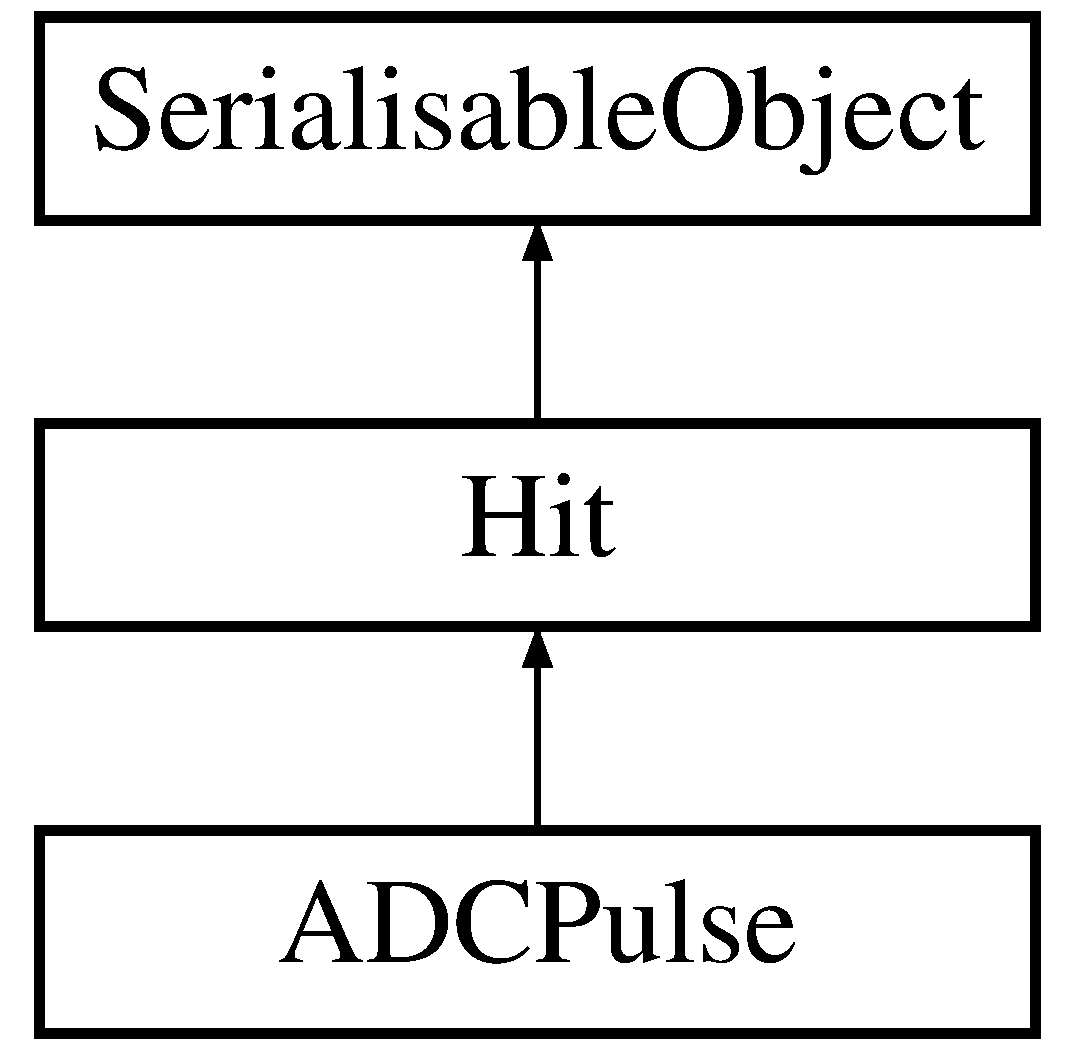
\includegraphics[height=3.000000cm]{classADCPulse}
\end{center}
\end{figure}
\subsection*{Public Member Functions}
\begin{DoxyCompactItemize}
\item 
\hypertarget{classADCPulse_a98b82ea9459a5fca7947a855fb8c7405}{{\bfseries A\-D\-C\-Pulse} (int Tube\-Id, double start\-\_\-time, double peak\-\_\-time, double baseline, double sigma\-\_\-baseline, unsigned long raw\-\_\-area, unsigned short raw\-\_\-amplitude, double calibrated\-\_\-amplitude, double charge)}\label{classADCPulse_a98b82ea9459a5fca7947a855fb8c7405}

\item 
\hypertarget{classADCPulse_aba2eb2e6400677d592ef1685ba2ae5a9}{double {\bfseries start\-\_\-time} () const }\label{classADCPulse_aba2eb2e6400677d592ef1685ba2ae5a9}

\item 
\hypertarget{classADCPulse_ac55a1faf2cf205fbdc859daece64a021}{double {\bfseries peak\-\_\-time} () const }\label{classADCPulse_ac55a1faf2cf205fbdc859daece64a021}

\item 
\hypertarget{classADCPulse_a4900e0a75c4981491f8609428888a6bc}{double {\bfseries baseline} () const }\label{classADCPulse_a4900e0a75c4981491f8609428888a6bc}

\item 
\hypertarget{classADCPulse_a824ed4ba627f7641ff70adf2fe3b026f}{double {\bfseries sigma\-\_\-baseline} () const }\label{classADCPulse_a824ed4ba627f7641ff70adf2fe3b026f}

\item 
\hypertarget{classADCPulse_a692780da124b59770356393f16299c49}{unsigned long {\bfseries raw\-\_\-area} () const }\label{classADCPulse_a692780da124b59770356393f16299c49}

\item 
\hypertarget{classADCPulse_a7a09c65e5b638c6a2df3e437219f04f8}{unsigned short {\bfseries raw\-\_\-amplitude} () const }\label{classADCPulse_a7a09c65e5b638c6a2df3e437219f04f8}

\item 
\hypertarget{classADCPulse_aad38764b5eabe9d858309bc06cf73424}{double {\bfseries charge} () const }\label{classADCPulse_aad38764b5eabe9d858309bc06cf73424}

\item 
\hypertarget{classADCPulse_adf6f2ab6b4c28e425dd7567a70099826}{double {\bfseries amplitude} () const }\label{classADCPulse_adf6f2ab6b4c28e425dd7567a70099826}

\item 
\hypertarget{classADCPulse_ae2b9e749cbd984bd1aa24dc41e4fbb73}{{\footnotesize template$<$class Archive $>$ }\\void {\bfseries serialize} (Archive \&ar, const unsigned int version)}\label{classADCPulse_ae2b9e749cbd984bd1aa24dc41e4fbb73}

\end{DoxyCompactItemize}
\subsection*{Protected Attributes}
\begin{DoxyCompactItemize}
\item 
\hypertarget{classADCPulse_af93ef20fa02d9ea44a7b84d32c8b029f}{double {\bfseries start\-\_\-time\-\_\-}}\label{classADCPulse_af93ef20fa02d9ea44a7b84d32c8b029f}

\item 
\hypertarget{classADCPulse_a4e87f35bcc0f597f6e3c3e73d0b4312b}{double {\bfseries peak\-\_\-time\-\_\-}}\label{classADCPulse_a4e87f35bcc0f597f6e3c3e73d0b4312b}

\item 
\hypertarget{classADCPulse_ab355ff3d438597f659f899e14e9ce37a}{double {\bfseries baseline\-\_\-}}\label{classADCPulse_ab355ff3d438597f659f899e14e9ce37a}

\item 
\hypertarget{classADCPulse_a97eddbc21ba72324520405c64288693e}{double {\bfseries sigma\-\_\-baseline\-\_\-}}\label{classADCPulse_a97eddbc21ba72324520405c64288693e}

\item 
\hypertarget{classADCPulse_ae665395493e477287e366b9d8772996d}{unsigned long {\bfseries raw\-\_\-area\-\_\-}}\label{classADCPulse_ae665395493e477287e366b9d8772996d}

\item 
\hypertarget{classADCPulse_ad77ade03d815b418fe138fd599f3db57}{unsigned short {\bfseries raw\-\_\-amplitude\-\_\-}}\label{classADCPulse_ad77ade03d815b418fe138fd599f3db57}

\item 
\hypertarget{classADCPulse_ae68ae047968f1257b4aa0ad9bfd08847}{double {\bfseries calibrated\-\_\-amplitude\-\_\-}}\label{classADCPulse_ae68ae047968f1257b4aa0ad9bfd08847}

\end{DoxyCompactItemize}
\subsection*{Friends}
\begin{DoxyCompactItemize}
\item 
\hypertarget{classADCPulse_ac98d07dd8f7b70e16ccb9a01abf56b9c}{class {\bfseries boost\-::serialization\-::access}}\label{classADCPulse_ac98d07dd8f7b70e16ccb9a01abf56b9c}

\end{DoxyCompactItemize}
\subsection*{Additional Inherited Members}


The documentation for this class was generated from the following files\-:\begin{DoxyCompactItemize}
\item 
Data\-Model/A\-D\-C\-Pulse.\-h\item 
Data\-Model/A\-D\-C\-Pulse.\-cpp\end{DoxyCompactItemize}

\hypertarget{classANNIEGeometry}{\section{A\-N\-N\-I\-E\-Geometry Class Reference}
\label{classANNIEGeometry}\index{A\-N\-N\-I\-E\-Geometry@{A\-N\-N\-I\-E\-Geometry}}
}
\subsection*{Public Types}
\begin{DoxyCompactItemize}
\item 
enum {\bfseries E\-Geo\-Type} \{ {\bfseries k\-Unknown} = -\/1, 
{\bfseries k\-Cylinder} = 0, 
{\bfseries k\-Mail\-Box} = 1
 \}
\item 
enum {\bfseries E\-Geo\-Region} \{ \\*
{\bfseries k\-Top} = 0, 
{\bfseries k\-Side} = 1, 
{\bfseries k\-Bottom} = 2, 
{\bfseries k\-Front} = 10, 
\\*
{\bfseries k\-Back} = 12, 
{\bfseries k\-Left} = 20, 
{\bfseries k\-Right} = 22
 \}
\item 
\hypertarget{classANNIEGeometry_ab5d29d11590e8129e6690899d0f84584}{typedef enum \\*
A\-N\-N\-I\-E\-Geometry\-::\-E\-Geo\-Type {\bfseries Geo\-Type\-\_\-t}}\label{classANNIEGeometry_ab5d29d11590e8129e6690899d0f84584}

\item 
\hypertarget{classANNIEGeometry_acf5083108f2f5a2d8ee98fe5aaa6e596}{typedef enum \\*
A\-N\-N\-I\-E\-Geometry\-::\-E\-Geo\-Region {\bfseries Geo\-Region\-\_\-t}}\label{classANNIEGeometry_acf5083108f2f5a2d8ee98fe5aaa6e596}

\end{DoxyCompactItemize}
\subsection*{Public Member Functions}
\begin{DoxyCompactItemize}
\item 
\hypertarget{classANNIEGeometry_a143bd07247da431b54d152fa7cb5c7cf}{void {\bfseries Set\-Geometry} ()}\label{classANNIEGeometry_a143bd07247da431b54d152fa7cb5c7cf}

\item 
\hypertarget{classANNIEGeometry_ab765a9957be6e19208c25fa0e6603ab7}{void {\bfseries Write\-To\-File} (const char $\ast$filename=\char`\"{}annie.\-geometry.\-root\char`\"{})}\label{classANNIEGeometry_ab765a9957be6e19208c25fa0e6603ab7}

\item 
\hypertarget{classANNIEGeometry_a4a2b51837cbc2b52159fde213624f07b}{int {\bfseries Get\-Geo\-Config} ()}\label{classANNIEGeometry_a4a2b51837cbc2b52159fde213624f07b}

\item 
\hypertarget{classANNIEGeometry_a181399c8d8d8e1e7deaf5e26fc19f6a2}{int {\bfseries Get\-Geo\-Type} ()}\label{classANNIEGeometry_a181399c8d8d8e1e7deaf5e26fc19f6a2}

\item 
\hypertarget{classANNIEGeometry_af52285d65bb359e199d5516215e9d4b2}{bool {\bfseries Is\-Cylinder} ()}\label{classANNIEGeometry_af52285d65bb359e199d5516215e9d4b2}

\item 
\hypertarget{classANNIEGeometry_af4067a89f27815d2be201734cf88ef66}{double {\bfseries Get\-Cyl\-Radius} ()}\label{classANNIEGeometry_af4067a89f27815d2be201734cf88ef66}

\item 
\hypertarget{classANNIEGeometry_aeb5d59529df45997aa9e88d439fefbba}{double {\bfseries Get\-Cyl\-Length} ()}\label{classANNIEGeometry_aeb5d59529df45997aa9e88d439fefbba}

\item 
\hypertarget{classANNIEGeometry_a3dce208ec7515a6db41b29a222ef7a4c}{double {\bfseries Get\-Cyl\-Fiducial\-Radius} ()}\label{classANNIEGeometry_a3dce208ec7515a6db41b29a222ef7a4c}

\item 
\hypertarget{classANNIEGeometry_adda169892f173736e7873a0994fa37b6}{double {\bfseries Get\-Cyl\-Fiducial\-Length} ()}\label{classANNIEGeometry_adda169892f173736e7873a0994fa37b6}

\item 
\hypertarget{classANNIEGeometry_a7675f55a9fc15b8b6e2165d641e79df9}{double {\bfseries Get\-Area} ()}\label{classANNIEGeometry_a7675f55a9fc15b8b6e2165d641e79df9}

\item 
\hypertarget{classANNIEGeometry_af0bc51ada0af21236895d9f94f2f84a7}{double {\bfseries Get\-Volume} ()}\label{classANNIEGeometry_af0bc51ada0af21236895d9f94f2f84a7}

\item 
\hypertarget{classANNIEGeometry_aa499d80e72d8d23ea302dac47c47c3ac}{double {\bfseries Get\-Fiducial\-Volume} ()}\label{classANNIEGeometry_aa499d80e72d8d23ea302dac47c47c3ac}

\item 
\hypertarget{classANNIEGeometry_a35e0bbb160a9d8aaf3a343c65d1b3e5b}{int {\bfseries Get\-Num\-P\-M\-Ts} ()}\label{classANNIEGeometry_a35e0bbb160a9d8aaf3a343c65d1b3e5b}

\item 
\hypertarget{classANNIEGeometry_ab271fef7650f1f85053e5c332923f1b2}{double {\bfseries Get\-P\-M\-T\-Radius} ()}\label{classANNIEGeometry_ab271fef7650f1f85053e5c332923f1b2}

\item 
\hypertarget{classANNIEGeometry_a6a3acf1871f9114c0a174aa776d4d568}{double {\bfseries Get\-P\-M\-T\-Coverage} ()}\label{classANNIEGeometry_a6a3acf1871f9114c0a174aa776d4d568}

\item 
\hypertarget{classANNIEGeometry_a55663b9489c6c3f8be1d8c8d50ea8ecd}{double {\bfseries Get\-P\-M\-T\-Separation} ()}\label{classANNIEGeometry_a55663b9489c6c3f8be1d8c8d50ea8ecd}

\item 
\hypertarget{classANNIEGeometry_a6186795a8e0c991456198d976987a60d}{int {\bfseries Get\-Region} (int tube)}\label{classANNIEGeometry_a6186795a8e0c991456198d976987a60d}

\item 
\hypertarget{classANNIEGeometry_a401b4205253afe89d87c9e86617fae0f}{double {\bfseries Get\-X} (int tube)}\label{classANNIEGeometry_a401b4205253afe89d87c9e86617fae0f}

\item 
\hypertarget{classANNIEGeometry_afdb90742ba6140a78d022658df6e69fc}{double {\bfseries Get\-Y} (int tube)}\label{classANNIEGeometry_afdb90742ba6140a78d022658df6e69fc}

\item 
\hypertarget{classANNIEGeometry_ae4563d14f0b5207fff374b03df026410}{double {\bfseries Get\-Z} (int tube)}\label{classANNIEGeometry_ae4563d14f0b5207fff374b03df026410}

\item 
\hypertarget{classANNIEGeometry_ab645d95b1115f411d24baa5dc868b6fb}{double {\bfseries Get\-Norm\-X} (int tube)}\label{classANNIEGeometry_ab645d95b1115f411d24baa5dc868b6fb}

\item 
\hypertarget{classANNIEGeometry_ab674db08c6e04f3f85d82f9135dbe33d}{double {\bfseries Get\-Norm\-Y} (int tube)}\label{classANNIEGeometry_ab674db08c6e04f3f85d82f9135dbe33d}

\item 
\hypertarget{classANNIEGeometry_a8dd59a80f126b58e88ab7d3008cb7001}{double {\bfseries Get\-Norm\-Z} (int tube)}\label{classANNIEGeometry_a8dd59a80f126b58e88ab7d3008cb7001}

\item 
\hypertarget{classANNIEGeometry_a8f607acd58c33b95be136fccd285588d}{bool {\bfseries Inside\-Detector} (double x, double y, double z)}\label{classANNIEGeometry_a8f607acd58c33b95be136fccd285588d}

\item 
\hypertarget{classANNIEGeometry_aad46926236afbfb92498aa1642f21180}{bool {\bfseries Inside\-Fiducial\-Volume} (double x, double y, double z)}\label{classANNIEGeometry_aad46926236afbfb92498aa1642f21180}

\item 
\hypertarget{classANNIEGeometry_a971e6acb3ee5883a3aed577831b053cf}{bool {\bfseries Inside\-Detector} (double vx, double vy, double vz, double ex, double ey, double ez)}\label{classANNIEGeometry_a971e6acb3ee5883a3aed577831b053cf}

\item 
\hypertarget{classANNIEGeometry_a9650b8008ba94cc4b53c59f67406db20}{double {\bfseries Distance\-To\-Edge} (double x, double y, double z)}\label{classANNIEGeometry_a9650b8008ba94cc4b53c59f67406db20}

\item 
\hypertarget{classANNIEGeometry_a3febbe7fd335e9618a02522d8d55a944}{void {\bfseries Project\-To\-Near\-Edge} (double x0, double y0, double z0, double px, double py, double pz, double \&x, double \&y, double \&z, int \&region)}\label{classANNIEGeometry_a3febbe7fd335e9618a02522d8d55a944}

\item 
\hypertarget{classANNIEGeometry_ac3c306909b0de82f5ddcc58de6345b16}{void {\bfseries Project\-To\-Far\-Edge} (double x0, double y0, double z0, double px, double py, double pz, double \&x, double \&y, double \&z, int \&region)}\label{classANNIEGeometry_ac3c306909b0de82f5ddcc58de6345b16}

\item 
\hypertarget{classANNIEGeometry_a88ff7bd1fcd9ed044c177ebbc875e4af}{double {\bfseries Forward\-Projection\-To\-Edge} (double x, double y, double z, double px, double py, double pz)}\label{classANNIEGeometry_a88ff7bd1fcd9ed044c177ebbc875e4af}

\item 
\hypertarget{classANNIEGeometry_adcc43a523767429765600b7c103dd5e9}{double {\bfseries Backward\-Projection\-To\-Edge} (double x, double y, double z, double px, double py, double pz)}\label{classANNIEGeometry_adcc43a523767429765600b7c103dd5e9}

\item 
\hypertarget{classANNIEGeometry_a8b4c2a1c960041a8c36c29c40bde9cb1}{void {\bfseries Project\-To\-Edge} (bool use\-Far\-Edge, double x0, double y0, double z0, double px, double py, double pz, double \&x, double \&y, double \&z, int \&region)}\label{classANNIEGeometry_a8b4c2a1c960041a8c36c29c40bde9cb1}

\item 
\hypertarget{classANNIEGeometry_a8b839b45c5eace4880b79d451b6e6f29}{void {\bfseries X\-Y\-Zto\-U\-V} (int region, double x, double y, double z, double \&u, double \&v)}\label{classANNIEGeometry_a8b839b45c5eace4880b79d451b6e6f29}

\end{DoxyCompactItemize}
\subsection*{Static Public Member Functions}
\begin{DoxyCompactItemize}
\item 
\hypertarget{classANNIEGeometry_ac5019e6c5628d0381760a43169b1f69c}{static \hyperlink{classANNIEGeometry}{A\-N\-N\-I\-E\-Geometry} $\ast$ {\bfseries Instance} ()}\label{classANNIEGeometry_ac5019e6c5628d0381760a43169b1f69c}

\item 
\hypertarget{classANNIEGeometry_ad5cc6f1a59adcc81ed32baf70fffe80a}{static void {\bfseries Build\-Geometry} ()}\label{classANNIEGeometry_ad5cc6f1a59adcc81ed32baf70fffe80a}

\item 
\hypertarget{classANNIEGeometry_a263767eee59a5cf354f3f78ff11efe15}{static void {\bfseries Print\-Geometry} ()}\label{classANNIEGeometry_a263767eee59a5cf354f3f78ff11efe15}

\item 
\hypertarget{classANNIEGeometry_ae6ac4bbd93009837fb6dd876eec7a558}{static void {\bfseries Write\-Geometry} (const char $\ast$filename=\char`\"{}annie.\-geometry.\-root\char`\"{})}\label{classANNIEGeometry_ae6ac4bbd93009837fb6dd876eec7a558}

\item 
\hypertarget{classANNIEGeometry_a1bb496b1b3f0f3ef86a76dc59571beb7}{static bool {\bfseries Touch\-Geometry} ()}\label{classANNIEGeometry_a1bb496b1b3f0f3ef86a76dc59571beb7}

\item 
\hypertarget{classANNIEGeometry_a8d2c6faa5bdc504fb70967551ad59068}{static void {\bfseries Reset} ()}\label{classANNIEGeometry_a8d2c6faa5bdc504fb70967551ad59068}

\item 
\hypertarget{classANNIEGeometry_a6de654c497e0f352fc293cfc87246a0f}{static void {\bfseries Find\-Circle} (double x0, double y0, double z0, double x1, double y1, double z1, double x2, double y2, double z2, double \&rx, double \&ry, double \&rz, double \&nx, double \&ny, double \&nz, double \&r)}\label{classANNIEGeometry_a6de654c497e0f352fc293cfc87246a0f}

\item 
\hypertarget{classANNIEGeometry_ab8f9b0fa3e34b1524146e536cb0d61b8}{static void {\bfseries Find\-Circle} (double xp, double yp, double zp, double x0, double y0, double z0, double angle\-\_\-degrees, double omega\-\_\-degrees, double \&rx, double \&ry, double \&rz, double \&nx, double \&ny, double \&nz, double \&r)}\label{classANNIEGeometry_ab8f9b0fa3e34b1524146e536cb0d61b8}

\item 
\hypertarget{classANNIEGeometry_a9b64b97c795a3ff52ff8473b844949ab}{static void {\bfseries Find\-Circle\-Old} (double xp, double yp, double zp, double x0, double y0, double z0, double angle\-\_\-degrees, double omega\-\_\-degrees, double \&rx, double \&ry, double \&rz, double \&nx, double \&ny, double \&nz, double \&r)}\label{classANNIEGeometry_a9b64b97c795a3ff52ff8473b844949ab}

\item 
\hypertarget{classANNIEGeometry_a84d4314f64f749a0a7c9a771805226dc}{static void {\bfseries Find\-Vertex} (double x0, double y0, double z0, double t0, double x1, double y1, double z1, double t1, double x2, double y2, double z2, double t2, double x3, double y3, double z3, double t3, double \&vxm, double \&vym, double \&vzm, double \&vtm, double \&vxp, double \&vyp, double \&vzp, double \&vtp)}\label{classANNIEGeometry_a84d4314f64f749a0a7c9a771805226dc}

\item 
\hypertarget{classANNIEGeometry_a3ad5ab10afc05105f6be10e87fb69227}{static void {\bfseries Distance\-To\-Intersect\-Line} (double x0, double y0, double z0, double vx, double vy, double vz, double ex, double ey, double ez, double \&x, double \&y, double \&z, double \&L)}\label{classANNIEGeometry_a3ad5ab10afc05105f6be10e87fb69227}

\item 
\hypertarget{classANNIEGeometry_a7564706390f93705700a15d4cf4f43a6}{static double {\bfseries Distance\-To\-Intersect\-Line} (double x0, double y0, double z0, double sx, double sy, double sz, double ex, double ey, double ez, double \&x, double \&y, double \&z)}\label{classANNIEGeometry_a7564706390f93705700a15d4cf4f43a6}

\item 
\hypertarget{classANNIEGeometry_ac39690635de68c00b8c806fcca9ff597}{static double {\bfseries Distance\-To\-Intersect\-Line} (double $\ast$pos, double $\ast$start, double $\ast$end, double $\ast$intersection)}\label{classANNIEGeometry_ac39690635de68c00b8c806fcca9ff597}

\end{DoxyCompactItemize}


The documentation for this class was generated from the following files\-:\begin{DoxyCompactItemize}
\item 
Data\-Model/A\-N\-N\-I\-E\-Geometry.\-h\item 
Data\-Model/A\-N\-N\-I\-E\-Geometry.\-cpp\end{DoxyCompactItemize}

\hypertarget{classANNIERecoObjectTable}{
\section{ANNIERecoObjectTable Class Reference}
\label{classANNIERecoObjectTable}\index{ANNIERecoObjectTable@{ANNIERecoObjectTable}}
}
\subsection*{Public Member Functions}
\begin{DoxyCompactItemize}
\item 
\hypertarget{classANNIERecoObjectTable_ae2e86010f9f57ce6044d084ec40f475b}{
void {\bfseries NewDigit} ()}
\label{classANNIERecoObjectTable_ae2e86010f9f57ce6044d084ec40f475b}

\item 
\hypertarget{classANNIERecoObjectTable_a75f289f8c9eef9098813dbdcc8ddd518}{
void {\bfseries DeleteDigit} ()}
\label{classANNIERecoObjectTable_a75f289f8c9eef9098813dbdcc8ddd518}

\item 
\hypertarget{classANNIERecoObjectTable_a6a91ff418f86119ef35de20c5c9a9e8a}{
Int\_\-t {\bfseries NumberOfDigits} ()}
\label{classANNIERecoObjectTable_a6a91ff418f86119ef35de20c5c9a9e8a}

\item 
\hypertarget{classANNIERecoObjectTable_a4bbb7e3eb5ca8a46486a1087ef2b4ff1}{
void {\bfseries NewCluster} ()}
\label{classANNIERecoObjectTable_a4bbb7e3eb5ca8a46486a1087ef2b4ff1}

\item 
\hypertarget{classANNIERecoObjectTable_a77fe22b611dbc374779bf258eae901a2}{
void {\bfseries DeleteCluster} ()}
\label{classANNIERecoObjectTable_a77fe22b611dbc374779bf258eae901a2}

\item 
\hypertarget{classANNIERecoObjectTable_a87c83bd73d95b7bc2fca9855e8604496}{
Int\_\-t {\bfseries NumberOfClusters} ()}
\label{classANNIERecoObjectTable_a87c83bd73d95b7bc2fca9855e8604496}

\item 
\hypertarget{classANNIERecoObjectTable_ae5d19c03be8a404512ddad75e76be951}{
void {\bfseries NewClusterDigit} ()}
\label{classANNIERecoObjectTable_ae5d19c03be8a404512ddad75e76be951}

\item 
\hypertarget{classANNIERecoObjectTable_ae9e239382fa31db834474b4307959f1b}{
void {\bfseries DeleteClusterDigit} ()}
\label{classANNIERecoObjectTable_ae9e239382fa31db834474b4307959f1b}

\item 
\hypertarget{classANNIERecoObjectTable_a6b1f8a751bd988ea99bb1dcd04e355f1}{
Int\_\-t {\bfseries NumberOfClusterDigits} ()}
\label{classANNIERecoObjectTable_a6b1f8a751bd988ea99bb1dcd04e355f1}

\item 
\hypertarget{classANNIERecoObjectTable_a27ba37a8270a06fd8a60334e94c5ccc7}{
void {\bfseries NewVertex} ()}
\label{classANNIERecoObjectTable_a27ba37a8270a06fd8a60334e94c5ccc7}

\item 
\hypertarget{classANNIERecoObjectTable_a51a949a392b138359f6c3e3a91a17815}{
void {\bfseries DeleteVertex} ()}
\label{classANNIERecoObjectTable_a51a949a392b138359f6c3e3a91a17815}

\item 
\hypertarget{classANNIERecoObjectTable_ad96ca7367ce386c39b33fe7028481fed}{
Int\_\-t {\bfseries NumberOfVertices} ()}
\label{classANNIERecoObjectTable_ad96ca7367ce386c39b33fe7028481fed}

\item 
\hypertarget{classANNIERecoObjectTable_a44fea21839a6a27ea162659799d64b9e}{
void {\bfseries NewRing} ()}
\label{classANNIERecoObjectTable_a44fea21839a6a27ea162659799d64b9e}

\item 
\hypertarget{classANNIERecoObjectTable_a91992ce4b239b292ea3e8300b6f3d051}{
void {\bfseries DeleteRing} ()}
\label{classANNIERecoObjectTable_a91992ce4b239b292ea3e8300b6f3d051}

\item 
\hypertarget{classANNIERecoObjectTable_a6f4586ab138e3de6e2d0445f9a42158e}{
Int\_\-t {\bfseries NumberOfRings} ()}
\label{classANNIERecoObjectTable_a6f4586ab138e3de6e2d0445f9a42158e}

\item 
\hypertarget{classANNIERecoObjectTable_a40d63437190711714ef1a0e2323e552b}{
void {\bfseries NewEvent} ()}
\label{classANNIERecoObjectTable_a40d63437190711714ef1a0e2323e552b}

\item 
\hypertarget{classANNIERecoObjectTable_ad9e81e1ef88bb6c19359465cf1897489}{
void {\bfseries DeleteEvent} ()}
\label{classANNIERecoObjectTable_ad9e81e1ef88bb6c19359465cf1897489}

\item 
\hypertarget{classANNIERecoObjectTable_a2802d7f20a163c710703ede7b66ba02f}{
Int\_\-t {\bfseries NumberOfEvents} ()}
\label{classANNIERecoObjectTable_a2802d7f20a163c710703ede7b66ba02f}

\item 
\hypertarget{classANNIERecoObjectTable_ae0f39f0d4b6392330fe449f22b3a5481}{
void {\bfseries Reset} ()}
\label{classANNIERecoObjectTable_ae0f39f0d4b6392330fe449f22b3a5481}

\item 
\hypertarget{classANNIERecoObjectTable_a620e131ba8cf125b7f08f25d19ee14c1}{
void {\bfseries Print} ()}
\label{classANNIERecoObjectTable_a620e131ba8cf125b7f08f25d19ee14c1}

\end{DoxyCompactItemize}
\subsection*{Static Public Member Functions}
\begin{DoxyCompactItemize}
\item 
\hypertarget{classANNIERecoObjectTable_a2d52c0a9b2ed24f59c97ae6cfff3b1f6}{
static \hyperlink{classANNIERecoObjectTable}{ANNIERecoObjectTable} $\ast$ {\bfseries Instance} ()}
\label{classANNIERecoObjectTable_a2d52c0a9b2ed24f59c97ae6cfff3b1f6}

\end{DoxyCompactItemize}


The documentation for this class was generated from the following files:\begin{DoxyCompactItemize}
\item 
DataModel/ANNIERecoObjectTable.h\item 
DataModel/ANNIERecoObjectTable.cpp\end{DoxyCompactItemize}

\hypertarget{classBeamChecker}{\section{Beam\-Checker Class Reference}
\label{classBeamChecker}\index{Beam\-Checker@{Beam\-Checker}}
}
Inheritance diagram for Beam\-Checker\-:\begin{figure}[H]
\begin{center}
\leavevmode
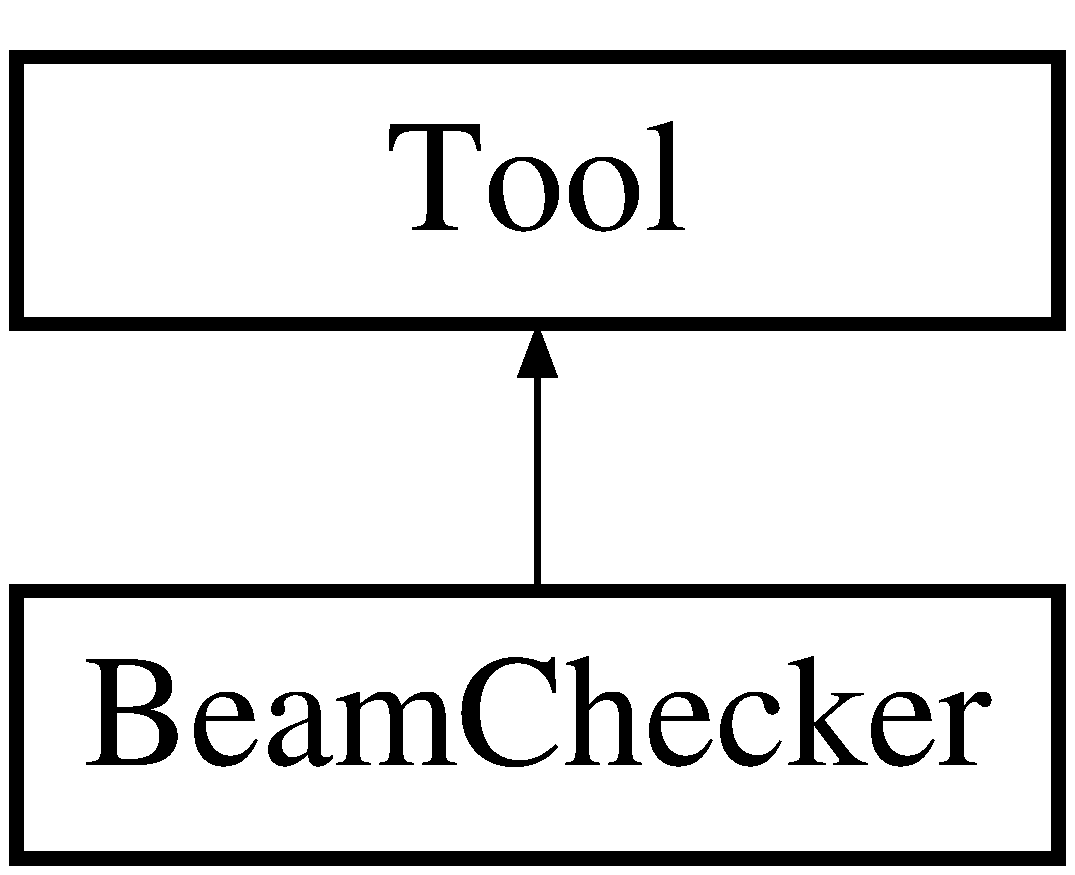
\includegraphics[height=2.000000cm]{classBeamChecker}
\end{center}
\end{figure}
\subsection*{Public Member Functions}
\begin{DoxyCompactItemize}
\item 
\hypertarget{classBeamChecker_a8025fea06b24c363f17764b3cc049ebd}{bool {\bfseries Initialise} (std\-::string configfile, \hyperlink{classDataModel}{Data\-Model} \&data)}\label{classBeamChecker_a8025fea06b24c363f17764b3cc049ebd}

\item 
\hypertarget{classBeamChecker_a9fd96575f736c2a0a90e9b18fca3bdf7}{bool {\bfseries Execute} ()}\label{classBeamChecker_a9fd96575f736c2a0a90e9b18fca3bdf7}

\item 
\hypertarget{classBeamChecker_a1f9078a610f387f97dc6d17a6b98f493}{bool {\bfseries Finalise} ()}\label{classBeamChecker_a1f9078a610f387f97dc6d17a6b98f493}

\end{DoxyCompactItemize}
\subsection*{Protected Member Functions}
\begin{DoxyCompactItemize}
\item 
\hypertarget{classBeamChecker_a85643380e26692a3fad55cc4e7d4ea1b}{bool \hyperlink{classBeamChecker_a85643380e26692a3fad55cc4e7d4ea1b}{initialise\-\_\-beam\-\_\-db} ()}\label{classBeamChecker_a85643380e26692a3fad55cc4e7d4ea1b}

\begin{DoxyCompactList}\small\item\em Helper function that opens the beam database data file and loads the Beam\-D\-B Boost\-Store. \end{DoxyCompactList}\item 
\hypertarget{classBeamChecker_a40e731049d58aa141a15f3431b00a764}{\hyperlink{classBeamStatus}{Beam\-Status} {\bfseries get\-\_\-beam\-\_\-status} (uint64\-\_\-t ns\-\_\-since\-\_\-epoch, Minibuffer\-Label mb\-\_\-label)}\label{classBeamChecker_a40e731049d58aa141a15f3431b00a764}

\end{DoxyCompactItemize}
\subsection*{Protected Attributes}
\begin{DoxyCompactItemize}
\item 
\hypertarget{classBeamChecker_a2b910738f1f07819ce8cf564bff685d0}{Boost\-Store \hyperlink{classBeamChecker_a2b910738f1f07819ce8cf564bff685d0}{beam\-\_\-db\-\_\-store\-\_\-}}\label{classBeamChecker_a2b910738f1f07819ce8cf564bff685d0}

\begin{DoxyCompactList}\small\item\em Transient Boost\-Store used to read previously-\/saved information from the beam database. \end{DoxyCompactList}\item 
std\-::map$<$ int, std\-::pair\\*
$<$ uint64\-\_\-t, uint64\-\_\-t $>$ $>$ \hyperlink{classBeamChecker_aab9b16fbdd8cdea6aa1a77fc2f0ea842}{beam\-\_\-db\-\_\-index\-\_\-}
\begin{DoxyCompactList}\small\item\em Map that enables quick searches of the beam database Boost\-Store. \end{DoxyCompactList}\item 
int \hyperlink{classBeamChecker_aceafb01556c2541a737d4feaab2f757e}{verbosity\-\_\-}
\begin{DoxyCompactList}\small\item\em The verbosity to use when printing logging messages. \end{DoxyCompactList}\item 
\hypertarget{classBeamChecker_acd0db6480aaf42ee431b182a68496c32}{uint64\-\_\-t \hyperlink{classBeamChecker_acd0db6480aaf42ee431b182a68496c32}{start\-\_\-ms\-\_\-since\-\_\-epoch\-\_\-}}\label{classBeamChecker_acd0db6480aaf42ee431b182a68496c32}

\begin{DoxyCompactList}\small\item\em The timestamp (ms since the Unix epoch) of the earliest P\-O\-T information available in the current beam database file. \end{DoxyCompactList}\item 
\hypertarget{classBeamChecker_abb2801b7c15da8c7ae56f96786d6cb54}{uint64\-\_\-t \hyperlink{classBeamChecker_abb2801b7c15da8c7ae56f96786d6cb54}{end\-\_\-ms\-\_\-since\-\_\-epoch\-\_\-}}\label{classBeamChecker_abb2801b7c15da8c7ae56f96786d6cb54}

\begin{DoxyCompactList}\small\item\em The timestamp (ms since the Unix epoch) of the latest P\-O\-T information available in the current beam database file. \end{DoxyCompactList}\end{DoxyCompactItemize}


\subsection{Member Data Documentation}
\hypertarget{classBeamChecker_aab9b16fbdd8cdea6aa1a77fc2f0ea842}{\index{Beam\-Checker@{Beam\-Checker}!beam\-\_\-db\-\_\-index\-\_\-@{beam\-\_\-db\-\_\-index\-\_\-}}
\index{beam\-\_\-db\-\_\-index\-\_\-@{beam\-\_\-db\-\_\-index\-\_\-}!BeamChecker@{Beam\-Checker}}
\subsubsection[{beam\-\_\-db\-\_\-index\-\_\-}]{\setlength{\rightskip}{0pt plus 5cm}std\-::map$<$int, std\-::pair$<$uint64\-\_\-t, uint64\-\_\-t$>$ $>$ Beam\-Checker\-::beam\-\_\-db\-\_\-index\-\_\-\hspace{0.3cm}{\ttfamily [protected]}}}\label{classBeamChecker_aab9b16fbdd8cdea6aa1a77fc2f0ea842}


Map that enables quick searches of the beam database Boost\-Store. 

Keys are entry numbers in the Beam\-Data T\-Tree, values are (start time, end time) pairs giving the range of times (in ms since the Unix epoch) recorded for the E\-:T\-O\-R875 device (used to determine P\-O\-T values) in each entry \hypertarget{classBeamChecker_aceafb01556c2541a737d4feaab2f757e}{\index{Beam\-Checker@{Beam\-Checker}!verbosity\-\_\-@{verbosity\-\_\-}}
\index{verbosity\-\_\-@{verbosity\-\_\-}!BeamChecker@{Beam\-Checker}}
\subsubsection[{verbosity\-\_\-}]{\setlength{\rightskip}{0pt plus 5cm}int Beam\-Checker\-::verbosity\-\_\-\hspace{0.3cm}{\ttfamily [protected]}}}\label{classBeamChecker_aceafb01556c2541a737d4feaab2f757e}


The verbosity to use when printing logging messages. 

A larger value corresponds to more verbose output 

The documentation for this class was generated from the following files\-:\begin{DoxyCompactItemize}
\item 
User\-Tools/\-Beam\-Checker/Beam\-Checker.\-h\item 
User\-Tools/\-Beam\-Checker/Beam\-Checker.\-cpp\end{DoxyCompactItemize}

\hypertarget{structBeamDataPoint}{
\section{BeamDataPoint Struct Reference}
\label{structBeamDataPoint}\index{BeamDataPoint@{BeamDataPoint}}
}


Container to hold values from Intensity Frontier beam database queries, together with their associated units.  


{\ttfamily \#include $<$BeamDataPoint.h$>$}Inheritance diagram for BeamDataPoint::\begin{figure}[H]
\begin{center}
\leavevmode
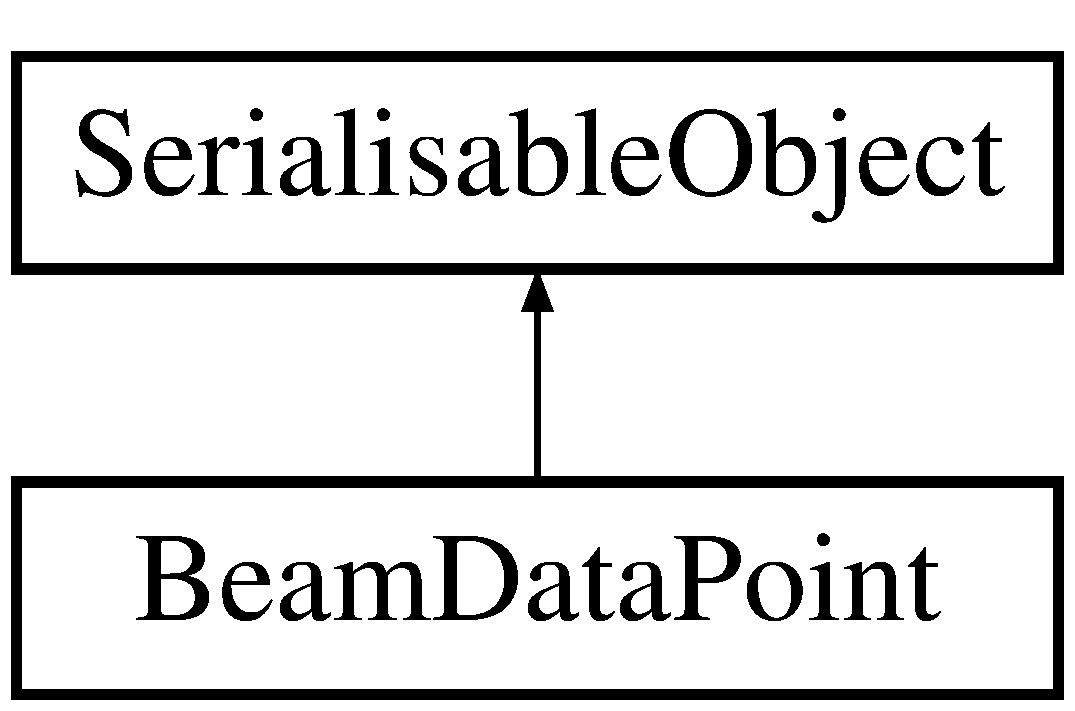
\includegraphics[height=2cm]{structBeamDataPoint}
\end{center}
\end{figure}
\subsection*{Public Member Functions}
\begin{DoxyCompactItemize}
\item 
\hypertarget{structBeamDataPoint_ad98646938f8e5337563523d7d0a198b4}{
{\bfseries BeamDataPoint} (double Value, const std::string \&Unit)}
\label{structBeamDataPoint_ad98646938f8e5337563523d7d0a198b4}

\item 
\hypertarget{structBeamDataPoint_a4da3cbcb61af8e7acc0c5b13c0a2ec32}{
{\footnotesize template$<$class Archive $>$ }\\void {\bfseries serialize} (Archive \&ar, const unsigned int version)}
\label{structBeamDataPoint_a4da3cbcb61af8e7acc0c5b13c0a2ec32}

\item 
\hypertarget{structBeamDataPoint_aaa7b4c28dfad7d79f92c6d60001d36ac}{
virtual bool {\bfseries Print} () override}
\label{structBeamDataPoint_aaa7b4c28dfad7d79f92c6d60001d36ac}

\end{DoxyCompactItemize}
\subsection*{Public Attributes}
\begin{DoxyCompactItemize}
\item 
\hypertarget{structBeamDataPoint_ab877fc81dd293f30ec6475f9649cddd0}{
double {\bfseries value}}
\label{structBeamDataPoint_ab877fc81dd293f30ec6475f9649cddd0}

\item 
\hypertarget{structBeamDataPoint_a0a0e275d6a6bc2631c4103eb7e2b44e4}{
std::string {\bfseries unit}}
\label{structBeamDataPoint_a0a0e275d6a6bc2631c4103eb7e2b44e4}

\end{DoxyCompactItemize}
\subsection*{Friends}
\begin{DoxyCompactItemize}
\item 
\hypertarget{structBeamDataPoint_ac98d07dd8f7b70e16ccb9a01abf56b9c}{
class {\bfseries boost::serialization::access}}
\label{structBeamDataPoint_ac98d07dd8f7b70e16ccb9a01abf56b9c}

\end{DoxyCompactItemize}


\subsection{Detailed Description}
Container to hold values from Intensity Frontier beam database queries, together with their associated units. 

The documentation for this struct was generated from the following file:\begin{DoxyCompactItemize}
\item 
DataModel/BeamDataPoint.h\end{DoxyCompactItemize}

\hypertarget{classBeamFetcher}{
\section{BeamFetcher Class Reference}
\label{classBeamFetcher}\index{BeamFetcher@{BeamFetcher}}
}
\subsection*{Public Member Functions}
\begin{DoxyCompactItemize}
\item 
\hypertarget{classBeamFetcher_a575275aab7b03eb11cafd132fcce3015}{
bool {\bfseries Initialise} (std::string configfile, \hyperlink{classDataModel}{DataModel} \&data)}
\label{classBeamFetcher_a575275aab7b03eb11cafd132fcce3015}

\item 
\hypertarget{classBeamFetcher_afb3681ee1fbe9ea81c6268af05b90a5f}{
bool {\bfseries Execute} ()}
\label{classBeamFetcher_afb3681ee1fbe9ea81c6268af05b90a5f}

\item 
\hypertarget{classBeamFetcher_ae69fe473f0e6d24685eb9e234d97d172}{
bool {\bfseries Finalise} ()}
\label{classBeamFetcher_ae69fe473f0e6d24685eb9e234d97d172}

\end{DoxyCompactItemize}
\subsection*{Protected Member Functions}
\begin{DoxyCompactItemize}
\item 
\hypertarget{classBeamFetcher_a60c8d28364654bc042de262cacc94dcb}{
bool \hyperlink{classBeamFetcher_a60c8d28364654bc042de262cacc94dcb}{fetch\_\-beam\_\-data} (uint64\_\-t start\_\-ms\_\-since\_\-epoch, uint64\_\-t end\_\-ms\_\-since\_\-epoch, uint64\_\-t chunk\_\-step\_\-ms)}
\label{classBeamFetcher_a60c8d28364654bc042de262cacc94dcb}

\begin{DoxyCompactList}\small\item\em Helper function that downloads and processes the beam information. \item\end{DoxyCompactList}\end{DoxyCompactItemize}
\subsection*{Protected Attributes}
\begin{DoxyCompactItemize}
\item 
int \hyperlink{classBeamFetcher_ab78e5092f1cd5b0544fe6b587282c968}{verbosity\_\-}
\begin{DoxyCompactList}\small\item\em The verbosity to use when printing logging messages. \item\end{DoxyCompactList}\item 
\hypertarget{classBeamFetcher_ac9e8e1c53a2f06c00be83258be22400d}{
BoostStore \hyperlink{classBeamFetcher_ac9e8e1c53a2f06c00be83258be22400d}{beam\_\-db\_\-store\_\-}}
\label{classBeamFetcher_ac9e8e1c53a2f06c00be83258be22400d}

\begin{DoxyCompactList}\small\item\em Transient BoostStore used to save downloaded information from the Intensity Frontier beam database to disk. \item\end{DoxyCompactList}\item 
\hypertarget{classBeamFetcher_a6e37759beec5bc578d7d4de539329bce}{
std::string \hyperlink{classBeamFetcher_a6e37759beec5bc578d7d4de539329bce}{db\_\-filename\_\-}}
\label{classBeamFetcher_a6e37759beec5bc578d7d4de539329bce}

\begin{DoxyCompactList}\small\item\em Name of the output file in which the beam database information will be saved. \item\end{DoxyCompactList}\end{DoxyCompactItemize}


\subsection{Member Data Documentation}
\hypertarget{classBeamFetcher_ab78e5092f1cd5b0544fe6b587282c968}{
\index{BeamFetcher@{BeamFetcher}!verbosity\_\-@{verbosity\_\-}}
\index{verbosity\_\-@{verbosity\_\-}!BeamFetcher@{BeamFetcher}}
\subsubsection[{verbosity\_\-}]{\setlength{\rightskip}{0pt plus 5cm}int {\bf BeamFetcher::verbosity\_\-}\hspace{0.3cm}{\ttfamily  \mbox{[}protected\mbox{]}}}}
\label{classBeamFetcher_ab78e5092f1cd5b0544fe6b587282c968}


The verbosity to use when printing logging messages. A larger value corresponds to more verbose output 

The documentation for this class was generated from the following files:\begin{DoxyCompactItemize}
\item 
UserTools/BeamFetcher/BeamFetcher.h\item 
UserTools/BeamFetcher/BeamFetcher.cpp\end{DoxyCompactItemize}

\hypertarget{classBeamStatus}{\section{Beam\-Status Class Reference}
\label{classBeamStatus}\index{Beam\-Status@{Beam\-Status}}
}
Inheritance diagram for Beam\-Status\-:\begin{figure}[H]
\begin{center}
\leavevmode
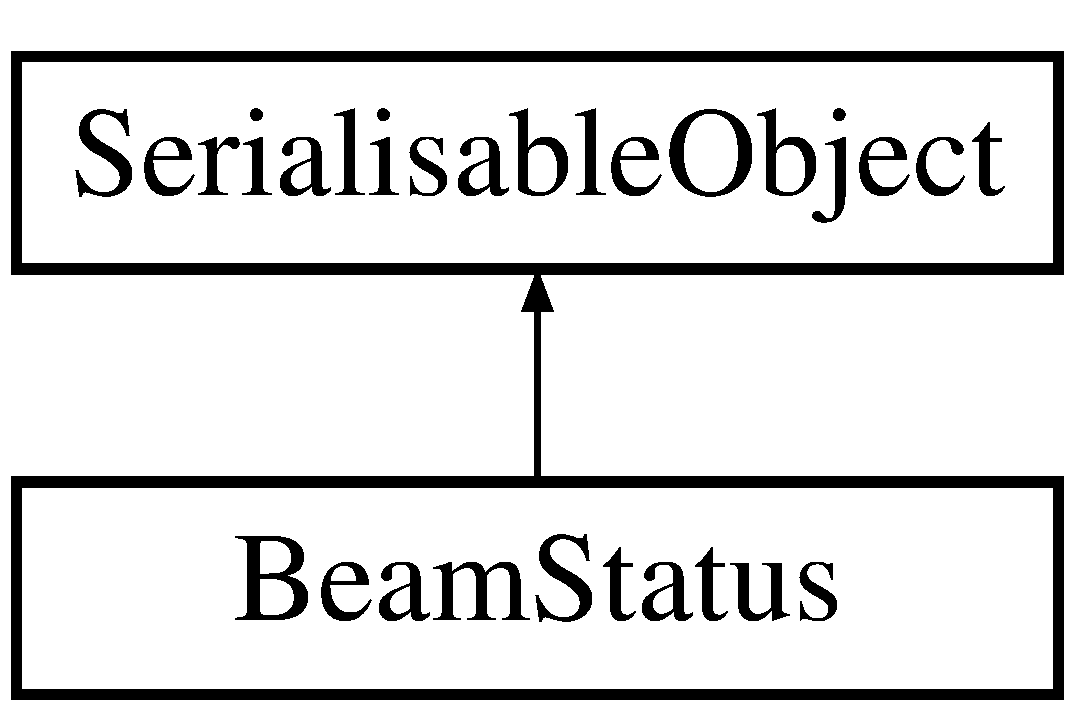
\includegraphics[height=2.000000cm]{classBeamStatus}
\end{center}
\end{figure}
\subsection*{Public Member Functions}
\begin{DoxyCompactItemize}
\item 
\hypertarget{classBeamStatus_a8763cbecad2a03bdc4d4799fd2d68569}{{\bfseries Beam\-Status} (\hyperlink{classTimeClass}{Time\-Class} time, double P\-O\-T, Beam\-Condition condition=Beam\-Condition\-::\-Missing)}\label{classBeamStatus_a8763cbecad2a03bdc4d4799fd2d68569}

\item 
\hypertarget{classBeamStatus_ad9786a1628d6180d3abbc74daef3d677}{void {\bfseries clear} ()}\label{classBeamStatus_ad9786a1628d6180d3abbc74daef3d677}

\item 
\hypertarget{classBeamStatus_a041fe2a720d2c24391fdaa578754e315}{\hyperlink{classTimeClass}{Time\-Class} {\bfseries time} () const }\label{classBeamStatus_a041fe2a720d2c24391fdaa578754e315}

\item 
\hypertarget{classBeamStatus_a234b45ea673b396d29b4a40061c633c9}{double {\bfseries pot} () const }\label{classBeamStatus_a234b45ea673b396d29b4a40061c633c9}

\item 
\hypertarget{classBeamStatus_a1e0b28ff6f6e0fdc60242e395d836dca}{Beam\-Condition {\bfseries condition} () const }\label{classBeamStatus_a1e0b28ff6f6e0fdc60242e395d836dca}

\item 
\hypertarget{classBeamStatus_a0d1a612eece988337b69b39b73d8170e}{const std\-::map$<$ std\-::string, \\*
std\-::pair$<$ uint64\-\_\-t, \\*
\hyperlink{structBeamDataPoint}{Beam\-Data\-Point} $>$ $>$ \& {\bfseries data} () const }\label{classBeamStatus_a0d1a612eece988337b69b39b73d8170e}

\item 
\hypertarget{classBeamStatus_a4b0a3f4fcce7aa7e3fa1e62c6f833d57}{const std\-::map$<$ std\-::string, \\*
bool $>$ \& {\bfseries cuts} () const }\label{classBeamStatus_a4b0a3f4fcce7aa7e3fa1e62c6f833d57}

\item 
\hypertarget{classBeamStatus_a106c1657c2cc64e76fac1179ba411485}{bool {\bfseries is\-\_\-beam} () const }\label{classBeamStatus_a106c1657c2cc64e76fac1179ba411485}

\item 
\hypertarget{classBeamStatus_a81a21d4debb9d1497024398bd8834ba3}{bool {\bfseries is\-\_\-missing} () const }\label{classBeamStatus_a81a21d4debb9d1497024398bd8834ba3}

\item 
\hypertarget{classBeamStatus_af51602157cd9beb020fd01cc72dd95cd}{bool {\bfseries is\-\_\-bad} () const }\label{classBeamStatus_af51602157cd9beb020fd01cc72dd95cd}

\item 
\hypertarget{classBeamStatus_aba458d6774b27d401b393de038668849}{bool {\bfseries ok} () const }\label{classBeamStatus_aba458d6774b27d401b393de038668849}

\item 
\hypertarget{classBeamStatus_ab6b42b298203d0df45cfb46686d491c2}{bool {\bfseries passed\-\_\-cut} (const std\-::string \&cut\-\_\-name) const }\label{classBeamStatus_ab6b42b298203d0df45cfb46686d491c2}

\item 
\hypertarget{classBeamStatus_a34ae2eee9aeb8bfe54d176455e6caaa4}{bool {\bfseries passed\-\_\-all\-\_\-cuts} () const }\label{classBeamStatus_a34ae2eee9aeb8bfe54d176455e6caaa4}

\item 
\hypertarget{classBeamStatus_aa92b44fce12d6ed0a9a14adcdb95487a}{void {\bfseries set\-\_\-time} (\hyperlink{classTimeClass}{Time\-Class} time)}\label{classBeamStatus_aa92b44fce12d6ed0a9a14adcdb95487a}

\item 
\hypertarget{classBeamStatus_a298a8def6b655bf601a73cd0f27ec5b1}{void {\bfseries set\-\_\-pot} (double P\-O\-T)}\label{classBeamStatus_a298a8def6b655bf601a73cd0f27ec5b1}

\item 
\hypertarget{classBeamStatus_aff21cffb9bcc0562b0940839f80b30f4}{void {\bfseries set\-\_\-condition} (Beam\-Condition bc)}\label{classBeamStatus_aff21cffb9bcc0562b0940839f80b30f4}

\item 
\hypertarget{classBeamStatus_a088f4dc4e0db476f939314e6c596ee1c}{void {\bfseries add\-\_\-measurement} (const std\-::string \&device\-\_\-name, uint64\-\_\-t ms\-\_\-since\-\_\-epoch, const \hyperlink{structBeamDataPoint}{Beam\-Data\-Point} \&bdp)}\label{classBeamStatus_a088f4dc4e0db476f939314e6c596ee1c}

\item 
\hypertarget{classBeamStatus_a5ea13f02f3addd9c9cfc406d461db5db}{void {\bfseries add\-\_\-measurement} (const std\-::string \&device\-\_\-name, uint64\-\_\-t ms\-\_\-since\-\_\-epoch, double value, const std\-::string \&unit)}\label{classBeamStatus_a5ea13f02f3addd9c9cfc406d461db5db}

\item 
\hypertarget{classBeamStatus_add23dfa0ed263857cd9f734815051b9a}{void {\bfseries add\-\_\-cut} (const std\-::string \&cut\-\_\-name, bool passed)}\label{classBeamStatus_add23dfa0ed263857cd9f734815051b9a}

\item 
\hypertarget{classBeamStatus_a9c074d793c6a5e55d12265895c736d9e}{bool {\bfseries Print} ()}\label{classBeamStatus_a9c074d793c6a5e55d12265895c736d9e}

\end{DoxyCompactItemize}
\subsection*{Protected Member Functions}
\begin{DoxyCompactItemize}
\item 
\hypertarget{classBeamStatus_ad7450d8c7fd19ab5020381dca6f801e8}{{\footnotesize template$<$class Archive $>$ }\\void {\bfseries serialize} (Archive \&ar, const unsigned int version)}\label{classBeamStatus_ad7450d8c7fd19ab5020381dca6f801e8}

\end{DoxyCompactItemize}
\subsection*{Protected Attributes}
\begin{DoxyCompactItemize}
\item 
\hyperlink{classTimeClass}{Time\-Class} \hyperlink{classBeamStatus_a499b220ec0c80ce883d19f8f9520934d}{time\-\_\-}
\begin{DoxyCompactList}\small\item\em The timestamp from the beam database used to assign a P\-O\-T value to the current minibuffer (ns since the Unix epoch) \end{DoxyCompactList}\item 
\hypertarget{classBeamStatus_ab4d86e7e924a02a73324105931e5bdc5}{double \hyperlink{classBeamStatus_ab4d86e7e924a02a73324105931e5bdc5}{pot\-\_\-}}\label{classBeamStatus_ab4d86e7e924a02a73324105931e5bdc5}

\begin{DoxyCompactList}\small\item\em Protons on target. \end{DoxyCompactList}\item 
Beam\-Condition \hyperlink{classBeamStatus_a8e81a7fca77f64c2ce0e41bd0e14c3ea}{condition\-\_\-}
\begin{DoxyCompactList}\small\item\em Enum class describing whether the data can be trusted. \end{DoxyCompactList}\item 
\hypertarget{classBeamStatus_a784e81454e78fc90f3c8206d68cae144}{std\-::map$<$ std\-::string, \\*
std\-::pair$<$ uint64\-\_\-t, \\*
\hyperlink{structBeamDataPoint}{Beam\-Data\-Point} $>$ $>$ {\bfseries data\-\_\-}}\label{classBeamStatus_a784e81454e78fc90f3c8206d68cae144}

\item 
\hypertarget{classBeamStatus_aff0365d2d921712d77e96fabfbcebdc3}{std\-::map$<$ std\-::string, bool $>$ {\bfseries cuts\-\_\-}}\label{classBeamStatus_aff0365d2d921712d77e96fabfbcebdc3}

\end{DoxyCompactItemize}
\subsection*{Friends}
\begin{DoxyCompactItemize}
\item 
\hypertarget{classBeamStatus_ac98d07dd8f7b70e16ccb9a01abf56b9c}{class {\bfseries boost\-::serialization\-::access}}\label{classBeamStatus_ac98d07dd8f7b70e16ccb9a01abf56b9c}

\end{DoxyCompactItemize}


\subsection{Member Data Documentation}
\hypertarget{classBeamStatus_a8e81a7fca77f64c2ce0e41bd0e14c3ea}{\index{Beam\-Status@{Beam\-Status}!condition\-\_\-@{condition\-\_\-}}
\index{condition\-\_\-@{condition\-\_\-}!BeamStatus@{Beam\-Status}}
\subsubsection[{condition\-\_\-}]{\setlength{\rightskip}{0pt plus 5cm}Beam\-Condition Beam\-Status\-::condition\-\_\-\hspace{0.3cm}{\ttfamily [protected]}}}\label{classBeamStatus_a8e81a7fca77f64c2ce0e41bd0e14c3ea}


Enum class describing whether the data can be trusted. 

Minibuffers arising from something other than beam triggers should all be marked as \char`\"{}\-Non\-Beam\-Minibuffer\char`\"{}. Beam minibuffers should be marked as \char`\"{}\-Ok\char`\"{}, \char`\"{}\-Missing\char`\"{} (a query to the beam database failed), or \char`\"{}\-Bad\char`\"{} (beam information was retrieved successfully, but the current beam spill should be ignored in the analysis). Reasons for marking a beam minibuffer as \char`\"{}\-Bad\char`\"{} include a very low P\-O\-T value (suggesting that the beam monitor E\-:T\-O\-R875 was off at the time), a low peak horn current, etc. \hypertarget{classBeamStatus_a499b220ec0c80ce883d19f8f9520934d}{\index{Beam\-Status@{Beam\-Status}!time\-\_\-@{time\-\_\-}}
\index{time\-\_\-@{time\-\_\-}!BeamStatus@{Beam\-Status}}
\subsubsection[{time\-\_\-}]{\setlength{\rightskip}{0pt plus 5cm}{\bf Time\-Class} Beam\-Status\-::time\-\_\-\hspace{0.3cm}{\ttfamily [protected]}}}\label{classBeamStatus_a499b220ec0c80ce883d19f8f9520934d}


The timestamp from the beam database used to assign a P\-O\-T value to the current minibuffer (ns since the Unix epoch) 

Note that the beam database itself only records data with millisecond precision 

The documentation for this class was generated from the following files\-:\begin{DoxyCompactItemize}
\item 
Data\-Model/Beam\-Status.\-h\item 
Data\-Model/Beam\-Status.\-cpp\end{DoxyCompactItemize}

\hypertarget{classBeamStatusClass}{\section{Beam\-Status\-Class Class Reference}
\label{classBeamStatusClass}\index{Beam\-Status\-Class@{Beam\-Status\-Class}}
}
Inheritance diagram for Beam\-Status\-Class\-:\begin{figure}[H]
\begin{center}
\leavevmode
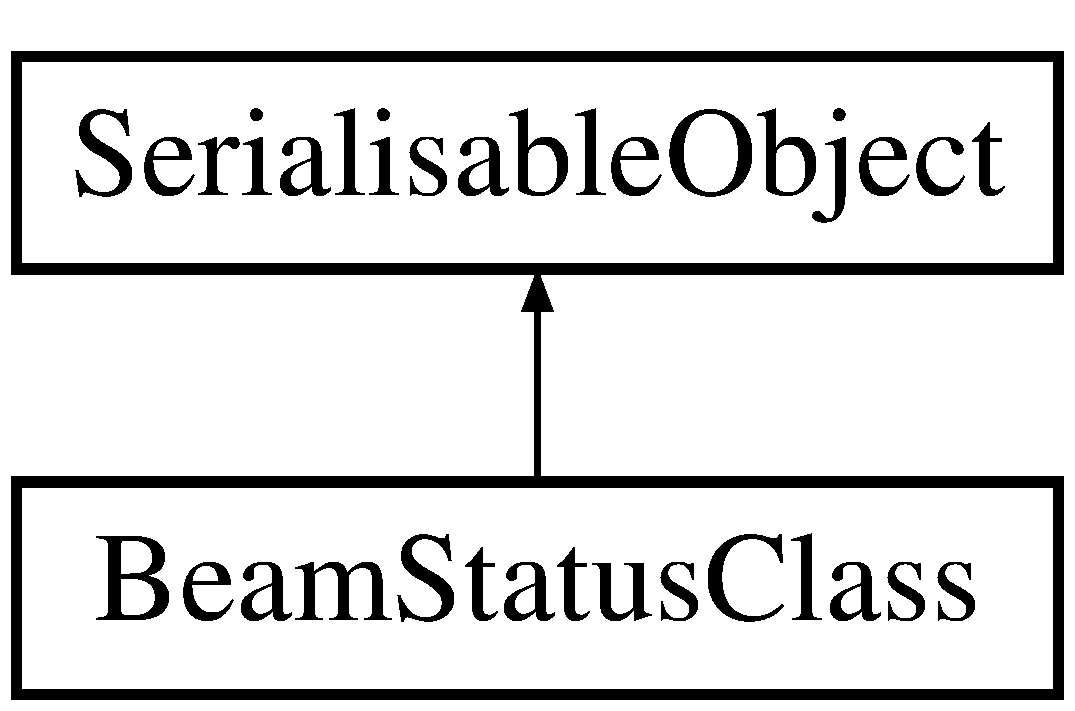
\includegraphics[height=2.000000cm]{classBeamStatusClass}
\end{center}
\end{figure}
\subsection*{Public Member Functions}
\begin{DoxyCompactItemize}
\item 
\hypertarget{classBeamStatusClass_a16f64e35b4c0c7fb4565b930393cf0dc}{{\bfseries Beam\-Status\-Class} (\hyperlink{classTimeClass}{Time\-Class} ts, double beaminten, double beampow, std\-::string beamstab)}\label{classBeamStatusClass_a16f64e35b4c0c7fb4565b930393cf0dc}

\item 
\hypertarget{classBeamStatusClass_a3099faed7d12197a62ee27dacee0d32d}{\hyperlink{classTimeClass}{Time\-Class} {\bfseries Get\-Timestamp} ()}\label{classBeamStatusClass_a3099faed7d12197a62ee27dacee0d32d}

\item 
\hypertarget{classBeamStatusClass_aee60c7ca2561a801cb80d6c239ca2189}{double {\bfseries Get\-Intensity} ()}\label{classBeamStatusClass_aee60c7ca2561a801cb80d6c239ca2189}

\item 
\hypertarget{classBeamStatusClass_abf408e07c997e60b084dc613d5fda75c}{double {\bfseries Get\-Power} ()}\label{classBeamStatusClass_abf408e07c997e60b084dc613d5fda75c}

\item 
\hypertarget{classBeamStatusClass_a052d6ca339a0ca531de200a6cb790fad}{std\-::string {\bfseries Get\-Stability} ()}\label{classBeamStatusClass_a052d6ca339a0ca531de200a6cb790fad}

\item 
\hypertarget{classBeamStatusClass_a26f08683ffd71565d38714886b130459}{void {\bfseries Set\-Timestamp} (\hyperlink{classTimeClass}{Time\-Class} Timestamp\-In)}\label{classBeamStatusClass_a26f08683ffd71565d38714886b130459}

\item 
\hypertarget{classBeamStatusClass_a6ad6d7fe6847a45a043115f6b452ce4a}{void {\bfseries Set\-Intensity} (double Intensity\-In)}\label{classBeamStatusClass_a6ad6d7fe6847a45a043115f6b452ce4a}

\item 
\hypertarget{classBeamStatusClass_a93db8cf0576994acb051c0c17d714e13}{void {\bfseries Set\-Power} (double Power\-In)}\label{classBeamStatusClass_a93db8cf0576994acb051c0c17d714e13}

\item 
\hypertarget{classBeamStatusClass_a4bae86f8f8d6ab9b74dbe73f456a97c6}{void {\bfseries Set\-Stability} (std\-::string Stability\-In)}\label{classBeamStatusClass_a4bae86f8f8d6ab9b74dbe73f456a97c6}

\item 
\hypertarget{classBeamStatusClass_a5a45cde713baaa1d205b0311c7a3ec23}{bool {\bfseries Print} ()}\label{classBeamStatusClass_a5a45cde713baaa1d205b0311c7a3ec23}

\item 
\hypertarget{classBeamStatusClass_a8b86d3c481eab24e6c8a2fda5940d7d8}{void {\bfseries Clear} ()}\label{classBeamStatusClass_a8b86d3c481eab24e6c8a2fda5940d7d8}

\end{DoxyCompactItemize}
\subsection*{Friends}
\begin{DoxyCompactItemize}
\item 
\hypertarget{classBeamStatusClass_ac98d07dd8f7b70e16ccb9a01abf56b9c}{class {\bfseries boost\-::serialization\-::access}}\label{classBeamStatusClass_ac98d07dd8f7b70e16ccb9a01abf56b9c}

\end{DoxyCompactItemize}


The documentation for this class was generated from the following file\-:\begin{DoxyCompactItemize}
\item 
Data\-Model/Beam\-Status\-Class.\-h\end{DoxyCompactItemize}

\hypertarget{classBeamTimeAna}{
\section{BeamTimeAna Class Reference}
\label{classBeamTimeAna}\index{BeamTimeAna@{BeamTimeAna}}
}
\subsection*{Public Member Functions}
\begin{DoxyCompactItemize}
\item 
\hypertarget{classBeamTimeAna_ac5cfa1bfcae38f8b06e35165c34bc7a1}{
bool {\bfseries Initialise} (std::string configfile, \hyperlink{classDataModel}{DataModel} \&data)}
\label{classBeamTimeAna_ac5cfa1bfcae38f8b06e35165c34bc7a1}

\item 
\hypertarget{classBeamTimeAna_a7b308e1c38e71d712f86134f32d6f608}{
bool {\bfseries Execute} ()}
\label{classBeamTimeAna_a7b308e1c38e71d712f86134f32d6f608}

\item 
\hypertarget{classBeamTimeAna_a6327c7597f973dc8d379bab637d49158}{
bool {\bfseries Finalise} ()}
\label{classBeamTimeAna_a6327c7597f973dc8d379bab637d49158}

\item 
\hypertarget{classBeamTimeAna_a7371db48a169030dc1f3c4aef1d2118f}{
vector$<$ double $>$ {\bfseries Transit} (double x0, double y0, double z0, double xslope, double yslope, double baseline, double radius)}
\label{classBeamTimeAna_a7371db48a169030dc1f3c4aef1d2118f}

\end{DoxyCompactItemize}
\subsection*{Public Attributes}
\begin{DoxyCompactItemize}
\item 
\hypertarget{classBeamTimeAna_ab54934df684d5d4710b12eda9f0aa673}{
TH1D $\ast$ {\bfseries hntp}}
\label{classBeamTimeAna_ab54934df684d5d4710b12eda9f0aa673}

\item 
\hypertarget{classBeamTimeAna_a5faa850b2c2878a9b775ce3f4c709b42}{
TH1D $\ast$ {\bfseries hbt}}
\label{classBeamTimeAna_a5faa850b2c2878a9b775ce3f4c709b42}

\item 
\hypertarget{classBeamTimeAna_ab2dd35961bb27797a4611ec1b2893a6d}{
TH1D $\ast$ {\bfseries hbE0}}
\label{classBeamTimeAna_ab2dd35961bb27797a4611ec1b2893a6d}

\item 
\hypertarget{classBeamTimeAna_a6f771c25678b8227977259efd4885b55}{
TH1D $\ast$ {\bfseries hbE\_\-early}}
\label{classBeamTimeAna_a6f771c25678b8227977259efd4885b55}

\item 
\hypertarget{classBeamTimeAna_a9023b54b5567808d2255d05dd77914b9}{
TH1D $\ast$ {\bfseries hbE\_\-med}}
\label{classBeamTimeAna_a9023b54b5567808d2255d05dd77914b9}

\item 
\hypertarget{classBeamTimeAna_aa0db44ef40c14157b9722df4cb1fb200}{
TH1D $\ast$ {\bfseries hbE\_\-late}}
\label{classBeamTimeAna_aa0db44ef40c14157b9722df4cb1fb200}

\item 
\hypertarget{classBeamTimeAna_a19dc31c89cc2c1b4a80631fda8a8c363}{
TH1D $\ast$ {\bfseries hbz0}}
\label{classBeamTimeAna_a19dc31c89cc2c1b4a80631fda8a8c363}

\item 
\hypertarget{classBeamTimeAna_a4634c0e3b22b118c1254f59549046845}{
TH1D $\ast$ {\bfseries hbbaseline}}
\label{classBeamTimeAna_a4634c0e3b22b118c1254f59549046845}

\item 
\hypertarget{classBeamTimeAna_a727d2211d84e0683c805a7d98f0abc0a}{
TH2D $\ast$ {\bfseries hbdvstimecorr}}
\label{classBeamTimeAna_a727d2211d84e0683c805a7d98f0abc0a}

\item 
\hypertarget{classBeamTimeAna_af380e062647bdae7529b0d3f91c5a81d}{
TString {\bfseries InFile}}
\label{classBeamTimeAna_af380e062647bdae7529b0d3f91c5a81d}

\item 
\hypertarget{classBeamTimeAna_a4d2aeab4e93fc15010e6fd1bf56edcdb}{
TString {\bfseries OutFile}}
\label{classBeamTimeAna_a4d2aeab4e93fc15010e6fd1bf56edcdb}

\item 
\hypertarget{classBeamTimeAna_aaf94fd2c4bae8719cb3e40a467d427cd}{
double {\bfseries targetR}}
\label{classBeamTimeAna_aaf94fd2c4bae8719cb3e40a467d427cd}

\item 
\hypertarget{classBeamTimeAna_a0df7b44ed1be5e0f23c6384dc09b01ca}{
double {\bfseries baseline}}
\label{classBeamTimeAna_a0df7b44ed1be5e0f23c6384dc09b01ca}

\item 
\hypertarget{classBeamTimeAna_ac21d70b3320574398e3251092f2c7ef5}{
double {\bfseries tc1}}
\label{classBeamTimeAna_ac21d70b3320574398e3251092f2c7ef5}

\item 
\hypertarget{classBeamTimeAna_ac3ff88abf8e308b8fad48bf1a994f530}{
double {\bfseries tc2}}
\label{classBeamTimeAna_ac3ff88abf8e308b8fad48bf1a994f530}

\item 
\hypertarget{classBeamTimeAna_a64a9f3610a0412a83b6f090e1622ef79}{
double {\bfseries tc3}}
\label{classBeamTimeAna_a64a9f3610a0412a83b6f090e1622ef79}

\item 
\hypertarget{classBeamTimeAna_a9fc48b9d0c43a1d696139811d15ba3c7}{
int {\bfseries ientry}}
\label{classBeamTimeAna_a9fc48b9d0c43a1d696139811d15ba3c7}

\end{DoxyCompactItemize}


The documentation for this class was generated from the following files:\begin{DoxyCompactItemize}
\item 
UserTools/BeamTimeAna/BeamTimeAna.h\item 
UserTools/BeamTimeAna/BeamTimeAna.cpp\end{DoxyCompactItemize}

\hypertarget{classBeamTimeTreeMaker}{
\section{BeamTimeTreeMaker Class Reference}
\label{classBeamTimeTreeMaker}\index{BeamTimeTreeMaker@{BeamTimeTreeMaker}}
}
\subsection*{Public Member Functions}
\begin{DoxyCompactItemize}
\item 
\hypertarget{classBeamTimeTreeMaker_ad0ff2ecf3cf282fc854c086f2bd6902e}{
bool {\bfseries Initialise} (std::string configfile, \hyperlink{classDataModel}{DataModel} \&data)}
\label{classBeamTimeTreeMaker_ad0ff2ecf3cf282fc854c086f2bd6902e}

\item 
\hypertarget{classBeamTimeTreeMaker_a9d8457a840bbd05785c6dbad41efc3e9}{
bool {\bfseries Execute} ()}
\label{classBeamTimeTreeMaker_a9d8457a840bbd05785c6dbad41efc3e9}

\item 
\hypertarget{classBeamTimeTreeMaker_aa854478ff70ed002e41ed38e18fe4a25}{
bool {\bfseries Finalise} ()}
\label{classBeamTimeTreeMaker_aa854478ff70ed002e41ed38e18fe4a25}

\end{DoxyCompactItemize}


The documentation for this class was generated from the following files:\begin{DoxyCompactItemize}
\item 
UserTools/BeamTimeTreeMaker/BeamTimeTreeMaker.h\item 
UserTools/BeamTimeTreeMaker/BeamTimeTreeMaker.cpp\end{DoxyCompactItemize}

\hypertarget{classBeamTimeTreeReader}{
\section{BeamTimeTreeReader Class Reference}
\label{classBeamTimeTreeReader}\index{BeamTimeTreeReader@{BeamTimeTreeReader}}
}
\subsection*{Public Member Functions}
\begin{DoxyCompactItemize}
\item 
\hypertarget{classBeamTimeTreeReader_a156a2386c5a9e9a6aab28a4fbf6df659}{
bool {\bfseries Initialise} (std::string configfile, \hyperlink{classDataModel}{DataModel} \&data)}
\label{classBeamTimeTreeReader_a156a2386c5a9e9a6aab28a4fbf6df659}

\item 
\hypertarget{classBeamTimeTreeReader_ae9094c6a47c9baa1a2394c50daa4fdb3}{
bool {\bfseries Execute} ()}
\label{classBeamTimeTreeReader_ae9094c6a47c9baa1a2394c50daa4fdb3}

\item 
\hypertarget{classBeamTimeTreeReader_ad6b505e7513ac9ab5b950cb15095ac79}{
bool {\bfseries Finalise} ()}
\label{classBeamTimeTreeReader_ad6b505e7513ac9ab5b950cb15095ac79}

\end{DoxyCompactItemize}


The documentation for this class was generated from the following files:\begin{DoxyCompactItemize}
\item 
UserTools/BeamTimeTreeReader/BeamTimeTreeReader.h\item 
UserTools/BeamTimeTreeReader/BeamTimeTreeReader.cpp\end{DoxyCompactItemize}

\hypertarget{classCalibratedADCWaveform}{\section{Calibrated\-A\-D\-C\-Waveform$<$ T $>$ Class Template Reference}
\label{classCalibratedADCWaveform}\index{Calibrated\-A\-D\-C\-Waveform$<$ T $>$@{Calibrated\-A\-D\-C\-Waveform$<$ T $>$}}
}
Inheritance diagram for Calibrated\-A\-D\-C\-Waveform$<$ T $>$\-:\begin{figure}[H]
\begin{center}
\leavevmode
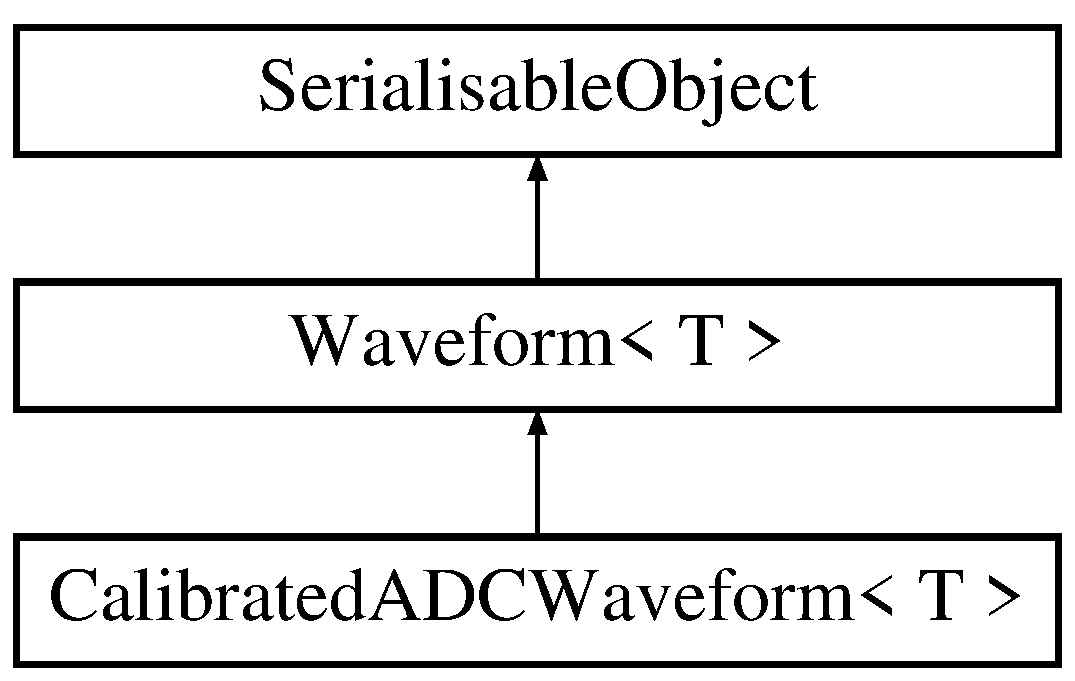
\includegraphics[height=3.000000cm]{classCalibratedADCWaveform}
\end{center}
\end{figure}
\subsection*{Public Member Functions}
\begin{DoxyCompactItemize}
\item 
\hypertarget{classCalibratedADCWaveform_ab8d6abbf935c75db5de184c5a3291ef6}{{\bfseries Calibrated\-A\-D\-C\-Waveform} (const double \&tc, const std\-::vector$<$ T $>$ \&samples, double baseline, double sigma\-\_\-bl)}\label{classCalibratedADCWaveform_ab8d6abbf935c75db5de184c5a3291ef6}

\item 
\hypertarget{classCalibratedADCWaveform_ae22d006546a5666eafd89d361a470798}{double {\bfseries Get\-Baseline} () const }\label{classCalibratedADCWaveform_ae22d006546a5666eafd89d361a470798}

\item 
\hypertarget{classCalibratedADCWaveform_a5afc74fd628dd6d70d60378467092e9d}{double {\bfseries Get\-Sigma\-Baseline} () const }\label{classCalibratedADCWaveform_a5afc74fd628dd6d70d60378467092e9d}

\end{DoxyCompactItemize}
\subsection*{Protected Member Functions}
\begin{DoxyCompactItemize}
\item 
\hypertarget{classCalibratedADCWaveform_a0e5e7326913d63237fd12aee9221b269}{{\footnotesize template$<$class Archive $>$ }\\void {\bfseries serialize} (Archive \&ar, const unsigned int version)}\label{classCalibratedADCWaveform_a0e5e7326913d63237fd12aee9221b269}

\end{DoxyCompactItemize}
\subsection*{Protected Attributes}
\begin{DoxyCompactItemize}
\item 
\hypertarget{classCalibratedADCWaveform_a149f3756091ef8101f03db1740db9caf}{double \hyperlink{classCalibratedADCWaveform_a149f3756091ef8101f03db1740db9caf}{f\-Baseline}}\label{classCalibratedADCWaveform_a149f3756091ef8101f03db1740db9caf}

\begin{DoxyCompactList}\small\item\em Estimated baseline (A\-D\-C counts) determined when performing the calibration. \end{DoxyCompactList}\item 
\hypertarget{classCalibratedADCWaveform_afad42e8ea016aa63d12da79d99b9a40c}{double \hyperlink{classCalibratedADCWaveform_afad42e8ea016aa63d12da79d99b9a40c}{f\-Sigma\-Baseline}}\label{classCalibratedADCWaveform_afad42e8ea016aa63d12da79d99b9a40c}

\begin{DoxyCompactList}\small\item\em Uncertainty (standard deviation) of the estimated baseline (A\-D\-C counts) \end{DoxyCompactList}\end{DoxyCompactItemize}
\subsection*{Friends}
\begin{DoxyCompactItemize}
\item 
\hypertarget{classCalibratedADCWaveform_ac98d07dd8f7b70e16ccb9a01abf56b9c}{class {\bfseries boost\-::serialization\-::access}}\label{classCalibratedADCWaveform_ac98d07dd8f7b70e16ccb9a01abf56b9c}

\end{DoxyCompactItemize}


The documentation for this class was generated from the following file\-:\begin{DoxyCompactItemize}
\item 
Data\-Model/Calibrated\-A\-D\-C\-Waveform.\-h\end{DoxyCompactItemize}

\hypertarget{classCardData}{
\section{CardData Class Reference}
\label{classCardData}\index{CardData@{CardData}}
}
\subsection*{Public Member Functions}
\begin{DoxyCompactItemize}
\item 
\hypertarget{classCardData_a77c665bfd5e8b1f17d6b668e888cf9bd}{
void {\bfseries Reset} ()}
\label{classCardData_a77c665bfd5e8b1f17d6b668e888cf9bd}

\end{DoxyCompactItemize}
\subsection*{Public Attributes}
\begin{DoxyCompactItemize}
\item 
\hypertarget{classCardData_a68649c499d7610955e7a9b143142e224}{
uint64\_\-t {\bfseries LastSync}}
\label{classCardData_a68649c499d7610955e7a9b143142e224}

\item 
\hypertarget{classCardData_a4fdf5313faebd27fee17096a31d0e28e}{
int {\bfseries SequenceID}}
\label{classCardData_a4fdf5313faebd27fee17096a31d0e28e}

\item 
\hypertarget{classCardData_a1297c0ccdeb5cb134cef3c92e01a36ed}{
int {\bfseries StartTimeSec}}
\label{classCardData_a1297c0ccdeb5cb134cef3c92e01a36ed}

\item 
\hypertarget{classCardData_af5393836942c9d857039e8b11bac2952}{
int {\bfseries StartTimeNSec}}
\label{classCardData_af5393836942c9d857039e8b11bac2952}

\item 
\hypertarget{classCardData_a7bd1f3c2269b6c7d3f12ffdd59efa1e6}{
uint64\_\-t {\bfseries StartCount}}
\label{classCardData_a7bd1f3c2269b6c7d3f12ffdd59efa1e6}

\item 
\hypertarget{classCardData_a816053ce45a07b8f7a7e5bfd914c51db}{
std::vector$<$ ULong64\_\-t $>$ {\bfseries TriggerCounts}}
\label{classCardData_a816053ce45a07b8f7a7e5bfd914c51db}

\item 
\hypertarget{classCardData_ab44adb08a1c2de7f4d24463325c87934}{
std::vector$<$ UInt\_\-t $>$ {\bfseries Rates}}
\label{classCardData_ab44adb08a1c2de7f4d24463325c87934}

\item 
\hypertarget{classCardData_a36cb9c0f73fcf5eae251e0a2b1b2bd0f}{
int {\bfseries CardID}}
\label{classCardData_a36cb9c0f73fcf5eae251e0a2b1b2bd0f}

\item 
\hypertarget{classCardData_a6307217de93243eb7b0aa9931f02f706}{
int {\bfseries TriggerNumber}}
\label{classCardData_a6307217de93243eb7b0aa9931f02f706}

\item 
\hypertarget{classCardData_a98f397c0dd49007942f5f25c8cbc67f0}{
int {\bfseries Channels}}
\label{classCardData_a98f397c0dd49007942f5f25c8cbc67f0}

\item 
\hypertarget{classCardData_a82c5fd806c6529cf7a9625dc262f9e8d}{
int {\bfseries BufferSize}}
\label{classCardData_a82c5fd806c6529cf7a9625dc262f9e8d}

\item 
\hypertarget{classCardData_abafe428221ab0987ac51bd7312b29d6b}{
int {\bfseries Eventsize}}
\label{classCardData_abafe428221ab0987ac51bd7312b29d6b}

\item 
\hypertarget{classCardData_a3395d60095ef7aeff93cf2d169a34395}{
int {\bfseries FullBufferSize}}
\label{classCardData_a3395d60095ef7aeff93cf2d169a34395}

\item 
\hypertarget{classCardData_a6190a518c1cc009d169a0f94a333576d}{
std::vector$<$ uint16\_\-t $>$ {\bfseries Data}}
\label{classCardData_a6190a518c1cc009d169a0f94a333576d}

\end{DoxyCompactItemize}


The documentation for this class was generated from the following files:\begin{DoxyCompactItemize}
\item 
UserTools/PulseSimulation/CardData.h\item 
UserTools/PulseSimulation/CardData.cpp\end{DoxyCompactItemize}

\hypertarget{classChannel}{
\section{Channel Class Reference}
\label{classChannel}\index{Channel@{Channel}}
}
Inheritance diagram for Channel::\begin{figure}[H]
\begin{center}
\leavevmode
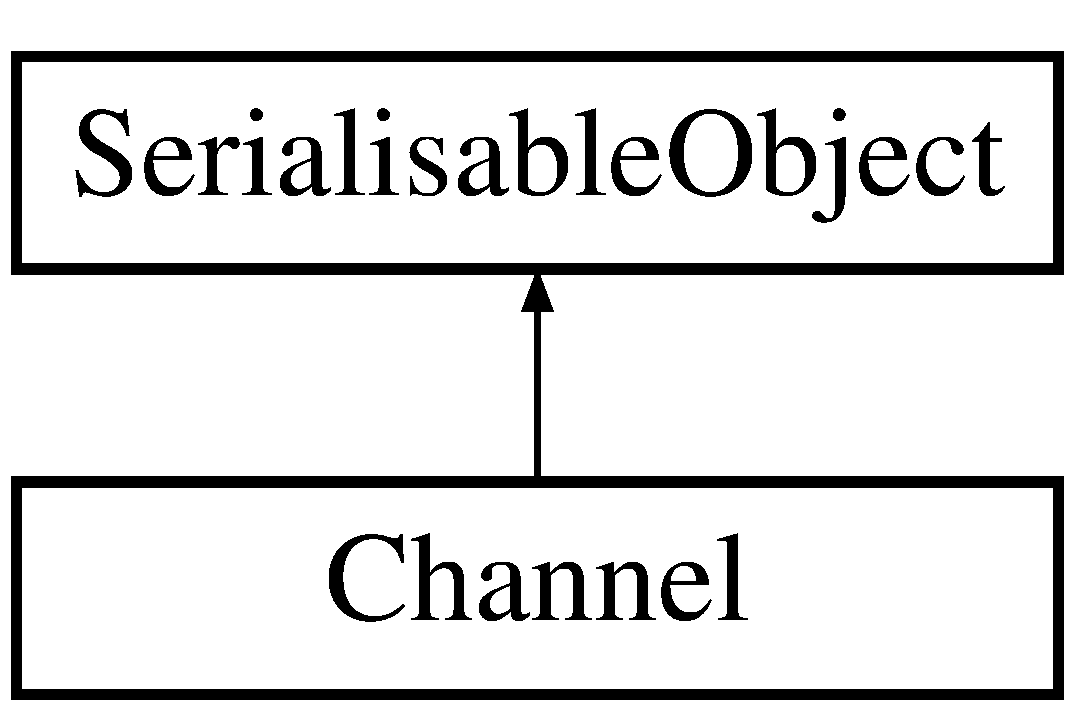
\includegraphics[height=2cm]{classChannel}
\end{center}
\end{figure}
\subsection*{Public Member Functions}
\begin{DoxyCompactItemize}
\item 
\hypertarget{classChannel_ae1078b5c2230dd8fcba2bbd4e8100c57}{
{\bfseries Channel} (unsigned long chnID, \hyperlink{classPosition}{Position} chanpos, int strp, int strpnm, unsigned int sig\_\-crt, unsigned int sig\_\-crd, unsigned int sig\_\-chn, unsigned int lv2\_\-crt, unsigned int lv2\_\-crd, unsigned int lv2\_\-ch, unsigned int hv\_\-crt, unsigned int hv\_\-crd, unsigned int hv\_\-chn, channelstatus chanstat)}
\label{classChannel_ae1078b5c2230dd8fcba2bbd4e8100c57}

\item 
\hypertarget{classChannel_a135981325d6cd967c06b27eef9f0abb0}{
unsigned long {\bfseries GetChannelID} ()}
\label{classChannel_a135981325d6cd967c06b27eef9f0abb0}

\item 
\hypertarget{classChannel_a20f0f3be320a2bb029169a4dbe93cf90}{
\hyperlink{classPosition}{Position} {\bfseries GetChannelPosition} ()}
\label{classChannel_a20f0f3be320a2bb029169a4dbe93cf90}

\item 
\hypertarget{classChannel_aaf73be7554bca0d37886ead17e7dd378}{
int {\bfseries GetStripSide} ()}
\label{classChannel_aaf73be7554bca0d37886ead17e7dd378}

\item 
\hypertarget{classChannel_a8e11f287e50dd85bc16ec31cab5b19f5}{
int {\bfseries GetStripNum} ()}
\label{classChannel_a8e11f287e50dd85bc16ec31cab5b19f5}

\item 
\hypertarget{classChannel_a75f4e595dfd853b4705aaab4b4dd7e5d}{
unsigned int {\bfseries GetSignalCrate} ()}
\label{classChannel_a75f4e595dfd853b4705aaab4b4dd7e5d}

\item 
\hypertarget{classChannel_a3fe69d8eb34bbb71101faa490eff401c}{
unsigned int {\bfseries GetSignalCard} ()}
\label{classChannel_a3fe69d8eb34bbb71101faa490eff401c}

\item 
\hypertarget{classChannel_a0adb3da425cdc8571e3f2070339d1b45}{
unsigned int {\bfseries GetSignalChannel} ()}
\label{classChannel_a0adb3da425cdc8571e3f2070339d1b45}

\item 
\hypertarget{classChannel_aed336de8cbfe7b004a966b08998f10a1}{
unsigned int {\bfseries GetLevel2Crate} ()}
\label{classChannel_aed336de8cbfe7b004a966b08998f10a1}

\item 
\hypertarget{classChannel_a8664e03b00cfb5d9089ffc730ad2db8a}{
unsigned int {\bfseries GetLevel2Card} ()}
\label{classChannel_a8664e03b00cfb5d9089ffc730ad2db8a}

\item 
\hypertarget{classChannel_a3d15a263e8282224e6cac3e39fc537e2}{
unsigned int {\bfseries GetLevel2Channel} ()}
\label{classChannel_a3d15a263e8282224e6cac3e39fc537e2}

\item 
\hypertarget{classChannel_a976eb5f1f568d25d7e6581e947c9026a}{
unsigned int {\bfseries GetHvCrate} ()}
\label{classChannel_a976eb5f1f568d25d7e6581e947c9026a}

\item 
\hypertarget{classChannel_a77afff8e584d72b11c326d503af8cf31}{
unsigned int {\bfseries GetHvCard} ()}
\label{classChannel_a77afff8e584d72b11c326d503af8cf31}

\item 
\hypertarget{classChannel_ab0be6e53cc497a9adfd07d117bd1b8a6}{
unsigned int {\bfseries GetHvChannel} ()}
\label{classChannel_ab0be6e53cc497a9adfd07d117bd1b8a6}

\item 
\hypertarget{classChannel_a0de7daf81b2cf2931ad002365b4e83a7}{
channelstatus {\bfseries GetStatus} ()}
\label{classChannel_a0de7daf81b2cf2931ad002365b4e83a7}

\item 
\hypertarget{classChannel_abc8868d1474907bf055649280aee6ee9}{
void {\bfseries SetChannelID} (unsigned long channelIDin)}
\label{classChannel_abc8868d1474907bf055649280aee6ee9}

\item 
\hypertarget{classChannel_a1ce153da74e56914bfe92f1300d9c4db}{
void {\bfseries SetRelPos} (\hyperlink{classPosition}{Position} pos)}
\label{classChannel_a1ce153da74e56914bfe92f1300d9c4db}

\item 
\hypertarget{classChannel_a2e0a7f64af8639f223be6ae34ee1c866}{
void {\bfseries SetStripSide} (int stripsidein)}
\label{classChannel_a2e0a7f64af8639f223be6ae34ee1c866}

\item 
\hypertarget{classChannel_a1f6b1314cb1db51fd36ed6a734d46af8}{
void {\bfseries SetStripNum} (int stripnumin)}
\label{classChannel_a1f6b1314cb1db51fd36ed6a734d46af8}

\item 
\hypertarget{classChannel_ac7c8bc08322263962606adcee41e5fb9}{
void {\bfseries SetSignalCrate} (unsigned int cratein)}
\label{classChannel_ac7c8bc08322263962606adcee41e5fb9}

\item 
\hypertarget{classChannel_aaa842caa030e691f361bbb38b60c19ac}{
void {\bfseries SetSignalCard} (unsigned int cardin)}
\label{classChannel_aaa842caa030e691f361bbb38b60c19ac}

\item 
\hypertarget{classChannel_acd431f017fca170ea3036f96b0f79e9f}{
void {\bfseries SetSignalChannel} (unsigned int chanin)}
\label{classChannel_acd431f017fca170ea3036f96b0f79e9f}

\item 
\hypertarget{classChannel_a82c97b5b03f81dc4c415f9e6ff4e5cd7}{
void {\bfseries SetLevel2Crate} (unsigned int cratein)}
\label{classChannel_a82c97b5b03f81dc4c415f9e6ff4e5cd7}

\item 
\hypertarget{classChannel_a7144068a386f201f596bb389a09c2806}{
void {\bfseries SetLevel2Card} (unsigned int cardin)}
\label{classChannel_a7144068a386f201f596bb389a09c2806}

\item 
\hypertarget{classChannel_ab6fbf3a0ad9f0a81f57e78b4d0030b1b}{
void {\bfseries SetLevel2Channel} (unsigned int chanin)}
\label{classChannel_ab6fbf3a0ad9f0a81f57e78b4d0030b1b}

\item 
\hypertarget{classChannel_a0fa53863af75dc3113462587216eb72f}{
void {\bfseries SetHvCrate} (unsigned int cratein)}
\label{classChannel_a0fa53863af75dc3113462587216eb72f}

\item 
\hypertarget{classChannel_a6d80a27a7baf8c35f107794f3907cd8f}{
void {\bfseries SetHvCard} (unsigned int cardin)}
\label{classChannel_a6d80a27a7baf8c35f107794f3907cd8f}

\item 
\hypertarget{classChannel_ab710af8a4a2334b2fecb7908ef14f18b}{
void {\bfseries SetHvChannel} (unsigned int chanin)}
\label{classChannel_ab710af8a4a2334b2fecb7908ef14f18b}

\item 
\hypertarget{classChannel_af036686e0a7cecce9996e28cf7f2067f}{
void {\bfseries SetStatus} (channelstatus stat)}
\label{classChannel_af036686e0a7cecce9996e28cf7f2067f}

\item 
\hypertarget{classChannel_a8361bdcaf6dfafc874f6a612dcded25a}{
bool {\bfseries Print} ()}
\label{classChannel_a8361bdcaf6dfafc874f6a612dcded25a}

\item 
\hypertarget{classChannel_ad5ceba06c660386cafaf7801f6adbfad}{
bool {\bfseries PrintStatus} (channelstatus status)}
\label{classChannel_ad5ceba06c660386cafaf7801f6adbfad}

\end{DoxyCompactItemize}
\subsection*{Friends}
\begin{DoxyCompactItemize}
\item 
\hypertarget{classChannel_ac98d07dd8f7b70e16ccb9a01abf56b9c}{
class {\bfseries boost::serialization::access}}
\label{classChannel_ac98d07dd8f7b70e16ccb9a01abf56b9c}

\end{DoxyCompactItemize}


The documentation for this class was generated from the following file:\begin{DoxyCompactItemize}
\item 
DataModel/Channel.h\end{DoxyCompactItemize}

\hypertarget{classChannelKey}{
\section{ChannelKey Class Reference}
\label{classChannelKey}\index{ChannelKey@{ChannelKey}}
}
Inheritance diagram for ChannelKey::\begin{figure}[H]
\begin{center}
\leavevmode
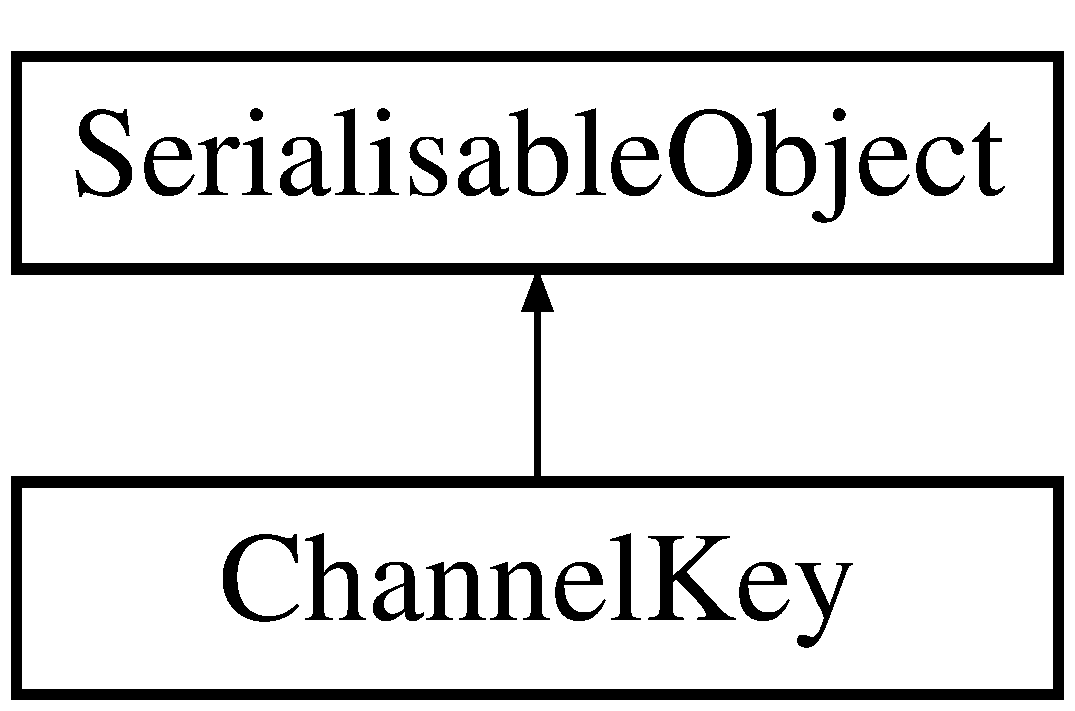
\includegraphics[height=2cm]{classChannelKey}
\end{center}
\end{figure}
\subsection*{Public Member Functions}
\begin{DoxyCompactItemize}
\item 
\hypertarget{classChannelKey_a1b98b5ec38b5a372908869bec5e76885}{
{\bfseries ChannelKey} (subdetector subdetin, uint32\_\-t detelin)}
\label{classChannelKey_a1b98b5ec38b5a372908869bec5e76885}

\item 
\hypertarget{classChannelKey_a5b156478be91e4d58829661e9a63da13}{
subdetector {\bfseries GetSubDetectorType} () const }
\label{classChannelKey_a5b156478be91e4d58829661e9a63da13}

\item 
\hypertarget{classChannelKey_a2788a95997db38d5bf8075da6eb2d50c}{
uint32\_\-t {\bfseries GetDetectorElementIndex} () const }
\label{classChannelKey_a2788a95997db38d5bf8075da6eb2d50c}

\item 
\hypertarget{classChannelKey_a84b468bc66e943e8ad9b4102f8c8446d}{
void {\bfseries SetSubDetectorType} (subdetector subdetin)}
\label{classChannelKey_a84b468bc66e943e8ad9b4102f8c8446d}

\item 
\hypertarget{classChannelKey_a8727334520a49cba3d6a01a6727a361d}{
void {\bfseries SetDetectorElementIndex} (uint32\_\-t detelin)}
\label{classChannelKey_a8727334520a49cba3d6a01a6727a361d}

\item 
\hypertarget{classChannelKey_a7bb14ec44da38dd1152cf7912f7a607d}{
bool {\bfseries Print} ()}
\label{classChannelKey_a7bb14ec44da38dd1152cf7912f7a607d}

\item 
\hypertarget{classChannelKey_abcadfaf457add635aef1ec372e5340d7}{
bool {\bfseries operator$<$} (const \hyperlink{classChannelKey}{ChannelKey} rhs) const }
\label{classChannelKey_abcadfaf457add635aef1ec372e5340d7}

\end{DoxyCompactItemize}
\subsection*{Friends}
\begin{DoxyCompactItemize}
\item 
\hypertarget{classChannelKey_ac98d07dd8f7b70e16ccb9a01abf56b9c}{
class {\bfseries boost::serialization::access}}
\label{classChannelKey_ac98d07dd8f7b70e16ccb9a01abf56b9c}

\end{DoxyCompactItemize}


The documentation for this class was generated from the following file:\begin{DoxyCompactItemize}
\item 
DataModel/ChannelKey.h\end{DoxyCompactItemize}

\hypertarget{classCheckDetectorCounts}{\section{Check\-Detector\-Counts Class Reference}
\label{classCheckDetectorCounts}\index{Check\-Detector\-Counts@{Check\-Detector\-Counts}}
}
Inheritance diagram for Check\-Detector\-Counts\-:\begin{figure}[H]
\begin{center}
\leavevmode
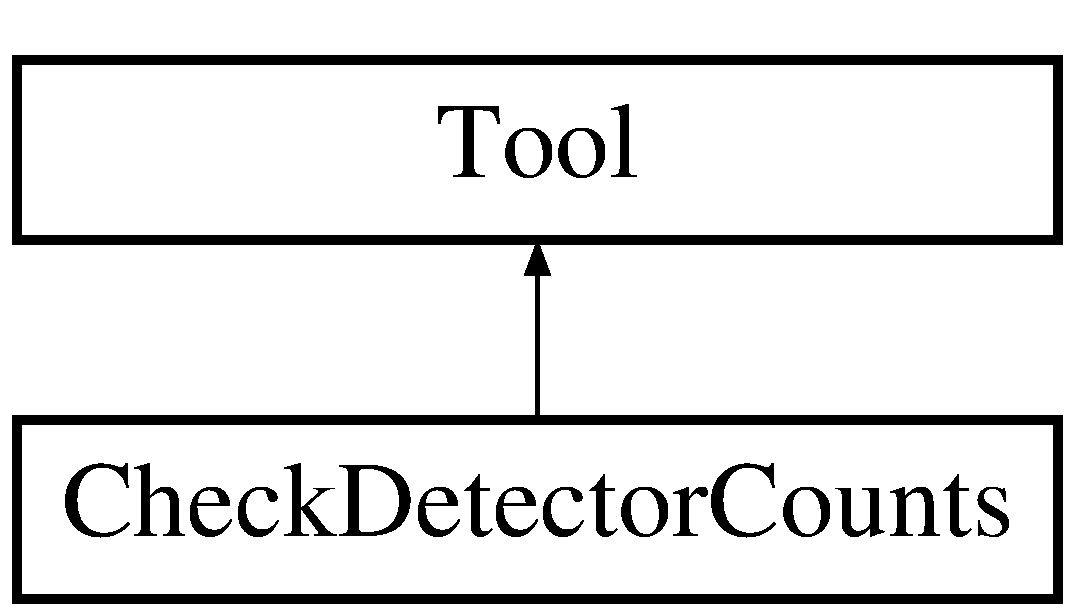
\includegraphics[height=2.000000cm]{classCheckDetectorCounts}
\end{center}
\end{figure}
\subsection*{Public Member Functions}
\begin{DoxyCompactItemize}
\item 
\hypertarget{classCheckDetectorCounts_ac64b90d8952c7d3b1f970c7f7d6180df}{bool {\bfseries Initialise} (std\-::string configfile, \hyperlink{classDataModel}{Data\-Model} \&data)}\label{classCheckDetectorCounts_ac64b90d8952c7d3b1f970c7f7d6180df}

\item 
\hypertarget{classCheckDetectorCounts_a5e10b7af8ac4184d2cfc695b47e5c23d}{bool {\bfseries Execute} ()}\label{classCheckDetectorCounts_a5e10b7af8ac4184d2cfc695b47e5c23d}

\item 
\hypertarget{classCheckDetectorCounts_a7fb977a13d93552a7e7feefd9a419125}{bool {\bfseries Finalise} ()}\label{classCheckDetectorCounts_a7fb977a13d93552a7e7feefd9a419125}

\end{DoxyCompactItemize}


The documentation for this class was generated from the following files\-:\begin{DoxyCompactItemize}
\item 
User\-Tools/\-Check\-Detector\-Counts/Check\-Detector\-Counts.\-h\item 
User\-Tools/\-Check\-Detector\-Counts/Check\-Detector\-Counts.\-cpp\end{DoxyCompactItemize}

\hypertarget{classDataModel}{\section{Data\-Model Class Reference}
\label{classDataModel}\index{Data\-Model@{Data\-Model}}
}


{\ttfamily \#include $<$Data\-Model.\-h$>$}

\subsection*{Public Member Functions}
\begin{DoxyCompactItemize}
\item 
\hypertarget{classDataModel_abff03aef2cb531142a35781bb87c3365}{\hyperlink{classDataModel_abff03aef2cb531142a35781bb87c3365}{Data\-Model} ()}\label{classDataModel_abff03aef2cb531142a35781bb87c3365}

\begin{DoxyCompactList}\small\item\em Simple constructor. \end{DoxyCompactList}\end{DoxyCompactItemize}
\subsection*{Public Attributes}
\begin{DoxyCompactItemize}
\item 
\hypertarget{classDataModel_a4baac5fe364a7a23762d70d2c2216486}{Store \hyperlink{classDataModel_a4baac5fe364a7a23762d70d2c2216486}{vars}}\label{classDataModel_a4baac5fe364a7a23762d70d2c2216486}

\begin{DoxyCompactList}\small\item\em This Store can be used for any variables. It is an inefficent ascii based storage. \end{DoxyCompactList}\item 
\hypertarget{classDataModel_a878e0d87285f0b3541a3e7116a5f00b6}{Boost\-Store \hyperlink{classDataModel_a878e0d87285f0b3541a3e7116a5f00b6}{C\-Store}}\label{classDataModel_a878e0d87285f0b3541a3e7116a5f00b6}

\begin{DoxyCompactList}\small\item\em This is a more efficent binary Boost\-Store that can be used to store a dynamic set of inter Tool variables. \end{DoxyCompactList}\item 
\hypertarget{classDataModel_ad1ffc080c3b263bf3ee382a531321ad4}{std\-::map$<$ std\-::string, \\*
Boost\-Store $\ast$ $>$ \hyperlink{classDataModel_ad1ffc080c3b263bf3ee382a531321ad4}{Stores}}\label{classDataModel_ad1ffc080c3b263bf3ee382a531321ad4}

\begin{DoxyCompactList}\small\item\em This is a map of named Boo\-Store pointers which can be deffined to hold a nammed collection of any tipe of Boost\-Store. It is usefull to store data that needs subdividing into differnt stores. \end{DoxyCompactList}\item 
\hypertarget{classDataModel_aa777da4c632e4659ee5b1447ad513458}{Logging $\ast$ \hyperlink{classDataModel_aa777da4c632e4659ee5b1447ad513458}{Log}}\label{classDataModel_aa777da4c632e4659ee5b1447ad513458}

\begin{DoxyCompactList}\small\item\em Log class pointer for use in Tools, it can be used to send messages which can have multiple error levels and destination end points. \end{DoxyCompactList}\item 
\hypertarget{classDataModel_a2c6dfd692e50f90e55338970ea7f8d61}{zmq\-::context\-\_\-t $\ast$ \hyperlink{classDataModel_a2c6dfd692e50f90e55338970ea7f8d61}{context}}\label{classDataModel_a2c6dfd692e50f90e55338970ea7f8d61}

\begin{DoxyCompactList}\small\item\em Z\-M\-Q contex used for producing zmq sockets for inter thread, process, or computer communication. \end{DoxyCompactList}\end{DoxyCompactItemize}


\subsection{Detailed Description}
This class Is a transient data model class for your Tools within the Tool\-Chain. If Tools need to comunicate they pass all data objects through the data model. There fore inter tool data objects should be deffined in this class.

\begin{DoxyParagraph}{Author\-:}
B.\-Richards 
\end{DoxyParagraph}
\begin{DoxyParagraph}{Date\-:}
2019/05/26 18\-:34\-:00 
\end{DoxyParagraph}
Contact\-: \href{mailto:b.richards@qmul.ac.uk}{\tt b.\-richards@qmul.\-ac.\-uk} 

The documentation for this class was generated from the following files\-:\begin{DoxyCompactItemize}
\item 
Data\-Model/Data\-Model.\-h\item 
Data\-Model/Data\-Model.\-cpp\end{DoxyCompactItemize}

\hypertarget{classDetector}{
\section{Detector Class Reference}
\label{classDetector}\index{Detector@{Detector}}
}
Inheritance diagram for Detector::\begin{figure}[H]
\begin{center}
\leavevmode
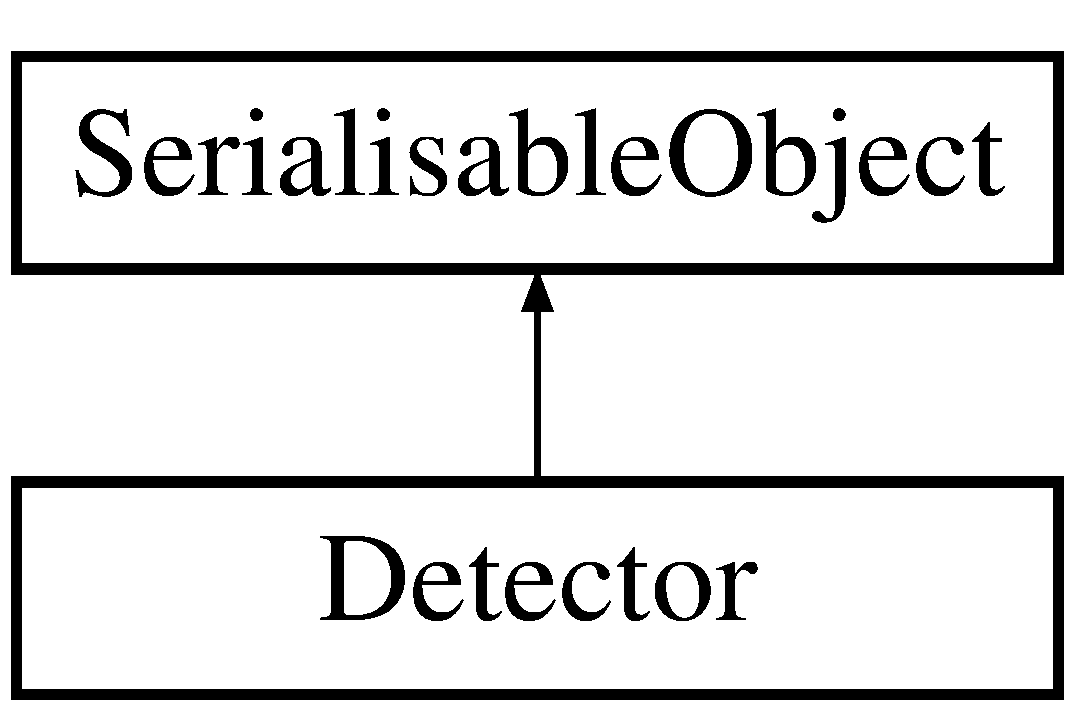
\includegraphics[height=2cm]{classDetector}
\end{center}
\end{figure}
\subsection*{Public Member Functions}
\begin{DoxyCompactItemize}
\item 
\hypertarget{classDetector_acc63b0828ae0a8fecca2f71b26f14531}{
{\bfseries Detector} (int detid, std::string DetEle, std::string CylLoc, \hyperlink{classPosition}{Position} posin, \hyperlink{classDirection}{Direction} dirin, std::string detype, detectorstatus stat, double avgrate, map$<$ unsigned long, \hyperlink{classChannel}{Channel} $>$ channelsin=\{\})}
\label{classDetector_acc63b0828ae0a8fecca2f71b26f14531}

\item 
\hypertarget{classDetector_a7622dcc0d32a77b2d81f3346f9d486a6}{
std::string {\bfseries GetDetectorElement} ()}
\label{classDetector_a7622dcc0d32a77b2d81f3346f9d486a6}

\item 
\hypertarget{classDetector_ae706947ab25223c2707b0b04fa1cf999}{
\hyperlink{classPosition}{Position} {\bfseries GetDetectorPosition} ()}
\label{classDetector_ae706947ab25223c2707b0b04fa1cf999}

\item 
\hypertarget{classDetector_ace3843de946676dac6a031ab21ab2537}{
\hyperlink{classPosition}{Position} {\bfseries GetPositionInTank} ()}
\label{classDetector_ace3843de946676dac6a031ab21ab2537}

\item 
\hypertarget{classDetector_a80cbd9a7402579d601953a91d6883a94}{
\hyperlink{classDirection}{Direction} {\bfseries GetDetectorDirection} ()}
\label{classDetector_a80cbd9a7402579d601953a91d6883a94}

\item 
\hypertarget{classDetector_a85412b023bb48b28e27c9b308857653f}{
int {\bfseries GetDetectorID} ()}
\label{classDetector_a85412b023bb48b28e27c9b308857653f}

\item 
\hypertarget{classDetector_a0f5e4f78e6e64903f46679577609a320}{
std::string {\bfseries GetDetectorType} ()}
\label{classDetector_a0f5e4f78e6e64903f46679577609a320}

\item 
\hypertarget{classDetector_adf81db079151a065407d44558a6240b3}{
detectorstatus {\bfseries GetStatus} ()}
\label{classDetector_adf81db079151a065407d44558a6240b3}

\item 
\hypertarget{classDetector_a1aa42e2f99fd99f2b09d2ab0a1ff4405}{
std::map$<$ unsigned long, \hyperlink{classChannel}{Channel} $>$ $\ast$ {\bfseries GetChannels} ()}
\label{classDetector_a1aa42e2f99fd99f2b09d2ab0a1ff4405}

\item 
\hypertarget{classDetector_adc95528c7b20269f2f30a6d5330a7fd7}{
void {\bfseries AddChannel} (\hyperlink{classChannel}{Channel} chanin)}
\label{classDetector_adc95528c7b20269f2f30a6d5330a7fd7}

\item 
\hypertarget{classDetector_aa87b945be097376ed4d9e7ad11da60f5}{
std::string {\bfseries GetTankLocation} ()}
\label{classDetector_aa87b945be097376ed4d9e7ad11da60f5}

\item 
\hypertarget{classDetector_ac0b5f82030923f555f4420c110de97b0}{
\hyperlink{classGeometry}{Geometry} $\ast$ {\bfseries GetGeometryPtr} ()}
\label{classDetector_ac0b5f82030923f555f4420c110de97b0}

\item 
\hypertarget{classDetector_a5a447c98e1cda4bcb669d6f0cf7f372e}{
void {\bfseries SetDetectorElement} (std::string DetEleIn)}
\label{classDetector_a5a447c98e1cda4bcb669d6f0cf7f372e}

\item 
\hypertarget{classDetector_a388c07e8a741d22a5dcec27ae0718223}{
void {\bfseries SetDetectorPosition} (\hyperlink{classPosition}{Position} DetectorPositionIn)}
\label{classDetector_a388c07e8a741d22a5dcec27ae0718223}

\item 
\hypertarget{classDetector_a349a08c4b6eb90415971d798f6c35466}{
void {\bfseries SetDetectorDirection} (\hyperlink{classDirection}{Direction} DetectorDirectionIn)}
\label{classDetector_a349a08c4b6eb90415971d798f6c35466}

\item 
\hypertarget{classDetector_ac6b4e26f7391b0e96cddf047aec6baf3}{
void {\bfseries SetDetectorID} (int DetectorIDIn)}
\label{classDetector_ac6b4e26f7391b0e96cddf047aec6baf3}

\item 
\hypertarget{classDetector_ac903797b8948e0107de513de60757b2e}{
void {\bfseries SetDetectorType} (std::string DetectorTypeIn)}
\label{classDetector_ac903797b8948e0107de513de60757b2e}

\item 
\hypertarget{classDetector_a912c695a5b4c7bdac1fd6d408cb4e943}{
void {\bfseries SetStatus} (detectorstatus StatusIn)}
\label{classDetector_a912c695a5b4c7bdac1fd6d408cb4e943}

\item 
\hypertarget{classDetector_acc18123ffd61248f94f86eae4a54a0af}{
void {\bfseries SetTankLocation} (std::string locin)}
\label{classDetector_acc18123ffd61248f94f86eae4a54a0af}

\item 
\hypertarget{classDetector_a314120e55ef11500f7e0463e94ae37bb}{
void {\bfseries SetGeometryPtr} (\hyperlink{classGeometry}{Geometry} $\ast$geomin)}
\label{classDetector_a314120e55ef11500f7e0463e94ae37bb}

\item 
\hypertarget{classDetector_a89a77c0af830a448ab599e9cfce4a2d8}{
bool {\bfseries Print} ()}
\label{classDetector_a89a77c0af830a448ab599e9cfce4a2d8}

\item 
\hypertarget{classDetector_a4fced6fd118fe1371ee7e7193c666710}{
bool {\bfseries PrintStatus} (detectorstatus status)}
\label{classDetector_a4fced6fd118fe1371ee7e7193c666710}

\item 
\hypertarget{classDetector_af25e30e52b653b1380743676322f88ea}{
void {\bfseries PrintChannels} ()}
\label{classDetector_af25e30e52b653b1380743676322f88ea}

\end{DoxyCompactItemize}
\subsection*{Friends}
\begin{DoxyCompactItemize}
\item 
\hypertarget{classDetector_ac98d07dd8f7b70e16ccb9a01abf56b9c}{
class {\bfseries boost::serialization::access}}
\label{classDetector_ac98d07dd8f7b70e16ccb9a01abf56b9c}

\end{DoxyCompactItemize}


The documentation for this class was generated from the following files:\begin{DoxyCompactItemize}
\item 
DataModel/Detector.h\item 
DataModel/Detector.cpp\end{DoxyCompactItemize}

\hypertarget{classDigitBuilder}{\section{Digit\-Builder Class Reference}
\label{classDigitBuilder}\index{Digit\-Builder@{Digit\-Builder}}
}


{\ttfamily \#include $<$Digit\-Builder.\-h$>$}

Inheritance diagram for Digit\-Builder\-:\begin{figure}[H]
\begin{center}
\leavevmode
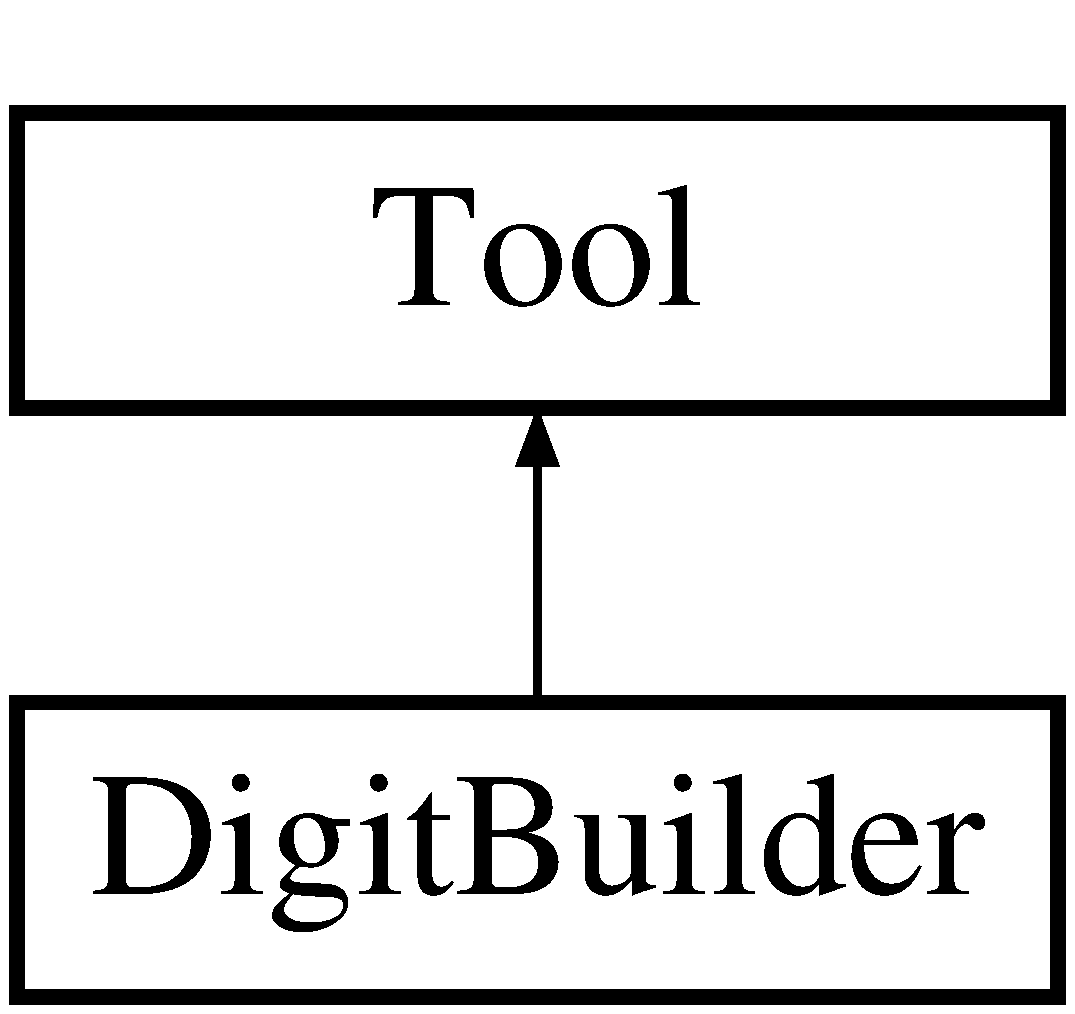
\includegraphics[height=2.000000cm]{classDigitBuilder}
\end{center}
\end{figure}
\subsection*{Public Member Functions}
\begin{DoxyCompactItemize}
\item 
bool \hyperlink{classDigitBuilder_aacb1cb36e5063ba4774381012ac148d6}{Initialise} (std\-::string configfile, \hyperlink{classDataModel}{Data\-Model} \&data)
\item 
bool \hyperlink{classDigitBuilder_a77c2d2d5208563e7a9d8f1a2c8a4777c}{Execute} ()
\item 
\hypertarget{classDigitBuilder_adfbdd3e33b7ac69a7be4bf54fd264066}{bool {\bfseries Finalise} ()}\label{classDigitBuilder_adfbdd3e33b7ac69a7be4bf54fd264066}

\end{DoxyCompactItemize}
\subsection*{Static Public Member Functions}
\begin{DoxyCompactItemize}
\item 
\hypertarget{classDigitBuilder_a3bffe9fa6444a64595122c859d00513d}{static \hyperlink{classDigitBuilder}{Digit\-Builder} $\ast$ {\bfseries Instance} ()}\label{classDigitBuilder_a3bffe9fa6444a64595122c859d00513d}

\end{DoxyCompactItemize}


\subsection{Detailed Description}
This tool reads the raw data from the file and creates a \hyperlink{classDigitBuilder}{Digit\-Builder} object Jingbo Wang \href{mailto:jiowang@ucdavis.edu}{\tt jiowang@ucdavis.\-edu} 

\subsection{Member Function Documentation}
\hypertarget{classDigitBuilder_a77c2d2d5208563e7a9d8f1a2c8a4777c}{\index{Digit\-Builder@{Digit\-Builder}!Execute@{Execute}}
\index{Execute@{Execute}!DigitBuilder@{Digit\-Builder}}
\subsubsection[{Execute}]{\setlength{\rightskip}{0pt plus 5cm}bool Digit\-Builder\-::\-Execute (
\begin{DoxyParamCaption}
{}
\end{DoxyParamCaption}
)}}\label{classDigitBuilder_a77c2d2d5208563e7a9d8f1a2c8a4777c}
Reset everything

see if \char`\"{}\-Reco\-Event\char`\"{} exists. If not, make it

Retrieve necessary info from A\-N\-N\-I\-E\-Event

Build \hyperlink{classRecoDigit}{Reco\-Digit}

\hyperlink{classHit}{Hit} info. to Reco\-Event \hypertarget{classDigitBuilder_aacb1cb36e5063ba4774381012ac148d6}{\index{Digit\-Builder@{Digit\-Builder}!Initialise@{Initialise}}
\index{Initialise@{Initialise}!DigitBuilder@{Digit\-Builder}}
\subsubsection[{Initialise}]{\setlength{\rightskip}{0pt plus 5cm}bool Digit\-Builder\-::\-Initialise (
\begin{DoxyParamCaption}
\item[{std\-::string}]{configfile, }
\item[{{\bf Data\-Model} \&}]{data}
\end{DoxyParamCaption}
)}}\label{classDigitBuilder_aacb1cb36e5063ba4774381012ac148d6}
Get the Tool configuration variables

Construct the other objects we'll be setting at event level, 

The documentation for this class was generated from the following files\-:\begin{DoxyCompactItemize}
\item 
User\-Tools/\-Digit\-Builder/Digit\-Builder.\-h\item 
User\-Tools/\-Digit\-Builder/Digit\-Builder.\-cpp\end{DoxyCompactItemize}

\hypertarget{classDigitBuilderDoE}{
\section{DigitBuilderDoE Class Reference}
\label{classDigitBuilderDoE}\index{DigitBuilderDoE@{DigitBuilderDoE}}
}
\subsection*{Public Member Functions}
\begin{DoxyCompactItemize}
\item 
bool \hyperlink{classDigitBuilderDoE_a629487cb173c306f7796d4466049d790}{Initialise} (std::string configfile, \hyperlink{classDataModel}{DataModel} \&data)
\item 
bool \hyperlink{classDigitBuilderDoE_abbf2b8912d5a5e01c8755ad873e99520}{Execute} ()
\item 
\hypertarget{classDigitBuilderDoE_ad51a7fbe29242cd5f5283a0e1a488798}{
bool {\bfseries Finalise} ()}
\label{classDigitBuilderDoE_ad51a7fbe29242cd5f5283a0e1a488798}

\end{DoxyCompactItemize}
\subsection*{Static Public Member Functions}
\begin{DoxyCompactItemize}
\item 
\hypertarget{classDigitBuilderDoE_ae6f5d12e2b1c6a3a57097ab946add570}{
static \hyperlink{classDigitBuilderDoE}{DigitBuilderDoE} $\ast$ {\bfseries Instance} ()}
\label{classDigitBuilderDoE_ae6f5d12e2b1c6a3a57097ab946add570}

\end{DoxyCompactItemize}


\subsection{Member Function Documentation}
\hypertarget{classDigitBuilderDoE_abbf2b8912d5a5e01c8755ad873e99520}{
\index{DigitBuilderDoE@{DigitBuilderDoE}!Execute@{Execute}}
\index{Execute@{Execute}!DigitBuilderDoE@{DigitBuilderDoE}}
\subsubsection[{Execute}]{\setlength{\rightskip}{0pt plus 5cm}bool DigitBuilderDoE::Execute ()}}
\label{classDigitBuilderDoE_abbf2b8912d5a5e01c8755ad873e99520}


see if \char`\"{}RecoEvent\char`\"{} exists

Push recodigits and muon truth info to RecoEvent \hypertarget{classDigitBuilderDoE_a629487cb173c306f7796d4466049d790}{
\index{DigitBuilderDoE@{DigitBuilderDoE}!Initialise@{Initialise}}
\index{Initialise@{Initialise}!DigitBuilderDoE@{DigitBuilderDoE}}
\subsubsection[{Initialise}]{\setlength{\rightskip}{0pt plus 5cm}bool DigitBuilderDoE::Initialise (std::string {\em configfile}, \/  {\bf DataModel} \& {\em data})}}
\label{classDigitBuilderDoE_a629487cb173c306f7796d4466049d790}


Construct the other objects we'll be setting at event level, 

The documentation for this class was generated from the following files:\begin{DoxyCompactItemize}
\item 
UserTools/DigitBuilderDoE/DigitBuilderDoE.h\item 
UserTools/DigitBuilderDoE/DigitBuilderDoE.cpp\end{DoxyCompactItemize}

\hypertarget{classDigitBuilderROOT}{
\section{DigitBuilderROOT Class Reference}
\label{classDigitBuilderROOT}\index{DigitBuilderROOT@{DigitBuilderROOT}}
}
\subsection*{Public Member Functions}
\begin{DoxyCompactItemize}
\item 
\hypertarget{classDigitBuilderROOT_a7ab06541c442a8bc03adc0c7a4b32086}{
bool {\bfseries Initialise} (std::string configfile, \hyperlink{classDataModel}{DataModel} \&data)}
\label{classDigitBuilderROOT_a7ab06541c442a8bc03adc0c7a4b32086}

\item 
\hypertarget{classDigitBuilderROOT_a9529acec5b1a6cf468e57c96bf55453d}{
bool {\bfseries Execute} ()}
\label{classDigitBuilderROOT_a9529acec5b1a6cf468e57c96bf55453d}

\item 
\hypertarget{classDigitBuilderROOT_a1beb47fea60dc16f627a339ee0597e71}{
bool {\bfseries Finalise} ()}
\label{classDigitBuilderROOT_a1beb47fea60dc16f627a339ee0597e71}

\item 
\hypertarget{classDigitBuilderROOT_a894cb087ddb66f65fe966d4155b03256}{
void {\bfseries PushTrueVertex} (bool savetodisk)}
\label{classDigitBuilderROOT_a894cb087ddb66f65fe966d4155b03256}

\item 
void \hyperlink{classDigitBuilderROOT_af623aff0f8d4b58cb4c7182da49b76b7}{PushRecoDigits} (bool savetodisk)
\item 
void \hyperlink{classDigitBuilderROOT_a7edde994bef160f405d740b5e9b01176}{PushTrueWaterTrackLength} (double WaterT)
\item 
void \hyperlink{classDigitBuilderROOT_adca0d96fa944b38e44e2ebb8a619f77b}{PushTrueMRDTrackLength} (double MRDT)
\item 
\hypertarget{classDigitBuilderROOT_a01cd5fb15e6ebe304ba751652de2b37b}{
void {\bfseries Reset} ()}
\label{classDigitBuilderROOT_a01cd5fb15e6ebe304ba751652de2b37b}

\end{DoxyCompactItemize}


\subsection{Member Function Documentation}
\hypertarget{classDigitBuilderROOT_af623aff0f8d4b58cb4c7182da49b76b7}{
\index{DigitBuilderROOT@{DigitBuilderROOT}!PushRecoDigits@{PushRecoDigits}}
\index{PushRecoDigits@{PushRecoDigits}!DigitBuilderROOT@{DigitBuilderROOT}}
\subsubsection[{PushRecoDigits}]{\setlength{\rightskip}{0pt plus 5cm}void DigitBuilderROOT::PushRecoDigits (bool {\em savetodisk})}}
\label{classDigitBuilderROOT_af623aff0f8d4b58cb4c7182da49b76b7}


$>$ Add digits to RecoEvent \hypertarget{classDigitBuilderROOT_adca0d96fa944b38e44e2ebb8a619f77b}{
\index{DigitBuilderROOT@{DigitBuilderROOT}!PushTrueMRDTrackLength@{PushTrueMRDTrackLength}}
\index{PushTrueMRDTrackLength@{PushTrueMRDTrackLength}!DigitBuilderROOT@{DigitBuilderROOT}}
\subsubsection[{PushTrueMRDTrackLength}]{\setlength{\rightskip}{0pt plus 5cm}void DigitBuilderROOT::PushTrueMRDTrackLength (double {\em MRDT})}}
\label{classDigitBuilderROOT_adca0d96fa944b38e44e2ebb8a619f77b}


$>$ Add digits to RecoEvent \hypertarget{classDigitBuilderROOT_a7edde994bef160f405d740b5e9b01176}{
\index{DigitBuilderROOT@{DigitBuilderROOT}!PushTrueWaterTrackLength@{PushTrueWaterTrackLength}}
\index{PushTrueWaterTrackLength@{PushTrueWaterTrackLength}!DigitBuilderROOT@{DigitBuilderROOT}}
\subsubsection[{PushTrueWaterTrackLength}]{\setlength{\rightskip}{0pt plus 5cm}void DigitBuilderROOT::PushTrueWaterTrackLength (double {\em WaterT})}}
\label{classDigitBuilderROOT_a7edde994bef160f405d740b5e9b01176}


$>$ Add digits to RecoEvent 

The documentation for this class was generated from the following files:\begin{DoxyCompactItemize}
\item 
UserTools/DigitBuilderROOT/DigitBuilderROOT.h\item 
UserTools/DigitBuilderROOT/DigitBuilderROOT.cpp\end{DoxyCompactItemize}

\hypertarget{classDirection}{\section{Direction Class Reference}
\label{classDirection}\index{Direction@{Direction}}
}
Inheritance diagram for Direction\-:\begin{figure}[H]
\begin{center}
\leavevmode
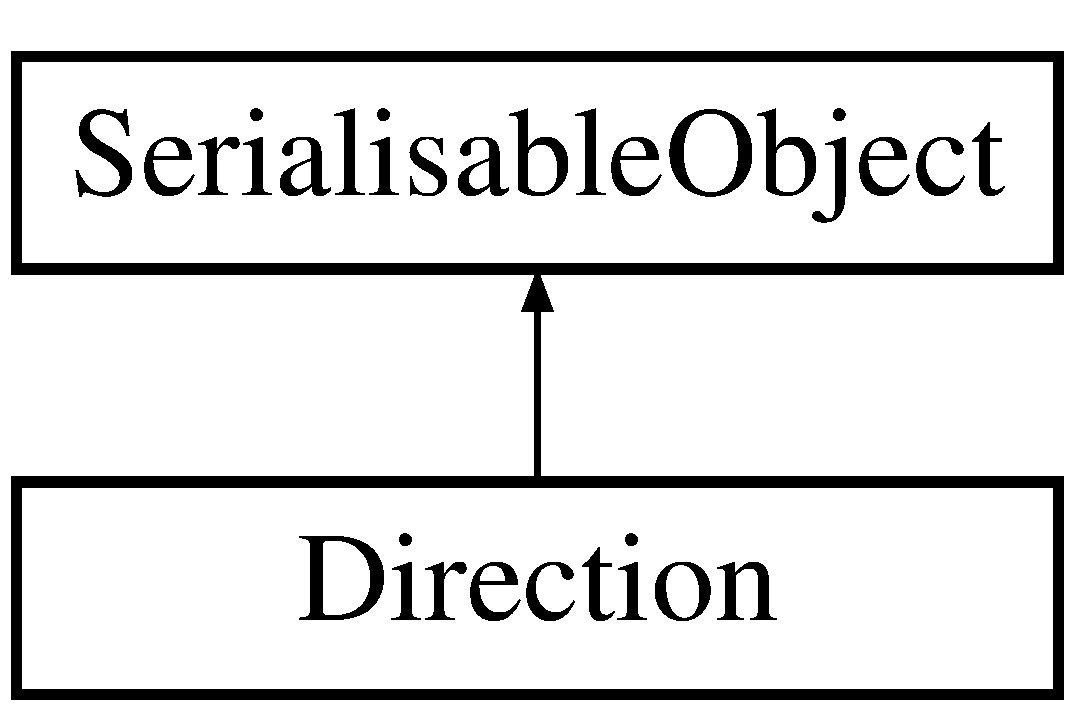
\includegraphics[height=2.000000cm]{classDirection}
\end{center}
\end{figure}
\subsection*{Public Member Functions}
\begin{DoxyCompactItemize}
\item 
\hypertarget{classDirection_a6ab97d45f5cba3aa5e571f0c0e8dd5be}{{\bfseries Direction} (double xin, double yin, double zin)}\label{classDirection_a6ab97d45f5cba3aa5e571f0c0e8dd5be}

\item 
\hypertarget{classDirection_ae577ffea4af24ebc490093c55adbbdba}{{\bfseries Direction} (double phiin, double thetain)}\label{classDirection_ae577ffea4af24ebc490093c55adbbdba}

\item 
\hypertarget{classDirection_a16e35cd86702666a7f2a9de1962b99d3}{double {\bfseries X} () const }\label{classDirection_a16e35cd86702666a7f2a9de1962b99d3}

\item 
\hypertarget{classDirection_a87038a7a2381c3bfa062d1016ece1b0a}{double {\bfseries Y} () const }\label{classDirection_a87038a7a2381c3bfa062d1016ece1b0a}

\item 
\hypertarget{classDirection_a7e8275fe3078f9fb2c4f17cafd219dca}{double {\bfseries Z} () const }\label{classDirection_a7e8275fe3078f9fb2c4f17cafd219dca}

\item 
\hypertarget{classDirection_ae60296b4e458a378de7fac5e194d128a}{double {\bfseries Get\-Phi} () const }\label{classDirection_ae60296b4e458a378de7fac5e194d128a}

\item 
\hypertarget{classDirection_ab10dd98d45f913882643a8ec3a0063a1}{double {\bfseries Get\-Phi\-Deg} () const }\label{classDirection_ab10dd98d45f913882643a8ec3a0063a1}

\item 
\hypertarget{classDirection_aedb9b4a05e136edbb8d9ff19b84a5698}{double {\bfseries Get\-Theta} () const }\label{classDirection_aedb9b4a05e136edbb8d9ff19b84a5698}

\item 
\hypertarget{classDirection_a3ed1c31e69e15d4b6a50aeb5bbf48049}{double {\bfseries Get\-Theta\-Deg} () const }\label{classDirection_a3ed1c31e69e15d4b6a50aeb5bbf48049}

\item 
\hypertarget{classDirection_a384688a73b4fea94e29f76401c329588}{void {\bfseries Set\-X} (double xx)}\label{classDirection_a384688a73b4fea94e29f76401c329588}

\item 
\hypertarget{classDirection_a879833b6fdb717fa5eee797e9fa37110}{void {\bfseries Set\-Y} (double yy)}\label{classDirection_a879833b6fdb717fa5eee797e9fa37110}

\item 
\hypertarget{classDirection_af79a87b020ea1122d7754f8c382e5973}{void {\bfseries Set\-Z} (double zz)}\label{classDirection_af79a87b020ea1122d7754f8c382e5973}

\item 
\hypertarget{classDirection_acb7c66942c436968aa207945362afdc0}{void {\bfseries Set\-Phi} (double ph)}\label{classDirection_acb7c66942c436968aa207945362afdc0}

\item 
\hypertarget{classDirection_a1d14bbfe02ca398b2cd6ae175cd05a8a}{void {\bfseries Set\-Phi\-Deg} (double phd)}\label{classDirection_a1d14bbfe02ca398b2cd6ae175cd05a8a}

\item 
\hypertarget{classDirection_ac14dae5fc8c04039b68f5c4afa1444de}{void {\bfseries Set\-Theta} (double th)}\label{classDirection_ac14dae5fc8c04039b68f5c4afa1444de}

\item 
\hypertarget{classDirection_aed59dbad937a7d05bd7bb90344869e32}{void {\bfseries Set\-Theta\-Deg} (double thd)}\label{classDirection_aed59dbad937a7d05bd7bb90344869e32}

\item 
\hypertarget{classDirection_aa0dc919856fbf935470d8e34d042bc9a}{bool {\bfseries Print} ()}\label{classDirection_aa0dc919856fbf935470d8e34d042bc9a}

\end{DoxyCompactItemize}
\subsection*{Friends}
\begin{DoxyCompactItemize}
\item 
\hypertarget{classDirection_ac98d07dd8f7b70e16ccb9a01abf56b9c}{class {\bfseries boost\-::serialization\-::access}}\label{classDirection_ac98d07dd8f7b70e16ccb9a01abf56b9c}

\end{DoxyCompactItemize}


The documentation for this class was generated from the following file\-:\begin{DoxyCompactItemize}
\item 
Data\-Model/Direction.\-h\end{DoxyCompactItemize}

\hypertarget{classDummyTool}{\section{Dummy\-Tool Class Reference}
\label{classDummyTool}\index{Dummy\-Tool@{Dummy\-Tool}}
}


{\ttfamily \#include $<$Dummy\-Tool.\-h$>$}

Inheritance diagram for Dummy\-Tool\-:\begin{figure}[H]
\begin{center}
\leavevmode
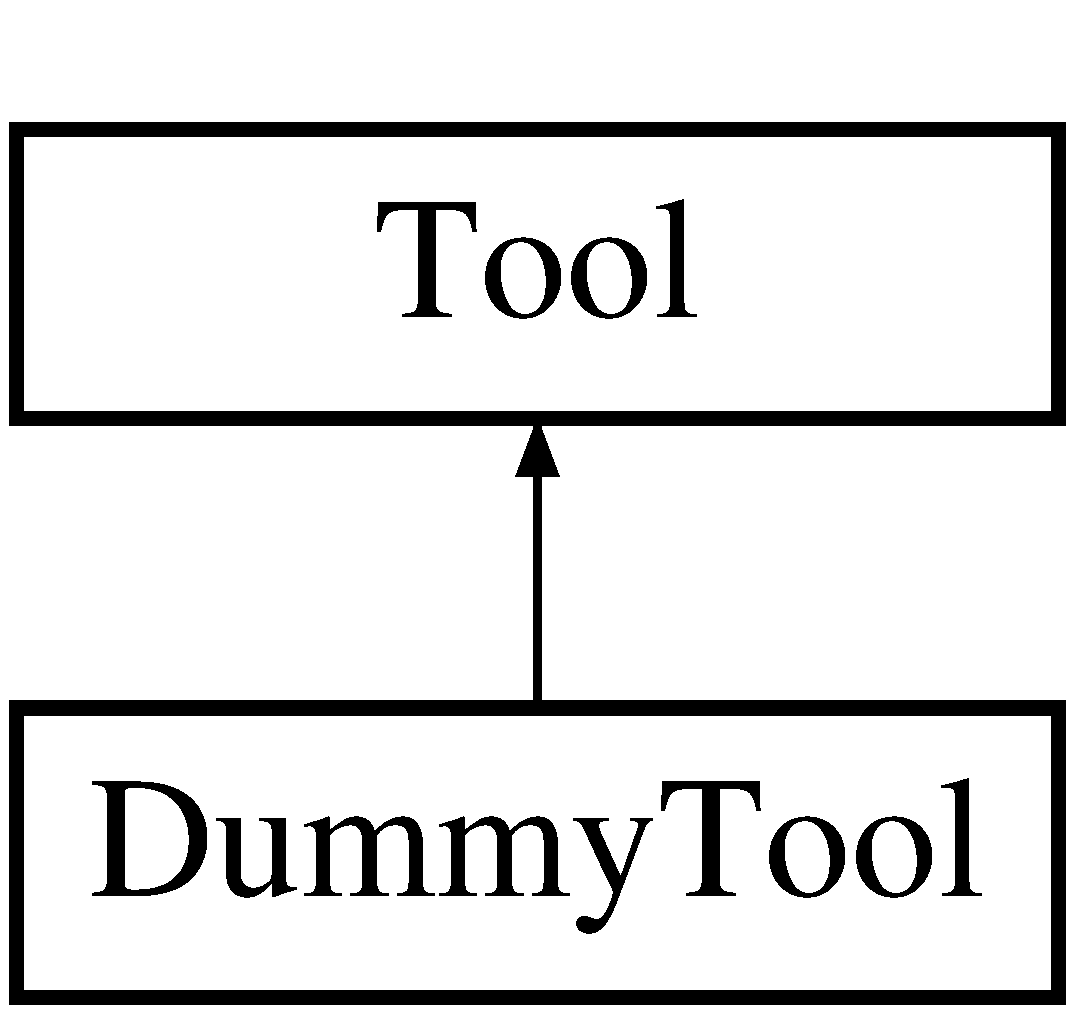
\includegraphics[height=2.000000cm]{classDummyTool}
\end{center}
\end{figure}
\subsection*{Public Member Functions}
\begin{DoxyCompactItemize}
\item 
\hypertarget{classDummyTool_a33914471b4de346168aa92b5febb6f9c}{\hyperlink{classDummyTool_a33914471b4de346168aa92b5febb6f9c}{Dummy\-Tool} ()}\label{classDummyTool_a33914471b4de346168aa92b5febb6f9c}

\begin{DoxyCompactList}\small\item\em Constructor. \end{DoxyCompactList}\item 
\hypertarget{classDummyTool_a0d9cd781681a06ee3cf0cd1e7bb770a8}{bool \hyperlink{classDummyTool_a0d9cd781681a06ee3cf0cd1e7bb770a8}{Initialise} (std\-::string configfile, \hyperlink{classDataModel}{Data\-Model} \&data)}\label{classDummyTool_a0d9cd781681a06ee3cf0cd1e7bb770a8}

\begin{DoxyCompactList}\small\item\em Assigns verbosity from config file and creates a log message. \end{DoxyCompactList}\item 
\hypertarget{classDummyTool_ac107b31f1785c1cc803e0e65be548047}{bool \hyperlink{classDummyTool_ac107b31f1785c1cc803e0e65be548047}{Execute} ()}\label{classDummyTool_ac107b31f1785c1cc803e0e65be548047}

\begin{DoxyCompactList}\small\item\em Creates a log message. \end{DoxyCompactList}\item 
\hypertarget{classDummyTool_aacb5d0b9906a27c2b4bba4aae9bc093a}{bool \hyperlink{classDummyTool_aacb5d0b9906a27c2b4bba4aae9bc093a}{Finalise} ()}\label{classDummyTool_aacb5d0b9906a27c2b4bba4aae9bc093a}

\begin{DoxyCompactList}\small\item\em Does nothing. \end{DoxyCompactList}\end{DoxyCompactItemize}


\subsection{Detailed Description}
This is a simple dummy Tool designed to show operation of a Tool. It also provides a default Tool for the Default Tool\-Chain.

\begin{DoxyParagraph}{Author\-:}
B.\-Richards 
\end{DoxyParagraph}
\begin{DoxyParagraph}{Date\-:}
2019/05/28 10\-:44\-:00 
\end{DoxyParagraph}
Contact\-: \href{mailto:b.richards@qmul.ac.uk}{\tt b.\-richards@qmul.\-ac.\-uk} 

The documentation for this class was generated from the following files\-:\begin{DoxyCompactItemize}
\item 
User\-Tools/\-Dummy\-Tool/Dummy\-Tool.\-h\item 
User\-Tools/\-Dummy\-Tool/Dummy\-Tool.\-cpp\end{DoxyCompactItemize}

\hypertarget{classEventDisplay}{
\section{EventDisplay Class Reference}
\label{classEventDisplay}\index{EventDisplay@{EventDisplay}}
}
\subsection*{Public Member Functions}
\begin{DoxyCompactItemize}
\item 
\hypertarget{classEventDisplay_afc7edf8f24c74b37c29355745b3cc4ad}{
bool {\bfseries Initialise} (std::string configfile, \hyperlink{classDataModel}{DataModel} \&data)}
\label{classEventDisplay_afc7edf8f24c74b37c29355745b3cc4ad}

\item 
\hypertarget{classEventDisplay_a3468ff690ccecd91c2b7ee84021d5e4b}{
bool {\bfseries Execute} ()}
\label{classEventDisplay_a3468ff690ccecd91c2b7ee84021d5e4b}

\item 
\hypertarget{classEventDisplay_a0fdfbdba7f66663ca61a2015c3f87a27}{
bool {\bfseries Finalise} ()}
\label{classEventDisplay_a0fdfbdba7f66663ca61a2015c3f87a27}

\item 
\hypertarget{classEventDisplay_a0badd7d4c163fd33246ef2fb5f3f5b11}{
void {\bfseries make\_\-gui} ()}
\label{classEventDisplay_a0badd7d4c163fd33246ef2fb5f3f5b11}

\item 
\hypertarget{classEventDisplay_acdb0b7db7007c50303e29321e8b178df}{
void {\bfseries draw\_\-event} ()}
\label{classEventDisplay_acdb0b7db7007c50303e29321e8b178df}

\item 
\hypertarget{classEventDisplay_a45064b5628a451ee019e2dc47fb80268}{
void {\bfseries draw\_\-event\_\-box} ()}
\label{classEventDisplay_a45064b5628a451ee019e2dc47fb80268}

\item 
\hypertarget{classEventDisplay_a7ffd0d9f6b41b5713655e11e8d79840c}{
void {\bfseries draw\_\-pmt\_\-legend} ()}
\label{classEventDisplay_a7ffd0d9f6b41b5713655e11e8d79840c}

\item 
\hypertarget{classEventDisplay_a1405448b0dafae76a5ff4bcbb1bc2fa4}{
void {\bfseries draw\_\-lappd\_\-legend} ()}
\label{classEventDisplay_a1405448b0dafae76a5ff4bcbb1bc2fa4}

\item 
\hypertarget{classEventDisplay_a69683e114fa3e1702ba154789672f492}{
void {\bfseries draw\_\-event\_\-PMTs} ()}
\label{classEventDisplay_a69683e114fa3e1702ba154789672f492}

\item 
\hypertarget{classEventDisplay_ae0d1b0fb901484e92518ec76061c5c9c}{
void {\bfseries draw\_\-event\_\-LAPPDs} ()}
\label{classEventDisplay_ae0d1b0fb901484e92518ec76061c5c9c}

\item 
\hypertarget{classEventDisplay_a8c3315cc4f055772b275e7a5c9593526}{
void {\bfseries draw\_\-event\_\-MRD} ()}
\label{classEventDisplay_a8c3315cc4f055772b275e7a5c9593526}

\item 
\hypertarget{classEventDisplay_a13ff76de80459d2b68e24dbd0b24416e}{
void {\bfseries draw\_\-true\_\-vertex} ()}
\label{classEventDisplay_a13ff76de80459d2b68e24dbd0b24416e}

\item 
\hypertarget{classEventDisplay_ad9e11e4c29bf6cd9c616e8a88c9450a5}{
void {\bfseries draw\_\-true\_\-ring} ()}
\label{classEventDisplay_ad9e11e4c29bf6cd9c616e8a88c9450a5}

\item 
\hypertarget{classEventDisplay_a0c142aae987bce6741becd4254993e4b}{
void {\bfseries delete\_\-canvas\_\-contents} ()}
\label{classEventDisplay_a0c142aae987bce6741becd4254993e4b}

\item 
\hypertarget{classEventDisplay_a8e03ad3c8e618e6781a8e085d4577083}{
void {\bfseries draw\_\-schematic\_\-detector} ()}
\label{classEventDisplay_a8e03ad3c8e618e6781a8e085d4577083}

\item 
\hypertarget{classEventDisplay_a8e0374381693a843b58d33ac4a3debd9}{
void {\bfseries set\_\-color\_\-palette} ()}
\label{classEventDisplay_a8e0374381693a843b58d33ac4a3debd9}

\item 
\hypertarget{classEventDisplay_a3e7298c6aab4ea268f51a6c805ccdc9a}{
void {\bfseries translate\_\-xy} (double vtxX, double vtxY, double vtxZ, double \&xWall, double \&yWall, int \&status\_\-hit, double \&phi\_\-calc)}
\label{classEventDisplay_a3e7298c6aab4ea268f51a6c805ccdc9a}

\item 
\hypertarget{classEventDisplay_a0a3b0b46289031922181d43a7db56271}{
void {\bfseries find\_\-projected\_\-xyz} (double vtxX, double vtxY, double vtxZ, double dirX, double dirY, double dirZ, double \&projected\_\-x, double \&projected\_\-y, double \&projected\_\-z)}
\label{classEventDisplay_a0a3b0b46289031922181d43a7db56271}

\end{DoxyCompactItemize}


The documentation for this class was generated from the following files:\begin{DoxyCompactItemize}
\item 
UserTools/EventDisplay/EventDisplay.h\item 
UserTools/EventDisplay/EventDisplay.cpp\end{DoxyCompactItemize}

\hypertarget{classEventSelector}{
\section{EventSelector Class Reference}
\label{classEventSelector}\index{EventSelector@{EventSelector}}
}
\subsection*{Public Types}
\begin{DoxyCompactItemize}
\item 
enum {\bfseries EventFlags} \{ \par
{\bfseries kFlagNone} =  0x00, 
{\bfseries kFlagMCFV} =  0x01, 
{\bfseries kFlagMCPMTVol} =  0x02, 
{\bfseries kFlagMCMRD} =  0x04, 
\par
{\bfseries kFlagMCPiK} =  0x08, 
{\bfseries kFlagRecoMRD} =  0x10, 
{\bfseries kFlagPromptTrig} =  0x20, 
{\bfseries kFlagNHit} =  0x40, 
\par
{\bfseries kFlagRecoFV} =  0x80, 
{\bfseries kFlagRecoPMTVol} =  0x100
 \}
\item 
\hypertarget{classEventSelector_ab9f5d192d2badda9754e2e91f430a012}{
typedef enum EventSelector::EventFlags {\bfseries EventFlags\_\-t}}
\label{classEventSelector_ab9f5d192d2badda9754e2e91f430a012}

\end{DoxyCompactItemize}
\subsection*{Public Member Functions}
\begin{DoxyCompactItemize}
\item 
bool \hyperlink{classEventSelector_a839f44332021b0345d0277f68ae612a8}{Initialise} (std::string configfile, \hyperlink{classDataModel}{DataModel} \&data)
\item 
bool \hyperlink{classEventSelector_a0edbb6c1b1a8c3fcd9453d3dd5796005}{Execute} ()
\item 
\hypertarget{classEventSelector_a73c813845d7cfce13f160e94b44b56c1}{
bool {\bfseries Finalise} ()}
\label{classEventSelector_a73c813845d7cfce13f160e94b44b56c1}

\end{DoxyCompactItemize}


\subsection{Member Function Documentation}
\hypertarget{classEventSelector_a0edbb6c1b1a8c3fcd9453d3dd5796005}{
\index{EventSelector@{EventSelector}!Execute@{Execute}}
\index{Execute@{Execute}!EventSelector@{EventSelector}}
\subsubsection[{Execute}]{\setlength{\rightskip}{0pt plus 5cm}bool EventSelector::Execute ()}}
\label{classEventSelector_a0edbb6c1b1a8c3fcd9453d3dd5796005}


$>$ Get digits from \char`\"{}RecoEvent\char`\"{}

$>$ Get reconstructed vertex \hypertarget{classEventSelector_a839f44332021b0345d0277f68ae612a8}{
\index{EventSelector@{EventSelector}!Initialise@{Initialise}}
\index{Initialise@{Initialise}!EventSelector@{EventSelector}}
\subsubsection[{Initialise}]{\setlength{\rightskip}{0pt plus 5cm}bool EventSelector::Initialise (std::string {\em configfile}, \/  {\bf DataModel} \& {\em data})}}
\label{classEventSelector_a839f44332021b0345d0277f68ae612a8}


Construct the other objects we'll be needing at event level, 

The documentation for this class was generated from the following files:\begin{DoxyCompactItemize}
\item 
UserTools/EventSelector/EventSelector.h\item 
UserTools/EventSelector/EventSelector.cpp\end{DoxyCompactItemize}

\hypertarget{classEventSelectorDoE}{
\section{EventSelectorDoE Class Reference}
\label{classEventSelectorDoE}\index{EventSelectorDoE@{EventSelectorDoE}}
}
\subsection*{Public Member Functions}
\begin{DoxyCompactItemize}
\item 
bool \hyperlink{classEventSelectorDoE_a9eef7438e552c60c6c11b3977d2f9210}{Initialise} (std::string configfile, \hyperlink{classDataModel}{DataModel} \&data)
\item 
\hypertarget{classEventSelectorDoE_afa76e234da6aef6333dca180b0a0e281}{
bool {\bfseries Execute} ()}
\label{classEventSelectorDoE_afa76e234da6aef6333dca180b0a0e281}

\item 
\hypertarget{classEventSelectorDoE_a2463b7db3877856bd0ce12b3e00dc8f9}{
bool {\bfseries Finalise} ()}
\label{classEventSelectorDoE_a2463b7db3877856bd0ce12b3e00dc8f9}

\end{DoxyCompactItemize}


\subsection{Member Function Documentation}
\hypertarget{classEventSelectorDoE_a9eef7438e552c60c6c11b3977d2f9210}{
\index{EventSelectorDoE@{EventSelectorDoE}!Initialise@{Initialise}}
\index{Initialise@{Initialise}!EventSelectorDoE@{EventSelectorDoE}}
\subsubsection[{Initialise}]{\setlength{\rightskip}{0pt plus 5cm}bool EventSelectorDoE::Initialise (std::string {\em configfile}, \/  {\bf DataModel} \& {\em data})}}
\label{classEventSelectorDoE_a9eef7438e552c60c6c11b3977d2f9210}


Construct the other objects we'll be setting at event level, 

The documentation for this class was generated from the following files:\begin{DoxyCompactItemize}
\item 
UserTools/EventSelectorDoE/EventSelectorDoE.h\item 
UserTools/EventSelectorDoE/EventSelectorDoE.cpp\end{DoxyCompactItemize}

\hypertarget{classExampleGenerateData}{
\section{ExampleGenerateData Class Reference}
\label{classExampleGenerateData}\index{ExampleGenerateData@{ExampleGenerateData}}
}
\subsection*{Public Member Functions}
\begin{DoxyCompactItemize}
\item 
\hypertarget{classExampleGenerateData_a34ef11ea9d2fe02c76c13227855538c7}{
bool {\bfseries Initialise} (std::string configfile, \hyperlink{classDataModel}{DataModel} \&data)}
\label{classExampleGenerateData_a34ef11ea9d2fe02c76c13227855538c7}

\item 
\hypertarget{classExampleGenerateData_a8ad50d91b736d2f11f48db3179ac7019}{
bool {\bfseries Execute} ()}
\label{classExampleGenerateData_a8ad50d91b736d2f11f48db3179ac7019}

\item 
\hypertarget{classExampleGenerateData_a7d27959b6641603076134866022f5ee9}{
bool {\bfseries Finalise} ()}
\label{classExampleGenerateData_a7d27959b6641603076134866022f5ee9}

\end{DoxyCompactItemize}


The documentation for this class was generated from the following files:\begin{DoxyCompactItemize}
\item 
UserTools/Examples/ExampleGenerateData.h\item 
UserTools/Examples/ExampleGenerateData.cpp\end{DoxyCompactItemize}

\hypertarget{classExampleLoadRoot}{
\section{ExampleLoadRoot Class Reference}
\label{classExampleLoadRoot}\index{ExampleLoadRoot@{ExampleLoadRoot}}
}
\subsection*{Public Member Functions}
\begin{DoxyCompactItemize}
\item 
\hypertarget{classExampleLoadRoot_a35f783852deea4191cf82812ccbd743c}{
bool {\bfseries Initialise} (std::string configfile, \hyperlink{classDataModel}{DataModel} \&data)}
\label{classExampleLoadRoot_a35f783852deea4191cf82812ccbd743c}

\item 
bool \hyperlink{classExampleLoadRoot_a463f4b53011e5fa862a3d39058305b83}{Execute} ()
\item 
\hypertarget{classExampleLoadRoot_aa919eb5fb4d16a7cf632b80a592970f2}{
bool {\bfseries Finalise} ()}
\label{classExampleLoadRoot_aa919eb5fb4d16a7cf632b80a592970f2}

\end{DoxyCompactItemize}


\subsection{Member Function Documentation}
\hypertarget{classExampleLoadRoot_a463f4b53011e5fa862a3d39058305b83}{
\index{ExampleLoadRoot@{ExampleLoadRoot}!Execute@{Execute}}
\index{Execute@{Execute}!ExampleLoadRoot@{ExampleLoadRoot}}
\subsubsection[{Execute}]{\setlength{\rightskip}{0pt plus 5cm}bool ExampleLoadRoot::Execute ()}}
\label{classExampleLoadRoot_a463f4b53011e5fa862a3d39058305b83}


saving to store for the sake of printing 

The documentation for this class was generated from the following files:\begin{DoxyCompactItemize}
\item 
UserTools/Examples/ExampleLoadRoot.h\item 
UserTools/Examples/ExampleLoadRoot.cpp\end{DoxyCompactItemize}

\hypertarget{classExampleloadStore}{\section{Exampleload\-Store Class Reference}
\label{classExampleloadStore}\index{Exampleload\-Store@{Exampleload\-Store}}
}
Inheritance diagram for Exampleload\-Store\-:\begin{figure}[H]
\begin{center}
\leavevmode
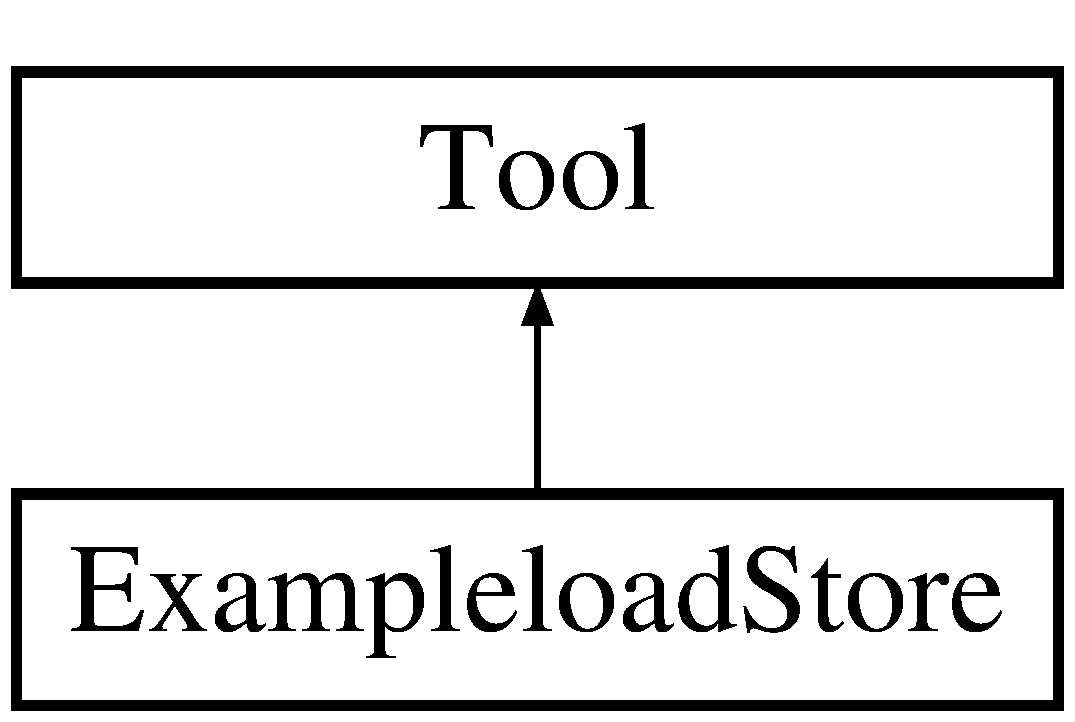
\includegraphics[height=2.000000cm]{classExampleloadStore}
\end{center}
\end{figure}
\subsection*{Public Member Functions}
\begin{DoxyCompactItemize}
\item 
\hypertarget{classExampleloadStore_aa36ea82e625367750cf90f47b68b4868}{bool {\bfseries Initialise} (std\-::string configfile, \hyperlink{classDataModel}{Data\-Model} \&data)}\label{classExampleloadStore_aa36ea82e625367750cf90f47b68b4868}

\item 
\hypertarget{classExampleloadStore_abb8ad989ae4890d9058989e9f4c1c5a7}{bool {\bfseries Execute} ()}\label{classExampleloadStore_abb8ad989ae4890d9058989e9f4c1c5a7}

\item 
\hypertarget{classExampleloadStore_a0170aae0ee1e46ea8e6132fb4874bb8d}{bool {\bfseries Finalise} ()}\label{classExampleloadStore_a0170aae0ee1e46ea8e6132fb4874bb8d}

\end{DoxyCompactItemize}


The documentation for this class was generated from the following files\-:\begin{DoxyCompactItemize}
\item 
User\-Tools/\-Examples/Exampleload\-Store.\-h\item 
User\-Tools/\-Examples/Exampleload\-Store.\-cpp\end{DoxyCompactItemize}

\hypertarget{classExampleOverTool}{
\section{ExampleOverTool Class Reference}
\label{classExampleOverTool}\index{ExampleOverTool@{ExampleOverTool}}
}
\subsection*{Public Member Functions}
\begin{DoxyCompactItemize}
\item 
\hypertarget{classExampleOverTool_ac7821b52bdffd736c9f4bb7265f2403c}{
bool {\bfseries Initialise} (std::string configfile, \hyperlink{classDataModel}{DataModel} \&data)}
\label{classExampleOverTool_ac7821b52bdffd736c9f4bb7265f2403c}

\item 
\hypertarget{classExampleOverTool_ae43f1902d5b79f6b474ba4b173ab0264}{
bool {\bfseries Execute} ()}
\label{classExampleOverTool_ae43f1902d5b79f6b474ba4b173ab0264}

\item 
\hypertarget{classExampleOverTool_aaf2c1cee9746ed6e94a9d58d8bc9fcae}{
bool {\bfseries Finalise} ()}
\label{classExampleOverTool_aaf2c1cee9746ed6e94a9d58d8bc9fcae}

\end{DoxyCompactItemize}


The documentation for this class was generated from the following files:\begin{DoxyCompactItemize}
\item 
UserTools/Examples/ExampleOverTool.h\item 
UserTools/Examples/ExampleOverTool.cpp\end{DoxyCompactItemize}

\hypertarget{classExamplePrintData}{\section{Example\-Print\-Data Class Reference}
\label{classExamplePrintData}\index{Example\-Print\-Data@{Example\-Print\-Data}}
}
Inheritance diagram for Example\-Print\-Data\-:\begin{figure}[H]
\begin{center}
\leavevmode
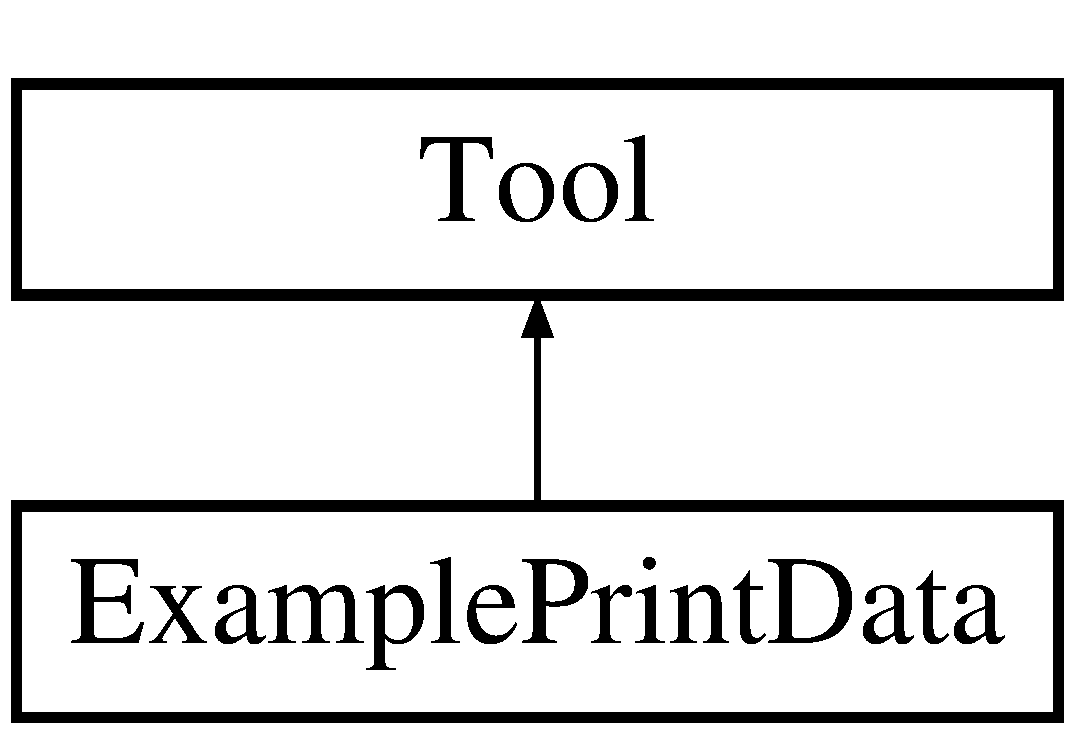
\includegraphics[height=2.000000cm]{classExamplePrintData}
\end{center}
\end{figure}
\subsection*{Public Member Functions}
\begin{DoxyCompactItemize}
\item 
\hypertarget{classExamplePrintData_a307dfd08e3e97a41630506b1796dc89f}{bool {\bfseries Initialise} (std\-::string configfile, \hyperlink{classDataModel}{Data\-Model} \&data)}\label{classExamplePrintData_a307dfd08e3e97a41630506b1796dc89f}

\item 
\hypertarget{classExamplePrintData_aa976e0555bc68a07f9525f556bb51352}{bool {\bfseries Execute} ()}\label{classExamplePrintData_aa976e0555bc68a07f9525f556bb51352}

\item 
\hypertarget{classExamplePrintData_a6b47fdbb41a982a082857c3fd94ac7a9}{bool {\bfseries Finalise} ()}\label{classExamplePrintData_a6b47fdbb41a982a082857c3fd94ac7a9}

\end{DoxyCompactItemize}


The documentation for this class was generated from the following files\-:\begin{DoxyCompactItemize}
\item 
User\-Tools/\-Examples/Example\-Print\-Data.\-h\item 
User\-Tools/\-Examples/Example\-Print\-Data.\-cpp\end{DoxyCompactItemize}

\hypertarget{classExampleRoot}{
\section{ExampleRoot Class Reference}
\label{classExampleRoot}\index{ExampleRoot@{ExampleRoot}}
}
\subsection*{Public Member Functions}
\begin{DoxyCompactItemize}
\item 
\hypertarget{classExampleRoot_a676a00459c76535ea0cc496333e0927f}{
{\bfseries ExampleRoot} (TTree $\ast$tree=0)}
\label{classExampleRoot_a676a00459c76535ea0cc496333e0927f}

\item 
\hypertarget{classExampleRoot_aa76fc5be93bb26800ef2d47b86db68ab}{
virtual Int\_\-t {\bfseries Cut} (Long64\_\-t entry)}
\label{classExampleRoot_aa76fc5be93bb26800ef2d47b86db68ab}

\item 
\hypertarget{classExampleRoot_aeaa244a73538e72d6d4431d6755e6aa9}{
virtual Int\_\-t {\bfseries GetEntry} (Long64\_\-t entry)}
\label{classExampleRoot_aeaa244a73538e72d6d4431d6755e6aa9}

\item 
\hypertarget{classExampleRoot_ad12d04e02467dc4541eaa95c112dfb65}{
virtual Long64\_\-t {\bfseries LoadTree} (Long64\_\-t entry)}
\label{classExampleRoot_ad12d04e02467dc4541eaa95c112dfb65}

\item 
\hypertarget{classExampleRoot_a6a24778d602dc1ecb97f8aeca9c2576c}{
virtual void {\bfseries Init} (TTree $\ast$tree)}
\label{classExampleRoot_a6a24778d602dc1ecb97f8aeca9c2576c}

\item 
\hypertarget{classExampleRoot_ac2cd7b771c6f1094df4278c2c81fa5d4}{
virtual void {\bfseries Loop} ()}
\label{classExampleRoot_ac2cd7b771c6f1094df4278c2c81fa5d4}

\item 
\hypertarget{classExampleRoot_ad2f3d94e1e75887a972eb220e55c6453}{
virtual Bool\_\-t {\bfseries Notify} ()}
\label{classExampleRoot_ad2f3d94e1e75887a972eb220e55c6453}

\item 
\hypertarget{classExampleRoot_ae352817f33d623e4a07ce448bc191533}{
virtual void {\bfseries Show} (Long64\_\-t entry=-\/1)}
\label{classExampleRoot_ae352817f33d623e4a07ce448bc191533}

\end{DoxyCompactItemize}
\subsection*{Public Attributes}
\begin{DoxyCompactItemize}
\item 
\hypertarget{classExampleRoot_a4717cece1b2513740bf12fe1b1f269cc}{
TTree $\ast$ {\bfseries fChain}}
\label{classExampleRoot_a4717cece1b2513740bf12fe1b1f269cc}

\item 
\hypertarget{classExampleRoot_aae45e22777e3dec49bc68fae4850cf63}{
Int\_\-t \hyperlink{classExampleRoot_aae45e22777e3dec49bc68fae4850cf63}{fCurrent}}
\label{classExampleRoot_aae45e22777e3dec49bc68fae4850cf63}

\begin{DoxyCompactList}\small\item\em pointer to the analyzed TTree or TChain \item\end{DoxyCompactList}\item 
\hypertarget{classExampleRoot_a184637f032bbd33058f288c631ad4b08}{
Int\_\-t \hyperlink{classExampleRoot_a184637f032bbd33058f288c631ad4b08}{a}}
\label{classExampleRoot_a184637f032bbd33058f288c631ad4b08}

\begin{DoxyCompactList}\small\item\em current Tree number in a TChain \item\end{DoxyCompactList}\item 
\hypertarget{classExampleRoot_a906499b01132e5c5e9c220ee2e7d75dd}{
Double\_\-t {\bfseries b}}
\label{classExampleRoot_a906499b01132e5c5e9c220ee2e7d75dd}

\item 
\hypertarget{classExampleRoot_aad0a4cee176922682ae2330e1613c978}{
std::string $\ast$ {\bfseries c}}
\label{classExampleRoot_aad0a4cee176922682ae2330e1613c978}

\item 
\hypertarget{classExampleRoot_adbbc71a9b714437196324a5144ba38d6}{
TBranch $\ast$ {\bfseries b\_\-a}}
\label{classExampleRoot_adbbc71a9b714437196324a5144ba38d6}

\item 
\hypertarget{classExampleRoot_a8c1be09581a81eb61c945ee01894f078}{
TBranch $\ast$ {\bfseries b\_\-b}}
\label{classExampleRoot_a8c1be09581a81eb61c945ee01894f078}

\item 
\hypertarget{classExampleRoot_ab3c9727dc708989f36140651ec6a898c}{
TBranch $\ast$ {\bfseries b\_\-c}}
\label{classExampleRoot_ab3c9727dc708989f36140651ec6a898c}

\end{DoxyCompactItemize}
\subsection*{Friends}
\begin{DoxyCompactItemize}
\item 
\hypertarget{classExampleRoot_ac98d07dd8f7b70e16ccb9a01abf56b9c}{
class {\bfseries boost::serialization::access}}
\label{classExampleRoot_ac98d07dd8f7b70e16ccb9a01abf56b9c}

\end{DoxyCompactItemize}


The documentation for this class was generated from the following files:\begin{DoxyCompactItemize}
\item 
DataModel/ExampleRoot.h\item 
DataModel/ExampleRoot.cpp\end{DoxyCompactItemize}

\hypertarget{classExampleSaveRoot}{\section{Example\-Save\-Root Class Reference}
\label{classExampleSaveRoot}\index{Example\-Save\-Root@{Example\-Save\-Root}}
}
Inheritance diagram for Example\-Save\-Root\-:\begin{figure}[H]
\begin{center}
\leavevmode
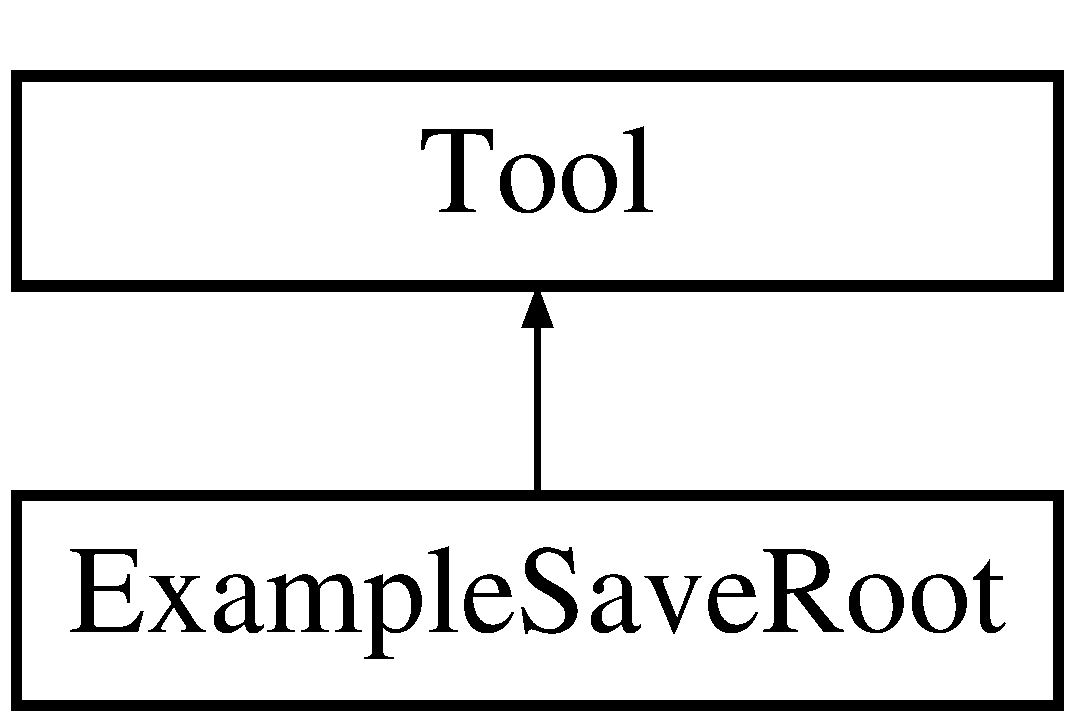
\includegraphics[height=2.000000cm]{classExampleSaveRoot}
\end{center}
\end{figure}
\subsection*{Public Member Functions}
\begin{DoxyCompactItemize}
\item 
\hypertarget{classExampleSaveRoot_a71c138625e281936faa6febe787a4f24}{bool {\bfseries Initialise} (std\-::string configfile, \hyperlink{classDataModel}{Data\-Model} \&data)}\label{classExampleSaveRoot_a71c138625e281936faa6febe787a4f24}

\item 
\hypertarget{classExampleSaveRoot_a5068a1d780f454298301ee6f26ac4357}{bool {\bfseries Execute} ()}\label{classExampleSaveRoot_a5068a1d780f454298301ee6f26ac4357}

\item 
\hypertarget{classExampleSaveRoot_a06f29407ff26756770b6e60eedae8ebf}{bool {\bfseries Finalise} ()}\label{classExampleSaveRoot_a06f29407ff26756770b6e60eedae8ebf}

\end{DoxyCompactItemize}


The documentation for this class was generated from the following files\-:\begin{DoxyCompactItemize}
\item 
User\-Tools/\-Examples/Example\-Save\-Root.\-h\item 
User\-Tools/\-Examples/Example\-Save\-Root.\-cpp\end{DoxyCompactItemize}

\hypertarget{classExampleSaveStore}{
\section{ExampleSaveStore Class Reference}
\label{classExampleSaveStore}\index{ExampleSaveStore@{ExampleSaveStore}}
}
\subsection*{Public Member Functions}
\begin{DoxyCompactItemize}
\item 
\hypertarget{classExampleSaveStore_a9c575471c5d024446e7b71b7340cc600}{
bool {\bfseries Initialise} (std::string configfile, \hyperlink{classDataModel}{DataModel} \&data)}
\label{classExampleSaveStore_a9c575471c5d024446e7b71b7340cc600}

\item 
\hypertarget{classExampleSaveStore_ab95ccff687c8114d6813a87c2bede948}{
bool {\bfseries Execute} ()}
\label{classExampleSaveStore_ab95ccff687c8114d6813a87c2bede948}

\item 
\hypertarget{classExampleSaveStore_aa28ea62a5f5bba4c04d271d502859e78}{
bool {\bfseries Finalise} ()}
\label{classExampleSaveStore_aa28ea62a5f5bba4c04d271d502859e78}

\end{DoxyCompactItemize}


The documentation for this class was generated from the following files:\begin{DoxyCompactItemize}
\item 
UserTools/Examples/ExampleSaveStore.h\item 
UserTools/Examples/ExampleSaveStore.cpp\end{DoxyCompactItemize}

\hypertarget{classFindMrdTracks}{\section{Find\-Mrd\-Tracks Class Reference}
\label{classFindMrdTracks}\index{Find\-Mrd\-Tracks@{Find\-Mrd\-Tracks}}
}
Inheritance diagram for Find\-Mrd\-Tracks\-:\begin{figure}[H]
\begin{center}
\leavevmode
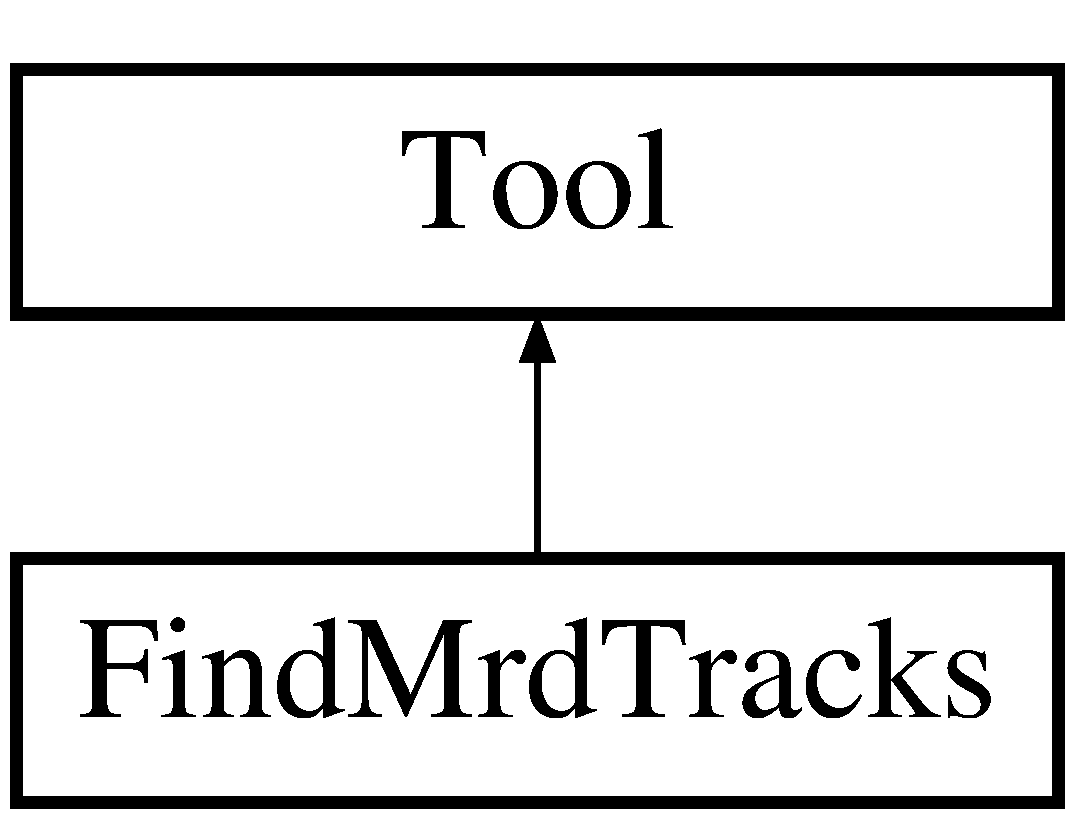
\includegraphics[height=2.000000cm]{classFindMrdTracks}
\end{center}
\end{figure}
\subsection*{Public Member Functions}
\begin{DoxyCompactItemize}
\item 
\hypertarget{classFindMrdTracks_a32cc40daea77e8fc6d4f64791922696e}{bool {\bfseries Initialise} (std\-::string configfile, \hyperlink{classDataModel}{Data\-Model} \&data)}\label{classFindMrdTracks_a32cc40daea77e8fc6d4f64791922696e}

\item 
\hypertarget{classFindMrdTracks_a24260dbeaee440f91c5aaad0af93886c}{bool {\bfseries Execute} ()}\label{classFindMrdTracks_a24260dbeaee440f91c5aaad0af93886c}

\item 
\hypertarget{classFindMrdTracks_a4c03c3790e73938bc9786981de31bab4}{bool {\bfseries Finalise} ()}\label{classFindMrdTracks_a4c03c3790e73938bc9786981de31bab4}

\item 
\hypertarget{classFindMrdTracks_acdbbb5dc3f26dcbc527d08483b2bcc9e}{void {\bfseries Start\-New\-File} ()}\label{classFindMrdTracks_acdbbb5dc3f26dcbc527d08483b2bcc9e}

\end{DoxyCompactItemize}


The documentation for this class was generated from the following files\-:\begin{DoxyCompactItemize}
\item 
User\-Tools/\-Find\-Mrd\-Tracks/Find\-Mrd\-Tracks.\-h\item 
User\-Tools/\-Find\-Mrd\-Tracks/Find\-Mrd\-Tracks.\-cpp\end{DoxyCompactItemize}

\hypertarget{classFindTrackLengthInWater}{\section{Find\-Track\-Length\-In\-Water Class Reference}
\label{classFindTrackLengthInWater}\index{Find\-Track\-Length\-In\-Water@{Find\-Track\-Length\-In\-Water}}
}
Inheritance diagram for Find\-Track\-Length\-In\-Water\-:\begin{figure}[H]
\begin{center}
\leavevmode
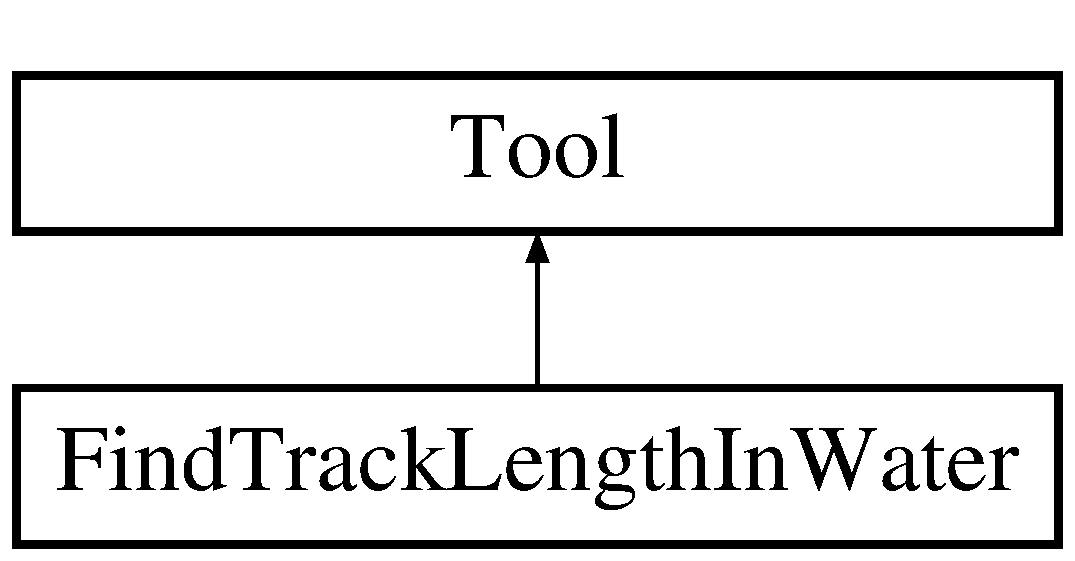
\includegraphics[height=2.000000cm]{classFindTrackLengthInWater}
\end{center}
\end{figure}
\subsection*{Public Member Functions}
\begin{DoxyCompactItemize}
\item 
\hypertarget{classFindTrackLengthInWater_a0f902c566760c2df0693cf00e99cc47e}{bool {\bfseries Initialise} (std\-::string configfile, \hyperlink{classDataModel}{Data\-Model} \&data)}\label{classFindTrackLengthInWater_a0f902c566760c2df0693cf00e99cc47e}

\item 
\hypertarget{classFindTrackLengthInWater_a27d29773eced4222f316ade698247d50}{bool {\bfseries Execute} ()}\label{classFindTrackLengthInWater_a27d29773eced4222f316ade698247d50}

\item 
\hypertarget{classFindTrackLengthInWater_a714975810be358a8b6c127a9b7992dc6}{double {\bfseries find\-\_\-lambda} (double xmu\-\_\-rec, double ymu\-\_\-rec, double zmu\-\_\-rec, double xrec\-Dir, double yrec\-Dir, double zrec\-Dir, double x\-\_\-pmtpos, double y\-\_\-pmtpos, double z\-\_\-pmtpos, double theta\-\_\-cher)}\label{classFindTrackLengthInWater_a714975810be358a8b6c127a9b7992dc6}

\item 
\hypertarget{classFindTrackLengthInWater_a1e9e6eaefc14833736544ebffb39eb1c}{bool {\bfseries Finalise} ()}\label{classFindTrackLengthInWater_a1e9e6eaefc14833736544ebffb39eb1c}

\end{DoxyCompactItemize}


The documentation for this class was generated from the following files\-:\begin{DoxyCompactItemize}
\item 
User\-Tools/\-Find\-Track\-Length\-In\-Water/Find\-Track\-Length\-In\-Water.\-h\item 
User\-Tools/\-Find\-Track\-Length\-In\-Water/Find\-Track\-Length\-In\-Water.\-cpp\end{DoxyCompactItemize}

\hypertarget{classFoMCalculator}{\section{Fo\-M\-Calculator Class Reference}
\label{classFoMCalculator}\index{Fo\-M\-Calculator@{Fo\-M\-Calculator}}
}
\subsection*{Public Member Functions}
\begin{DoxyCompactItemize}
\item 
\hypertarget{classFoMCalculator_a08e7a4cf1cbdeca75bde8d3c783eb543}{void {\bfseries Set\-Time\-Fit\-Weight} (double tweight)}\label{classFoMCalculator_a08e7a4cf1cbdeca75bde8d3c783eb543}

\item 
\hypertarget{classFoMCalculator_a7b70fa75561ef8047f4851e3572bea88}{void {\bfseries Set\-Cone\-Fit\-Weight} (double cweight)}\label{classFoMCalculator_a7b70fa75561ef8047f4851e3572bea88}

\item 
\hypertarget{classFoMCalculator_a410023f27226ff81d1c1f0c6d20d8121}{void {\bfseries Set\-Mean\-Time\-Calculator\-Type} (int type)}\label{classFoMCalculator_a410023f27226ff81d1c1f0c6d20d8121}

\item 
\hypertarget{classFoMCalculator_aa6a0ef5f03186fc3722f785104199abd}{void {\bfseries Load\-Vertex\-Geometry} (\hyperlink{classVertexGeometry}{Vertex\-Geometry} $\ast$vtxgeo)}\label{classFoMCalculator_aa6a0ef5f03186fc3722f785104199abd}

\item 
\hypertarget{classFoMCalculator_afc907bb278a95071410be7d0337253a1}{double {\bfseries Find\-Simple\-Time\-Properties} (double my\-Cone\-Edge)}\label{classFoMCalculator_afc907bb278a95071410be7d0337253a1}

\item 
\hypertarget{classFoMCalculator_ad62643573ab780bf3329d0c48f615c7a}{void {\bfseries Time\-Properties\-Ln\-L} (double vtx\-Time, double \&vtx\-Fom)}\label{classFoMCalculator_ad62643573ab780bf3329d0c48f615c7a}

\item 
\hypertarget{classFoMCalculator_a8697cdce3d92b4c8afb843b4e20ae0cd}{void {\bfseries Cone\-Properties\-Fo\-M} (double cone\-Edge, double \&chi2)}\label{classFoMCalculator_a8697cdce3d92b4c8afb843b4e20ae0cd}

\item 
\hypertarget{classFoMCalculator_a14d1020216db6fc5149b7918e8138b0b}{void {\bfseries Point\-Position\-Chi2} (double vtx\-X, double vtx\-Y, double vtx\-Z, double vtx\-Time, double \&fom)}\label{classFoMCalculator_a14d1020216db6fc5149b7918e8138b0b}

\item 
\hypertarget{classFoMCalculator_a275afaff36e1d93e732811382c433566}{void {\bfseries Point\-Direction\-Chi2} (double vtx\-X, double vtx\-Y, double vtx\-Z, double dir\-X, double dir\-Y, double dir\-Z, double cone\-Angle, double \&fom)}\label{classFoMCalculator_a275afaff36e1d93e732811382c433566}

\item 
\hypertarget{classFoMCalculator_a6fc036ee8918755886ffa842e5c5d781}{void {\bfseries Point\-Vertex\-Chi2} (double vtx\-X, double vtx\-Y, double vtx\-Z, double dir\-X, double dir\-Y, double dir\-Z, double cone\-Angle, double vtx\-Time, double \&fom)}\label{classFoMCalculator_a6fc036ee8918755886ffa842e5c5d781}

\item 
\hypertarget{classFoMCalculator_a419589ed8639a623dec06684e57d0db5}{void {\bfseries Extended\-Vertex\-Chi2} (double vtx\-X, double vtx\-Y, double vtx\-Z, double dir\-X, double dir\-Y, double dir\-Z, double cone\-Angle, double vtx\-Time, double \&fom)}\label{classFoMCalculator_a419589ed8639a623dec06684e57d0db5}

\end{DoxyCompactItemize}
\subsection*{Public Attributes}
\begin{DoxyCompactItemize}
\item 
\hypertarget{classFoMCalculator_a3a7bca0306b8b1570e639b863ed7e92e}{double {\bfseries f\-Base\-F\-O\-M}}\label{classFoMCalculator_a3a7bca0306b8b1570e639b863ed7e92e}

\item 
\hypertarget{classFoMCalculator_ae9c9449bfa160d8c5d241ab3b729a10b}{double {\bfseries f\-Time\-Fit\-Weight}}\label{classFoMCalculator_ae9c9449bfa160d8c5d241ab3b729a10b}

\item 
\hypertarget{classFoMCalculator_a74a5ae95c46e77c0d70f346ddf5ac7b4}{double {\bfseries f\-Cone\-Fit\-Weight}}\label{classFoMCalculator_a74a5ae95c46e77c0d70f346ddf5ac7b4}

\item 
\hypertarget{classFoMCalculator_ae80b01958ac5f9513b46406ac46ac486}{int {\bfseries f\-Mean\-Time\-Calculator\-Type}}\label{classFoMCalculator_ae80b01958ac5f9513b46406ac46ac486}

\item 
\hypertarget{classFoMCalculator_a8962e8746e1e5a857c73c1d3c2b350ee}{\hyperlink{classVertexGeometry}{Vertex\-Geometry} $\ast$ {\bfseries f\-Vtx\-Geo}}\label{classFoMCalculator_a8962e8746e1e5a857c73c1d3c2b350ee}

\end{DoxyCompactItemize}


The documentation for this class was generated from the following files\-:\begin{DoxyCompactItemize}
\item 
Data\-Model/Fo\-M\-Calculator.\-h\item 
Data\-Model/Fo\-M\-Calculator.\-cpp\end{DoxyCompactItemize}

\hypertarget{classGenerateHits}{\section{Generate\-Hits Class Reference}
\label{classGenerateHits}\index{Generate\-Hits@{Generate\-Hits}}
}
Inheritance diagram for Generate\-Hits\-:\begin{figure}[H]
\begin{center}
\leavevmode
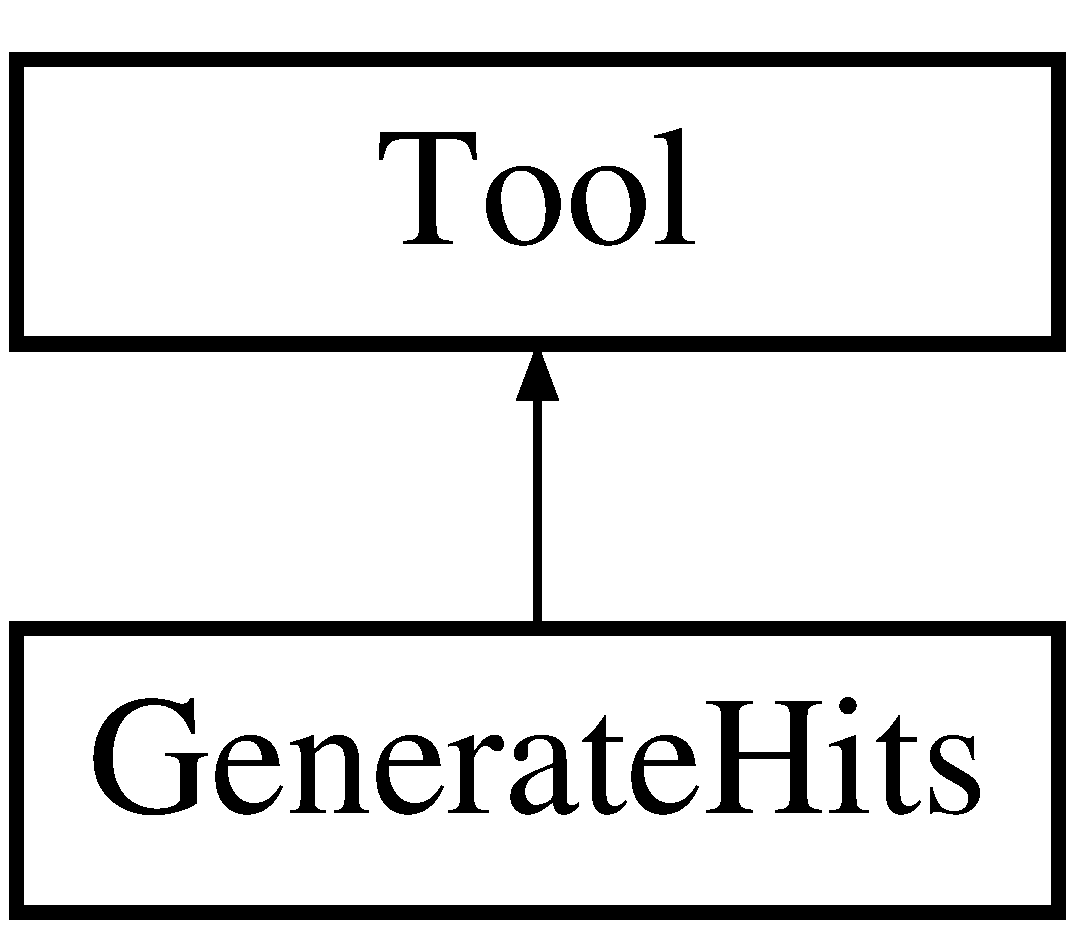
\includegraphics[height=2.000000cm]{classGenerateHits}
\end{center}
\end{figure}
\subsection*{Public Member Functions}
\begin{DoxyCompactItemize}
\item 
\hypertarget{classGenerateHits_a11c98b7819edf56f56d1981b72ed9e24}{bool {\bfseries Initialise} (std\-::string configfile, \hyperlink{classDataModel}{Data\-Model} \&data)}\label{classGenerateHits_a11c98b7819edf56f56d1981b72ed9e24}

\item 
\hypertarget{classGenerateHits_a3bf8e799c8fd096b2b3e802693fc043d}{bool {\bfseries Execute} ()}\label{classGenerateHits_a3bf8e799c8fd096b2b3e802693fc043d}

\item 
\hypertarget{classGenerateHits_a2c84756b951a63d38a6601a61334895d}{bool {\bfseries Finalise} ()}\label{classGenerateHits_a2c84756b951a63d38a6601a61334895d}

\end{DoxyCompactItemize}


The documentation for this class was generated from the following files\-:\begin{DoxyCompactItemize}
\item 
User\-Tools/\-Generate\-Hits/Generate\-Hits.\-h\item 
User\-Tools/\-Generate\-Hits/Generate\-Hits.\-cpp\end{DoxyCompactItemize}

\hypertarget{classGeometry}{\section{Geometry Class Reference}
\label{classGeometry}\index{Geometry@{Geometry}}
}
Inheritance diagram for Geometry\-:\begin{figure}[H]
\begin{center}
\leavevmode
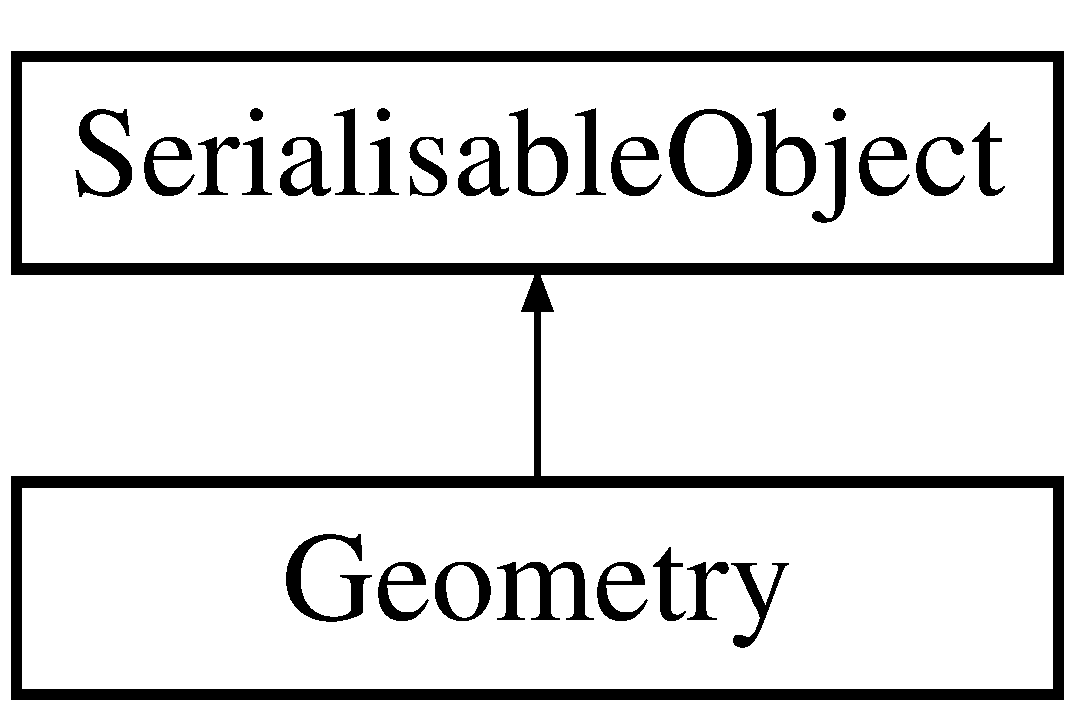
\includegraphics[height=2.000000cm]{classGeometry}
\end{center}
\end{figure}
\subsection*{Public Member Functions}
\begin{DoxyCompactItemize}
\item 
\hypertarget{classGeometry_ab5170692a6cbe471976e851f79e9319a}{Real\-Detectors {\bfseries reserve} (10)}\label{classGeometry_ab5170692a6cbe471976e851f79e9319a}

\item 
\hypertarget{classGeometry_a6f68b0647ccbaf76ba714730451dc3cf}{{\bfseries Geometry} (double ver, \hyperlink{classPosition}{Position} tankc, double tankr, double tankhh, double pmtencr, double pmtenchh, double mrdw, double mrdh, double mrdd, double mrds, int ntankpmts, int nmrdpmts, int nvetopmts, int nlappds, geostatus statin, std\-::vector$<$ std\-::map$<$ unsigned long, \hyperlink{classDetector}{Detector} $>$ $\ast$ $>$dets=std\-::vector$<$ std\-::map$<$ unsigned long, \hyperlink{classDetector}{Detector} $>$ $\ast$ $>$\{\})}\label{classGeometry_a6f68b0647ccbaf76ba714730451dc3cf}

\item 
\hypertarget{classGeometry_afbfabb07e8f8cad1496e2b69db8addb8}{std\-::vector$<$ std\-::map\\*
$<$ unsigned long, \hyperlink{classDetector}{Detector} $>$ $\ast$ $>$ $\ast$ {\bfseries Get\-Detectors} ()}\label{classGeometry_afbfabb07e8f8cad1496e2b69db8addb8}

\item 
\hypertarget{classGeometry_a94c52a826664f141dd3246fa1478a475}{double {\bfseries Get\-Version} ()}\label{classGeometry_a94c52a826664f141dd3246fa1478a475}

\item 
\hypertarget{classGeometry_a21835bb3d23fd54895350c84471dfb02}{geostatus {\bfseries Get\-Status} ()}\label{classGeometry_a21835bb3d23fd54895350c84471dfb02}

\item 
\hypertarget{classGeometry_a804b7ce9d8f1abe1ce5fffe9da65af51}{\hyperlink{classPosition}{Position} {\bfseries Get\-Tank\-Centre} ()}\label{classGeometry_a804b7ce9d8f1abe1ce5fffe9da65af51}

\item 
\hypertarget{classGeometry_abc3f55a2c64ec9f83a0ea7e82724fe49}{double {\bfseries Get\-Tank\-Radius} ()}\label{classGeometry_abc3f55a2c64ec9f83a0ea7e82724fe49}

\item 
\hypertarget{classGeometry_acc0459993448786f92dbdad8c4652176}{double {\bfseries Get\-Tank\-Halfheight} ()}\label{classGeometry_acc0459993448786f92dbdad8c4652176}

\item 
\hypertarget{classGeometry_abd765c4d73ceba92e39d007b6c3362bd}{double {\bfseries Get\-P\-M\-T\-Enclosed\-Radius} ()}\label{classGeometry_abd765c4d73ceba92e39d007b6c3362bd}

\item 
\hypertarget{classGeometry_a42b716a80c24a5278099e7ae8515dd69}{double {\bfseries Get\-P\-M\-T\-Enclosed\-Halfheight} ()}\label{classGeometry_a42b716a80c24a5278099e7ae8515dd69}

\item 
\hypertarget{classGeometry_ad33910b8b84b8956ecbfa4954a7ccfcc}{double {\bfseries Get\-Fiducial\-Cut\-Radius} ()}\label{classGeometry_ad33910b8b84b8956ecbfa4954a7ccfcc}

\item 
\hypertarget{classGeometry_a849d59159bc9afef2fb5a5de1b8f920d}{double {\bfseries Get\-Fiducial\-Cut\-Y} ()}\label{classGeometry_a849d59159bc9afef2fb5a5de1b8f920d}

\item 
\hypertarget{classGeometry_a858a7eafaa3c0629e596d1abf3e9346b}{double {\bfseries Get\-Fiducial\-Cut\-Z} ()}\label{classGeometry_a858a7eafaa3c0629e596d1abf3e9346b}

\item 
\hypertarget{classGeometry_a7dc78bc77bd7e01df60c513e3c1f3a8d}{double {\bfseries Get\-Mrd\-Width} ()}\label{classGeometry_a7dc78bc77bd7e01df60c513e3c1f3a8d}

\item 
\hypertarget{classGeometry_ad89709f6efbf3119c90da8e7631e1024}{double {\bfseries Get\-Mrd\-Height} ()}\label{classGeometry_ad89709f6efbf3119c90da8e7631e1024}

\item 
\hypertarget{classGeometry_a867b5607dbd4d3baeed4f03317026af5}{double {\bfseries Get\-Mrd\-Depth} ()}\label{classGeometry_a867b5607dbd4d3baeed4f03317026af5}

\item 
\hypertarget{classGeometry_a43cefba896c4f17a1607b658ae81c47d}{double {\bfseries Get\-Mrd\-Start} ()}\label{classGeometry_a43cefba896c4f17a1607b658ae81c47d}

\item 
\hypertarget{classGeometry_a61a5beb5c95207de729dddb94670ad55}{double {\bfseries Get\-Mrd\-End} ()}\label{classGeometry_a61a5beb5c95207de729dddb94670ad55}

\item 
\hypertarget{classGeometry_afdc0b24374cc8906be35ea93d1c99520}{void {\bfseries Set\-Version} (double Version\-In)}\label{classGeometry_afdc0b24374cc8906be35ea93d1c99520}

\item 
\hypertarget{classGeometry_a2ecdbc2a94b827fa0c372da34138d77f}{void {\bfseries Set\-Status} (geostatus Status\-In)}\label{classGeometry_a2ecdbc2a94b827fa0c372da34138d77f}

\item 
\hypertarget{classGeometry_ac333cb9fd34843161769b5eaf084219f}{void {\bfseries Set\-Tank\-Centre} (\hyperlink{classPosition}{Position} tank\-\_\-centrein)}\label{classGeometry_ac333cb9fd34843161769b5eaf084219f}

\item 
\hypertarget{classGeometry_a0f2d050fa42af21e6e0b4914974b45f5}{void {\bfseries Set\-Tank\-Radius} (double tank\-\_\-radius\-In)}\label{classGeometry_a0f2d050fa42af21e6e0b4914974b45f5}

\item 
\hypertarget{classGeometry_aae1817255945967705d105665b2fb248}{void {\bfseries Set\-Tank\-Halfheight} (double tank\-\_\-halfheight\-In)}\label{classGeometry_aae1817255945967705d105665b2fb248}

\item 
\hypertarget{classGeometry_a220d86cc649f42a16d33c73c1fc9e70e}{void {\bfseries Set\-P\-M\-T\-Enclosed\-Radius} (double pmt\-\_\-enclosed\-\_\-radius\-In)}\label{classGeometry_a220d86cc649f42a16d33c73c1fc9e70e}

\item 
\hypertarget{classGeometry_aca093a4eaad96fa51b4bac6fbe5fc5b6}{void {\bfseries Set\-P\-M\-T\-Enclosed\-Halfheight} (double pmt\-\_\-enclosed\-\_\-halfheight\-In)}\label{classGeometry_aca093a4eaad96fa51b4bac6fbe5fc5b6}

\item 
\hypertarget{classGeometry_a88cbe634b7185c5230f925a182599dd1}{void {\bfseries Set\-Fiducial\-Cut\-Radius} (double fidcutradiusin)}\label{classGeometry_a88cbe634b7185c5230f925a182599dd1}

\item 
\hypertarget{classGeometry_acddde32956d96095d3deb2d00c90a3ee}{void {\bfseries Set\-Fiducial\-Cut\-Z} (double fidcutzin)}\label{classGeometry_acddde32956d96095d3deb2d00c90a3ee}

\item 
\hypertarget{classGeometry_a808167f759b49e7958abe1598d6b6294}{void {\bfseries Set\-Fiducial\-Cut\-Y} (double fidcutyin)}\label{classGeometry_a808167f759b49e7958abe1598d6b6294}

\item 
\hypertarget{classGeometry_a120524e0dcd97fdea137b49b976a5183}{void {\bfseries Set\-Mrd\-Width} (double mrd\-\_\-width\-In)}\label{classGeometry_a120524e0dcd97fdea137b49b976a5183}

\item 
\hypertarget{classGeometry_a42377661ec147b299c500e9aa49aaf54}{void {\bfseries Set\-Mrd\-Height} (double mrd\-\_\-height\-In)}\label{classGeometry_a42377661ec147b299c500e9aa49aaf54}

\item 
\hypertarget{classGeometry_a44da646292c6c7e83709e8aa47236844}{void {\bfseries Set\-Mrd\-Depth} (double mrd\-\_\-depth\-In)}\label{classGeometry_a44da646292c6c7e83709e8aa47236844}

\item 
\hypertarget{classGeometry_a100d585e24c6c52794741e280d4dd4c6}{void {\bfseries Set\-Mrd\-Start} (double mrd\-\_\-start\-In)}\label{classGeometry_a100d585e24c6c52794741e280d4dd4c6}

\item 
\hypertarget{classGeometry_a2543a2a6d20336cc25a26fba69245955}{void {\bfseries Set\-Detectors} (std\-::vector$<$ std\-::map$<$ unsigned long, \hyperlink{classDetector}{Detector} $>$ $\ast$ $>$Detectors\-In)}\label{classGeometry_a2543a2a6d20336cc25a26fba69245955}

\item 
\hypertarget{classGeometry_ac5f3c966b7862b10af20fb83c9c45082}{unsigned long {\bfseries Consume\-Next\-Free\-Channel\-Key} ()}\label{classGeometry_ac5f3c966b7862b10af20fb83c9c45082}

\item 
\hypertarget{classGeometry_aea3868f7e8a725f672a2e488fe95eb5f}{unsigned long {\bfseries Consume\-Next\-Free\-Detector\-Key} ()}\label{classGeometry_aea3868f7e8a725f672a2e488fe95eb5f}

\item 
\hypertarget{classGeometry_aedc8d0b00db707eb63177b3fbc55e7f7}{bool {\bfseries Add\-Detector} (\hyperlink{classDetector}{Detector} detin)}\label{classGeometry_aedc8d0b00db707eb63177b3fbc55e7f7}

\item 
\hypertarget{classGeometry_a9c164587d17b71fb8cbcfa0535dca18f}{int {\bfseries Get\-Num\-Detectors} ()}\label{classGeometry_a9c164587d17b71fb8cbcfa0535dca18f}

\item 
\hypertarget{classGeometry_a3b4131297b0329603c7700e7eed9cf0b}{\hyperlink{classDetector}{Detector} $\ast$ {\bfseries Get\-Detector} (unsigned long Detector\-Key)}\label{classGeometry_a3b4131297b0329603c7700e7eed9cf0b}

\item 
\hypertarget{classGeometry_a6091d6b92a17207fdda50a03cc64b381}{\hyperlink{classDetector}{Detector} $\ast$ {\bfseries Channel\-To\-Detector} (unsigned long \hyperlink{classChannelKey}{Channel\-Key})}\label{classGeometry_a6091d6b92a17207fdda50a03cc64b381}

\item 
\hypertarget{classGeometry_a68873d502689bb73337c3f8d6e0ef3bf}{\hyperlink{classChannel}{Channel} $\ast$ {\bfseries Get\-Channel} (unsigned long \hyperlink{classChannelKey}{Channel\-Key})}\label{classGeometry_a68873d502689bb73337c3f8d6e0ef3bf}

\item 
\hypertarget{classGeometry_a60e84520417769401492de9e182636fc}{void {\bfseries Init\-Channel\-Map} ()}\label{classGeometry_a60e84520417769401492de9e182636fc}

\item 
\hypertarget{classGeometry_a4354935089665d2856b9a9a5bb1f181a}{int {\bfseries Get\-Num\-Detectors\-In\-Set} (std\-::string Set\-Name)}\label{classGeometry_a4354935089665d2856b9a9a5bb1f181a}

\item 
\hypertarget{classGeometry_aca1dd1c2919c14b2d8bdf40db23c5ba9}{bool {\bfseries Get\-Tank\-Contained} (\hyperlink{classParticle}{Particle} part, int startstop=0)}\label{classGeometry_aca1dd1c2919c14b2d8bdf40db23c5ba9}

\item 
\hypertarget{classGeometry_a2c68539bcaaf45158dbcdc50c3f65ca6}{bool {\bfseries Get\-Tank\-Contained} (\hyperlink{classPosition}{Position} a\-Vertex)}\label{classGeometry_a2c68539bcaaf45158dbcdc50c3f65ca6}

\item 
\hypertarget{classGeometry_af4c8b8f5df92cf905e0ea7098ceb52ed}{bool {\bfseries Get\-Mrd\-Contained} (\hyperlink{classParticle}{Particle} part, int startstop=0)}\label{classGeometry_af4c8b8f5df92cf905e0ea7098ceb52ed}

\item 
\hypertarget{classGeometry_a9da73da227027f3592e9ef10cb06033f}{bool {\bfseries Get\-Mrd\-Contained} (\hyperlink{classPosition}{Position} a\-Vertex)}\label{classGeometry_a9da73da227027f3592e9ef10cb06033f}

\item 
\hypertarget{classGeometry_a5ddd7d7d95f76d8d711c9727824020ca}{bool {\bfseries Print} ()}\label{classGeometry_a5ddd7d7d95f76d8d711c9727824020ca}

\item 
\hypertarget{classGeometry_acf8cf2161abe0c73a4f285f66277f2cd}{bool {\bfseries Print\-Status} (geostatus status)}\label{classGeometry_acf8cf2161abe0c73a4f285f66277f2cd}

\item 
\hypertarget{classGeometry_a12b34f2e75cdee8441008d9de7e2eb1b}{void {\bfseries Print\-Channels} ()}\label{classGeometry_a12b34f2e75cdee8441008d9de7e2eb1b}

\item 
\hypertarget{classGeometry_af1ef26f91bb256a2a7d52c37f502acc7}{\hyperlink{classPosition}{Position} {\bfseries Global\-To\-Tank\-Centered} (\hyperlink{classPosition}{Position} posin)}\label{classGeometry_af1ef26f91bb256a2a7d52c37f502acc7}

\item 
\hypertarget{classGeometry_a89335cdbf640744d7e4362d8495b6859}{void {\bfseries Cartesian\-To\-Polar} (\hyperlink{classPosition}{Position} posin, double \&R, double \&Phi, double \&Theta, bool tankcentered=false)}\label{classGeometry_a89335cdbf640744d7e4362d8495b6859}

\end{DoxyCompactItemize}
\subsection*{Friends}
\begin{DoxyCompactItemize}
\item 
\hypertarget{classGeometry_ac98d07dd8f7b70e16ccb9a01abf56b9c}{class {\bfseries boost\-::serialization\-::access}}\label{classGeometry_ac98d07dd8f7b70e16ccb9a01abf56b9c}

\end{DoxyCompactItemize}


The documentation for this class was generated from the following files\-:\begin{DoxyCompactItemize}
\item 
Data\-Model/Geometry.\-h\item 
Data\-Model/Geometry.\-cpp\end{DoxyCompactItemize}

\hypertarget{classHeftyInfo}{\section{Hefty\-Info Class Reference}
\label{classHeftyInfo}\index{Hefty\-Info@{Hefty\-Info}}
}
Inheritance diagram for Hefty\-Info\-:\begin{figure}[H]
\begin{center}
\leavevmode
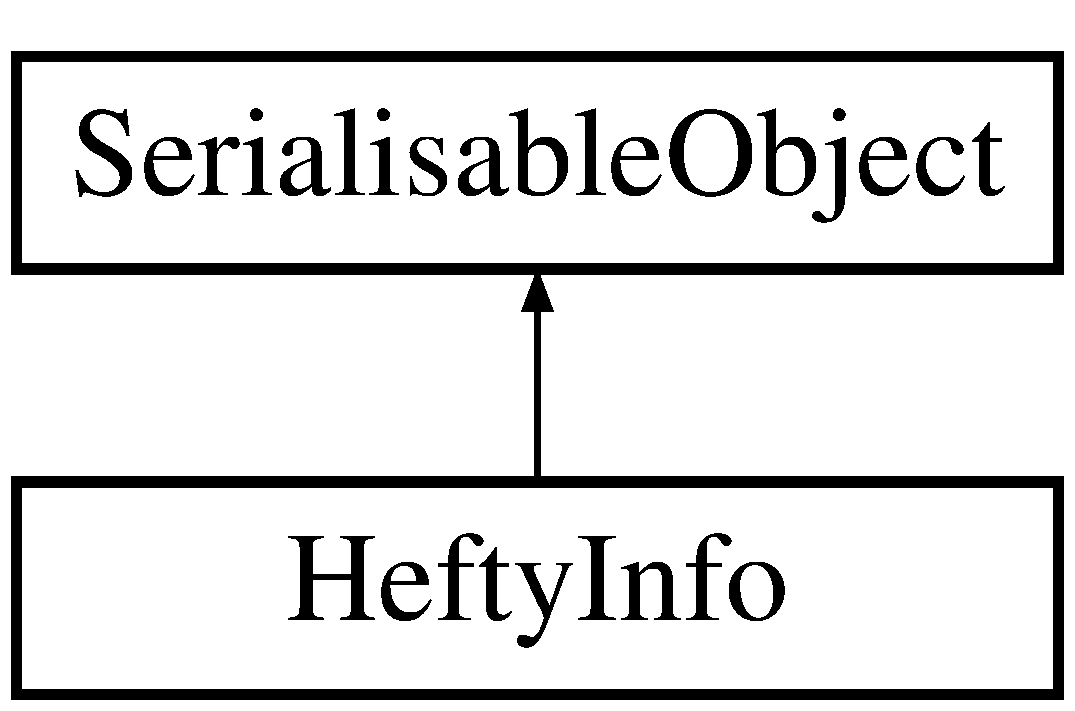
\includegraphics[height=2.000000cm]{classHeftyInfo}
\end{center}
\end{figure}
\subsection*{Public Member Functions}
\begin{DoxyCompactItemize}
\item 
\hypertarget{classHeftyInfo_af721faddd429a02ea7651108185ec478}{{\bfseries Hefty\-Info} (int sequence\-\_\-id, const std\-::vector$<$ unsigned long long $>$ \&time, const std\-::vector$<$ int $>$ \&label, const std\-::vector$<$ long long $>$ \&t\-\_\-since\-\_\-beam, const std\-::vector$<$ int $>$ \&more)}\label{classHeftyInfo_af721faddd429a02ea7651108185ec478}

\item 
\hypertarget{classHeftyInfo_a1e9b9d3197a8df5bff0432f1f814109b}{size\-\_\-t {\bfseries num\-\_\-minibuffers} () const }\label{classHeftyInfo_a1e9b9d3197a8df5bff0432f1f814109b}

\item 
\hypertarget{classHeftyInfo_ab9b5565e7b54b73eb83fd72c3e10a349}{int {\bfseries sequence\-\_\-id} () const }\label{classHeftyInfo_ab9b5565e7b54b73eb83fd72c3e10a349}

\item 
\hypertarget{classHeftyInfo_a9da6b668891f3a104f5fe6b5026e0969}{unsigned long long {\bfseries time} (size\-\_\-t mb) const }\label{classHeftyInfo_a9da6b668891f3a104f5fe6b5026e0969}

\item 
\hypertarget{classHeftyInfo_a2455de20fa2e072b68f58f37307c1989}{int {\bfseries label} (size\-\_\-t mb) const }\label{classHeftyInfo_a2455de20fa2e072b68f58f37307c1989}

\item 
\hypertarget{classHeftyInfo_a6880deb111e4b3f3d1d0bf0be8e4290e}{long long {\bfseries t\-\_\-since\-\_\-beam} (size\-\_\-t mb) const }\label{classHeftyInfo_a6880deb111e4b3f3d1d0bf0be8e4290e}

\item 
\hypertarget{classHeftyInfo_abb3cfed8ce0e9d03024d62a5687746cc}{bool {\bfseries more} () const }\label{classHeftyInfo_abb3cfed8ce0e9d03024d62a5687746cc}

\item 
\hypertarget{classHeftyInfo_a9f6297619ba660d09a294ad599d3273e}{std\-::vector$<$ unsigned long long $>$ {\bfseries all\-\_\-times} () const }\label{classHeftyInfo_a9f6297619ba660d09a294ad599d3273e}

\item 
\hypertarget{classHeftyInfo_a4184a22ba444cbfcc94b95bc5b0df49b}{virtual bool {\bfseries Print} () override}\label{classHeftyInfo_a4184a22ba444cbfcc94b95bc5b0df49b}

\end{DoxyCompactItemize}
\subsection*{Protected Member Functions}
\begin{DoxyCompactItemize}
\item 
\hypertarget{classHeftyInfo_a767538957878f8f708677d353c7a41db}{{\footnotesize template$<$class Archive $>$ }\\void {\bfseries serialize} (Archive \&ar, const unsigned int version)}\label{classHeftyInfo_a767538957878f8f708677d353c7a41db}

\end{DoxyCompactItemize}
\subsection*{Protected Attributes}
\begin{DoxyCompactItemize}
\item 
\hypertarget{classHeftyInfo_a0dab6f58a2c3719e087bc18b6e32e528}{int {\bfseries sequence\-\_\-id\-\_\-}}\label{classHeftyInfo_a0dab6f58a2c3719e087bc18b6e32e528}

\item 
\hypertarget{classHeftyInfo_a49dcdefaf94072a936aaba0f4d335b7b}{std\-::vector$<$ unsigned long long $>$ {\bfseries time\-\_\-}}\label{classHeftyInfo_a49dcdefaf94072a936aaba0f4d335b7b}

\item 
\hypertarget{classHeftyInfo_a8c18908b972555f6da8137ff67124eaf}{std\-::vector$<$ int $>$ {\bfseries label\-\_\-}}\label{classHeftyInfo_a8c18908b972555f6da8137ff67124eaf}

\item 
\hypertarget{classHeftyInfo_a68c89d555a59e08992862804591d4876}{std\-::vector$<$ long long $>$ {\bfseries t\-\_\-since\-\_\-beam\-\_\-}}\label{classHeftyInfo_a68c89d555a59e08992862804591d4876}

\item 
\hypertarget{classHeftyInfo_a800c1fb5443ae90314bd670e88d0afd9}{bool {\bfseries more\-\_\-}}\label{classHeftyInfo_a800c1fb5443ae90314bd670e88d0afd9}

\end{DoxyCompactItemize}
\subsection*{Friends}
\begin{DoxyCompactItemize}
\item 
\hypertarget{classHeftyInfo_ac98d07dd8f7b70e16ccb9a01abf56b9c}{class {\bfseries boost\-::serialization\-::access}}\label{classHeftyInfo_ac98d07dd8f7b70e16ccb9a01abf56b9c}

\end{DoxyCompactItemize}


The documentation for this class was generated from the following file\-:\begin{DoxyCompactItemize}
\item 
Data\-Model/Hefty\-Info.\-h\end{DoxyCompactItemize}

\hypertarget{classannie_1_1HeftyTreeReader}{\section{annie\-:\-:Hefty\-Tree\-Reader Class Reference}
\label{classannie_1_1HeftyTreeReader}\index{annie\-::\-Hefty\-Tree\-Reader@{annie\-::\-Hefty\-Tree\-Reader}}
}
\subsection*{Public Member Functions}
\begin{DoxyCompactItemize}
\item 
\hypertarget{classannie_1_1HeftyTreeReader_ac15660ea2670e502c68bc9f80793ae23}{{\bfseries Hefty\-Tree\-Reader} (const std\-::string \&file\-\_\-name)}\label{classannie_1_1HeftyTreeReader_ac15660ea2670e502c68bc9f80793ae23}

\item 
\hypertarget{classannie_1_1HeftyTreeReader_a70c65b445f31d18c7ce8c60bd67f2a62}{{\bfseries Hefty\-Tree\-Reader} (const std\-::vector$<$ std\-::string $>$ \&file\-\_\-names)}\label{classannie_1_1HeftyTreeReader_a70c65b445f31d18c7ce8c60bd67f2a62}

\item 
\hypertarget{classannie_1_1HeftyTreeReader_ab82488607c07679869f478b9ec7d88c7}{{\bfseries Hefty\-Tree\-Reader} (T\-Chain $\ast$input\-Chain)}\label{classannie_1_1HeftyTreeReader_ab82488607c07679869f478b9ec7d88c7}

\item 
\hypertarget{classannie_1_1HeftyTreeReader_a370da5616b748d31cedf3063769de5db}{std\-::unique\-\_\-ptr$<$ \hyperlink{classHeftyInfo}{Hefty\-Info} $>$ {\bfseries next} ()}\label{classannie_1_1HeftyTreeReader_a370da5616b748d31cedf3063769de5db}

\item 
\hypertarget{classannie_1_1HeftyTreeReader_a385017d9b438fc2118be8e67f5a8b7ac}{std\-::unique\-\_\-ptr$<$ \hyperlink{classHeftyInfo}{Hefty\-Info} $>$ {\bfseries previous} ()}\label{classannie_1_1HeftyTreeReader_a385017d9b438fc2118be8e67f5a8b7ac}

\end{DoxyCompactItemize}
\subsection*{Protected Member Functions}
\begin{DoxyCompactItemize}
\item 
\hypertarget{classannie_1_1HeftyTreeReader_a96aa45bd0418dd809a9b5b30f1b0d1c2}{void {\bfseries set\-\_\-branch\-\_\-addresses} ()}\label{classannie_1_1HeftyTreeReader_a96aa45bd0418dd809a9b5b30f1b0d1c2}

\item 
\hypertarget{classannie_1_1HeftyTreeReader_aeaabddbcd009a65cf22f45dc3b7d4650}{std\-::unique\-\_\-ptr$<$ \hyperlink{classHeftyInfo}{Hefty\-Info} $>$ {\bfseries load\-\_\-next\-\_\-entry} (bool reverse)}\label{classannie_1_1HeftyTreeReader_aeaabddbcd009a65cf22f45dc3b7d4650}

\end{DoxyCompactItemize}
\subsection*{Protected Attributes}
\begin{DoxyCompactItemize}
\item 
\hypertarget{classannie_1_1HeftyTreeReader_a2f6016952ec8fc83955a081115eb2cb5}{T\-Chain {\bfseries hefty\-\_\-db\-\_\-chain\-\_\-}}\label{classannie_1_1HeftyTreeReader_a2f6016952ec8fc83955a081115eb2cb5}

\item 
\hypertarget{classannie_1_1HeftyTreeReader_a4e71c6e864c27fe549da00eb42d0aff0}{long long {\bfseries current\-\_\-hefty\-\_\-db\-\_\-entry\-\_\-} = -\/1}\label{classannie_1_1HeftyTreeReader_a4e71c6e864c27fe549da00eb42d0aff0}

\item 
\hypertarget{classannie_1_1HeftyTreeReader_ae8a407035678cd910f1a5a6a7ccef830}{long long \hyperlink{classannie_1_1HeftyTreeReader_ae8a407035678cd910f1a5a6a7ccef830}{last\-\_\-sequence\-\_\-id\-\_\-} = -\/1}\label{classannie_1_1HeftyTreeReader_ae8a407035678cd910f1a5a6a7ccef830}

\begin{DoxyCompactList}\small\item\em Sequence\-I\-D value for the last Hefty D\-B entry that was successfully loaded from the input file(s) \end{DoxyCompactList}\item 
\hypertarget{classannie_1_1HeftyTreeReader_a5a38c0a83f580383467151e1140154dd}{int {\bfseries br\-\_\-\-Sequence\-I\-D\-\_\-}}\label{classannie_1_1HeftyTreeReader_a5a38c0a83f580383467151e1140154dd}

\item 
\hypertarget{classannie_1_1HeftyTreeReader_a89d2ab671487ff45f0589bc0f2482191}{std\-::vector$<$ unsigned long long $>$ {\bfseries br\-\_\-\-Time\-\_\-} = std\-::vector$<$unsigned long long$>$(\hyperlink{classannie_1_1HeftyTreeReader_a3ed132051c32e82aa67c7df43eacd77c}{N\-U\-M\-B\-E\-R\-\_\-\-O\-F\-\_\-\-M\-I\-N\-I\-B\-U\-F\-F\-E\-R\-S})}\label{classannie_1_1HeftyTreeReader_a89d2ab671487ff45f0589bc0f2482191}

\item 
\hypertarget{classannie_1_1HeftyTreeReader_acf32379d810b8a05d2b67f6896efecf2}{std\-::vector$<$ int $>$ {\bfseries br\-\_\-\-Label\-\_\-} = std\-::vector$<$int$>$(\hyperlink{classannie_1_1HeftyTreeReader_a3ed132051c32e82aa67c7df43eacd77c}{N\-U\-M\-B\-E\-R\-\_\-\-O\-F\-\_\-\-M\-I\-N\-I\-B\-U\-F\-F\-E\-R\-S})}\label{classannie_1_1HeftyTreeReader_acf32379d810b8a05d2b67f6896efecf2}

\item 
\hypertarget{classannie_1_1HeftyTreeReader_a8e22c0da1a46e96fa224b620c5479d08}{std\-::vector$<$ long long $>$ {\bfseries br\-\_\-\-T\-Since\-Beam\-\_\-} = std\-::vector$<$long long$>$(\hyperlink{classannie_1_1HeftyTreeReader_a3ed132051c32e82aa67c7df43eacd77c}{N\-U\-M\-B\-E\-R\-\_\-\-O\-F\-\_\-\-M\-I\-N\-I\-B\-U\-F\-F\-E\-R\-S})}\label{classannie_1_1HeftyTreeReader_a8e22c0da1a46e96fa224b620c5479d08}

\item 
\hypertarget{classannie_1_1HeftyTreeReader_a5f8ade8dd21cfe7393744a4ab5e20a72}{std\-::vector$<$ int $>$ {\bfseries br\-\_\-\-More\-\_\-} = std\-::vector$<$int$>$(\hyperlink{classannie_1_1HeftyTreeReader_a3ed132051c32e82aa67c7df43eacd77c}{N\-U\-M\-B\-E\-R\-\_\-\-O\-F\-\_\-\-M\-I\-N\-I\-B\-U\-F\-F\-E\-R\-S})}\label{classannie_1_1HeftyTreeReader_a5f8ade8dd21cfe7393744a4ab5e20a72}

\end{DoxyCompactItemize}
\subsection*{Static Protected Attributes}
\begin{DoxyCompactItemize}
\item 
\hypertarget{classannie_1_1HeftyTreeReader_a3ed132051c32e82aa67c7df43eacd77c}{static constexpr unsigned int \hyperlink{classannie_1_1HeftyTreeReader_a3ed132051c32e82aa67c7df43eacd77c}{N\-U\-M\-B\-E\-R\-\_\-\-O\-F\-\_\-\-M\-I\-N\-I\-B\-U\-F\-F\-E\-R\-S} = 40u}\label{classannie_1_1HeftyTreeReader_a3ed132051c32e82aa67c7df43eacd77c}

\begin{DoxyCompactList}\small\item\em The number of minibuffers to assume for Hefty mode. \end{DoxyCompactList}\end{DoxyCompactItemize}


The documentation for this class was generated from the following files\-:\begin{DoxyCompactItemize}
\item 
User\-Tools/\-Raw\-Loader/Hefty\-Tree\-Reader.\-h\item 
User\-Tools/\-Raw\-Loader/Hefty\-Tree\-Reader.\-cpp\end{DoxyCompactItemize}

\hypertarget{classHistogramsRootLAPPDData}{\section{Histograms\-Root\-L\-A\-P\-P\-D\-Data Class Reference}
\label{classHistogramsRootLAPPDData}\index{Histograms\-Root\-L\-A\-P\-P\-D\-Data@{Histograms\-Root\-L\-A\-P\-P\-D\-Data}}
}
Inheritance diagram for Histograms\-Root\-L\-A\-P\-P\-D\-Data\-:\begin{figure}[H]
\begin{center}
\leavevmode
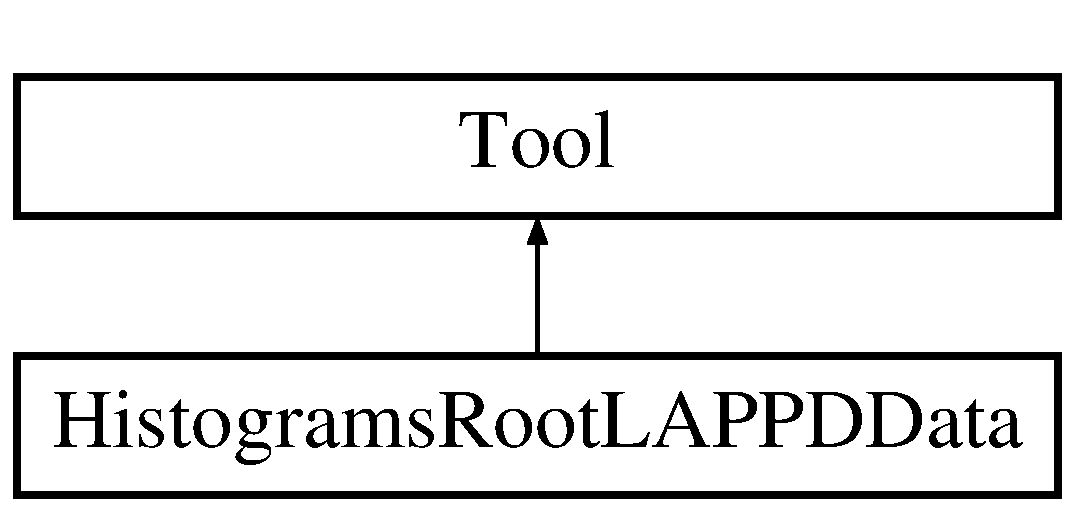
\includegraphics[height=2.000000cm]{classHistogramsRootLAPPDData}
\end{center}
\end{figure}
\subsection*{Public Member Functions}
\begin{DoxyCompactItemize}
\item 
\hypertarget{classHistogramsRootLAPPDData_ab87ee19ac23e1a888976464ec0e9b199}{bool {\bfseries Initialise} (std\-::string configfile, \hyperlink{classDataModel}{Data\-Model} \&data)}\label{classHistogramsRootLAPPDData_ab87ee19ac23e1a888976464ec0e9b199}

\item 
\hypertarget{classHistogramsRootLAPPDData_a81c098fc773fb9bb365beb47aefd67d7}{bool {\bfseries Execute} ()}\label{classHistogramsRootLAPPDData_a81c098fc773fb9bb365beb47aefd67d7}

\item 
\hypertarget{classHistogramsRootLAPPDData_abc484166b3afed20afc9a702c3a003da}{bool {\bfseries Finalise} ()}\label{classHistogramsRootLAPPDData_abc484166b3afed20afc9a702c3a003da}

\end{DoxyCompactItemize}


The documentation for this class was generated from the following file\-:\begin{DoxyCompactItemize}
\item 
User\-Tools/\-Histograms\-Root\-L\-A\-P\-P\-D\-Data/Histograms\-Root\-L\-A\-P\-P\-D\-Data.\-h\end{DoxyCompactItemize}

\hypertarget{classHit}{\section{Hit Class Reference}
\label{classHit}\index{Hit@{Hit}}
}
Inheritance diagram for Hit\-:\begin{figure}[H]
\begin{center}
\leavevmode
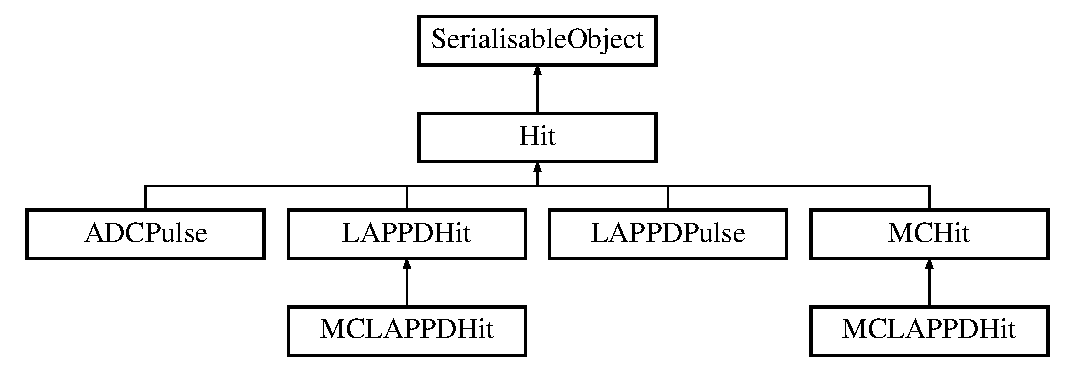
\includegraphics[height=4.000000cm]{classHit}
\end{center}
\end{figure}
\subsection*{Public Member Functions}
\begin{DoxyCompactItemize}
\item 
\hypertarget{classHit_a46c21425b896c5638598b4116de73740}{{\bfseries Hit} (int thetubeid, double thetime, double thecharge)}\label{classHit_a46c21425b896c5638598b4116de73740}

\item 
\hypertarget{classHit_ad4da9c11c8a203b65bd8b97b144a8133}{int {\bfseries Get\-Tube\-Id} () const }\label{classHit_ad4da9c11c8a203b65bd8b97b144a8133}

\item 
\hypertarget{classHit_aa67ab762ecf9eab3d41147667447c597}{double {\bfseries Get\-Time} () const }\label{classHit_aa67ab762ecf9eab3d41147667447c597}

\item 
\hypertarget{classHit_a77e2a2c8ed9449b38fc00e1d516d122a}{double {\bfseries Get\-Charge} () const }\label{classHit_a77e2a2c8ed9449b38fc00e1d516d122a}

\item 
\hypertarget{classHit_a2f1d81f94c9cfc35ba664b94fd719156}{void {\bfseries Set\-Tube\-Id} (int tubeid)}\label{classHit_a2f1d81f94c9cfc35ba664b94fd719156}

\item 
\hypertarget{classHit_af540ccdede0608cdd9ce6e754258b5e8}{void {\bfseries Set\-Time} (double tc)}\label{classHit_af540ccdede0608cdd9ce6e754258b5e8}

\item 
\hypertarget{classHit_aabbc33179a273289414263478835f2b9}{void {\bfseries Set\-Charge} (double chg)}\label{classHit_aabbc33179a273289414263478835f2b9}

\item 
\hypertarget{classHit_acebd1b0fb425a531faefed955f4c87e2}{bool {\bfseries Print} ()}\label{classHit_acebd1b0fb425a531faefed955f4c87e2}

\end{DoxyCompactItemize}
\subsection*{Protected Member Functions}
\begin{DoxyCompactItemize}
\item 
\hypertarget{classHit_af3bafb22cc7c2c224af22927c6ea2d07}{{\footnotesize template$<$class Archive $>$ }\\void {\bfseries serialize} (Archive \&ar, const unsigned int version)}\label{classHit_af3bafb22cc7c2c224af22927c6ea2d07}

\end{DoxyCompactItemize}
\subsection*{Protected Attributes}
\begin{DoxyCompactItemize}
\item 
\hypertarget{classHit_a442f7a2eebdfbc0e8c29194f4e26e40e}{int {\bfseries Tube\-Id}}\label{classHit_a442f7a2eebdfbc0e8c29194f4e26e40e}

\item 
\hypertarget{classHit_a8abba0e32e50c99ed70f38f660486e29}{double {\bfseries Time}}\label{classHit_a8abba0e32e50c99ed70f38f660486e29}

\item 
\hypertarget{classHit_a6460be8aae8df3d04ae3871d99bf0193}{double {\bfseries Charge}}\label{classHit_a6460be8aae8df3d04ae3871d99bf0193}

\end{DoxyCompactItemize}
\subsection*{Friends}
\begin{DoxyCompactItemize}
\item 
\hypertarget{classHit_ac98d07dd8f7b70e16ccb9a01abf56b9c}{class {\bfseries boost\-::serialization\-::access}}\label{classHit_ac98d07dd8f7b70e16ccb9a01abf56b9c}

\end{DoxyCompactItemize}


The documentation for this class was generated from the following file\-:\begin{DoxyCompactItemize}
\item 
Data\-Model/Hit.\-h\end{DoxyCompactItemize}

\hypertarget{classHitCleaner}{
\section{HitCleaner Class Reference}
\label{classHitCleaner}\index{HitCleaner@{HitCleaner}}
}
\subsection*{Public Types}
\begin{DoxyCompactItemize}
\item 
enum {\bfseries EFilterConfig} \{ \par
{\bfseries kNone} =  0, 
{\bfseries kPulseHeight} =  1, 
{\bfseries kPulseHeightAndNeighbours} =  2, 
{\bfseries kPulseHeightAndClusters} =  3, 
\par
{\bfseries kPulseHeightAndTruthInfo} =  3
 \}
\item 
\hypertarget{classHitCleaner_a417732ebe6c9a62f91a0648522cb5e01}{
typedef enum HitCleaner::EFilterConfig {\bfseries FilterConfig\_\-t}}
\label{classHitCleaner_a417732ebe6c9a62f91a0648522cb5e01}

\end{DoxyCompactItemize}
\subsection*{Public Member Functions}
\begin{DoxyCompactItemize}
\item 
bool \hyperlink{classHitCleaner_a35bd6ca1401c52439166e51c7e873ace}{Initialise} (std::string configfile, \hyperlink{classDataModel}{DataModel} \&data)
\item 
bool \hyperlink{classHitCleaner_adec5b94400dcbfc710590d7eb387041b}{Execute} ()
\item 
\hypertarget{classHitCleaner_a06d16e3d574ec685952c011d2309fa76}{
bool {\bfseries Finalise} ()}
\label{classHitCleaner_a06d16e3d574ec685952c011d2309fa76}

\item 
\hypertarget{classHitCleaner_a2d7f24be0dae3a9aa53771bc0bdb65c6}{
void {\bfseries PrintParameters} ()}
\label{classHitCleaner_a2d7f24be0dae3a9aa53771bc0bdb65c6}

\item 
\hypertarget{classHitCleaner_af75191aadcf2acffcc1c13549d062fc8}{
void {\bfseries SetConfig} (int config)}
\label{classHitCleaner_af75191aadcf2acffcc1c13549d062fc8}

\item 
\hypertarget{classHitCleaner_acb667165fb7166a54b5401264c76cf60}{
void {\bfseries SetPmtMinPulseHeight} (double min)}
\label{classHitCleaner_acb667165fb7166a54b5401264c76cf60}

\item 
\hypertarget{classHitCleaner_a48ecb1833030a1e53d76f852735b1146}{
void {\bfseries SetPmtNeighbourRadius} (double radius)}
\label{classHitCleaner_a48ecb1833030a1e53d76f852735b1146}

\item 
\hypertarget{classHitCleaner_a05aaf25ef5464e2cc0cbb67a123a4683}{
void {\bfseries SetPmtNeighbourDigits} (int digits)}
\label{classHitCleaner_a05aaf25ef5464e2cc0cbb67a123a4683}

\item 
\hypertarget{classHitCleaner_a374f2c25fd741ba89253c1df57c2f711}{
void {\bfseries SetPmtClusterRadius} (double radius)}
\label{classHitCleaner_a374f2c25fd741ba89253c1df57c2f711}

\item 
\hypertarget{classHitCleaner_a2034dc5fabc9bd6a7f06bfe9be9172f4}{
void {\bfseries SetPmtTimeWindowNeighbours} (double windowN)}
\label{classHitCleaner_a2034dc5fabc9bd6a7f06bfe9be9172f4}

\item 
\hypertarget{classHitCleaner_a5d427dd83732333d8918993e2c5a08d2}{
void {\bfseries SetPmtTimeWindowClusters} (double windowC)}
\label{classHitCleaner_a5d427dd83732333d8918993e2c5a08d2}

\item 
\hypertarget{classHitCleaner_abe7877bee548ff2e72db4991ebe8d9b1}{
void {\bfseries SetLappdMinPulseHeight} (double min)}
\label{classHitCleaner_abe7877bee548ff2e72db4991ebe8d9b1}

\item 
\hypertarget{classHitCleaner_a3deef1a55f3597115b7a1514c23ab2b4}{
void {\bfseries SetLappdNeighbourRadius} (double radius)}
\label{classHitCleaner_a3deef1a55f3597115b7a1514c23ab2b4}

\item 
\hypertarget{classHitCleaner_af872da7d231440f4fa75b2dfe6be5fc8}{
void {\bfseries SetLappdNeighbourDigits} (int digits)}
\label{classHitCleaner_af872da7d231440f4fa75b2dfe6be5fc8}

\item 
\hypertarget{classHitCleaner_aacf88b73ee3bb0bb4afa4648c64add65}{
void {\bfseries SetLappdClusterRadius} (double radius)}
\label{classHitCleaner_aacf88b73ee3bb0bb4afa4648c64add65}

\item 
\hypertarget{classHitCleaner_aaa0aca2da3c1a4670e9a4a1361e9b124}{
void {\bfseries SetLappdTimeWindowNeighbours} (double windowN)}
\label{classHitCleaner_aaa0aca2da3c1a4670e9a4a1361e9b124}

\item 
\hypertarget{classHitCleaner_a093989b06deb5743b6c4c81092e69ceb}{
void {\bfseries SetLappdTimeWindowClusters} (double windowC)}
\label{classHitCleaner_a093989b06deb5743b6c4c81092e69ceb}

\item 
\hypertarget{classHitCleaner_a6f25436f395cb868857f7a4b5c418de2}{
void {\bfseries LoadConfigFile} (string configfilename)}
\label{classHitCleaner_a6f25436f395cb868857f7a4b5c418de2}

\item 
\hypertarget{classHitCleaner_a1154c24324e11dc8d0d53bcd806d7113}{
void {\bfseries SetMinClusterDigits} (int digits)}
\label{classHitCleaner_a1154c24324e11dc8d0d53bcd806d7113}

\item 
\hypertarget{classHitCleaner_ae47191a46b30d5345b1e1c422767f816}{
std::vector$<$ \hyperlink{classRecoDigit}{RecoDigit} $\ast$ $>$ $\ast$ {\bfseries Run} (std::vector$<$ \hyperlink{classRecoDigit}{RecoDigit} $\ast$ $>$ $\ast$digitlist)}
\label{classHitCleaner_ae47191a46b30d5345b1e1c422767f816}

\item 
\hypertarget{classHitCleaner_a3c85370ccb39e1615976fe4acb218fb5}{
std::vector$<$ \hyperlink{classRecoDigit}{RecoDigit} $\ast$ $>$ $\ast$ {\bfseries ResetDigits} (std::vector$<$ \hyperlink{classRecoDigit}{RecoDigit} $\ast$ $>$ $\ast$digitlist)}
\label{classHitCleaner_a3c85370ccb39e1615976fe4acb218fb5}

\item 
\hypertarget{classHitCleaner_a16028ae7a55a4cdcfdb116af893d2542}{
std::vector$<$ \hyperlink{classRecoDigit}{RecoDigit} $\ast$ $>$ $\ast$ {\bfseries FilterDigits} (std::vector$<$ \hyperlink{classRecoDigit}{RecoDigit} $\ast$ $>$ $\ast$digitlist)}
\label{classHitCleaner_a16028ae7a55a4cdcfdb116af893d2542}

\item 
\hypertarget{classHitCleaner_a7e6188a785adddfcaa3dbe63de387e95}{
std::vector$<$ \hyperlink{classRecoDigit}{RecoDigit} $\ast$ $>$ $\ast$ {\bfseries FilterAll} (std::vector$<$ \hyperlink{classRecoDigit}{RecoDigit} $\ast$ $>$ $\ast$digitlist)}
\label{classHitCleaner_a7e6188a785adddfcaa3dbe63de387e95}

\item 
\hypertarget{classHitCleaner_a537c7f9b371c0dc52df86046f8a90336}{
std::vector$<$ \hyperlink{classRecoDigit}{RecoDigit} $\ast$ $>$ $\ast$ {\bfseries FilterByPulseHeight} (std::vector$<$ \hyperlink{classRecoDigit}{RecoDigit} $\ast$ $>$ $\ast$digitlist)}
\label{classHitCleaner_a537c7f9b371c0dc52df86046f8a90336}

\item 
\hypertarget{classHitCleaner_ad574e2c8d1718971cbfce2a284731daa}{
std::vector$<$ \hyperlink{classRecoDigit}{RecoDigit} $\ast$ $>$ $\ast$ {\bfseries FilterByNeighbours} (std::vector$<$ \hyperlink{classRecoDigit}{RecoDigit} $\ast$ $>$ $\ast$digitlist)}
\label{classHitCleaner_ad574e2c8d1718971cbfce2a284731daa}

\item 
\hypertarget{classHitCleaner_a32e29edc8c7564e423186efacbea07c5}{
std::vector$<$ \hyperlink{classRecoDigit}{RecoDigit} $\ast$ $>$ $\ast$ {\bfseries FilterByClusters} (std::vector$<$ \hyperlink{classRecoDigit}{RecoDigit} $\ast$ $>$ $\ast$digitlist)}
\label{classHitCleaner_a32e29edc8c7564e423186efacbea07c5}

\item 
\hypertarget{classHitCleaner_ad2c117045b0a63c700b0f2a94f3fa0b2}{
std::vector$<$ \hyperlink{classRecoDigit}{RecoDigit} $\ast$ $>$ $\ast$ {\bfseries FilterByTruthInfo} (std::vector$<$ \hyperlink{classRecoDigit}{RecoDigit} $\ast$ $>$ $\ast$digitlist)}
\label{classHitCleaner_ad2c117045b0a63c700b0f2a94f3fa0b2}

\item 
\hypertarget{classHitCleaner_a0e516802fcbaad1e3e61978911991949}{
std::vector$<$ \hyperlink{classRecoCluster}{RecoCluster} $\ast$ $>$ $\ast$ {\bfseries RecoClusters} (std::vector$<$ \hyperlink{classRecoDigit}{RecoDigit} $\ast$ $>$ $\ast$digitlist)}
\label{classHitCleaner_a0e516802fcbaad1e3e61978911991949}

\end{DoxyCompactItemize}
\subsection*{Static Public Member Functions}
\begin{DoxyCompactItemize}
\item 
\hypertarget{classHitCleaner_a4ac1bde4eec18c427ed249409a6d5d3a}{
static \hyperlink{classHitCleaner}{HitCleaner} $\ast$ {\bfseries Instance} ()}
\label{classHitCleaner_a4ac1bde4eec18c427ed249409a6d5d3a}

\item 
\hypertarget{classHitCleaner_afdf345b322cbef82deb9f35eaddb02d1}{
static void {\bfseries Config} (int config)}
\label{classHitCleaner_afdf345b322cbef82deb9f35eaddb02d1}

\item 
\hypertarget{classHitCleaner_a94987b09a59d9781277f76eee63994a1}{
static void {\bfseries PmtMinPulseHeight} (double min)}
\label{classHitCleaner_a94987b09a59d9781277f76eee63994a1}

\item 
\hypertarget{classHitCleaner_af6d017ac189b0eb6abf064756e78f5ac}{
static void {\bfseries PmtNeighbourRadius} (double radius)}
\label{classHitCleaner_af6d017ac189b0eb6abf064756e78f5ac}

\item 
\hypertarget{classHitCleaner_a43b5a1ac75e62334a8e9ff539a9b34df}{
static void {\bfseries PmtNeighbourDigits} (int digits)}
\label{classHitCleaner_a43b5a1ac75e62334a8e9ff539a9b34df}

\item 
\hypertarget{classHitCleaner_a71881188d23e57c9afb0c8179ff9c5e3}{
static void {\bfseries PmtClusterRadius} (double radius)}
\label{classHitCleaner_a71881188d23e57c9afb0c8179ff9c5e3}

\item 
\hypertarget{classHitCleaner_a8074ae3702ee872e8c8b4504f3bf3987}{
static void {\bfseries MinClusterDigits} (int digits)}
\label{classHitCleaner_a8074ae3702ee872e8c8b4504f3bf3987}

\item 
\hypertarget{classHitCleaner_a2efa2634319c4ff56e51ba28415146a9}{
static void {\bfseries PmtTimeWindowN} (double windowN)}
\label{classHitCleaner_a2efa2634319c4ff56e51ba28415146a9}

\item 
\hypertarget{classHitCleaner_a1962dfdb70798529f8f560c1b6f233fc}{
static void {\bfseries PmtTimeWindowC} (double windowC)}
\label{classHitCleaner_a1962dfdb70798529f8f560c1b6f233fc}

\end{DoxyCompactItemize}


\subsection{Member Function Documentation}
\hypertarget{classHitCleaner_adec5b94400dcbfc710590d7eb387041b}{
\index{HitCleaner@{HitCleaner}!Execute@{Execute}}
\index{Execute@{Execute}!HitCleaner@{HitCleaner}}
\subsubsection[{Execute}]{\setlength{\rightskip}{0pt plus 5cm}bool HitCleaner::Execute ()}}
\label{classHitCleaner_adec5b94400dcbfc710590d7eb387041b}


see if \char`\"{}RecoEvent\char`\"{} exists

$>$ Get digits from \char`\"{}RecoEvent\char`\"{} \hypertarget{classHitCleaner_a35bd6ca1401c52439166e51c7e873ace}{
\index{HitCleaner@{HitCleaner}!Initialise@{Initialise}}
\index{Initialise@{Initialise}!HitCleaner@{HitCleaner}}
\subsubsection[{Initialise}]{\setlength{\rightskip}{0pt plus 5cm}bool HitCleaner::Initialise (std::string {\em configfile}, \/  {\bf DataModel} \& {\em data})}}
\label{classHitCleaner_a35bd6ca1401c52439166e51c7e873ace}


Get the Tool configuration variables 

The documentation for this class was generated from the following files:\begin{DoxyCompactItemize}
\item 
UserTools/HitCleaner/HitCleaner.h\item 
UserTools/HitCleaner/HitCleaner.cpp\end{DoxyCompactItemize}

\hypertarget{classHitResiduals}{\section{Hit\-Residuals Class Reference}
\label{classHitResiduals}\index{Hit\-Residuals@{Hit\-Residuals}}
}
Inheritance diagram for Hit\-Residuals\-:\begin{figure}[H]
\begin{center}
\leavevmode
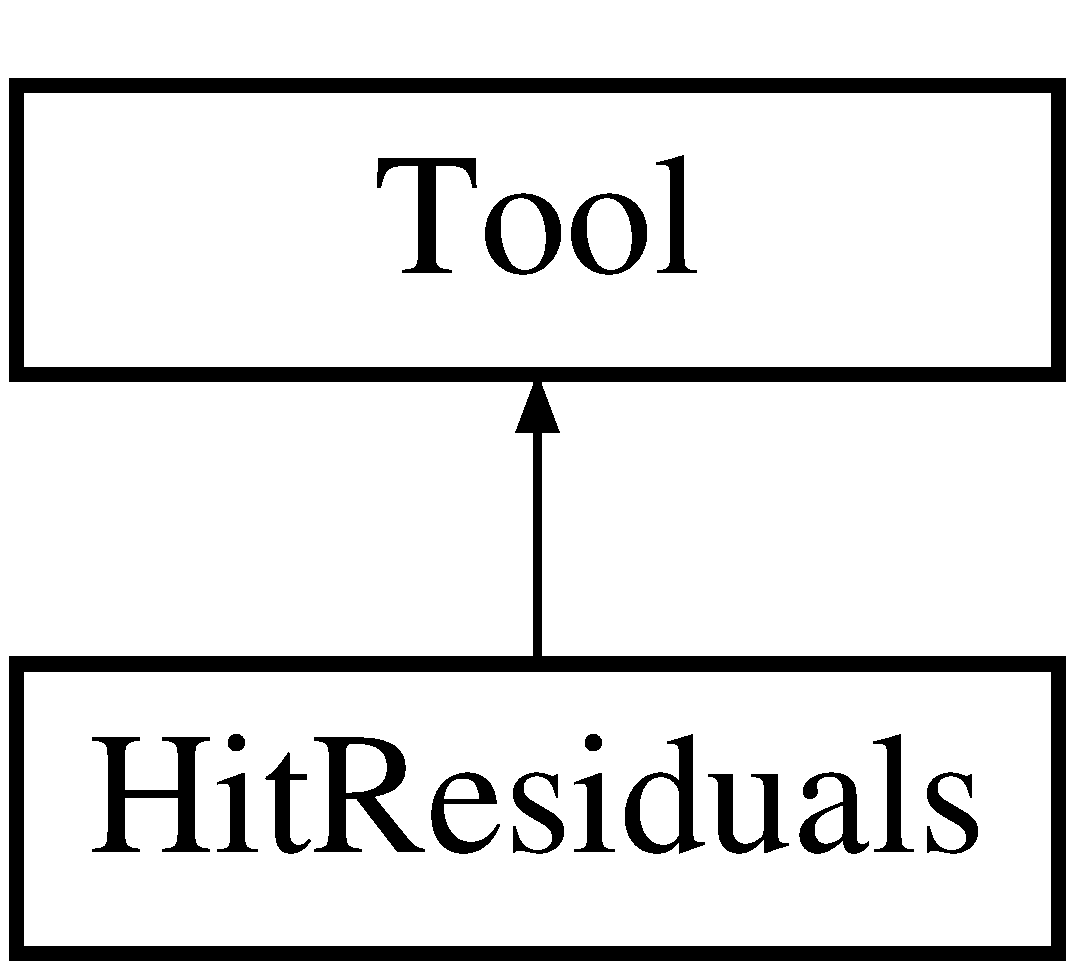
\includegraphics[height=2.000000cm]{classHitResiduals}
\end{center}
\end{figure}
\subsection*{Public Member Functions}
\begin{DoxyCompactItemize}
\item 
\hypertarget{classHitResiduals_ac37e7a71c2fece45c304383ace201de8}{bool {\bfseries Initialise} (std\-::string configfile, \hyperlink{classDataModel}{Data\-Model} \&data)}\label{classHitResiduals_ac37e7a71c2fece45c304383ace201de8}

\item 
\hypertarget{classHitResiduals_a6715e864b1c07e812178cc0d3b245339}{bool {\bfseries Execute} ()}\label{classHitResiduals_a6715e864b1c07e812178cc0d3b245339}

\item 
\hypertarget{classHitResiduals_a00c3b75308417bfd468cbb786104c26f}{bool {\bfseries Finalise} ()}\label{classHitResiduals_a00c3b75308417bfd468cbb786104c26f}

\end{DoxyCompactItemize}


The documentation for this class was generated from the following files\-:\begin{DoxyCompactItemize}
\item 
User\-Tools/\-Hit\-Residuals/Hit\-Residuals.\-h\item 
User\-Tools/\-Hit\-Residuals/Hit\-Residuals.\-cpp\end{DoxyCompactItemize}

\hypertarget{classIFBeamDBInterface}{\section{I\-F\-Beam\-D\-B\-Interface Class Reference}
\label{classIFBeamDBInterface}\index{I\-F\-Beam\-D\-B\-Interface@{I\-F\-Beam\-D\-B\-Interface}}
}


Singleton used to interact with the Intensity Frontier beam database at Fermilab.  




{\ttfamily \#include $<$I\-F\-Beam\-D\-B\-Interface.\-h$>$}

\subsection*{Public Member Functions}
\begin{DoxyCompactItemize}
\item 
\hypertarget{classIFBeamDBInterface_ac6e95cfed4db9c455289234f26a2f1c1}{\hyperlink{classIFBeamDBInterface_ac6e95cfed4db9c455289234f26a2f1c1}{$\sim$\-I\-F\-Beam\-D\-B\-Interface} ()}\label{classIFBeamDBInterface_ac6e95cfed4db9c455289234f26a2f1c1}

\begin{DoxyCompactList}\small\item\em Clean up libcurl stuff as the \hyperlink{classIFBeamDBInterface}{I\-F\-Beam\-D\-B\-Interface} object is destroyed. \end{DoxyCompactList}\item 
\hypertarget{classIFBeamDBInterface_aac246a02f0726c599a8bd6db201c9c81}{\hyperlink{classIFBeamDBInterface_aac246a02f0726c599a8bd6db201c9c81}{I\-F\-Beam\-D\-B\-Interface} (const \hyperlink{classIFBeamDBInterface}{I\-F\-Beam\-D\-B\-Interface} \&)=delete}\label{classIFBeamDBInterface_aac246a02f0726c599a8bd6db201c9c81}

\begin{DoxyCompactList}\small\item\em Deleted copy constructor. \end{DoxyCompactList}\item 
\hypertarget{classIFBeamDBInterface_ae53bfb59f783375aeb96e520e1b8a4c8}{\hyperlink{classIFBeamDBInterface_ae53bfb59f783375aeb96e520e1b8a4c8}{I\-F\-Beam\-D\-B\-Interface} (\hyperlink{classIFBeamDBInterface}{I\-F\-Beam\-D\-B\-Interface} \&\&)=delete}\label{classIFBeamDBInterface_ae53bfb59f783375aeb96e520e1b8a4c8}

\begin{DoxyCompactList}\small\item\em Deleted move constructor. \end{DoxyCompactList}\item 
\hypertarget{classIFBeamDBInterface_ad3af28661e5c86ba91c795f841678188}{\hyperlink{classIFBeamDBInterface}{I\-F\-Beam\-D\-B\-Interface} \& \hyperlink{classIFBeamDBInterface_ad3af28661e5c86ba91c795f841678188}{operator=} (const \hyperlink{classIFBeamDBInterface}{I\-F\-Beam\-D\-B\-Interface} \&)=delete}\label{classIFBeamDBInterface_ad3af28661e5c86ba91c795f841678188}

\begin{DoxyCompactList}\small\item\em Deleted copy assignment operator. \end{DoxyCompactList}\item 
\hypertarget{classIFBeamDBInterface_adbdd5916724ed8747b0e6ca705e07184}{\hyperlink{classIFBeamDBInterface}{I\-F\-Beam\-D\-B\-Interface} \& \hyperlink{classIFBeamDBInterface_adbdd5916724ed8747b0e6ca705e07184}{operator=} (\hyperlink{classIFBeamDBInterface}{I\-F\-Beam\-D\-B\-Interface} \&\&)=delete}\label{classIFBeamDBInterface_adbdd5916724ed8747b0e6ca705e07184}

\begin{DoxyCompactList}\small\item\em Deleted move assignment operator. \end{DoxyCompactList}\item 
std\-::map$<$ std\-::string, \\*
std\-::map$<$ uint64\-\_\-t, \\*
\hyperlink{structBeamDataPoint}{Beam\-Data\-Point} $>$ $>$ \hyperlink{classIFBeamDBInterface_a7b0e4c42767791f1904540b63772a74d}{Query\-Beam\-D\-B} (uint64\-\_\-t t0, uint64\-\_\-t t1) const 
\begin{DoxyCompactList}\small\item\em Get information about the Booster Neutrino Beam (B\-N\-B) state from the database for the time interval \mbox{[}t0, t1\mbox{]}. \end{DoxyCompactList}\item 
int \hyperlink{classIFBeamDBInterface_a034ef023cb78989270a4ec2d54a5aa4f}{Query\-Beam\-D\-B} (uint64\-\_\-t t0, uint64\-\_\-t t1, std\-::string \&response\-\_\-string) const 
\begin{DoxyCompactList}\small\item\em Get information about the B\-N\-B state from the database for the time interval \mbox{[}t0, t1\mbox{]}. \end{DoxyCompactList}\item 
\hyperlink{classBeamStatus}{Beam\-Status} \hyperlink{classIFBeamDBInterface_add525c53cbf0b85c3cd0d39a5b9b0fdd}{Get\-Beam\-Status} (uint64\-\_\-t time) const 
\begin{DoxyCompactList}\small\item\em Get information about the B\-N\-B state from the database as close as possible to a given time. \end{DoxyCompactList}\end{DoxyCompactItemize}
\subsection*{Static Public Member Functions}
\begin{DoxyCompactItemize}
\item 
\hypertarget{classIFBeamDBInterface_a677ed1a3b7dbfc70ffb0688078ae5fb0}{static const \hyperlink{classIFBeamDBInterface}{I\-F\-Beam\-D\-B\-Interface} \& \hyperlink{classIFBeamDBInterface_a677ed1a3b7dbfc70ffb0688078ae5fb0}{Instance} ()}\label{classIFBeamDBInterface_a677ed1a3b7dbfc70ffb0688078ae5fb0}

\begin{DoxyCompactList}\small\item\em Get a const reference to the singleton instance of the \hyperlink{classIFBeamDBInterface}{I\-F\-Beam\-D\-B\-Interface}. \end{DoxyCompactList}\end{DoxyCompactItemize}
\subsection*{Protected Member Functions}
\begin{DoxyCompactItemize}
\item 
\hypertarget{classIFBeamDBInterface_af5275e528b9b43d4c5dacd0a8a3ca62b}{\hyperlink{classIFBeamDBInterface_af5275e528b9b43d4c5dacd0a8a3ca62b}{I\-F\-Beam\-D\-B\-Interface} ()}\label{classIFBeamDBInterface_af5275e528b9b43d4c5dacd0a8a3ca62b}

\begin{DoxyCompactList}\small\item\em Create the singleton \hyperlink{classIFBeamDBInterface}{I\-F\-Beam\-D\-B\-Interface} object. \end{DoxyCompactList}\item 
\hypertarget{classIFBeamDBInterface_a950bec54fb41eaf48471a8a1eab8ab71}{std\-::map$<$ std\-::string, \\*
std\-::map$<$ uint64\-\_\-t, \\*
\hyperlink{structBeamDataPoint}{Beam\-Data\-Point} $>$ $>$ {\bfseries Parse\-D\-B\-Response} (const std\-::string \&response) const }\label{classIFBeamDBInterface_a950bec54fb41eaf48471a8a1eab8ab71}

\item 
\hypertarget{classIFBeamDBInterface_a2d7b151e8b21fe5f7d255d442d37e321}{void {\bfseries Postprocess\-Parsed\-Response} (std\-::map$<$ std\-::string, std\-::map$<$ uint64\-\_\-t, \hyperlink{structBeamDataPoint}{Beam\-Data\-Point} $>$ $>$ \&parsed\-\_\-response) const }\label{classIFBeamDBInterface_a2d7b151e8b21fe5f7d255d442d37e321}

\end{DoxyCompactItemize}
\subsection*{Protected Attributes}
\begin{DoxyCompactItemize}
\item 
\hypertarget{classIFBeamDBInterface_a7dea07c539e0f0ca765f02d198345d2d}{C\-U\-R\-L $\ast$ \hyperlink{classIFBeamDBInterface_a7dea07c539e0f0ca765f02d198345d2d}{f\-Curl} = nullptr}\label{classIFBeamDBInterface_a7dea07c539e0f0ca765f02d198345d2d}

\begin{DoxyCompactList}\small\item\em Pointer used to interact with libcurl. \end{DoxyCompactList}\end{DoxyCompactItemize}


\subsection{Detailed Description}
Singleton used to interact with the Intensity Frontier beam database at Fermilab. 

\subsection{Member Function Documentation}
\hypertarget{classIFBeamDBInterface_add525c53cbf0b85c3cd0d39a5b9b0fdd}{\index{I\-F\-Beam\-D\-B\-Interface@{I\-F\-Beam\-D\-B\-Interface}!Get\-Beam\-Status@{Get\-Beam\-Status}}
\index{Get\-Beam\-Status@{Get\-Beam\-Status}!IFBeamDBInterface@{I\-F\-Beam\-D\-B\-Interface}}
\subsubsection[{Get\-Beam\-Status}]{\setlength{\rightskip}{0pt plus 5cm}{\bf Beam\-Status} I\-F\-Beam\-D\-B\-Interface\-::\-Get\-Beam\-Status (
\begin{DoxyParamCaption}
\item[{uint64\-\_\-t}]{time}
\end{DoxyParamCaption}
) const}}\label{classIFBeamDBInterface_add525c53cbf0b85c3cd0d39a5b9b0fdd}


Get information about the B\-N\-B state from the database as close as possible to a given time. 


\begin{DoxyParams}{Parameters}
{\em time} & Timestamp (milliseconds since the Unix epoch) to use when searching the database \\
\hline
\end{DoxyParams}
\hypertarget{classIFBeamDBInterface_a7b0e4c42767791f1904540b63772a74d}{\index{I\-F\-Beam\-D\-B\-Interface@{I\-F\-Beam\-D\-B\-Interface}!Query\-Beam\-D\-B@{Query\-Beam\-D\-B}}
\index{Query\-Beam\-D\-B@{Query\-Beam\-D\-B}!IFBeamDBInterface@{I\-F\-Beam\-D\-B\-Interface}}
\subsubsection[{Query\-Beam\-D\-B}]{\setlength{\rightskip}{0pt plus 5cm}std\-::map$<$ std\-::string, std\-::map$<$ uint64\-\_\-t, {\bf Beam\-Data\-Point} $>$ $>$ I\-F\-Beam\-D\-B\-Interface\-::\-Query\-Beam\-D\-B (
\begin{DoxyParamCaption}
\item[{uint64\-\_\-t}]{t0, }
\item[{uint64\-\_\-t}]{t1}
\end{DoxyParamCaption}
) const}}\label{classIFBeamDBInterface_a7b0e4c42767791f1904540b63772a74d}


Get information about the Booster Neutrino Beam (B\-N\-B) state from the database for the time interval \mbox{[}t0, t1\mbox{]}. 

\begin{DoxyVerb}@param t0 Starting timestamp (milliseconds since the Unix epoch)
@param t1 Starting timestamp (milliseconds since the Unix epoch)
@return A nested map containing the parsed data. Keys of the outer map
are device names, values are inner maps. Keys of the inner map are
timestamps (milliseconds since the Unix epoch), values are
BeamDataPoint structs that hold a numerical value and a unit string.
@note An easy way to get the current milliseconds since the Unix epoch
is to use the terminal utility date like this:@verbatim date +%s%3N
\end{DoxyVerb}
 ///  I found this handy trick here\-: \href{http://unix.stackexchange.com/a/123764}{\tt http\-://unix.\-stackexchange.\-com/a/123764} \hypertarget{classIFBeamDBInterface_a034ef023cb78989270a4ec2d54a5aa4f}{\index{I\-F\-Beam\-D\-B\-Interface@{I\-F\-Beam\-D\-B\-Interface}!Query\-Beam\-D\-B@{Query\-Beam\-D\-B}}
\index{Query\-Beam\-D\-B@{Query\-Beam\-D\-B}!IFBeamDBInterface@{I\-F\-Beam\-D\-B\-Interface}}
\subsubsection[{Query\-Beam\-D\-B}]{\setlength{\rightskip}{0pt plus 5cm}int I\-F\-Beam\-D\-B\-Interface\-::\-Query\-Beam\-D\-B (
\begin{DoxyParamCaption}
\item[{uint64\-\_\-t}]{t0, }
\item[{uint64\-\_\-t}]{t1, }
\item[{std\-::string \&}]{response\-\_\-string}
\end{DoxyParamCaption}
) const}}\label{classIFBeamDBInterface_a034ef023cb78989270a4ec2d54a5aa4f}


Get information about the B\-N\-B state from the database for the time interval \mbox{[}t0, t1\mbox{]}. 


\begin{DoxyParams}[1]{Parameters}
 & {\em t0} & Starting timestamp (milliseconds since the Unix epoch) \\
\hline
 & {\em t1} & Starting timestamp (milliseconds since the Unix epoch) \\
\hline
\mbox{\tt out}  & {\em response\-\_\-string} & A string that will be loaded with the csv-\/format data from the database \\
\hline
\end{DoxyParams}
\begin{DoxyReturn}{Returns}
The libcurl integer return code for the query (zero if everything worked ok, or nonzero if an error occurred) 
\end{DoxyReturn}


The documentation for this class was generated from the following files\-:\begin{DoxyCompactItemize}
\item 
User\-Tools/\-Beam\-Fetcher/I\-F\-Beam\-D\-B\-Interface.\-h\item 
User\-Tools/\-Beam\-Fetcher/I\-F\-Beam\-D\-B\-Interface.\-cpp\end{DoxyCompactItemize}

\hypertarget{classLAPPD}{\section{L\-A\-P\-P\-D Class Reference}
\label{classLAPPD}\index{L\-A\-P\-P\-D@{L\-A\-P\-P\-D}}
}
\subsection*{Public Member Functions}
\begin{DoxyCompactItemize}
\item 
\hypertarget{classLAPPD_a6ef9e3c05e38b61c75cd12822ab5ce98}{bool {\bfseries Print} ()}\label{classLAPPD_a6ef9e3c05e38b61c75cd12822ab5ce98}

\end{DoxyCompactItemize}
\subsection*{Public Attributes}
\begin{DoxyCompactItemize}
\item 
\hypertarget{classLAPPD_a1b6bdd53a3523932fe22ad3b5471c91b}{std\-::vector$<$ double $>$ {\bfseries waveform}}\label{classLAPPD_a1b6bdd53a3523932fe22ad3b5471c91b}

\end{DoxyCompactItemize}
\subsection*{Friends}
\begin{DoxyCompactItemize}
\item 
\hypertarget{classLAPPD_ac98d07dd8f7b70e16ccb9a01abf56b9c}{class {\bfseries boost\-::serialization\-::access}}\label{classLAPPD_ac98d07dd8f7b70e16ccb9a01abf56b9c}

\end{DoxyCompactItemize}


The documentation for this class was generated from the following file\-:\begin{DoxyCompactItemize}
\item 
Data\-Model/L\-A\-P\-P\-D.\-h\end{DoxyCompactItemize}

\hypertarget{classLAPPDAnalysis}{
\section{LAPPDAnalysis Class Reference}
\label{classLAPPDAnalysis}\index{LAPPDAnalysis@{LAPPDAnalysis}}
}
\subsection*{Public Member Functions}
\begin{DoxyCompactItemize}
\item 
\hypertarget{classLAPPDAnalysis_a3777b97151a13ebc1be6054b057b7354}{
bool {\bfseries Initialise} (std::string configfile, \hyperlink{classDataModel}{DataModel} \&data)}
\label{classLAPPDAnalysis_a3777b97151a13ebc1be6054b057b7354}

\item 
\hypertarget{classLAPPDAnalysis_a0bda0e3aa26131d460e8f11ac2d2d50d}{
bool {\bfseries Execute} ()}
\label{classLAPPDAnalysis_a0bda0e3aa26131d460e8f11ac2d2d50d}

\item 
\hypertarget{classLAPPDAnalysis_acbda60c00d2f2bceca57ff9f9098e7a7}{
bool {\bfseries Finalise} ()}
\label{classLAPPDAnalysis_acbda60c00d2f2bceca57ff9f9098e7a7}

\end{DoxyCompactItemize}


The documentation for this class was generated from the following files:\begin{DoxyCompactItemize}
\item 
UserTools/LAPPDAnalysis/LAPPDAnalysis.h\item 
UserTools/LAPPDAnalysis/LAPPDAnalysis.cpp\end{DoxyCompactItemize}

\hypertarget{classLAPPDBaselineSubtract}{
\section{LAPPDBaselineSubtract Class Reference}
\label{classLAPPDBaselineSubtract}\index{LAPPDBaselineSubtract@{LAPPDBaselineSubtract}}
}
\subsection*{Public Member Functions}
\begin{DoxyCompactItemize}
\item 
\hypertarget{classLAPPDBaselineSubtract_a9173849be0de9676949ce9e3094c0c73}{
bool {\bfseries Initialise} (std::string configfile, \hyperlink{classDataModel}{DataModel} \&data)}
\label{classLAPPDBaselineSubtract_a9173849be0de9676949ce9e3094c0c73}

\item 
\hypertarget{classLAPPDBaselineSubtract_ae2ea261ef543fa9b924a1504a250b744}{
bool {\bfseries Execute} ()}
\label{classLAPPDBaselineSubtract_ae2ea261ef543fa9b924a1504a250b744}

\item 
\hypertarget{classLAPPDBaselineSubtract_a784d6efcf77a1cb4ad27b571f3a55d8d}{
bool {\bfseries Finalise} ()}
\label{classLAPPDBaselineSubtract_a784d6efcf77a1cb4ad27b571f3a55d8d}

\end{DoxyCompactItemize}


The documentation for this class was generated from the following files:\begin{DoxyCompactItemize}
\item 
UserTools/LAPPDBaselineSubtract/LAPPDBaselineSubtract.h\item 
UserTools/LAPPDBaselineSubtract/LAPPDBaselineSubtract.cpp\end{DoxyCompactItemize}

\hypertarget{classLAPPDcfd}{\section{L\-A\-P\-P\-Dcfd Class Reference}
\label{classLAPPDcfd}\index{L\-A\-P\-P\-Dcfd@{L\-A\-P\-P\-Dcfd}}
}
Inheritance diagram for L\-A\-P\-P\-Dcfd\-:\begin{figure}[H]
\begin{center}
\leavevmode
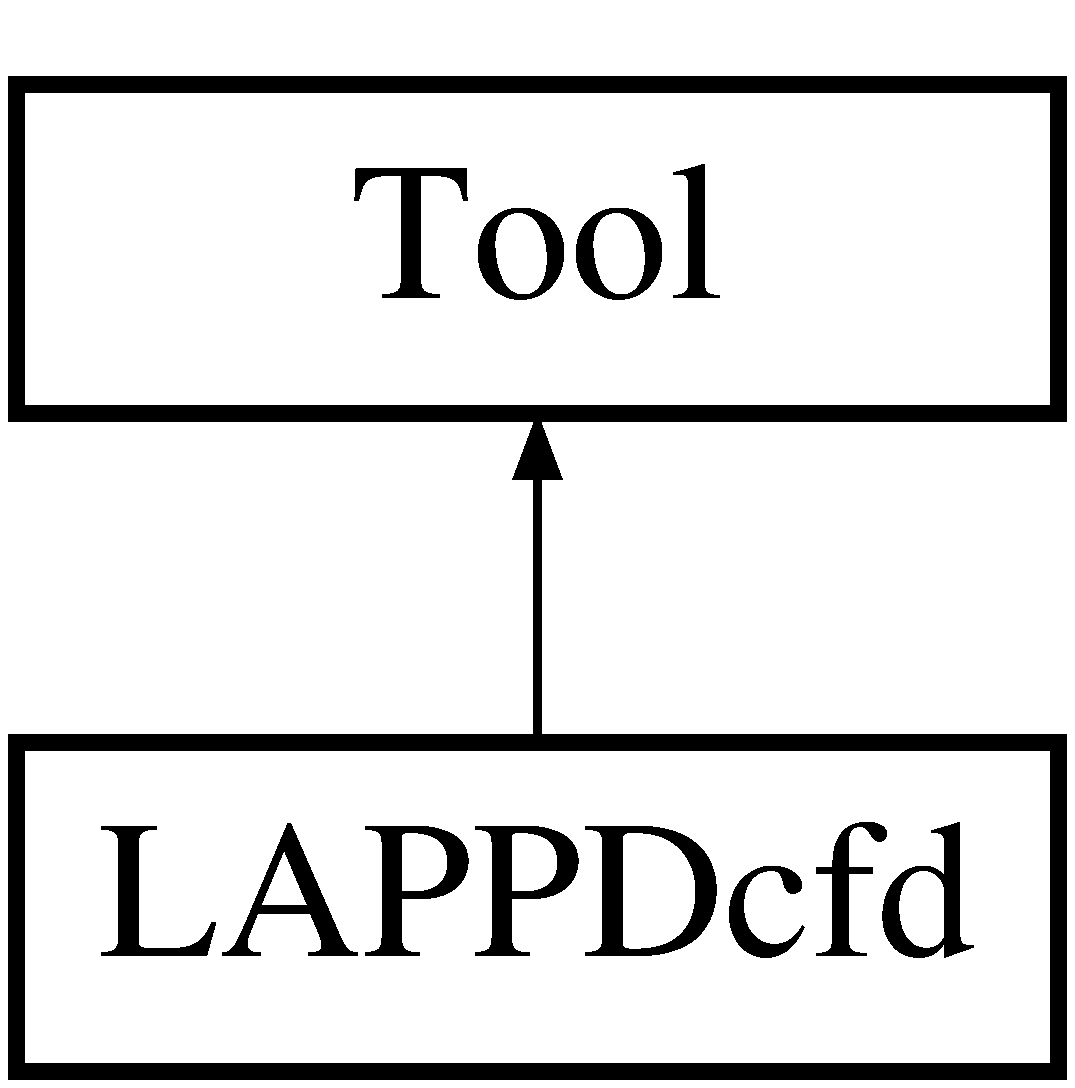
\includegraphics[height=2.000000cm]{classLAPPDcfd}
\end{center}
\end{figure}
\subsection*{Public Member Functions}
\begin{DoxyCompactItemize}
\item 
\hypertarget{classLAPPDcfd_a712d671041c6dd069c060ad9eee43b5f}{bool {\bfseries Initialise} (std\-::string configfile, \hyperlink{classDataModel}{Data\-Model} \&data)}\label{classLAPPDcfd_a712d671041c6dd069c060ad9eee43b5f}

\item 
\hypertarget{classLAPPDcfd_a7776cd36991d9ccd6ed510c58b83f765}{bool {\bfseries Execute} ()}\label{classLAPPDcfd_a7776cd36991d9ccd6ed510c58b83f765}

\item 
\hypertarget{classLAPPDcfd_a9506c223f4626d40539efd132fc21acc}{bool {\bfseries Finalise} ()}\label{classLAPPDcfd_a9506c223f4626d40539efd132fc21acc}

\item 
\hypertarget{classLAPPDcfd_a81ca5d4bda97c4e0aeb8440af918a799}{double {\bfseries C\-F\-D\-\_\-\-Discriminator1} (std\-::vector$<$ double $>$ $\ast$trace, \hyperlink{classLAPPDPulse}{L\-A\-P\-P\-D\-Pulse} pulse)}\label{classLAPPDcfd_a81ca5d4bda97c4e0aeb8440af918a799}

\item 
\hypertarget{classLAPPDcfd_a6473bfb16d498aa3ac23b566fe2a4d89}{double {\bfseries C\-F\-D\-\_\-\-Discriminator2} (std\-::vector$<$ double $>$ $\ast$trace, \hyperlink{classLAPPDPulse}{L\-A\-P\-P\-D\-Pulse} pulse)}\label{classLAPPDcfd_a6473bfb16d498aa3ac23b566fe2a4d89}

\end{DoxyCompactItemize}


The documentation for this class was generated from the following files\-:\begin{DoxyCompactItemize}
\item 
User\-Tools/\-L\-A\-P\-P\-Dcfd/L\-A\-P\-P\-Dcfd.\-h\item 
User\-Tools/\-L\-A\-P\-P\-Dcfd/L\-A\-P\-P\-Dcfd.\-cpp\end{DoxyCompactItemize}

\hypertarget{classLAPPDFilter}{
\section{LAPPDFilter Class Reference}
\label{classLAPPDFilter}\index{LAPPDFilter@{LAPPDFilter}}
}
\subsection*{Public Member Functions}
\begin{DoxyCompactItemize}
\item 
\hypertarget{classLAPPDFilter_a43acf78f4842009ea98dbea3cc8dcaee}{
bool {\bfseries Initialise} (std::string configfile, \hyperlink{classDataModel}{DataModel} \&data)}
\label{classLAPPDFilter_a43acf78f4842009ea98dbea3cc8dcaee}

\item 
\hypertarget{classLAPPDFilter_a1aea3cb930e491d79248dd24ecd703c8}{
bool {\bfseries Execute} ()}
\label{classLAPPDFilter_a1aea3cb930e491d79248dd24ecd703c8}

\item 
\hypertarget{classLAPPDFilter_a5d6a46a70be7f2320fe3fe401d3efeba}{
bool {\bfseries Finalise} ()}
\label{classLAPPDFilter_a5d6a46a70be7f2320fe3fe401d3efeba}

\end{DoxyCompactItemize}


The documentation for this class was generated from the following files:\begin{DoxyCompactItemize}
\item 
UserTools/LAPPDFilter/LAPPDFilter.h\item 
UserTools/LAPPDFilter/LAPPDFilter.cpp\end{DoxyCompactItemize}

\hypertarget{classLAPPDFindPeak}{\section{L\-A\-P\-P\-D\-Find\-Peak Class Reference}
\label{classLAPPDFindPeak}\index{L\-A\-P\-P\-D\-Find\-Peak@{L\-A\-P\-P\-D\-Find\-Peak}}
}
Inheritance diagram for L\-A\-P\-P\-D\-Find\-Peak\-:\begin{figure}[H]
\begin{center}
\leavevmode
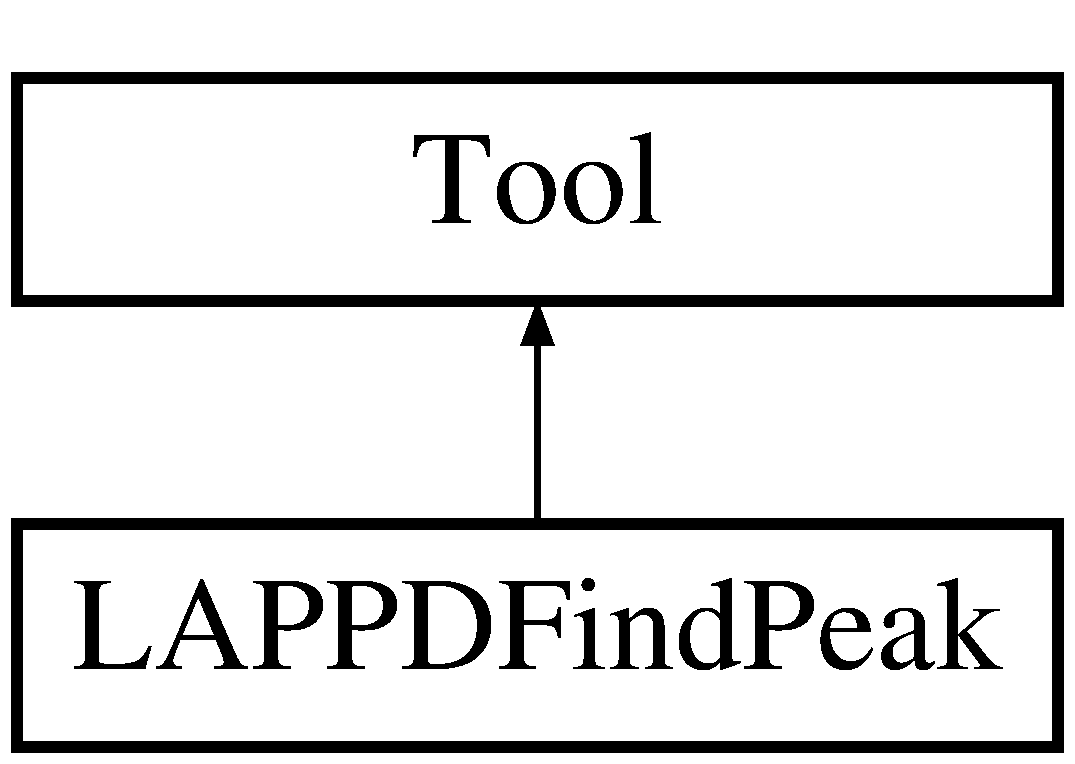
\includegraphics[height=2.000000cm]{classLAPPDFindPeak}
\end{center}
\end{figure}
\subsection*{Public Member Functions}
\begin{DoxyCompactItemize}
\item 
\hypertarget{classLAPPDFindPeak_aac02ab0efc1d6f2ac438a50a6dd48b51}{bool {\bfseries Initialise} (std\-::string configfile, \hyperlink{classDataModel}{Data\-Model} \&data)}\label{classLAPPDFindPeak_aac02ab0efc1d6f2ac438a50a6dd48b51}

\item 
\hypertarget{classLAPPDFindPeak_aeb178a0e7f0182bcec6aec80de1fd80c}{bool {\bfseries Execute} ()}\label{classLAPPDFindPeak_aeb178a0e7f0182bcec6aec80de1fd80c}

\item 
\hypertarget{classLAPPDFindPeak_a1c31ce2e8918e04c9e051a8c7eef304c}{bool {\bfseries Finalise} ()}\label{classLAPPDFindPeak_a1c31ce2e8918e04c9e051a8c7eef304c}

\item 
\hypertarget{classLAPPDFindPeak_aec4e759a18ce8bd5eda0ed4c1460ea4d}{std\-::vector$<$ \hyperlink{classLAPPDPulse}{L\-A\-P\-P\-D\-Pulse} $>$ {\bfseries Find\-Pulses\-\_\-\-T\-O\-T} (std\-::vector$<$ double $>$ $\ast$the\-Wav)}\label{classLAPPDFindPeak_aec4e759a18ce8bd5eda0ed4c1460ea4d}

\item 
\hypertarget{classLAPPDFindPeak_a705d781b236ed980dc6f6d4a297a5761}{std\-::vector$<$ \hyperlink{classLAPPDPulse}{L\-A\-P\-P\-D\-Pulse} $>$ {\bfseries Find\-Pulses\-\_\-\-Thresh} (std\-::vector$<$ double $>$ $\ast$the\-Wav)}\label{classLAPPDFindPeak_a705d781b236ed980dc6f6d4a297a5761}

\end{DoxyCompactItemize}
\subsection*{Public Attributes}
\begin{DoxyCompactItemize}
\item 
\hypertarget{classLAPPDFindPeak_a65501ad571e2fa607ba84239eab718af}{string {\bfseries Peak\-Input\-Wav\-Label}}\label{classLAPPDFindPeak_a65501ad571e2fa607ba84239eab718af}

\end{DoxyCompactItemize}


The documentation for this class was generated from the following files\-:\begin{DoxyCompactItemize}
\item 
User\-Tools/\-L\-A\-P\-P\-D\-Find\-Peak/L\-A\-P\-P\-D\-Find\-Peak.\-h\item 
User\-Tools/\-L\-A\-P\-P\-D\-Find\-Peak/L\-A\-P\-P\-D\-Find\-Peak.\-cpp\end{DoxyCompactItemize}

\hypertarget{classLAPPDHit}{
\section{LAPPDHit Class Reference}
\label{classLAPPDHit}\index{LAPPDHit@{LAPPDHit}}
}
Inheritance diagram for LAPPDHit::\begin{figure}[H]
\begin{center}
\leavevmode
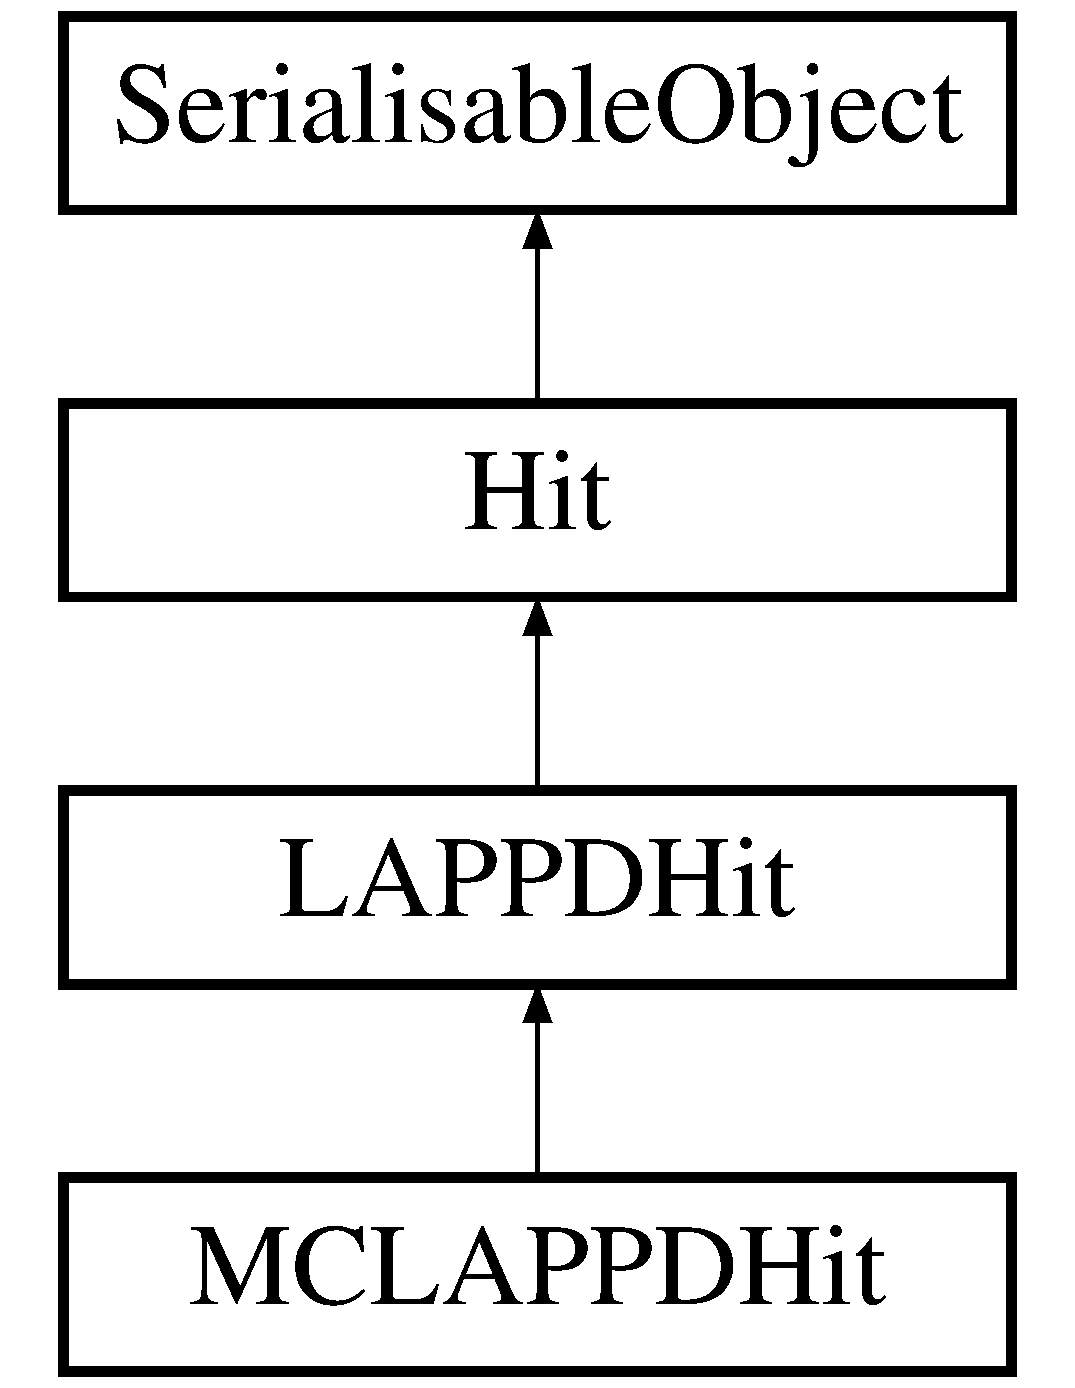
\includegraphics[height=4cm]{classLAPPDHit}
\end{center}
\end{figure}
\subsection*{Public Member Functions}
\begin{DoxyCompactItemize}
\item 
\hypertarget{classLAPPDHit_afe5f8ccfdc8ea9c3cbf1ceb9c441e71d}{
{\bfseries LAPPDHit} (int thetubeid, double thetime, double thecharge, std::vector$<$ double $>$ theposition, std::vector$<$ double $>$ thelocalposition)}
\label{classLAPPDHit_afe5f8ccfdc8ea9c3cbf1ceb9c441e71d}

\item 
\hypertarget{classLAPPDHit_ae1828d2ea7a97bc4fea858aaf94cedb4}{
std::vector$<$ double $>$ {\bfseries GetPosition} () const }
\label{classLAPPDHit_ae1828d2ea7a97bc4fea858aaf94cedb4}

\item 
\hypertarget{classLAPPDHit_a9d1c4249ca261677004dbb0ea65effb1}{
std::vector$<$ double $>$ {\bfseries GetLocalPosition} () const }
\label{classLAPPDHit_a9d1c4249ca261677004dbb0ea65effb1}

\item 
\hypertarget{classLAPPDHit_acddccb2ec31fd46be236b32ede3a783b}{
void {\bfseries SetPosition} (std::vector$<$ double $>$ pos)}
\label{classLAPPDHit_acddccb2ec31fd46be236b32ede3a783b}

\item 
\hypertarget{classLAPPDHit_a21e01043d24da9974933bbcfa2d23d3c}{
void {\bfseries SetLocalPosition} (std::vector$<$ double $>$ locpos)}
\label{classLAPPDHit_a21e01043d24da9974933bbcfa2d23d3c}

\item 
\hypertarget{classLAPPDHit_af993f8cd1441e7a37e8e1ca0e6890654}{
bool {\bfseries Print} ()}
\label{classLAPPDHit_af993f8cd1441e7a37e8e1ca0e6890654}

\end{DoxyCompactItemize}
\subsection*{Protected Member Functions}
\begin{DoxyCompactItemize}
\item 
\hypertarget{classLAPPDHit_a3039a8854f0295a7e517c159277bfa3f}{
{\footnotesize template$<$class Archive $>$ }\\void {\bfseries serialize} (Archive \&ar, const unsigned int version)}
\label{classLAPPDHit_a3039a8854f0295a7e517c159277bfa3f}

\end{DoxyCompactItemize}
\subsection*{Protected Attributes}
\begin{DoxyCompactItemize}
\item 
\hypertarget{classLAPPDHit_a979fc1e4b88cb77cac43c4dc3582ce3d}{
std::vector$<$ double $>$ {\bfseries Position}}
\label{classLAPPDHit_a979fc1e4b88cb77cac43c4dc3582ce3d}

\item 
\hypertarget{classLAPPDHit_a5517affe4e65ca692ce67160cd361d85}{
std::vector$<$ double $>$ {\bfseries LocalPosition}}
\label{classLAPPDHit_a5517affe4e65ca692ce67160cd361d85}

\end{DoxyCompactItemize}
\subsection*{Friends}
\begin{DoxyCompactItemize}
\item 
\hypertarget{classLAPPDHit_ac98d07dd8f7b70e16ccb9a01abf56b9c}{
class {\bfseries boost::serialization::access}}
\label{classLAPPDHit_ac98d07dd8f7b70e16ccb9a01abf56b9c}

\end{DoxyCompactItemize}


The documentation for this class was generated from the following file:\begin{DoxyCompactItemize}
\item 
DataModel/LAPPDHit.h\end{DoxyCompactItemize}

\hypertarget{classLAPPDIntegratePulse}{
\section{LAPPDIntegratePulse Class Reference}
\label{classLAPPDIntegratePulse}\index{LAPPDIntegratePulse@{LAPPDIntegratePulse}}
}
\subsection*{Public Member Functions}
\begin{DoxyCompactItemize}
\item 
\hypertarget{classLAPPDIntegratePulse_ab68036bfa8f3ae98552907590df7d57a}{
bool {\bfseries Initialise} (std::string configfile, \hyperlink{classDataModel}{DataModel} \&data)}
\label{classLAPPDIntegratePulse_ab68036bfa8f3ae98552907590df7d57a}

\item 
\hypertarget{classLAPPDIntegratePulse_ada15e2fbf5c978255a848d0e8dce064a}{
bool {\bfseries Execute} ()}
\label{classLAPPDIntegratePulse_ada15e2fbf5c978255a848d0e8dce064a}

\item 
\hypertarget{classLAPPDIntegratePulse_ab17c0fe3193abd1970c6148049bacc18}{
bool {\bfseries Finalise} ()}
\label{classLAPPDIntegratePulse_ab17c0fe3193abd1970c6148049bacc18}

\end{DoxyCompactItemize}


The documentation for this class was generated from the following files:\begin{DoxyCompactItemize}
\item 
UserTools/LAPPDIntegratePulse/LAPPDIntegratePulse.h\item 
UserTools/LAPPDIntegratePulse/LAPPDIntegratePulse.cpp\end{DoxyCompactItemize}

\hypertarget{classLAPPDlasertestHitFinder}{\section{L\-A\-P\-P\-Dlasertest\-Hit\-Finder Class Reference}
\label{classLAPPDlasertestHitFinder}\index{L\-A\-P\-P\-Dlasertest\-Hit\-Finder@{L\-A\-P\-P\-Dlasertest\-Hit\-Finder}}
}
Inheritance diagram for L\-A\-P\-P\-Dlasertest\-Hit\-Finder\-:\begin{figure}[H]
\begin{center}
\leavevmode
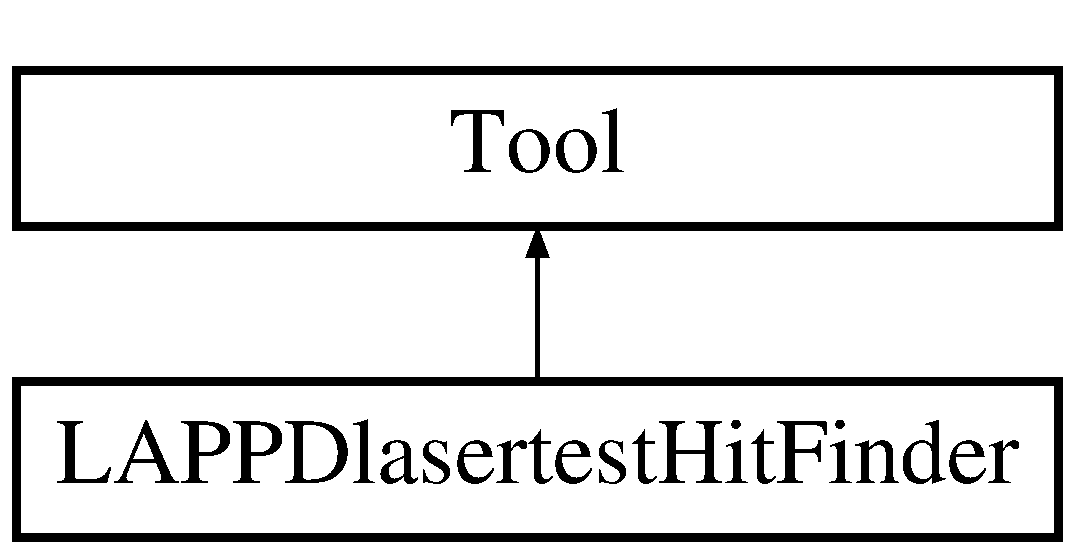
\includegraphics[height=2.000000cm]{classLAPPDlasertestHitFinder}
\end{center}
\end{figure}
\subsection*{Public Member Functions}
\begin{DoxyCompactItemize}
\item 
\hypertarget{classLAPPDlasertestHitFinder_a0a4dd1a750223833c9eb520008d4f821}{bool {\bfseries Initialise} (std\-::string configfile, \hyperlink{classDataModel}{Data\-Model} \&data)}\label{classLAPPDlasertestHitFinder_a0a4dd1a750223833c9eb520008d4f821}

\item 
\hypertarget{classLAPPDlasertestHitFinder_a028ed1741a9dd6048638a8e6f95f718a}{bool {\bfseries Execute} ()}\label{classLAPPDlasertestHitFinder_a028ed1741a9dd6048638a8e6f95f718a}

\item 
\hypertarget{classLAPPDlasertestHitFinder_a0ca3d1db237531ab1954a79f4ae469bd}{bool {\bfseries Finalise} ()}\label{classLAPPDlasertestHitFinder_a0ca3d1db237531ab1954a79f4ae469bd}

\end{DoxyCompactItemize}


The documentation for this class was generated from the following files\-:\begin{DoxyCompactItemize}
\item 
User\-Tools/\-L\-A\-P\-P\-Dlasertest\-Hit\-Finder/L\-A\-P\-P\-Dlasertest\-Hit\-Finder.\-h\item 
User\-Tools/\-L\-A\-P\-P\-Dlasertest\-Hit\-Finder/L\-A\-P\-P\-Dlasertest\-Hit\-Finder.\-cpp\end{DoxyCompactItemize}

\hypertarget{classLAPPDParseACC}{\section{L\-A\-P\-P\-D\-Parse\-A\-C\-C Class Reference}
\label{classLAPPDParseACC}\index{L\-A\-P\-P\-D\-Parse\-A\-C\-C@{L\-A\-P\-P\-D\-Parse\-A\-C\-C}}
}
Inheritance diagram for L\-A\-P\-P\-D\-Parse\-A\-C\-C\-:\begin{figure}[H]
\begin{center}
\leavevmode
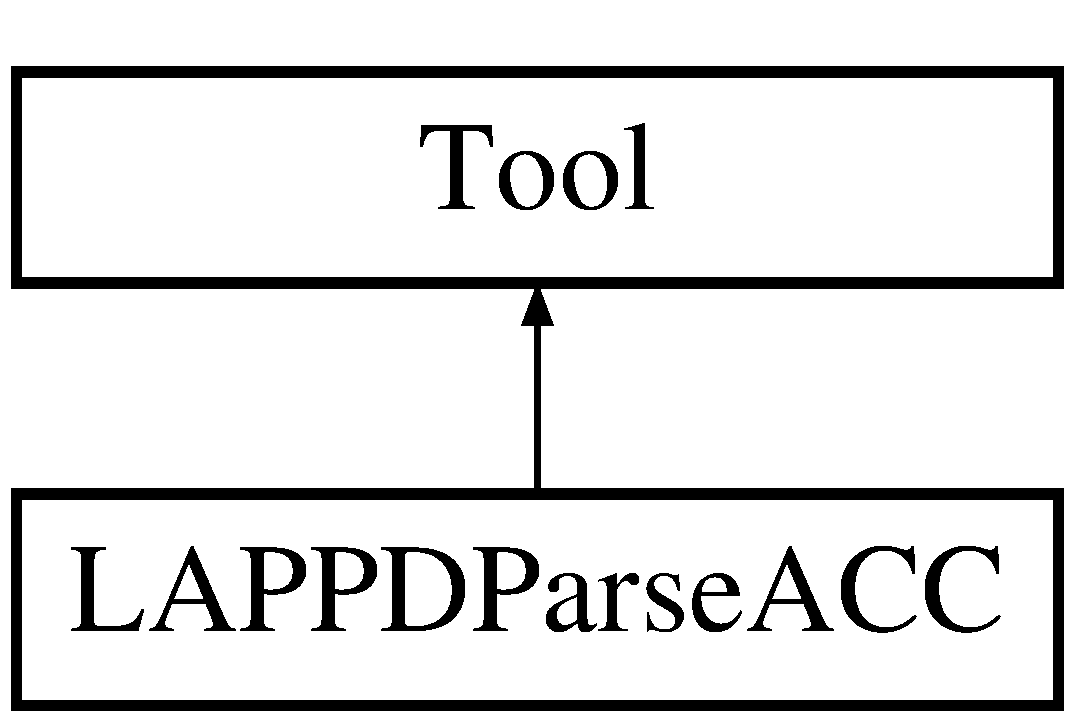
\includegraphics[height=2.000000cm]{classLAPPDParseACC}
\end{center}
\end{figure}
\subsection*{Public Member Functions}
\begin{DoxyCompactItemize}
\item 
\hypertarget{classLAPPDParseACC_acb7a9ca57ebef424c67ee6b2452c865e}{bool {\bfseries Initialise} (std\-::string configfile, \hyperlink{classDataModel}{Data\-Model} \&data)}\label{classLAPPDParseACC_acb7a9ca57ebef424c67ee6b2452c865e}

\item 
\hypertarget{classLAPPDParseACC_a398f4910f5179cc7463302c52a7280fb}{bool {\bfseries Execute} ()}\label{classLAPPDParseACC_a398f4910f5179cc7463302c52a7280fb}

\item 
\hypertarget{classLAPPDParseACC_a27d71df3f3481f978a819ea1830367ae}{bool {\bfseries Finalise} ()}\label{classLAPPDParseACC_a27d71df3f3481f978a819ea1830367ae}

\end{DoxyCompactItemize}


The documentation for this class was generated from the following files\-:\begin{DoxyCompactItemize}
\item 
User\-Tools/\-L\-A\-P\-P\-D\-Parse\-A\-C\-C/L\-A\-P\-P\-D\-Parse\-A\-C\-C.\-h\item 
User\-Tools/\-L\-A\-P\-P\-D\-Parse\-A\-C\-C/L\-A\-P\-P\-D\-Parse\-A\-C\-C.\-cpp\end{DoxyCompactItemize}

\hypertarget{classLAPPDParseScope}{
\section{LAPPDParseScope Class Reference}
\label{classLAPPDParseScope}\index{LAPPDParseScope@{LAPPDParseScope}}
}
\subsection*{Public Member Functions}
\begin{DoxyCompactItemize}
\item 
\hypertarget{classLAPPDParseScope_a5b2511aa79384f73240784028b39d427}{
bool {\bfseries Initialise} (std::string configfile, \hyperlink{classDataModel}{DataModel} \&data)}
\label{classLAPPDParseScope_a5b2511aa79384f73240784028b39d427}

\item 
\hypertarget{classLAPPDParseScope_ade2b40ff4ad384ab3778cb991bde62b6}{
bool {\bfseries Execute} ()}
\label{classLAPPDParseScope_ade2b40ff4ad384ab3778cb991bde62b6}

\item 
\hypertarget{classLAPPDParseScope_a7582fc226353ddceea5a73ff48d8c6a1}{
bool {\bfseries Finalise} ()}
\label{classLAPPDParseScope_a7582fc226353ddceea5a73ff48d8c6a1}

\end{DoxyCompactItemize}


The documentation for this class was generated from the following files:\begin{DoxyCompactItemize}
\item 
UserTools/LAPPDParseScope/LAPPDParseScope.h\item 
UserTools/LAPPDParseScope/LAPPDParseScope.cpp\end{DoxyCompactItemize}

\hypertarget{classLAPPDPulse}{\section{L\-A\-P\-P\-D\-Pulse Class Reference}
\label{classLAPPDPulse}\index{L\-A\-P\-P\-D\-Pulse@{L\-A\-P\-P\-D\-Pulse}}
}
Inheritance diagram for L\-A\-P\-P\-D\-Pulse\-:\begin{figure}[H]
\begin{center}
\leavevmode
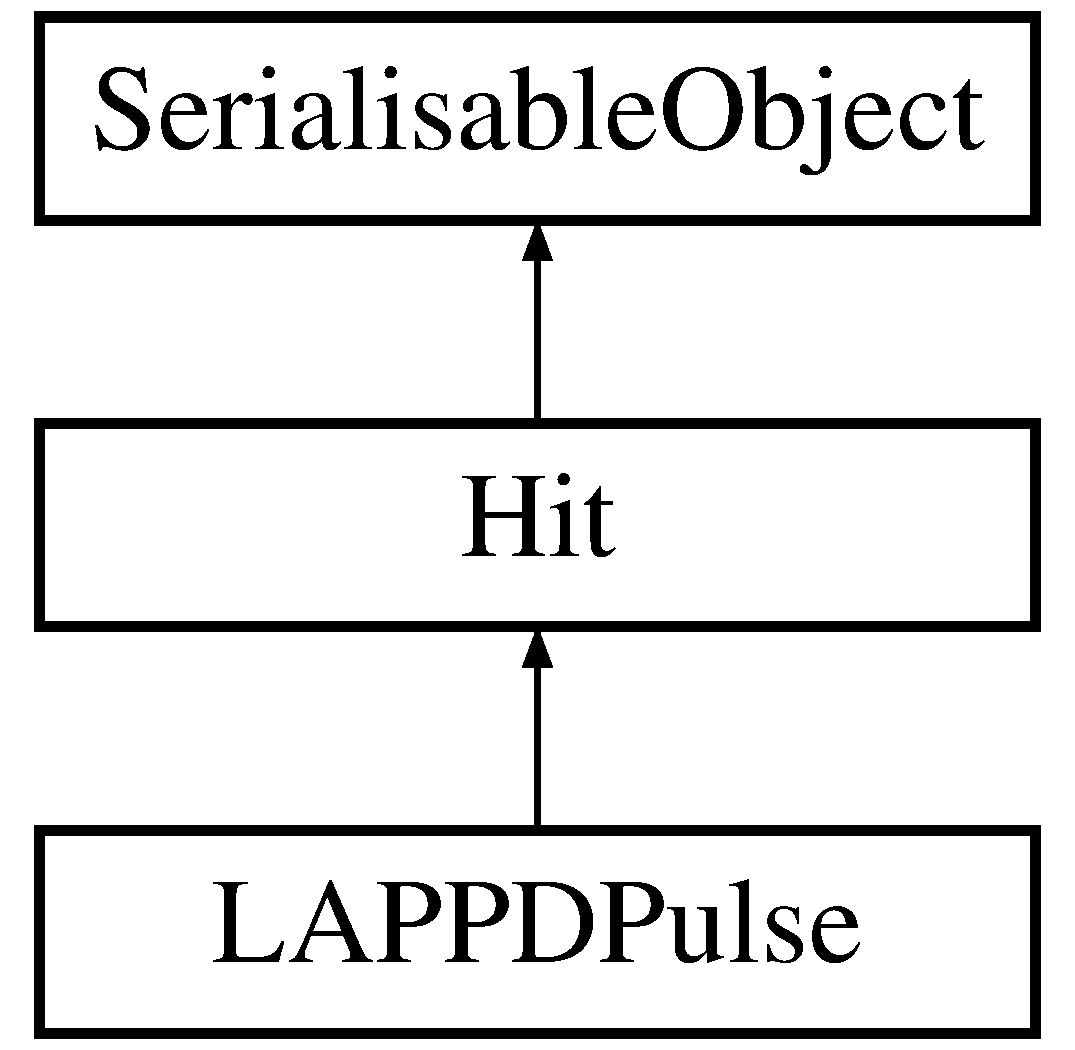
\includegraphics[height=3.000000cm]{classLAPPDPulse}
\end{center}
\end{figure}
\subsection*{Public Member Functions}
\begin{DoxyCompactItemize}
\item 
\hypertarget{classLAPPDPulse_ab6d60a683e420fd6304cc8d06b56e3f6}{{\bfseries L\-A\-P\-P\-D\-Pulse} (int tubeid, int channelid, double thetime, double charge, double peak, double low, double hi)}\label{classLAPPDPulse_ab6d60a683e420fd6304cc8d06b56e3f6}

\item 
\hypertarget{classLAPPDPulse_af0a8fed16c7b5c00f8bb644fb5b5a862}{int {\bfseries Get\-Channel\-I\-D} ()}\label{classLAPPDPulse_af0a8fed16c7b5c00f8bb644fb5b5a862}

\item 
\hypertarget{classLAPPDPulse_a86ef7d81b63accf60eea72dffd3c578d}{double {\bfseries Get\-Peak} ()}\label{classLAPPDPulse_a86ef7d81b63accf60eea72dffd3c578d}

\item 
\hypertarget{classLAPPDPulse_ac60601aee23092e71c13b953415d9d6d}{double {\bfseries Get\-Low\-Range} ()}\label{classLAPPDPulse_ac60601aee23092e71c13b953415d9d6d}

\item 
\hypertarget{classLAPPDPulse_a471f03a01ed49ef0db9438d13fe12200}{double {\bfseries Get\-Hi\-Range} ()}\label{classLAPPDPulse_a471f03a01ed49ef0db9438d13fe12200}

\item 
\hypertarget{classLAPPDPulse_ae3dad03fc206ae35ad7799ffe892f949}{void {\bfseries Set\-Channel\-I\-D} (int channelid)}\label{classLAPPDPulse_ae3dad03fc206ae35ad7799ffe892f949}

\item 
\hypertarget{classLAPPDPulse_a0c08b4bd1739552c7d6e2ad8cd9541e5}{void {\bfseries Set\-Peak} (double peak)}\label{classLAPPDPulse_a0c08b4bd1739552c7d6e2ad8cd9541e5}

\item 
\hypertarget{classLAPPDPulse_ae9345baa2efd05784e2b5c3c7023c194}{void {\bfseries Set\-Range} (double low, double hi)}\label{classLAPPDPulse_ae9345baa2efd05784e2b5c3c7023c194}

\item 
\hypertarget{classLAPPDPulse_a96fde20895fdcf61eb055308ed0b962d}{bool {\bfseries Print} ()}\label{classLAPPDPulse_a96fde20895fdcf61eb055308ed0b962d}

\end{DoxyCompactItemize}
\subsection*{Protected Member Functions}
\begin{DoxyCompactItemize}
\item 
\hypertarget{classLAPPDPulse_aa51fb4050ecce1aca2beb008a272d766}{{\footnotesize template$<$class Archive $>$ }\\void {\bfseries serialize} (Archive \&ar, const unsigned int version)}\label{classLAPPDPulse_aa51fb4050ecce1aca2beb008a272d766}

\end{DoxyCompactItemize}
\subsection*{Protected Attributes}
\begin{DoxyCompactItemize}
\item 
\hypertarget{classLAPPDPulse_a2e42975bd2fd735b7bd7d7c2bacb683f}{double {\bfseries Channel\-I\-D}}\label{classLAPPDPulse_a2e42975bd2fd735b7bd7d7c2bacb683f}

\item 
\hypertarget{classLAPPDPulse_a72893cf5f3accbe429e2cb1437b02064}{double {\bfseries Peak}}\label{classLAPPDPulse_a72893cf5f3accbe429e2cb1437b02064}

\item 
\hypertarget{classLAPPDPulse_af4923695ff523930e7109fab7743d7c4}{double {\bfseries Low\-Range}}\label{classLAPPDPulse_af4923695ff523930e7109fab7743d7c4}

\item 
\hypertarget{classLAPPDPulse_a5ee5c47716e498114b8924a64a92b562}{double {\bfseries Hi\-Range}}\label{classLAPPDPulse_a5ee5c47716e498114b8924a64a92b562}

\end{DoxyCompactItemize}
\subsection*{Friends}
\begin{DoxyCompactItemize}
\item 
\hypertarget{classLAPPDPulse_ac98d07dd8f7b70e16ccb9a01abf56b9c}{class {\bfseries boost\-::serialization\-::access}}\label{classLAPPDPulse_ac98d07dd8f7b70e16ccb9a01abf56b9c}

\end{DoxyCompactItemize}


The documentation for this class was generated from the following file\-:\begin{DoxyCompactItemize}
\item 
Data\-Model/L\-A\-P\-P\-D\-Pulse.\-h\end{DoxyCompactItemize}

\hypertarget{classLAPPDresponse}{\section{L\-A\-P\-P\-Dresponse Class Reference}
\label{classLAPPDresponse}\index{L\-A\-P\-P\-Dresponse@{L\-A\-P\-P\-Dresponse}}
}
\subsection*{Public Member Functions}
\begin{DoxyCompactItemize}
\item 
\hypertarget{classLAPPDresponse_a5d53c8ca94cd0b1d2f389df41b3c71d0}{void {\bfseries Add\-Single\-Photon\-Trace} (double trans, double para, double time)}\label{classLAPPDresponse_a5d53c8ca94cd0b1d2f389df41b3c71d0}

\item 
\hypertarget{classLAPPDresponse_a6dc34922a8a63dc84fa2758ad7ae07f5}{\hyperlink{classWaveform}{Waveform}$<$ double $>$ {\bfseries Get\-Trace} (int C\-Hnumber, double starttime, double samplesize, int numsamples, double thenoise)}\label{classLAPPDresponse_a6dc34922a8a63dc84fa2758ad7ae07f5}

\item 
\hypertarget{classLAPPDresponse_af7ea4eaf42b67cd816a1205c84e9756b}{int {\bfseries Find\-Strip\-Number} (double trans)}\label{classLAPPDresponse_af7ea4eaf42b67cd816a1205c84e9756b}

\item 
\hypertarget{classLAPPDresponse_a7006a41063a44bec116b5763dfd218ac}{double {\bfseries Strip\-Coordinate} (int stripnumber)}\label{classLAPPDresponse_a7006a41063a44bec116b5763dfd218ac}

\item 
\hypertarget{classLAPPDresponse_a5d53c8ca94cd0b1d2f389df41b3c71d0}{void {\bfseries Add\-Single\-Photon\-Trace} (double trans, double para, double time)}\label{classLAPPDresponse_a5d53c8ca94cd0b1d2f389df41b3c71d0}

\item 
\hypertarget{classLAPPDresponse_adcf4b1cb461f805e4f2b0106ad24a87d}{\hyperlink{classWaveform}{Waveform}$<$ double $>$ {\bfseries Get\-Trace} (int C\-Hnumber, double starttime, double samplesize, int numsamples, double thenoise)}\label{classLAPPDresponse_adcf4b1cb461f805e4f2b0106ad24a87d}

\item 
\hypertarget{classLAPPDresponse_af7ea4eaf42b67cd816a1205c84e9756b}{int {\bfseries Find\-Strip\-Number} (double trans)}\label{classLAPPDresponse_af7ea4eaf42b67cd816a1205c84e9756b}

\item 
\hypertarget{classLAPPDresponse_a7006a41063a44bec116b5763dfd218ac}{double {\bfseries Strip\-Coordinate} (int stripnumber)}\label{classLAPPDresponse_a7006a41063a44bec116b5763dfd218ac}

\end{DoxyCompactItemize}
\subsection*{Public Attributes}
\begin{DoxyCompactItemize}
\item 
\hypertarget{classLAPPDresponse_ae10b5dcda1903b993df6891d60b1e0d4}{map$<$ int, vector$<$ \hyperlink{classLAPPDPulse}{L\-A\-P\-P\-D\-Pulse} $>$ $>$ {\bfseries L\-A\-P\-P\-D\-Pulse\-Cluster}}\label{classLAPPDresponse_ae10b5dcda1903b993df6891d60b1e0d4}

\end{DoxyCompactItemize}


The documentation for this class was generated from the following files\-:\begin{DoxyCompactItemize}
\item 
User\-Tools/\-Histograms\-Root\-L\-A\-P\-P\-D\-Data/L\-A\-P\-P\-Dresponse.\-hh\item 
User\-Tools/\-L\-A\-P\-P\-D\-Sim/L\-A\-P\-P\-Dresponse.\-hh\item 
User\-Tools/\-L\-A\-P\-P\-D\-Sim/L\-A\-P\-P\-Dresponse.\-cpp\end{DoxyCompactItemize}

\hypertarget{classLAPPDSaveROOT}{\section{L\-A\-P\-P\-D\-Save\-R\-O\-O\-T Class Reference}
\label{classLAPPDSaveROOT}\index{L\-A\-P\-P\-D\-Save\-R\-O\-O\-T@{L\-A\-P\-P\-D\-Save\-R\-O\-O\-T}}
}
Inheritance diagram for L\-A\-P\-P\-D\-Save\-R\-O\-O\-T\-:\begin{figure}[H]
\begin{center}
\leavevmode
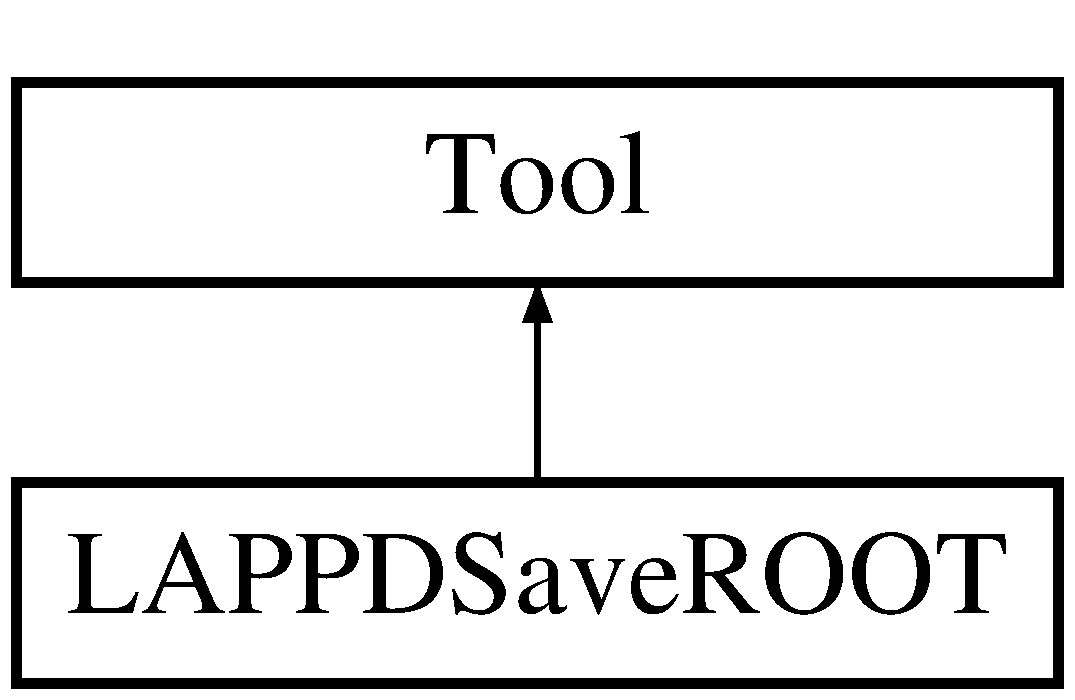
\includegraphics[height=2.000000cm]{classLAPPDSaveROOT}
\end{center}
\end{figure}
\subsection*{Public Member Functions}
\begin{DoxyCompactItemize}
\item 
\hypertarget{classLAPPDSaveROOT_aca0e74a9dacc21f8d0b6f19925bb610f}{bool {\bfseries Initialise} (std\-::string configfile, \hyperlink{classDataModel}{Data\-Model} \&data)}\label{classLAPPDSaveROOT_aca0e74a9dacc21f8d0b6f19925bb610f}

\item 
\hypertarget{classLAPPDSaveROOT_ae88cb83e263fc39a17b3a1b376b713d8}{bool {\bfseries Execute} ()}\label{classLAPPDSaveROOT_ae88cb83e263fc39a17b3a1b376b713d8}

\item 
\hypertarget{classLAPPDSaveROOT_a9e91575ae339177f32be29eaefd963af}{bool {\bfseries Finalise} ()}\label{classLAPPDSaveROOT_a9e91575ae339177f32be29eaefd963af}

\end{DoxyCompactItemize}


The documentation for this class was generated from the following files\-:\begin{DoxyCompactItemize}
\item 
User\-Tools/\-L\-A\-P\-P\-D\-Save\-R\-O\-O\-T/L\-A\-P\-P\-D\-Save\-R\-O\-O\-T.\-h\item 
User\-Tools/\-L\-A\-P\-P\-D\-Save\-R\-O\-O\-T/L\-A\-P\-P\-D\-Save\-R\-O\-O\-T.\-cpp\end{DoxyCompactItemize}

\hypertarget{classLAPPDSim}{
\section{LAPPDSim Class Reference}
\label{classLAPPDSim}\index{LAPPDSim@{LAPPDSim}}
}
\subsection*{Public Member Functions}
\begin{DoxyCompactItemize}
\item 
\hypertarget{classLAPPDSim_a68edcbace6d4b83bff31e3866d0cbfc1}{
bool {\bfseries Initialise} (std::string configfile, \hyperlink{classDataModel}{DataModel} \&data)}
\label{classLAPPDSim_a68edcbace6d4b83bff31e3866d0cbfc1}

\item 
\hypertarget{classLAPPDSim_a0d34e153938d2a1c6fab9c3083862000}{
bool {\bfseries Execute} ()}
\label{classLAPPDSim_a0d34e153938d2a1c6fab9c3083862000}

\item 
\hypertarget{classLAPPDSim_a97d903656a7ddbdafb5170bb672193ba}{
bool {\bfseries Finalise} ()}
\label{classLAPPDSim_a97d903656a7ddbdafb5170bb672193ba}

\item 
\hypertarget{classLAPPDSim_ab08ad145a8cea2e3d0283ba48b91fa47}{
\hyperlink{classWaveform}{Waveform}$<$ double $>$ {\bfseries SimpleGenPulse} (vector$<$ double $>$ pulsetimes)}
\label{classLAPPDSim_ab08ad145a8cea2e3d0283ba48b91fa47}

\end{DoxyCompactItemize}


The documentation for this class was generated from the following files:\begin{DoxyCompactItemize}
\item 
UserTools/LAPPDSim/LAPPDSim.h\item 
UserTools/LAPPDSim/LAPPDSim.cpp\end{DoxyCompactItemize}

\hypertarget{classLAPPDTree}{
\section{LAPPDTree Class Reference}
\label{classLAPPDTree}\index{LAPPDTree@{LAPPDTree}}
}
\subsection*{Public Member Functions}
\begin{DoxyCompactItemize}
\item 
\hypertarget{classLAPPDTree_abb24c0d515c12bc1809d5d0bf7c6abc6}{
{\bfseries LAPPDTree} (TTree $\ast$tree=0)}
\label{classLAPPDTree_abb24c0d515c12bc1809d5d0bf7c6abc6}

\item 
\hypertarget{classLAPPDTree_a64600503669b4b3d36763db323ef56f3}{
{\bfseries LAPPDTree} (const char $\ast$filepath, bool addsubdirs=false)}
\label{classLAPPDTree_a64600503669b4b3d36763db323ef56f3}

\item 
\hypertarget{classLAPPDTree_a88072a0e2cc4fcceaa929968f3da46e3}{
virtual Int\_\-t {\bfseries Cut} (Long64\_\-t entry)}
\label{classLAPPDTree_a88072a0e2cc4fcceaa929968f3da46e3}

\item 
\hypertarget{classLAPPDTree_a1d8e6cc2426b400555882ee7851480c9}{
virtual Int\_\-t {\bfseries GetEntry} (Long64\_\-t entry)}
\label{classLAPPDTree_a1d8e6cc2426b400555882ee7851480c9}

\item 
\hypertarget{classLAPPDTree_a97dbcea6a6dae6197cdc672ce74867c0}{
virtual Long64\_\-t {\bfseries LoadTree} (Long64\_\-t entry)}
\label{classLAPPDTree_a97dbcea6a6dae6197cdc672ce74867c0}

\item 
\hypertarget{classLAPPDTree_a427214efe50a475c58e9287674be1f07}{
virtual void {\bfseries Init} (TTree $\ast$tree)}
\label{classLAPPDTree_a427214efe50a475c58e9287674be1f07}

\item 
\hypertarget{classLAPPDTree_ad16b2af53b7d2ab9a2f63514cd0de6b4}{
virtual void {\bfseries Loop} ()}
\label{classLAPPDTree_ad16b2af53b7d2ab9a2f63514cd0de6b4}

\item 
\hypertarget{classLAPPDTree_aa811db4c6d3e7c433eb38f2f4769d817}{
virtual Bool\_\-t {\bfseries Notify} ()}
\label{classLAPPDTree_aa811db4c6d3e7c433eb38f2f4769d817}

\item 
\hypertarget{classLAPPDTree_ac5221c09835edce1fa0ad0858c045e82}{
virtual void {\bfseries Show} (Long64\_\-t entry=-\/1)}
\label{classLAPPDTree_ac5221c09835edce1fa0ad0858c045e82}

\item 
\hypertarget{classLAPPDTree_a5e16fe0d23c4821887fd356eb48b95a5}{
TChain $\ast$ {\bfseries AddFiles} (const char $\ast$inputdir, bool addsubfolders)}
\label{classLAPPDTree_a5e16fe0d23c4821887fd356eb48b95a5}

\end{DoxyCompactItemize}
\subsection*{Public Attributes}
\begin{DoxyCompactItemize}
\item 
\hypertarget{classLAPPDTree_ab7334c305d8c67c1469b286cd775845c}{
TTree $\ast$ {\bfseries fChain}}
\label{classLAPPDTree_ab7334c305d8c67c1469b286cd775845c}

\item 
\hypertarget{classLAPPDTree_a57ea0164e27a936105e60d5a7910335d}{
Int\_\-t \hyperlink{classLAPPDTree_a57ea0164e27a936105e60d5a7910335d}{fCurrent}}
\label{classLAPPDTree_a57ea0164e27a936105e60d5a7910335d}

\begin{DoxyCompactList}\small\item\em pointer to the analyzed TTree or TChain \item\end{DoxyCompactList}\item 
\hypertarget{classLAPPDTree_af6c1ba92cb9a0f70418af64563f7bccf}{
int \hyperlink{classLAPPDTree_af6c1ba92cb9a0f70418af64563f7bccf}{verbose} = 1}
\label{classLAPPDTree_af6c1ba92cb9a0f70418af64563f7bccf}

\begin{DoxyCompactList}\small\item\em current Tree number in a TChain \item\end{DoxyCompactList}\item 
\hypertarget{classLAPPDTree_a3a198c1cfd76e782b371ae2eddc911d7}{
Int\_\-t {\bfseries lappdevt}}
\label{classLAPPDTree_a3a198c1cfd76e782b371ae2eddc911d7}

\item 
\hypertarget{classLAPPDTree_a82b4e313a76045692cad281c966955b8}{
Int\_\-t {\bfseries lappd\_\-numhits}}
\label{classLAPPDTree_a82b4e313a76045692cad281c966955b8}

\item 
\hypertarget{classLAPPDTree_a92a142c36821ddf3a0dc240d57ace54f}{
Int\_\-t {\bfseries lappdhit\_\-objnum} \mbox{[}180\mbox{]}}
\label{classLAPPDTree_a92a142c36821ddf3a0dc240d57ace54f}

\item 
\hypertarget{classLAPPDTree_a7dbf3acc22501e676eac167d1c8bfb91}{
Double\_\-t {\bfseries lappdhit\_\-x} \mbox{[}180\mbox{]}}
\label{classLAPPDTree_a7dbf3acc22501e676eac167d1c8bfb91}

\item 
\hypertarget{classLAPPDTree_a2bc97b493024b71430528a71c2339ec7}{
Double\_\-t {\bfseries lappdhit\_\-y} \mbox{[}180\mbox{]}}
\label{classLAPPDTree_a2bc97b493024b71430528a71c2339ec7}

\item 
\hypertarget{classLAPPDTree_a73e138836f63b843c99fbe3951f7e504}{
Double\_\-t {\bfseries lappdhit\_\-z} \mbox{[}180\mbox{]}}
\label{classLAPPDTree_a73e138836f63b843c99fbe3951f7e504}

\item 
\hypertarget{classLAPPDTree_aa5f1d299a73e165905b798a925206de5}{
vector$<$ double $>$ $\ast$ {\bfseries lappdhit\_\-stripcoorx}}
\label{classLAPPDTree_aa5f1d299a73e165905b798a925206de5}

\item 
\hypertarget{classLAPPDTree_a1a9420e83fa6ac964448bd89fb613248}{
vector$<$ double $>$ $\ast$ {\bfseries lappdhit\_\-stripcoory}}
\label{classLAPPDTree_a1a9420e83fa6ac964448bd89fb613248}

\item 
\hypertarget{classLAPPDTree_a07b7a60f594d559022c75cc8962a673e}{
vector$<$ double $>$ $\ast$ {\bfseries lappdhit\_\-stripcoort}}
\label{classLAPPDTree_a07b7a60f594d559022c75cc8962a673e}

\item 
\hypertarget{classLAPPDTree_a361c88caa35c7b75c6625d1726fd3116}{
Double\_\-t {\bfseries lappdhit\_\-edep} \mbox{[}180\mbox{]}}
\label{classLAPPDTree_a361c88caa35c7b75c6625d1726fd3116}

\item 
\hypertarget{classLAPPDTree_abbf80a1da763ec467ead614fd4289718}{
vector$<$ double $>$ $\ast$ {\bfseries lappdhit\_\-globalcoorx}}
\label{classLAPPDTree_abbf80a1da763ec467ead614fd4289718}

\item 
\hypertarget{classLAPPDTree_a4d4353d05db2632541d8a34b825cc5e8}{
vector$<$ double $>$ $\ast$ {\bfseries lappdhit\_\-globalcoory}}
\label{classLAPPDTree_a4d4353d05db2632541d8a34b825cc5e8}

\item 
\hypertarget{classLAPPDTree_a44dc4554d5ea50fe0043d6d5e83292d4}{
vector$<$ double $>$ $\ast$ {\bfseries lappdhit\_\-globalcoorz}}
\label{classLAPPDTree_a44dc4554d5ea50fe0043d6d5e83292d4}

\item 
\hypertarget{classLAPPDTree_a842bd00c916ff704c337885e944a2597}{
vector$<$ double $>$ {\bfseries lappdhit\_\-globalcoorxdummy}}
\label{classLAPPDTree_a842bd00c916ff704c337885e944a2597}

\item 
\hypertarget{classLAPPDTree_a43f80af2bdabd39c31346a526b8e9a5c}{
vector$<$ double $>$ {\bfseries lappdhit\_\-globalcoorydummy}}
\label{classLAPPDTree_a43f80af2bdabd39c31346a526b8e9a5c}

\item 
\hypertarget{classLAPPDTree_a9ed8c2c3aa42ecc9fbaa575caa076940}{
vector$<$ double $>$ {\bfseries lappdhit\_\-globalcoorzdummy}}
\label{classLAPPDTree_a9ed8c2c3aa42ecc9fbaa575caa076940}

\item 
\hypertarget{classLAPPDTree_a372097f371b2bbd414b6447da2e5fd51}{
vector$<$ int $>$ $\ast$ {\bfseries lappdhit\_\-primaryParentID2}}
\label{classLAPPDTree_a372097f371b2bbd414b6447da2e5fd51}

\item 
\hypertarget{classLAPPDTree_af47a619c8a87743efecb91b7fbf2c7be}{
TBranch $\ast$ {\bfseries b\_\-lappdevt}}
\label{classLAPPDTree_af47a619c8a87743efecb91b7fbf2c7be}

\item 
\hypertarget{classLAPPDTree_af2d3bcf8ac6d1984ddd5da708841fd81}{
TBranch $\ast$ {\bfseries b\_\-lappd\_\-numhits}}
\label{classLAPPDTree_af2d3bcf8ac6d1984ddd5da708841fd81}

\item 
\hypertarget{classLAPPDTree_aaffff4e3fa3c778499625bc2c79179de}{
TBranch $\ast$ {\bfseries b\_\-lappdhit\_\-totalpes\_\-perevt}}
\label{classLAPPDTree_aaffff4e3fa3c778499625bc2c79179de}

\item 
\hypertarget{classLAPPDTree_a97ffd58d9a74db4d2026aea619e55c3e}{
TBranch $\ast$ {\bfseries b\_\-lappdhit\_\-totalpes\_\-perlappd2}}
\label{classLAPPDTree_a97ffd58d9a74db4d2026aea619e55c3e}

\item 
\hypertarget{classLAPPDTree_aaa3ff0b6eefee590df4209064eb2907f}{
TBranch $\ast$ {\bfseries b\_\-lappdhit\_\-x}}
\label{classLAPPDTree_aaa3ff0b6eefee590df4209064eb2907f}

\item 
\hypertarget{classLAPPDTree_adc45ffd7b8f116526d1683182a8b0104}{
TBranch $\ast$ {\bfseries b\_\-lappdhit\_\-y}}
\label{classLAPPDTree_adc45ffd7b8f116526d1683182a8b0104}

\item 
\hypertarget{classLAPPDTree_ac15eb6f5a771b3a8a4af9f98ef64642c}{
TBranch $\ast$ {\bfseries b\_\-lappdhit\_\-z}}
\label{classLAPPDTree_ac15eb6f5a771b3a8a4af9f98ef64642c}

\item 
\hypertarget{classLAPPDTree_a321a08fed926fdb6e506cf99e3036932}{
TBranch $\ast$ {\bfseries b\_\-lappdhit\_\-stripcoorx}}
\label{classLAPPDTree_a321a08fed926fdb6e506cf99e3036932}

\item 
\hypertarget{classLAPPDTree_a08b0df3f4c28158e497a5d54b4c52646}{
TBranch $\ast$ {\bfseries b\_\-lappdhit\_\-stripcoory}}
\label{classLAPPDTree_a08b0df3f4c28158e497a5d54b4c52646}

\item 
\hypertarget{classLAPPDTree_af7b4cf0126506fa7159848c569bd9a0b}{
TBranch $\ast$ {\bfseries b\_\-lappdhit\_\-stripcoorz}}
\label{classLAPPDTree_af7b4cf0126506fa7159848c569bd9a0b}

\item 
\hypertarget{classLAPPDTree_a825861f9f2cc7aae1554b316ef8d39a9}{
TBranch $\ast$ {\bfseries b\_\-lappdhit\_\-stripcoort}}
\label{classLAPPDTree_a825861f9f2cc7aae1554b316ef8d39a9}

\item 
\hypertarget{classLAPPDTree_a2f1588991d3a64b51f09aad302903044}{
TBranch $\ast$ {\bfseries b\_\-lappdhit\_\-globalcoorx}}
\label{classLAPPDTree_a2f1588991d3a64b51f09aad302903044}

\item 
\hypertarget{classLAPPDTree_a1f5965eb70d5028bae942cd81ebf6820}{
TBranch $\ast$ {\bfseries b\_\-lappdhit\_\-globalcoory}}
\label{classLAPPDTree_a1f5965eb70d5028bae942cd81ebf6820}

\item 
\hypertarget{classLAPPDTree_a023ec732a7f88e6daca5480adff51a29}{
TBranch $\ast$ {\bfseries b\_\-lappdhit\_\-globalcoorz}}
\label{classLAPPDTree_a023ec732a7f88e6daca5480adff51a29}

\item 
\hypertarget{classLAPPDTree_ab0e08ad50302af8e404f4e133a8e7357}{
TBranch $\ast$ {\bfseries b\_\-lappdhit\_\-process}}
\label{classLAPPDTree_ab0e08ad50302af8e404f4e133a8e7357}

\item 
\hypertarget{classLAPPDTree_aee5aea4ed12b28c5784e951ab9004e4b}{
TBranch $\ast$ {\bfseries b\_\-lappdhit\_\-particleID}}
\label{classLAPPDTree_aee5aea4ed12b28c5784e951ab9004e4b}

\item 
\hypertarget{classLAPPDTree_a4d9f69bbc84a59dd42763349fb5abfc5}{
TBranch $\ast$ {\bfseries b\_\-lappdhit\_\-trackID}}
\label{classLAPPDTree_a4d9f69bbc84a59dd42763349fb5abfc5}

\item 
\hypertarget{classLAPPDTree_aa1dde2f8ca08d72d9f6ef2614935909f}{
TBranch $\ast$ {\bfseries b\_\-lappdhit\_\-edep}}
\label{classLAPPDTree_aa1dde2f8ca08d72d9f6ef2614935909f}

\item 
\hypertarget{classLAPPDTree_a8f6eea3420011bb1a15307d4ab38c8fd}{
TBranch $\ast$ {\bfseries b\_\-lappdhit\_\-objnum}}
\label{classLAPPDTree_a8f6eea3420011bb1a15307d4ab38c8fd}

\item 
\hypertarget{classLAPPDTree_a719cbac920cf65ff67af978dfbac12d2}{
TBranch $\ast$ {\bfseries b\_\-lappdhit\_\-stripnum}}
\label{classLAPPDTree_a719cbac920cf65ff67af978dfbac12d2}

\item 
\hypertarget{classLAPPDTree_a3ba0a48b444731d20574179863c896a6}{
TBranch $\ast$ {\bfseries b\_\-lappdhit\_\-truetime2}}
\label{classLAPPDTree_a3ba0a48b444731d20574179863c896a6}

\item 
\hypertarget{classLAPPDTree_a18aee356c45455494e3168712bc31f81}{
TBranch $\ast$ {\bfseries b\_\-lappdhit\_\-smeartime2}}
\label{classLAPPDTree_a18aee356c45455494e3168712bc31f81}

\item 
\hypertarget{classLAPPDTree_a41a93215c8835469b83d7ba9b5910783}{
TBranch $\ast$ {\bfseries b\_\-lappdhit\_\-primaryParentID2}}
\label{classLAPPDTree_a41a93215c8835469b83d7ba9b5910783}

\item 
\hypertarget{classLAPPDTree_a325d2982f6d588f05a852ca75aa850f8}{
TBranch $\ast$ {\bfseries b\_\-lappdhit\_\-NoOfneighstripsHit}}
\label{classLAPPDTree_a325d2982f6d588f05a852ca75aa850f8}

\item 
\hypertarget{classLAPPDTree_a54214ff49a3743466717febd048e0d20}{
TBranch $\ast$ {\bfseries b\_\-lappdhit\_\-neighstripnum}}
\label{classLAPPDTree_a54214ff49a3743466717febd048e0d20}

\item 
\hypertarget{classLAPPDTree_aa7b113f55684fabe737895d860c8ec7e}{
TBranch $\ast$ {\bfseries b\_\-lappdhit\_\-neighstrippeak}}
\label{classLAPPDTree_aa7b113f55684fabe737895d860c8ec7e}

\item 
\hypertarget{classLAPPDTree_ab8c7888fd048b0d5b6d8c15634ee7919}{
TBranch $\ast$ {\bfseries b\_\-lappdhit\_\-neighstrip\_\-time}}
\label{classLAPPDTree_ab8c7888fd048b0d5b6d8c15634ee7919}

\item 
\hypertarget{classLAPPDTree_adbf2e61a53af0c4f535b64b90e942f27}{
TBranch $\ast$ {\bfseries b\_\-lappdhit\_\-neighstrip\_\-lefttime}}
\label{classLAPPDTree_adbf2e61a53af0c4f535b64b90e942f27}

\item 
\hypertarget{classLAPPDTree_ae3992ee3c8fb6400ae25486d15bba708}{
TBranch $\ast$ {\bfseries b\_\-lappdhit\_\-neighstrip\_\-righttime}}
\label{classLAPPDTree_ae3992ee3c8fb6400ae25486d15bba708}

\end{DoxyCompactItemize}


The documentation for this class was generated from the following files:\begin{DoxyCompactItemize}
\item 
UserTools/LoadWCSimLAPPD/LAPPDTree.h\item 
UserTools/LoadWCSimLAPPD/LAPPDTree.cpp\end{DoxyCompactItemize}

\hypertarget{classLikelihoodFitterCheck}{
\section{LikelihoodFitterCheck Class Reference}
\label{classLikelihoodFitterCheck}\index{LikelihoodFitterCheck@{LikelihoodFitterCheck}}
}
\subsection*{Public Member Functions}
\begin{DoxyCompactItemize}
\item 
\hypertarget{classLikelihoodFitterCheck_a796e1357c908ddb2d16dd06d11daf199}{
bool {\bfseries Initialise} (std::string configfile, \hyperlink{classDataModel}{DataModel} \&data)}
\label{classLikelihoodFitterCheck_a796e1357c908ddb2d16dd06d11daf199}

\item 
bool \hyperlink{classLikelihoodFitterCheck_a7df99c1fac639db633877aeadde27ca7}{Execute} ()
\item 
\hypertarget{classLikelihoodFitterCheck_a4c454e19b497d56f47cd0d34632d5174}{
bool {\bfseries Finalise} ()}
\label{classLikelihoodFitterCheck_a4c454e19b497d56f47cd0d34632d5174}

\end{DoxyCompactItemize}


\subsection{Member Function Documentation}
\hypertarget{classLikelihoodFitterCheck_a7df99c1fac639db633877aeadde27ca7}{
\index{LikelihoodFitterCheck@{LikelihoodFitterCheck}!Execute@{Execute}}
\index{Execute@{Execute}!LikelihoodFitterCheck@{LikelihoodFitterCheck}}
\subsubsection[{Execute}]{\setlength{\rightskip}{0pt plus 5cm}bool LikelihoodFitterCheck::Execute ()}}
\label{classLikelihoodFitterCheck_a7df99c1fac639db633877aeadde27ca7}


$>$ Get digits from \char`\"{}RecoEvent\char`\"{}

$>$ Get digits from \char`\"{}RecoEvent\char`\"{} 

The documentation for this class was generated from the following files:\begin{DoxyCompactItemize}
\item 
UserTools/LikelihoodFitterCheck/LikelihoodFitterCheck.h\item 
UserTools/LikelihoodFitterCheck/LikelihoodFitterCheck.cpp\end{DoxyCompactItemize}

\hypertarget{classLoadANNIEEvent}{
\section{LoadANNIEEvent Class Reference}
\label{classLoadANNIEEvent}\index{LoadANNIEEvent@{LoadANNIEEvent}}
}
\subsection*{Public Member Functions}
\begin{DoxyCompactItemize}
\item 
\hypertarget{classLoadANNIEEvent_a273ac2b597344b138ff0142fa24bff06}{
bool {\bfseries Initialise} (std::string configfile, \hyperlink{classDataModel}{DataModel} \&data)}
\label{classLoadANNIEEvent_a273ac2b597344b138ff0142fa24bff06}

\item 
\hypertarget{classLoadANNIEEvent_af2c0686e7625d6a8ab5ebd692e78b182}{
bool {\bfseries Execute} ()}
\label{classLoadANNIEEvent_af2c0686e7625d6a8ab5ebd692e78b182}

\item 
\hypertarget{classLoadANNIEEvent_afcee0c0da54733f0c3dadb8c8879f494}{
bool {\bfseries Finalise} ()}
\label{classLoadANNIEEvent_afcee0c0da54733f0c3dadb8c8879f494}

\end{DoxyCompactItemize}
\subsection*{Protected Attributes}
\begin{DoxyCompactItemize}
\item 
\hypertarget{classLoadANNIEEvent_a1c9892604bb47cb58be2e7b6214ac773}{
int \hyperlink{classLoadANNIEEvent_a1c9892604bb47cb58be2e7b6214ac773}{verbosity\_\-}}
\label{classLoadANNIEEvent_a1c9892604bb47cb58be2e7b6214ac773}

\begin{DoxyCompactList}\small\item\em Integer code that determines the level of logging to show in the output. \item\end{DoxyCompactList}\item 
\hypertarget{classLoadANNIEEvent_a5de84624994fa2f83892fa7ad192c954}{
std::vector$<$ std::string $>$ \hyperlink{classLoadANNIEEvent_a5de84624994fa2f83892fa7ad192c954}{input\_\-filenames\_\-}}
\label{classLoadANNIEEvent_a5de84624994fa2f83892fa7ad192c954}

\begin{DoxyCompactList}\small\item\em Vector of filenames for each of the input files. \item\end{DoxyCompactList}\item 
\hypertarget{classLoadANNIEEvent_a9037abdb3ca42bcb45da4f76eaa5497f}{
size\_\-t \hyperlink{classLoadANNIEEvent_a9037abdb3ca42bcb45da4f76eaa5497f}{current\_\-entry\_\-}}
\label{classLoadANNIEEvent_a9037abdb3ca42bcb45da4f76eaa5497f}

\begin{DoxyCompactList}\small\item\em The index of the current entry in the ANNIEEvent store. \item\end{DoxyCompactList}\item 
\hypertarget{classLoadANNIEEvent_a92adda94f9be56cfb8a6507aa64d16f6}{
size\_\-t \hyperlink{classLoadANNIEEvent_a92adda94f9be56cfb8a6507aa64d16f6}{current\_\-file\_\-}}
\label{classLoadANNIEEvent_a92adda94f9be56cfb8a6507aa64d16f6}

\begin{DoxyCompactList}\small\item\em The index of the current file in this list of input files. \item\end{DoxyCompactList}\item 
\hypertarget{classLoadANNIEEvent_aabbd70eb8db780eb690f58cf76b7178e}{
size\_\-t \hyperlink{classLoadANNIEEvent_aabbd70eb8db780eb690f58cf76b7178e}{total\_\-entries\_\-in\_\-file\_\-}}
\label{classLoadANNIEEvent_aabbd70eb8db780eb690f58cf76b7178e}

\begin{DoxyCompactList}\small\item\em The total number of ANNIEEvent entries in the current file. \item\end{DoxyCompactList}\item 
\hypertarget{classLoadANNIEEvent_a276ac0416e1310830598036af7e2c0e3}{
bool \hyperlink{classLoadANNIEEvent_a276ac0416e1310830598036af7e2c0e3}{need\_\-new\_\-file\_\-}}
\label{classLoadANNIEEvent_a276ac0416e1310830598036af7e2c0e3}

\begin{DoxyCompactList}\small\item\em Flag indicating whether we need to load a new file. \item\end{DoxyCompactList}\item 
\hypertarget{classLoadANNIEEvent_a04316d23550d9c2f36f35f55ec054d20}{
std::stringstream {\bfseries logmessage}}
\label{classLoadANNIEEvent_a04316d23550d9c2f36f35f55ec054d20}

\end{DoxyCompactItemize}


The documentation for this class was generated from the following files:\begin{DoxyCompactItemize}
\item 
UserTools/LoadANNIEEvent/LoadANNIEEvent.h\item 
UserTools/LoadANNIEEvent/LoadANNIEEvent.cpp\end{DoxyCompactItemize}

\hypertarget{classLoadCCData}{\section{Load\-C\-C\-Data Class Reference}
\label{classLoadCCData}\index{Load\-C\-C\-Data@{Load\-C\-C\-Data}}
}
Inheritance diagram for Load\-C\-C\-Data\-:\begin{figure}[H]
\begin{center}
\leavevmode
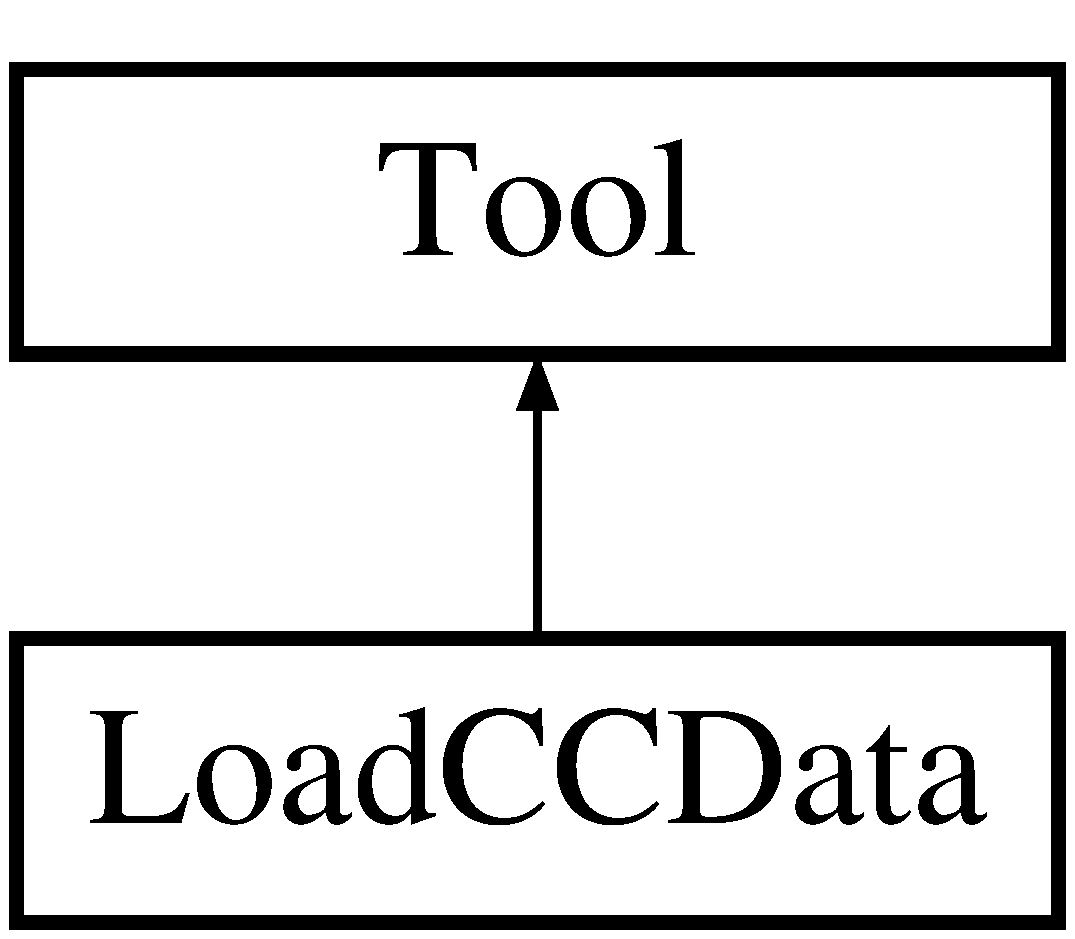
\includegraphics[height=2.000000cm]{classLoadCCData}
\end{center}
\end{figure}
\subsection*{Public Member Functions}
\begin{DoxyCompactItemize}
\item 
\hypertarget{classLoadCCData_ad27ea87d892f247f70f8b96ca67329b1}{bool {\bfseries Initialise} (std\-::string configfile, \hyperlink{classDataModel}{Data\-Model} \&data)}\label{classLoadCCData_ad27ea87d892f247f70f8b96ca67329b1}

\item 
\hypertarget{classLoadCCData_a102f586b9ad192e73b037c764dfd22e0}{bool {\bfseries Execute} ()}\label{classLoadCCData_a102f586b9ad192e73b037c764dfd22e0}

\item 
\hypertarget{classLoadCCData_adab5adee6f15c924a7077d63227e623c}{bool {\bfseries Finalise} ()}\label{classLoadCCData_adab5adee6f15c924a7077d63227e623c}

\end{DoxyCompactItemize}


The documentation for this class was generated from the following files\-:\begin{DoxyCompactItemize}
\item 
User\-Tools/\-Load\-C\-C\-Data/Load\-C\-C\-Data.\-h\item 
User\-Tools/\-Load\-C\-C\-Data/Load\-C\-C\-Data.\-cpp\end{DoxyCompactItemize}

\input{classLoadGeometry}
\hypertarget{classLoadWCSim}{\section{Load\-W\-C\-Sim Class Reference}
\label{classLoadWCSim}\index{Load\-W\-C\-Sim@{Load\-W\-C\-Sim}}
}
Inheritance diagram for Load\-W\-C\-Sim\-:\begin{figure}[H]
\begin{center}
\leavevmode
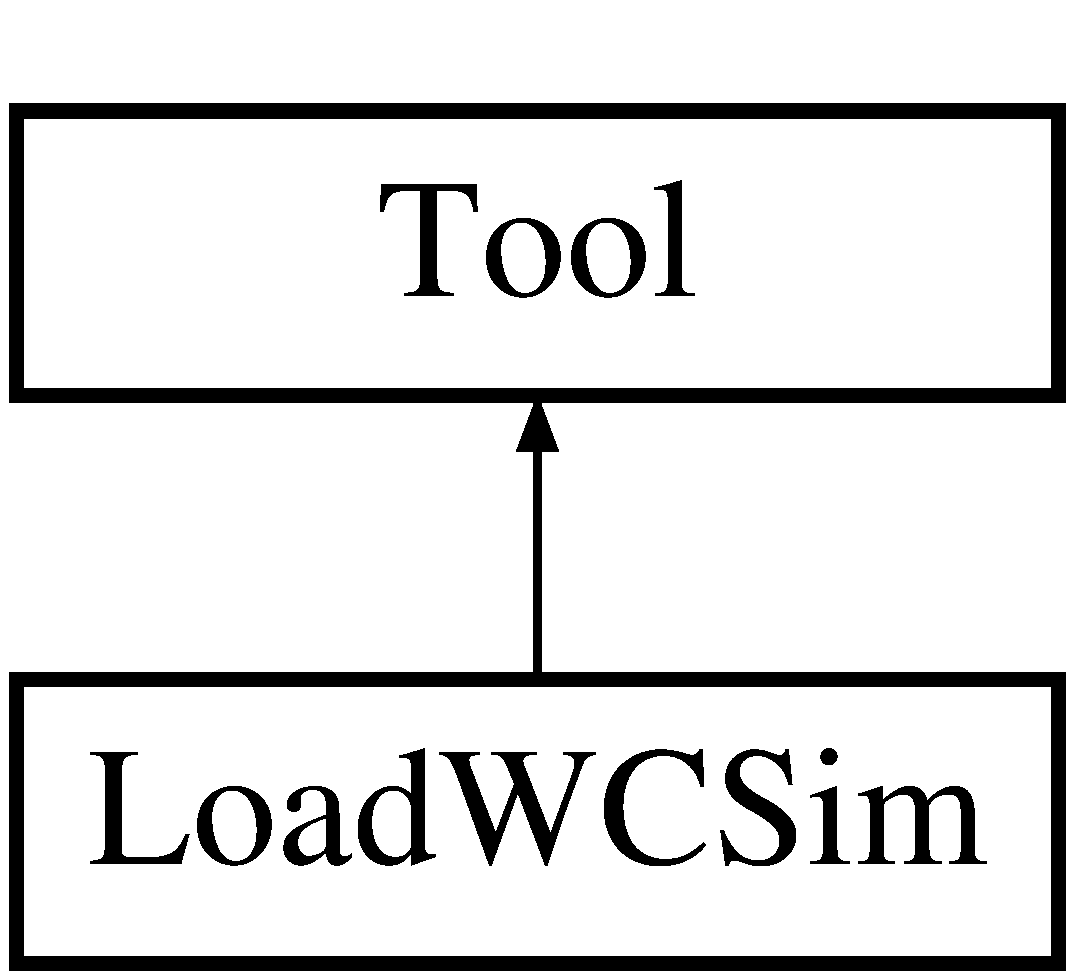
\includegraphics[height=2.000000cm]{classLoadWCSim}
\end{center}
\end{figure}
\subsection*{Public Member Functions}
\begin{DoxyCompactItemize}
\item 
\hypertarget{classLoadWCSim_a14c9d0f26dc099128ca670bd48b7cd34}{bool {\bfseries Initialise} (std\-::string configfile, \hyperlink{classDataModel}{Data\-Model} \&data)}\label{classLoadWCSim_a14c9d0f26dc099128ca670bd48b7cd34}

\item 
\hypertarget{classLoadWCSim_ae8b696ec0cbd3c0febee1c3482df3f7b}{bool {\bfseries Execute} ()}\label{classLoadWCSim_ae8b696ec0cbd3c0febee1c3482df3f7b}

\item 
\hypertarget{classLoadWCSim_afa581b87ca4db35eeb17bab6f40d169f}{bool {\bfseries Finalise} ()}\label{classLoadWCSim_afa581b87ca4db35eeb17bab6f40d169f}

\end{DoxyCompactItemize}


The documentation for this class was generated from the following files\-:\begin{DoxyCompactItemize}
\item 
User\-Tools/\-Load\-W\-C\-Sim/Load\-W\-C\-Sim.\-h\item 
User\-Tools/\-Load\-W\-C\-Sim/Load\-W\-C\-Sim.\-cpp\end{DoxyCompactItemize}

\hypertarget{classLoadWCSimLAPPD}{\section{Load\-W\-C\-Sim\-L\-A\-P\-P\-D Class Reference}
\label{classLoadWCSimLAPPD}\index{Load\-W\-C\-Sim\-L\-A\-P\-P\-D@{Load\-W\-C\-Sim\-L\-A\-P\-P\-D}}
}
Inheritance diagram for Load\-W\-C\-Sim\-L\-A\-P\-P\-D\-:\begin{figure}[H]
\begin{center}
\leavevmode
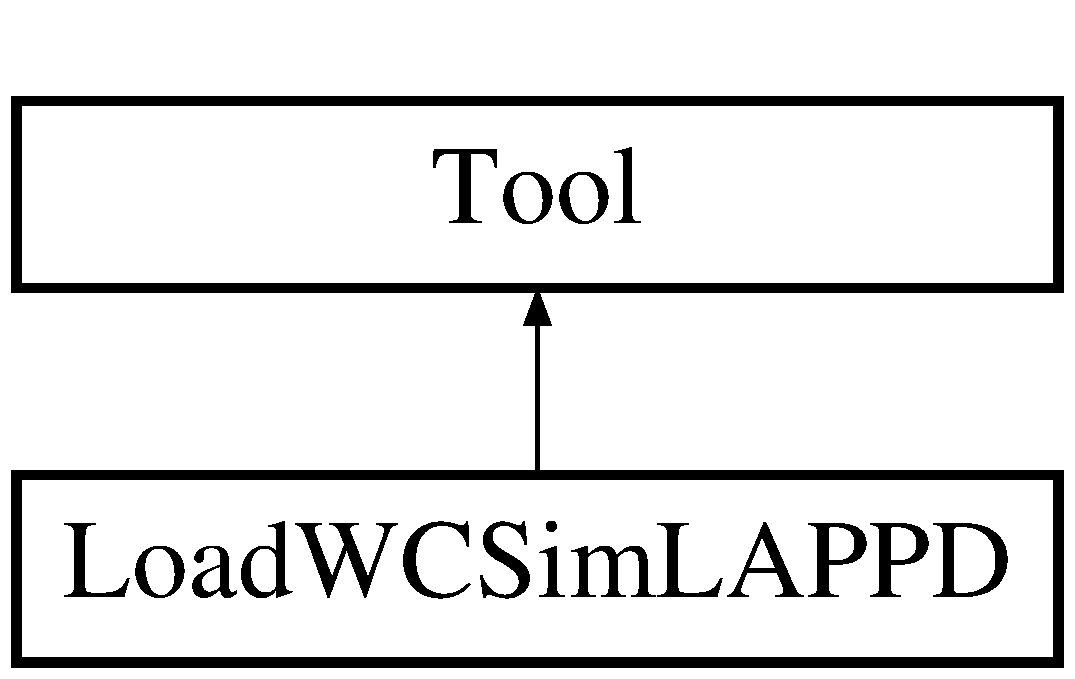
\includegraphics[height=2.000000cm]{classLoadWCSimLAPPD}
\end{center}
\end{figure}
\subsection*{Public Member Functions}
\begin{DoxyCompactItemize}
\item 
\hypertarget{classLoadWCSimLAPPD_a1d2069798a83e0f34f41c4112b2343e8}{bool {\bfseries Initialise} (std\-::string configfile, \hyperlink{classDataModel}{Data\-Model} \&data)}\label{classLoadWCSimLAPPD_a1d2069798a83e0f34f41c4112b2343e8}

\item 
\hypertarget{classLoadWCSimLAPPD_a1b41167086f669fc1a71854a360406da}{bool {\bfseries Execute} ()}\label{classLoadWCSimLAPPD_a1b41167086f669fc1a71854a360406da}

\item 
\hypertarget{classLoadWCSimLAPPD_a457044289ecb5a3d18eeb6e8110a3902}{bool {\bfseries Finalise} ()}\label{classLoadWCSimLAPPD_a457044289ecb5a3d18eeb6e8110a3902}

\end{DoxyCompactItemize}


The documentation for this class was generated from the following files\-:\begin{DoxyCompactItemize}
\item 
User\-Tools/\-Load\-W\-C\-Sim\-L\-A\-P\-P\-D/Load\-W\-C\-Sim\-L\-A\-P\-P\-D.\-h\item 
User\-Tools/\-Load\-W\-C\-Sim\-L\-A\-P\-P\-D/Load\-W\-C\-Sim\-L\-A\-P\-P\-D.\-cpp\end{DoxyCompactItemize}

\hypertarget{classMCHit}{
\section{MCHit Class Reference}
\label{classMCHit}\index{MCHit@{MCHit}}
}
Inheritance diagram for MCHit::\begin{figure}[H]
\begin{center}
\leavevmode
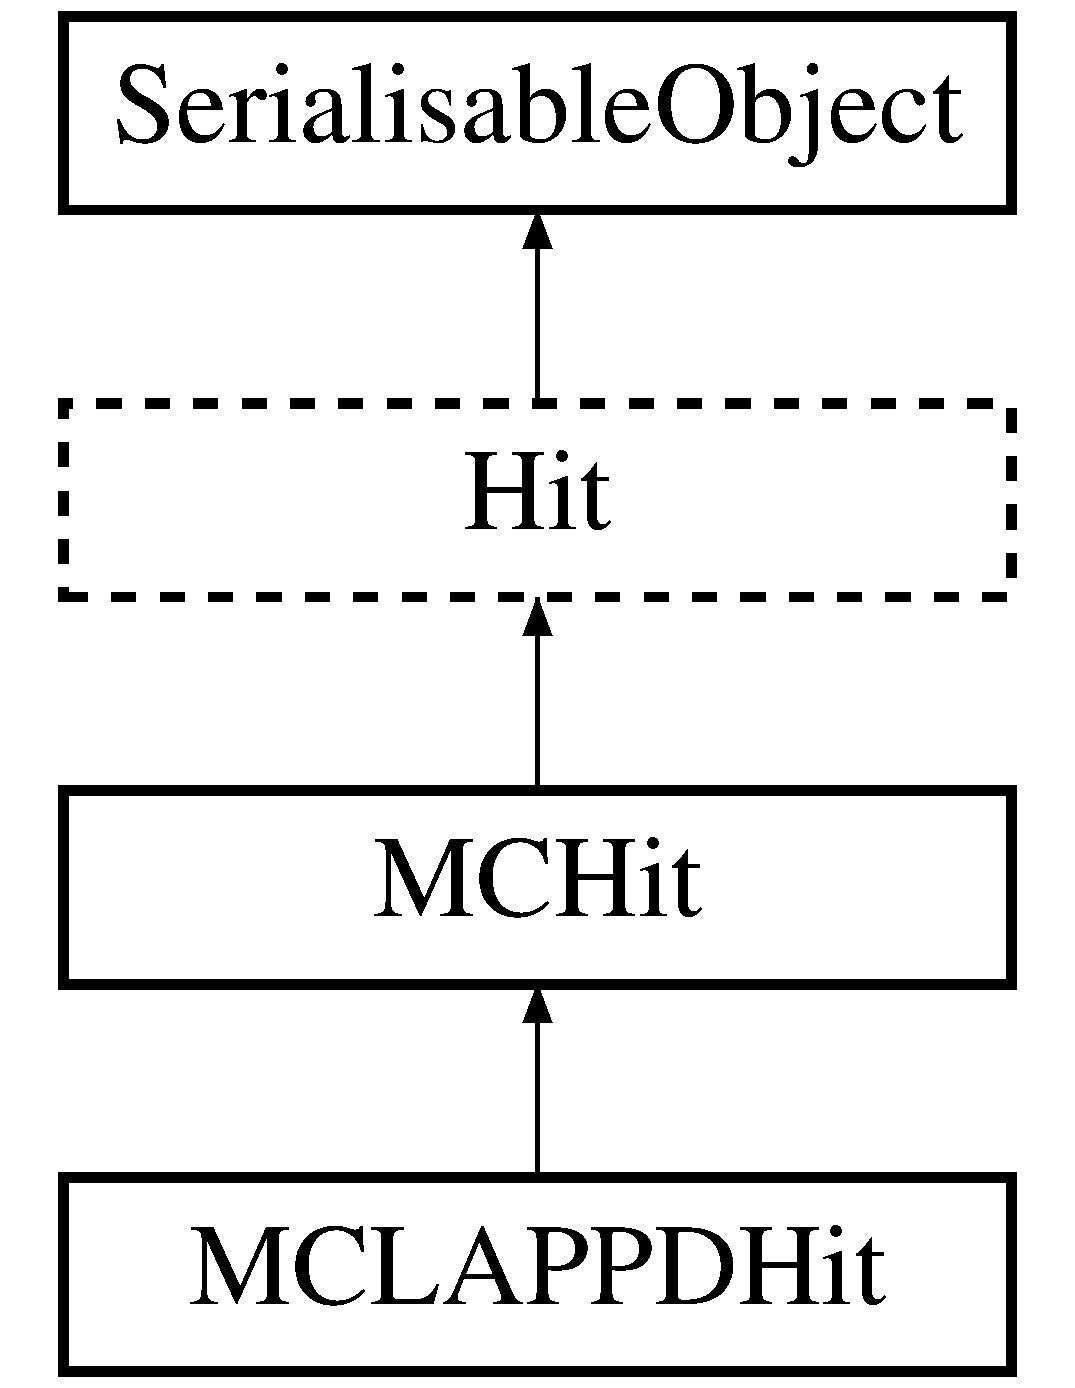
\includegraphics[height=3cm]{classMCHit}
\end{center}
\end{figure}
\subsection*{Public Member Functions}
\begin{DoxyCompactItemize}
\item 
\hypertarget{classMCHit_ab181776ddc1604f20df5799796a76a50}{
{\bfseries Parents} (theparents)}
\label{classMCHit_ab181776ddc1604f20df5799796a76a50}

\item 
\hypertarget{classMCHit_af2a1f4ef53e27bd1c5962a1b61c784d0}{
const std::vector$<$ int $>$ $\ast$ {\bfseries GetParents} () const }
\label{classMCHit_af2a1f4ef53e27bd1c5962a1b61c784d0}

\item 
\hypertarget{classMCHit_a18ae6be9fd39527f915e628ffe65dbec}{
void {\bfseries SetParents} (std::vector$<$ int $>$ parentsin)}
\label{classMCHit_a18ae6be9fd39527f915e628ffe65dbec}

\item 
\hypertarget{classMCHit_a2d016ae3a18d9194a9a45a890f978833}{
bool {\bfseries Print} ()}
\label{classMCHit_a2d016ae3a18d9194a9a45a890f978833}

\end{DoxyCompactItemize}
\subsection*{Protected Member Functions}
\begin{DoxyCompactItemize}
\item 
\hypertarget{classMCHit_ac3213655292d2ae1956ce76bf7bf1fa6}{
{\footnotesize template$<$class Archive $>$ }\\void {\bfseries serialize} (Archive \&ar, const unsigned int version)}
\label{classMCHit_ac3213655292d2ae1956ce76bf7bf1fa6}

\end{DoxyCompactItemize}
\subsection*{Protected Attributes}
\begin{DoxyCompactItemize}
\item 
\hypertarget{classMCHit_a7fbd3892b201ed3790da046e63aed9d5}{
std::vector$<$ int $>$ {\bfseries Parents}}
\label{classMCHit_a7fbd3892b201ed3790da046e63aed9d5}

\end{DoxyCompactItemize}
\subsection*{Friends}
\begin{DoxyCompactItemize}
\item 
\hypertarget{classMCHit_ac98d07dd8f7b70e16ccb9a01abf56b9c}{
class {\bfseries boost::serialization::access}}
\label{classMCHit_ac98d07dd8f7b70e16ccb9a01abf56b9c}

\end{DoxyCompactItemize}


The documentation for this class was generated from the following file:\begin{DoxyCompactItemize}
\item 
DataModel/Hit.h\end{DoxyCompactItemize}

\hypertarget{classMCLAPPDHit}{\section{M\-C\-L\-A\-P\-P\-D\-Hit Class Reference}
\label{classMCLAPPDHit}\index{M\-C\-L\-A\-P\-P\-D\-Hit@{M\-C\-L\-A\-P\-P\-D\-Hit}}
}
Inheritance diagram for M\-C\-L\-A\-P\-P\-D\-Hit\-:\begin{figure}[H]
\begin{center}
\leavevmode
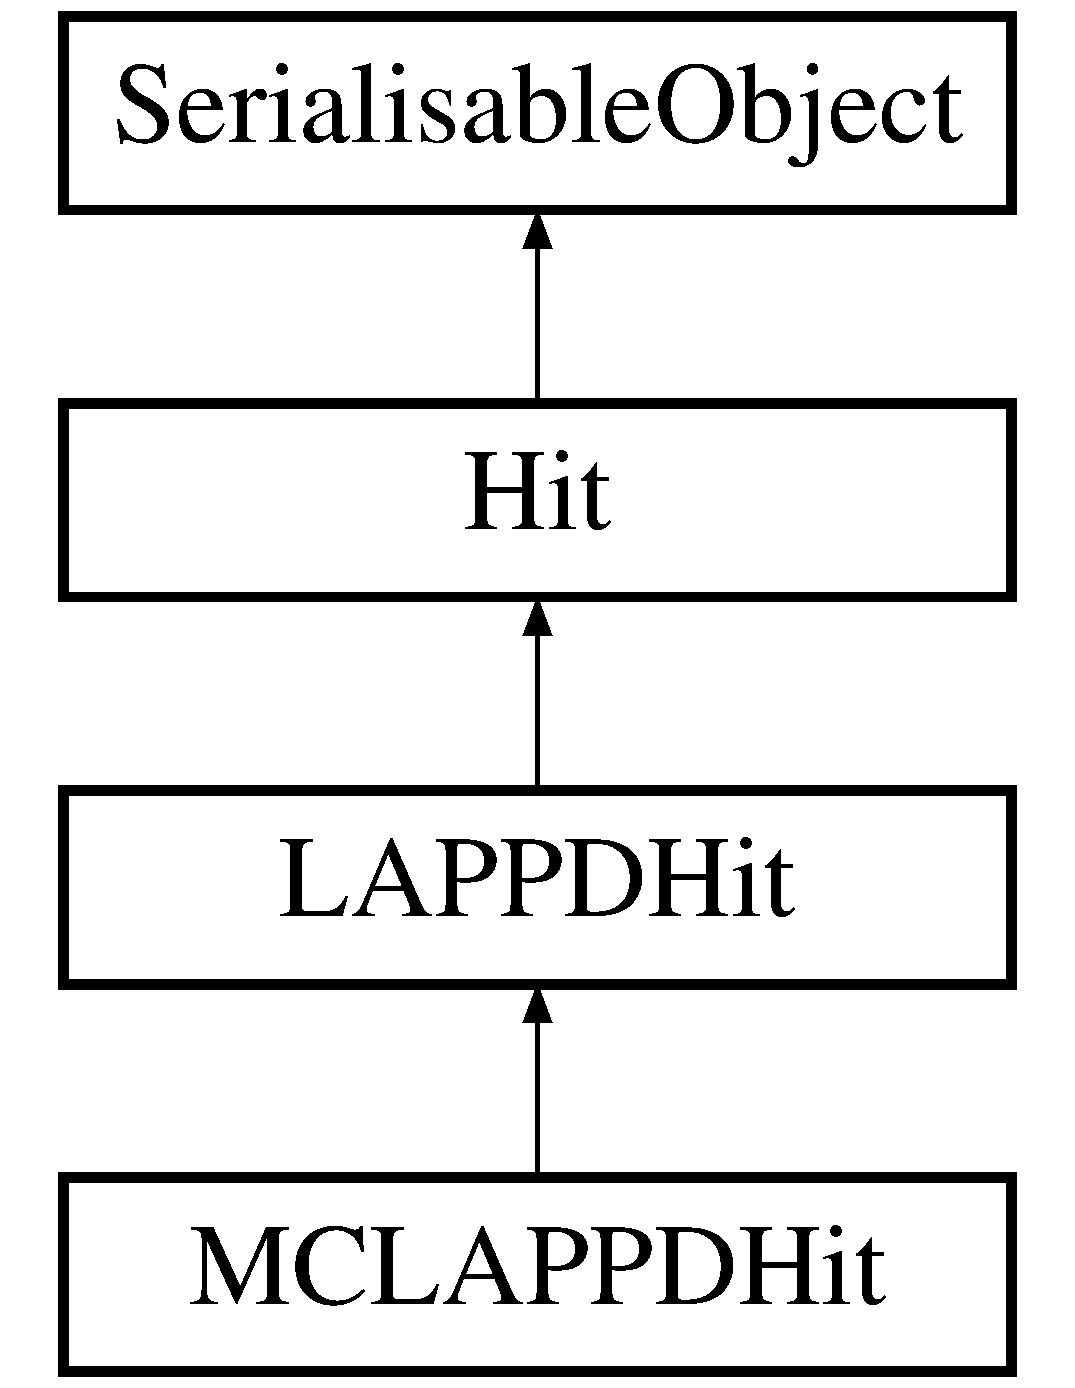
\includegraphics[height=4.000000cm]{classMCLAPPDHit}
\end{center}
\end{figure}
\subsection*{Public Member Functions}
\begin{DoxyCompactItemize}
\item 
\hypertarget{classMCLAPPDHit_ae070e6fd084dffe72b24257fb10eae53}{{\bfseries M\-C\-L\-A\-P\-P\-D\-Hit} (int thetubeid, double thetime, double thecharge, std\-::vector$<$ double $>$ theposition, std\-::vector$<$ double $>$ thelocalposition, std\-::vector$<$ int $>$ theparents)}\label{classMCLAPPDHit_ae070e6fd084dffe72b24257fb10eae53}

\item 
\hypertarget{classMCLAPPDHit_a2cd53e715b43962eece869e296f0efdb}{const std\-::vector$<$ int $>$ $\ast$ {\bfseries Get\-Parents} () const }\label{classMCLAPPDHit_a2cd53e715b43962eece869e296f0efdb}

\item 
\hypertarget{classMCLAPPDHit_a1edf49747c6858e203a3185ec0f656a4}{void {\bfseries Set\-Parents} (std\-::vector$<$ int $>$ parentsin)}\label{classMCLAPPDHit_a1edf49747c6858e203a3185ec0f656a4}

\item 
\hypertarget{classMCLAPPDHit_a90639fe126043eeb4222860265d0e3c5}{bool {\bfseries Print} ()}\label{classMCLAPPDHit_a90639fe126043eeb4222860265d0e3c5}

\item 
\hypertarget{classMCLAPPDHit_a1f0112b487a84fdc753c76bd3429bc06}{{\footnotesize template$<$class Archive $>$ }\\void {\bfseries serialize} (Archive \&ar, const unsigned int version)}\label{classMCLAPPDHit_a1f0112b487a84fdc753c76bd3429bc06}

\end{DoxyCompactItemize}
\subsection*{Protected Attributes}
\begin{DoxyCompactItemize}
\item 
\hypertarget{classMCLAPPDHit_af7f2b72e3e33a3037b5a23b3441c7ce5}{std\-::vector$<$ int $>$ {\bfseries Parents}}\label{classMCLAPPDHit_af7f2b72e3e33a3037b5a23b3441c7ce5}

\end{DoxyCompactItemize}
\subsection*{Friends}
\begin{DoxyCompactItemize}
\item 
\hypertarget{classMCLAPPDHit_ac98d07dd8f7b70e16ccb9a01abf56b9c}{class {\bfseries boost\-::serialization\-::access}}\label{classMCLAPPDHit_ac98d07dd8f7b70e16ccb9a01abf56b9c}

\end{DoxyCompactItemize}
\subsection*{Additional Inherited Members}


The documentation for this class was generated from the following file\-:\begin{DoxyCompactItemize}
\item 
Data\-Model/L\-A\-P\-P\-D\-Hit.\-h\end{DoxyCompactItemize}

\hypertarget{classMCParticle}{\section{M\-C\-Particle Class Reference}
\label{classMCParticle}\index{M\-C\-Particle@{M\-C\-Particle}}
}
Inheritance diagram for M\-C\-Particle\-:\begin{figure}[H]
\begin{center}
\leavevmode
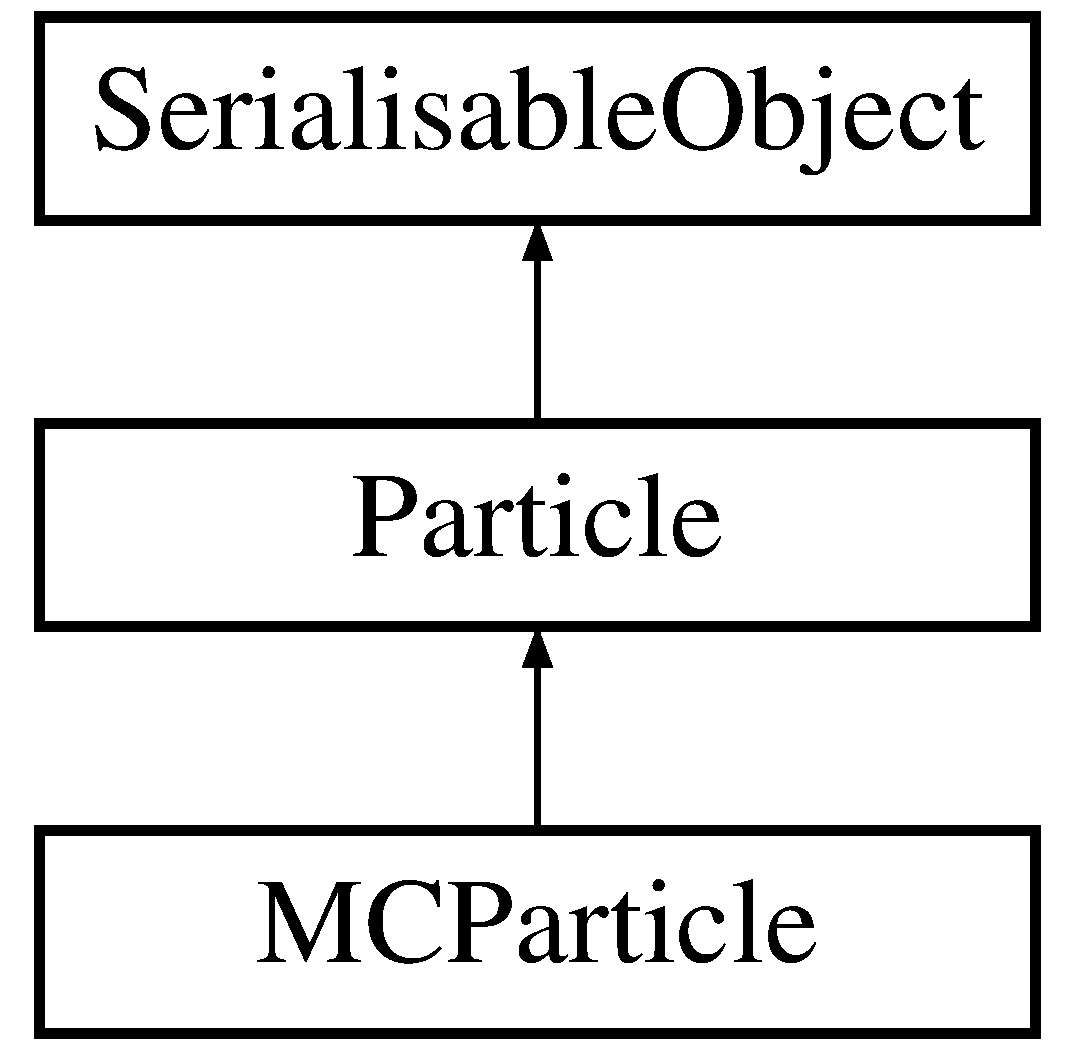
\includegraphics[height=3.000000cm]{classMCParticle}
\end{center}
\end{figure}
\subsection*{Public Member Functions}
\begin{DoxyCompactItemize}
\item 
\hypertarget{classMCParticle_a1e2054a5aa6978bec68fa15133e9aae9}{{\bfseries M\-C\-Particle} (int pdg, double stt\-E, double stp\-E, \hyperlink{classPosition}{Position} sttpos, \hyperlink{classPosition}{Position} stppos, double sttt, double stpt, \hyperlink{classDirection}{Direction} startdir, double len, tracktype tracktypein, int partid, int parentpdg, int flagid)}\label{classMCParticle_a1e2054a5aa6978bec68fa15133e9aae9}

\item 
\hypertarget{classMCParticle_a351d384bc2af0918ece85ba38c9551b2}{int {\bfseries Get\-Particle\-I\-D} ()}\label{classMCParticle_a351d384bc2af0918ece85ba38c9551b2}

\item 
\hypertarget{classMCParticle_a05c2ded23b19858448647ce9d2ba36fd}{int {\bfseries Get\-Parent\-Pdg} ()}\label{classMCParticle_a05c2ded23b19858448647ce9d2ba36fd}

\item 
\hypertarget{classMCParticle_a3240caaaac37a2d4ab3ef5d57aa53e74}{int {\bfseries Get\-Flag} ()}\label{classMCParticle_a3240caaaac37a2d4ab3ef5d57aa53e74}

\item 
\hypertarget{classMCParticle_a1829807b49dda47903441234983df064}{bool {\bfseries Get\-Starts\-In\-Fiducial\-Volume} ()}\label{classMCParticle_a1829807b49dda47903441234983df064}

\item 
\hypertarget{classMCParticle_a99c79b20440359ee841296eff1a4ab61}{double {\bfseries Get\-Track\-Angle\-X} ()}\label{classMCParticle_a99c79b20440359ee841296eff1a4ab61}

\item 
\hypertarget{classMCParticle_a98e706fd77669b0461e739b5a8e46998}{double {\bfseries Get\-Track\-Angle\-Y} ()}\label{classMCParticle_a98e706fd77669b0461e739b5a8e46998}

\item 
\hypertarget{classMCParticle_ae5bbdd4456fb3131ec6eb7213cab54cb}{double {\bfseries Get\-Track\-Angle\-From\-Beam} ()}\label{classMCParticle_ae5bbdd4456fb3131ec6eb7213cab54cb}

\item 
\hypertarget{classMCParticle_aa9626a1846b63292b5356fe2be097fe9}{bool {\bfseries Get\-Enters\-Tank} ()}\label{classMCParticle_aa9626a1846b63292b5356fe2be097fe9}

\item 
\hypertarget{classMCParticle_a112df02772c9bc084298a54b86212133}{\hyperlink{classPosition}{Position} {\bfseries Get\-Tank\-Entry\-Point} ()}\label{classMCParticle_a112df02772c9bc084298a54b86212133}

\item 
\hypertarget{classMCParticle_a6a7562aabf349e90c0e1e3751189e5eb}{bool {\bfseries Get\-Exits\-Tank} ()}\label{classMCParticle_a6a7562aabf349e90c0e1e3751189e5eb}

\item 
\hypertarget{classMCParticle_a6693f8f91b1ecab9309ffb752f5fcd66}{\hyperlink{classPosition}{Position} {\bfseries Get\-Tank\-Exit\-Point} ()}\label{classMCParticle_a6693f8f91b1ecab9309ffb752f5fcd66}

\item 
\hypertarget{classMCParticle_a9137f3783a143643ef16b3b63fdabef8}{double {\bfseries Get\-Track\-Length\-In\-Tank} ()}\label{classMCParticle_a9137f3783a143643ef16b3b63fdabef8}

\item 
\hypertarget{classMCParticle_a6b69dd58bc549a57cc780a9621c8fcad}{bool {\bfseries Get\-Enters\-Mrd} ()}\label{classMCParticle_a6b69dd58bc549a57cc780a9621c8fcad}

\item 
\hypertarget{classMCParticle_a4fc1d825ca0b6898323718e382574df0}{\hyperlink{classPosition}{Position} {\bfseries Get\-Mrd\-Entry\-Point} ()}\label{classMCParticle_a4fc1d825ca0b6898323718e382574df0}

\item 
\hypertarget{classMCParticle_a5f529c1629fdaf94d6061d1bde2013bc}{bool {\bfseries Get\-Exits\-Mrd} ()}\label{classMCParticle_a5f529c1629fdaf94d6061d1bde2013bc}

\item 
\hypertarget{classMCParticle_a33f74539498e327f17345f5801b9ce60}{\hyperlink{classPosition}{Position} {\bfseries Get\-Mrd\-Exit\-Point} ()}\label{classMCParticle_a33f74539498e327f17345f5801b9ce60}

\item 
\hypertarget{classMCParticle_ab4172cbc5024701f1286ec9b3cdae9a7}{bool {\bfseries Get\-Penetrates\-Mrd} ()}\label{classMCParticle_ab4172cbc5024701f1286ec9b3cdae9a7}

\item 
\hypertarget{classMCParticle_a46bf3f4fb48252b4f459b77b108a8e67}{double {\bfseries Get\-Track\-Length\-In\-Mrd} ()}\label{classMCParticle_a46bf3f4fb48252b4f459b77b108a8e67}

\item 
\hypertarget{classMCParticle_a3d260af122ff90824de2e2be7f672f07}{double {\bfseries Get\-Mrd\-Penetration} ()}\label{classMCParticle_a3d260af122ff90824de2e2be7f672f07}

\item 
\hypertarget{classMCParticle_afa08a1cb74a4b0b642f0b62c04114976}{int {\bfseries Get\-Num\-Mrd\-Layers\-Penetrated} ()}\label{classMCParticle_afa08a1cb74a4b0b642f0b62c04114976}

\item 
\hypertarget{classMCParticle_ac8325eb8dd7e2d10b6b406dfcd6b31af}{double {\bfseries Get\-Mrd\-Energy\-Loss} ()}\label{classMCParticle_ac8325eb8dd7e2d10b6b406dfcd6b31af}

\item 
\hypertarget{classMCParticle_ab3f8776c846fcc1c82f2d9083beaf07f}{void {\bfseries Set\-Particle\-I\-D} (int partidin)}\label{classMCParticle_ab3f8776c846fcc1c82f2d9083beaf07f}

\item 
\hypertarget{classMCParticle_a835ce089d630c4624a3060980450ca2c}{void {\bfseries Set\-Parent\-Pdg} (int parentpdgin)}\label{classMCParticle_a835ce089d630c4624a3060980450ca2c}

\item 
\hypertarget{classMCParticle_ace8eaad4c1fd7398fb5bda3316b5395b}{void {\bfseries Set\-Flag} (int flagidin)}\label{classMCParticle_ace8eaad4c1fd7398fb5bda3316b5395b}

\item 
\hypertarget{classMCParticle_a2a42a4f6ef9af8a6158e422680a57b47}{void {\bfseries Set\-Starts\-In\-Fiducial\-Volume} (bool i\-Starts\-In\-Fiducial\-Volume)}\label{classMCParticle_a2a42a4f6ef9af8a6158e422680a57b47}

\item 
\hypertarget{classMCParticle_a1fb1b9c4206de10c602b1095e6428578}{void {\bfseries Set\-Enters\-Tank} (bool i\-Enters\-Tank)}\label{classMCParticle_a1fb1b9c4206de10c602b1095e6428578}

\item 
\hypertarget{classMCParticle_a2cfded14729766192df1b9770edba92a}{void {\bfseries Set\-Tank\-Entry\-Point} (\hyperlink{classPosition}{Position} i\-Tank\-Entry\-Point)}\label{classMCParticle_a2cfded14729766192df1b9770edba92a}

\item 
\hypertarget{classMCParticle_a702069712afdc032362de66c133c0165}{void {\bfseries Set\-Exits\-Tank} (bool i\-Exits\-Tank)}\label{classMCParticle_a702069712afdc032362de66c133c0165}

\item 
\hypertarget{classMCParticle_a1cbf3a6c05ac82ec5e9c8b90a70c2940}{void {\bfseries Set\-Tank\-Exit\-Point} (\hyperlink{classPosition}{Position} i\-Tank\-Exit\-Point)}\label{classMCParticle_a1cbf3a6c05ac82ec5e9c8b90a70c2940}

\item 
\hypertarget{classMCParticle_a7ca9800559d1e4fddd3fc98c0deb2c99}{void {\bfseries Set\-Track\-Length\-In\-Tank} (double i\-Track\-Length\-In\-Tank)}\label{classMCParticle_a7ca9800559d1e4fddd3fc98c0deb2c99}

\item 
\hypertarget{classMCParticle_a0538d9cb8cf49a824f3fd77d0531e935}{void {\bfseries Set\-Enters\-Mrd} (bool i\-Enters\-Mrd)}\label{classMCParticle_a0538d9cb8cf49a824f3fd77d0531e935}

\item 
\hypertarget{classMCParticle_a5ac43b6d4e343123b0308aeff287a1ec}{void {\bfseries Set\-Mrd\-Entry\-Point} (\hyperlink{classPosition}{Position} i\-Mrd\-Entry\-Point)}\label{classMCParticle_a5ac43b6d4e343123b0308aeff287a1ec}

\item 
\hypertarget{classMCParticle_ad11395d2bd739fc1ad5d473f6313a34a}{void {\bfseries Set\-Exits\-Mrd} (bool i\-Exits\-Mrd)}\label{classMCParticle_ad11395d2bd739fc1ad5d473f6313a34a}

\item 
\hypertarget{classMCParticle_a775d17a50fd84cd07f9049aff86f0ead}{void {\bfseries Set\-Mrd\-Exit\-Point} (\hyperlink{classPosition}{Position} i\-Mrd\-Exit\-Point)}\label{classMCParticle_a775d17a50fd84cd07f9049aff86f0ead}

\item 
\hypertarget{classMCParticle_ab112ca1f301435bb933ba813d7a4da3e}{void {\bfseries Set\-Penetrates\-Mrd} (bool i\-Penetrates\-Mrd)}\label{classMCParticle_ab112ca1f301435bb933ba813d7a4da3e}

\item 
\hypertarget{classMCParticle_af85b13f2164e52e752d6e14534d4b31c}{void {\bfseries Set\-Track\-Length\-In\-Mrd} (double i\-Track\-Length\-In\-Mrd)}\label{classMCParticle_af85b13f2164e52e752d6e14534d4b31c}

\item 
\hypertarget{classMCParticle_a1bd0d632655c48ee8bc311b7ab9c3996}{void {\bfseries Set\-Mrd\-Penetration} (double i\-Mrd\-Penetration)}\label{classMCParticle_a1bd0d632655c48ee8bc311b7ab9c3996}

\item 
\hypertarget{classMCParticle_abc4ac222c79d03dd421dccf1c27aa461}{void {\bfseries Set\-Num\-Mrd\-Layers\-Penetrated} (int i\-Mrd\-Layers\-Penetrated)}\label{classMCParticle_abc4ac222c79d03dd421dccf1c27aa461}

\item 
\hypertarget{classMCParticle_a3db0d00c918e435c4cacc51e80fad7db}{void {\bfseries Set\-Mrd\-Energy\-Loss} (double i\-Mrd\-Energy\-Loss)}\label{classMCParticle_a3db0d00c918e435c4cacc51e80fad7db}

\item 
\hypertarget{classMCParticle_abc9a006d2fb4c95ca7f08fa218867c21}{void {\bfseries Set\-Track\-Angle\-X} (double i\-Track\-Angle\-X)}\label{classMCParticle_abc9a006d2fb4c95ca7f08fa218867c21}

\item 
\hypertarget{classMCParticle_af39b59b0cde215f2a6fe2183d8c580b9}{void {\bfseries Set\-Track\-Angle\-Y} (double i\-Track\-Angle\-Y)}\label{classMCParticle_af39b59b0cde215f2a6fe2183d8c580b9}

\item 
\hypertarget{classMCParticle_af278f6d766d7a4cc4818ae0b3e64f73f}{void {\bfseries Set\-Track\-Angle\-From\-Beam} (double i\-Track\-Angle\-From\-Beam)}\label{classMCParticle_af278f6d766d7a4cc4818ae0b3e64f73f}

\item 
\hypertarget{classMCParticle_a1691c5d5d847e0a2419cdad793ff2ddb}{bool {\bfseries Get\-World\-Contained} (int startstop, \hyperlink{classPosition}{Position} a\-Vertex=\hyperlink{classPosition}{Position}(0, 0, 0))}\label{classMCParticle_a1691c5d5d847e0a2419cdad793ff2ddb}

\item 
\hypertarget{classMCParticle_a602114887228de2afbfcd0a31ddba66c}{bool {\bfseries Print} ()}\label{classMCParticle_a602114887228de2afbfcd0a31ddba66c}

\end{DoxyCompactItemize}
\subsection*{Protected Member Functions}
\begin{DoxyCompactItemize}
\item 
\hypertarget{classMCParticle_ac28878d706363533ac74f18faf272fb4}{{\footnotesize template$<$class Archive $>$ }\\void {\bfseries serialize} (Archive \&ar, const unsigned int version)}\label{classMCParticle_ac28878d706363533ac74f18faf272fb4}

\end{DoxyCompactItemize}
\subsection*{Protected Attributes}
\begin{DoxyCompactItemize}
\item 
\hypertarget{classMCParticle_a52ca5b486dd9ded3b7da2b77c2704f85}{int {\bfseries Particle\-I\-D}}\label{classMCParticle_a52ca5b486dd9ded3b7da2b77c2704f85}

\item 
\hypertarget{classMCParticle_aa60d9c88e4c168be89a8075414078e82}{int {\bfseries Parent\-Pdg}}\label{classMCParticle_aa60d9c88e4c168be89a8075414078e82}

\item 
\hypertarget{classMCParticle_a74ff96a2e3f2c92d991a631dc320b343}{int {\bfseries Flag}}\label{classMCParticle_a74ff96a2e3f2c92d991a631dc320b343}

\item 
\hypertarget{classMCParticle_a9328c826d1ee1d615e312d25235d04a0}{bool {\bfseries Starts\-In\-Fiducial\-Volume}}\label{classMCParticle_a9328c826d1ee1d615e312d25235d04a0}

\item 
\hypertarget{classMCParticle_aafb0416bfa7dfcaa14f4243d76930239}{double {\bfseries Track\-Angle\-X}}\label{classMCParticle_aafb0416bfa7dfcaa14f4243d76930239}

\item 
\hypertarget{classMCParticle_aaf4a5cd3469f3d527c0ac8f4e3713c4b}{double {\bfseries Track\-Angle\-Y}}\label{classMCParticle_aaf4a5cd3469f3d527c0ac8f4e3713c4b}

\item 
\hypertarget{classMCParticle_af4cdfb96769ec1a40e45c4f40b9eb520}{double {\bfseries Track\-Angle\-From\-Beam}}\label{classMCParticle_af4cdfb96769ec1a40e45c4f40b9eb520}

\item 
\hypertarget{classMCParticle_afc38d81f454f0011d513db8dedc39d37}{bool {\bfseries Enters\-Tank}}\label{classMCParticle_afc38d81f454f0011d513db8dedc39d37}

\item 
\hypertarget{classMCParticle_ad1c64ca6b80955ea88cc1014360c53fa}{\hyperlink{classPosition}{Position} {\bfseries Tank\-Entry\-Point}}\label{classMCParticle_ad1c64ca6b80955ea88cc1014360c53fa}

\item 
\hypertarget{classMCParticle_aa33826267b580a0e0083df6deaeb26ce}{bool {\bfseries Exits\-Tank}}\label{classMCParticle_aa33826267b580a0e0083df6deaeb26ce}

\item 
\hypertarget{classMCParticle_a9d57e7bfd963f6ee5cdf4de16b15652f}{\hyperlink{classPosition}{Position} {\bfseries Tank\-Exit\-Point}}\label{classMCParticle_a9d57e7bfd963f6ee5cdf4de16b15652f}

\item 
\hypertarget{classMCParticle_a3a178c1eab5c3e1baca3d7416066cff5}{double {\bfseries Track\-Length\-In\-Tank}}\label{classMCParticle_a3a178c1eab5c3e1baca3d7416066cff5}

\item 
\hypertarget{classMCParticle_aca01ce3d68f3eb4fa1aea0e052da2322}{double {\bfseries Enters\-Mrd}}\label{classMCParticle_aca01ce3d68f3eb4fa1aea0e052da2322}

\item 
\hypertarget{classMCParticle_a06f90a30827626e16ce036b725032424}{\hyperlink{classPosition}{Position} {\bfseries Mrd\-Entry\-Point}}\label{classMCParticle_a06f90a30827626e16ce036b725032424}

\item 
\hypertarget{classMCParticle_ac2690fd0362dcad58682cda54179035c}{bool {\bfseries Exits\-Mrd}}\label{classMCParticle_ac2690fd0362dcad58682cda54179035c}

\item 
\hypertarget{classMCParticle_a79fe95c4ab5a161f31f42809dda35d8e}{\hyperlink{classPosition}{Position} {\bfseries Mrd\-Exit\-Point}}\label{classMCParticle_a79fe95c4ab5a161f31f42809dda35d8e}

\item 
\hypertarget{classMCParticle_ad82f8f04628606c79b789cdaad72c73d}{bool {\bfseries Penetrates\-Mrd}}\label{classMCParticle_ad82f8f04628606c79b789cdaad72c73d}

\item 
\hypertarget{classMCParticle_affee0c98fd66da0ce6c704fee413b120}{double {\bfseries Track\-Length\-In\-Mrd}}\label{classMCParticle_affee0c98fd66da0ce6c704fee413b120}

\item 
\hypertarget{classMCParticle_aae98f51a041e389e7439cfe2229e1936}{double {\bfseries Mrd\-Penetration}}\label{classMCParticle_aae98f51a041e389e7439cfe2229e1936}

\item 
\hypertarget{classMCParticle_ae3e7da6821154bc8a5817e87ec10b6ea}{int {\bfseries Mrd\-Layers\-Penetrated}}\label{classMCParticle_ae3e7da6821154bc8a5817e87ec10b6ea}

\item 
\hypertarget{classMCParticle_a4c8a5b9e7d2f4268fa4a60e5d80dcc22}{double {\bfseries Mrd\-Energy\-Loss}}\label{classMCParticle_a4c8a5b9e7d2f4268fa4a60e5d80dcc22}

\end{DoxyCompactItemize}
\subsection*{Friends}
\begin{DoxyCompactItemize}
\item 
\hypertarget{classMCParticle_ac98d07dd8f7b70e16ccb9a01abf56b9c}{class {\bfseries boost\-::serialization\-::access}}\label{classMCParticle_ac98d07dd8f7b70e16ccb9a01abf56b9c}

\end{DoxyCompactItemize}
\subsection*{Additional Inherited Members}


The documentation for this class was generated from the following file\-:\begin{DoxyCompactItemize}
\item 
Data\-Model/Particle.\-h\end{DoxyCompactItemize}

\hypertarget{classMCParticleProperties}{
\section{MCParticleProperties Class Reference}
\label{classMCParticleProperties}\index{MCParticleProperties@{MCParticleProperties}}
}
\subsection*{Public Member Functions}
\begin{DoxyCompactItemize}
\item 
\hypertarget{classMCParticleProperties_aeb42d506b628e71bad8d15c6d20b7728}{
bool {\bfseries Initialise} (std::string configfile, \hyperlink{classDataModel}{DataModel} \&data)}
\label{classMCParticleProperties_aeb42d506b628e71bad8d15c6d20b7728}

\item 
\hypertarget{classMCParticleProperties_a93cf4884b81b864d9a40ae53689ad9f8}{
bool {\bfseries Execute} ()}
\label{classMCParticleProperties_a93cf4884b81b864d9a40ae53689ad9f8}

\item 
\hypertarget{classMCParticleProperties_a6ed9e609a5194be6d1c2461759b086f1}{
bool {\bfseries Finalise} ()}
\label{classMCParticleProperties_a6ed9e609a5194be6d1c2461759b086f1}

\end{DoxyCompactItemize}


The documentation for this class was generated from the following files:\begin{DoxyCompactItemize}
\item 
UserTools/MCParticleProperties/MCParticleProperties.h\item 
UserTools/MCParticleProperties/MCParticleProperties.cpp\end{DoxyCompactItemize}

\hypertarget{classMCRecoEventLoader}{\section{M\-C\-Reco\-Event\-Loader Class Reference}
\label{classMCRecoEventLoader}\index{M\-C\-Reco\-Event\-Loader@{M\-C\-Reco\-Event\-Loader}}
}
Inheritance diagram for M\-C\-Reco\-Event\-Loader\-:\begin{figure}[H]
\begin{center}
\leavevmode
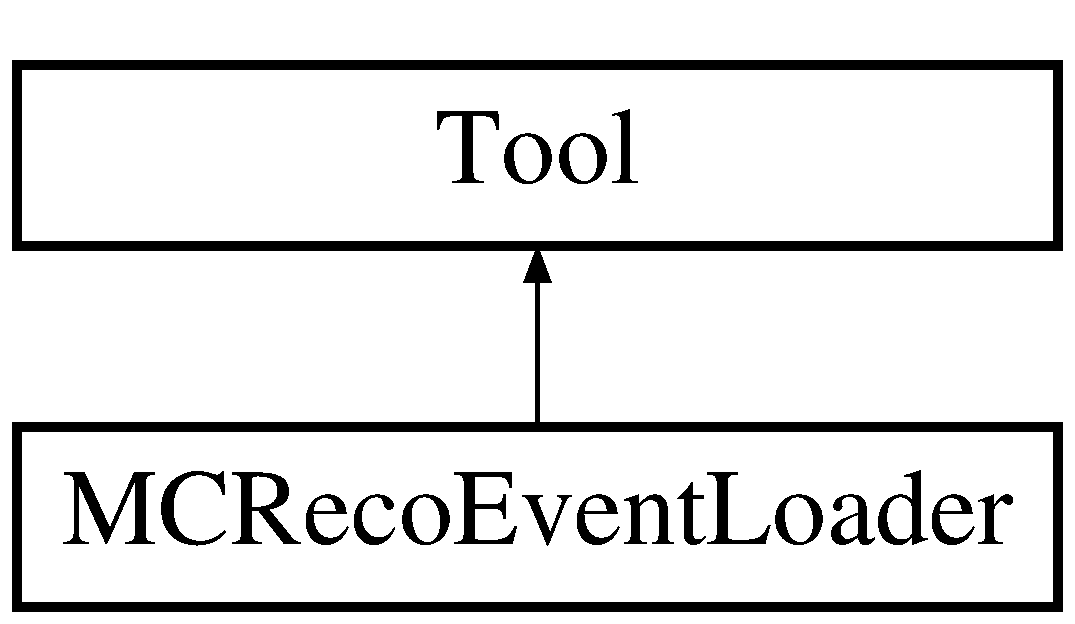
\includegraphics[height=2.000000cm]{classMCRecoEventLoader}
\end{center}
\end{figure}
\subsection*{Public Member Functions}
\begin{DoxyCompactItemize}
\item 
bool \hyperlink{classMCRecoEventLoader_a3c57d089982246d613d553092ab8f141}{Initialise} (std\-::string configfile, \hyperlink{classDataModel}{Data\-Model} \&data)
\item 
bool \hyperlink{classMCRecoEventLoader_a17027f8a3689b459fa54a4a3c84b5a0c}{Execute} ()
\item 
\hypertarget{classMCRecoEventLoader_ac4b21a91ed4795b7ffc9695ec38438e2}{bool {\bfseries Finalise} ()}\label{classMCRecoEventLoader_ac4b21a91ed4795b7ffc9695ec38438e2}

\item 
void \hyperlink{classMCRecoEventLoader_a981fbf41206f4be37c40ec5fbaeb9c9d}{Find\-True\-Vertex\-From\-M\-C} ()
\begin{DoxyCompactList}\small\item\em Find true neutrino vertex. \end{DoxyCompactList}\item 
void \hyperlink{classMCRecoEventLoader_ade2e70b075295f19384e6862dda123ec}{Find\-Pion\-Kaon\-Count\-From\-M\-C} ()
\begin{DoxyCompactList}\small\item\em Find Pion\-Kaon Count. \end{DoxyCompactList}\item 
void \hyperlink{classMCRecoEventLoader_a4d3d3f6e9b15bd07420b0b10f04eed11}{Push\-True\-Vertex} (bool savetodisk)
\begin{DoxyCompactList}\small\item\em Save true neutrino vertex. \end{DoxyCompactList}\item 
void \hyperlink{classMCRecoEventLoader_a57ec5fa238eed8885465bf6d3e03078c}{Push\-True\-Stop\-Vertex} (bool savetodisk)
\begin{DoxyCompactList}\small\item\em Save true neutrino vertex. \end{DoxyCompactList}\item 
void \hyperlink{classMCRecoEventLoader_a79a348512d9c7fb13aa86e96d5f1d39b}{Push\-True\-Water\-Track\-Length} (double Water\-T)
\begin{DoxyCompactList}\small\item\em Push muon track lengths to Reco\-Event Store. \end{DoxyCompactList}\item 
void \hyperlink{classMCRecoEventLoader_a258d351d5afce9a2be153db10a80ae3a}{Push\-True\-M\-R\-D\-Track\-Length} (double M\-R\-D\-T)
\item 
void \hyperlink{classMCRecoEventLoader_a1c01acb2c109e46de4e1dc27911843c3}{Reset} ()
\begin{DoxyCompactList}\small\item\em Reset initialized classes. \end{DoxyCompactList}\end{DoxyCompactItemize}
\subsection*{Public Attributes}
\begin{DoxyCompactItemize}
\item 
\hypertarget{classMCRecoEventLoader_a42b09a53c17f03a6e4fcce20cd4c56b1}{int {\bfseries verbosity} =1}\label{classMCRecoEventLoader_a42b09a53c17f03a6e4fcce20cd4c56b1}

\item 
\hypertarget{classMCRecoEventLoader_a0d3eb072ae7301282ba510bbd11ffb0d}{bool {\bfseries f\-Get\-Pi\-K\-Info}}\label{classMCRecoEventLoader_a0d3eb072ae7301282ba510bbd11ffb0d}

\item 
\hypertarget{classMCRecoEventLoader_ab936432f202a835b7877dbc63303a57c}{int {\bfseries f\-Particle\-I\-D}}\label{classMCRecoEventLoader_ab936432f202a835b7877dbc63303a57c}

\item 
\hypertarget{classMCRecoEventLoader_aefded74813d943854628aa0da13953ff}{double {\bfseries xshift}}\label{classMCRecoEventLoader_aefded74813d943854628aa0da13953ff}

\item 
\hypertarget{classMCRecoEventLoader_a008cd13186e5458c4232376980ff8430}{double {\bfseries yshift}}\label{classMCRecoEventLoader_a008cd13186e5458c4232376980ff8430}

\item 
\hypertarget{classMCRecoEventLoader_a5320937dd08d67c172b0f90956615e11}{double {\bfseries zshift}}\label{classMCRecoEventLoader_a5320937dd08d67c172b0f90956615e11}

\item 
\hypertarget{classMCRecoEventLoader_a06c8c257c06cca00a6b34c51365e6d69}{\hyperlink{classRecoVertex}{Reco\-Vertex} $\ast$ \hyperlink{classMCRecoEventLoader_a06c8c257c06cca00a6b34c51365e6d69}{f\-Muon\-Start\-Vertex} = nullptr}\label{classMCRecoEventLoader_a06c8c257c06cca00a6b34c51365e6d69}

\begin{DoxyCompactList}\small\item\em true muon start vertex \end{DoxyCompactList}\item 
\hypertarget{classMCRecoEventLoader_ab4eb6938d73f33b4d4fbcaccd28f9c65}{\hyperlink{classRecoVertex}{Reco\-Vertex} $\ast$ \hyperlink{classMCRecoEventLoader_ab4eb6938d73f33b4d4fbcaccd28f9c65}{f\-Muon\-Stop\-Vertex} = nullptr}\label{classMCRecoEventLoader_ab4eb6938d73f33b4d4fbcaccd28f9c65}

\begin{DoxyCompactList}\small\item\em true muon stop vertex \end{DoxyCompactList}\item 
\hypertarget{classMCRecoEventLoader_a92922e07f398c491b9fd9e13ef012689}{std\-::vector$<$ \hyperlink{classMCParticle}{M\-C\-Particle} $>$ $\ast$ \hyperlink{classMCRecoEventLoader_a92922e07f398c491b9fd9e13ef012689}{f\-M\-C\-Particles} =nullptr}\label{classMCRecoEventLoader_a92922e07f398c491b9fd9e13ef012689}

\begin{DoxyCompactList}\small\item\em truth tracks \end{DoxyCompactList}\item 
\hypertarget{classMCRecoEventLoader_aca4904cc6f45b2dd128ac58faa6c060d}{double {\bfseries Water\-Track\-Length} = -\/999.}\label{classMCRecoEventLoader_aca4904cc6f45b2dd128ac58faa6c060d}

\item 
\hypertarget{classMCRecoEventLoader_a9460d1064fa3c64c723dec37c834b75b}{double {\bfseries M\-R\-D\-Track\-Length} = -\/999.}\label{classMCRecoEventLoader_a9460d1064fa3c64c723dec37c834b75b}

\item 
\hypertarget{classMCRecoEventLoader_a402d61b93cd42d10500aedeb6e534b5d}{int \hyperlink{classMCRecoEventLoader_a402d61b93cd42d10500aedeb6e534b5d}{v\-\_\-error} =0}\label{classMCRecoEventLoader_a402d61b93cd42d10500aedeb6e534b5d}

\begin{DoxyCompactList}\small\item\em verbosity levels\-: if 'verbosity' $<$ this level, the message type will be logged. \end{DoxyCompactList}\item 
\hypertarget{classMCRecoEventLoader_a4693e8478a38f832b1ea3daff98353a9}{int {\bfseries v\-\_\-warning} =1}\label{classMCRecoEventLoader_a4693e8478a38f832b1ea3daff98353a9}

\item 
\hypertarget{classMCRecoEventLoader_a2e5d293cda46249cbab52275bd52c508}{int {\bfseries v\-\_\-message} =2}\label{classMCRecoEventLoader_a2e5d293cda46249cbab52275bd52c508}

\item 
\hypertarget{classMCRecoEventLoader_a1dd2e7e0076fafe88a4baa4218f772a0}{int {\bfseries v\-\_\-debug} =3}\label{classMCRecoEventLoader_a1dd2e7e0076fafe88a4baa4218f772a0}

\item 
\hypertarget{classMCRecoEventLoader_a1c2cc6580cbfcad49ea1cd17e7ce08f3}{std\-::string {\bfseries logmessage}}\label{classMCRecoEventLoader_a1c2cc6580cbfcad49ea1cd17e7ce08f3}

\end{DoxyCompactItemize}


\subsection{Member Function Documentation}
\hypertarget{classMCRecoEventLoader_a17027f8a3689b459fa54a4a3c84b5a0c}{\index{M\-C\-Reco\-Event\-Loader@{M\-C\-Reco\-Event\-Loader}!Execute@{Execute}}
\index{Execute@{Execute}!MCRecoEventLoader@{M\-C\-Reco\-Event\-Loader}}
\subsubsection[{Execute}]{\setlength{\rightskip}{0pt plus 5cm}bool M\-C\-Reco\-Event\-Loader\-::\-Execute (
\begin{DoxyParamCaption}
{}
\end{DoxyParamCaption}
)}}\label{classMCRecoEventLoader_a17027f8a3689b459fa54a4a3c84b5a0c}
Reset everything

Get M\-C \hyperlink{classParticle}{Particle} information \hypertarget{classMCRecoEventLoader_ade2e70b075295f19384e6862dda123ec}{\index{M\-C\-Reco\-Event\-Loader@{M\-C\-Reco\-Event\-Loader}!Find\-Pion\-Kaon\-Count\-From\-M\-C@{Find\-Pion\-Kaon\-Count\-From\-M\-C}}
\index{Find\-Pion\-Kaon\-Count\-From\-M\-C@{Find\-Pion\-Kaon\-Count\-From\-M\-C}!MCRecoEventLoader@{M\-C\-Reco\-Event\-Loader}}
\subsubsection[{Find\-Pion\-Kaon\-Count\-From\-M\-C}]{\setlength{\rightskip}{0pt plus 5cm}void M\-C\-Reco\-Event\-Loader\-::\-Find\-Pion\-Kaon\-Count\-From\-M\-C (
\begin{DoxyParamCaption}
{}
\end{DoxyParamCaption}
)}}\label{classMCRecoEventLoader_ade2e70b075295f19384e6862dda123ec}


Find Pion\-Kaon Count. 

Loop over all M\-C particles and find any particles with P\-D\-G codes Consistent with Pions or Kaons of any charges. Racks up a count of the number of each type of particle \hypertarget{classMCRecoEventLoader_a981fbf41206f4be37c40ec5fbaeb9c9d}{\index{M\-C\-Reco\-Event\-Loader@{M\-C\-Reco\-Event\-Loader}!Find\-True\-Vertex\-From\-M\-C@{Find\-True\-Vertex\-From\-M\-C}}
\index{Find\-True\-Vertex\-From\-M\-C@{Find\-True\-Vertex\-From\-M\-C}!MCRecoEventLoader@{M\-C\-Reco\-Event\-Loader}}
\subsubsection[{Find\-True\-Vertex\-From\-M\-C}]{\setlength{\rightskip}{0pt plus 5cm}void M\-C\-Reco\-Event\-Loader\-::\-Find\-True\-Vertex\-From\-M\-C (
\begin{DoxyParamCaption}
{}
\end{DoxyParamCaption}
)}}\label{classMCRecoEventLoader_a981fbf41206f4be37c40ec5fbaeb9c9d}


Find true neutrino vertex. 

Loop over all M\-C particles and find the particle with highest energy. This particle is the primary muon. The muon start position, time and the muon direction are used to initise the true neutrino vertex \hypertarget{classMCRecoEventLoader_a3c57d089982246d613d553092ab8f141}{\index{M\-C\-Reco\-Event\-Loader@{M\-C\-Reco\-Event\-Loader}!Initialise@{Initialise}}
\index{Initialise@{Initialise}!MCRecoEventLoader@{M\-C\-Reco\-Event\-Loader}}
\subsubsection[{Initialise}]{\setlength{\rightskip}{0pt plus 5cm}bool M\-C\-Reco\-Event\-Loader\-::\-Initialise (
\begin{DoxyParamCaption}
\item[{std\-::string}]{configfile, }
\item[{{\bf Data\-Model} \&}]{data}
\end{DoxyParamCaption}
)}}\label{classMCRecoEventLoader_a3c57d089982246d613d553092ab8f141}
Get the Tool configuration variables

Construct the other objects we'll be setting at event level, \hypertarget{classMCRecoEventLoader_a258d351d5afce9a2be153db10a80ae3a}{\index{M\-C\-Reco\-Event\-Loader@{M\-C\-Reco\-Event\-Loader}!Push\-True\-M\-R\-D\-Track\-Length@{Push\-True\-M\-R\-D\-Track\-Length}}
\index{Push\-True\-M\-R\-D\-Track\-Length@{Push\-True\-M\-R\-D\-Track\-Length}!MCRecoEventLoader@{M\-C\-Reco\-Event\-Loader}}
\subsubsection[{Push\-True\-M\-R\-D\-Track\-Length}]{\setlength{\rightskip}{0pt plus 5cm}void M\-C\-Reco\-Event\-Loader\-::\-Push\-True\-M\-R\-D\-Track\-Length (
\begin{DoxyParamCaption}
\item[{double}]{M\-R\-D\-T}
\end{DoxyParamCaption}
)}}\label{classMCRecoEventLoader_a258d351d5afce9a2be153db10a80ae3a}
\begin{quotation}
Add digits to Reco\-Event \end{quotation}
\hypertarget{classMCRecoEventLoader_a57ec5fa238eed8885465bf6d3e03078c}{\index{M\-C\-Reco\-Event\-Loader@{M\-C\-Reco\-Event\-Loader}!Push\-True\-Stop\-Vertex@{Push\-True\-Stop\-Vertex}}
\index{Push\-True\-Stop\-Vertex@{Push\-True\-Stop\-Vertex}!MCRecoEventLoader@{M\-C\-Reco\-Event\-Loader}}
\subsubsection[{Push\-True\-Stop\-Vertex}]{\setlength{\rightskip}{0pt plus 5cm}void M\-C\-Reco\-Event\-Loader\-::\-Push\-True\-Stop\-Vertex (
\begin{DoxyParamCaption}
\item[{bool}]{savetodisk}
\end{DoxyParamCaption}
)}}\label{classMCRecoEventLoader_a57ec5fa238eed8885465bf6d3e03078c}


Save true neutrino vertex. 

Push true muon stop vertex to \char`\"{}\-Reco\-Vertex\char`\"{} 
\begin{DoxyParams}[1]{Parameters}
\mbox{\tt in}  & {\em bool} & savetodisk\-: save object to disk if savetodisk=true \\
\hline
\end{DoxyParams}
\hypertarget{classMCRecoEventLoader_a4d3d3f6e9b15bd07420b0b10f04eed11}{\index{M\-C\-Reco\-Event\-Loader@{M\-C\-Reco\-Event\-Loader}!Push\-True\-Vertex@{Push\-True\-Vertex}}
\index{Push\-True\-Vertex@{Push\-True\-Vertex}!MCRecoEventLoader@{M\-C\-Reco\-Event\-Loader}}
\subsubsection[{Push\-True\-Vertex}]{\setlength{\rightskip}{0pt plus 5cm}void M\-C\-Reco\-Event\-Loader\-::\-Push\-True\-Vertex (
\begin{DoxyParamCaption}
\item[{bool}]{savetodisk}
\end{DoxyParamCaption}
)}}\label{classMCRecoEventLoader_a4d3d3f6e9b15bd07420b0b10f04eed11}


Save true neutrino vertex. 

Push true muon vertex to \char`\"{}\-Reco\-Vertex\char`\"{} 
\begin{DoxyParams}[1]{Parameters}
\mbox{\tt in}  & {\em bool} & savetodisk\-: save object to disk if savetodisk=true \\
\hline
\end{DoxyParams}
\hypertarget{classMCRecoEventLoader_a79a348512d9c7fb13aa86e96d5f1d39b}{\index{M\-C\-Reco\-Event\-Loader@{M\-C\-Reco\-Event\-Loader}!Push\-True\-Water\-Track\-Length@{Push\-True\-Water\-Track\-Length}}
\index{Push\-True\-Water\-Track\-Length@{Push\-True\-Water\-Track\-Length}!MCRecoEventLoader@{M\-C\-Reco\-Event\-Loader}}
\subsubsection[{Push\-True\-Water\-Track\-Length}]{\setlength{\rightskip}{0pt plus 5cm}void M\-C\-Reco\-Event\-Loader\-::\-Push\-True\-Water\-Track\-Length (
\begin{DoxyParamCaption}
\item[{double}]{Water\-T}
\end{DoxyParamCaption}
)}}\label{classMCRecoEventLoader_a79a348512d9c7fb13aa86e96d5f1d39b}


Push muon track lengths to Reco\-Event Store. 

\begin{quotation}
Add digits to Reco\-Event \end{quotation}
\hypertarget{classMCRecoEventLoader_a1c01acb2c109e46de4e1dc27911843c3}{\index{M\-C\-Reco\-Event\-Loader@{M\-C\-Reco\-Event\-Loader}!Reset@{Reset}}
\index{Reset@{Reset}!MCRecoEventLoader@{M\-C\-Reco\-Event\-Loader}}
\subsubsection[{Reset}]{\setlength{\rightskip}{0pt plus 5cm}void M\-C\-Reco\-Event\-Loader\-::\-Reset (
\begin{DoxyParamCaption}
{}
\end{DoxyParamCaption}
)}}\label{classMCRecoEventLoader_a1c01acb2c109e46de4e1dc27911843c3}


Reset initialized classes. 

Clear True Vertices 

The documentation for this class was generated from the following files\-:\begin{DoxyCompactItemize}
\item 
User\-Tools/\-M\-C\-Reco\-Event\-Loader/M\-C\-Reco\-Event\-Loader.\-h\item 
User\-Tools/\-M\-C\-Reco\-Event\-Loader/M\-C\-Reco\-Event\-Loader.\-cpp\end{DoxyCompactItemize}

\hypertarget{classMinuitOptimizer}{
\section{MinuitOptimizer Class Reference}
\label{classMinuitOptimizer}\index{MinuitOptimizer@{MinuitOptimizer}}
}
\subsection*{Public Member Functions}
\begin{DoxyCompactItemize}
\item 
\hypertarget{classMinuitOptimizer_af957656cb1d0339c7cf0ad0199817786}{
void {\bfseries SetPrintLevel} (int printlevel)}
\label{classMinuitOptimizer_af957656cb1d0339c7cf0ad0199817786}

\item 
\hypertarget{classMinuitOptimizer_ab93bdadeff0f40951fc1ae38e637d1cd}{
void {\bfseries SetTimeFitWeight} (double tweight)}
\label{classMinuitOptimizer_ab93bdadeff0f40951fc1ae38e637d1cd}

\item 
\hypertarget{classMinuitOptimizer_ac386f4829b2838ecdf43f83071b9211d}{
void {\bfseries SetConeFitWeight} (double cweight)}
\label{classMinuitOptimizer_ac386f4829b2838ecdf43f83071b9211d}

\item 
\hypertarget{classMinuitOptimizer_abee6c05c3be56f9f91e5a2bf5425c6f9}{
void {\bfseries SetMeanTimeCalculatorType} (int type)}
\label{classMinuitOptimizer_abee6c05c3be56f9f91e5a2bf5425c6f9}

\item 
\hypertarget{classMinuitOptimizer_ad7a963c1aa7f84ba2312a432149dbf0e}{
void {\bfseries SetNumberOfIterations} (int iterations)}
\label{classMinuitOptimizer_ad7a963c1aa7f84ba2312a432149dbf0e}

\item 
\hypertarget{classMinuitOptimizer_ae30cc5de352fbd8df809926d56365bc8}{
void {\bfseries SetConeAngle} (double cangle)}
\label{classMinuitOptimizer_ae30cc5de352fbd8df809926d56365bc8}

\item 
\hypertarget{classMinuitOptimizer_a9f48b624230650920feff32180370fa2}{
void {\bfseries LoadVertexGeometry} (\hyperlink{classVertexGeometry}{VertexGeometry} $\ast$vtxgeo)}
\label{classMinuitOptimizer_a9f48b624230650920feff32180370fa2}

\item 
\hypertarget{classMinuitOptimizer_ab58594047959a1e05fdfd970667b1e04}{
void {\bfseries LoadVertex} (\hyperlink{classRecoVertex}{RecoVertex} $\ast$vtx)}
\label{classMinuitOptimizer_ab58594047959a1e05fdfd970667b1e04}

\item 
\hypertarget{classMinuitOptimizer_ad3c187d2afcc6e1ee7e82962d162aae8}{
void {\bfseries LoadVertex} (double vtxX, double vtxY, double vtxZ, double vtxTime, double vtxDirX, double vtxDirY, double vtxDirZ)}
\label{classMinuitOptimizer_ad3c187d2afcc6e1ee7e82962d162aae8}

\item 
\hypertarget{classMinuitOptimizer_ae07d1d7eb8e694627fe0d3310a47ea23}{
void {\bfseries FitPointTimeWithMinuit} ()}
\label{classMinuitOptimizer_ae07d1d7eb8e694627fe0d3310a47ea23}

\item 
\hypertarget{classMinuitOptimizer_a3b3a75c840dd6f2c97d5a58da7d5db29}{
void {\bfseries FitPointPositionWithMinuit} ()}
\label{classMinuitOptimizer_a3b3a75c840dd6f2c97d5a58da7d5db29}

\item 
\hypertarget{classMinuitOptimizer_a247cd4ed76564b3639f45f5c448f34c4}{
void {\bfseries FitPointDirectionWithMinuit} ()}
\label{classMinuitOptimizer_a247cd4ed76564b3639f45f5c448f34c4}

\item 
\hypertarget{classMinuitOptimizer_a655d9ff06d5dce21e2f3506034a1c9a2}{
void {\bfseries FitPointVertexWithMinuit} ()}
\label{classMinuitOptimizer_a655d9ff06d5dce21e2f3506034a1c9a2}

\item 
\hypertarget{classMinuitOptimizer_a298f53de3f402874b73c2e742b3c16f5}{
void {\bfseries FitExtendedVertexWithMinuit} ()}
\label{classMinuitOptimizer_a298f53de3f402874b73c2e742b3c16f5}

\item 
\hypertarget{classMinuitOptimizer_a067c18d943608f5780dc7313b7978e2a}{
double {\bfseries GetTime} ()}
\label{classMinuitOptimizer_a067c18d943608f5780dc7313b7978e2a}

\item 
\hypertarget{classMinuitOptimizer_a5a764ad18fa653b67d1840d101f76c1e}{
double {\bfseries GetFOM} ()}
\label{classMinuitOptimizer_a5a764ad18fa653b67d1840d101f76c1e}

\item 
\hypertarget{classMinuitOptimizer_af3094089b0ee9093735d6ed66de01192}{
\hyperlink{classRecoVertex}{RecoVertex} $\ast$ {\bfseries GetFittedVertex} ()}
\label{classMinuitOptimizer_af3094089b0ee9093735d6ed66de01192}

\item 
\hypertarget{classMinuitOptimizer_a684c745cd0e3150ae223276c3017d150}{
void {\bfseries time\_\-fit\_\-itr} ()}
\label{classMinuitOptimizer_a684c745cd0e3150ae223276c3017d150}

\item 
\hypertarget{classMinuitOptimizer_aa8193a31d7f8bf0a4f64cf1d2052da6b}{
void {\bfseries point\_\-position\_\-itr} ()}
\label{classMinuitOptimizer_aa8193a31d7f8bf0a4f64cf1d2052da6b}

\item 
\hypertarget{classMinuitOptimizer_a6b039184ddaa12ff6c9368dab460bd97}{
void {\bfseries point\_\-direction\_\-itr} ()}
\label{classMinuitOptimizer_a6b039184ddaa12ff6c9368dab460bd97}

\item 
\hypertarget{classMinuitOptimizer_a3a15bf67cb3f383287ab0d11a7775971}{
void {\bfseries point\_\-vertex\_\-itr} ()}
\label{classMinuitOptimizer_a3a15bf67cb3f383287ab0d11a7775971}

\item 
\hypertarget{classMinuitOptimizer_a1be4f926fcfd68deb01c8d99655f7022}{
void {\bfseries extended\_\-vertex\_\-itr} ()}
\label{classMinuitOptimizer_a1be4f926fcfd68deb01c8d99655f7022}

\item 
\hypertarget{classMinuitOptimizer_a7ccac48dc3a5bae681697ed7ae160bc5}{
void {\bfseries time\_\-fit\_\-reset\_\-itr} ()}
\label{classMinuitOptimizer_a7ccac48dc3a5bae681697ed7ae160bc5}

\item 
\hypertarget{classMinuitOptimizer_aa0d9baa6b60c08dd4a7266242b42b98c}{
void {\bfseries point\_\-position\_\-reset\_\-itr} ()}
\label{classMinuitOptimizer_aa0d9baa6b60c08dd4a7266242b42b98c}

\item 
\hypertarget{classMinuitOptimizer_aa78714c14cad081d003831a9f8217ef8}{
void {\bfseries point\_\-direction\_\-reset\_\-itr} ()}
\label{classMinuitOptimizer_aa78714c14cad081d003831a9f8217ef8}

\item 
\hypertarget{classMinuitOptimizer_a6158e58eb44aae48593f966c6dcd772b}{
void {\bfseries point\_\-vertex\_\-reset\_\-itr} ()}
\label{classMinuitOptimizer_a6158e58eb44aae48593f966c6dcd772b}

\item 
\hypertarget{classMinuitOptimizer_a18ed8fa1efe275bd0affefd030df8375}{
void {\bfseries extended\_\-vertex\_\-reset\_\-itr} ()}
\label{classMinuitOptimizer_a18ed8fa1efe275bd0affefd030df8375}

\item 
\hypertarget{classMinuitOptimizer_a7da88f3b63c5a212a2f75684a429c6ba}{
int {\bfseries time\_\-fit\_\-iterations} ()}
\label{classMinuitOptimizer_a7da88f3b63c5a212a2f75684a429c6ba}

\item 
\hypertarget{classMinuitOptimizer_a29c518bcc3e79f33c7ac7060911318d6}{
int {\bfseries point\_\-position\_\-iterations} ()}
\label{classMinuitOptimizer_a29c518bcc3e79f33c7ac7060911318d6}

\item 
\hypertarget{classMinuitOptimizer_a9f63624b97c4e32a52c003ad86bd01f6}{
int {\bfseries point\_\-direction\_\-iterations} ()}
\label{classMinuitOptimizer_a9f63624b97c4e32a52c003ad86bd01f6}

\item 
\hypertarget{classMinuitOptimizer_a6f4b2d0caeb8a76dce009f18fadde44f}{
int {\bfseries point\_\-vertex\_\-iterations} ()}
\label{classMinuitOptimizer_a6f4b2d0caeb8a76dce009f18fadde44f}

\item 
\hypertarget{classMinuitOptimizer_a9e2fb7b05fb5dca441a66d6c378e9487}{
int {\bfseries extended\_\-vertex\_\-iterations} ()}
\label{classMinuitOptimizer_a9e2fb7b05fb5dca441a66d6c378e9487}

\end{DoxyCompactItemize}
\subsection*{Public Attributes}
\begin{DoxyCompactItemize}
\item 
\hypertarget{classMinuitOptimizer_aca940e21e9749fd9778c40ce735f8f44}{
double {\bfseries fVtxX}}
\label{classMinuitOptimizer_aca940e21e9749fd9778c40ce735f8f44}

\item 
\hypertarget{classMinuitOptimizer_a54a50a45a4edbe46fce320d0064a2666}{
double {\bfseries fVtxY}}
\label{classMinuitOptimizer_a54a50a45a4edbe46fce320d0064a2666}

\item 
\hypertarget{classMinuitOptimizer_aac8822931fdc2d883049732b8301b36a}{
double {\bfseries fVtxZ}}
\label{classMinuitOptimizer_aac8822931fdc2d883049732b8301b36a}

\item 
\hypertarget{classMinuitOptimizer_ad43e7f8a2a6c2de09f56d60dc562c219}{
double {\bfseries fVtxTime}}
\label{classMinuitOptimizer_ad43e7f8a2a6c2de09f56d60dc562c219}

\item 
\hypertarget{classMinuitOptimizer_a5f17dfae78228a476a3bf51e96dff249}{
double {\bfseries fDirX}}
\label{classMinuitOptimizer_a5f17dfae78228a476a3bf51e96dff249}

\item 
\hypertarget{classMinuitOptimizer_a8211963a4f7fe2dbb333dee654ec0945}{
double {\bfseries fDirY}}
\label{classMinuitOptimizer_a8211963a4f7fe2dbb333dee654ec0945}

\item 
\hypertarget{classMinuitOptimizer_a1f4bb8150f3aa44e3e89d1958bb48705}{
double {\bfseries fDirZ}}
\label{classMinuitOptimizer_a1f4bb8150f3aa44e3e89d1958bb48705}

\item 
\hypertarget{classMinuitOptimizer_a9a84197331b42007985f4be698454881}{
double {\bfseries fVtxFOM}}
\label{classMinuitOptimizer_a9a84197331b42007985f4be698454881}

\item 
\hypertarget{classMinuitOptimizer_a35740b29d780c8973c36f30006c45e86}{
double {\bfseries fConeAngle}}
\label{classMinuitOptimizer_a35740b29d780c8973c36f30006c45e86}

\item 
\hypertarget{classMinuitOptimizer_a616aff9ced7ceab201c263d4a9a54ef0}{
double {\bfseries fConeFOM}}
\label{classMinuitOptimizer_a616aff9ced7ceab201c263d4a9a54ef0}

\item 
\hypertarget{classMinuitOptimizer_a666b2710b6f632b7e20cb7169f6ba290}{
double {\bfseries fBaseFOM}}
\label{classMinuitOptimizer_a666b2710b6f632b7e20cb7169f6ba290}

\item 
\hypertarget{classMinuitOptimizer_aa73d5b18f4895a866289a75a9f8db56d}{
double {\bfseries fFoundVertex}}
\label{classMinuitOptimizer_aa73d5b18f4895a866289a75a9f8db56d}

\item 
\hypertarget{classMinuitOptimizer_a02c93cba75622942a33d016c43b5aa21}{
int {\bfseries fPrintLevel}}
\label{classMinuitOptimizer_a02c93cba75622942a33d016c43b5aa21}

\item 
\hypertarget{classMinuitOptimizer_afdb93812b5501c3f93cdb6f6bf47c24c}{
int {\bfseries fPass} = 0}
\label{classMinuitOptimizer_afdb93812b5501c3f93cdb6f6bf47c24c}

\item 
\hypertarget{classMinuitOptimizer_add4d78e93990f95d5980ce4d3c760b07}{
int {\bfseries fItr} = 0}
\label{classMinuitOptimizer_add4d78e93990f95d5980ce4d3c760b07}

\item 
\hypertarget{classMinuitOptimizer_a9504878727ea4a33cd05f31a3516f99f}{
int {\bfseries fTimeFitItr}}
\label{classMinuitOptimizer_a9504878727ea4a33cd05f31a3516f99f}

\item 
\hypertarget{classMinuitOptimizer_a0cb30ac9a0cf39a92061a4f50f71c6e6}{
int {\bfseries fPointPosItr}}
\label{classMinuitOptimizer_a0cb30ac9a0cf39a92061a4f50f71c6e6}

\item 
\hypertarget{classMinuitOptimizer_a6052912ba7aad1b01216c139a26b8dd5}{
int {\bfseries fPointDirItr}}
\label{classMinuitOptimizer_a6052912ba7aad1b01216c139a26b8dd5}

\item 
\hypertarget{classMinuitOptimizer_a21609e158204de771d8832773298631c}{
int {\bfseries fPointVtxItr}}
\label{classMinuitOptimizer_a21609e158204de771d8832773298631c}

\item 
\hypertarget{classMinuitOptimizer_af4e6a51d4dc1969407bc5f67d388666f}{
int {\bfseries fExtendedVtxItr}}
\label{classMinuitOptimizer_af4e6a51d4dc1969407bc5f67d388666f}

\item 
\hypertarget{classMinuitOptimizer_af808fffbe2825ed344da5a8e43e581b0}{
bool {\bfseries fFitTimeParams}}
\label{classMinuitOptimizer_af808fffbe2825ed344da5a8e43e581b0}

\item 
\hypertarget{classMinuitOptimizer_ac77d1d1dbe7031382733ac767a128f4c}{
double {\bfseries fFixTimeParam0}}
\label{classMinuitOptimizer_ac77d1d1dbe7031382733ac767a128f4c}

\item 
\hypertarget{classMinuitOptimizer_aa59dde6a7e1621d26e936bfce7318669}{
double {\bfseries fXmin}}
\label{classMinuitOptimizer_aa59dde6a7e1621d26e936bfce7318669}

\item 
\hypertarget{classMinuitOptimizer_aaefee4dc5a4797cbbb2e094bd5d26869}{
double {\bfseries fXmax}}
\label{classMinuitOptimizer_aaefee4dc5a4797cbbb2e094bd5d26869}

\item 
\hypertarget{classMinuitOptimizer_a5889316ee609ce5708ee7778ffd040bd}{
double {\bfseries fYmin}}
\label{classMinuitOptimizer_a5889316ee609ce5708ee7778ffd040bd}

\item 
\hypertarget{classMinuitOptimizer_a0d99891b53bec1a1a8bab2d63286faa8}{
double {\bfseries fYmax}}
\label{classMinuitOptimizer_a0d99891b53bec1a1a8bab2d63286faa8}

\item 
\hypertarget{classMinuitOptimizer_af9f16d7c6003600eeb8f95dfd6a208b5}{
double {\bfseries fZmin}}
\label{classMinuitOptimizer_af9f16d7c6003600eeb8f95dfd6a208b5}

\item 
\hypertarget{classMinuitOptimizer_af176612fcf0eeca47f8c97e89a318b83}{
double {\bfseries fZmax}}
\label{classMinuitOptimizer_af176612fcf0eeca47f8c97e89a318b83}

\item 
\hypertarget{classMinuitOptimizer_a9b87c9982acf9f1d742fedb40b5c762c}{
double {\bfseries fTmin}}
\label{classMinuitOptimizer_a9b87c9982acf9f1d742fedb40b5c762c}

\item 
\hypertarget{classMinuitOptimizer_a329a2dba6ad0d9203a643a6cd8c0e75f}{
double {\bfseries fTmax}}
\label{classMinuitOptimizer_a329a2dba6ad0d9203a643a6cd8c0e75f}

\item 
\hypertarget{classMinuitOptimizer_abe293c20f6c96eed85d809186c95c6db}{
\hyperlink{classRecoVertex}{RecoVertex} $\ast$ {\bfseries fSeedVtx}}
\label{classMinuitOptimizer_abe293c20f6c96eed85d809186c95c6db}

\item 
\hypertarget{classMinuitOptimizer_ab1943c6290d8d8798d1c19401db22065}{
\hyperlink{classRecoVertex}{RecoVertex} $\ast$ {\bfseries fFittedVtx}}
\label{classMinuitOptimizer_ab1943c6290d8d8798d1c19401db22065}

\item 
\hypertarget{classMinuitOptimizer_ae9c9ea28e6e734256038f638a316dce2}{
TMinuit $\ast$ {\bfseries fMinuitPointPosition}}
\label{classMinuitOptimizer_ae9c9ea28e6e734256038f638a316dce2}

\item 
\hypertarget{classMinuitOptimizer_aaef0452e7c4311746d61a9576cdc8150}{
TMinuit $\ast$ {\bfseries fMinuitPointDirection}}
\label{classMinuitOptimizer_aaef0452e7c4311746d61a9576cdc8150}

\item 
\hypertarget{classMinuitOptimizer_a0b125bfd1ad8d29f7d54f5e2e260ed07}{
TMinuit $\ast$ {\bfseries fMinuitPointVertex}}
\label{classMinuitOptimizer_a0b125bfd1ad8d29f7d54f5e2e260ed07}

\item 
\hypertarget{classMinuitOptimizer_a89ca28d4d41d55eeeb71f3f34409d1aa}{
TMinuit $\ast$ {\bfseries fMinuitExtendedVertex}}
\label{classMinuitOptimizer_a89ca28d4d41d55eeeb71f3f34409d1aa}

\item 
\hypertarget{classMinuitOptimizer_a3c66ea05f5c285f977cefa51d872b2b8}{
TMinuit $\ast$ {\bfseries fMinuitTimeFit}}
\label{classMinuitOptimizer_a3c66ea05f5c285f977cefa51d872b2b8}

\end{DoxyCompactItemize}


The documentation for this class was generated from the following files:\begin{DoxyCompactItemize}
\item 
DataModel/MinuitOptimizer.h\item 
DataModel/MinuitOptimizer.cpp\end{DoxyCompactItemize}

\hypertarget{classMonitorMRDLive}{\section{Monitor\-M\-R\-D\-Live Class Reference}
\label{classMonitorMRDLive}\index{Monitor\-M\-R\-D\-Live@{Monitor\-M\-R\-D\-Live}}
}
Inheritance diagram for Monitor\-M\-R\-D\-Live\-:\begin{figure}[H]
\begin{center}
\leavevmode
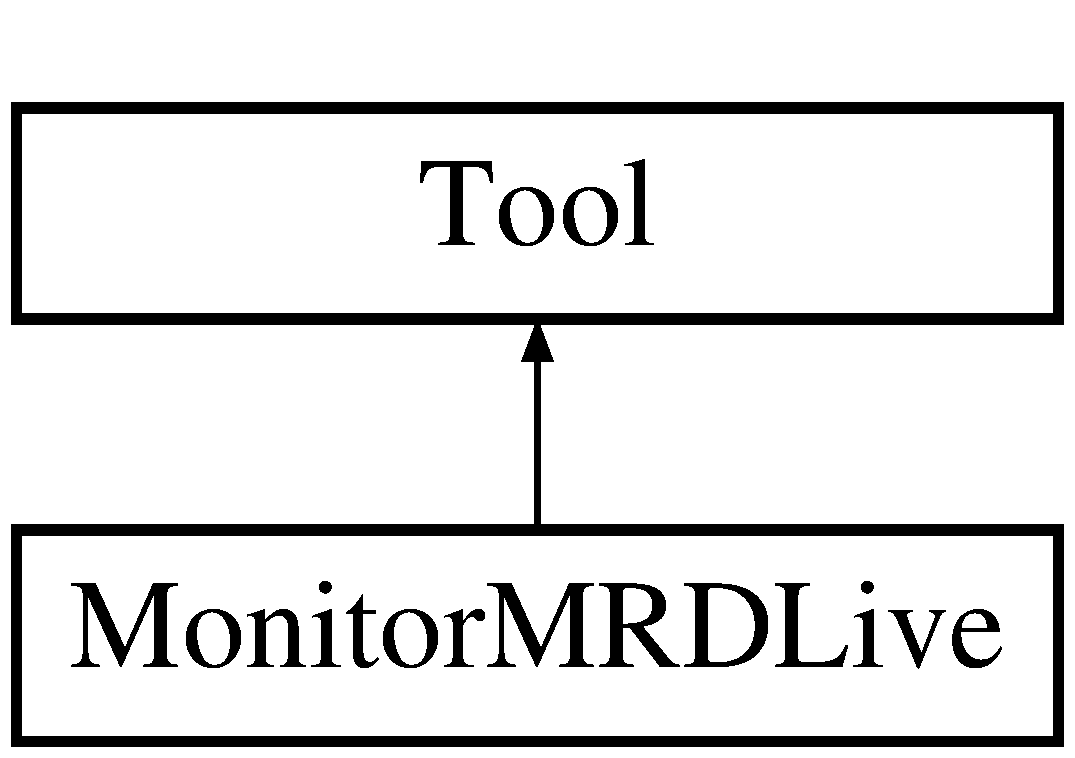
\includegraphics[height=2.000000cm]{classMonitorMRDLive}
\end{center}
\end{figure}
\subsection*{Public Member Functions}
\begin{DoxyCompactItemize}
\item 
\hypertarget{classMonitorMRDLive_a05a63a84f2a7b6e4340d21e2c018a971}{bool {\bfseries Initialise} (std\-::string configfile, \hyperlink{classDataModel}{Data\-Model} \&data)}\label{classMonitorMRDLive_a05a63a84f2a7b6e4340d21e2c018a971}

\item 
\hypertarget{classMonitorMRDLive_a86c7648cc8aad1fb24d86d7f13507128}{bool {\bfseries Execute} ()}\label{classMonitorMRDLive_a86c7648cc8aad1fb24d86d7f13507128}

\item 
\hypertarget{classMonitorMRDLive_ae061bd82e645e7cd1d383badee568d49}{bool {\bfseries Finalise} ()}\label{classMonitorMRDLive_ae061bd82e645e7cd1d383badee568d49}

\item 
\hypertarget{classMonitorMRDLive_a74930d4f7ddc5ff78db48551aa9d6f99}{void {\bfseries M\-R\-D\-T\-D\-C\-Plots} ()}\label{classMonitorMRDLive_a74930d4f7ddc5ff78db48551aa9d6f99}

\end{DoxyCompactItemize}


The documentation for this class was generated from the following files\-:\begin{DoxyCompactItemize}
\item 
User\-Tools/\-Monitor\-M\-R\-D\-Live/Monitor\-M\-R\-D\-Live.\-h\item 
User\-Tools/\-Monitor\-M\-R\-D\-Live/Monitor\-M\-R\-D\-Live.\-cpp\end{DoxyCompactItemize}

\hypertarget{classMonitorMRDTime}{\section{Monitor\-M\-R\-D\-Time Class Reference}
\label{classMonitorMRDTime}\index{Monitor\-M\-R\-D\-Time@{Monitor\-M\-R\-D\-Time}}
}
Inheritance diagram for Monitor\-M\-R\-D\-Time\-:\begin{figure}[H]
\begin{center}
\leavevmode
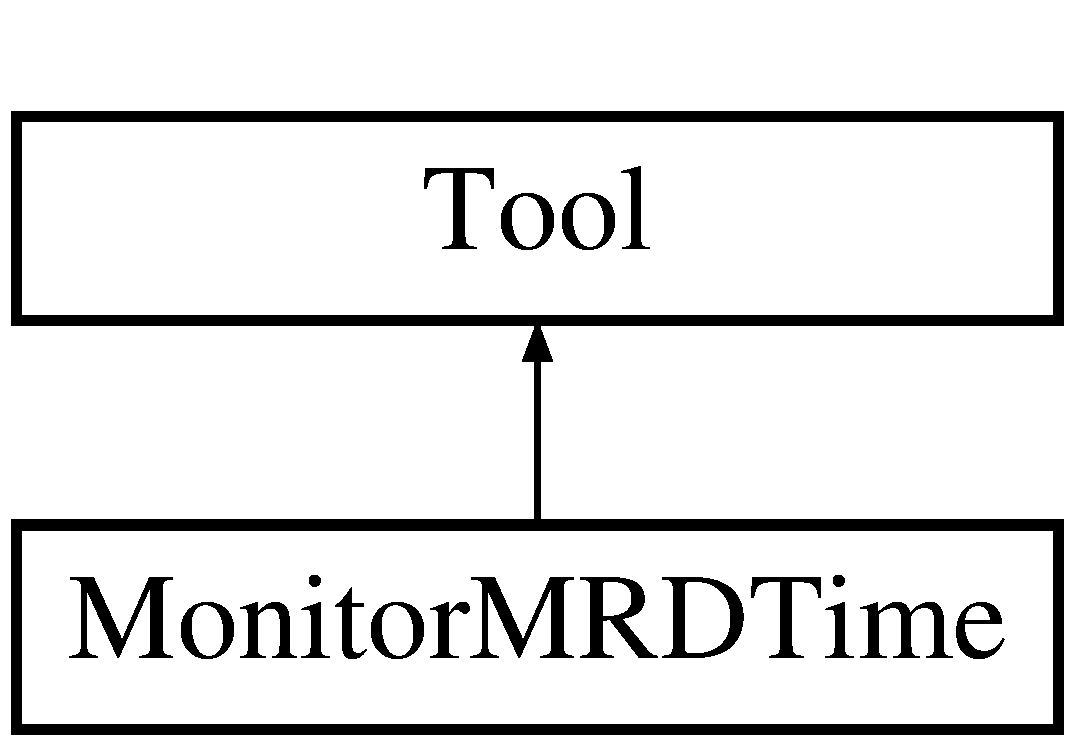
\includegraphics[height=2.000000cm]{classMonitorMRDTime}
\end{center}
\end{figure}
\subsection*{Public Member Functions}
\begin{DoxyCompactItemize}
\item 
\hypertarget{classMonitorMRDTime_a0eb95583c6a147059859b56c0c2687ee}{bool {\bfseries Initialise} (std\-::string configfile, \hyperlink{classDataModel}{Data\-Model} \&data)}\label{classMonitorMRDTime_a0eb95583c6a147059859b56c0c2687ee}

\item 
\hypertarget{classMonitorMRDTime_af322d7679b5199d91caec6ca69226995}{bool {\bfseries Execute} ()}\label{classMonitorMRDTime_af322d7679b5199d91caec6ca69226995}

\item 
\hypertarget{classMonitorMRDTime_ad9b436fb72af740b16468463a50eefe6}{bool {\bfseries Finalise} ()}\label{classMonitorMRDTime_ad9b436fb72af740b16468463a50eefe6}

\item 
\hypertarget{classMonitorMRDTime_affa1155c36568467e553b8e9460ecf8a}{void {\bfseries M\-R\-D\-Time\-Plots} ()}\label{classMonitorMRDTime_affa1155c36568467e553b8e9460ecf8a}

\item 
\hypertarget{classMonitorMRDTime_ad2e2bfb694d2bf99d189f7b4496da16a}{void {\bfseries Update\-Monitor\-Sources} ()}\label{classMonitorMRDTime_ad2e2bfb694d2bf99d189f7b4496da16a}

\item 
\hypertarget{classMonitorMRDTime_ad3380e8bac12fc88745a15dd0b68ed09}{void {\bfseries Fill\-Events} ()}\label{classMonitorMRDTime_ad3380e8bac12fc88745a15dd0b68ed09}

\item 
\hypertarget{classMonitorMRDTime_a3a81ee4967f10349d1f6571f7f4a8696}{void {\bfseries Initialize\-Vectors} ()}\label{classMonitorMRDTime_a3a81ee4967f10349d1f6571f7f4a8696}

\end{DoxyCompactItemize}


The documentation for this class was generated from the following files\-:\begin{DoxyCompactItemize}
\item 
User\-Tools/\-Monitor\-M\-R\-D\-Time/Monitor\-M\-R\-D\-Time.\-h\item 
User\-Tools/\-Monitor\-M\-R\-D\-Time/Monitor\-M\-R\-D\-Time.\-cpp\end{DoxyCompactItemize}

\hypertarget{classMonitorReceive}{
\section{MonitorReceive Class Reference}
\label{classMonitorReceive}\index{MonitorReceive@{MonitorReceive}}
}
\subsection*{Public Member Functions}
\begin{DoxyCompactItemize}
\item 
\hypertarget{classMonitorReceive_a635e0cf91b53352483bb0f30a27c1287}{
bool {\bfseries Initialise} (std::string configfile, \hyperlink{classDataModel}{DataModel} \&data)}
\label{classMonitorReceive_a635e0cf91b53352483bb0f30a27c1287}

\item 
\hypertarget{classMonitorReceive_a316f1f7d2a21f698faa0cb8d0583c49a}{
bool {\bfseries Execute} ()}
\label{classMonitorReceive_a316f1f7d2a21f698faa0cb8d0583c49a}

\item 
\hypertarget{classMonitorReceive_a9f11f11200f7cca1cffc38d9021f831a}{
bool {\bfseries Finalise} ()}
\label{classMonitorReceive_a9f11f11200f7cca1cffc38d9021f831a}

\item 
\hypertarget{classMonitorReceive_a87daa52032531a34d499d4ca510a5627}{
int {\bfseries UpdateMonitorSources} ()}
\label{classMonitorReceive_a87daa52032531a34d499d4ca510a5627}

\end{DoxyCompactItemize}


The documentation for this class was generated from the following files:\begin{DoxyCompactItemize}
\item 
UserTools/MonitorReceive/MonitorReceive.h\item 
UserTools/MonitorReceive/MonitorReceive.cpp\end{DoxyCompactItemize}

\hypertarget{classMonitorSimReceive}{
\section{MonitorSimReceive Class Reference}
\label{classMonitorSimReceive}\index{MonitorSimReceive@{MonitorSimReceive}}
}
\subsection*{Public Member Functions}
\begin{DoxyCompactItemize}
\item 
\hypertarget{classMonitorSimReceive_a3e841c945c5481d97fc82cb4658bdaee}{
bool {\bfseries Initialise} (std::string configfile, \hyperlink{classDataModel}{DataModel} \&data)}
\label{classMonitorSimReceive_a3e841c945c5481d97fc82cb4658bdaee}

\item 
\hypertarget{classMonitorSimReceive_a289c3a6508deff086d9250263cc9981e}{
bool {\bfseries Execute} ()}
\label{classMonitorSimReceive_a289c3a6508deff086d9250263cc9981e}

\item 
\hypertarget{classMonitorSimReceive_afb3fd0f4191c888966b83a0bc8ff032d}{
bool {\bfseries Finalise} ()}
\label{classMonitorSimReceive_afb3fd0f4191c888966b83a0bc8ff032d}

\end{DoxyCompactItemize}


The documentation for this class was generated from the following files:\begin{DoxyCompactItemize}
\item 
UserTools/MonitorSimReceive/MonitorSimReceive.h\item 
UserTools/MonitorSimReceive/MonitorSimReceive.cpp\end{DoxyCompactItemize}

\hypertarget{classMrdDiscriminatorScan}{
\section{MrdDiscriminatorScan Class Reference}
\label{classMrdDiscriminatorScan}\index{MrdDiscriminatorScan@{MrdDiscriminatorScan}}
}
\subsection*{Public Member Functions}
\begin{DoxyCompactItemize}
\item 
\hypertarget{classMrdDiscriminatorScan_abaa4b337b0df9e14620ae6f9b8794b1b}{
bool {\bfseries Initialise} (std::string configfile, \hyperlink{classDataModel}{DataModel} \&data)}
\label{classMrdDiscriminatorScan_abaa4b337b0df9e14620ae6f9b8794b1b}

\item 
\hypertarget{classMrdDiscriminatorScan_a37ebf1bcfc1bdaafe1afddea5bacbd67}{
bool {\bfseries Execute} ()}
\label{classMrdDiscriminatorScan_a37ebf1bcfc1bdaafe1afddea5bacbd67}

\item 
\hypertarget{classMrdDiscriminatorScan_a73fe6971470c0858f87051e2ab853e18}{
bool {\bfseries Finalise} ()}
\label{classMrdDiscriminatorScan_a73fe6971470c0858f87051e2ab853e18}

\end{DoxyCompactItemize}


The documentation for this class was generated from the following files:\begin{DoxyCompactItemize}
\item 
UserTools/MrdDiscriminatorScan/MrdDiscriminatorScan.h\item 
UserTools/MrdDiscriminatorScan/MrdDiscriminatorScan.cpp\end{DoxyCompactItemize}

\hypertarget{classMrdDistributions}{\section{Mrd\-Distributions Class Reference}
\label{classMrdDistributions}\index{Mrd\-Distributions@{Mrd\-Distributions}}
}
Inheritance diagram for Mrd\-Distributions\-:\begin{figure}[H]
\begin{center}
\leavevmode
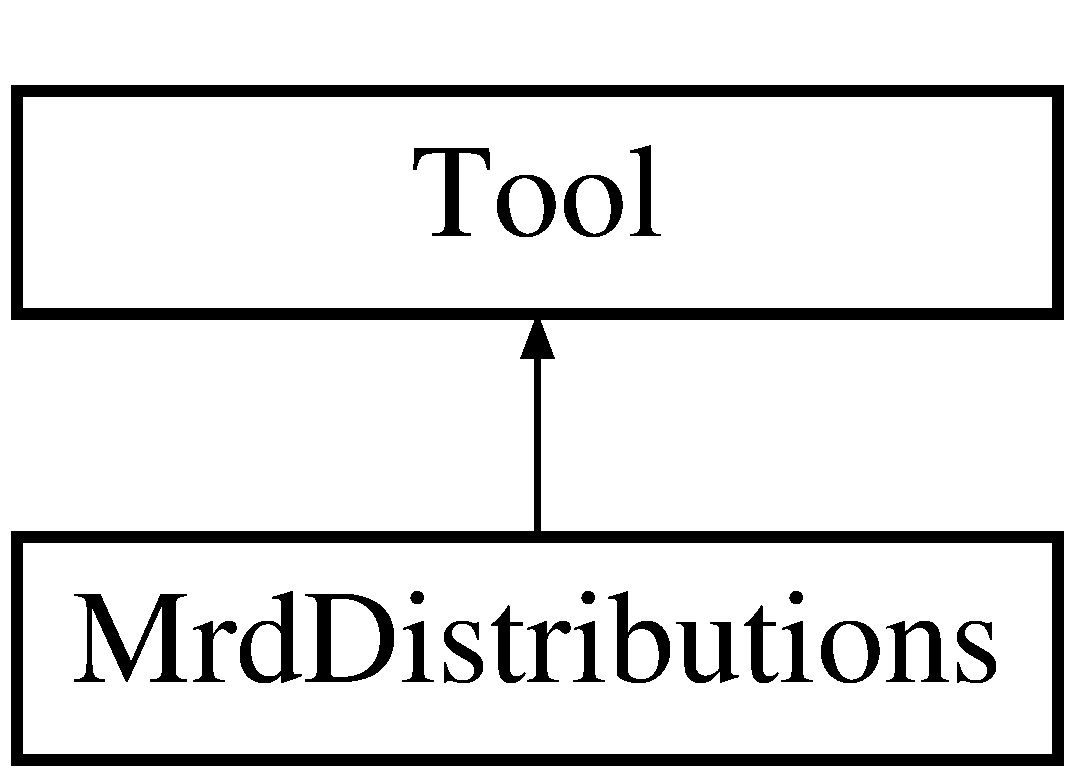
\includegraphics[height=2.000000cm]{classMrdDistributions}
\end{center}
\end{figure}
\subsection*{Public Member Functions}
\begin{DoxyCompactItemize}
\item 
\hypertarget{classMrdDistributions_a0e32e324d6f93d4a45b6b313fc1fb735}{bool {\bfseries Initialise} (std\-::string configfile, \hyperlink{classDataModel}{Data\-Model} \&data)}\label{classMrdDistributions_a0e32e324d6f93d4a45b6b313fc1fb735}

\item 
\hypertarget{classMrdDistributions_a9d925095cb7ff1ede865837076da0b03}{bool {\bfseries Execute} ()}\label{classMrdDistributions_a9d925095cb7ff1ede865837076da0b03}

\item 
\hypertarget{classMrdDistributions_acb7753d5c69220fabc7f93c9bd6f3948}{bool {\bfseries Finalise} ()}\label{classMrdDistributions_acb7753d5c69220fabc7f93c9bd6f3948}

\end{DoxyCompactItemize}
\subsection*{Public Attributes}
\begin{DoxyCompactItemize}
\item 
\hypertarget{classMrdDistributions_a47f2a560f640c946ed721acdf093ab95}{int {\bfseries verbosity} =1}\label{classMrdDistributions_a47f2a560f640c946ed721acdf093ab95}

\item 
\hypertarget{classMrdDistributions_acfa5709e73f4984f9bd4664d11e6ff39}{bool {\bfseries print\-Tracks}}\label{classMrdDistributions_acfa5709e73f4984f9bd4664d11e6ff39}

\item 
\hypertarget{classMrdDistributions_a5b40d02e337e41a40f52f78624bca5d5}{std\-::string {\bfseries plot\-Directory}}\label{classMrdDistributions_a5b40d02e337e41a40f52f78624bca5d5}

\end{DoxyCompactItemize}


The documentation for this class was generated from the following files\-:\begin{DoxyCompactItemize}
\item 
User\-Tools/\-Mrd\-Distributions/Mrd\-Distributions.\-h\item 
User\-Tools/\-Mrd\-Distributions/Mrd\-Distributions.\-cpp\end{DoxyCompactItemize}

\hypertarget{classMrdEfficiency}{
\section{MrdEfficiency Class Reference}
\label{classMrdEfficiency}\index{MrdEfficiency@{MrdEfficiency}}
}
\subsection*{Public Member Functions}
\begin{DoxyCompactItemize}
\item 
\hypertarget{classMrdEfficiency_a08728f36b55f16ae22b542b41af58c30}{
bool {\bfseries Initialise} (std::string configfile, \hyperlink{classDataModel}{DataModel} \&data)}
\label{classMrdEfficiency_a08728f36b55f16ae22b542b41af58c30}

\item 
\hypertarget{classMrdEfficiency_ada02439004731e9ab80cceaf5027ac77}{
bool {\bfseries Execute} ()}
\label{classMrdEfficiency_ada02439004731e9ab80cceaf5027ac77}

\item 
\hypertarget{classMrdEfficiency_a804e18645520f7ede27d4cd7d4a0d666}{
bool {\bfseries Finalise} ()}
\label{classMrdEfficiency_a804e18645520f7ede27d4cd7d4a0d666}

\end{DoxyCompactItemize}
\subsection*{Public Attributes}
\begin{DoxyCompactItemize}
\item 
\hypertarget{classMrdEfficiency_a96c39668e71df6a3e0261bf7aeac9dcb}{
int {\bfseries verbosity} = 1}
\label{classMrdEfficiency_a96c39668e71df6a3e0261bf7aeac9dcb}

\item 
\hypertarget{classMrdEfficiency_af3a7b151047b6f71fcf1333f869c6a72}{
bool {\bfseries drawHistos}}
\label{classMrdEfficiency_af3a7b151047b6f71fcf1333f869c6a72}

\end{DoxyCompactItemize}


The documentation for this class was generated from the following files:\begin{DoxyCompactItemize}
\item 
UserTools/MrdEfficiency/MrdEfficiency.h\item 
UserTools/MrdEfficiency/MrdEfficiency.cpp\end{DoxyCompactItemize}

\hypertarget{classMRDOut}{\section{M\-R\-D\-Out Class Reference}
\label{classMRDOut}\index{M\-R\-D\-Out@{M\-R\-D\-Out}}
}
Inheritance diagram for M\-R\-D\-Out\-:\begin{figure}[H]
\begin{center}
\leavevmode
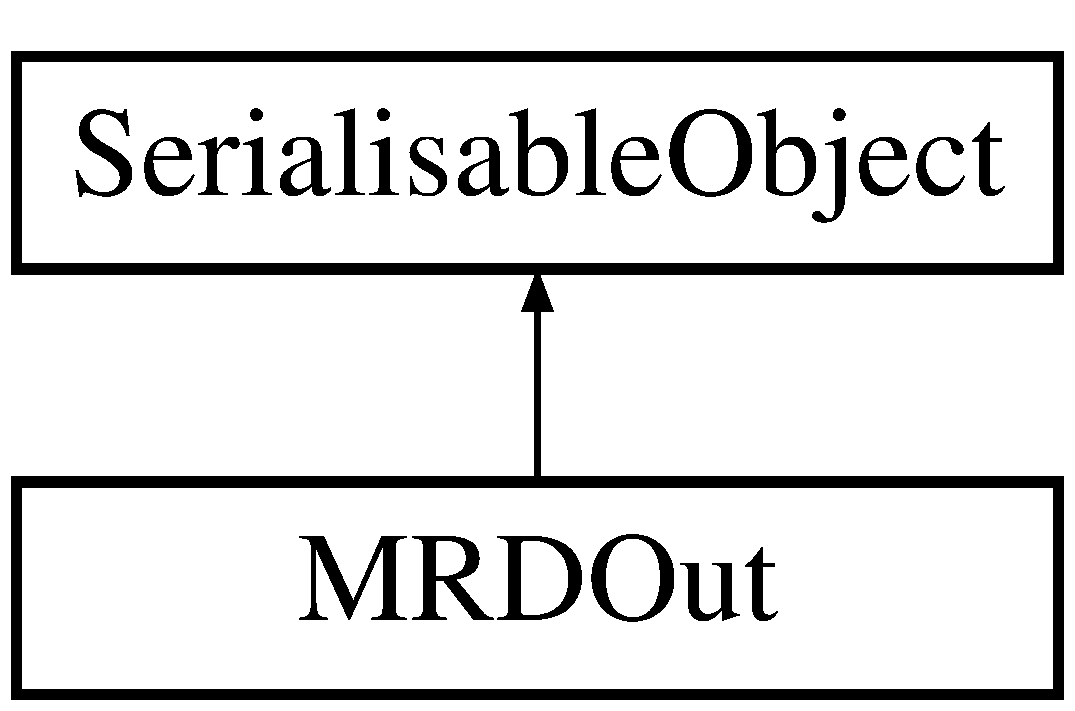
\includegraphics[height=2.000000cm]{classMRDOut}
\end{center}
\end{figure}
\subsection*{Public Member Functions}
\begin{DoxyCompactItemize}
\item 
\hypertarget{classMRDOut_a2c72c51c7288bd4ed73d4c9de0509150}{bool {\bfseries Send} (zmq\-::socket\-\_\-t $\ast$socket)}\label{classMRDOut_a2c72c51c7288bd4ed73d4c9de0509150}

\item 
\hypertarget{classMRDOut_a7e83eb6f2ac421109f907235d4211571}{bool {\bfseries Receive} (zmq\-::socket\-\_\-t $\ast$socket)}\label{classMRDOut_a7e83eb6f2ac421109f907235d4211571}

\item 
\hypertarget{classMRDOut_a956aa4f1b5746c9e12e7b69980d58b62}{bool {\bfseries Print} ()}\label{classMRDOut_a956aa4f1b5746c9e12e7b69980d58b62}

\end{DoxyCompactItemize}
\subsection*{Public Attributes}
\begin{DoxyCompactItemize}
\item 
\hypertarget{classMRDOut_a99fcd630b69a452e867b30bda86b9d6c}{unsigned int {\bfseries Out\-N}}\label{classMRDOut_a99fcd630b69a452e867b30bda86b9d6c}

\item 
\hypertarget{classMRDOut_aefae0cae9b9149247c66fec5140393af}{unsigned int {\bfseries Trigger}}\label{classMRDOut_aefae0cae9b9149247c66fec5140393af}

\item 
\hypertarget{classMRDOut_ae8b80ae7773fb9573a26cf791e18995d}{std\-::vector$<$ unsigned int $>$ {\bfseries Value}}\label{classMRDOut_ae8b80ae7773fb9573a26cf791e18995d}

\item 
\hypertarget{classMRDOut_a03e751accc75934f1ad7926415ce570e}{std\-::vector$<$ unsigned int $>$ {\bfseries Slot}}\label{classMRDOut_a03e751accc75934f1ad7926415ce570e}

\item 
\hypertarget{classMRDOut_a7849667340cd72441d429608ff9b98f9}{std\-::vector$<$ unsigned int $>$ {\bfseries Channel}}\label{classMRDOut_a7849667340cd72441d429608ff9b98f9}

\item 
\hypertarget{classMRDOut_a518db4f65639b83f1e1bcf42f31c1076}{std\-::vector$<$ unsigned int $>$ {\bfseries Crate}}\label{classMRDOut_a518db4f65639b83f1e1bcf42f31c1076}

\item 
\hypertarget{classMRDOut_aa943ba9150d67e2e1758b24324b4ae21}{std\-::vector$<$ std\-::string $>$ {\bfseries Type}}\label{classMRDOut_aa943ba9150d67e2e1758b24324b4ae21}

\item 
\hypertarget{classMRDOut_a1541d7fe5112f7932ec54b285c13eb08}{long {\bfseries Time\-Stamp}}\label{classMRDOut_a1541d7fe5112f7932ec54b285c13eb08}

\end{DoxyCompactItemize}
\subsection*{Friends}
\begin{DoxyCompactItemize}
\item 
\hypertarget{classMRDOut_ac98d07dd8f7b70e16ccb9a01abf56b9c}{class {\bfseries boost\-::serialization\-::access}}\label{classMRDOut_ac98d07dd8f7b70e16ccb9a01abf56b9c}

\end{DoxyCompactItemize}


The documentation for this class was generated from the following files\-:\begin{DoxyCompactItemize}
\item 
Data\-Model/M\-R\-D\-Out.\-h\item 
Data\-Model/M\-R\-D\-Out.\-cpp\end{DoxyCompactItemize}

\hypertarget{classMrdPaddlePlot}{
\section{MrdPaddlePlot Class Reference}
\label{classMrdPaddlePlot}\index{MrdPaddlePlot@{MrdPaddlePlot}}
}
\subsection*{Public Member Functions}
\begin{DoxyCompactItemize}
\item 
\hypertarget{classMrdPaddlePlot_a17a420342671b900521987f9dc070985}{
bool {\bfseries Initialise} (std::string configfile, \hyperlink{classDataModel}{DataModel} \&data)}
\label{classMrdPaddlePlot_a17a420342671b900521987f9dc070985}

\item 
\hypertarget{classMrdPaddlePlot_a655db67bffdbd48ef56a928bb84be1c2}{
bool {\bfseries Execute} ()}
\label{classMrdPaddlePlot_a655db67bffdbd48ef56a928bb84be1c2}

\item 
\hypertarget{classMrdPaddlePlot_ada0f5bfebebcd67b1da1f9db55fb13bc}{
bool {\bfseries Finalise} ()}
\label{classMrdPaddlePlot_ada0f5bfebebcd67b1da1f9db55fb13bc}

\end{DoxyCompactItemize}


The documentation for this class was generated from the following files:\begin{DoxyCompactItemize}
\item 
UserTools/MrdPaddlePlot/MrdPaddlePlot.h\item 
UserTools/MrdPaddlePlot/MrdPaddlePlot.cpp\end{DoxyCompactItemize}

\hypertarget{classMRDPulseFinder}{\section{M\-R\-D\-Pulse\-Finder Class Reference}
\label{classMRDPulseFinder}\index{M\-R\-D\-Pulse\-Finder@{M\-R\-D\-Pulse\-Finder}}
}
Inheritance diagram for M\-R\-D\-Pulse\-Finder\-:\begin{figure}[H]
\begin{center}
\leavevmode
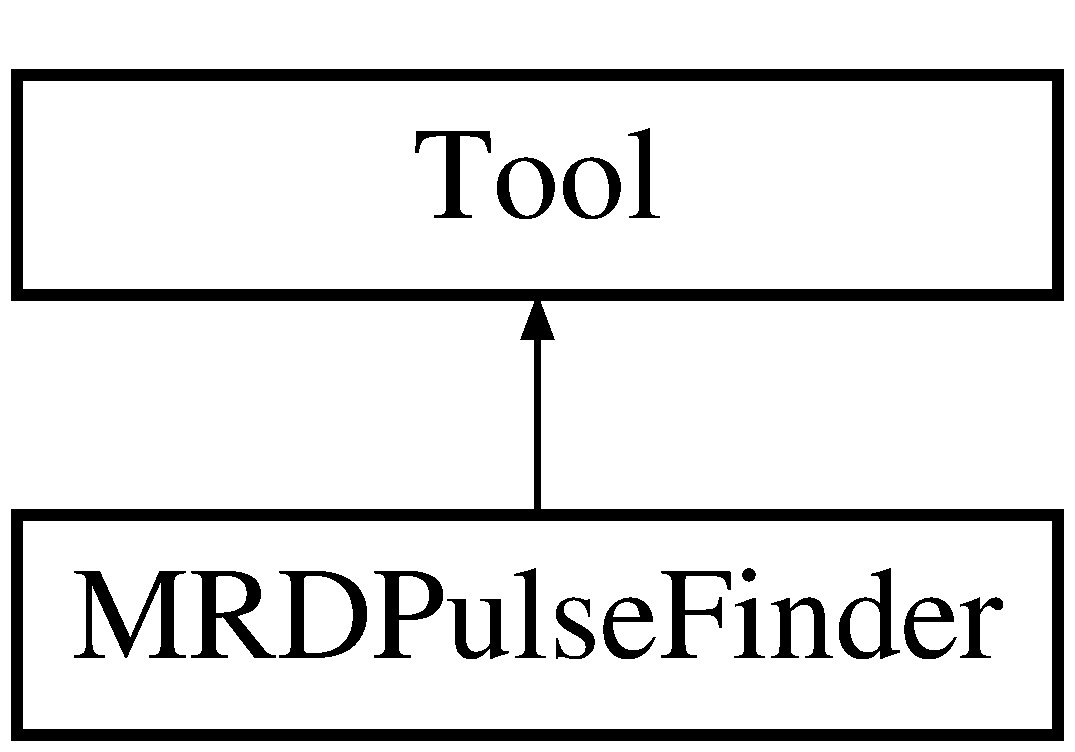
\includegraphics[height=2.000000cm]{classMRDPulseFinder}
\end{center}
\end{figure}
\subsection*{Public Member Functions}
\begin{DoxyCompactItemize}
\item 
\hypertarget{classMRDPulseFinder_ad64f6c541f6d5cc2cb1036a9249837c5}{bool {\bfseries Initialise} (std\-::string configfile, \hyperlink{classDataModel}{Data\-Model} \&data)}\label{classMRDPulseFinder_ad64f6c541f6d5cc2cb1036a9249837c5}

\item 
\hypertarget{classMRDPulseFinder_adff581ca17c601b5ec24a96ad6b85941}{bool {\bfseries Execute} ()}\label{classMRDPulseFinder_adff581ca17c601b5ec24a96ad6b85941}

\item 
\hypertarget{classMRDPulseFinder_a492f228151d4af0a6f07e21ff7e732b0}{bool {\bfseries Finalise} ()}\label{classMRDPulseFinder_a492f228151d4af0a6f07e21ff7e732b0}

\item 
\hypertarget{classMRDPulseFinder_ab82aeb6cbc87a8d0f88252335f261d33}{std\-::vector$<$ \hyperlink{classADCPulse}{A\-D\-C\-Pulse} $>$ {\bfseries Find\-Pulse} (vector$<$ short unsigned int $>$ $\ast$some\-Wave)}\label{classMRDPulseFinder_ab82aeb6cbc87a8d0f88252335f261d33}

\end{DoxyCompactItemize}


The documentation for this class was generated from the following files\-:\begin{DoxyCompactItemize}
\item 
User\-Tools/\-M\-R\-D\-Pulse\-Finder/M\-R\-D\-Pulse\-Finder.\-h\item 
User\-Tools/\-M\-R\-D\-Pulse\-Finder/M\-R\-D\-Pulse\-Finder.\-cpp\end{DoxyCompactItemize}

\hypertarget{classMRDTree}{\section{M\-R\-D\-Tree Class Reference}
\label{classMRDTree}\index{M\-R\-D\-Tree@{M\-R\-D\-Tree}}
}
\subsection*{Public Member Functions}
\begin{DoxyCompactItemize}
\item 
\hypertarget{classMRDTree_aeab336bcc0233f344b19f18cf879d65c}{{\bfseries M\-R\-D\-Tree} (T\-Tree $\ast$tree=0)}\label{classMRDTree_aeab336bcc0233f344b19f18cf879d65c}

\item 
\hypertarget{classMRDTree_acd47df243bbc678e2f06e63c83f2ddf9}{virtual Int\-\_\-t {\bfseries Cut} (Long64\-\_\-t entry)}\label{classMRDTree_acd47df243bbc678e2f06e63c83f2ddf9}

\item 
\hypertarget{classMRDTree_a6257cefb705d4ca769a2848e86a5af65}{virtual Int\-\_\-t {\bfseries Get\-Entry} (Long64\-\_\-t entry)}\label{classMRDTree_a6257cefb705d4ca769a2848e86a5af65}

\item 
\hypertarget{classMRDTree_a2d1700e816c336fd64c219557dce8afc}{virtual Long64\-\_\-t {\bfseries Load\-Tree} (Long64\-\_\-t entry)}\label{classMRDTree_a2d1700e816c336fd64c219557dce8afc}

\item 
\hypertarget{classMRDTree_a7cb7dca1c9b8484a88fe2aa75b326ec5}{virtual void {\bfseries Init} (T\-Tree $\ast$tree)}\label{classMRDTree_a7cb7dca1c9b8484a88fe2aa75b326ec5}

\item 
\hypertarget{classMRDTree_abf8580954488c13d66eed0dde60f96b4}{virtual void {\bfseries Loop} ()}\label{classMRDTree_abf8580954488c13d66eed0dde60f96b4}

\item 
\hypertarget{classMRDTree_a22230efd83c99f624e76b803391aed27}{virtual Bool\-\_\-t {\bfseries Notify} ()}\label{classMRDTree_a22230efd83c99f624e76b803391aed27}

\item 
\hypertarget{classMRDTree_a3f89baaa96b9e85827cc5c1471d0c8c4}{virtual void {\bfseries Show} (Long64\-\_\-t entry=-\/1)}\label{classMRDTree_a3f89baaa96b9e85827cc5c1471d0c8c4}

\end{DoxyCompactItemize}
\subsection*{Public Attributes}
\begin{DoxyCompactItemize}
\item 
\hypertarget{classMRDTree_a73df1663124477ad3347f5a894801079}{T\-Tree $\ast$ {\bfseries f\-Chain}}\label{classMRDTree_a73df1663124477ad3347f5a894801079}

\item 
\hypertarget{classMRDTree_ae34a2e8a27b9deafeb5d28677c4fe090}{Int\-\_\-t \hyperlink{classMRDTree_ae34a2e8a27b9deafeb5d28677c4fe090}{f\-Current}}\label{classMRDTree_ae34a2e8a27b9deafeb5d28677c4fe090}

\begin{DoxyCompactList}\small\item\em pointer to the analyzed T\-Tree or T\-Chain \end{DoxyCompactList}\item 
\hypertarget{classMRDTree_acbb905703b5bd9054df1c685fce4c340}{U\-Int\-\_\-t \hyperlink{classMRDTree_acbb905703b5bd9054df1c685fce4c340}{Trigger}}\label{classMRDTree_acbb905703b5bd9054df1c685fce4c340}

\begin{DoxyCompactList}\small\item\em current Tree number in a T\-Chain \end{DoxyCompactList}\item 
\hypertarget{classMRDTree_ad3a57b2d0d73f13d4fc46d8c3e0c0db8}{U\-Int\-\_\-t {\bfseries Out\-Number}}\label{classMRDTree_ad3a57b2d0d73f13d4fc46d8c3e0c0db8}

\item 
\hypertarget{classMRDTree_aad0e5fe201d44d17706919f231f23b6f}{std\-::vector$<$ std\-::string $>$ $\ast$ {\bfseries Type}}\label{classMRDTree_aad0e5fe201d44d17706919f231f23b6f}

\item 
\hypertarget{classMRDTree_ad30e310155b90d3d76025fba93cb1082}{std\-::vector$<$ unsigned int $>$ $\ast$ {\bfseries Value}}\label{classMRDTree_ad30e310155b90d3d76025fba93cb1082}

\item 
\hypertarget{classMRDTree_ad8a1fdd22f8e261bcc10527ae89aabc3}{std\-::vector$<$ unsigned int $>$ $\ast$ {\bfseries Slot}}\label{classMRDTree_ad8a1fdd22f8e261bcc10527ae89aabc3}

\item 
\hypertarget{classMRDTree_a4275330c81a0e7d017c473e88275dbc7}{std\-::vector$<$ unsigned int $>$ $\ast$ {\bfseries Channel}}\label{classMRDTree_a4275330c81a0e7d017c473e88275dbc7}

\item 
\hypertarget{classMRDTree_abee67bfdf0a6eaf117b85b9b2485612b}{U\-Long64\-\_\-t {\bfseries Time\-Stamp}}\label{classMRDTree_abee67bfdf0a6eaf117b85b9b2485612b}

\item 
\hypertarget{classMRDTree_a555f128842c285877adad7754222feb4}{T\-Branch $\ast$ {\bfseries b\-\_\-\-Trigger}}\label{classMRDTree_a555f128842c285877adad7754222feb4}

\item 
\hypertarget{classMRDTree_abee621e9208bdfcbdb2c2f068e74950d}{T\-Branch $\ast$ {\bfseries b\-\_\-\-Out\-N}}\label{classMRDTree_abee621e9208bdfcbdb2c2f068e74950d}

\item 
\hypertarget{classMRDTree_ae95ac23e8ade856062ca8646cf8b652e}{T\-Branch $\ast$ {\bfseries b\-\_\-\-Type}}\label{classMRDTree_ae95ac23e8ade856062ca8646cf8b652e}

\item 
\hypertarget{classMRDTree_ab5ec56917aad8639be559941dbbbf5f1}{T\-Branch $\ast$ {\bfseries b\-\_\-\-Value}}\label{classMRDTree_ab5ec56917aad8639be559941dbbbf5f1}

\item 
\hypertarget{classMRDTree_a7e22be6df66f4f8da01a836c6ba21251}{T\-Branch $\ast$ {\bfseries b\-\_\-\-Slot}}\label{classMRDTree_a7e22be6df66f4f8da01a836c6ba21251}

\item 
\hypertarget{classMRDTree_a3bb90cc6b5552840b91dfb88ce24d19e}{T\-Branch $\ast$ {\bfseries b\-\_\-\-Channel}}\label{classMRDTree_a3bb90cc6b5552840b91dfb88ce24d19e}

\item 
\hypertarget{classMRDTree_acc8785e5ee2f2702f240bfc1f629decc}{T\-Branch $\ast$ {\bfseries b\-\_\-\-Time\-Stamp}}\label{classMRDTree_acc8785e5ee2f2702f240bfc1f629decc}

\end{DoxyCompactItemize}


The documentation for this class was generated from the following files\-:\begin{DoxyCompactItemize}
\item 
User\-Tools/\-Load\-C\-C\-Data/M\-R\-D\-Tree.\-h\item 
User\-Tools/\-Load\-C\-C\-Data/M\-R\-D\-Tree.\-cpp\end{DoxyCompactItemize}

\hypertarget{classMyTool}{
\section{MyTool Class Reference}
\label{classMyTool}\index{MyTool@{MyTool}}
}


{\ttfamily \#include $<$MyTool.h$>$}\subsection*{Public Member Functions}
\begin{DoxyCompactItemize}
\item 
\hypertarget{classMyTool_ad85b796bdd675ae22e69cf40fe7b6314}{
\hyperlink{classMyTool_ad85b796bdd675ae22e69cf40fe7b6314}{MyTool} ()}
\label{classMyTool_ad85b796bdd675ae22e69cf40fe7b6314}

\begin{DoxyCompactList}\small\item\em Simple constructor. \item\end{DoxyCompactList}\item 
bool \hyperlink{classMyTool_a3bf60061195a18542c4cfb2916b9dad9}{Initialise} (std::string configfile, \hyperlink{classDataModel}{DataModel} \&data)
\begin{DoxyCompactList}\small\item\em Initialise Function for setting up Tool resources. \item\end{DoxyCompactList}\item 
\hypertarget{classMyTool_a0a58122023af90b9200d0e71e89cfb36}{
bool \hyperlink{classMyTool_a0a58122023af90b9200d0e71e89cfb36}{Execute} ()}
\label{classMyTool_a0a58122023af90b9200d0e71e89cfb36}

\begin{DoxyCompactList}\small\item\em Execute function used to perform Tool purpose. \item\end{DoxyCompactList}\item 
\hypertarget{classMyTool_a060ec6356451aa335d0de41093c9992f}{
bool \hyperlink{classMyTool_a060ec6356451aa335d0de41093c9992f}{Finalise} ()}
\label{classMyTool_a060ec6356451aa335d0de41093c9992f}

\begin{DoxyCompactList}\small\item\em Finalise function used to clean up resources. \item\end{DoxyCompactList}\end{DoxyCompactItemize}


\subsection{Detailed Description}
This is a blank template for a Tool used by the script to generate a new custom tool. Please fill out the description and author information.

Author}
B.Richards Date}
2019/05/28 10:44:00 Contact: \href{mailto:b.richards@qmul.ac.uk}{\tt b.richards@qmul.ac.uk} 

\subsection{Member Function Documentation}
\hypertarget{classMyTool_a3bf60061195a18542c4cfb2916b9dad9}{
\index{MyTool@{MyTool}!Initialise@{Initialise}}
\index{Initialise@{Initialise}!MyTool@{MyTool}}
\subsubsection[{Initialise}]{\setlength{\rightskip}{0pt plus 5cm}bool MyTool::Initialise (std::string {\em configfile}, \/  {\bf DataModel} \& {\em data})}}
\label{classMyTool_a3bf60061195a18542c4cfb2916b9dad9}


Initialise Function for setting up Tool resources. 
\begin{DoxyParams}{Parameters}
\item[{\em configfile}]The path and name of the dynamic configuration file to read in. \item[{\em data}]A reference to the transient data class used to pass information between Tools. \end{DoxyParams}


The documentation for this class was generated from the following files:\begin{DoxyCompactItemize}
\item 
UserTools/template/MyTool.h\item 
UserTools/template/MyTool.cpp\end{DoxyCompactItemize}

\hypertarget{structNCVPositionInfo}{
\section{NCVPositionInfo Struct Reference}
\label{structNCVPositionInfo}\index{NCVPositionInfo@{NCVPositionInfo}}
}
\subsection*{Public Attributes}
\begin{DoxyCompactItemize}
\item 
\hypertarget{structNCVPositionInfo_ace4afc2346cc29522e1732f9f41de8dd}{
double {\bfseries total\_\-POT} = 0.}
\label{structNCVPositionInfo_ace4afc2346cc29522e1732f9f41de8dd}

\item 
\hypertarget{structNCVPositionInfo_a813f7edef83ad94a009257ece03392dd}{
uint64\_\-t {\bfseries num\_\-beam\_\-spills} = 0ull}
\label{structNCVPositionInfo_a813f7edef83ad94a009257ece03392dd}

\item 
\hypertarget{structNCVPositionInfo_aa9303f33637e7e3f3a47dbc1ec915e97}{
uint64\_\-t {\bfseries num\_\-source\_\-triggers} = 0ull}
\label{structNCVPositionInfo_aa9303f33637e7e3f3a47dbc1ec915e97}

\item 
\hypertarget{structNCVPositionInfo_a5e5afcbdc00981d16728e325c0a8eca9}{
uint64\_\-t {\bfseries num\_\-cosmic\_\-triggers} = 0ull}
\label{structNCVPositionInfo_a5e5afcbdc00981d16728e325c0a8eca9}

\item 
\hypertarget{structNCVPositionInfo_ac4c3befd94418e04f02d2549569bd5eb}{
uint64\_\-t {\bfseries num\_\-soft\_\-triggers} = 0ull}
\label{structNCVPositionInfo_ac4c3befd94418e04f02d2549569bd5eb}

\end{DoxyCompactItemize}


The documentation for this struct was generated from the following file:\begin{DoxyCompactItemize}
\item 
UserTools/PhaseITreeMaker/PhaseITreeMaker.h\end{DoxyCompactItemize}

\hypertarget{classNeutronStudyPMCS}{\section{Neutron\-Study\-P\-M\-C\-S Class Reference}
\label{classNeutronStudyPMCS}\index{Neutron\-Study\-P\-M\-C\-S@{Neutron\-Study\-P\-M\-C\-S}}
}
Inheritance diagram for Neutron\-Study\-P\-M\-C\-S\-:\begin{figure}[H]
\begin{center}
\leavevmode
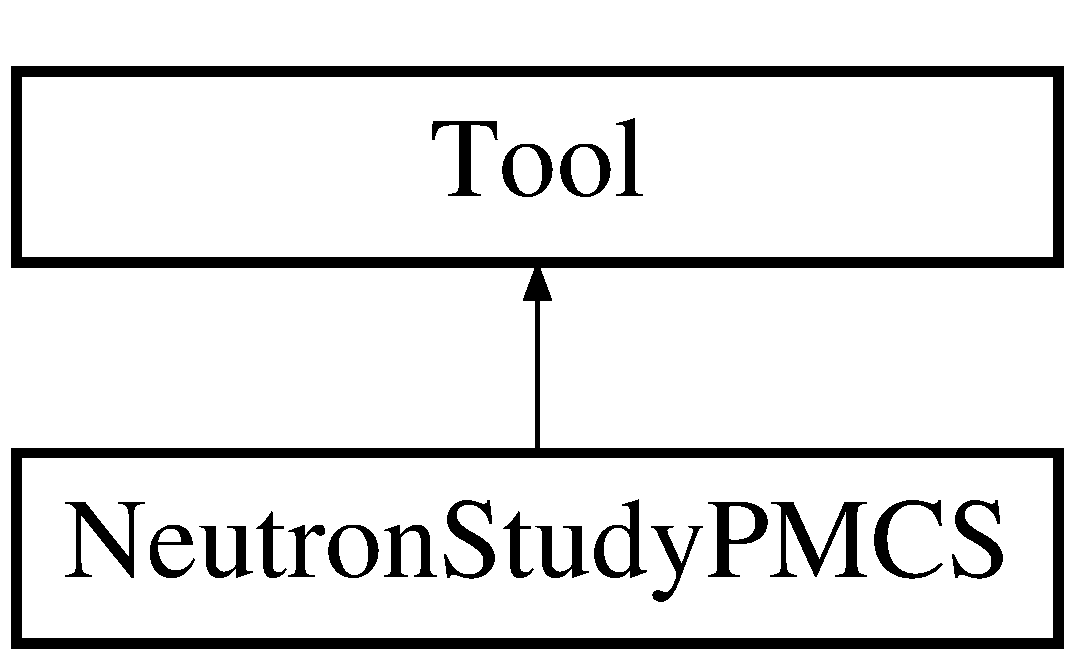
\includegraphics[height=2.000000cm]{classNeutronStudyPMCS}
\end{center}
\end{figure}
\subsection*{Public Member Functions}
\begin{DoxyCompactItemize}
\item 
\hypertarget{classNeutronStudyPMCS_a044b07d39e07fbac5764b8788f11a3ec}{bool {\bfseries Initialise} (std\-::string configfile, \hyperlink{classDataModel}{Data\-Model} \&data)}\label{classNeutronStudyPMCS_a044b07d39e07fbac5764b8788f11a3ec}

\item 
\hypertarget{classNeutronStudyPMCS_a1cc06822548c3febc0708db5b59c343b}{bool {\bfseries Execute} ()}\label{classNeutronStudyPMCS_a1cc06822548c3febc0708db5b59c343b}

\item 
\hypertarget{classNeutronStudyPMCS_aa4e1c744c42f16c63b4ddefefda81922}{bool {\bfseries Finalise} ()}\label{classNeutronStudyPMCS_aa4e1c744c42f16c63b4ddefefda81922}

\item 
\hypertarget{classNeutronStudyPMCS_acdaa5568f44221b53168e490969393bf}{double {\bfseries nu\-E\-Efficiency} (double nu\-E)}\label{classNeutronStudyPMCS_acdaa5568f44221b53168e490969393bf}

\item 
\hypertarget{classNeutronStudyPMCS_aefc2ab996c1c513c0f032931f3f67e7e}{double {\bfseries Muon\-Efficiency} (double mu\-\_\-\-E, double mu\-\_\-angle)}\label{classNeutronStudyPMCS_aefc2ab996c1c513c0f032931f3f67e7e}

\item 
\hypertarget{classNeutronStudyPMCS_ad0cfe53c957f4a47fbe60f7bc390e32b}{double {\bfseries Pion\-Inefficiency} (double pi\-\_\-\-E, double pi\-\_\-angle)}\label{classNeutronStudyPMCS_ad0cfe53c957f4a47fbe60f7bc390e32b}

\item 
\hypertarget{classNeutronStudyPMCS_aa55a9508e67f6c758b1e7ecb7ff87a74}{double {\bfseries Mu\-Esmear} (double mu\-\_\-\-E, double Eres)}\label{classNeutronStudyPMCS_aa55a9508e67f6c758b1e7ecb7ff87a74}

\item 
\hypertarget{classNeutronStudyPMCS_ad04d525456090178ee877757d120993a}{double {\bfseries Mu\-Anglesmear} (double mu\-\_\-px, double mu\-\_\-py, double mu\-\_\-pz, double angsmear)}\label{classNeutronStudyPMCS_ad04d525456090178ee877757d120993a}

\item 
\hypertarget{classNeutronStudyPMCS_a87bfadcdde1434cd4aaa66ff9968a121}{double {\bfseries Reco\-E} (double mu\-\_\-\-E, double mu\-\_\-angle)}\label{classNeutronStudyPMCS_a87bfadcdde1434cd4aaa66ff9968a121}

\item 
\hypertarget{classNeutronStudyPMCS_aadac422e432f47ceae16a87a8d2679bb}{int {\bfseries Detected\-Neutrons} (int totneut)}\label{classNeutronStudyPMCS_aadac422e432f47ceae16a87a8d2679bb}

\item 
\hypertarget{classNeutronStudyPMCS_a73c188dfa2d0465729cc3e7c2d68a1bd}{int {\bfseries Bkg\-Neutrons} (double prob)}\label{classNeutronStudyPMCS_a73c188dfa2d0465729cc3e7c2d68a1bd}

\end{DoxyCompactItemize}


The documentation for this class was generated from the following files\-:\begin{DoxyCompactItemize}
\item 
User\-Tools/\-Neutron\-Study\-P\-M\-C\-S/Neutron\-Study\-P\-M\-C\-S.\-h\item 
User\-Tools/\-Neutron\-Study\-P\-M\-C\-S/Neutron\-Study\-P\-M\-C\-S.\-cpp\end{DoxyCompactItemize}

\hypertarget{classNeutronStudyReadSandbox}{\section{Neutron\-Study\-Read\-Sandbox Class Reference}
\label{classNeutronStudyReadSandbox}\index{Neutron\-Study\-Read\-Sandbox@{Neutron\-Study\-Read\-Sandbox}}
}
Inheritance diagram for Neutron\-Study\-Read\-Sandbox\-:\begin{figure}[H]
\begin{center}
\leavevmode
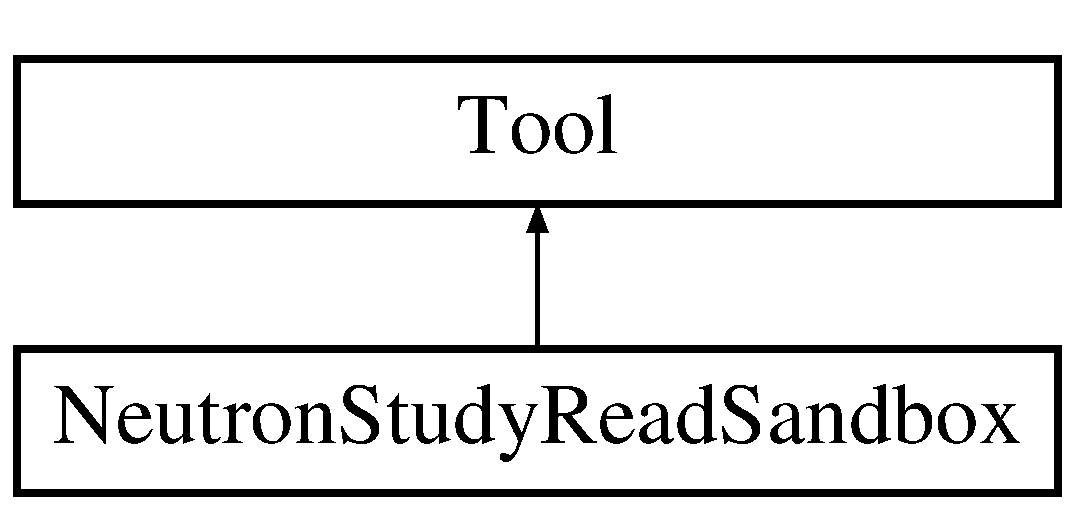
\includegraphics[height=2.000000cm]{classNeutronStudyReadSandbox}
\end{center}
\end{figure}
\subsection*{Public Member Functions}
\begin{DoxyCompactItemize}
\item 
\hypertarget{classNeutronStudyReadSandbox_a9e73e205358244c86e066bb28266066f}{bool {\bfseries Initialise} (std\-::string configfile, \hyperlink{classDataModel}{Data\-Model} \&data)}\label{classNeutronStudyReadSandbox_a9e73e205358244c86e066bb28266066f}

\item 
\hypertarget{classNeutronStudyReadSandbox_a580157d5a29b14c99e698f0919b65049}{bool {\bfseries Execute} ()}\label{classNeutronStudyReadSandbox_a580157d5a29b14c99e698f0919b65049}

\item 
\hypertarget{classNeutronStudyReadSandbox_af76eafb91eaf9270a9423e15026d8e20}{bool {\bfseries Finalise} ()}\label{classNeutronStudyReadSandbox_af76eafb91eaf9270a9423e15026d8e20}

\end{DoxyCompactItemize}


The documentation for this class was generated from the following files\-:\begin{DoxyCompactItemize}
\item 
User\-Tools/\-Neutron\-Study\-Read\-Sandbox/Neutron\-Study\-Read\-Sandbox.\-h\item 
User\-Tools/\-Neutron\-Study\-Read\-Sandbox/Neutron\-Study\-Read\-Sandbox.\-cpp\end{DoxyCompactItemize}

\hypertarget{classNeutronStudyWriteTree}{
\section{NeutronStudyWriteTree Class Reference}
\label{classNeutronStudyWriteTree}\index{NeutronStudyWriteTree@{NeutronStudyWriteTree}}
}
\subsection*{Public Member Functions}
\begin{DoxyCompactItemize}
\item 
\hypertarget{classNeutronStudyWriteTree_a6fa5e7ec01a703b7589583e8c5af744d}{
bool {\bfseries Initialise} (std::string configfile, \hyperlink{classDataModel}{DataModel} \&data)}
\label{classNeutronStudyWriteTree_a6fa5e7ec01a703b7589583e8c5af744d}

\item 
\hypertarget{classNeutronStudyWriteTree_a9e89fb86ad252f39f5f173e0bd8f3528}{
bool {\bfseries Execute} ()}
\label{classNeutronStudyWriteTree_a9e89fb86ad252f39f5f173e0bd8f3528}

\item 
\hypertarget{classNeutronStudyWriteTree_ad11e2482834166c4630ddf4cd8fd6d38}{
bool {\bfseries Finalise} ()}
\label{classNeutronStudyWriteTree_ad11e2482834166c4630ddf4cd8fd6d38}

\end{DoxyCompactItemize}


The documentation for this class was generated from the following files:\begin{DoxyCompactItemize}
\item 
UserTools/NeutronStudyWriteTree/NeutronStudyWriteTree.h\item 
UserTools/NeutronStudyWriteTree/NeutronStudyWriteTree.cpp\end{DoxyCompactItemize}

\hypertarget{classParameters}{
\section{Parameters Class Reference}
\label{classParameters}\index{Parameters@{Parameters}}
}
\subsection*{Public Member Functions}
\begin{DoxyCompactItemize}
\item 
\hypertarget{classParameters_ad51d449c4d2963bef72fde2308966d8b}{
void {\bfseries RunPrintParameters} ()}
\label{classParameters_ad51d449c4d2963bef72fde2308966d8b}

\item 
\hypertarget{classParameters_a08f0965d2fe93066d0c550f08716829d}{
void {\bfseries SetSimpleTimeResolution} ()}
\label{classParameters_a08f0965d2fe93066d0c550f08716829d}

\item 
\hypertarget{classParameters_ac1d25752b880deb537aa4344b40dca5e}{
bool {\bfseries SimpleTimeResolution} ()}
\label{classParameters_ac1d25752b880deb537aa4344b40dca5e}

\item 
\hypertarget{classParameters_ac11f733ad0fa1552e523972433cbe0d1}{
void {\bfseries SetSimpleTimeSlew} ()}
\label{classParameters_ac11f733ad0fa1552e523972433cbe0d1}

\item 
\hypertarget{classParameters_aff94a6d602c527a3690cd1e79970b00b}{
bool {\bfseries SimpleTimeSlew} ()}
\label{classParameters_aff94a6d602c527a3690cd1e79970b00b}

\item 
\hypertarget{classParameters_a7c15c7be2a780eb1110ee3767eea4555}{
void {\bfseries SetSimpleRefractiveIndex} ()}
\label{classParameters_a7c15c7be2a780eb1110ee3767eea4555}

\item 
\hypertarget{classParameters_a66a9a682eff6bf1f55aae967da3f7beb}{
bool {\bfseries SimpleRefractiveIndex} ()}
\label{classParameters_a66a9a682eff6bf1f55aae967da3f7beb}

\item 
\hypertarget{classParameters_a593ddf265554ac4fb05f86d9ac82bc7a}{
double {\bfseries GetCherenkovAngle} ()}
\label{classParameters_a593ddf265554ac4fb05f86d9ac82bc7a}

\item 
\hypertarget{classParameters_a754e96439c2c90e10337737055fbae8a}{
double {\bfseries GetTimeResolution} (double Q)}
\label{classParameters_a754e96439c2c90e10337737055fbae8a}

\item 
\hypertarget{classParameters_a9923cf8f51802396ddb7deea4329104d}{
double {\bfseries GetTimeResolution} (int DigitType)}
\label{classParameters_a9923cf8f51802396ddb7deea4329104d}

\item 
\hypertarget{classParameters_ae4c02a415ab0ac0290aa4e5b937130f0}{
double {\bfseries GetTimeResolution} (int DigitType, double Q)}
\label{classParameters_ae4c02a415ab0ac0290aa4e5b937130f0}

\item 
\hypertarget{classParameters_a86cfc7d93752dcd1549935fd4c3ef3be}{
double {\bfseries GetPositionResolution} (int DigitType)}
\label{classParameters_a86cfc7d93752dcd1549935fd4c3ef3be}

\item 
\hypertarget{classParameters_a59b9a4a70d5b3a1806e85409ab59fa06}{
double {\bfseries GetTimeSlew} (double Q)}
\label{classParameters_a59b9a4a70d5b3a1806e85409ab59fa06}

\item 
\hypertarget{classParameters_af68d5a1e8b879d8bd3e40619dbdcad17}{
double {\bfseries GetRefractiveIndex} (double r)}
\label{classParameters_af68d5a1e8b879d8bd3e40619dbdcad17}

\item 
\hypertarget{classParameters_a87885862d3dec908cc69488f9a5ba414}{
int {\bfseries GetSeedDigitType} ()}
\label{classParameters_a87885862d3dec908cc69488f9a5ba414}

\item 
\hypertarget{classParameters_a7af86855d446b0d87990a5ee0bec878d}{
std::string {\bfseries GetConfigurationType} ()}
\label{classParameters_a7af86855d446b0d87990a5ee0bec878d}

\item 
\hypertarget{classParameters_a5dc92999b540e49c64c0d9cf989a0a57}{
double {\bfseries GetSimpleTimeResolution} (double Q)}
\label{classParameters_a5dc92999b540e49c64c0d9cf989a0a57}

\item 
\hypertarget{classParameters_a9171fa97b63774daaaab2ba0a4534846}{
double {\bfseries GetSimpleTimeSlew} ()}
\label{classParameters_a9171fa97b63774daaaab2ba0a4534846}

\item 
\hypertarget{classParameters_a30c2cab5179a2beb2ad468f8de91b3c0}{
double {\bfseries GetSimpleRefractiveIndex} ()}
\label{classParameters_a30c2cab5179a2beb2ad468f8de91b3c0}

\end{DoxyCompactItemize}
\subsection*{Static Public Member Functions}
\begin{DoxyCompactItemize}
\item 
\hypertarget{classParameters_a116c287173521b39aaef6d9ae2f1168f}{
static \hyperlink{classParameters}{Parameters} $\ast$ {\bfseries Instance} ()}
\label{classParameters_a116c287173521b39aaef6d9ae2f1168f}

\item 
\hypertarget{classParameters_aceaf40bdd65a08ebfa507ae05f1a7633}{
static void {\bfseries UseSimpleParameters} ()}
\label{classParameters_aceaf40bdd65a08ebfa507ae05f1a7633}

\item 
\hypertarget{classParameters_aa0d5f324fe5c3e1418ece481c11bc3eb}{
static void {\bfseries UseSimpleTimeResolution} ()}
\label{classParameters_aa0d5f324fe5c3e1418ece481c11bc3eb}

\item 
\hypertarget{classParameters_a3c61940ae61811d6ca29490978a2a62b}{
static void {\bfseries UseSimpleTimeSlew} ()}
\label{classParameters_a3c61940ae61811d6ca29490978a2a62b}

\item 
\hypertarget{classParameters_a9a9a5eeb5df6d4e60fd9b530fc423aa5}{
static void {\bfseries UseSimpleRefractiveIndex} ()}
\label{classParameters_a9a9a5eeb5df6d4e60fd9b530fc423aa5}

\item 
\hypertarget{classParameters_acc1d5f6429ddb3ab5bd8b0573f049f19}{
static double {\bfseries SpeedOfLight} ()}
\label{classParameters_acc1d5f6429ddb3ab5bd8b0573f049f19}

\item 
\hypertarget{classParameters_a0f0992984d8940acce2ad65a4e5be0b4}{
static double {\bfseries CherenkovAngle} ()}
\label{classParameters_a0f0992984d8940acce2ad65a4e5be0b4}

\item 
\hypertarget{classParameters_a31bf30badb89527522d36cd509a44ec3}{
static double {\bfseries Index0} ()}
\label{classParameters_a31bf30badb89527522d36cd509a44ec3}

\item 
\hypertarget{classParameters_ad26c530d23bc0f13afb8ed08c060fe13}{
static double {\bfseries TimeResolution} (double Q)}
\label{classParameters_ad26c530d23bc0f13afb8ed08c060fe13}

\item 
\hypertarget{classParameters_a4a79efe76cdd7f76870e71936f3bc006}{
static double {\bfseries TimeResolution} (int DigitType)}
\label{classParameters_a4a79efe76cdd7f76870e71936f3bc006}

\item 
\hypertarget{classParameters_a96b3aa83418fef97061a4e7647343989}{
static double {\bfseries TimeResolution} (int DigitType, double Q)}
\label{classParameters_a96b3aa83418fef97061a4e7647343989}

\item 
\hypertarget{classParameters_ac6f65898fef36531ed9fddf04708b577}{
static double {\bfseries PositionResolution} (int DigitType)}
\label{classParameters_ac6f65898fef36531ed9fddf04708b577}

\item 
\hypertarget{classParameters_aecd4991eb52328637dc849c04e254d0f}{
static double {\bfseries TimeSlew} (double Q)}
\label{classParameters_aecd4991eb52328637dc849c04e254d0f}

\item 
\hypertarget{classParameters_ad4f2815a0e46ecdd573fda40d3ef4710}{
static double {\bfseries RefractiveIndex} (double r)}
\label{classParameters_ad4f2815a0e46ecdd573fda40d3ef4710}

\item 
\hypertarget{classParameters_a6feb77688ce48e84f5450332552c348b}{
static double {\bfseries ThetaC} ()}
\label{classParameters_a6feb77688ce48e84f5450332552c348b}

\item 
\hypertarget{classParameters_a87680cdd958e703d73854700fb675a73}{
static double {\bfseries CosThetaC} ()}
\label{classParameters_a87680cdd958e703d73854700fb675a73}

\item 
\hypertarget{classParameters_aa5c5a5e9cfbc338de62e659de1950543}{
static double {\bfseries TimeNoiseRate} ()}
\label{classParameters_aa5c5a5e9cfbc338de62e659de1950543}

\item 
\hypertarget{classParameters_a5c88994da52292b5474849482a524a72}{
static int {\bfseries SeedDigitType} ()}
\label{classParameters_a5c88994da52292b5474849482a524a72}

\item 
\hypertarget{classParameters_a07f0ae805cea2c93da65f5f0e9e7fc21}{
static void {\bfseries PrintParameters} ()}
\label{classParameters_a07f0ae805cea2c93da65f5f0e9e7fc21}

\end{DoxyCompactItemize}
\subsection*{Public Attributes}
\begin{DoxyCompactItemize}
\item 
\hypertarget{classParameters_a0ab2806085b853d149fd6e4c8e569cca}{
double {\bfseries fSpeedOfLight}}
\label{classParameters_a0ab2806085b853d149fd6e4c8e569cca}

\item 
\hypertarget{classParameters_ab8ef3df2fb41ab745ff7647dbc8cc50b}{
double {\bfseries fCherenkovAngle}}
\label{classParameters_ab8ef3df2fb41ab745ff7647dbc8cc50b}

\item 
\hypertarget{classParameters_a71d8363c51b45b3eea2845316a8a4f5d}{
double {\bfseries fRefractiveIndex}}
\label{classParameters_a71d8363c51b45b3eea2845316a8a4f5d}

\item 
\hypertarget{classParameters_ad90255179abb7853ac6d16e5905aa6c6}{
double {\bfseries fTimeNoiseRate}}
\label{classParameters_ad90255179abb7853ac6d16e5905aa6c6}

\item 
\hypertarget{classParameters_ace595d49d4d72a00af0becfcb7c92dad}{
double {\bfseries fPMTTimeResolution}}
\label{classParameters_ace595d49d4d72a00af0becfcb7c92dad}

\item 
\hypertarget{classParameters_a94b1d9e403f02af9ba58763803eef51e}{
double {\bfseries fPMTPositionResolution}}
\label{classParameters_a94b1d9e403f02af9ba58763803eef51e}

\item 
\hypertarget{classParameters_a92dbf523ca3a928c72e18cff5e93f4cb}{
double {\bfseries fLAPPDTimeResolution}}
\label{classParameters_a92dbf523ca3a928c72e18cff5e93f4cb}

\item 
\hypertarget{classParameters_a32904c328c259d8eb7760799d2209cee}{
double {\bfseries fLAPPDPositionResolution}}
\label{classParameters_a32904c328c259d8eb7760799d2209cee}

\item 
\hypertarget{classParameters_a681104d5b6cc6f589095f5759b7e0480}{
int {\bfseries fSeedDigitType}}
\label{classParameters_a681104d5b6cc6f589095f5759b7e0480}

\item 
\hypertarget{classParameters_aed4dffbeb510be19702f836a75cecc7f}{
std::string {\bfseries fConfigurationType}}
\label{classParameters_aed4dffbeb510be19702f836a75cecc7f}

\item 
\hypertarget{classParameters_a2e0a3f1bbb8ffa7e40f84d09452f1f41}{
std::vector$<$ int $>$ {\bfseries fLappdId}}
\label{classParameters_a2e0a3f1bbb8ffa7e40f84d09452f1f41}

\end{DoxyCompactItemize}


The documentation for this class was generated from the following files:\begin{DoxyCompactItemize}
\item 
DataModel/Parameters.h\item 
DataModel/Parameters.cpp\end{DoxyCompactItemize}

\hypertarget{classParticle}{
\section{Particle Class Reference}
\label{classParticle}\index{Particle@{Particle}}
}
Inheritance diagram for Particle::\begin{figure}[H]
\begin{center}
\leavevmode
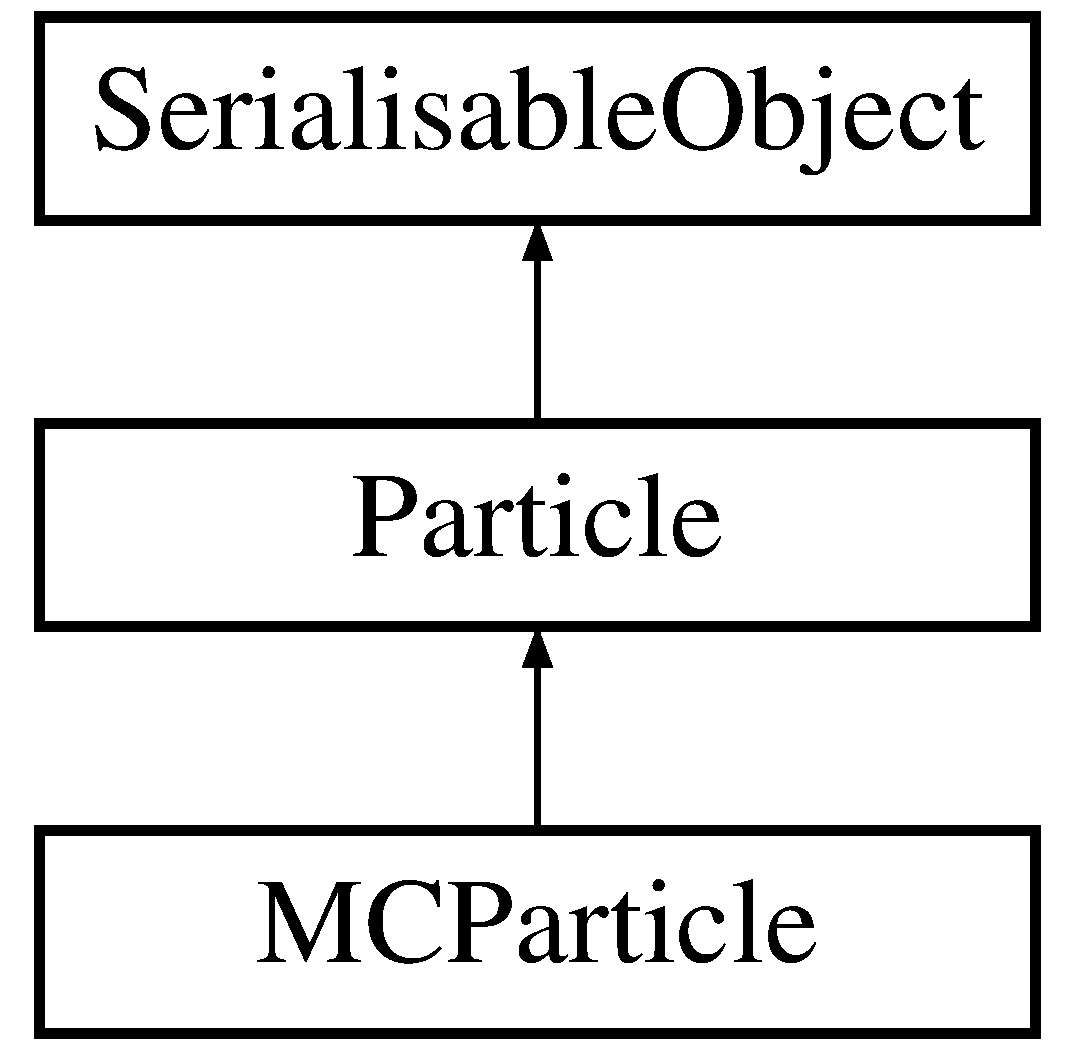
\includegraphics[height=3cm]{classParticle}
\end{center}
\end{figure}
\subsection*{Public Member Functions}
\begin{DoxyCompactItemize}
\item 
\hypertarget{classParticle_a10c8ee36554a8ad1d3f910537a88567a}{
{\bfseries Particle} (int pdg, double sttE, double stpE, \hyperlink{classPosition}{Position} sttpos, \hyperlink{classPosition}{Position} stppos, double sttt, double stpt, \hyperlink{classDirection}{Direction} startdir, double len, tracktype tracktypein)}
\label{classParticle_a10c8ee36554a8ad1d3f910537a88567a}

\item 
\hypertarget{classParticle_a1032e7cf325e073f2bbc7a0447c17780}{
void {\bfseries SetPdgCode} (int code)}
\label{classParticle_a1032e7cf325e073f2bbc7a0447c17780}

\item 
\hypertarget{classParticle_a83b748ccb2402b630ebc2be12b697383}{
void {\bfseries SetStartEnergy} (double E)}
\label{classParticle_a83b748ccb2402b630ebc2be12b697383}

\item 
\hypertarget{classParticle_a427b73c000394c699f92bee299208f84}{
void {\bfseries SetStopEnergy} (double E)}
\label{classParticle_a427b73c000394c699f92bee299208f84}

\item 
\hypertarget{classParticle_a44c601a3c061fd42a7be111ce47c1946}{
void {\bfseries SetStartVertex} (\hyperlink{classPosition}{Position} pos)}
\label{classParticle_a44c601a3c061fd42a7be111ce47c1946}

\item 
\hypertarget{classParticle_a534cc15b476cd65617c02711b6082a5a}{
void {\bfseries SetStopVertex} (\hyperlink{classPosition}{Position} pos)}
\label{classParticle_a534cc15b476cd65617c02711b6082a5a}

\item 
\hypertarget{classParticle_a71be9f9aef04cb704ab99df9da267b04}{
void {\bfseries SetStartTime} (double stime)}
\label{classParticle_a71be9f9aef04cb704ab99df9da267b04}

\item 
\hypertarget{classParticle_a02576e01713e80369ff7c7aa7ead331d}{
void {\bfseries SetStopTime} (double stime)}
\label{classParticle_a02576e01713e80369ff7c7aa7ead331d}

\item 
\hypertarget{classParticle_ae47d25ec4e0d67cada6f4ebcb7696255}{
void {\bfseries SetstartDirection} (\hyperlink{classDirection}{Direction} dir)}
\label{classParticle_ae47d25ec4e0d67cada6f4ebcb7696255}

\item 
\hypertarget{classParticle_a09fe260918298982e88d085bc02e367b}{
void {\bfseries SetTrackLength} (double len)}
\label{classParticle_a09fe260918298982e88d085bc02e367b}

\item 
\hypertarget{classParticle_a9ab8ff63c2cdd3c634ef03d9a96d05a0}{
void {\bfseries SetTrackStartStopType} (tracktype tracktypein)}
\label{classParticle_a9ab8ff63c2cdd3c634ef03d9a96d05a0}

\item 
\hypertarget{classParticle_ac4aef1157eca6d3e79adabca530b3b30}{
int {\bfseries GetPdgCode} ()}
\label{classParticle_ac4aef1157eca6d3e79adabca530b3b30}

\item 
\hypertarget{classParticle_aa8a441034e0e6671e5e9067b2feb2532}{
double {\bfseries GetStartEnergy} ()}
\label{classParticle_aa8a441034e0e6671e5e9067b2feb2532}

\item 
\hypertarget{classParticle_aedd7d21b6a8008a093499d604c72c8b2}{
double {\bfseries GetStopEnergy} ()}
\label{classParticle_aedd7d21b6a8008a093499d604c72c8b2}

\item 
\hypertarget{classParticle_a80f0b4c9a5dbca8cb91d6d0337b612bf}{
\hyperlink{classPosition}{Position} {\bfseries GetStartVertex} ()}
\label{classParticle_a80f0b4c9a5dbca8cb91d6d0337b612bf}

\item 
\hypertarget{classParticle_aab18d092e2da1eccb353b8bffb8da8f6}{
\hyperlink{classPosition}{Position} {\bfseries GetStopVertex} ()}
\label{classParticle_aab18d092e2da1eccb353b8bffb8da8f6}

\item 
\hypertarget{classParticle_a1d2d7774c0a9bee3442afaec795e1af1}{
double {\bfseries GetStartTime} ()}
\label{classParticle_a1d2d7774c0a9bee3442afaec795e1af1}

\item 
\hypertarget{classParticle_a11103eaa90fb8e663bde050e91d4211c}{
double {\bfseries GetStopTime} ()}
\label{classParticle_a11103eaa90fb8e663bde050e91d4211c}

\item 
\hypertarget{classParticle_a5c78bc2a89dc82fb79b4a4a812261a0c}{
\hyperlink{classDirection}{Direction} {\bfseries GetStartDirection} ()}
\label{classParticle_a5c78bc2a89dc82fb79b4a4a812261a0c}

\item 
\hypertarget{classParticle_acd3ba836f0d8d2ad816265aae6a045cc}{
double {\bfseries GetTrackLength} ()}
\label{classParticle_acd3ba836f0d8d2ad816265aae6a045cc}

\item 
\hypertarget{classParticle_ab404296b0aade0d142ed84346f1f28fe}{
tracktype {\bfseries GetStartStopType} ()}
\label{classParticle_ab404296b0aade0d142ed84346f1f28fe}

\item 
\hypertarget{classParticle_ae7b8186de6a1411be76fb81f7e175a2b}{
virtual bool {\bfseries Print} ()}
\label{classParticle_ae7b8186de6a1411be76fb81f7e175a2b}

\item 
\hypertarget{classParticle_a682e48911a77706d2257a8bd8bb5b024}{
void {\bfseries PrintStartStopType} (tracktype typein)}
\label{classParticle_a682e48911a77706d2257a8bd8bb5b024}

\item 
\hypertarget{classParticle_a702bafa2b8781400e32ffec62fe9831b}{
std::string {\bfseries PdgToString} (int pdgcode) const }
\label{classParticle_a702bafa2b8781400e32ffec62fe9831b}

\end{DoxyCompactItemize}
\subsection*{Protected Member Functions}
\begin{DoxyCompactItemize}
\item 
\hypertarget{classParticle_a9485a9eae1311872ebb21359ef1b3ce3}{
{\footnotesize template$<$class Archive $>$ }\\void {\bfseries serialize} (Archive \&ar, const unsigned int version)}
\label{classParticle_a9485a9eae1311872ebb21359ef1b3ce3}

\end{DoxyCompactItemize}
\subsection*{Protected Attributes}
\begin{DoxyCompactItemize}
\item 
\hypertarget{classParticle_afb1a0b4ded7006e229d0a3c572874696}{
int {\bfseries ParticlePDG}}
\label{classParticle_afb1a0b4ded7006e229d0a3c572874696}

\item 
\hypertarget{classParticle_a2e4d914cad53144592a6b781af9dae0f}{
tracktype {\bfseries StartStopType}}
\label{classParticle_a2e4d914cad53144592a6b781af9dae0f}

\item 
\hypertarget{classParticle_a5423d92a78e23c3dcd26ebfbb690692b}{
double {\bfseries startEnergy}}
\label{classParticle_a5423d92a78e23c3dcd26ebfbb690692b}

\item 
\hypertarget{classParticle_af1ba1bafa350dda9a76c7ac3c7f7755b}{
double {\bfseries stopEnergy}}
\label{classParticle_af1ba1bafa350dda9a76c7ac3c7f7755b}

\item 
\hypertarget{classParticle_a7dfdb772edd79ee66ffcd57b9b87f122}{
\hyperlink{classPosition}{Position} {\bfseries startVertex}}
\label{classParticle_a7dfdb772edd79ee66ffcd57b9b87f122}

\item 
\hypertarget{classParticle_a91ecd35a7caa52c7c8cfb07ef7941332}{
\hyperlink{classPosition}{Position} {\bfseries stopVertex}}
\label{classParticle_a91ecd35a7caa52c7c8cfb07ef7941332}

\item 
\hypertarget{classParticle_a07531fe11b42a3876addaddc60cfba5c}{
double {\bfseries startTime}}
\label{classParticle_a07531fe11b42a3876addaddc60cfba5c}

\item 
\hypertarget{classParticle_a544f4cc1bdb91fdb4abc974fcb2f8fd4}{
double {\bfseries stopTime}}
\label{classParticle_a544f4cc1bdb91fdb4abc974fcb2f8fd4}

\item 
\hypertarget{classParticle_a1c54e0a9a6968eb1ead66e7c5121f264}{
\hyperlink{classDirection}{Direction} {\bfseries startDirection}}
\label{classParticle_a1c54e0a9a6968eb1ead66e7c5121f264}

\item 
\hypertarget{classParticle_ae125283518203a3eb9f85a811a48139b}{
double {\bfseries trackLength}}
\label{classParticle_ae125283518203a3eb9f85a811a48139b}

\end{DoxyCompactItemize}
\subsection*{Static Protected Attributes}
\begin{DoxyCompactItemize}
\item 
\hypertarget{classParticle_a545fefbf228c9460be39679d129dd90e}{
static const std::map$<$ int, std::string $>$ {\bfseries pdgcodetoname}}
\label{classParticle_a545fefbf228c9460be39679d129dd90e}

\end{DoxyCompactItemize}
\subsection*{Friends}
\begin{DoxyCompactItemize}
\item 
\hypertarget{classParticle_ac98d07dd8f7b70e16ccb9a01abf56b9c}{
class {\bfseries boost::serialization::access}}
\label{classParticle_ac98d07dd8f7b70e16ccb9a01abf56b9c}

\end{DoxyCompactItemize}


The documentation for this class was generated from the following file:\begin{DoxyCompactItemize}
\item 
DataModel/Particle.h\end{DoxyCompactItemize}

\hypertarget{classPhaseIITreeMaker}{
\section{PhaseIITreeMaker Class Reference}
\label{classPhaseIITreeMaker}\index{PhaseIITreeMaker@{PhaseIITreeMaker}}
}
\subsection*{Public Member Functions}
\begin{DoxyCompactItemize}
\item 
\hypertarget{classPhaseIITreeMaker_a531b4be5f95cab025fd311d3a3ed6c1e}{
bool {\bfseries Initialise} (std::string configfile, \hyperlink{classDataModel}{DataModel} \&data)}
\label{classPhaseIITreeMaker_a531b4be5f95cab025fd311d3a3ed6c1e}

\item 
bool \hyperlink{classPhaseIITreeMaker_ae599e4fbd5455b5e6e1b747367b27627}{Execute} ()
\item 
\hypertarget{classPhaseIITreeMaker_a18740e2ffa64127a8642257bd8da9184}{
bool {\bfseries Finalise} ()}
\label{classPhaseIITreeMaker_a18740e2ffa64127a8642257bd8da9184}

\item 
bool \hyperlink{classPhaseIITreeMaker_ac2d2d03c44f7abcafce90ea1c0f2b935}{FillMCTruthInfo} ()
\begin{DoxyCompactList}\small\item\em Load MCTruth information into ROOT file variables. \item\end{DoxyCompactList}\end{DoxyCompactItemize}


\subsection{Member Function Documentation}
\hypertarget{classPhaseIITreeMaker_ae599e4fbd5455b5e6e1b747367b27627}{
\index{PhaseIITreeMaker@{PhaseIITreeMaker}!Execute@{Execute}}
\index{Execute@{Execute}!PhaseIITreeMaker@{PhaseIITreeMaker}}
\subsubsection[{Execute}]{\setlength{\rightskip}{0pt plus 5cm}bool PhaseIITreeMaker::Execute ()}}
\label{classPhaseIITreeMaker_ae599e4fbd5455b5e6e1b747367b27627}


$>$ Get digits from \char`\"{}RecoEvent\char`\"{}

$>$ Get List of seeds from \char`\"{}RecoEvent\char`\"{}

$>$ Get List of seed FOMs from \char`\"{}RecoEvent\char`\"{} \hypertarget{classPhaseIITreeMaker_ac2d2d03c44f7abcafce90ea1c0f2b935}{
\index{PhaseIITreeMaker@{PhaseIITreeMaker}!FillMCTruthInfo@{FillMCTruthInfo}}
\index{FillMCTruthInfo@{FillMCTruthInfo}!PhaseIITreeMaker@{PhaseIITreeMaker}}
\subsubsection[{FillMCTruthInfo}]{\setlength{\rightskip}{0pt plus 5cm}bool PhaseIITreeMaker::FillMCTruthInfo ()}}
\label{classPhaseIITreeMaker_ac2d2d03c44f7abcafce90ea1c0f2b935}


Load MCTruth information into ROOT file variables. Function loads the Muon MC Truth variables with the information Saved in the RecoEvent store. 

The documentation for this class was generated from the following files:\begin{DoxyCompactItemize}
\item 
UserTools/PhaseIITreeMaker/PhaseIITreeMaker.h\item 
UserTools/PhaseIITreeMaker/PhaseIITreeMaker.cpp\end{DoxyCompactItemize}

\hypertarget{classPhaseITreeMaker}{\section{Phase\-I\-Tree\-Maker Class Reference}
\label{classPhaseITreeMaker}\index{Phase\-I\-Tree\-Maker@{Phase\-I\-Tree\-Maker}}
}
Inheritance diagram for Phase\-I\-Tree\-Maker\-:\begin{figure}[H]
\begin{center}
\leavevmode
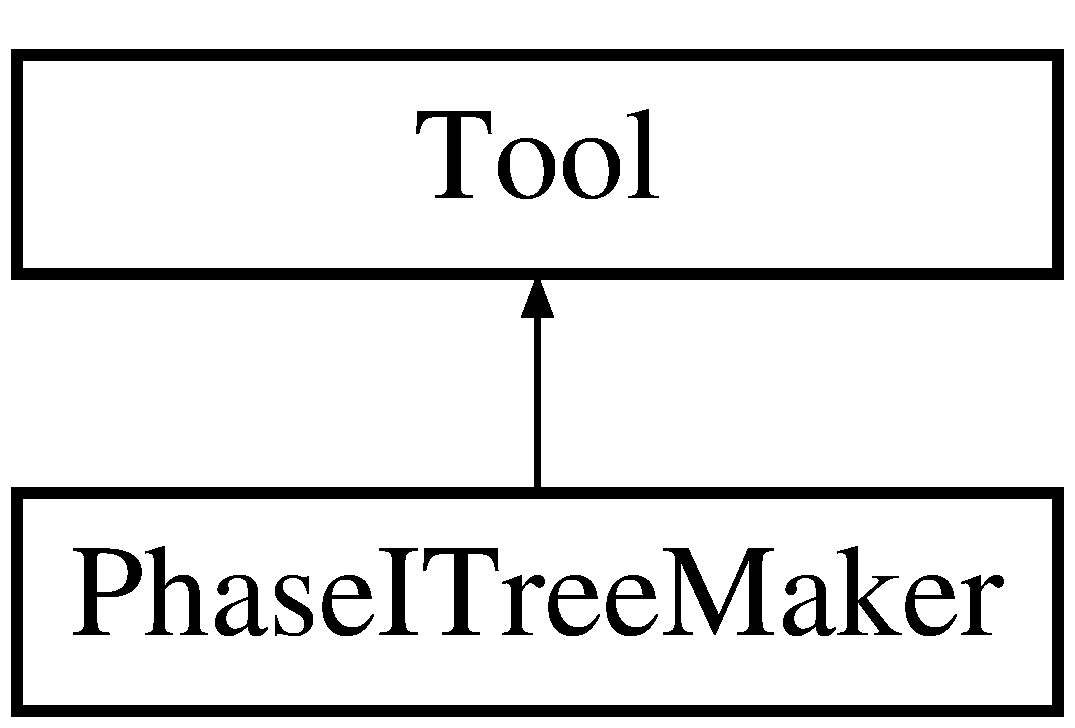
\includegraphics[height=2.000000cm]{classPhaseITreeMaker}
\end{center}
\end{figure}
\subsection*{Public Member Functions}
\begin{DoxyCompactItemize}
\item 
\hypertarget{classPhaseITreeMaker_aa12e20838522941f6a22633bab68f670}{bool {\bfseries Initialise} (const std\-::string configfile, \hyperlink{classDataModel}{Data\-Model} \&data) override}\label{classPhaseITreeMaker_aa12e20838522941f6a22633bab68f670}

\item 
\hypertarget{classPhaseITreeMaker_ad5fc39011665bc920d1f87fdf3315b0c}{bool {\bfseries Execute} () override}\label{classPhaseITreeMaker_ad5fc39011665bc920d1f87fdf3315b0c}

\item 
\hypertarget{classPhaseITreeMaker_a1e910bcd77869d96213501d25a5074ca}{bool {\bfseries Finalise} () override}\label{classPhaseITreeMaker_a1e910bcd77869d96213501d25a5074ca}

\end{DoxyCompactItemize}
\subsection*{Protected Member Functions}
\begin{DoxyCompactItemize}
\item 
\hypertarget{classPhaseITreeMaker_a2353d84241001bec77f48242e0d6545d}{{\footnotesize template$<$typename T , typename A\-Store $>$ }\\bool {\bfseries get\-\_\-object\-\_\-from\-\_\-store} (const std\-::string \&object\-\_\-label, T \&obj, A\-Store \&s)}\label{classPhaseITreeMaker_a2353d84241001bec77f48242e0d6545d}

\item 
\hypertarget{classPhaseITreeMaker_a0cec12d12944459177035800d5206d45}{{\footnotesize template$<$typename T $>$ }\\auto {\bfseries check\-\_\-that\-\_\-not\-\_\-empty} (const std\-::string \&object\-\_\-label, T \&obj) -\/$>$ decltype(std\-::declval$<$ T \& $>$().empty())}\label{classPhaseITreeMaker_a0cec12d12944459177035800d5206d45}

\item 
\hypertarget{classPhaseITreeMaker_af70785f235c6dfc44acd219acc49d2ba}{int {\bfseries get\-\_\-\-N\-C\-V\-\_\-position} (uint32\-\_\-t run\-\_\-number) const }\label{classPhaseITreeMaker_af70785f235c6dfc44acd219acc49d2ba}

\item 
\hypertarget{classPhaseITreeMaker_a4d51e9c4ce60a8f932d3719a24c62494}{bool {\bfseries approve\-\_\-event} (int64\-\_\-t event\-\_\-time, int64\-\_\-t old\-\_\-time, const \hyperlink{classADCPulse}{A\-D\-C\-Pulse} \&first\-\_\-ncv1\-\_\-pulse, const std\-::map$<$ unsigned long, std\-::vector$<$ std\-::vector$<$ \hyperlink{classADCPulse}{A\-D\-C\-Pulse} $>$ $>$ $>$ \&adc\-\_\-hits, int minibuffer\-\_\-index)}\label{classPhaseITreeMaker_a4d51e9c4ce60a8f932d3719a24c62494}

\item 
\hypertarget{classPhaseITreeMaker_aa52d9d62bd39a9883fe2d49b8d92de1b}{double {\bfseries compute\-\_\-tank\-\_\-charge} (size\-\_\-t minibuffer\-\_\-number, const std\-::map$<$ unsigned long, std\-::vector$<$ std\-::vector$<$ \hyperlink{classADCPulse}{A\-D\-C\-Pulse} $>$ $>$ $>$ \&adc\-\_\-hits, uint64\-\_\-t start\-\_\-time, uint64\-\_\-t end\-\_\-time, int \&num\-\_\-unique\-\_\-water\-\_\-pmts)}\label{classPhaseITreeMaker_aa52d9d62bd39a9883fe2d49b8d92de1b}

\end{DoxyCompactItemize}
\subsection*{Protected Attributes}
\begin{DoxyCompactItemize}
\item 
\hypertarget{classPhaseITreeMaker_a75f89b2e33d97896b1d9364a20e542dd}{int \hyperlink{classPhaseITreeMaker_a75f89b2e33d97896b1d9364a20e542dd}{verbosity\-\_\-} = 0}\label{classPhaseITreeMaker_a75f89b2e33d97896b1d9364a20e542dd}

\begin{DoxyCompactList}\small\item\em Integer that determines the level of logging to perform. \end{DoxyCompactList}\item 
\hypertarget{classPhaseITreeMaker_ab43b43c6e78f17bc649edc8b86b0d245}{int \hyperlink{classPhaseITreeMaker_ab43b43c6e78f17bc649edc8b86b0d245}{afterpulsing\-\_\-veto\-\_\-time\-\_\-} = 0}\label{classPhaseITreeMaker_ab43b43c6e78f17bc649edc8b86b0d245}

\begin{DoxyCompactList}\small\item\em The time (in ns) to use when applying the afterpulsing veto. \end{DoxyCompactList}\item 
\hypertarget{classPhaseITreeMaker_a7cfb0cb750c6c6bb5c7d0ece1b837dbb}{int \hyperlink{classPhaseITreeMaker_a7cfb0cb750c6c6bb5c7d0ece1b837dbb}{tank\-\_\-charge\-\_\-window\-\_\-length\-\_\-} = 0}\label{classPhaseITreeMaker_a7cfb0cb750c6c6bb5c7d0ece1b837dbb}

\begin{DoxyCompactList}\small\item\em The time interval over which to compute the tank charge for each N\-C\-V coincidence event. \end{DoxyCompactList}\item 
\hypertarget{classPhaseITreeMaker_a4cf3023fb082c58b2ce75ee63cb60372}{int \hyperlink{classPhaseITreeMaker_a4cf3023fb082c58b2ce75ee63cb60372}{max\-\_\-unique\-\_\-water\-\_\-pmts\-\_\-} = 0}\label{classPhaseITreeMaker_a4cf3023fb082c58b2ce75ee63cb60372}

\begin{DoxyCompactList}\small\item\em The maximum number of unique water P\-M\-Ts to allow for a neutron candidate event. \end{DoxyCompactList}\item 
\hypertarget{classPhaseITreeMaker_a987ef63235bef3d80f1b212ecd6bc5f5}{double \hyperlink{classPhaseITreeMaker_a987ef63235bef3d80f1b212ecd6bc5f5}{max\-\_\-tank\-\_\-charge\-\_\-} = 0.}\label{classPhaseITreeMaker_a987ef63235bef3d80f1b212ecd6bc5f5}

\begin{DoxyCompactList}\small\item\em The maximum tank charge (in n\-C) to allow for a neutron candidate event. \end{DoxyCompactList}\item 
\hypertarget{classPhaseITreeMaker_a5487981246c33caa49c30aa09d6f9d98}{int \hyperlink{classPhaseITreeMaker_a5487981246c33caa49c30aa09d6f9d98}{ncv\-\_\-coincidence\-\_\-tolerance\-\_\-} = 0}\label{classPhaseITreeMaker_a5487981246c33caa49c30aa09d6f9d98}

\begin{DoxyCompactList}\small\item\em The maximum allowed time between N\-C\-V P\-M\-T pulses for them to count as a \char`\"{}coincidence\char`\"{}. \end{DoxyCompactList}\item 
\hypertarget{classPhaseITreeMaker_a67db041338ed358586fb935775b504aa}{std\-::unique\-\_\-ptr$<$ T\-File $>$ \hyperlink{classPhaseITreeMaker_a67db041338ed358586fb935775b504aa}{output\-\_\-tfile\-\_\-} = nullptr}\label{classPhaseITreeMaker_a67db041338ed358586fb935775b504aa}

\begin{DoxyCompactList}\small\item\em R\-O\-O\-T T\-File that will be used to store the output from this tool. \end{DoxyCompactList}\item 
\hypertarget{classPhaseITreeMaker_ac35cd1936f5733ef3c133058727875f4}{T\-Tree $\ast$ \hyperlink{classPhaseITreeMaker_ac35cd1936f5733ef3c133058727875f4}{output\-\_\-tree\-\_\-} = nullptr}\label{classPhaseITreeMaker_ac35cd1936f5733ef3c133058727875f4}

\begin{DoxyCompactList}\small\item\em T\-Tree that will be used to store output. \end{DoxyCompactList}\item 
\hypertarget{classPhaseITreeMaker_ad73a1ddf206e49fbca71fe62d495c69f}{uint32\-\_\-t {\bfseries run\-\_\-number\-\_\-} = 0u}\label{classPhaseITreeMaker_ad73a1ddf206e49fbca71fe62d495c69f}

\item 
\hypertarget{classPhaseITreeMaker_aec7329027d1c43d9ee16a7fcb96bdf17}{uint32\-\_\-t {\bfseries subrun\-\_\-number\-\_\-} = 0u}\label{classPhaseITreeMaker_aec7329027d1c43d9ee16a7fcb96bdf17}

\item 
\hypertarget{classPhaseITreeMaker_a9c8c0cef2793e9059895effb38560991}{uint32\-\_\-t {\bfseries event\-\_\-number\-\_\-} = 0u}\label{classPhaseITreeMaker_a9c8c0cef2793e9059895effb38560991}

\item 
\hypertarget{classPhaseITreeMaker_a841c48bc0851c7aa6ae227964290b9dc}{int {\bfseries ncv\-\_\-position\-\_\-} = 0}\label{classPhaseITreeMaker_a841c48bc0851c7aa6ae227964290b9dc}

\item 
\hypertarget{classPhaseITreeMaker_a0d64443fb0a8c8dcc537f9786e7b295c}{int64\-\_\-t {\bfseries event\-\_\-time\-\_\-ns\-\_\-} = 0}\label{classPhaseITreeMaker_a0d64443fb0a8c8dcc537f9786e7b295c}

\item 
\hypertarget{classPhaseITreeMaker_a0665ba67fb7c02ca95053d4eff0f4976}{uint8\-\_\-t {\bfseries event\-\_\-label\-\_\-} = 0u}\label{classPhaseITreeMaker_a0665ba67fb7c02ca95053d4eff0f4976}

\item 
\hypertarget{classPhaseITreeMaker_a1a94b0cfc66718ea806e5885f08164e2}{bool {\bfseries hefty\-\_\-mode\-\_\-} = false}\label{classPhaseITreeMaker_a1a94b0cfc66718ea806e5885f08164e2}

\item 
\hypertarget{classPhaseITreeMaker_add3f0ad690d2e71cae9b7e299cf91091}{int {\bfseries hefty\-\_\-trigger\-\_\-mask\-\_\-} = 0}\label{classPhaseITreeMaker_add3f0ad690d2e71cae9b7e299cf91091}

\item 
\hypertarget{classPhaseITreeMaker_a9d9ab445ffa95f01f0283864695f44ac}{double {\bfseries amplitude\-\_\-ncv1\-\_\-} = 0.}\label{classPhaseITreeMaker_a9d9ab445ffa95f01f0283864695f44ac}

\item 
\hypertarget{classPhaseITreeMaker_a5b287952c6d649c33e164ee494cf9b52}{double {\bfseries amplitude\-\_\-ncv2\-\_\-} = 0.}\label{classPhaseITreeMaker_a5b287952c6d649c33e164ee494cf9b52}

\item 
\hypertarget{classPhaseITreeMaker_ac1c44250bdff61e88c41d36e7eb99a9c}{double {\bfseries charge\-\_\-ncv1\-\_\-} = 0.}\label{classPhaseITreeMaker_ac1c44250bdff61e88c41d36e7eb99a9c}

\item 
\hypertarget{classPhaseITreeMaker_a7655973b514787a2e4d6fcbb16704361}{double {\bfseries charge\-\_\-ncv2\-\_\-} = 0.}\label{classPhaseITreeMaker_a7655973b514787a2e4d6fcbb16704361}

\item 
\hypertarget{classPhaseITreeMaker_a02aa5dec1ed25dbbc69d6d555daa39e8}{unsigned short {\bfseries raw\-\_\-amplitude\-\_\-ncv1\-\_\-} = 0u}\label{classPhaseITreeMaker_a02aa5dec1ed25dbbc69d6d555daa39e8}

\item 
\hypertarget{classPhaseITreeMaker_a3753af4c4913247283fafc4f966f53ce}{unsigned short {\bfseries raw\-\_\-amplitude\-\_\-ncv2\-\_\-} = 0u}\label{classPhaseITreeMaker_a3753af4c4913247283fafc4f966f53ce}

\item 
\hypertarget{classPhaseITreeMaker_a874c9efb242b5b92e8f8f90c6fd4f23b}{std\-::map$<$ int, \hyperlink{structNCVPositionInfo}{N\-C\-V\-Position\-Info} $>$ {\bfseries ncv\-\_\-position\-\_\-info\-\_\-}}\label{classPhaseITreeMaker_a874c9efb242b5b92e8f8f90c6fd4f23b}

\item 
\hypertarget{classPhaseITreeMaker_aceed975ee31a653ad428312ffed02f97}{T\-Tree $\ast$ {\bfseries output\-\_\-pulse\-\_\-tree\-\_\-} = nullptr}\label{classPhaseITreeMaker_aceed975ee31a653ad428312ffed02f97}

\item 
\hypertarget{classPhaseITreeMaker_a8cbadc4026164224e74e32de446a8e15}{uint32\-\_\-t {\bfseries minibuffer\-\_\-number\-\_\-} = 0u}\label{classPhaseITreeMaker_a8cbadc4026164224e74e32de446a8e15}

\item 
\hypertarget{classPhaseITreeMaker_a83562863bc7bce788d917cd40d31dfe7}{int64\-\_\-t {\bfseries pulse\-\_\-start\-\_\-time\-\_\-ns\-\_\-} = 0}\label{classPhaseITreeMaker_a83562863bc7bce788d917cd40d31dfe7}

\item 
\hypertarget{classPhaseITreeMaker_aa470eceac054608c14062606d64e6e5f}{double {\bfseries pulse\-\_\-amplitude\-\_\-} = 0.}\label{classPhaseITreeMaker_aa470eceac054608c14062606d64e6e5f}

\item 
\hypertarget{classPhaseITreeMaker_a78af37dbe76387f64abb9a82e12842c3}{double {\bfseries pulse\-\_\-charge\-\_\-} = 0.}\label{classPhaseITreeMaker_a78af37dbe76387f64abb9a82e12842c3}

\item 
\hypertarget{classPhaseITreeMaker_a13e66292551f2732d9091ac454178848}{int {\bfseries pulse\-\_\-pmt\-\_\-id\-\_\-} = 0.}\label{classPhaseITreeMaker_a13e66292551f2732d9091ac454178848}

\item 
\hypertarget{classPhaseITreeMaker_a23f2da00ca69a52485044a39f2bc9ee0}{unsigned short {\bfseries pulse\-\_\-raw\-\_\-amplitude\-\_\-} = 0u}\label{classPhaseITreeMaker_a23f2da00ca69a52485044a39f2bc9ee0}

\item 
\hypertarget{classPhaseITreeMaker_a9363a87ceae0d21c75e01db1df6cdd8a}{uint32\-\_\-t {\bfseries spill\-\_\-number\-\_\-} = 0u}\label{classPhaseITreeMaker_a9363a87ceae0d21c75e01db1df6cdd8a}

\item 
\hypertarget{classPhaseITreeMaker_a2abc635b4b7dd1049eb03aea068c727b}{bool {\bfseries in\-\_\-spill\-\_\-} = false}\label{classPhaseITreeMaker_a2abc635b4b7dd1049eb03aea068c727b}

\item 
\hypertarget{classPhaseITreeMaker_a6ed6473e4b74ba6eff55b1121f4bc3b1}{T\-Tree $\ast$ {\bfseries output\-\_\-beam\-\_\-tree\-\_\-} = nullptr}\label{classPhaseITreeMaker_a6ed6473e4b74ba6eff55b1121f4bc3b1}

\item 
\hypertarget{classPhaseITreeMaker_adda325293e3d77024523c447761ff3a3}{bool {\bfseries pot\-\_\-ok\-\_\-} = false}\label{classPhaseITreeMaker_adda325293e3d77024523c447761ff3a3}

\item 
\hypertarget{classPhaseITreeMaker_ad22c1f1d5f83ed60d6cb8d4b38cd1a93}{bool {\bfseries horn\-\_\-current\-\_\-ok\-\_\-} = false}\label{classPhaseITreeMaker_ad22c1f1d5f83ed60d6cb8d4b38cd1a93}

\item 
\hypertarget{classPhaseITreeMaker_ae63bf72fba04f5334a75801b207b76a5}{bool {\bfseries timestamps\-\_\-ok\-\_\-} = false}\label{classPhaseITreeMaker_ae63bf72fba04f5334a75801b207b76a5}

\item 
\hypertarget{classPhaseITreeMaker_aaefb2a68be7c1f78577db8631680304a}{bool {\bfseries toroids\-\_\-agree\-\_\-} = false}\label{classPhaseITreeMaker_aaefb2a68be7c1f78577db8631680304a}

\item 
\hypertarget{classPhaseITreeMaker_a9f95ccc126493c05a7f4ee7a3da86fe2}{\hyperlink{classGeometry}{Geometry} $\ast$ {\bfseries anniegeom} =nullptr}\label{classPhaseITreeMaker_a9f95ccc126493c05a7f4ee7a3da86fe2}

\end{DoxyCompactItemize}


The documentation for this class was generated from the following files\-:\begin{DoxyCompactItemize}
\item 
User\-Tools/\-Phase\-I\-Tree\-Maker/Phase\-I\-Tree\-Maker.\-h\item 
User\-Tools/\-Phase\-I\-Tree\-Maker/Phase\-I\-Tree\-Maker.\-cpp\end{DoxyCompactItemize}

\hypertarget{classPlotLAPPDTimesFromStore}{\section{Plot\-L\-A\-P\-P\-D\-Times\-From\-Store Class Reference}
\label{classPlotLAPPDTimesFromStore}\index{Plot\-L\-A\-P\-P\-D\-Times\-From\-Store@{Plot\-L\-A\-P\-P\-D\-Times\-From\-Store}}
}
Inheritance diagram for Plot\-L\-A\-P\-P\-D\-Times\-From\-Store\-:\begin{figure}[H]
\begin{center}
\leavevmode
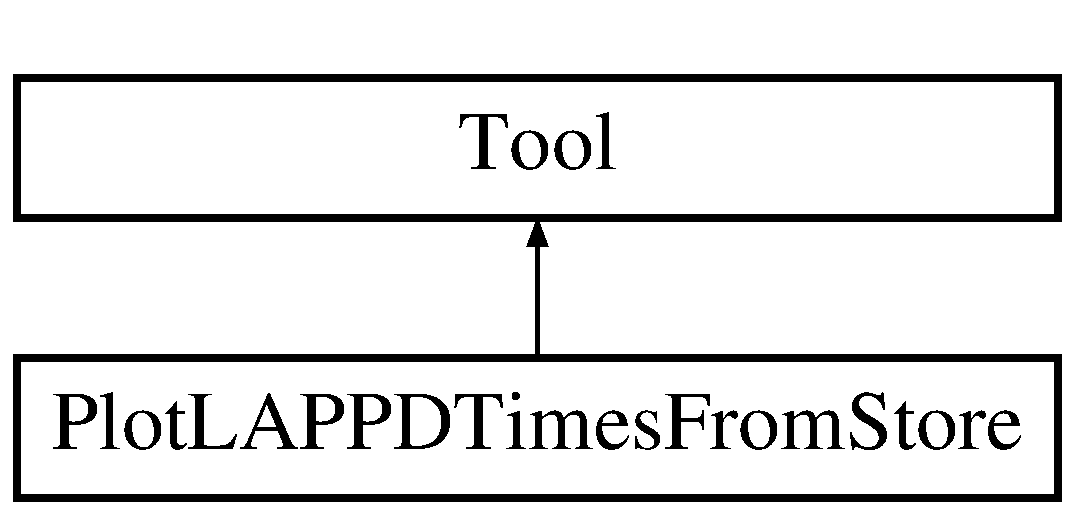
\includegraphics[height=2.000000cm]{classPlotLAPPDTimesFromStore}
\end{center}
\end{figure}
\subsection*{Public Member Functions}
\begin{DoxyCompactItemize}
\item 
\hypertarget{classPlotLAPPDTimesFromStore_a1c22a1c4414885d84bbc496082fc04d3}{bool {\bfseries Initialise} (std\-::string configfile, \hyperlink{classDataModel}{Data\-Model} \&data)}\label{classPlotLAPPDTimesFromStore_a1c22a1c4414885d84bbc496082fc04d3}

\item 
\hypertarget{classPlotLAPPDTimesFromStore_a785fe9ebe3ffe9c8d889eb25323b8ea4}{bool {\bfseries Execute} ()}\label{classPlotLAPPDTimesFromStore_a785fe9ebe3ffe9c8d889eb25323b8ea4}

\item 
\hypertarget{classPlotLAPPDTimesFromStore_a38ddf79485e6f76cf142c90243dcd119}{bool {\bfseries Finalise} ()}\label{classPlotLAPPDTimesFromStore_a38ddf79485e6f76cf142c90243dcd119}

\end{DoxyCompactItemize}


The documentation for this class was generated from the following files\-:\begin{DoxyCompactItemize}
\item 
User\-Tools/\-Plot\-L\-A\-P\-P\-D\-Times\-From\-Store/Plot\-L\-A\-P\-P\-D\-Times\-From\-Store.\-h\item 
User\-Tools/\-Plot\-L\-A\-P\-P\-D\-Times\-From\-Store/Plot\-L\-A\-P\-P\-D\-Times\-From\-Store.\-cpp\end{DoxyCompactItemize}

\hypertarget{classPMTData}{
\section{PMTData Class Reference}
\label{classPMTData}\index{PMTData@{PMTData}}
}
\subsection*{Public Member Functions}
\begin{DoxyCompactItemize}
\item 
\hypertarget{classPMTData_a9fb3e9a250f7d6f53ffd3cd486a6c9ca}{
{\bfseries PMTData} (TTree $\ast$tree=0)}
\label{classPMTData_a9fb3e9a250f7d6f53ffd3cd486a6c9ca}

\item 
\hypertarget{classPMTData_a151bf99e0c8eebea744a35c1388decff}{
virtual Int\_\-t {\bfseries Cut} (Long64\_\-t entry)}
\label{classPMTData_a151bf99e0c8eebea744a35c1388decff}

\item 
\hypertarget{classPMTData_a0773b13bc2ba5ca2cb9f0605aeb747c8}{
virtual Int\_\-t {\bfseries GetEntry} (Long64\_\-t entry)}
\label{classPMTData_a0773b13bc2ba5ca2cb9f0605aeb747c8}

\item 
\hypertarget{classPMTData_a5a3112418d78d73252fd02ebbe17c208}{
virtual Long64\_\-t {\bfseries LoadTree} (Long64\_\-t entry)}
\label{classPMTData_a5a3112418d78d73252fd02ebbe17c208}

\item 
\hypertarget{classPMTData_ac40dd75e44910a6e175c4397ed26caca}{
virtual void {\bfseries Init} (TTree $\ast$tree)}
\label{classPMTData_ac40dd75e44910a6e175c4397ed26caca}

\item 
\hypertarget{classPMTData_a109253ff2e9aee1cb5bbb25627212c34}{
virtual void {\bfseries Loop} ()}
\label{classPMTData_a109253ff2e9aee1cb5bbb25627212c34}

\item 
\hypertarget{classPMTData_a24e98a85f082df3ad82dc69e9004d97d}{
virtual Bool\_\-t {\bfseries Notify} ()}
\label{classPMTData_a24e98a85f082df3ad82dc69e9004d97d}

\item 
\hypertarget{classPMTData_a486dd48b9431a34fa8126566e7c5af07}{
virtual void {\bfseries Show} (Long64\_\-t entry=-\/1)}
\label{classPMTData_a486dd48b9431a34fa8126566e7c5af07}

\end{DoxyCompactItemize}
\subsection*{Public Attributes}
\begin{DoxyCompactItemize}
\item 
\hypertarget{classPMTData_ab6f5a263a14b5dd5f6e35ca1df4ca7f2}{
TTree $\ast$ {\bfseries fChain}}
\label{classPMTData_ab6f5a263a14b5dd5f6e35ca1df4ca7f2}

\item 
\hypertarget{classPMTData_a7745fca9e7cc842de4b0b57407b77f88}{
Int\_\-t \hyperlink{classPMTData_a7745fca9e7cc842de4b0b57407b77f88}{fCurrent}}
\label{classPMTData_a7745fca9e7cc842de4b0b57407b77f88}

\begin{DoxyCompactList}\small\item\em pointer to the analyzed TTree or TChain \item\end{DoxyCompactList}\item 
\hypertarget{classPMTData_aca229b56ff1777b30c95f5325cc55292}{
ULong64\_\-t \hyperlink{classPMTData_aca229b56ff1777b30c95f5325cc55292}{LastSync}}
\label{classPMTData_aca229b56ff1777b30c95f5325cc55292}

\begin{DoxyCompactList}\small\item\em current Tree number in a TChain \item\end{DoxyCompactList}\item 
\hypertarget{classPMTData_a5c6be7f17efe083ea5a5df3921ddef80}{
Int\_\-t {\bfseries SequenceID}}
\label{classPMTData_a5c6be7f17efe083ea5a5df3921ddef80}

\item 
\hypertarget{classPMTData_a4c0df523145834151778799e8f3fa223}{
Int\_\-t {\bfseries StartTimeSec}}
\label{classPMTData_a4c0df523145834151778799e8f3fa223}

\item 
\hypertarget{classPMTData_aa2983c2163daa5b6460706e00d5f9097}{
Int\_\-t {\bfseries StartTimeNSec}}
\label{classPMTData_aa2983c2163daa5b6460706e00d5f9097}

\item 
\hypertarget{classPMTData_a6aff50e9830483d158ec19db4e739144}{
ULong64\_\-t {\bfseries StartCount}}
\label{classPMTData_a6aff50e9830483d158ec19db4e739144}

\item 
\hypertarget{classPMTData_a7731940755b54f0aaa070918452f9808}{
Int\_\-t {\bfseries TriggerNumber}}
\label{classPMTData_a7731940755b54f0aaa070918452f9808}

\item 
\hypertarget{classPMTData_a3e8a744ca7404c04599e057b70c0db1a}{
ULong64\_\-t {\bfseries TriggerCounts} \mbox{[}1000\mbox{]}}
\label{classPMTData_a3e8a744ca7404c04599e057b70c0db1a}

\item 
\hypertarget{classPMTData_aa3a2c054e9edff3b65451442ef8b2626}{
Int\_\-t {\bfseries CardID}}
\label{classPMTData_aa3a2c054e9edff3b65451442ef8b2626}

\item 
\hypertarget{classPMTData_ac39a7f82be7ed720d6ce21ff613a656c}{
Int\_\-t {\bfseries Channels}}
\label{classPMTData_ac39a7f82be7ed720d6ce21ff613a656c}

\item 
\hypertarget{classPMTData_ad91fc40f8e3ce0aabbe1648fa560f62d}{
UInt\_\-t {\bfseries Rates} \mbox{[}4\mbox{]}}
\label{classPMTData_ad91fc40f8e3ce0aabbe1648fa560f62d}

\item 
\hypertarget{classPMTData_a39ad6ca7b1c7cd326fe596a89fb298b5}{
Int\_\-t {\bfseries BufferSize}}
\label{classPMTData_a39ad6ca7b1c7cd326fe596a89fb298b5}

\item 
\hypertarget{classPMTData_a8f813e3178ccac6319e97cbb7cfee21b}{
Int\_\-t {\bfseries Eventsize}}
\label{classPMTData_a8f813e3178ccac6319e97cbb7cfee21b}

\item 
\hypertarget{classPMTData_a13cb45d719516d2bcbde3cd4eef55e04}{
Int\_\-t {\bfseries FullBufferSize}}
\label{classPMTData_a13cb45d719516d2bcbde3cd4eef55e04}

\item 
\hypertarget{classPMTData_a43a7b1b166157c159aa1efe8420134b3}{
UShort\_\-t {\bfseries Data} \mbox{[}160000\mbox{]}}
\label{classPMTData_a43a7b1b166157c159aa1efe8420134b3}

\item 
\hypertarget{classPMTData_abc6551b1d8772098c4d5b395d06ff1e6}{
TBranch $\ast$ {\bfseries b\_\-LastSync}}
\label{classPMTData_abc6551b1d8772098c4d5b395d06ff1e6}

\item 
\hypertarget{classPMTData_ab9df240954636c9ddb2dc01f028fd1e2}{
TBranch $\ast$ {\bfseries b\_\-SequenceID}}
\label{classPMTData_ab9df240954636c9ddb2dc01f028fd1e2}

\item 
\hypertarget{classPMTData_a928c9e3c2f801f970537a5c5ff5eec3e}{
TBranch $\ast$ {\bfseries b\_\-StartTimeSec}}
\label{classPMTData_a928c9e3c2f801f970537a5c5ff5eec3e}

\item 
\hypertarget{classPMTData_adf7cd7729bb5bba9ad630deb52f59946}{
TBranch $\ast$ {\bfseries b\_\-StartTimeNSec}}
\label{classPMTData_adf7cd7729bb5bba9ad630deb52f59946}

\item 
\hypertarget{classPMTData_a76e691f68bd678cfcee9abd08ac96ed6}{
TBranch $\ast$ {\bfseries b\_\-StartCount}}
\label{classPMTData_a76e691f68bd678cfcee9abd08ac96ed6}

\item 
\hypertarget{classPMTData_a086214097320d5797cc153f1b27f0bef}{
TBranch $\ast$ {\bfseries b\_\-TriggerNumber}}
\label{classPMTData_a086214097320d5797cc153f1b27f0bef}

\item 
\hypertarget{classPMTData_a9265633fa545a406faeda273716b3e11}{
TBranch $\ast$ {\bfseries b\_\-TriggerCounts}}
\label{classPMTData_a9265633fa545a406faeda273716b3e11}

\item 
\hypertarget{classPMTData_a6f2ac15158ae8a458f56cce652ea9f6d}{
TBranch $\ast$ {\bfseries b\_\-CardID}}
\label{classPMTData_a6f2ac15158ae8a458f56cce652ea9f6d}

\item 
\hypertarget{classPMTData_ac08cb29ec61c1d945fbf6893c2f80b90}{
TBranch $\ast$ {\bfseries b\_\-Channels}}
\label{classPMTData_ac08cb29ec61c1d945fbf6893c2f80b90}

\item 
\hypertarget{classPMTData_a29343471536481bcfa94d746958018d2}{
TBranch $\ast$ {\bfseries b\_\-Rates}}
\label{classPMTData_a29343471536481bcfa94d746958018d2}

\item 
\hypertarget{classPMTData_a4df357ba10b131aa5a2886ccf08899fa}{
TBranch $\ast$ {\bfseries b\_\-BufferSize}}
\label{classPMTData_a4df357ba10b131aa5a2886ccf08899fa}

\item 
\hypertarget{classPMTData_a66261088f4371dc96d62f508178e6a91}{
TBranch $\ast$ {\bfseries b\_\-Eventsize}}
\label{classPMTData_a66261088f4371dc96d62f508178e6a91}

\item 
\hypertarget{classPMTData_a26d8366646579d0a26a951c9bde9a6b0}{
TBranch $\ast$ {\bfseries b\_\-FullBufferSize}}
\label{classPMTData_a26d8366646579d0a26a951c9bde9a6b0}

\item 
\hypertarget{classPMTData_a19565c90684786dc6221282ba7e1305c}{
TBranch $\ast$ {\bfseries b\_\-Data}}
\label{classPMTData_a19565c90684786dc6221282ba7e1305c}

\end{DoxyCompactItemize}


The documentation for this class was generated from the following files:\begin{DoxyCompactItemize}
\item 
UserTools/LoadCCData/PMTData.h\item 
UserTools/LoadCCData/PMTData.cpp\end{DoxyCompactItemize}

\hypertarget{classPosition}{\section{Position Class Reference}
\label{classPosition}\index{Position@{Position}}
}
Inheritance diagram for Position\-:\begin{figure}[H]
\begin{center}
\leavevmode
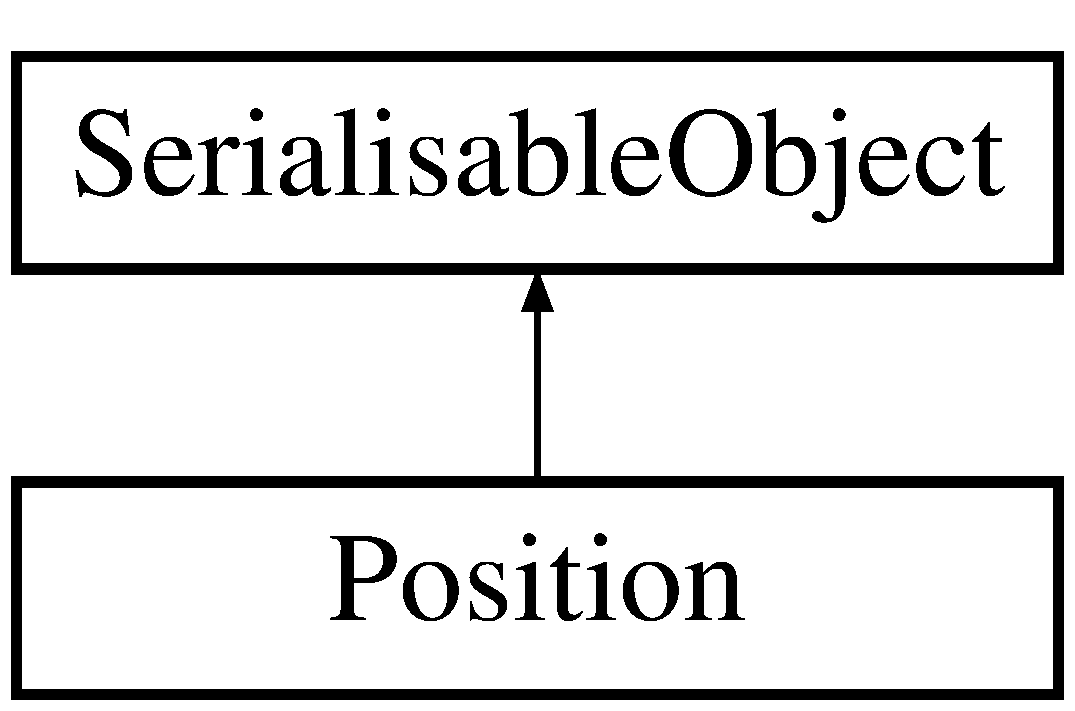
\includegraphics[height=2.000000cm]{classPosition}
\end{center}
\end{figure}
\subsection*{Public Member Functions}
\begin{DoxyCompactItemize}
\item 
\hypertarget{classPosition_a324c80892d3dcba7c99319102f9ca9ed}{{\bfseries Position} (double xin, double yin, double zin)}\label{classPosition_a324c80892d3dcba7c99319102f9ca9ed}

\item 
\hypertarget{classPosition_a7d829a2e612447d00d7965714045bb9a}{double {\bfseries X} () const }\label{classPosition_a7d829a2e612447d00d7965714045bb9a}

\item 
\hypertarget{classPosition_a2d318ced6e936e9c18225a290a32fdcb}{double {\bfseries Y} () const }\label{classPosition_a2d318ced6e936e9c18225a290a32fdcb}

\item 
\hypertarget{classPosition_aa57d77c97e6a3ef617ff5227053de6af}{double {\bfseries Z} () const }\label{classPosition_aa57d77c97e6a3ef617ff5227053de6af}

\item 
\hypertarget{classPosition_a3ea3a7594f1c164ceb06053f0e3fac02}{void {\bfseries Set\-X} (double xx)}\label{classPosition_a3ea3a7594f1c164ceb06053f0e3fac02}

\item 
\hypertarget{classPosition_a6a288f1fe2c5f642bba613828f2f38e2}{void {\bfseries Set\-Y} (double yy)}\label{classPosition_a6a288f1fe2c5f642bba613828f2f38e2}

\item 
\hypertarget{classPosition_a70362eb60d97b0229f234f3e72fbf625}{void {\bfseries Set\-Z} (double zz)}\label{classPosition_a70362eb60d97b0229f234f3e72fbf625}

\item 
\hypertarget{classPosition_aeb4bd6d16d803853b477d9fb08078619}{double {\bfseries Get\-Phi} ()}\label{classPosition_aeb4bd6d16d803853b477d9fb08078619}

\item 
\hypertarget{classPosition_a2abfd5065053d48f6d7808b1b024a07e}{double {\bfseries Get\-Theta} ()}\label{classPosition_a2abfd5065053d48f6d7808b1b024a07e}

\item 
\hypertarget{classPosition_a9d6bafb2c4b8e4a69aed1ec717f0a898}{double {\bfseries Get\-R} ()}\label{classPosition_a9d6bafb2c4b8e4a69aed1ec717f0a898}

\item 
\hypertarget{classPosition_a917945e24d7307e45658e0d45596eab9}{void {\bfseries Unit\-To\-Centimeter} ()}\label{classPosition_a917945e24d7307e45658e0d45596eab9}

\item 
\hypertarget{classPosition_af02152e9534534c2b21414ee26435da9}{void {\bfseries Unit\-To\-Meter} ()}\label{classPosition_af02152e9534534c2b21414ee26435da9}

\item 
\hypertarget{classPosition_aa795d01e1825aec571603081412aedab}{\hyperlink{classPosition}{Position} {\bfseries Unit} ()}\label{classPosition_aa795d01e1825aec571603081412aedab}

\item 
\hypertarget{classPosition_acc7380659f848eac5268337a893fd264}{double {\bfseries M} () const }\label{classPosition_acc7380659f848eac5268337a893fd264}

\item 
\hypertarget{classPosition_abc9a94774679003228dbb648f481a004}{double {\bfseries M2} () const }\label{classPosition_abc9a94774679003228dbb648f481a004}

\item 
\hypertarget{classPosition_a9e1f77cfa7961674ce9b3fed6488786d}{bool {\bfseries Print} (bool withendline) const }\label{classPosition_a9e1f77cfa7961674ce9b3fed6488786d}

\item 
\hypertarget{classPosition_a65491aa32b851bf35260a5d82a9735da}{bool {\bfseries Print} ()}\label{classPosition_a65491aa32b851bf35260a5d82a9735da}

\item 
\hypertarget{classPosition_aa89951f4ed590fe130ddad8e8809c49f}{bool {\bfseries operator==} (const \hyperlink{classPosition}{Position} \&a) const }\label{classPosition_aa89951f4ed590fe130ddad8e8809c49f}

\item 
\hypertarget{classPosition_a2c041236d9451b265b13d275fabde180}{bool {\bfseries operator!=} (const \hyperlink{classPosition}{Position} \&a) const }\label{classPosition_a2c041236d9451b265b13d275fabde180}

\item 
\hypertarget{classPosition_a0cf399ae7029706e94199ad882383e02}{{\footnotesize template$<$typename T $>$ }\\\hyperlink{classPosition}{Position} {\bfseries operator$\ast$=} (T a)}\label{classPosition_a0cf399ae7029706e94199ad882383e02}

\item 
\hypertarget{classPosition_a195ed1edccd36180b1b7c36025630d71}{\hyperlink{classPosition}{Position} {\bfseries operator-\/} () const }\label{classPosition_a195ed1edccd36180b1b7c36025630d71}

\item 
\hypertarget{classPosition_a2d414d082486e40bef80c1ae3f3d05e7}{\hyperlink{classPosition}{Position} \& {\bfseries operator-\/=} (const \hyperlink{classPosition}{Position} \&b)}\label{classPosition_a2d414d082486e40bef80c1ae3f3d05e7}

\item 
\hypertarget{classPosition_ad2bd309438b9410f3e02b01f6d3db5bc}{\hyperlink{classPosition}{Position} \& {\bfseries operator+=} (const \hyperlink{classPosition}{Position} \&b)}\label{classPosition_ad2bd309438b9410f3e02b01f6d3db5bc}

\item 
\hypertarget{classPosition_a7b9b6ac6629131398f2928360f20eb08}{double {\bfseries Dot} (const \hyperlink{classPosition}{Position} \&p) const }\label{classPosition_a7b9b6ac6629131398f2928360f20eb08}

\item 
\hypertarget{classPosition_ad00bec35610db4f6955a473e24fb7cbb}{\hyperlink{classPosition}{Position} {\bfseries Cross} (const \hyperlink{classPosition}{Position} \&p) const }\label{classPosition_ad00bec35610db4f6955a473e24fb7cbb}

\item 
\hypertarget{classPosition_a03df8eb4c0cc7c341a5424f622faa655}{double {\bfseries Mag2} () const }\label{classPosition_a03df8eb4c0cc7c341a5424f622faa655}

\item 
\hypertarget{classPosition_a5166f113ddb9e5f116ac4e3f6bd638c5}{double {\bfseries Mag} () const }\label{classPosition_a5166f113ddb9e5f116ac4e3f6bd638c5}

\item 
\hypertarget{classPosition_a3140c87b9934338c610c39b8fd300384}{double {\bfseries Angle} (const \hyperlink{classPosition}{Position} \&q) const }\label{classPosition_a3140c87b9934338c610c39b8fd300384}

\item 
\hypertarget{classPosition_afea0aaa9328d8831f89fc491a3fe1cdc}{\hyperlink{classPosition}{Position} {\bfseries Orthogonal} () const }\label{classPosition_afea0aaa9328d8831f89fc491a3fe1cdc}

\item 
\hypertarget{classPosition_ac343878fec78550e928730f27b11cd39}{double {\bfseries Perp2} () const }\label{classPosition_ac343878fec78550e928730f27b11cd39}

\item 
\hypertarget{classPosition_aea7d37f6f8c91f121bd3b814ed0a057f}{double {\bfseries Perp2} (const \hyperlink{classPosition}{Position} \&p) const }\label{classPosition_aea7d37f6f8c91f121bd3b814ed0a057f}

\end{DoxyCompactItemize}
\subsection*{Friends}
\begin{DoxyCompactItemize}
\item 
\hypertarget{classPosition_ac98d07dd8f7b70e16ccb9a01abf56b9c}{class {\bfseries boost\-::serialization\-::access}}\label{classPosition_ac98d07dd8f7b70e16ccb9a01abf56b9c}

\end{DoxyCompactItemize}


The documentation for this class was generated from the following file\-:\begin{DoxyCompactItemize}
\item 
Data\-Model/Position.\-h\end{DoxyCompactItemize}

\hypertarget{classPrintANNIEEvent}{\section{Print\-A\-N\-N\-I\-E\-Event Class Reference}
\label{classPrintANNIEEvent}\index{Print\-A\-N\-N\-I\-E\-Event@{Print\-A\-N\-N\-I\-E\-Event}}
}
Inheritance diagram for Print\-A\-N\-N\-I\-E\-Event\-:\begin{figure}[H]
\begin{center}
\leavevmode
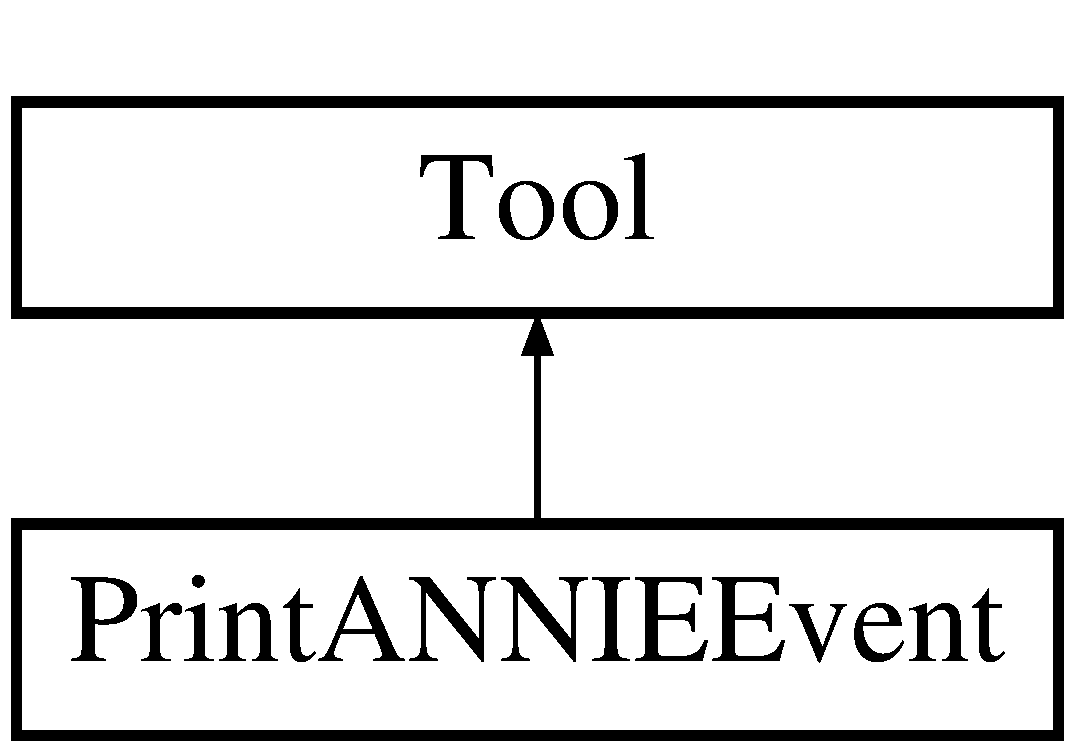
\includegraphics[height=2.000000cm]{classPrintANNIEEvent}
\end{center}
\end{figure}
\subsection*{Public Member Functions}
\begin{DoxyCompactItemize}
\item 
\hypertarget{classPrintANNIEEvent_a837c3af8455ac4ad69218de09e1a9904}{bool {\bfseries Initialise} (std\-::string configfile, \hyperlink{classDataModel}{Data\-Model} \&data)}\label{classPrintANNIEEvent_a837c3af8455ac4ad69218de09e1a9904}

\item 
\hypertarget{classPrintANNIEEvent_aebc14f16147292bfe4c9dcd0b433bee2}{bool {\bfseries Execute} ()}\label{classPrintANNIEEvent_aebc14f16147292bfe4c9dcd0b433bee2}

\item 
\hypertarget{classPrintANNIEEvent_a164df9cb5bd54feadb715dd0a73eb9d3}{bool {\bfseries Finalise} ()}\label{classPrintANNIEEvent_a164df9cb5bd54feadb715dd0a73eb9d3}

\end{DoxyCompactItemize}


The documentation for this class was generated from the following files\-:\begin{DoxyCompactItemize}
\item 
User\-Tools/\-Print\-A\-N\-N\-I\-E\-Event/Print\-A\-N\-N\-I\-E\-Event.\-h\item 
User\-Tools/\-Print\-A\-N\-N\-I\-E\-Event/Print\-A\-N\-N\-I\-E\-Event.\-cpp\end{DoxyCompactItemize}

\hypertarget{classPulseSimulation}{
\section{PulseSimulation Class Reference}
\label{classPulseSimulation}\index{PulseSimulation@{PulseSimulation}}
}
\subsection*{Public Member Functions}
\begin{DoxyCompactItemize}
\item 
\hypertarget{classPulseSimulation_a58b5d01a88aa646f8f89ec60372fdfec}{
bool {\bfseries Initialise} (std::string configfile, \hyperlink{classDataModel}{DataModel} \&data)}
\label{classPulseSimulation_a58b5d01a88aa646f8f89ec60372fdfec}

\item 
\hypertarget{classPulseSimulation_ae65d207c87254a420c4b25172354bef7}{
bool {\bfseries Execute} ()}
\label{classPulseSimulation_ae65d207c87254a420c4b25172354bef7}

\item 
\hypertarget{classPulseSimulation_a8a798184a88f99597de1266fe34fed10}{
bool {\bfseries Finalise} ()}
\label{classPulseSimulation_a8a798184a88f99597de1266fe34fed10}

\end{DoxyCompactItemize}


The documentation for this class was generated from the following files:\begin{DoxyCompactItemize}
\item 
UserTools/PulseSimulation/PulseSimulation.h\item 
UserTools/PulseSimulation/CreateFakeRawFile.cpp\item 
UserTools/PulseSimulation/FillEmulatedCCData.cpp\item 
UserTools/PulseSimulation/FillEmulatedTriggerdata.cpp\item 
UserTools/PulseSimulation/GetTemplateRunInfo.cpp\item 
UserTools/PulseSimulation/PulseSimulation.cpp\end{DoxyCompactItemize}

\hypertarget{classPythonScript}{
\section{PythonScript Class Reference}
\label{classPythonScript}\index{PythonScript@{PythonScript}}
}
\subsection*{Public Member Functions}
\begin{DoxyCompactItemize}
\item 
bool \hyperlink{classPythonScript_aad6cc6780450e409d2a242c6f4eb3d9a}{Initialise} (std::string configfile, \hyperlink{classDataModel}{DataModel} \&data)
\item 
\hypertarget{classPythonScript_a49e8baf3660437e7257327c2e521fbae}{
bool {\bfseries Execute} ()}
\label{classPythonScript_a49e8baf3660437e7257327c2e521fbae}

\item 
\hypertarget{classPythonScript_ada47375997eb9d29a34f5e88aab016f7}{
bool {\bfseries Finalise} ()}
\label{classPythonScript_ada47375997eb9d29a34f5e88aab016f7}

\end{DoxyCompactItemize}


\subsection{Member Function Documentation}
\hypertarget{classPythonScript_aad6cc6780450e409d2a242c6f4eb3d9a}{
\index{PythonScript@{PythonScript}!Initialise@{Initialise}}
\index{Initialise@{Initialise}!PythonScript@{PythonScript}}
\subsubsection[{Initialise}]{\setlength{\rightskip}{0pt plus 5cm}bool PythonScript::Initialise (std::string {\em configfile}, \/  {\bf DataModel} \& {\em data})}}
\label{classPythonScript_aad6cc6780450e409d2a242c6f4eb3d9a}


Starting python thread for this tool 

The documentation for this class was generated from the following files:\begin{DoxyCompactItemize}
\item 
UserTools/PythonScript/PythonScript.h\item 
UserTools/PythonScript/PythonScript.cpp\end{DoxyCompactItemize}

\hypertarget{structquaternion}{\section{quaternion Struct Reference}
\label{structquaternion}\index{quaternion@{quaternion}}
}
\subsection*{Public Attributes}
\begin{DoxyCompactItemize}
\item 
\hypertarget{structquaternion_a70001dd0b39421c936b6d20e15471b3d}{double {\bfseries q0}}\label{structquaternion_a70001dd0b39421c936b6d20e15471b3d}

\item 
\hypertarget{structquaternion_abbdc170dc2ac800c39fab9aa9f99d3ce}{double {\bfseries q1}}\label{structquaternion_abbdc170dc2ac800c39fab9aa9f99d3ce}

\item 
\hypertarget{structquaternion_a7af6afcba00a35e14ab605b11223b83c}{double {\bfseries q2}}\label{structquaternion_a7af6afcba00a35e14ab605b11223b83c}

\item 
\hypertarget{structquaternion_ad6a829c1635921b61464c75903b71dc8}{double {\bfseries q3}}\label{structquaternion_ad6a829c1635921b61464c75903b71dc8}

\end{DoxyCompactItemize}


The documentation for this struct was generated from the following file\-:\begin{DoxyCompactItemize}
\item 
User\-Tools/\-Event\-Display/Event\-Display.\-cpp\end{DoxyCompactItemize}

\hypertarget{classannie_1_1RawAnalyzer}{
\section{annie::RawAnalyzer Class Reference}
\label{classannie_1_1RawAnalyzer}\index{annie::RawAnalyzer@{annie::RawAnalyzer}}
}


Singleton analyzer class for reconstructing ANNIE events from the raw data.  


{\ttfamily \#include $<$RawAnalyzer.h$>$}\subsection*{Public Member Functions}
\begin{DoxyCompactItemize}
\item 
\hypertarget{classannie_1_1RawAnalyzer_aad70827f2e0cf755a655c0013a99a301}{
\hyperlink{classannie_1_1RawAnalyzer_aad70827f2e0cf755a655c0013a99a301}{RawAnalyzer} (const \hyperlink{classannie_1_1RawAnalyzer}{RawAnalyzer} \&)}
\label{classannie_1_1RawAnalyzer_aad70827f2e0cf755a655c0013a99a301}

\begin{DoxyCompactList}\small\item\em Deleted copy constructor. \item\end{DoxyCompactList}\item 
\hypertarget{classannie_1_1RawAnalyzer_a8105363307f1f568f90b3dadd3f1dbf0}{
\hyperlink{classannie_1_1RawAnalyzer_a8105363307f1f568f90b3dadd3f1dbf0}{RawAnalyzer} (\hyperlink{classannie_1_1RawAnalyzer}{RawAnalyzer} \&\&)}
\label{classannie_1_1RawAnalyzer_a8105363307f1f568f90b3dadd3f1dbf0}

\begin{DoxyCompactList}\small\item\em Deleted move constructor. \item\end{DoxyCompactList}\item 
\hypertarget{classannie_1_1RawAnalyzer_a9ee50418cb10e51da8bdbf29fd2241e0}{
\hyperlink{classannie_1_1RawAnalyzer}{RawAnalyzer} \& \hyperlink{classannie_1_1RawAnalyzer_a9ee50418cb10e51da8bdbf29fd2241e0}{operator=} (const \hyperlink{classannie_1_1RawAnalyzer}{RawAnalyzer} \&)}
\label{classannie_1_1RawAnalyzer_a9ee50418cb10e51da8bdbf29fd2241e0}

\begin{DoxyCompactList}\small\item\em Deleted copy assignment operator. \item\end{DoxyCompactList}\item 
\hypertarget{classannie_1_1RawAnalyzer_a50088150eebb6b5f1043544a7f07924a}{
\hyperlink{classannie_1_1RawAnalyzer}{RawAnalyzer} \& \hyperlink{classannie_1_1RawAnalyzer_a50088150eebb6b5f1043544a7f07924a}{operator=} (\hyperlink{classannie_1_1RawAnalyzer}{RawAnalyzer} \&\&)}
\label{classannie_1_1RawAnalyzer_a50088150eebb6b5f1043544a7f07924a}

\begin{DoxyCompactList}\small\item\em Deleted move assignment operator. \item\end{DoxyCompactList}\item 
\hypertarget{classannie_1_1RawAnalyzer_ae71304d77ec7309755408850c6df2848}{
std::vector$<$ \hyperlink{classannie_1_1RecoPulse}{RecoPulse} $>$ {\bfseries find\_\-pulses} (const \hyperlink{classannie_1_1RawChannel}{annie::RawChannel} \&channel, unsigned short adc\_\-threshold) const }
\label{classannie_1_1RawAnalyzer_ae71304d77ec7309755408850c6df2848}

\item 
\hypertarget{classannie_1_1RawAnalyzer_a7a07548a1aa7a73e7fc06553ea55f885}{
std::vector$<$ \hyperlink{classannie_1_1RecoPulse}{annie::RecoPulse} $>$ {\bfseries find\_\-pulses} (const std::vector$<$ unsigned short $>$ \&minibuffer\_\-waveform, double baseline, double sigma\_\-baseline, unsigned short adc\_\-threshold) const }
\label{classannie_1_1RawAnalyzer_a7a07548a1aa7a73e7fc06553ea55f885}

\item 
\hypertarget{classannie_1_1RawAnalyzer_ad0381d0696ff97227c3c307dd42e3f3f}{
std::unique\_\-ptr$<$ \hyperlink{classannie_1_1RecoReadout}{annie::RecoReadout} $>$ {\bfseries find\_\-pulses} (const \hyperlink{classannie_1_1RawReadout}{annie::RawReadout} \&raw\_\-readout) const }
\label{classannie_1_1RawAnalyzer_ad0381d0696ff97227c3c307dd42e3f3f}

\end{DoxyCompactItemize}
\subsection*{Static Public Member Functions}
\begin{DoxyCompactItemize}
\item 
\hypertarget{classannie_1_1RawAnalyzer_a830d493693fd7c5e567b4fd592745d81}{
static const \hyperlink{classannie_1_1RawAnalyzer}{RawAnalyzer} \& \hyperlink{classannie_1_1RawAnalyzer_a830d493693fd7c5e567b4fd592745d81}{Instance} ()}
\label{classannie_1_1RawAnalyzer_a830d493693fd7c5e567b4fd592745d81}

\begin{DoxyCompactList}\small\item\em Get a const reference to the singleton instance of the \hyperlink{classannie_1_1RawAnalyzer}{RawAnalyzer}. \item\end{DoxyCompactList}\end{DoxyCompactItemize}
\subsection*{Protected Member Functions}
\begin{DoxyCompactItemize}
\item 
\hypertarget{classannie_1_1RawAnalyzer_abf612bfdacdea2908e138016e2eb0080}{
\hyperlink{classannie_1_1RawAnalyzer_abf612bfdacdea2908e138016e2eb0080}{RawAnalyzer} ()}
\label{classannie_1_1RawAnalyzer_abf612bfdacdea2908e138016e2eb0080}

\begin{DoxyCompactList}\small\item\em Create the singleton \hyperlink{classannie_1_1RawAnalyzer}{RawAnalyzer} object. \item\end{DoxyCompactList}\item 
void \hyperlink{classannie_1_1RawAnalyzer_a33d2f06b95aa38e099d735809a80c085}{ze3ra\_\-baseline} (const \hyperlink{classannie_1_1RawChannel}{annie::RawChannel} \&channel, double \&baseline, double \&sigma\_\-baseline, size\_\-t num\_\-baseline\_\-samples=DEFAULT\_\-NUM\_\-BASELINE\_\-SAMPLES) const 
\begin{DoxyCompactList}\small\item\em Compute the baseline for a particular \hyperlink{classannie_1_1RawChannel}{RawChannel} object using a technique taken from the ZE3RA code. \item\end{DoxyCompactList}\end{DoxyCompactItemize}
\subsection*{Static Protected Attributes}
\begin{DoxyCompactItemize}
\item 
\hypertarget{classannie_1_1RawAnalyzer_af2922e3755357bc385d3bb0698927da8}{
static constexpr size\_\-t {\bfseries DEFAULT\_\-NUM\_\-BASELINE\_\-SAMPLES} = 25}
\label{classannie_1_1RawAnalyzer_af2922e3755357bc385d3bb0698927da8}

\end{DoxyCompactItemize}


\subsection{Detailed Description}
Singleton analyzer class for reconstructing ANNIE events from the raw data. 

\subsection{Member Function Documentation}
\hypertarget{classannie_1_1RawAnalyzer_a33d2f06b95aa38e099d735809a80c085}{
\index{annie::RawAnalyzer@{annie::RawAnalyzer}!ze3ra\_\-baseline@{ze3ra\_\-baseline}}
\index{ze3ra\_\-baseline@{ze3ra\_\-baseline}!annie::RawAnalyzer@{annie::RawAnalyzer}}
\subsubsection[{ze3ra\_\-baseline}]{\setlength{\rightskip}{0pt plus 5cm}void annie::RawAnalyzer::ze3ra\_\-baseline (const {\bf annie::RawChannel} \& {\em channel}, \/  double \& {\em baseline}, \/  double \& {\em sigma\_\-baseline}, \/  size\_\-t {\em num\_\-baseline\_\-samples} = {\ttfamily DEFAULT\_\-NUM\_\-BASELINE\_\-SAMPLES}) const\hspace{0.3cm}{\ttfamily  \mbox{[}protected\mbox{]}}}}
\label{classannie_1_1RawAnalyzer_a33d2f06b95aa38e099d735809a80c085}


Compute the baseline for a particular \hyperlink{classannie_1_1RawChannel}{RawChannel} object using a technique taken from the ZE3RA code. See section 2.2 of \href{https://arxiv.org/pdf/1106.0808.pdf}{\tt https://arxiv.org/pdf/1106.0808.pdf} for a full description of the algorithm. 

The documentation for this class was generated from the following files:\begin{DoxyCompactItemize}
\item 
UserTools/recoANNIE/RawAnalyzer.h\item 
UserTools/recoANNIE/RawAnalyzer.cc\end{DoxyCompactItemize}

\hypertarget{classannie_1_1RawCard}{
\section{annie::RawCard Class Reference}
\label{classannie_1_1RawCard}\index{annie::RawCard@{annie::RawCard}}
}
\subsection*{Public Member Functions}
\begin{DoxyCompactItemize}
\item 
\hypertarget{classannie_1_1RawCard_ab60fad3bbc6ac3ef66759f4436a57413}{
{\bfseries RawCard} (int CardID, unsigned long long LastSync, int StartTimeSec, int StartTimeNSec, unsigned long long StartCount, int Channels, int BufferSize, int MiniBufferSize, const std::vector$<$ unsigned short $>$ \&Data, const std::vector$<$ unsigned long long $>$ \&TriggerCounts, const std::vector$<$ unsigned int $>$ \&Rates)}
\label{classannie_1_1RawCard_ab60fad3bbc6ac3ef66759f4436a57413}

\item 
\hypertarget{classannie_1_1RawCard_ae80499190a7ce2c3b2b178e9cb2c1aef}{
unsigned int {\bfseries card\_\-id} () const }
\label{classannie_1_1RawCard_ae80499190a7ce2c3b2b178e9cb2c1aef}

\item 
\hypertarget{classannie_1_1RawCard_a1ce186081972d76fe0f291e824f1a6c2}{
const std::map$<$ int, \hyperlink{classannie_1_1RawChannel}{annie::RawChannel} $>$ \& {\bfseries channels} () const }
\label{classannie_1_1RawCard_a1ce186081972d76fe0f291e824f1a6c2}

\item 
\hypertarget{classannie_1_1RawCard_aaf7dd447d1038242ca0651fda2570212}{
const \hyperlink{classannie_1_1RawChannel}{annie::RawChannel} \& {\bfseries channel} (int index) const }
\label{classannie_1_1RawCard_aaf7dd447d1038242ca0651fda2570212}

\item 
\hypertarget{classannie_1_1RawCard_a897bdf7938f0336e1227169f8ffc5983}{
unsigned long long {\bfseries last\_\-sync} () const }
\label{classannie_1_1RawCard_a897bdf7938f0336e1227169f8ffc5983}

\item 
\hypertarget{classannie_1_1RawCard_a35a59e99e1f3f9bad798edf7722844e7}{
int {\bfseries start\_\-time\_\-sec} () const }
\label{classannie_1_1RawCard_a35a59e99e1f3f9bad798edf7722844e7}

\item 
\hypertarget{classannie_1_1RawCard_aeea00e9f783264147b2727086579dac2}{
int {\bfseries start\_\-time\_\-nsec} () const }
\label{classannie_1_1RawCard_aeea00e9f783264147b2727086579dac2}

\item 
\hypertarget{classannie_1_1RawCard_ae1be1b743170e50a80448d4516f0c201}{
unsigned long long {\bfseries start\_\-count} () const }
\label{classannie_1_1RawCard_ae1be1b743170e50a80448d4516f0c201}

\item 
\hypertarget{classannie_1_1RawCard_a525abf75a5bcff78842437b91d4cd3b1}{
unsigned long long \hyperlink{classannie_1_1RawCard_a525abf75a5bcff78842437b91d4cd3b1}{trigger\_\-time} (size\_\-t minibuffer\_\-index) const }
\label{classannie_1_1RawCard_a525abf75a5bcff78842437b91d4cd3b1}

\begin{DoxyCompactList}\small\item\em Compute the time (in nanoseconds since the Unix epoch) for the trigger corresponding to the given minibuffer using the timestamps from this card. \item\end{DoxyCompactList}\item 
\hypertarget{classannie_1_1RawCard_a9deb5ad2584690c58f41d4e9a5ce030c}{
size\_\-t \hyperlink{classannie_1_1RawCard_a9deb5ad2584690c58f41d4e9a5ce030c}{num\_\-minibuffers} () const }
\label{classannie_1_1RawCard_a9deb5ad2584690c58f41d4e9a5ce030c}

\begin{DoxyCompactList}\small\item\em Get the number of minibuffers stored for each channel owned by this card. \item\end{DoxyCompactList}\end{DoxyCompactItemize}
\subsection*{Protected Member Functions}
\begin{DoxyCompactItemize}
\item 
\hypertarget{classannie_1_1RawCard_a9a63a10eabb68630f99a1c45dcfbcfe5}{
void {\bfseries add\_\-channel} (int channel\_\-number, const std::vector$<$ unsigned short $>$ \&full\_\-buffer\_\-data, int channel\_\-buffer\_\-size, unsigned int rate, bool overwrite\_\-ok=false)}
\label{classannie_1_1RawCard_a9a63a10eabb68630f99a1c45dcfbcfe5}

\end{DoxyCompactItemize}
\subsection*{Protected Attributes}
\begin{DoxyCompactItemize}
\item 
\hypertarget{classannie_1_1RawCard_acb2955d63f6026b4df217009522ffaff}{
unsigned \hyperlink{classannie_1_1RawCard_acb2955d63f6026b4df217009522ffaff}{card\_\-id\_\-}}
\label{classannie_1_1RawCard_acb2955d63f6026b4df217009522ffaff}

\begin{DoxyCompactList}\small\item\em The index of this VME card. \item\end{DoxyCompactList}\item 
\hypertarget{classannie_1_1RawCard_aca184bdded934ced77b3c4fbd4ee79b7}{
unsigned long long {\bfseries last\_\-sync\_\-}}
\label{classannie_1_1RawCard_aca184bdded934ced77b3c4fbd4ee79b7}

\item 
\hypertarget{classannie_1_1RawCard_a7be66f996a0b3ab19d6df08e3f587eb1}{
int {\bfseries start\_\-time\_\-sec\_\-}}
\label{classannie_1_1RawCard_a7be66f996a0b3ab19d6df08e3f587eb1}

\item 
\hypertarget{classannie_1_1RawCard_ae69996894abfd9bb7d9d552ceffea985}{
int {\bfseries start\_\-time\_\-nsec\_\-}}
\label{classannie_1_1RawCard_ae69996894abfd9bb7d9d552ceffea985}

\item 
\hypertarget{classannie_1_1RawCard_a52d8ffe7d27dbdcb414e887052ea4c6d}{
unsigned long long {\bfseries start\_\-count\_\-}}
\label{classannie_1_1RawCard_a52d8ffe7d27dbdcb414e887052ea4c6d}

\item 
\hypertarget{classannie_1_1RawCard_ad102923abf890841a4d1543048987ef8}{
std::vector$<$ unsigned long long $>$ {\bfseries trigger\_\-counts\_\-}}
\label{classannie_1_1RawCard_ad102923abf890841a4d1543048987ef8}

\item 
std::map$<$ int, \hyperlink{classannie_1_1RawChannel}{annie::RawChannel} $>$ \hyperlink{classannie_1_1RawCard_a2511d83c56ea8107a92c27bf4c9d662b}{channels\_\-}
\begin{DoxyCompactList}\small\item\em Raw data for each of the channels read out by this card. \item\end{DoxyCompactList}\end{DoxyCompactItemize}


\subsection{Member Data Documentation}
\hypertarget{classannie_1_1RawCard_a2511d83c56ea8107a92c27bf4c9d662b}{
\index{annie::RawCard@{annie::RawCard}!channels\_\-@{channels\_\-}}
\index{channels\_\-@{channels\_\-}!annie::RawCard@{annie::RawCard}}
\subsubsection[{channels\_\-}]{\setlength{\rightskip}{0pt plus 5cm}std::map$<$int, {\bf annie::RawChannel}$>$ {\bf annie::RawCard::channels\_\-}\hspace{0.3cm}{\ttfamily  \mbox{[}protected\mbox{]}}}}
\label{classannie_1_1RawCard_a2511d83c56ea8107a92c27bf4c9d662b}


Raw data for each of the channels read out by this card. Keys are channel IDs, values are \hyperlink{classannie_1_1RawChannel}{RawChannel} objects that store the associated data from the \hyperlink{classPMTData}{PMTData} tree. 

The documentation for this class was generated from the following files:\begin{DoxyCompactItemize}
\item 
UserTools/recoANNIE/RawCard.h\item 
UserTools/recoANNIE/RawCard.cc\end{DoxyCompactItemize}

\hypertarget{classannie_1_1RawChannel}{
\section{annie::RawChannel Class Reference}
\label{classannie_1_1RawChannel}\index{annie::RawChannel@{annie::RawChannel}}
}
\subsection*{Public Member Functions}
\begin{DoxyCompactItemize}
\item 
\hypertarget{classannie_1_1RawChannel_a27e98df7b68a50a45eb37897a05e5cb9}{
{\bfseries RawChannel} (int ChannelNumber, const std::vector$<$ unsigned short $>$::const\_\-iterator data\_\-begin, const std::vector$<$ unsigned short $>$::const\_\-iterator data\_\-end, unsigned int Rate, size\_\-t MiniBufferCount)}
\label{classannie_1_1RawChannel_a27e98df7b68a50a45eb37897a05e5cb9}

\item 
\hypertarget{classannie_1_1RawChannel_a3373ebec56399dedccffd7500a1037d8}{
unsigned int {\bfseries channel\_\-id} () const }
\label{classannie_1_1RawChannel_a3373ebec56399dedccffd7500a1037d8}

\item 
\hypertarget{classannie_1_1RawChannel_aeda7fd3faeaeff8677774891028df7ca}{
void {\bfseries set\_\-channel\_\-id} (unsigned int cn)}
\label{classannie_1_1RawChannel_aeda7fd3faeaeff8677774891028df7ca}

\item 
\hypertarget{classannie_1_1RawChannel_a8fd58d4ca2ffbf5640182d245b90427f}{
unsigned int {\bfseries rate} () const }
\label{classannie_1_1RawChannel_a8fd58d4ca2ffbf5640182d245b90427f}

\item 
\hypertarget{classannie_1_1RawChannel_adf62dc9e7c6a19fa7cb9e52b6a444e46}{
void {\bfseries set\_\-rate} (unsigned int r)}
\label{classannie_1_1RawChannel_adf62dc9e7c6a19fa7cb9e52b6a444e46}

\item 
\hypertarget{classannie_1_1RawChannel_a8810255f132ada05b9c2a22cedbceb3c}{
const std::vector$<$ std::vector$<$ unsigned short $>$ $>$ \& {\bfseries data} () const }
\label{classannie_1_1RawChannel_a8810255f132ada05b9c2a22cedbceb3c}

\item 
\hypertarget{classannie_1_1RawChannel_a3f5a72a2bb549ac062bc7f11bf575e8f}{
size\_\-t {\bfseries num\_\-minibuffers} () const }
\label{classannie_1_1RawChannel_a3f5a72a2bb549ac062bc7f11bf575e8f}

\item 
\hypertarget{classannie_1_1RawChannel_a0900f9b35249c2d47ab144c695e47e63}{
const std::vector$<$ unsigned short $>$ \& {\bfseries minibuffer\_\-data} (size\_\-t mb\_\-index) const }
\label{classannie_1_1RawChannel_a0900f9b35249c2d47ab144c695e47e63}

\end{DoxyCompactItemize}
\subsection*{Protected Attributes}
\begin{DoxyCompactItemize}
\item 
\hypertarget{classannie_1_1RawChannel_ad169e3385ece998437d8cf01000efcba}{
unsigned \hyperlink{classannie_1_1RawChannel_ad169e3385ece998437d8cf01000efcba}{channel\_\-id\_\-}}
\label{classannie_1_1RawChannel_ad169e3385ece998437d8cf01000efcba}

\begin{DoxyCompactList}\small\item\em The index of this channel in the full waveform buffer of its VME card. \item\end{DoxyCompactList}\item 
\hypertarget{classannie_1_1RawChannel_aea856777ad9bdf78603c717df2e8b620}{
unsigned \hyperlink{classannie_1_1RawChannel_aea856777ad9bdf78603c717df2e8b620}{rate\_\-}}
\label{classannie_1_1RawChannel_aea856777ad9bdf78603c717df2e8b620}

\begin{DoxyCompactList}\small\item\em The rate for this channel. \item\end{DoxyCompactList}\item 
std::vector$<$ std::vector$<$ unsigned short $>$ $>$ \hyperlink{classannie_1_1RawChannel_a56cecbafdc1dfcce9c8a3a4d90b528a1}{data\_\-}
\begin{DoxyCompactList}\small\item\em Raw ADC counts from the full readout for this channel split into minibuffers. \item\end{DoxyCompactList}\end{DoxyCompactItemize}


\subsection{Member Data Documentation}
\hypertarget{classannie_1_1RawChannel_a56cecbafdc1dfcce9c8a3a4d90b528a1}{
\index{annie::RawChannel@{annie::RawChannel}!data\_\-@{data\_\-}}
\index{data\_\-@{data\_\-}!annie::RawChannel@{annie::RawChannel}}
\subsubsection[{data\_\-}]{\setlength{\rightskip}{0pt plus 5cm}std::vector$<$ std::vector$<$unsigned short$>$ $>$ {\bf annie::RawChannel::data\_\-}\hspace{0.3cm}{\ttfamily  \mbox{[}protected\mbox{]}}}}
\label{classannie_1_1RawChannel_a56cecbafdc1dfcce9c8a3a4d90b528a1}


Raw ADC counts from the full readout for this channel split into minibuffers. The outer index refers to the minibuffer, the inner index refers to the sample 

The documentation for this class was generated from the following files:\begin{DoxyCompactItemize}
\item 
UserTools/recoANNIE/RawChannel.h\item 
UserTools/recoANNIE/RawChannel.cc\end{DoxyCompactItemize}

\hypertarget{classRawLoader}{
\section{RawLoader Class Reference}
\label{classRawLoader}\index{RawLoader@{RawLoader}}
}
\subsection*{Public Member Functions}
\begin{DoxyCompactItemize}
\item 
\hypertarget{classRawLoader_ae1c05cc78031706983688968c8301980}{
bool {\bfseries Initialise} (const std::string config\_\-file, \hyperlink{classDataModel}{DataModel} \&data) override}
\label{classRawLoader_ae1c05cc78031706983688968c8301980}

\item 
\hypertarget{classRawLoader_a1b6104569dab1b8e48487eda0f3b3cb4}{
bool {\bfseries Execute} () override}
\label{classRawLoader_a1b6104569dab1b8e48487eda0f3b3cb4}

\item 
\hypertarget{classRawLoader_a2f7c4abad1a0b59b6cbd4f28ec31a1ec}{
bool {\bfseries Finalise} () override}
\label{classRawLoader_a2f7c4abad1a0b59b6cbd4f28ec31a1ec}

\end{DoxyCompactItemize}
\subsection*{Protected Attributes}
\begin{DoxyCompactItemize}
\item 
\hypertarget{classRawLoader_a71fd51944f2719b8106d5ed9763ae0bc}{
std::unique\_\-ptr$<$ \hyperlink{classannie_1_1RawReader}{annie::RawReader} $>$ {\bfseries m\_\-reader}}
\label{classRawLoader_a71fd51944f2719b8106d5ed9763ae0bc}

\item 
\hypertarget{classRawLoader_a675c51ad0d732caa1d42e60d780edef9}{
std::unique\_\-ptr$<$ \hyperlink{classannie_1_1HeftyTreeReader}{annie::HeftyTreeReader} $>$ {\bfseries m\_\-hefty\_\-tree\_\-reader}}
\label{classRawLoader_a675c51ad0d732caa1d42e60d780edef9}

\item 
\hypertarget{classRawLoader_aa56f600a7138f78d2775f40136783df4}{
bool {\bfseries m\_\-using\_\-hefty\_\-mode}}
\label{classRawLoader_aa56f600a7138f78d2775f40136783df4}

\end{DoxyCompactItemize}


The documentation for this class was generated from the following files:\begin{DoxyCompactItemize}
\item 
UserTools/RawLoader/RawLoader.h\item 
UserTools/RawLoader/RawLoader.cpp\end{DoxyCompactItemize}

\hypertarget{classRawLoadToRoot}{\section{Raw\-Load\-To\-Root Class Reference}
\label{classRawLoadToRoot}\index{Raw\-Load\-To\-Root@{Raw\-Load\-To\-Root}}
}
Inheritance diagram for Raw\-Load\-To\-Root\-:\begin{figure}[H]
\begin{center}
\leavevmode
\includegraphics[height=2.000000cm]{classRawLoadToRoot}
\end{center}
\end{figure}
\subsection*{Public Member Functions}
\begin{DoxyCompactItemize}
\item 
\hypertarget{classRawLoadToRoot_a418fe1aee31a54f78f58a149b42681a7}{bool {\bfseries Initialise} (std\-::string configfile, \hyperlink{classDataModel}{Data\-Model} \&data)}\label{classRawLoadToRoot_a418fe1aee31a54f78f58a149b42681a7}

\item 
\hypertarget{classRawLoadToRoot_ad7b372c9dbe8575d276ffc7c3e8cb343}{bool {\bfseries Execute} ()}\label{classRawLoadToRoot_ad7b372c9dbe8575d276ffc7c3e8cb343}

\item 
\hypertarget{classRawLoadToRoot_ae5bde44a885e69d0dabe6fc8b39f607e}{bool {\bfseries Finalise} ()}\label{classRawLoadToRoot_ae5bde44a885e69d0dabe6fc8b39f607e}

\end{DoxyCompactItemize}


The documentation for this class was generated from the following files\-:\begin{DoxyCompactItemize}
\item 
User\-Tools/\-Raw\-Load\-To\-Root/Raw\-Load\-To\-Root.\-h\item 
User\-Tools/\-Raw\-Load\-To\-Root/Raw\-Load\-To\-Root.\-cpp\end{DoxyCompactItemize}

\hypertarget{classannie_1_1RawReader}{
\section{annie::RawReader Class Reference}
\label{classannie_1_1RawReader}\index{annie::RawReader@{annie::RawReader}}
}
\subsection*{Public Member Functions}
\begin{DoxyCompactItemize}
\item 
\hypertarget{classannie_1_1RawReader_a3d26acd104f49e1ffde15a13d068c1e1}{
{\bfseries RawReader} (const std::string \&file\_\-name)}
\label{classannie_1_1RawReader_a3d26acd104f49e1ffde15a13d068c1e1}

\item 
\hypertarget{classannie_1_1RawReader_a56a7889e6662ce98990465942858d10a}{
{\bfseries RawReader} (const std::vector$<$ std::string $>$ \&file\_\-names)}
\label{classannie_1_1RawReader_a56a7889e6662ce98990465942858d10a}

\item 
\hypertarget{classannie_1_1RawReader_aabcb9bd9bd3a456524dda84f7ffacd26}{
std::unique\_\-ptr$<$ \hyperlink{classannie_1_1RawReadout}{RawReadout} $>$ {\bfseries next} ()}
\label{classannie_1_1RawReader_aabcb9bd9bd3a456524dda84f7ffacd26}

\item 
\hypertarget{classannie_1_1RawReader_ae161fd248f9d5bc60d354b779b4760b8}{
std::unique\_\-ptr$<$ \hyperlink{classannie_1_1RawReadout}{RawReadout} $>$ {\bfseries previous} ()}
\label{classannie_1_1RawReader_ae161fd248f9d5bc60d354b779b4760b8}

\item 
\hypertarget{classannie_1_1RawReader_a42f6db4cb672b510e20fdbb7270ce009}{
TFile $\ast$ {\bfseries get\_\-current\_\-file} () const }
\label{classannie_1_1RawReader_a42f6db4cb672b510e20fdbb7270ce009}

\item 
\hypertarget{classannie_1_1RawReader_aeaeb8f323990ff57667f96305426b039}{
void {\bfseries set\_\-throw\_\-on\_\-trig\_\-pmt\_\-sequenceID\_\-mismatch} (bool should\_\-I\_\-throw)}
\label{classannie_1_1RawReader_aeaeb8f323990ff57667f96305426b039}

\end{DoxyCompactItemize}
\subsection*{Protected Member Functions}
\begin{DoxyCompactItemize}
\item 
\hypertarget{classannie_1_1RawReader_aa097eb3c009619f29f7fc2134016b275}{
void {\bfseries set\_\-branch\_\-addresses} ()}
\label{classannie_1_1RawReader_aa097eb3c009619f29f7fc2134016b275}

\item 
\hypertarget{classannie_1_1RawReader_aafa30153f901063d8294fd9a76bf5058}{
std::unique\_\-ptr$<$ \hyperlink{classannie_1_1RawReadout}{RawReadout} $>$ {\bfseries load\_\-next\_\-entry} (bool reverse)}
\label{classannie_1_1RawReader_aafa30153f901063d8294fd9a76bf5058}

\end{DoxyCompactItemize}
\subsection*{Protected Attributes}
\begin{DoxyCompactItemize}
\item 
\hypertarget{classannie_1_1RawReader_a98cd23d90d4f3da64eb4a578e4f88593}{
TChain {\bfseries pmt\_\-data\_\-chain\_\-}}
\label{classannie_1_1RawReader_a98cd23d90d4f3da64eb4a578e4f88593}

\item 
\hypertarget{classannie_1_1RawReader_abc8d869d88f8c0eaeefcebaada99ead9}{
TChain {\bfseries trig\_\-data\_\-chain\_\-}}
\label{classannie_1_1RawReader_abc8d869d88f8c0eaeefcebaada99ead9}

\item 
\hypertarget{classannie_1_1RawReader_a74320bd489ace465896916242095a282}{
long long {\bfseries current\_\-pmt\_\-data\_\-entry\_\-} = 0}
\label{classannie_1_1RawReader_a74320bd489ace465896916242095a282}

\item 
\hypertarget{classannie_1_1RawReader_a377a21599759cd5fb12696af7c446f37}{
long long {\bfseries current\_\-trig\_\-data\_\-entry\_\-} = 0}
\label{classannie_1_1RawReader_a377a21599759cd5fb12696af7c446f37}

\item 
\hypertarget{classannie_1_1RawReader_ace1edb420517746da31a9faf44143327}{
long long \hyperlink{classannie_1_1RawReader_ace1edb420517746da31a9faf44143327}{last\_\-sequence\_\-id\_\-} = -\/1}
\label{classannie_1_1RawReader_ace1edb420517746da31a9faf44143327}

\begin{DoxyCompactList}\small\item\em SequenceID value for the last raw readout that was successfully loaded from the input file(s). \item\end{DoxyCompactList}\item 
\hypertarget{classannie_1_1RawReader_ac05c4706421b9f2a8108014be0f07eed}{
unsigned long long {\bfseries br\_\-LastSync\_\-}}
\label{classannie_1_1RawReader_ac05c4706421b9f2a8108014be0f07eed}

\item 
\hypertarget{classannie_1_1RawReader_aadd19ea3eb067412ee1772697d0a3acd}{
int {\bfseries br\_\-SequenceID\_\-}}
\label{classannie_1_1RawReader_aadd19ea3eb067412ee1772697d0a3acd}

\item 
\hypertarget{classannie_1_1RawReader_ae45f7cff8459f8c3018044fada7c3d5e}{
int {\bfseries br\_\-StartTimeSec\_\-}}
\label{classannie_1_1RawReader_ae45f7cff8459f8c3018044fada7c3d5e}

\item 
\hypertarget{classannie_1_1RawReader_acefc82540c3fd5a95988dfbbf692115b}{
int {\bfseries br\_\-StartTimeNSec\_\-}}
\label{classannie_1_1RawReader_acefc82540c3fd5a95988dfbbf692115b}

\item 
\hypertarget{classannie_1_1RawReader_a3086ab236b86a0d8a49730d7819d28a1}{
unsigned long long {\bfseries br\_\-StartCount\_\-}}
\label{classannie_1_1RawReader_a3086ab236b86a0d8a49730d7819d28a1}

\item 
\hypertarget{classannie_1_1RawReader_ac64c20dac5983b21e223c531695d5261}{
int {\bfseries br\_\-TriggerNumber\_\-}}
\label{classannie_1_1RawReader_ac64c20dac5983b21e223c531695d5261}

\item 
\hypertarget{classannie_1_1RawReader_a712e7052ba063133d8a8ec305b971ddd}{
int {\bfseries br\_\-CardID\_\-}}
\label{classannie_1_1RawReader_a712e7052ba063133d8a8ec305b971ddd}

\item 
\hypertarget{classannie_1_1RawReader_a7aedb6d5ef04647ab4be754406de8d77}{
int {\bfseries br\_\-Channels\_\-}}
\label{classannie_1_1RawReader_a7aedb6d5ef04647ab4be754406de8d77}

\item 
\hypertarget{classannie_1_1RawReader_ab333ebd2c9c21fc9d745b77073280e2d}{
int {\bfseries br\_\-BufferSize\_\-}}
\label{classannie_1_1RawReader_ab333ebd2c9c21fc9d745b77073280e2d}

\item 
\hypertarget{classannie_1_1RawReader_afa644ab3780bc0b5a4ea82be84fe0718}{
int {\bfseries br\_\-FullBufferSize\_\-}}
\label{classannie_1_1RawReader_afa644ab3780bc0b5a4ea82be84fe0718}

\item 
\hypertarget{classannie_1_1RawReader_ac897918c63ff74d5b9562d33d9ed97e2}{
int {\bfseries br\_\-EventSize\_\-}}
\label{classannie_1_1RawReader_ac897918c63ff74d5b9562d33d9ed97e2}

\item 
\hypertarget{classannie_1_1RawReader_a6d0521fb16690c0db87d279f66cf5291}{
std::vector$<$ unsigned short $>$ {\bfseries br\_\-Data\_\-}}
\label{classannie_1_1RawReader_a6d0521fb16690c0db87d279f66cf5291}

\item 
\hypertarget{classannie_1_1RawReader_a92130fb80e359c5f21840cb29138f9af}{
std::vector$<$ unsigned long long $>$ {\bfseries br\_\-TriggerCounts\_\-}}
\label{classannie_1_1RawReader_a92130fb80e359c5f21840cb29138f9af}

\item 
\hypertarget{classannie_1_1RawReader_ae3ff1082360151c4829a05d2018e2417}{
std::vector$<$ unsigned int $>$ {\bfseries br\_\-Rates\_\-}}
\label{classannie_1_1RawReader_ae3ff1082360151c4829a05d2018e2417}

\item 
\hypertarget{classannie_1_1RawReader_a41f3d3f78fd043871f039c69876f341e}{
int {\bfseries br\_\-FirmwareVersion\_\-}}
\label{classannie_1_1RawReader_a41f3d3f78fd043871f039c69876f341e}

\item 
\hypertarget{classannie_1_1RawReader_aefc95d8ca60b7f4a8f2a119a96a08166}{
int {\bfseries br\_\-TrigData\_\-SequenceID\_\-}}
\label{classannie_1_1RawReader_aefc95d8ca60b7f4a8f2a119a96a08166}

\item 
\hypertarget{classannie_1_1RawReader_a70a0114d6e0814674244cf4baa50cccb}{
int {\bfseries br\_\-TrigData\_\-EventSize\_\-}}
\label{classannie_1_1RawReader_a70a0114d6e0814674244cf4baa50cccb}

\item 
\hypertarget{classannie_1_1RawReader_a03e5b0feb7408b42ff8981fe03c75010}{
int {\bfseries br\_\-TriggerSize\_\-}}
\label{classannie_1_1RawReader_a03e5b0feb7408b42ff8981fe03c75010}

\item 
\hypertarget{classannie_1_1RawReader_a5c4fc04ee8d56fc7f68272ed8981a1c0}{
int {\bfseries br\_\-FIFOOverflow\_\-}}
\label{classannie_1_1RawReader_a5c4fc04ee8d56fc7f68272ed8981a1c0}

\item 
\hypertarget{classannie_1_1RawReader_a7b9ef32495564301dd76b88149707893}{
int {\bfseries br\_\-DriverOverflow\_\-}}
\label{classannie_1_1RawReader_a7b9ef32495564301dd76b88149707893}

\item 
\hypertarget{classannie_1_1RawReader_a905d6738fc7c22067b95a8fdf11159a1}{
std::vector$<$ unsigned short $>$ {\bfseries br\_\-EventIDs\_\-}}
\label{classannie_1_1RawReader_a905d6738fc7c22067b95a8fdf11159a1}

\item 
\hypertarget{classannie_1_1RawReader_a88e6a3b0215bb06943f5fb533189a553}{
std::vector$<$ unsigned long long $>$ {\bfseries br\_\-EventTimes\_\-}}
\label{classannie_1_1RawReader_a88e6a3b0215bb06943f5fb533189a553}

\item 
\hypertarget{classannie_1_1RawReader_a638cbc6290cbae41386606e6e528c152}{
std::vector$<$ unsigned int $>$ {\bfseries br\_\-TriggerMasks\_\-}}
\label{classannie_1_1RawReader_a638cbc6290cbae41386606e6e528c152}

\item 
\hypertarget{classannie_1_1RawReader_a2e9081d4b61053fbc3dffb3b51c7ab6e}{
std::vector$<$ unsigned int $>$ {\bfseries br\_\-TriggerCounters\_\-}}
\label{classannie_1_1RawReader_a2e9081d4b61053fbc3dffb3b51c7ab6e}

\item 
\hypertarget{classannie_1_1RawReader_a4854cab5500972fd0136b3f971b58cb3}{
bool {\bfseries throw\_\-on\_\-trig\_\-pmt\_\-sequenceID\_\-mismatch\_\-} = false}
\label{classannie_1_1RawReader_a4854cab5500972fd0136b3f971b58cb3}

\end{DoxyCompactItemize}


The documentation for this class was generated from the following files:\begin{DoxyCompactItemize}
\item 
UserTools/recoANNIE/RawReader.h\item 
UserTools/recoANNIE/RawReader.cc\end{DoxyCompactItemize}

\hypertarget{classannie_1_1RawReadout}{
\section{annie::RawReadout Class Reference}
\label{classannie_1_1RawReadout}\index{annie::RawReadout@{annie::RawReadout}}
}
\subsection*{Public Member Functions}
\begin{DoxyCompactItemize}
\item 
\hypertarget{classannie_1_1RawReadout_a66f3a9c85b9413f72c19486903cba555}{
{\bfseries RawReadout} (int SequenceID=BOGUS\_\-INT)}
\label{classannie_1_1RawReadout_a66f3a9c85b9413f72c19486903cba555}

\item 
\hypertarget{classannie_1_1RawReadout_a50f260bfb7e4d0c432068b083bee0ade}{
void {\bfseries set\_\-sequence\_\-id} (int seq\_\-id)}
\label{classannie_1_1RawReadout_a50f260bfb7e4d0c432068b083bee0ade}

\item 
\hypertarget{classannie_1_1RawReadout_a00fa88e705b67adce1287addd44b5c39}{
int {\bfseries sequence\_\-id} () const }
\label{classannie_1_1RawReadout_a00fa88e705b67adce1287addd44b5c39}

\item 
\hypertarget{classannie_1_1RawReadout_a024f428f54d2aa60e3bb362a65fa52db}{
void {\bfseries add\_\-card} (int CardID, unsigned long long LastSync, int StartTimeSec, int StartTimeNSec, unsigned long long StartCount, int Channels, int BufferSize, int MiniBufferSize, const std::vector$<$ unsigned short $>$ \&FullBufferData, const std::vector$<$ unsigned long long $>$ \&TriggerCounts, const std::vector$<$ unsigned int $>$ \&Rates, bool overwrite\_\-ok=false)}
\label{classannie_1_1RawReadout_a024f428f54d2aa60e3bb362a65fa52db}

\item 
\hypertarget{classannie_1_1RawReadout_af5d43b02fbde95e9811a5dd02cdb259d}{
const std::map$<$ int, \hyperlink{classannie_1_1RawCard}{annie::RawCard} $>$ \& {\bfseries cards} () const }
\label{classannie_1_1RawReadout_af5d43b02fbde95e9811a5dd02cdb259d}

\item 
\hypertarget{classannie_1_1RawReadout_a83511d054f76dfb88813d9bf6e916b9c}{
const \hyperlink{classannie_1_1RawCard}{annie::RawCard} \& {\bfseries card} (int index) const }
\label{classannie_1_1RawReadout_a83511d054f76dfb88813d9bf6e916b9c}

\item 
\hypertarget{classannie_1_1RawReadout_ac37668ed3755818512309f1b83bdf1ae}{
const \hyperlink{classannie_1_1RawChannel}{annie::RawChannel} \& {\bfseries channel} (int card\_\-index, int channel\_\-index)}
\label{classannie_1_1RawReadout_ac37668ed3755818512309f1b83bdf1ae}

\item 
\hypertarget{classannie_1_1RawReadout_aefe2a5354731f34444e74255fd5a0cc2}{
const \hyperlink{classannie_1_1RawTrigData}{annie::RawTrigData} \& {\bfseries trig\_\-data} () const }
\label{classannie_1_1RawReadout_aefe2a5354731f34444e74255fd5a0cc2}

\item 
\hypertarget{classannie_1_1RawReadout_a4c9c106ed001152f2ba692ffa8bac46f}{
void {\bfseries set\_\-trig\_\-data} (const \hyperlink{classannie_1_1RawTrigData}{annie::RawTrigData} \&TrigData)}
\label{classannie_1_1RawReadout_a4c9c106ed001152f2ba692ffa8bac46f}

\item 
\hypertarget{classannie_1_1RawReadout_ab21d5580b782f2a7d636dd2686b6fc3f}{
void {\bfseries set\_\-run\_\-information} (const std::map$<$ std::string, std::string $>$ \&RunInfo)}
\label{classannie_1_1RawReadout_ab21d5580b782f2a7d636dd2686b6fc3f}

\item 
\hypertarget{classannie_1_1RawReadout_a437ecbef57b303fa307e6f19ec26d698}{
const std::map$<$ std::string, std::string $>$ \& {\bfseries run\_\-information} () const }
\label{classannie_1_1RawReadout_a437ecbef57b303fa307e6f19ec26d698}

\end{DoxyCompactItemize}
\subsection*{Protected Attributes}
\begin{DoxyCompactItemize}
\item 
\hypertarget{classannie_1_1RawReadout_a68ba25af6d505d9d7e9d01af34412d56}{
int \hyperlink{classannie_1_1RawReadout_a68ba25af6d505d9d7e9d01af34412d56}{sequence\_\-id\_\-}}
\label{classannie_1_1RawReadout_a68ba25af6d505d9d7e9d01af34412d56}

\begin{DoxyCompactList}\small\item\em Integer index identifying this DAQ readout (unique within a run). \item\end{DoxyCompactList}\item 
std::map$<$ int, \hyperlink{classannie_1_1RawCard}{annie::RawCard} $>$ \hyperlink{classannie_1_1RawReadout_a7326e38c87830bfc38205850fa557d8c}{cards\_\-}
\begin{DoxyCompactList}\small\item\em Raw data for each of the VME cards included in the readout. \item\end{DoxyCompactList}\item 
\hypertarget{classannie_1_1RawReadout_ab1dd18ba980aa34a73ea07d936381568}{
\hyperlink{classannie_1_1RawTrigData}{annie::RawTrigData} \hyperlink{classannie_1_1RawReadout_ab1dd18ba980aa34a73ea07d936381568}{trig\_\-data\_\-}}
\label{classannie_1_1RawReadout_ab1dd18ba980aa34a73ea07d936381568}

\begin{DoxyCompactList}\small\item\em Container holding the contents of the TrigData TTree for this readout's SequenceID. \item\end{DoxyCompactList}\item 
\hypertarget{classannie_1_1RawReadout_a0ee4f30909504cc831781b32ed3c5026}{
std::map$<$ std::string, std::string $>$ \hyperlink{classannie_1_1RawReadout_a0ee4f30909504cc831781b32ed3c5026}{run\_\-info\_\-}}
\label{classannie_1_1RawReadout_a0ee4f30909504cc831781b32ed3c5026}

\begin{DoxyCompactList}\small\item\em Map representing the RunInformation TTree. Keys are InfoTitle entries, values are the corresponding JSON InfoMessage strings. \item\end{DoxyCompactList}\end{DoxyCompactItemize}


\subsection{Member Data Documentation}
\hypertarget{classannie_1_1RawReadout_a7326e38c87830bfc38205850fa557d8c}{
\index{annie::RawReadout@{annie::RawReadout}!cards\_\-@{cards\_\-}}
\index{cards\_\-@{cards\_\-}!annie::RawReadout@{annie::RawReadout}}
\subsubsection[{cards\_\-}]{\setlength{\rightskip}{0pt plus 5cm}std::map$<$int, {\bf annie::RawCard}$>$ {\bf annie::RawReadout::cards\_\-}\hspace{0.3cm}{\ttfamily  \mbox{[}protected\mbox{]}}}}
\label{classannie_1_1RawReadout_a7326e38c87830bfc38205850fa557d8c}


Raw data for each of the VME cards included in the readout. Keys are VME card IDs, values are \hyperlink{classannie_1_1RawCard}{RawCard} objects storing the associated data from the \hyperlink{classPMTData}{PMTData} tree. 

The documentation for this class was generated from the following files:\begin{DoxyCompactItemize}
\item 
UserTools/recoANNIE/RawReadout.h\item 
UserTools/recoANNIE/RawReadout.cc\end{DoxyCompactItemize}

\hypertarget{classannie_1_1RawTrigData}{
\section{annie::RawTrigData Class Reference}
\label{classannie_1_1RawTrigData}\index{annie::RawTrigData@{annie::RawTrigData}}
}
\subsection*{Public Member Functions}
\begin{DoxyCompactItemize}
\item 
\hypertarget{classannie_1_1RawTrigData_a6ae63fa2f8b93d4b2316e44f916514ff}{
{\bfseries RawTrigData} (int FirmwareVersion, int FIFOOverflow, int DriverOverflow, const std::vector$<$ unsigned short $>$ \&EventIDs, const std::vector$<$ unsigned long long $>$ \&EventTimes, const std::vector$<$ unsigned int $>$ \&TriggerMasks, const std::vector$<$ unsigned int $>$ \&TriggerCounters)}
\label{classannie_1_1RawTrigData_a6ae63fa2f8b93d4b2316e44f916514ff}

\item 
\hypertarget{classannie_1_1RawTrigData_ae2a61506788dbdca9257979834e31864}{
int {\bfseries firmware\_\-version} () const }
\label{classannie_1_1RawTrigData_ae2a61506788dbdca9257979834e31864}

\item 
\hypertarget{classannie_1_1RawTrigData_a9049967c57b01c7c189b994ecb687ccf}{
int {\bfseries fifo\_\-overflow} () const }
\label{classannie_1_1RawTrigData_a9049967c57b01c7c189b994ecb687ccf}

\item 
\hypertarget{classannie_1_1RawTrigData_a83c9eb98baa8604cda1efbbbc70fcf30}{
int {\bfseries driver\_\-overflow} () const }
\label{classannie_1_1RawTrigData_a83c9eb98baa8604cda1efbbbc70fcf30}

\item 
\hypertarget{classannie_1_1RawTrigData_ae44ed716fb766936d37cc71245ad1b97}{
const std::vector$<$ unsigned short $>$ \& {\bfseries event\_\-IDs} () const }
\label{classannie_1_1RawTrigData_ae44ed716fb766936d37cc71245ad1b97}

\item 
\hypertarget{classannie_1_1RawTrigData_aaebd7b36ac26b831389af068e5298404}{
const std::vector$<$ unsigned long long $>$ \& {\bfseries event\_\-times} () const }
\label{classannie_1_1RawTrigData_aaebd7b36ac26b831389af068e5298404}

\item 
\hypertarget{classannie_1_1RawTrigData_afac7b8b1f6de24e63d09964b8d2eac78}{
const std::vector$<$ unsigned int $>$ \& {\bfseries trigger\_\-masks} () const }
\label{classannie_1_1RawTrigData_afac7b8b1f6de24e63d09964b8d2eac78}

\item 
\hypertarget{classannie_1_1RawTrigData_a3ae5db26f422e0b8bc4fb702e1017fc1}{
const std::vector$<$ unsigned int $>$ \& {\bfseries trigger\_\-counters} () const }
\label{classannie_1_1RawTrigData_a3ae5db26f422e0b8bc4fb702e1017fc1}

\end{DoxyCompactItemize}
\subsection*{Protected Attributes}
\begin{DoxyCompactItemize}
\item 
\hypertarget{classannie_1_1RawTrigData_af40ecbe0420f8bc6e91d3f6e8f8c5217}{
int {\bfseries firmware\_\-version\_\-} = 0}
\label{classannie_1_1RawTrigData_af40ecbe0420f8bc6e91d3f6e8f8c5217}

\item 
\hypertarget{classannie_1_1RawTrigData_ab5fe9735027e327199ca1b691bf02505}{
int {\bfseries fifo\_\-overflow\_\-} = 0}
\label{classannie_1_1RawTrigData_ab5fe9735027e327199ca1b691bf02505}

\item 
\hypertarget{classannie_1_1RawTrigData_a157b3599c9ea6b8c1b49c9a0a6df553d}{
int {\bfseries driver\_\-overflow\_\-} = 0}
\label{classannie_1_1RawTrigData_a157b3599c9ea6b8c1b49c9a0a6df553d}

\item 
\hypertarget{classannie_1_1RawTrigData_a8393681826fec79124840fe25d0407c7}{
std::vector$<$ unsigned short $>$ {\bfseries event\_\-IDs\_\-}}
\label{classannie_1_1RawTrigData_a8393681826fec79124840fe25d0407c7}

\item 
\hypertarget{classannie_1_1RawTrigData_a0de9cca76c8ffdf0cc7e0359f4fdba69}{
std::vector$<$ unsigned long long $>$ {\bfseries event\_\-times\_\-}}
\label{classannie_1_1RawTrigData_a0de9cca76c8ffdf0cc7e0359f4fdba69}

\item 
\hypertarget{classannie_1_1RawTrigData_a415d54d089f663f6fd5fd38e2ee5dfdb}{
std::vector$<$ unsigned int $>$ {\bfseries trigger\_\-masks\_\-}}
\label{classannie_1_1RawTrigData_a415d54d089f663f6fd5fd38e2ee5dfdb}

\item 
\hypertarget{classannie_1_1RawTrigData_a7e7333a790cce96d233b670e4bb085cb}{
std::vector$<$ unsigned int $>$ {\bfseries trigger\_\-counters\_\-}}
\label{classannie_1_1RawTrigData_a7e7333a790cce96d233b670e4bb085cb}

\end{DoxyCompactItemize}


The documentation for this class was generated from the following files:\begin{DoxyCompactItemize}
\item 
UserTools/recoANNIE/RawTrigData.h\item 
UserTools/recoANNIE/RawTrigData.cc\end{DoxyCompactItemize}

\hypertarget{classRecoCluster}{
\section{RecoCluster Class Reference}
\label{classRecoCluster}\index{RecoCluster@{RecoCluster}}
}


{\ttfamily \#include $<$RecoCluster.h$>$}Inheritance diagram for RecoCluster::\begin{figure}[H]
\begin{center}
\leavevmode
\includegraphics[height=2cm]{classRecoCluster}
\end{center}
\end{figure}
\subsection*{Public Member Functions}
\begin{DoxyCompactItemize}
\item 
\hypertarget{classRecoCluster_a615607869a350cf1997517b327301ec7}{
void {\bfseries Reset} ()}
\label{classRecoCluster_a615607869a350cf1997517b327301ec7}

\item 
\hypertarget{classRecoCluster_a51c5dfdb4b5555485ea67c678002d5d5}{
void {\bfseries SortCluster} ()}
\label{classRecoCluster_a51c5dfdb4b5555485ea67c678002d5d5}

\item 
\hypertarget{classRecoCluster_aa8ce1a0622570b319cf47662d9cf4209}{
void {\bfseries AddDigit} (\hyperlink{classRecoDigit}{RecoDigit} $\ast$digit)}
\label{classRecoCluster_aa8ce1a0622570b319cf47662d9cf4209}

\item 
\hypertarget{classRecoCluster_af9e9403e3b26e05d57b5b35c79f355f9}{
\hyperlink{classRecoDigit}{RecoDigit} $\ast$ {\bfseries GetDigit} (int n)}
\label{classRecoCluster_af9e9403e3b26e05d57b5b35c79f355f9}

\item 
\hypertarget{classRecoCluster_a4c1377575f643fb8214735f8d90570dd}{
int {\bfseries GetNDigits} ()}
\label{classRecoCluster_a4c1377575f643fb8214735f8d90570dd}

\item 
\hypertarget{classRecoCluster_aad8d0d73814c3a4f487239050d68fc0a}{
bool {\bfseries Print} ()}
\label{classRecoCluster_aad8d0d73814c3a4f487239050d68fc0a}

\end{DoxyCompactItemize}
\subsection*{Protected Member Functions}
\begin{DoxyCompactItemize}
\item 
\hypertarget{classRecoCluster_ac56a6f1f88368e00e163caf1df7bda52}{
{\footnotesize template$<$class Archive $>$ }\\void {\bfseries serialize} (Archive \&ar, const unsigned int version)}
\label{classRecoCluster_ac56a6f1f88368e00e163caf1df7bda52}

\end{DoxyCompactItemize}
\subsection*{Friends}
\begin{DoxyCompactItemize}
\item 
\hypertarget{classRecoCluster_ac98d07dd8f7b70e16ccb9a01abf56b9c}{
class {\bfseries boost::serialization::access}}
\label{classRecoCluster_ac98d07dd8f7b70e16ccb9a01abf56b9c}

\end{DoxyCompactItemize}


\subsection{Detailed Description}
This class is used to store the reconstructed hit clusters Jingbo Wang $<$\href{mailto:jiowang@ucdavis.edu}{\tt jiowang@ucdavis.edu}$>$ 

The documentation for this class was generated from the following files:\begin{DoxyCompactItemize}
\item 
DataModel/RecoCluster.h\item 
DataModel/RecoCluster.cpp\end{DoxyCompactItemize}

\hypertarget{classRecoClusterDigit}{\section{Reco\-Cluster\-Digit Class Reference}
\label{classRecoClusterDigit}\index{Reco\-Cluster\-Digit@{Reco\-Cluster\-Digit}}
}
Inheritance diagram for Reco\-Cluster\-Digit\-:\begin{figure}[H]
\begin{center}
\leavevmode
\includegraphics[height=2.000000cm]{classRecoClusterDigit}
\end{center}
\end{figure}
\subsection*{Public Member Functions}
\begin{DoxyCompactItemize}
\item 
\hypertarget{classRecoClusterDigit_ac59d07b2db98358ce4ed64fd72a32dfd}{{\bfseries Reco\-Cluster\-Digit} (\hyperlink{classRecoDigit}{Reco\-Digit} $\ast$reco\-Digit)}\label{classRecoClusterDigit_ac59d07b2db98358ce4ed64fd72a32dfd}

\item 
\hypertarget{classRecoClusterDigit_aee05e7e05c85121caf3591514396f297}{void {\bfseries Add\-Cluster\-Digit} (\hyperlink{classRecoClusterDigit}{Reco\-Cluster\-Digit} $\ast$cluster\-Digit)}\label{classRecoClusterDigit_aee05e7e05c85121caf3591514396f297}

\item 
\hypertarget{classRecoClusterDigit_a301bdd08dbfe8ea9014746c5e3e841a2}{int {\bfseries Get\-N\-Cluster\-Digits} ()}\label{classRecoClusterDigit_a301bdd08dbfe8ea9014746c5e3e841a2}

\item 
\hypertarget{classRecoClusterDigit_ae522525d235f93a49e9aee48621605f4}{\hyperlink{classRecoClusterDigit}{Reco\-Cluster\-Digit} $\ast$ {\bfseries Get\-Cluster\-Digit} (int idigit)}\label{classRecoClusterDigit_ae522525d235f93a49e9aee48621605f4}

\item 
\hypertarget{classRecoClusterDigit_abe15c84c738b349800bedfa0ae04dc7e}{std\-::vector$<$ \hyperlink{classRecoClusterDigit}{Reco\-Cluster\-Digit} $\ast$ $>$ $\ast$ {\bfseries Get\-Cluster\-Digit\-List} ()}\label{classRecoClusterDigit_abe15c84c738b349800bedfa0ae04dc7e}

\item 
\hypertarget{classRecoClusterDigit_a1eb96b99e25a5c2ff6800fc3b7a3784e}{double {\bfseries Get\-X} ()}\label{classRecoClusterDigit_a1eb96b99e25a5c2ff6800fc3b7a3784e}

\item 
\hypertarget{classRecoClusterDigit_a0ae44933e670c6246d5880ac183a82b9}{double {\bfseries Get\-Y} ()}\label{classRecoClusterDigit_a0ae44933e670c6246d5880ac183a82b9}

\item 
\hypertarget{classRecoClusterDigit_ae24f94ba01ef8496a16710a16be59d42}{double {\bfseries Get\-Z} ()}\label{classRecoClusterDigit_ae24f94ba01ef8496a16710a16be59d42}

\item 
\hypertarget{classRecoClusterDigit_a249e0c613ce90b65452e1d222a69950d}{double {\bfseries Get\-Time} ()}\label{classRecoClusterDigit_a249e0c613ce90b65452e1d222a69950d}

\item 
\hypertarget{classRecoClusterDigit_a43c25fb022fe47ccba3f506a71d29352}{int {\bfseries Get\-Digit\-Type} ()}\label{classRecoClusterDigit_a43c25fb022fe47ccba3f506a71d29352}

\item 
\hypertarget{classRecoClusterDigit_a357a8d13a80019ad4b07bb096060b8b8}{void {\bfseries Set\-Clustered} (bool yesno=1)}\label{classRecoClusterDigit_a357a8d13a80019ad4b07bb096060b8b8}

\item 
\hypertarget{classRecoClusterDigit_a5b5e2d3c11bf6172942ec9ebff304cd2}{bool {\bfseries Is\-Clustered} ()}\label{classRecoClusterDigit_a5b5e2d3c11bf6172942ec9ebff304cd2}

\item 
\hypertarget{classRecoClusterDigit_ae19e3c19ea0a254249dac74b7c6700b9}{bool {\bfseries Is\-All\-Clustered} ()}\label{classRecoClusterDigit_ae19e3c19ea0a254249dac74b7c6700b9}

\item 
\hypertarget{classRecoClusterDigit_a55d53c78d90b82febf40a53ff62197e6}{\hyperlink{classRecoDigit}{Reco\-Digit} $\ast$ {\bfseries Get\-Reco\-Digit} ()}\label{classRecoClusterDigit_a55d53c78d90b82febf40a53ff62197e6}

\item 
\hypertarget{classRecoClusterDigit_ac60c305ecfa4b1436fb277daa1909db8}{bool {\bfseries Print} ()}\label{classRecoClusterDigit_ac60c305ecfa4b1436fb277daa1909db8}

\end{DoxyCompactItemize}
\subsection*{Protected Member Functions}
\begin{DoxyCompactItemize}
\item 
\hypertarget{classRecoClusterDigit_ac83475905d389c2170c039b7e00ae5ff}{{\footnotesize template$<$class Archive $>$ }\\void {\bfseries serialize} (Archive \&ar, const unsigned int version)}\label{classRecoClusterDigit_ac83475905d389c2170c039b7e00ae5ff}

\end{DoxyCompactItemize}


The documentation for this class was generated from the following files\-:\begin{DoxyCompactItemize}
\item 
Data\-Model/Reco\-Cluster\-Digit.\-h\item 
Data\-Model/Reco\-Cluster\-Digit.\-cpp\end{DoxyCompactItemize}

\hypertarget{classRecoDigit}{
\section{RecoDigit Class Reference}
\label{classRecoDigit}\index{RecoDigit@{RecoDigit}}
}
Inheritance diagram for RecoDigit::\begin{figure}[H]
\begin{center}
\leavevmode
\includegraphics[height=2cm]{classRecoDigit}
\end{center}
\end{figure}
\subsection*{Public Types}
\begin{DoxyCompactItemize}
\item 
enum {\bfseries EDigitType} \{ {\bfseries PMT8inch} =  0, 
{\bfseries lappd\_\-v0} =  1, 
{\bfseries All} =  999
 \}
\item 
\hypertarget{classRecoDigit_a956555c09334bd9113b3928a64a24e78}{
typedef enum RecoDigit::EDigitType {\bfseries DigitType}}
\label{classRecoDigit_a956555c09334bd9113b3928a64a24e78}

\end{DoxyCompactItemize}
\subsection*{Public Member Functions}
\begin{DoxyCompactItemize}
\item 
\hypertarget{classRecoDigit_a101154b65ec76df7cc97c14f6d1dc6c6}{
{\bfseries RecoDigit} (int region, \hyperlink{classPosition}{Position} position, double calT, double calQ, int digitType, int detectorId)}
\label{classRecoDigit_a101154b65ec76df7cc97c14f6d1dc6c6}

\item 
\hypertarget{classRecoDigit_a232afcbdf7e4d02806ad45c16d66f471}{
int {\bfseries GetRegion} () const }
\label{classRecoDigit_a232afcbdf7e4d02806ad45c16d66f471}

\item 
\hypertarget{classRecoDigit_ac0b01228a2338ce349faf7f155a53409}{
\hyperlink{classPosition}{Position} {\bfseries GetPosition} () const }
\label{classRecoDigit_ac0b01228a2338ce349faf7f155a53409}

\item 
\hypertarget{classRecoDigit_a0233d80913069093a4c280cd1bc9ffa6}{
double {\bfseries GetCalTime} () const }
\label{classRecoDigit_a0233d80913069093a4c280cd1bc9ffa6}

\item 
\hypertarget{classRecoDigit_a5b6de9e5c454aba68e9adae03608b37d}{
double {\bfseries GetCalCharge} () const }
\label{classRecoDigit_a5b6de9e5c454aba68e9adae03608b37d}

\item 
\hypertarget{classRecoDigit_a4afdb96357a5f77b51bc3505001406b1}{
bool {\bfseries GetFilterStatus} () const }
\label{classRecoDigit_a4afdb96357a5f77b51bc3505001406b1}

\item 
\hypertarget{classRecoDigit_a2802e24aaeba074aefc4d8c61a779888}{
int {\bfseries GetDigitType} () const }
\label{classRecoDigit_a2802e24aaeba074aefc4d8c61a779888}

\item 
\hypertarget{classRecoDigit_aa8f0ef1d80bdfa8cb97913d339b015be}{
int {\bfseries GetDetectorID} () const }
\label{classRecoDigit_aa8f0ef1d80bdfa8cb97913d339b015be}

\item 
\hypertarget{classRecoDigit_a9ca1c7f5a86fca02e7a95337f8f6e0a1}{
void {\bfseries SetRegion} (int reg)}
\label{classRecoDigit_a9ca1c7f5a86fca02e7a95337f8f6e0a1}

\item 
\hypertarget{classRecoDigit_a39a5aee7c3779a79cb6e265b8ff9b17f}{
void {\bfseries SetPosition} (\hyperlink{classPosition}{Position} pos)}
\label{classRecoDigit_a39a5aee7c3779a79cb6e265b8ff9b17f}

\item 
\hypertarget{classRecoDigit_a90c087145b6e2c98604984e77e516097}{
void {\bfseries SetCalTime} (double calt)}
\label{classRecoDigit_a90c087145b6e2c98604984e77e516097}

\item 
\hypertarget{classRecoDigit_a4d99c1fe4f0c12009fe03d2001fbc34a}{
void {\bfseries SetCalCharge} (double calq)}
\label{classRecoDigit_a4d99c1fe4f0c12009fe03d2001fbc34a}

\item 
\hypertarget{classRecoDigit_ae3d6e5e550ee6dc600c5c4fb3d2cc9b8}{
void {\bfseries SetDigitType} (int type)}
\label{classRecoDigit_ae3d6e5e550ee6dc600c5c4fb3d2cc9b8}

\item 
\hypertarget{classRecoDigit_a0b9aff43d262a25049d48e24128ba134}{
void {\bfseries SetDetectorID} (int ID)}
\label{classRecoDigit_a0b9aff43d262a25049d48e24128ba134}

\item 
\hypertarget{classRecoDigit_af041c9a65186701246312d4f619fb0d7}{
void {\bfseries SetFilter} (bool pass=1)}
\label{classRecoDigit_af041c9a65186701246312d4f619fb0d7}

\item 
\hypertarget{classRecoDigit_a5485213b310d7ad62868ac7b63b36164}{
void {\bfseries ResetFilter} ()}
\label{classRecoDigit_a5485213b310d7ad62868ac7b63b36164}

\item 
\hypertarget{classRecoDigit_a1ef3383052ca57bde6f998a31cf597a4}{
void {\bfseries PassFilter} ()}
\label{classRecoDigit_a1ef3383052ca57bde6f998a31cf597a4}

\item 
\hypertarget{classRecoDigit_a85dc77b6895110b7fe560ec368edc95b}{
bool {\bfseries Print} ()}
\label{classRecoDigit_a85dc77b6895110b7fe560ec368edc95b}

\end{DoxyCompactItemize}
\subsection*{Protected Member Functions}
\begin{DoxyCompactItemize}
\item 
\hypertarget{classRecoDigit_af26a99673aa4b79f571e7824bead50e8}{
{\footnotesize template$<$class Archive $>$ }\\void {\bfseries serialize} (Archive \&ar, const unsigned int version)}
\label{classRecoDigit_af26a99673aa4b79f571e7824bead50e8}

\end{DoxyCompactItemize}
\subsection*{Protected Attributes}
\begin{DoxyCompactItemize}
\item 
\hypertarget{classRecoDigit_ae74b120795ec48de1d5cea5e4a98adbf}{
int {\bfseries fRegion}}
\label{classRecoDigit_ae74b120795ec48de1d5cea5e4a98adbf}

\item 
\hypertarget{classRecoDigit_ab71e3023b350a15c2c38e8e30ced2d1c}{
\hyperlink{classPosition}{Position} {\bfseries fPosition}}
\label{classRecoDigit_ab71e3023b350a15c2c38e8e30ced2d1c}

\item 
\hypertarget{classRecoDigit_a776c1d20c30b00592084694d4b83a1b2}{
double {\bfseries fCalTime}}
\label{classRecoDigit_a776c1d20c30b00592084694d4b83a1b2}

\item 
\hypertarget{classRecoDigit_abd1954b7a04f5f13cadb9632aae55a88}{
double {\bfseries fCalCharge}}
\label{classRecoDigit_abd1954b7a04f5f13cadb9632aae55a88}

\item 
\hypertarget{classRecoDigit_a495d492b0bd93ececf36e67640bb18ff}{
bool {\bfseries fIsFiltered}}
\label{classRecoDigit_a495d492b0bd93ececf36e67640bb18ff}

\item 
\hypertarget{classRecoDigit_a705e426d69c0160f0529b999f76c36af}{
int {\bfseries fDigitType}}
\label{classRecoDigit_a705e426d69c0160f0529b999f76c36af}

\item 
\hypertarget{classRecoDigit_aa3fb00f02b02329aad2cb1634da5e3e8}{
int {\bfseries fDetectorID}}
\label{classRecoDigit_aa3fb00f02b02329aad2cb1634da5e3e8}

\end{DoxyCompactItemize}
\subsection*{Friends}
\begin{DoxyCompactItemize}
\item 
\hypertarget{classRecoDigit_ac98d07dd8f7b70e16ccb9a01abf56b9c}{
class {\bfseries boost::serialization::access}}
\label{classRecoDigit_ac98d07dd8f7b70e16ccb9a01abf56b9c}

\end{DoxyCompactItemize}


The documentation for this class was generated from the following file:\begin{DoxyCompactItemize}
\item 
DataModel/RecoDigit.h\end{DoxyCompactItemize}

\hypertarget{classannie_1_1RecoPulse}{
\section{annie::RecoPulse Class Reference}
\label{classannie_1_1RecoPulse}\index{annie::RecoPulse@{annie::RecoPulse}}
}
\subsection*{Public Member Functions}
\begin{DoxyCompactItemize}
\item 
\hypertarget{classannie_1_1RecoPulse_af6919399c8fd73cdead617200b636dca}{
{\bfseries RecoPulse} (size\_\-t start\_\-time, size\_\-t peak\_\-time, double baseline, double sigma\_\-baseline, unsigned long area, unsigned short raw\_\-amplitude, double calibrated\_\-amplitude, double charge)}
\label{classannie_1_1RecoPulse_af6919399c8fd73cdead617200b636dca}

\item 
\hypertarget{classannie_1_1RecoPulse_afc6daae53d2755764f5e6c7153e78dc5}{
size\_\-t {\bfseries start\_\-time} () const }
\label{classannie_1_1RecoPulse_afc6daae53d2755764f5e6c7153e78dc5}

\item 
\hypertarget{classannie_1_1RecoPulse_ab95885be21ccb875482754c57e8ee9e0}{
size\_\-t {\bfseries peak\_\-time} () const }
\label{classannie_1_1RecoPulse_ab95885be21ccb875482754c57e8ee9e0}

\item 
\hypertarget{classannie_1_1RecoPulse_a5ba9f0b4bfb1bde8ff4dd099a1c22f24}{
double {\bfseries baseline} () const }
\label{classannie_1_1RecoPulse_a5ba9f0b4bfb1bde8ff4dd099a1c22f24}

\item 
\hypertarget{classannie_1_1RecoPulse_a3ea1063181e0996788aa55490df24ea5}{
double {\bfseries sigma\_\-baseline} () const }
\label{classannie_1_1RecoPulse_a3ea1063181e0996788aa55490df24ea5}

\item 
\hypertarget{classannie_1_1RecoPulse_a0b0097734ca3854c64f3742466a0a512}{
unsigned long {\bfseries raw\_\-area} () const }
\label{classannie_1_1RecoPulse_a0b0097734ca3854c64f3742466a0a512}

\item 
\hypertarget{classannie_1_1RecoPulse_a8968a30e4ebb46514d496a79175258e0}{
unsigned short {\bfseries raw\_\-amplitude} () const }
\label{classannie_1_1RecoPulse_a8968a30e4ebb46514d496a79175258e0}

\item 
\hypertarget{classannie_1_1RecoPulse_ae1ae2094a38f52cc05f0e542a461e27b}{
double {\bfseries charge} () const }
\label{classannie_1_1RecoPulse_ae1ae2094a38f52cc05f0e542a461e27b}

\item 
\hypertarget{classannie_1_1RecoPulse_ac5cff941c570f064d18db3bdf0877714}{
double {\bfseries amplitude} () const }
\label{classannie_1_1RecoPulse_ac5cff941c570f064d18db3bdf0877714}

\end{DoxyCompactItemize}
\subsection*{Protected Attributes}
\begin{DoxyCompactItemize}
\item 
\hypertarget{classannie_1_1RecoPulse_a6090760e41716137b9c3819a420d5eb8}{
size\_\-t {\bfseries start\_\-time\_\-}}
\label{classannie_1_1RecoPulse_a6090760e41716137b9c3819a420d5eb8}

\item 
\hypertarget{classannie_1_1RecoPulse_a6e94108b50a882445fe12c2ec25c74f9}{
size\_\-t {\bfseries peak\_\-time\_\-}}
\label{classannie_1_1RecoPulse_a6e94108b50a882445fe12c2ec25c74f9}

\item 
\hypertarget{classannie_1_1RecoPulse_ad4fa13a9012a2dfb87cefea9bb72233b}{
double {\bfseries baseline\_\-}}
\label{classannie_1_1RecoPulse_ad4fa13a9012a2dfb87cefea9bb72233b}

\item 
\hypertarget{classannie_1_1RecoPulse_afb08d645128d1180dfd22c56764902b6}{
double {\bfseries sigma\_\-baseline\_\-}}
\label{classannie_1_1RecoPulse_afb08d645128d1180dfd22c56764902b6}

\item 
\hypertarget{classannie_1_1RecoPulse_a1d6a1ab357584189eac4c703a2b2b5ae}{
unsigned long {\bfseries raw\_\-area\_\-}}
\label{classannie_1_1RecoPulse_a1d6a1ab357584189eac4c703a2b2b5ae}

\item 
\hypertarget{classannie_1_1RecoPulse_a5b65f34b0033c820b2b4482701147c78}{
unsigned short {\bfseries raw\_\-amplitude\_\-}}
\label{classannie_1_1RecoPulse_a5b65f34b0033c820b2b4482701147c78}

\item 
\hypertarget{classannie_1_1RecoPulse_afaab45c845391574f35c93aec9c1f34a}{
double {\bfseries calibrated\_\-amplitude\_\-}}
\label{classannie_1_1RecoPulse_afaab45c845391574f35c93aec9c1f34a}

\item 
\hypertarget{classannie_1_1RecoPulse_a29f9e86d00bc1b0d415f27fcbd739596}{
double {\bfseries charge\_\-}}
\label{classannie_1_1RecoPulse_a29f9e86d00bc1b0d415f27fcbd739596}

\end{DoxyCompactItemize}


The documentation for this class was generated from the following files:\begin{DoxyCompactItemize}
\item 
UserTools/recoANNIE/RecoPulse.h\item 
UserTools/recoANNIE/RecoPulse.cc\end{DoxyCompactItemize}

\hypertarget{classannie_1_1RecoReadout}{
\section{annie::RecoReadout Class Reference}
\label{classannie_1_1RecoReadout}\index{annie::RecoReadout@{annie::RecoReadout}}
}
\subsection*{Public Member Functions}
\begin{DoxyCompactItemize}
\item 
\hypertarget{classannie_1_1RecoReadout_a895b169058fbedb1a33c17101b299426}{
{\bfseries RecoReadout} (int SequenceID=BOGUS\_\-INT)}
\label{classannie_1_1RecoReadout_a895b169058fbedb1a33c17101b299426}

\item 
\hypertarget{classannie_1_1RecoReadout_aeeeb5f5b5fe7cce67513f69a0a98eedc}{
void {\bfseries add\_\-pulse} (int card\_\-number, int channel\_\-number, int minibuffer\_\-number, const \hyperlink{classannie_1_1RecoPulse}{annie::RecoPulse} \&pulse)}
\label{classannie_1_1RecoReadout_aeeeb5f5b5fe7cce67513f69a0a98eedc}

\item 
\hypertarget{classannie_1_1RecoReadout_ab9d0fa2b7d46c297b275bddda316cb48}{
void {\bfseries add\_\-pulses} (int card\_\-number, int channel\_\-number, int minibuffer\_\-number, const std::vector$<$ \hyperlink{classannie_1_1RecoPulse}{annie::RecoPulse} $>$ \&pulses)}
\label{classannie_1_1RecoReadout_ab9d0fa2b7d46c297b275bddda316cb48}

\item 
\hypertarget{classannie_1_1RecoReadout_a641407363a62f44da1264a533bb9b033}{
const std::vector$<$ \hyperlink{classannie_1_1RecoPulse}{annie::RecoPulse} $>$ \& {\bfseries get\_\-pulses} (int card\_\-number, int channel\_\-number, int minibuffer\_\-number) const }
\label{classannie_1_1RecoReadout_a641407363a62f44da1264a533bb9b033}

\item 
\hypertarget{classannie_1_1RecoReadout_a8459748f093e5ab9545fcdd8283e6edc}{
const std::map$<$ int, std::map$<$ int, std::map$<$ int, std::vector$<$ \hyperlink{classannie_1_1RecoPulse}{annie::RecoPulse} $>$ $>$ $>$ $>$ \& {\bfseries pulses} () const }
\label{classannie_1_1RecoReadout_a8459748f093e5ab9545fcdd8283e6edc}

\item 
\hypertarget{classannie_1_1RecoReadout_af85424158b1d9452793e041f95c9ad60}{
double {\bfseries tank\_\-charge} (int minibuffer\_\-number, size\_\-t start\_\-time, size\_\-t end\_\-time, int \&num\_\-unique\_\-water\_\-pmts) const }
\label{classannie_1_1RecoReadout_af85424158b1d9452793e041f95c9ad60}

\item 
\hypertarget{classannie_1_1RecoReadout_a52ec4886c6477e18fd8b177fe6db3cc7}{
int {\bfseries sequence\_\-id} () const }
\label{classannie_1_1RecoReadout_a52ec4886c6477e18fd8b177fe6db3cc7}

\end{DoxyCompactItemize}
\subsection*{Protected Attributes}
\begin{DoxyCompactItemize}
\item 
\hypertarget{classannie_1_1RecoReadout_a6ec2ab75a2818cb02152f165fa2cb9ad}{
int {\bfseries sequence\_\-id\_\-}}
\label{classannie_1_1RecoReadout_a6ec2ab75a2818cb02152f165fa2cb9ad}

\item 
std::map$<$ int, std::map$<$ int, std::map$<$ int, std::vector$<$ \hyperlink{classannie_1_1RecoPulse}{annie::RecoPulse} $>$ $>$ $>$ $>$ \hyperlink{classannie_1_1RecoReadout_a17b30b6280a26c5f2a6ae48ae00d6d04}{pulses\_\-}
\begin{DoxyCompactList}\small\item\em Reconstructed pulses on each channel. \item\end{DoxyCompactList}\end{DoxyCompactItemize}


\subsection{Member Data Documentation}
\hypertarget{classannie_1_1RecoReadout_a17b30b6280a26c5f2a6ae48ae00d6d04}{
\index{annie::RecoReadout@{annie::RecoReadout}!pulses\_\-@{pulses\_\-}}
\index{pulses\_\-@{pulses\_\-}!annie::RecoReadout@{annie::RecoReadout}}
\subsubsection[{pulses\_\-}]{\setlength{\rightskip}{0pt plus 5cm}std::map$<$int, std::map$<$int, std::map$<$int, std::vector$<${\bf annie::RecoPulse}$>$ $>$ $>$ $>$ {\bf annie::RecoReadout::pulses\_\-}\hspace{0.3cm}{\ttfamily  \mbox{[}protected\mbox{]}}}}
\label{classannie_1_1RecoReadout_a17b30b6280a26c5f2a6ae48ae00d6d04}


Reconstructed pulses on each channel. The keys (from outer to inner) are (card index, channel index, minibuffer index). The values are vectors of reconstructed pulse objects. 

The documentation for this class was generated from the following files:\begin{DoxyCompactItemize}
\item 
UserTools/recoANNIE/RecoReadout.h\item 
UserTools/recoANNIE/RecoReadout.cc\end{DoxyCompactItemize}

\hypertarget{classRecoRing}{\section{Reco\-Ring Class Reference}
\label{classRecoRing}\index{Reco\-Ring@{Reco\-Ring}}
}
Inheritance diagram for Reco\-Ring\-:\begin{figure}[H]
\begin{center}
\leavevmode
\includegraphics[height=2.000000cm]{classRecoRing}
\end{center}
\end{figure}
\subsection*{Public Member Functions}
\begin{DoxyCompactItemize}
\item 
\hypertarget{classRecoRing_aad9148ea7aaaca9b6f4509a8dd8e75f8}{{\bfseries Reco\-Ring} (double vtxx, double vtxy, double vtxz, double dirx, double diry, double dirz, double angle, double height)}\label{classRecoRing_aad9148ea7aaaca9b6f4509a8dd8e75f8}

\item 
\hypertarget{classRecoRing_a8b0e0f398d68a61999efacf0662af29a}{double {\bfseries Get\-Vtx\-X} ()}\label{classRecoRing_a8b0e0f398d68a61999efacf0662af29a}

\item 
\hypertarget{classRecoRing_a95779c64bb634cd25f509f31f2db7430}{double {\bfseries Get\-Vtx\-Y} ()}\label{classRecoRing_a95779c64bb634cd25f509f31f2db7430}

\item 
\hypertarget{classRecoRing_aa7aab08808cf6477def588a4cc4cfcb4}{double {\bfseries Get\-Vtx\-Z} ()}\label{classRecoRing_aa7aab08808cf6477def588a4cc4cfcb4}

\item 
\hypertarget{classRecoRing_a1056b0bc240d4dfd2babdf634dd0320d}{double {\bfseries Get\-Dir\-X} ()}\label{classRecoRing_a1056b0bc240d4dfd2babdf634dd0320d}

\item 
\hypertarget{classRecoRing_aa7604833daff752d38c6d8751522c257}{double {\bfseries Get\-Dir\-Y} ()}\label{classRecoRing_aa7604833daff752d38c6d8751522c257}

\item 
\hypertarget{classRecoRing_afed3c82a79e94a6ffdbb44702c00a230}{double {\bfseries Get\-Dir\-Z} ()}\label{classRecoRing_afed3c82a79e94a6ffdbb44702c00a230}

\item 
\hypertarget{classRecoRing_a297982bcc3c73a3e18a06118be109747}{double {\bfseries Get\-Angle} ()}\label{classRecoRing_a297982bcc3c73a3e18a06118be109747}

\item 
\hypertarget{classRecoRing_a8f85725e258ca053ca6916946fb35765}{double {\bfseries Get\-Height} ()}\label{classRecoRing_a8f85725e258ca053ca6916946fb35765}

\end{DoxyCompactItemize}
\subsection*{Friends}
\begin{DoxyCompactItemize}
\item 
\hypertarget{classRecoRing_ac98d07dd8f7b70e16ccb9a01abf56b9c}{class {\bfseries boost\-::serialization\-::access}}\label{classRecoRing_ac98d07dd8f7b70e16ccb9a01abf56b9c}

\end{DoxyCompactItemize}


The documentation for this class was generated from the following files\-:\begin{DoxyCompactItemize}
\item 
Data\-Model/Reco\-Ring.\-h\item 
Data\-Model/Reco\-Ring.\-cpp\end{DoxyCompactItemize}

\hypertarget{classRecoVertex}{\section{Reco\-Vertex Class Reference}
\label{classRecoVertex}\index{Reco\-Vertex@{Reco\-Vertex}}
}
Inheritance diagram for Reco\-Vertex\-:\begin{figure}[H]
\begin{center}
\leavevmode
\includegraphics[height=2.000000cm]{classRecoVertex}
\end{center}
\end{figure}
\subsection*{Public Types}
\begin{DoxyCompactItemize}
\item 
enum {\bfseries E\-Fit\-Status} \{ \\*
{\bfseries k\-O\-K} = 0x00, 
{\bfseries k\-Fail\-Simple\-Vertex} = 0x01, 
{\bfseries k\-Fail\-Simple\-Direction} = 0x02, 
{\bfseries k\-Fail\-Point\-Position} = 0x04, 
\\*
{\bfseries k\-Fail\-Point\-Direction} = 0x08, 
{\bfseries k\-Fail\-Point\-Vertex} = 0x10, 
{\bfseries k\-Fail\-Extended\-Vertex} = 0x20, 
{\bfseries k\-Fail\-Corrected\-Vertex} = 0x40
 \}
\item 
\hypertarget{classRecoVertex_aa3fab4b6250c285ce2d82b3f80ceaf27}{typedef enum Reco\-Vertex\-::\-E\-Fit\-Status {\bfseries Fit\-Status\-\_\-t}}\label{classRecoVertex_aa3fab4b6250c285ce2d82b3f80ceaf27}

\end{DoxyCompactItemize}
\subsection*{Public Member Functions}
\begin{DoxyCompactItemize}
\item 
\hypertarget{classRecoVertex_a1b63b5a9f58bf69aa12da2b965398dbc}{{\bfseries Reco\-Vertex} (\hyperlink{classPosition}{Position} pos)}\label{classRecoVertex_a1b63b5a9f58bf69aa12da2b965398dbc}

\item 
\hypertarget{classRecoVertex_aafab78d69771317ec57e0c1ac23b42e0}{{\bfseries Reco\-Vertex} (\hyperlink{classPosition}{Position} pos, \hyperlink{classDirection}{Direction} dir)}\label{classRecoVertex_aafab78d69771317ec57e0c1ac23b42e0}

\item 
\hypertarget{classRecoVertex_aa085ca8edaac50177f2c82696ca1bb50}{{\bfseries Reco\-Vertex} (\hyperlink{classPosition}{Position} pos, double t, \hyperlink{classDirection}{Direction} dir, double fom, int nsteps, bool pass, int status)}\label{classRecoVertex_aa085ca8edaac50177f2c82696ca1bb50}

\item 
\hypertarget{classRecoVertex_a3a85d3d51b10cd64c5540c518022a641}{{\bfseries Reco\-Vertex} (\hyperlink{classPosition}{Position} pos, double t, \hyperlink{classDirection}{Direction} dir, double angle, double length, double fom, int nsteps, bool pass, int status)}\label{classRecoVertex_a3a85d3d51b10cd64c5540c518022a641}

\item 
\hypertarget{classRecoVertex_a9ab6116a0def24036d555e944e44d0c8}{void {\bfseries Set\-Vertex} (\hyperlink{classPosition}{Position} pos, double t)}\label{classRecoVertex_a9ab6116a0def24036d555e944e44d0c8}

\item 
\hypertarget{classRecoVertex_af90c55e1af692ab5c96b27f27daddd2b}{void {\bfseries Set\-Vertex} (\hyperlink{classPosition}{Position} pos)}\label{classRecoVertex_af90c55e1af692ab5c96b27f27daddd2b}

\item 
\hypertarget{classRecoVertex_afcff3ea42291b1b73dfb64aea3436ebe}{void {\bfseries Set\-Vertex} (double vtx\-X, double vtx\-Y, double vtx\-Z)}\label{classRecoVertex_afcff3ea42291b1b73dfb64aea3436ebe}

\item 
\hypertarget{classRecoVertex_a249a154ad1b80f739dde431c3b8e68d1}{void {\bfseries Set\-Vertex} (double vtx\-X, double vtx\-Y, double vtx\-Z, double vtx\-T)}\label{classRecoVertex_a249a154ad1b80f739dde431c3b8e68d1}

\item 
\hypertarget{classRecoVertex_a297cc2a448a138af57a9698e7979fdc3}{void {\bfseries Set\-Direction} (\hyperlink{classDirection}{Direction} dir)}\label{classRecoVertex_a297cc2a448a138af57a9698e7979fdc3}

\item 
\hypertarget{classRecoVertex_abdebdcee7b218ddcf0cc2376f4374c6a}{void {\bfseries Set\-Direction} (double dir\-X, double dir\-Y, double dir\-Z)}\label{classRecoVertex_abdebdcee7b218ddcf0cc2376f4374c6a}

\item 
\hypertarget{classRecoVertex_ab5915f773f79307ecbff0d33b909428a}{void {\bfseries Set\-Cone\-Angle} (double angle)}\label{classRecoVertex_ab5915f773f79307ecbff0d33b909428a}

\item 
\hypertarget{classRecoVertex_a77b91d56b5561e736877b48b0d12d0b7}{void {\bfseries Set\-Track\-Length} (double length)}\label{classRecoVertex_a77b91d56b5561e736877b48b0d12d0b7}

\item 
\hypertarget{classRecoVertex_a49dccbc57793bb7db34e345377802283}{void {\bfseries Set\-F\-O\-M} (double fom, int nsteps, bool pass)}\label{classRecoVertex_a49dccbc57793bb7db34e345377802283}

\item 
\hypertarget{classRecoVertex_aa2d7a563db1be14ae5538dcc678a80d0}{void {\bfseries Set\-Time} (double vtxtime)}\label{classRecoVertex_aa2d7a563db1be14ae5538dcc678a80d0}

\item 
\hypertarget{classRecoVertex_af0040136fde1055f38e6c735daeab3a6}{void {\bfseries Set\-Status} (int status)}\label{classRecoVertex_af0040136fde1055f38e6c735daeab3a6}

\item 
\hypertarget{classRecoVertex_a99b74138ad6c4bf38f0a9ad57cac005a}{\hyperlink{classRecoVertex}{Reco\-Vertex} $\ast$ {\bfseries Clone\-Vertex} (\hyperlink{classRecoVertex}{Reco\-Vertex} $\ast$b)}\label{classRecoVertex_a99b74138ad6c4bf38f0a9ad57cac005a}

\item 
\hypertarget{classRecoVertex_a6963afc449afb852e849b6886b276c74}{\hyperlink{classPosition}{Position} {\bfseries Get\-Position} ()}\label{classRecoVertex_a6963afc449afb852e849b6886b276c74}

\item 
\hypertarget{classRecoVertex_a6d78ff11288221dc2e4b43d3863113a9}{double {\bfseries Get\-Time} ()}\label{classRecoVertex_a6d78ff11288221dc2e4b43d3863113a9}

\item 
\hypertarget{classRecoVertex_a3c01529852226bc9c1fc09fb41209942}{bool {\bfseries Found\-Vertex} ()}\label{classRecoVertex_a3c01529852226bc9c1fc09fb41209942}

\item 
\hypertarget{classRecoVertex_acc10dab9c06c748f7bac6868005316a0}{\hyperlink{classDirection}{Direction} {\bfseries Get\-Direction} ()}\label{classRecoVertex_acc10dab9c06c748f7bac6868005316a0}

\item 
\hypertarget{classRecoVertex_a1e26c5bef02ce555e1efc17d81aab798}{bool {\bfseries Found\-Direction} ()}\label{classRecoVertex_a1e26c5bef02ce555e1efc17d81aab798}

\item 
\hypertarget{classRecoVertex_af60262a526c2e8a7b386d6eb8a2f97e1}{double {\bfseries Get\-Cone\-Angle} ()}\label{classRecoVertex_af60262a526c2e8a7b386d6eb8a2f97e1}

\item 
\hypertarget{classRecoVertex_aa6630e874f179e30f2a86dd5b6ddf1cd}{double {\bfseries Get\-Track\-Length} ()}\label{classRecoVertex_aa6630e874f179e30f2a86dd5b6ddf1cd}

\item 
\hypertarget{classRecoVertex_a3ce73d8de5c2242ee82117ef8923b284}{double {\bfseries Get\-F\-O\-M} ()}\label{classRecoVertex_a3ce73d8de5c2242ee82117ef8923b284}

\item 
\hypertarget{classRecoVertex_a4c241cffceef1b607c855766336bcabf}{int {\bfseries Get\-Iterations} ()}\label{classRecoVertex_a4c241cffceef1b607c855766336bcabf}

\item 
\hypertarget{classRecoVertex_ae63897a68d0e5b151d2162b8eed22dba}{bool {\bfseries Get\-Pass} ()}\label{classRecoVertex_ae63897a68d0e5b151d2162b8eed22dba}

\item 
\hypertarget{classRecoVertex_a8eefb58867f1105cc2688855a7443916}{int {\bfseries Get\-Status} ()}\label{classRecoVertex_a8eefb58867f1105cc2688855a7443916}

\item 
\hypertarget{classRecoVertex_aea4731c0af67640548772235ed864aca}{void {\bfseries Reset} ()}\label{classRecoVertex_aea4731c0af67640548772235ed864aca}

\item 
\hypertarget{classRecoVertex_a7013d8bd353e8d0fd4020408e26c970c}{bool {\bfseries Print} ()}\label{classRecoVertex_a7013d8bd353e8d0fd4020408e26c970c}

\end{DoxyCompactItemize}
\subsection*{Friends}
\begin{DoxyCompactItemize}
\item 
\hypertarget{classRecoVertex_ac98d07dd8f7b70e16ccb9a01abf56b9c}{class {\bfseries boost\-::serialization\-::access}}\label{classRecoVertex_ac98d07dd8f7b70e16ccb9a01abf56b9c}

\end{DoxyCompactItemize}


The documentation for this class was generated from the following files\-:\begin{DoxyCompactItemize}
\item 
Data\-Model/Reco\-Vertex.\-h\item 
Data\-Model/Reco\-Vertex.\-cpp\end{DoxyCompactItemize}

\hypertarget{classSaveANNIEEvent}{
\section{SaveANNIEEvent Class Reference}
\label{classSaveANNIEEvent}\index{SaveANNIEEvent@{SaveANNIEEvent}}
}
\subsection*{Public Member Functions}
\begin{DoxyCompactItemize}
\item 
\hypertarget{classSaveANNIEEvent_a7b9e87736d43d8445461f4e50d36e759}{
bool {\bfseries Initialise} (std::string configfile, \hyperlink{classDataModel}{DataModel} \&data)}
\label{classSaveANNIEEvent_a7b9e87736d43d8445461f4e50d36e759}

\item 
\hypertarget{classSaveANNIEEvent_a54da8199880cd8655b9b177c96df2b04}{
bool {\bfseries Execute} ()}
\label{classSaveANNIEEvent_a54da8199880cd8655b9b177c96df2b04}

\item 
\hypertarget{classSaveANNIEEvent_a258f70640d20f542fd51805c6f564b45}{
bool {\bfseries Finalise} ()}
\label{classSaveANNIEEvent_a258f70640d20f542fd51805c6f564b45}

\end{DoxyCompactItemize}


The documentation for this class was generated from the following files:\begin{DoxyCompactItemize}
\item 
UserTools/SaveANNIEEvent/SaveANNIEEvent.h\item 
UserTools/SaveANNIEEvent/SaveANNIEEvent.cpp\end{DoxyCompactItemize}

\hypertarget{classSaveRecoEvent}{\section{Save\-Reco\-Event Class Reference}
\label{classSaveRecoEvent}\index{Save\-Reco\-Event@{Save\-Reco\-Event}}
}
Inheritance diagram for Save\-Reco\-Event\-:\begin{figure}[H]
\begin{center}
\leavevmode
\includegraphics[height=2.000000cm]{classSaveRecoEvent}
\end{center}
\end{figure}
\subsection*{Public Member Functions}
\begin{DoxyCompactItemize}
\item 
\hypertarget{classSaveRecoEvent_ace0d320627ceb6057ad19fc8863e717e}{bool {\bfseries Initialise} (std\-::string configfile, \hyperlink{classDataModel}{Data\-Model} \&data)}\label{classSaveRecoEvent_ace0d320627ceb6057ad19fc8863e717e}

\item 
\hypertarget{classSaveRecoEvent_a6ee4a4bbf889fd92c8452c6464f36395}{bool {\bfseries Execute} ()}\label{classSaveRecoEvent_a6ee4a4bbf889fd92c8452c6464f36395}

\item 
\hypertarget{classSaveRecoEvent_a28a07f2ead5d5e1aa21f0b6ed9b4ab83}{bool {\bfseries Finalise} ()}\label{classSaveRecoEvent_a28a07f2ead5d5e1aa21f0b6ed9b4ab83}

\end{DoxyCompactItemize}


The documentation for this class was generated from the following files\-:\begin{DoxyCompactItemize}
\item 
User\-Tools/\-Save\-Reco\-Event/Save\-Reco\-Event.\-h\item 
User\-Tools/\-Save\-Reco\-Event/Save\-Reco\-Event.\-cpp\end{DoxyCompactItemize}

\hypertarget{classTankCalibrationDiffuser}{\section{Tank\-Calibration\-Diffuser Class Reference}
\label{classTankCalibrationDiffuser}\index{Tank\-Calibration\-Diffuser@{Tank\-Calibration\-Diffuser}}
}
Inheritance diagram for Tank\-Calibration\-Diffuser\-:\begin{figure}[H]
\begin{center}
\leavevmode
\includegraphics[height=2.000000cm]{classTankCalibrationDiffuser}
\end{center}
\end{figure}
\subsection*{Public Member Functions}
\begin{DoxyCompactItemize}
\item 
\hypertarget{classTankCalibrationDiffuser_a7238278dec1744e7ff2b9d429646d5a0}{bool {\bfseries Initialise} (std\-::string configfile, \hyperlink{classDataModel}{Data\-Model} \&data)}\label{classTankCalibrationDiffuser_a7238278dec1744e7ff2b9d429646d5a0}

\item 
\hypertarget{classTankCalibrationDiffuser_a5431ce6ae31c56e05ea582a1e7cc1b09}{bool {\bfseries Execute} ()}\label{classTankCalibrationDiffuser_a5431ce6ae31c56e05ea582a1e7cc1b09}

\item 
\hypertarget{classTankCalibrationDiffuser_a04a9fda76df45563f8b0af616d6d1c69}{bool {\bfseries Finalise} ()}\label{classTankCalibrationDiffuser_a04a9fda76df45563f8b0af616d6d1c69}

\item 
\hypertarget{classTankCalibrationDiffuser_a8f563cd1027d7632f5e61688ede35bd1}{bool {\bfseries does\-\_\-file\-\_\-exist} (const char $\ast$file\-Name)}\label{classTankCalibrationDiffuser_a8f563cd1027d7632f5e61688ede35bd1}

\item 
\hypertarget{classTankCalibrationDiffuser_a3b25eb8574a9c9146bab698c71edb573}{void {\bfseries draw\-\_\-red\-\_\-box} (T\-H2 $\ast$hist, int bin\-\_\-x, int bin\-\_\-y, int verbosity)}\label{classTankCalibrationDiffuser_a3b25eb8574a9c9146bab698c71edb573}

\end{DoxyCompactItemize}


The documentation for this class was generated from the following files\-:\begin{DoxyCompactItemize}
\item 
User\-Tools/\-Tank\-Calibration\-Diffuser/Tank\-Calibration\-Diffuser.\-h\item 
User\-Tools/\-Tank\-Calibration\-Diffuser/Tank\-Calibration\-Diffuser.\-cpp\end{DoxyCompactItemize}

\hypertarget{classTBandedLE}{\section{T\-Banded\-L\-E Class Reference}
\label{classTBandedLE}\index{T\-Banded\-L\-E@{T\-Banded\-L\-E}}
}
\subsection*{Public Member Functions}
\begin{DoxyCompactItemize}
\item 
\hypertarget{classTBandedLE_aa14ae5ca290e2c7512dd2346b6b0f82b}{{\bfseries T\-Banded\-L\-E} (Int\-\_\-t, Int\-\_\-t, Int\-\_\-t, T\-Matrix\-D \&, T\-Matrix\-D \&, Bool\-\_\-t=k\-T\-R\-U\-E)}\label{classTBandedLE_aa14ae5ca290e2c7512dd2346b6b0f82b}

\item 
\hypertarget{classTBandedLE_a62d58cca8eabaf62313b47ff0c9d3c82}{{\bfseries T\-Banded\-L\-E} (T\-Matrix\-D \&, T\-Matrix\-D \&, Int\-\_\-t, Bool\-\_\-t=k\-T\-R\-U\-E)}\label{classTBandedLE_a62d58cca8eabaf62313b47ff0c9d3c82}

\item 
\hypertarget{classTBandedLE_a7de8222c8c49c6de6aac0b127c467c42}{{\bfseries T\-Banded\-L\-E} (T\-Matrix\-D \&, Int\-\_\-t, Bool\-\_\-t=k\-T\-R\-U\-E)}\label{classTBandedLE_a7de8222c8c49c6de6aac0b127c467c42}

\item 
\hypertarget{classTBandedLE_a3db0645bedc75741b01308191777d2b1}{T\-Matrix\-D $\ast$ {\bfseries Getf\-A} ()}\label{classTBandedLE_a3db0645bedc75741b01308191777d2b1}

\item 
\hypertarget{classTBandedLE_a2cc97bfdf9f195abef626170383fd14c}{T\-Matrix\-D $\ast$ {\bfseries Getf\-B} ()}\label{classTBandedLE_a2cc97bfdf9f195abef626170383fd14c}

\item 
\hypertarget{classTBandedLE_a020a24f63feaf81164cb131c974706bf}{Int\-\_\-t {\bfseries Getf\-F} ()}\label{classTBandedLE_a020a24f63feaf81164cb131c974706bf}

\item 
\hypertarget{classTBandedLE_a8d9b1457a47e508d0986a40f7d0dd3ef}{Int\-\_\-t {\bfseries Getf\-K} ()}\label{classTBandedLE_a8d9b1457a47e508d0986a40f7d0dd3ef}

\item 
\hypertarget{classTBandedLE_abafb965cc802c0675fa5d692bee1b7e6}{Int\-\_\-t {\bfseries Getf\-M} ()}\label{classTBandedLE_abafb965cc802c0675fa5d692bee1b7e6}

\item 
\hypertarget{classTBandedLE_aee31a68599f547c764f4ecdafde6831f}{Int\-\_\-t {\bfseries Getf\-N} ()}\label{classTBandedLE_aee31a68599f547c764f4ecdafde6831f}

\item 
\hypertarget{classTBandedLE_acdc5e78e84c016c6b37c0f94e16184ca}{Int\-\_\-t {\bfseries Solve} ()}\label{classTBandedLE_acdc5e78e84c016c6b37c0f94e16184ca}

\item 
\hypertarget{classTBandedLE_adbcd39deac9f8711f7154e7552ca1151}{Double\-\_\-t {\bfseries Verify} () const }\label{classTBandedLE_adbcd39deac9f8711f7154e7552ca1151}

\end{DoxyCompactItemize}
\subsection*{Public Attributes}
\begin{DoxyCompactItemize}
\item 
\hypertarget{classTBandedLE_add083d782cac403e47ef44d1b047982f}{T\-Matrix\-D $\ast$ {\bfseries f\-A}}\label{classTBandedLE_add083d782cac403e47ef44d1b047982f}

\item 
\hypertarget{classTBandedLE_a6ff8099635a38a29aaab855688b61bb0}{T\-Matrix\-D $\ast$ {\bfseries f\-B}}\label{classTBandedLE_a6ff8099635a38a29aaab855688b61bb0}

\item 
\hypertarget{classTBandedLE_a7c68ccf2ccaea19424492c508febd82e}{T\-Matrix\-D {\bfseries f\-X}}\label{classTBandedLE_a7c68ccf2ccaea19424492c508febd82e}

\item 
\hypertarget{classTBandedLE_a044d8f4c2ac4dbd11798e6ace569058b}{T\-Vector\-D {\bfseries f\-V}}\label{classTBandedLE_a044d8f4c2ac4dbd11798e6ace569058b}

\end{DoxyCompactItemize}
\subsection*{Protected Member Functions}
\begin{DoxyCompactItemize}
\item 
\hypertarget{classTBandedLE_a8e09b2648396e1e8652ff8b0727965c1}{void \hyperlink{classTBandedLE_a8e09b2648396e1e8652ff8b0727965c1}{Compactify} ()}\label{classTBandedLE_a8e09b2648396e1e8652ff8b0727965c1}

\begin{DoxyCompactList}\small\item\em True if \char`\"{}this\char`\"{} is owner of f\-B\-: for instance when \char`\"{}this\char`\"{} read from file or f\-B has not been provided by the user. \end{DoxyCompactList}\item 
\hypertarget{classTBandedLE_a0171b48604c7767a1d2f798313874b87}{void {\bfseries Init} ()}\label{classTBandedLE_a0171b48604c7767a1d2f798313874b87}

\end{DoxyCompactItemize}
\subsection*{Protected Attributes}
\begin{DoxyCompactItemize}
\item 
\hypertarget{classTBandedLE_afa73413ba63317a868c812df85841a4e}{Int\-\_\-t {\bfseries f\-F}}\label{classTBandedLE_afa73413ba63317a868c812df85841a4e}

\item 
\hypertarget{classTBandedLE_a76a6c05a5fe84896598cfe33ce77c949}{Int\-\_\-t {\bfseries f\-N}}\label{classTBandedLE_a76a6c05a5fe84896598cfe33ce77c949}

\item 
\hypertarget{classTBandedLE_afa5e70a3e99ae956dfba9b0111ca800e}{Int\-\_\-t {\bfseries f\-M}}\label{classTBandedLE_afa5e70a3e99ae956dfba9b0111ca800e}

\item 
\hypertarget{classTBandedLE_a30e79aaa49cecea99aa050c9557f5be2}{Int\-\_\-t {\bfseries f\-K}}\label{classTBandedLE_a30e79aaa49cecea99aa050c9557f5be2}

\item 
\hypertarget{classTBandedLE_a69db48fd34971c7255eb9861c5294211}{Bool\-\_\-t {\bfseries f\-Own\-A}}\label{classTBandedLE_a69db48fd34971c7255eb9861c5294211}

\item 
\hypertarget{classTBandedLE_a3b636066f321209c7e223d221679915a}{Bool\-\_\-t \hyperlink{classTBandedLE_a3b636066f321209c7e223d221679915a}{f\-Own\-B}}\label{classTBandedLE_a3b636066f321209c7e223d221679915a}

\begin{DoxyCompactList}\small\item\em True if \char`\"{}this\char`\"{} is owner of f\-A\-: for instance when \char`\"{}this\char`\"{} read from file. \end{DoxyCompactList}\end{DoxyCompactItemize}


The documentation for this class was generated from the following files\-:\begin{DoxyCompactItemize}
\item 
User\-Tools/\-L\-A\-P\-P\-Dcfd/T\-Banded\-L\-E.\-h\item 
User\-Tools/\-L\-A\-P\-P\-Dcfd/T\-Banded\-L\-E.\-cpp\end{DoxyCompactItemize}

\hypertarget{classTimeClass}{\section{Time\-Class Class Reference}
\label{classTimeClass}\index{Time\-Class@{Time\-Class}}
}
Inheritance diagram for Time\-Class\-:\begin{figure}[H]
\begin{center}
\leavevmode
\includegraphics[height=2.000000cm]{classTimeClass}
\end{center}
\end{figure}
\subsection*{Public Member Functions}
\begin{DoxyCompactItemize}
\item 
\hypertarget{classTimeClass_aa7437c7a5bb6fa3c5e9e568130b833ba}{{\bfseries Time\-Class} (uint64\-\_\-t timens)}\label{classTimeClass_aa7437c7a5bb6fa3c5e9e568130b833ba}

\item 
\hypertarget{classTimeClass_abdd3dc5e2c01b4cb82ec9e892cfdff48}{uint64\-\_\-t {\bfseries Get\-Ns} () const }\label{classTimeClass_abdd3dc5e2c01b4cb82ec9e892cfdff48}

\item 
\hypertarget{classTimeClass_ab50e4e660c43ad375648db1a9748ef09}{void {\bfseries Set\-Ns} (uint64\-\_\-t tns)}\label{classTimeClass_ab50e4e660c43ad375648db1a9748ef09}

\item 
\hypertarget{classTimeClass_a06335343185dbcb0555eb17b994b3c50}{bool {\bfseries Print} ()}\label{classTimeClass_a06335343185dbcb0555eb17b994b3c50}

\item 
\hypertarget{classTimeClass_a58638d323e604591ecb80b83bafe9aee}{std\-::string {\bfseries As\-String} ()}\label{classTimeClass_a58638d323e604591ecb80b83bafe9aee}

\item 
\hypertarget{classTimeClass_a541674ea6b43f30fad16fc4a04a36c37}{void {\bfseries As\-String} (std\-::string \&stringin)}\label{classTimeClass_a541674ea6b43f30fad16fc4a04a36c37}

\end{DoxyCompactItemize}
\subsection*{Friends}
\begin{DoxyCompactItemize}
\item 
\hypertarget{classTimeClass_ac98d07dd8f7b70e16ccb9a01abf56b9c}{class {\bfseries boost\-::serialization\-::access}}\label{classTimeClass_ac98d07dd8f7b70e16ccb9a01abf56b9c}

\end{DoxyCompactItemize}


The documentation for this class was generated from the following file\-:\begin{DoxyCompactItemize}
\item 
Data\-Model/Time\-Class.\-h\end{DoxyCompactItemize}

\hypertarget{classTOnePadDisplay}{\section{T\-One\-Pad\-Display Class Reference}
\label{classTOnePadDisplay}\index{T\-One\-Pad\-Display@{T\-One\-Pad\-Display}}
}
Inheritance diagram for T\-One\-Pad\-Display\-:\begin{figure}[H]
\begin{center}
\leavevmode
\includegraphics[height=2.000000cm]{classTOnePadDisplay}
\end{center}
\end{figure}
\subsection*{Public Member Functions}
\begin{DoxyCompactItemize}
\item 
\hypertarget{classTOnePadDisplay_ac4698b487120d3cc19333e418f9ed5ef}{{\bfseries T\-One\-Pad\-Display} (const char $\ast$, const char $\ast$, Bool\-\_\-t)}\label{classTOnePadDisplay_ac4698b487120d3cc19333e418f9ed5ef}

\item 
\hypertarget{classTOnePadDisplay_aa1549f4bfda3b79288aa15a146f5b6bd}{{\bfseries T\-One\-Pad\-Display} (const char $\ast$, const char $\ast$, const char $\ast$, Bool\-\_\-t=k\-F\-A\-L\-S\-E)}\label{classTOnePadDisplay_aa1549f4bfda3b79288aa15a146f5b6bd}

\item 
\hypertarget{classTOnePadDisplay_a2bd8c7bf8f7d8f4f394636f2f34a3880}{{\bfseries T\-One\-Pad\-Display} (const char $\ast$, const char $\ast$, const char $\ast$, const char $\ast$, Bool\-\_\-t=k\-F\-A\-L\-S\-E)}\label{classTOnePadDisplay_a2bd8c7bf8f7d8f4f394636f2f34a3880}

\item 
\hypertarget{classTOnePadDisplay_adb284bc04ff0c076596233e2a215a306}{{\bfseries T\-One\-Pad\-Display} (const char $\ast$, const char $\ast$, const char $\ast$, const char $\ast$, const char $\ast$, Bool\-\_\-t=k\-F\-A\-L\-S\-E)}\label{classTOnePadDisplay_adb284bc04ff0c076596233e2a215a306}

\item 
\hypertarget{classTOnePadDisplay_a14f1ce07e99ba8d65c3159553c09b58d}{virtual void {\bfseries Book\-Canvas} ()}\label{classTOnePadDisplay_a14f1ce07e99ba8d65c3159553c09b58d}

\item 
\hypertarget{classTOnePadDisplay_a6d5a9a8d111ce71d8cb179397232da74}{virtual void {\bfseries Book\-Labels} ()}\label{classTOnePadDisplay_a6d5a9a8d111ce71d8cb179397232da74}

\item 
\hypertarget{classTOnePadDisplay_aaee4e747af685932e2886d9f2773c854}{virtual void {\bfseries Draw\-Labels} () const }\label{classTOnePadDisplay_aaee4e747af685932e2886d9f2773c854}

\item 
\hypertarget{classTOnePadDisplay_ab057c6d5c7a6616cbf2de141ff438ced}{void {\bfseries New\-Label1} (const char $\ast$)}\label{classTOnePadDisplay_ab057c6d5c7a6616cbf2de141ff438ced}

\item 
\hypertarget{classTOnePadDisplay_a421c77b970e10697b7393973fe73595a}{void {\bfseries New\-Label2} (const char $\ast$)}\label{classTOnePadDisplay_a421c77b970e10697b7393973fe73595a}

\item 
\hypertarget{classTOnePadDisplay_a0a7123830cd00d3840b71d18770b949a}{void {\bfseries New\-Label3} (const char $\ast$)}\label{classTOnePadDisplay_a0a7123830cd00d3840b71d18770b949a}

\item 
\hypertarget{classTOnePadDisplay_ae4edbbb5448058e06a39e52e2978b983}{void {\bfseries New\-Label12} (const char $\ast$, const char $\ast$)}\label{classTOnePadDisplay_ae4edbbb5448058e06a39e52e2978b983}

\item 
\hypertarget{classTOnePadDisplay_a9781feddc47f3899828847d99a18bade}{void {\bfseries New\-Labels} (const char $\ast$, const char $\ast$, const char $\ast$)}\label{classTOnePadDisplay_a9781feddc47f3899828847d99a18bade}

\item 
\hypertarget{classTOnePadDisplay_a81a6d7a95df514c5757bc4f5ee2ff3d6}{virtual void {\bfseries Set\-Small} ()}\label{classTOnePadDisplay_a81a6d7a95df514c5757bc4f5ee2ff3d6}

\end{DoxyCompactItemize}
\subsection*{Public Attributes}
\begin{DoxyCompactItemize}
\item 
\hypertarget{classTOnePadDisplay_a57eced2be7e83ecfb405021ec3f6120d}{T\-Canvas $\ast$ {\bfseries f\-Canvas}}\label{classTOnePadDisplay_a57eced2be7e83ecfb405021ec3f6120d}

\item 
\hypertarget{classTOnePadDisplay_ac89abb3e69895984b282aa22b5946f72}{Int\-\_\-t {\bfseries f\-Can\-Top\-X}}\label{classTOnePadDisplay_ac89abb3e69895984b282aa22b5946f72}

\item 
\hypertarget{classTOnePadDisplay_abeefef8ab5f542221de9655b506e1065}{Int\-\_\-t {\bfseries f\-Can\-Top\-Y}}\label{classTOnePadDisplay_abeefef8ab5f542221de9655b506e1065}

\item 
\hypertarget{classTOnePadDisplay_a7a433b6a2e0a8a84fcc23817bfae586c}{Int\-\_\-t {\bfseries f\-Can\-Width}}\label{classTOnePadDisplay_a7a433b6a2e0a8a84fcc23817bfae586c}

\item 
\hypertarget{classTOnePadDisplay_a1f9493b3561f242d14839d3f159f6414}{Int\-\_\-t {\bfseries f\-Can\-Heigth}}\label{classTOnePadDisplay_a1f9493b3561f242d14839d3f159f6414}

\item 
\hypertarget{classTOnePadDisplay_a367acbd6d32d2d7a6d75a527b6f2fd56}{Color\-\_\-t {\bfseries f\-Can\-Color}}\label{classTOnePadDisplay_a367acbd6d32d2d7a6d75a527b6f2fd56}

\item 
\hypertarget{classTOnePadDisplay_a8d7ab492b4dec183de9cd847d5b7cc9f}{Short\-\_\-t {\bfseries f\-Can\-Bsz}}\label{classTOnePadDisplay_a8d7ab492b4dec183de9cd847d5b7cc9f}

\item 
\hypertarget{classTOnePadDisplay_ad5c475a012e72ccd95095e0587dff7b5}{Short\-\_\-t {\bfseries f\-Can\-Style}}\label{classTOnePadDisplay_ad5c475a012e72ccd95095e0587dff7b5}

\item 
\hypertarget{classTOnePadDisplay_aa13f864b4c84cdf5cbfc8d47811baef5}{T\-String {\bfseries f\-Can\-Date}}\label{classTOnePadDisplay_aa13f864b4c84cdf5cbfc8d47811baef5}

\item 
\hypertarget{classTOnePadDisplay_afdb849372c4e5d6db4d71f14e45f7fa6}{T\-Pad $\ast$ {\bfseries f\-Pad}}\label{classTOnePadDisplay_afdb849372c4e5d6db4d71f14e45f7fa6}

\item 
\hypertarget{classTOnePadDisplay_ad859c383e45c7968f159c3c915c94a98}{Double\-\_\-t {\bfseries f\-Pad\-Xlow}}\label{classTOnePadDisplay_ad859c383e45c7968f159c3c915c94a98}

\item 
\hypertarget{classTOnePadDisplay_a38b6da0d460a6daa9e6592242fd46faf}{Double\-\_\-t {\bfseries f\-Pad\-Xup}}\label{classTOnePadDisplay_a38b6da0d460a6daa9e6592242fd46faf}

\item 
\hypertarget{classTOnePadDisplay_a0d3a6d65dc4a5806c5f37953ffe0acbc}{Double\-\_\-t {\bfseries f\-Pad\-Ylow}}\label{classTOnePadDisplay_a0d3a6d65dc4a5806c5f37953ffe0acbc}

\item 
\hypertarget{classTOnePadDisplay_a20e69485f2563447823f6d0d8e657a2e}{Double\-\_\-t {\bfseries f\-Pad\-Yup}}\label{classTOnePadDisplay_a20e69485f2563447823f6d0d8e657a2e}

\item 
\hypertarget{classTOnePadDisplay_a7f87861204ff39e8fe0030b4a49f8ef1}{Color\-\_\-t {\bfseries f\-Pad\-Color}}\label{classTOnePadDisplay_a7f87861204ff39e8fe0030b4a49f8ef1}

\item 
\hypertarget{classTOnePadDisplay_a0df4e0d1b1a6e38d6771ee96dbec4fc5}{Short\-\_\-t {\bfseries f\-Pad\-Bsz}}\label{classTOnePadDisplay_a0df4e0d1b1a6e38d6771ee96dbec4fc5}

\item 
\hypertarget{classTOnePadDisplay_ad887f5f9e6ebfcf5c7c5cd1ac6fab655}{Short\-\_\-t {\bfseries f\-Pad\-Style}}\label{classTOnePadDisplay_ad887f5f9e6ebfcf5c7c5cd1ac6fab655}

\item 
\hypertarget{classTOnePadDisplay_a8bc060285f54f93a279777c8999e75c0}{Int\-\_\-t {\bfseries f\-Pad\-Log\-X}}\label{classTOnePadDisplay_a8bc060285f54f93a279777c8999e75c0}

\item 
\hypertarget{classTOnePadDisplay_a8163f837a45b41e76872aeb9ae9d346a}{Int\-\_\-t {\bfseries f\-Pad\-Log\-Y}}\label{classTOnePadDisplay_a8163f837a45b41e76872aeb9ae9d346a}

\item 
\hypertarget{classTOnePadDisplay_a4db786a1d06473971862585f174c184d}{Color\-\_\-t {\bfseries f\-Frame\-Color}}\label{classTOnePadDisplay_a4db786a1d06473971862585f174c184d}

\item 
\hypertarget{classTOnePadDisplay_a290c01f5b26d245c486dac235d2e1829}{Int\-\_\-t {\bfseries f\-Style\-Stat}}\label{classTOnePadDisplay_a290c01f5b26d245c486dac235d2e1829}

\item 
\hypertarget{classTOnePadDisplay_a454d55ab0b84b2ed85012e50a2b3d80d}{Style\-\_\-t {\bfseries f\-Style\-Font}}\label{classTOnePadDisplay_a454d55ab0b84b2ed85012e50a2b3d80d}

\item 
\hypertarget{classTOnePadDisplay_a5207403b3d264bac1372bb08d03d4373}{Int\-\_\-t {\bfseries f\-Style\-Color}}\label{classTOnePadDisplay_a5207403b3d264bac1372bb08d03d4373}

\item 
\hypertarget{classTOnePadDisplay_a16d6223b923893a4eb32e0aac08343c8}{Float\-\_\-t {\bfseries f\-Style\-H}}\label{classTOnePadDisplay_a16d6223b923893a4eb32e0aac08343c8}

\item 
\hypertarget{classTOnePadDisplay_afd6763d1c12e986d942fe56f6c403217}{Float\-\_\-t {\bfseries f\-Style\-W}}\label{classTOnePadDisplay_afd6763d1c12e986d942fe56f6c403217}

\item 
\hypertarget{classTOnePadDisplay_a7b79751576ecc76403c822ab56a166a1}{Color\-\_\-t {\bfseries f\-Style\-Hist\-Color}}\label{classTOnePadDisplay_a7b79751576ecc76403c822ab56a166a1}

\item 
\hypertarget{classTOnePadDisplay_ae11f2652ab124bef59bb74c59291fc6f}{Float\-\_\-t {\bfseries f\-Style\-T\-X\-Size}}\label{classTOnePadDisplay_ae11f2652ab124bef59bb74c59291fc6f}

\item 
\hypertarget{classTOnePadDisplay_a238d6a7c1466bbff8f9e6b456803a309}{Float\-\_\-t {\bfseries f\-Style\-T\-Y\-Size}}\label{classTOnePadDisplay_a238d6a7c1466bbff8f9e6b456803a309}

\item 
\hypertarget{classTOnePadDisplay_aa8e9a8eb135c09fbf86cf9edad27aca3}{Float\-\_\-t {\bfseries f\-Style\-Title\-H}}\label{classTOnePadDisplay_aa8e9a8eb135c09fbf86cf9edad27aca3}

\item 
\hypertarget{classTOnePadDisplay_a29c2b74a68a7ea541a5b3500b958968b}{Float\-\_\-t {\bfseries f\-Style\-Title\-W}}\label{classTOnePadDisplay_a29c2b74a68a7ea541a5b3500b958968b}

\item 
\hypertarget{classTOnePadDisplay_aa9f91bccafa5b6e1aebc5f34907b9613}{Float\-\_\-t {\bfseries f\-Style\-Title\-X}}\label{classTOnePadDisplay_aa9f91bccafa5b6e1aebc5f34907b9613}

\item 
\hypertarget{classTOnePadDisplay_a805ccda081fb769bfa92609dca57f9f0}{Float\-\_\-t {\bfseries f\-Style\-T\-X\-Offset}}\label{classTOnePadDisplay_a805ccda081fb769bfa92609dca57f9f0}

\item 
\hypertarget{classTOnePadDisplay_ab00eb14cf8cce6dd7c2cd47022bfe49f}{Float\-\_\-t {\bfseries f\-Style\-Title\-Y}}\label{classTOnePadDisplay_ab00eb14cf8cce6dd7c2cd47022bfe49f}

\item 
\hypertarget{classTOnePadDisplay_a5568c9f7d244c1a9d7051deadd3d6c38}{Float\-\_\-t {\bfseries f\-Style\-T\-Y\-Offset}}\label{classTOnePadDisplay_a5568c9f7d244c1a9d7051deadd3d6c38}

\item 
\hypertarget{classTOnePadDisplay_af854cb2d2fc04b43e4073fb504a8309d}{Width\-\_\-t {\bfseries f\-Style\-T\-B\-Size}}\label{classTOnePadDisplay_af854cb2d2fc04b43e4073fb504a8309d}

\item 
\hypertarget{classTOnePadDisplay_a4610ce1c25fe6050d9407e29f275f58f}{Style\-\_\-t {\bfseries f\-Style\-Title\-Font}}\label{classTOnePadDisplay_a4610ce1c25fe6050d9407e29f275f58f}

\item 
\hypertarget{classTOnePadDisplay_ab9d0692ac39a8ebe6b2e6a22b63eb7f2}{Color\-\_\-t {\bfseries f\-Style\-Title\-Color}}\label{classTOnePadDisplay_ab9d0692ac39a8ebe6b2e6a22b63eb7f2}

\item 
\hypertarget{classTOnePadDisplay_a63cb9282ee5ddfe0380512e5218118f9}{Color\-\_\-t {\bfseries f\-Style\-T\-F\-Color}}\label{classTOnePadDisplay_a63cb9282ee5ddfe0380512e5218118f9}

\item 
\hypertarget{classTOnePadDisplay_a08f45e4d2982a8276ec196a805a7c790}{Color\-\_\-t {\bfseries f\-Style\-T\-Text\-Color}}\label{classTOnePadDisplay_a08f45e4d2982a8276ec196a805a7c790}

\item 
\hypertarget{classTOnePadDisplay_a4105bdf458978b7b1231150474811019}{Float\-\_\-t {\bfseries f\-Style\-Label\-Size}}\label{classTOnePadDisplay_a4105bdf458978b7b1231150474811019}

\item 
\hypertarget{classTOnePadDisplay_a9fd03cf49597c79d958f090d71831385}{Option\-\_\-t $\ast$ {\bfseries f\-Style\-Label\-Axis}}\label{classTOnePadDisplay_a9fd03cf49597c79d958f090d71831385}

\item 
\hypertarget{classTOnePadDisplay_aa292c4adfc745356f0d33d0921f28fa9}{T\-Latex $\ast$ {\bfseries f\-Tex1}}\label{classTOnePadDisplay_aa292c4adfc745356f0d33d0921f28fa9}

\item 
\hypertarget{classTOnePadDisplay_a6db30af2b7d77d0bfce058231a2d4e46}{T\-String {\bfseries f\-Text\-T1}}\label{classTOnePadDisplay_a6db30af2b7d77d0bfce058231a2d4e46}

\item 
\hypertarget{classTOnePadDisplay_a07d81cd8c41daa91353049038bf5f5aa}{Double\-\_\-t {\bfseries f\-X\-Tex1}}\label{classTOnePadDisplay_a07d81cd8c41daa91353049038bf5f5aa}

\item 
\hypertarget{classTOnePadDisplay_afa11dd854598894c0f4d27a05544c729}{Double\-\_\-t {\bfseries f\-Y\-Tex1}}\label{classTOnePadDisplay_afa11dd854598894c0f4d27a05544c729}

\item 
\hypertarget{classTOnePadDisplay_af6492ae385c5133e7d374d22f4a0d489}{T\-Latex $\ast$ {\bfseries f\-Tex2}}\label{classTOnePadDisplay_af6492ae385c5133e7d374d22f4a0d489}

\item 
\hypertarget{classTOnePadDisplay_ab1e7630257606db3da14ed92773beca6}{T\-String {\bfseries f\-Text\-T2}}\label{classTOnePadDisplay_ab1e7630257606db3da14ed92773beca6}

\item 
\hypertarget{classTOnePadDisplay_ac91005254e2aa16dd945f561faa29871}{Double\-\_\-t {\bfseries f\-X\-Tex2}}\label{classTOnePadDisplay_ac91005254e2aa16dd945f561faa29871}

\item 
\hypertarget{classTOnePadDisplay_a103964ed1fa24994f40a6bc3b8400329}{Double\-\_\-t {\bfseries f\-Y\-Tex2}}\label{classTOnePadDisplay_a103964ed1fa24994f40a6bc3b8400329}

\item 
\hypertarget{classTOnePadDisplay_ab95390569e9786b59c9fcf6bd29d5fa9}{T\-Latex $\ast$ {\bfseries f\-Tex3}}\label{classTOnePadDisplay_ab95390569e9786b59c9fcf6bd29d5fa9}

\item 
\hypertarget{classTOnePadDisplay_a6c1219c2e432e60318eb1b7b19b57815}{T\-String {\bfseries f\-Text\-T3}}\label{classTOnePadDisplay_a6c1219c2e432e60318eb1b7b19b57815}

\item 
\hypertarget{classTOnePadDisplay_a648928a2cac6d192a0e4c4700a5da392}{Double\-\_\-t {\bfseries f\-X\-Tex3}}\label{classTOnePadDisplay_a648928a2cac6d192a0e4c4700a5da392}

\item 
\hypertarget{classTOnePadDisplay_ab1ca22badcfd78f0754552e83aa70987}{Double\-\_\-t {\bfseries f\-Y\-Tex3}}\label{classTOnePadDisplay_ab1ca22badcfd78f0754552e83aa70987}

\item 
\hypertarget{classTOnePadDisplay_a7256172fd4184c2ecfa4af09a2e6faa9}{Font\-\_\-t {\bfseries f\-Font\-Tex}}\label{classTOnePadDisplay_a7256172fd4184c2ecfa4af09a2e6faa9}

\item 
\hypertarget{classTOnePadDisplay_af86d15946760ffb5cf6a0232cb1225d7}{Float\-\_\-t {\bfseries f\-Size\-Tex}}\label{classTOnePadDisplay_af86d15946760ffb5cf6a0232cb1225d7}

\item 
\hypertarget{classTOnePadDisplay_acabff5a8446725b3b15e699db75d1cde}{Width\-\_\-t {\bfseries f\-Width\-Tex}}\label{classTOnePadDisplay_acabff5a8446725b3b15e699db75d1cde}

\end{DoxyCompactItemize}
\subsection*{Protected Member Functions}
\begin{DoxyCompactItemize}
\item 
\hypertarget{classTOnePadDisplay_ac4b99626bd39ddfa57b2dddbdeed93c7}{void {\bfseries Init} ()}\label{classTOnePadDisplay_ac4b99626bd39ddfa57b2dddbdeed93c7}

\end{DoxyCompactItemize}


The documentation for this class was generated from the following files\-:\begin{DoxyCompactItemize}
\item 
User\-Tools/\-L\-A\-P\-P\-Dcfd/T\-One\-Pad\-Display.\-h\item 
User\-Tools/\-L\-A\-P\-P\-Dcfd/T\-One\-Pad\-Display.\-cpp\end{DoxyCompactItemize}

\hypertarget{classTotalLightMap}{\section{Total\-Light\-Map Class Reference}
\label{classTotalLightMap}\index{Total\-Light\-Map@{Total\-Light\-Map}}
}
Inheritance diagram for Total\-Light\-Map\-:\begin{figure}[H]
\begin{center}
\leavevmode
\includegraphics[height=2.000000cm]{classTotalLightMap}
\end{center}
\end{figure}
\subsection*{Public Member Functions}
\begin{DoxyCompactItemize}
\item 
\hypertarget{classTotalLightMap_ac687c503a670297e4a07b2dee19c5fb5}{bool {\bfseries Initialise} (std\-::string configfile, \hyperlink{classDataModel}{Data\-Model} \&data)}\label{classTotalLightMap_ac687c503a670297e4a07b2dee19c5fb5}

\item 
\hypertarget{classTotalLightMap_a8c2a005f4cdbbeb491a18cb99c4d2fc8}{bool {\bfseries Execute} ()}\label{classTotalLightMap_a8c2a005f4cdbbeb491a18cb99c4d2fc8}

\item 
\hypertarget{classTotalLightMap_afeb9bd48e4fea881d42033ec63122ff9}{bool {\bfseries Finalise} ()}\label{classTotalLightMap_afeb9bd48e4fea881d42033ec63122ff9}

\end{DoxyCompactItemize}


The documentation for this class was generated from the following files\-:\begin{DoxyCompactItemize}
\item 
User\-Tools/\-Total\-Light\-Map/Total\-Light\-Map.\-h\item 
User\-Tools/\-Total\-Light\-Map/Total\-Light\-Map.\-cpp\end{DoxyCompactItemize}

\hypertarget{classTPoly3}{\section{T\-Poly3 Class Reference}
\label{classTPoly3}\index{T\-Poly3@{T\-Poly3}}
}
\subsection*{Public Member Functions}
\begin{DoxyCompactItemize}
\item 
\hypertarget{classTPoly3_a5b612783e0bb44b124e0098aee6a88f0}{\hyperlink{classTPoly3_a5b612783e0bb44b124e0098aee6a88f0}{T\-Poly3} ()}\label{classTPoly3_a5b612783e0bb44b124e0098aee6a88f0}

\begin{DoxyCompactList}\small\item\em Value of y at inflexion point. \end{DoxyCompactList}\item 
\hypertarget{classTPoly3_a028a5983a69bf4026b933242c7462194}{{\bfseries T\-Poly3} (Double\-\_\-t, Double\-\_\-t, Double\-\_\-t, Double\-\_\-t)}\label{classTPoly3_a028a5983a69bf4026b933242c7462194}

\item 
\hypertarget{classTPoly3_ac7e8ffb5811952361e398917a009a6ea}{{\bfseries T\-Poly3} (Double\-\_\-t $\ast$)}\label{classTPoly3_ac7e8ffb5811952361e398917a009a6ea}

\item 
\hypertarget{classTPoly3_a790244de7f8e57fd6646e782a97007f0}{Short\-\_\-t {\bfseries Degree} ()}\label{classTPoly3_a790244de7f8e57fd6646e782a97007f0}

\item 
\hypertarget{classTPoly3_a4f3c7938a29799215b68895eb4016fd5}{void {\bfseries Extrema} ()}\label{classTPoly3_a4f3c7938a29799215b68895eb4016fd5}

\item 
\hypertarget{classTPoly3_a411197d8138b879f70960da319d96e02}{Double\-\_\-t {\bfseries Integral} (Double\-\_\-t, Double\-\_\-t)}\label{classTPoly3_a411197d8138b879f70960da319d96e02}

\item 
\hypertarget{classTPoly3_adc456c40946d54f46a7e31f356fcf67e}{void {\bfseries Set} (Double\-\_\-t, Double\-\_\-t, Double\-\_\-t, Double\-\_\-t)}\label{classTPoly3_adc456c40946d54f46a7e31f356fcf67e}

\item 
\hypertarget{classTPoly3_a09880064095a49b705774d97eb630e30}{void {\bfseries Set} (Double\-\_\-t $\ast$)}\label{classTPoly3_a09880064095a49b705774d97eb630e30}

\item 
\hypertarget{classTPoly3_aa320c3c29151434c537c06fb79dd5713}{Short\-\_\-t {\bfseries Solution} (Double\-\_\-t \&, Double\-\_\-t \&, Double\-\_\-t \&, Double\-\_\-t \&, Bool\-\_\-t \&)}\label{classTPoly3_aa320c3c29151434c537c06fb79dd5713}

\item 
\hypertarget{classTPoly3_acaf258c863d48dcb936b145ed6062e3b}{void {\bfseries Solve} (Double\-\_\-t=0.\-0)}\label{classTPoly3_acaf258c863d48dcb936b145ed6062e3b}

\item 
\hypertarget{classTPoly3_a95f6a8297f08639f23e04de072ab81c1}{Short\-\_\-t {\bfseries Solve} (Double\-\_\-t \&, Double\-\_\-t \&, Double\-\_\-t \&, Bool\-\_\-t \&, Double\-\_\-t=0.\-0)}\label{classTPoly3_a95f6a8297f08639f23e04de072ab81c1}

\item 
\hypertarget{classTPoly3_ad696d45f90cef69580ab4e10da7c80d5}{Bool\-\_\-t {\bfseries Solve\-Left} (Double\-\_\-t \&, Double\-\_\-t=0.\-0, Bool\-\_\-t=k\-F\-A\-L\-S\-E, Double\-\_\-t=-\/1.\-0, Double\-\_\-t=1.\-0)}\label{classTPoly3_ad696d45f90cef69580ab4e10da7c80d5}

\item 
\hypertarget{classTPoly3_afc126bda29592c078cf8124671311cf1}{Bool\-\_\-t {\bfseries Solve\-Right} (Double\-\_\-t \&, Double\-\_\-t=0.\-0, Bool\-\_\-t=k\-F\-A\-L\-S\-E, Double\-\_\-t=-\/1.\-0, Double\-\_\-t=1.\-0)}\label{classTPoly3_afc126bda29592c078cf8124671311cf1}

\item 
\hypertarget{classTPoly3_aff95d1e86fbafd348065a68cf7a6dc00}{Double\-\_\-t {\bfseries Y} (Double\-\_\-t)}\label{classTPoly3_aff95d1e86fbafd348065a68cf7a6dc00}

\end{DoxyCompactItemize}
\subsection*{Public Attributes}
\begin{DoxyCompactItemize}
\item 
\hypertarget{classTPoly3_afaa7abb90e0653763604ff6f4b8efc3b}{Short\-\_\-t {\bfseries f\-N}}\label{classTPoly3_afaa7abb90e0653763604ff6f4b8efc3b}

\item 
\hypertarget{classTPoly3_a3dc0d4394ef760c5072e8e6b0933331c}{Bool\-\_\-t \hyperlink{classTPoly3_a3dc0d4394ef760c5072e8e6b0933331c}{f\-Comp}}\label{classTPoly3_a3dc0d4394ef760c5072e8e6b0933331c}

\begin{DoxyCompactList}\small\item\em True degree of polynom. -\/1 if not solved! \end{DoxyCompactList}\item 
\hypertarget{classTPoly3_ac9c53f6c8af563503ca09045fc8c3ea4}{Double\-\_\-t \hyperlink{classTPoly3_ac9c53f6c8af563503ca09045fc8c3ea4}{f\-Y0}}\label{classTPoly3_ac9c53f6c8af563503ca09045fc8c3ea4}

\begin{DoxyCompactList}\small\item\em True if there are 2 complex solutions. \end{DoxyCompactList}\item 
\hypertarget{classTPoly3_aebd6dc68db307343fa743ae9b00c4cdf}{Double\-\_\-t \hyperlink{classTPoly3_aebd6dc68db307343fa743ae9b00c4cdf}{f\-X1}}\label{classTPoly3_aebd6dc68db307343fa743ae9b00c4cdf}

\begin{DoxyCompactList}\small\item\em Value of y0 in y0 = f\-A\mbox{[}0\mbox{]} + f\-A\mbox{[}1\mbox{]}$\ast$x + f\-A\mbox{[}2\mbox{]}$\ast$x$^\wedge$2 + f\-A\mbox{[}3\mbox{]}$\ast$x$^\wedge$3 for which problem was solved. \end{DoxyCompactList}\item 
\hypertarget{classTPoly3_ac41f956e14b0b71bc62772fd9ae61887}{Double\-\_\-t \hyperlink{classTPoly3_ac41f956e14b0b71bc62772fd9ae61887}{f\-X2}}\label{classTPoly3_ac41f956e14b0b71bc62772fd9ae61887}

\begin{DoxyCompactList}\small\item\em First solution, always real. \end{DoxyCompactList}\item 
\hypertarget{classTPoly3_a41354b337bbcbdda1211cf4f2669496a}{Double\-\_\-t \hyperlink{classTPoly3_a41354b337bbcbdda1211cf4f2669496a}{f\-X3}}\label{classTPoly3_a41354b337bbcbdda1211cf4f2669496a}

\begin{DoxyCompactList}\small\item\em 2nd solution, if real. Else real part of second complex solution \end{DoxyCompactList}\item 
\hypertarget{classTPoly3_a9edebc9d273d22284e2ee4af3959420a}{Bool\-\_\-t \hyperlink{classTPoly3_a9edebc9d273d22284e2ee4af3959420a}{f\-Min}}\label{classTPoly3_a9edebc9d273d22284e2ee4af3959420a}

\begin{DoxyCompactList}\small\item\em 3rd solution, if real. Else im part of 2nd solution or minus im part of 3rd solution \end{DoxyCompactList}\item 
\hypertarget{classTPoly3_a6879c49799a99d0a4d9154052a039276}{Double\-\_\-t \hyperlink{classTPoly3_a6879c49799a99d0a4d9154052a039276}{f\-X\-Min}}\label{classTPoly3_a6879c49799a99d0a4d9154052a039276}

\begin{DoxyCompactList}\small\item\em True if there is a minimum. \end{DoxyCompactList}\item 
\hypertarget{classTPoly3_a4002b988036dff8808a61fee18059314}{Double\-\_\-t \hyperlink{classTPoly3_a4002b988036dff8808a61fee18059314}{f\-Y\-Min}}\label{classTPoly3_a4002b988036dff8808a61fee18059314}

\begin{DoxyCompactList}\small\item\em Value of x at minimum, if any. \end{DoxyCompactList}\item 
\hypertarget{classTPoly3_a2bd791e554962454fa935c03cf9c98d2}{Bool\-\_\-t \hyperlink{classTPoly3_a2bd791e554962454fa935c03cf9c98d2}{f\-Max}}\label{classTPoly3_a2bd791e554962454fa935c03cf9c98d2}

\begin{DoxyCompactList}\small\item\em Value of y at minimum, if any. \end{DoxyCompactList}\item 
\hypertarget{classTPoly3_ab444bc80192871506c9c847cacc86c43}{Double\-\_\-t \hyperlink{classTPoly3_ab444bc80192871506c9c847cacc86c43}{f\-X\-Max}}\label{classTPoly3_ab444bc80192871506c9c847cacc86c43}

\begin{DoxyCompactList}\small\item\em True if there is a maximum. \end{DoxyCompactList}\item 
\hypertarget{classTPoly3_a7b0e1305051521e24c6a19fe596e1503}{Double\-\_\-t \hyperlink{classTPoly3_a7b0e1305051521e24c6a19fe596e1503}{f\-Y\-Max}}\label{classTPoly3_a7b0e1305051521e24c6a19fe596e1503}

\begin{DoxyCompactList}\small\item\em Value of x at maximum, if any. \end{DoxyCompactList}\item 
\hypertarget{classTPoly3_aae8153cdba426b8389b661107005fe3f}{Bool\-\_\-t \hyperlink{classTPoly3_aae8153cdba426b8389b661107005fe3f}{f\-Infl}}\label{classTPoly3_aae8153cdba426b8389b661107005fe3f}

\begin{DoxyCompactList}\small\item\em Value of y at maximum, if any. \end{DoxyCompactList}\item 
\hypertarget{classTPoly3_adfc4327bf88f87d341113de3c20d9823}{Double\-\_\-t \hyperlink{classTPoly3_adfc4327bf88f87d341113de3c20d9823}{f\-X\-Infl}}\label{classTPoly3_adfc4327bf88f87d341113de3c20d9823}

\begin{DoxyCompactList}\small\item\em True if there is an inflection point. \end{DoxyCompactList}\item 
\hypertarget{classTPoly3_a7796c7247db318900594e0922047171b}{Double\-\_\-t \hyperlink{classTPoly3_a7796c7247db318900594e0922047171b}{f\-Y\-Infl}}\label{classTPoly3_a7796c7247db318900594e0922047171b}

\begin{DoxyCompactList}\small\item\em Value of x at inflexion point. \end{DoxyCompactList}\end{DoxyCompactItemize}
\subsection*{Protected Member Functions}
\begin{DoxyCompactItemize}
\item 
\hypertarget{classTPoly3_afc59f60e93db4aab333d9511ba50768d}{void {\bfseries Init} ()}\label{classTPoly3_afc59f60e93db4aab333d9511ba50768d}

\item 
\hypertarget{classTPoly3_a85a916b893df2be2ee3ef91f37e9b615}{void {\bfseries Solve2} (Double\-\_\-t=0.\-0)}\label{classTPoly3_a85a916b893df2be2ee3ef91f37e9b615}

\item 
\hypertarget{classTPoly3_ac16b10b530319fd21fec63c69472f82f}{void {\bfseries Solve3} (Double\-\_\-t=0.\-0)}\label{classTPoly3_ac16b10b530319fd21fec63c69472f82f}

\end{DoxyCompactItemize}
\subsection*{Protected Attributes}
\begin{DoxyCompactItemize}
\item 
\hypertarget{classTPoly3_abf73a9e3bf2cbefca3e8d31344dd22ce}{Double\-\_\-t {\bfseries f\-A} \mbox{[}4\mbox{]}}\label{classTPoly3_abf73a9e3bf2cbefca3e8d31344dd22ce}

\end{DoxyCompactItemize}


The documentation for this class was generated from the following files\-:\begin{DoxyCompactItemize}
\item 
User\-Tools/\-L\-A\-P\-P\-Dcfd/T\-Poly3.\-h\item 
User\-Tools/\-L\-A\-P\-P\-Dcfd/T\-Poly3.\-cpp\end{DoxyCompactItemize}

\hypertarget{classTriggerClass}{
\section{TriggerClass Class Reference}
\label{classTriggerClass}\index{TriggerClass@{TriggerClass}}
}
Inheritance diagram for TriggerClass::\begin{figure}[H]
\begin{center}
\leavevmode
\includegraphics[height=2cm]{classTriggerClass}
\end{center}
\end{figure}
\subsection*{Public Member Functions}
\begin{DoxyCompactItemize}
\item 
\hypertarget{classTriggerClass_a9f357ce4ca5ef8ec90d8266812254c80}{
{\bfseries TriggerClass} (std::string trigname, bool trigocc, \hyperlink{classTimeClass}{TimeClass} trigtime)}
\label{classTriggerClass_a9f357ce4ca5ef8ec90d8266812254c80}

\item 
\hypertarget{classTriggerClass_a1e61f6eb6f17e9adfe4c2c3c2a716cf4}{
std::string {\bfseries GetName} ()}
\label{classTriggerClass_a1e61f6eb6f17e9adfe4c2c3c2a716cf4}

\item 
\hypertarget{classTriggerClass_aeac33b25957d156fc4c61afd97738732}{
\hyperlink{classTimeClass}{TimeClass} {\bfseries GetTime} ()}
\label{classTriggerClass_aeac33b25957d156fc4c61afd97738732}

\item 
\hypertarget{classTriggerClass_a02db7d69bdb11b2f4c6f3c1cbd55eebe}{
bool {\bfseries GetOccurred} ()}
\label{classTriggerClass_a02db7d69bdb11b2f4c6f3c1cbd55eebe}

\item 
\hypertarget{classTriggerClass_a57f22d137aefc8e9582c995c3f7ccf02}{
void {\bfseries SetName} (std::string namein)}
\label{classTriggerClass_a57f22d137aefc8e9582c995c3f7ccf02}

\item 
\hypertarget{classTriggerClass_ae63e127367c5fde471fe91edad3aa8f3}{
void {\bfseries SetOccurred} (bool trigoc)}
\label{classTriggerClass_ae63e127367c5fde471fe91edad3aa8f3}

\item 
\hypertarget{classTriggerClass_a19124a1a8bbae6ca485878422c827cdf}{
void {\bfseries SetTime} (\hyperlink{classTimeClass}{TimeClass} trigt)}
\label{classTriggerClass_a19124a1a8bbae6ca485878422c827cdf}

\item 
\hypertarget{classTriggerClass_ad1938d5ca4ae67263fde1b678a36623a}{
bool {\bfseries Print} ()}
\label{classTriggerClass_ad1938d5ca4ae67263fde1b678a36623a}

\end{DoxyCompactItemize}
\subsection*{Friends}
\begin{DoxyCompactItemize}
\item 
\hypertarget{classTriggerClass_ac98d07dd8f7b70e16ccb9a01abf56b9c}{
class {\bfseries boost::serialization::access}}
\label{classTriggerClass_ac98d07dd8f7b70e16ccb9a01abf56b9c}

\end{DoxyCompactItemize}


The documentation for this class was generated from the following file:\begin{DoxyCompactItemize}
\item 
DataModel/TriggerClass.h\end{DoxyCompactItemize}

\hypertarget{classTSplineFit}{\section{T\-Spline\-Fit Class Reference}
\label{classTSplineFit}\index{T\-Spline\-Fit@{T\-Spline\-Fit}}
}
Inheritance diagram for T\-Spline\-Fit\-:\begin{figure}[H]
\begin{center}
\leavevmode
\includegraphics[height=2.000000cm]{classTSplineFit}
\end{center}
\end{figure}
\subsection*{Public Member Functions}
\begin{DoxyCompactItemize}
\item 
\hypertarget{classTSplineFit_a73d3664e6c41136c8e7a44939ab9446d}{{\bfseries T\-Spline\-Fit} (Text\-\_\-t $\ast$, Text\-\_\-t $\ast$, Int\-\_\-t, Int\-\_\-t, Int\-\_\-t, Double\-\_\-t $\ast$, Double\-\_\-t $\ast$, Double\-\_\-t $\ast$=0, Bool\-\_\-t=k\-F\-A\-L\-S\-E, Double\-\_\-t=0.\-0, Bool\-\_\-t=k\-F\-A\-L\-S\-E, Double\-\_\-t=1.\-0, Double\-\_\-t=1.\-0, Double\-\_\-t=-\/1.\-0, Bool\-\_\-t=k\-F\-A\-L\-S\-E)}\label{classTSplineFit_a73d3664e6c41136c8e7a44939ab9446d}

\item 
\hypertarget{classTSplineFit_a64ae4d613a635d549d981556e197cef7}{{\bfseries T\-Spline\-Fit} (Text\-\_\-t $\ast$, Text\-\_\-t $\ast$, Int\-\_\-t, Int\-\_\-t, Double\-\_\-t $\ast$, Double\-\_\-t $\ast$, Double\-\_\-t=1.\-0, Double\-\_\-t=-\/1.\-0)}\label{classTSplineFit_a64ae4d613a635d549d981556e197cef7}

\item 
\hypertarget{classTSplineFit_aaefc1bc418abac377297ef86a25e9329}{{\bfseries T\-Spline\-Fit} (Text\-\_\-t $\ast$, Text\-\_\-t $\ast$, Int\-\_\-t, Int\-\_\-t, T\-Graph\-Errors $\ast$, Bool\-\_\-t=k\-F\-A\-L\-S\-E, Double\-\_\-t=0.\-0, Bool\-\_\-t=k\-F\-A\-L\-S\-E, Double\-\_\-t=1.\-0, Double\-\_\-t=1.\-0, Double\-\_\-t=-\/1.\-0, Bool\-\_\-t=k\-F\-A\-L\-S\-E)}\label{classTSplineFit_aaefc1bc418abac377297ef86a25e9329}

\item 
\hypertarget{classTSplineFit_a60c8f52793583adfc19dcd144a008202}{{\bfseries T\-Spline\-Fit} (Text\-\_\-t $\ast$, Text\-\_\-t $\ast$, Int\-\_\-t, Int\-\_\-t, T\-H1\-D $\ast$, Double\-\_\-t=0, Double\-\_\-t=1032, Bool\-\_\-t=k\-F\-A\-L\-S\-E, Double\-\_\-t=0.\-0, Bool\-\_\-t=k\-F\-A\-L\-S\-E, Double\-\_\-t=1.\-0, Bool\-\_\-t=k\-F\-A\-L\-S\-E)}\label{classTSplineFit_a60c8f52793583adfc19dcd144a008202}

\item 
\hypertarget{classTSplineFit_a4ee04eb101d0deec8abab21994d90458}{{\bfseries T\-Spline\-Fit} (T\-H1\-D $\ast$, Int\-\_\-t, Int\-\_\-t, Bool\-\_\-t=k\-F\-A\-L\-S\-E, Double\-\_\-t=0.\-0, Bool\-\_\-t=k\-F\-A\-L\-S\-E, Double\-\_\-t=1.\-0, Bool\-\_\-t=k\-F\-A\-L\-S\-E)}\label{classTSplineFit_a4ee04eb101d0deec8abab21994d90458}

\item 
\hypertarget{classTSplineFit_a588b2c3be05e32c03ce8396a35d57733}{{\bfseries T\-Spline\-Fit} (Text\-\_\-t $\ast$, Text\-\_\-t $\ast$, Int\-\_\-t, Int\-\_\-t, T\-H2\-D $\ast$, Bool\-\_\-t=k\-F\-A\-L\-S\-E, Double\-\_\-t=0.\-0, Bool\-\_\-t=k\-F\-A\-L\-S\-E, Double\-\_\-t=1.\-0, Bool\-\_\-t=k\-F\-A\-L\-S\-E)}\label{classTSplineFit_a588b2c3be05e32c03ce8396a35d57733}

\item 
\hypertarget{classTSplineFit_a7996e79008a2220578fcac0ef83435ea}{{\bfseries T\-Spline\-Fit} (Text\-\_\-t $\ast$, Text\-\_\-t $\ast$, Int\-\_\-t, Int\-\_\-t, T\-H3\-D $\ast$, Bool\-\_\-t=k\-F\-A\-L\-S\-E, Double\-\_\-t=0.\-0, Bool\-\_\-t=k\-F\-A\-L\-S\-E, Double\-\_\-t=1.\-0, Bool\-\_\-t=k\-F\-A\-L\-S\-E)}\label{classTSplineFit_a7996e79008a2220578fcac0ef83435ea}

\item 
\hypertarget{classTSplineFit_ae43b5fca75b0956a1267b375f3020d03}{{\bfseries T\-Spline\-Fit} (const \hyperlink{classTSplineFit}{T\-Spline\-Fit} \&)}\label{classTSplineFit_ae43b5fca75b0956a1267b375f3020d03}

\item 
\hypertarget{classTSplineFit_afd0d11e8340d8a1d7b70dc54ea982447}{void {\bfseries Belongs\-To\-Family} (Int\-\_\-t, Double\-\_\-t, Text\-\_\-t $\ast$)}\label{classTSplineFit_afd0d11e8340d8a1d7b70dc54ea982447}

\item 
\hypertarget{classTSplineFit_ac4c27000e1a5ac6c733393115de73f10}{virtual Double\-\_\-t {\bfseries Chi2} (Bool\-\_\-t=k\-F\-A\-L\-S\-E) const }\label{classTSplineFit_ac4c27000e1a5ac6c733393115de73f10}

\item 
\hypertarget{classTSplineFit_a149ca22416c3df776f38d6b37f191ac5}{Int\-\_\-t {\bfseries Compare} (const T\-Object $\ast$) const }\label{classTSplineFit_a149ca22416c3df776f38d6b37f191ac5}

\item 
\hypertarget{classTSplineFit_a2919b0a4eef386eeb6e542a7408e5c7f}{virtual void {\bfseries Draw\-Data} (Option\-\_\-t $\ast$option=\char`\"{}L\-E\-G\-O2\char`\"{})}\label{classTSplineFit_a2919b0a4eef386eeb6e542a7408e5c7f}

\item 
\hypertarget{classTSplineFit_a62c373358ad56ed8836252cf2e2a7239}{virtual void {\bfseries Draw\-Fit} (Option\-\_\-t $\ast$option=\char`\"{}L\-E\-G\-O2\char`\"{}, Int\-\_\-t=1, Int\-\_\-t=1, Int\-\_\-t=1)}\label{classTSplineFit_a62c373358ad56ed8836252cf2e2a7239}

\item 
\hypertarget{classTSplineFit_a0160d7ee2c749dba80d2f0db6ab891c8}{virtual void {\bfseries Draw\-Here} (Double\-\_\-t=1.\-0, Double\-\_\-t=-\/1.\-0)}\label{classTSplineFit_a0160d7ee2c749dba80d2f0db6ab891c8}

\item 
\hypertarget{classTSplineFit_ac165f11e489be797967a3a3f07e3e133}{virtual void {\bfseries Draw\-Histo} (Option\-\_\-t $\ast$option=\char`\"{}L\-E\-G\-O2\char`\"{})}\label{classTSplineFit_ac165f11e489be797967a3a3f07e3e133}

\item 
\hypertarget{classTSplineFit_aac3ea52e6f8d99e7f284b94179b373cd}{virtual void {\bfseries Errors\-From\-Fit} ()}\label{classTSplineFit_aac3ea52e6f8d99e7f284b94179b373cd}

\item 
\hypertarget{classTSplineFit_abc4a412ff1be51b1def319603d0e34c4}{virtual void {\bfseries Fill\-Graphs} (Int\-\_\-t=200, Color\-\_\-t=4, Style\-\_\-t=21)}\label{classTSplineFit_abc4a412ff1be51b1def319603d0e34c4}

\item 
\hypertarget{classTSplineFit_aa2eab2f0febea98a7fc9c2e9d1ee1297}{virtual Bool\-\_\-t {\bfseries Fill\-H2\-D3\-D} (Int\-\_\-t=1, Int\-\_\-t=1, Int\-\_\-t=1)}\label{classTSplineFit_aa2eab2f0febea98a7fc9c2e9d1ee1297}

\item 
\hypertarget{classTSplineFit_a5f1d719a36f7302604ae9b3213c75930}{\hyperlink{classTSplineFit}{T\-Spline\-Fit} $\ast$ {\bfseries Find\-First\-In\-Family} (Int\-\_\-t \&)}\label{classTSplineFit_a5f1d719a36f7302604ae9b3213c75930}

\item 
\hypertarget{classTSplineFit_a224253ef07908dcd62013fc86efb8822}{Int\-\_\-t {\bfseries Get\-Category} () const }\label{classTSplineFit_a224253ef07908dcd62013fc86efb8822}

\item 
\hypertarget{classTSplineFit_abf9fe6c11991905b56a1265311cbac4f}{Double\-\_\-t {\bfseries Get\-Cst} () const }\label{classTSplineFit_abf9fe6c11991905b56a1265311cbac4f}

\item 
\hypertarget{classTSplineFit_ababceaec1005f76d942e5496234aa59d}{virtual void {\bfseries Get\-Data\-From\-Hist} (Double\-\_\-t)}\label{classTSplineFit_ababceaec1005f76d942e5496234aa59d}

\item 
\hypertarget{classTSplineFit_aff467a42084370a79fb4d2580944f9d3}{const char $\ast$ {\bfseries Get\-Date} () const }\label{classTSplineFit_aff467a42084370a79fb4d2580944f9d3}

\item 
\hypertarget{classTSplineFit_ad692f4353135dc5ae5c98f1d496a5c5c}{Text\-\_\-t $\ast$ {\bfseries Get\-Family\-Name} () const }\label{classTSplineFit_ad692f4353135dc5ae5c98f1d496a5c5c}

\item 
\hypertarget{classTSplineFit_a820f3208fdc14419dc651018b3f8341f}{T\-H1\-D $\ast$ {\bfseries Get\-Hist\-Gen} ()}\label{classTSplineFit_a820f3208fdc14419dc651018b3f8341f}

\item 
\hypertarget{classTSplineFit_ac914b6b4a3bede53e1989e70a910d703}{T\-H1\-D $\ast$ {\bfseries Get\-Hist\-Show} ()}\label{classTSplineFit_ac914b6b4a3bede53e1989e70a910d703}

\item 
\hypertarget{classTSplineFit_a82a16cf72c9074dfe6a924c3aa5a6340}{Kind\-Of\-Fit {\bfseries Get\-Kind\-Of\-Fit} ()}\label{classTSplineFit_a82a16cf72c9074dfe6a924c3aa5a6340}

\item 
\hypertarget{classTSplineFit_a10613c9010c8bd8a111eacb519add2d5}{Bool\-\_\-t {\bfseries Get\-Low\-Bound} (Double\-\_\-t \&) const }\label{classTSplineFit_a10613c9010c8bd8a111eacb519add2d5}

\item 
\hypertarget{classTSplineFit_aa449bda774d67ef1fdaebff5757885a5}{const char $\ast$ {\bfseries Get\-Macro} () const }\label{classTSplineFit_aa449bda774d67ef1fdaebff5757885a5}

\item 
\hypertarget{classTSplineFit_a5777e2a131c9bb3c39c4421c45620f44}{Double\-\_\-t {\bfseries Get\-Meas\-Err} (Int\-\_\-t i) const }\label{classTSplineFit_a5777e2a131c9bb3c39c4421c45620f44}

\item 
\hypertarget{classTSplineFit_a7173a0d1a487120d857de92a5e4ffd02}{Double\-\_\-t {\bfseries Get\-Meas\-T} (Int\-\_\-t i) const }\label{classTSplineFit_a7173a0d1a487120d857de92a5e4ffd02}

\item 
\hypertarget{classTSplineFit_ac27dcd985ce537cbd87fe041328c18ea}{Double\-\_\-t {\bfseries Get\-Meas\-V} (Int\-\_\-t i) const }\label{classTSplineFit_ac27dcd985ce537cbd87fe041328c18ea}

\item 
\hypertarget{classTSplineFit_ac3b068e4d4dca5f5cf104f0a748290c4}{Int\-\_\-t {\bfseries Get\-Nb\-Of\-Meas} () const }\label{classTSplineFit_ac3b068e4d4dca5f5cf104f0a748290c4}

\item 
\hypertarget{classTSplineFit_a68f9f91f3f6d69ee5e89ae5c34bac225}{Int\-\_\-t {\bfseries Get\-Nb\-Of\-Meas\-Last} () const }\label{classTSplineFit_a68f9f91f3f6d69ee5e89ae5c34bac225}

\item 
\hypertarget{classTSplineFit_afef352271be947e5eb7b61061a89f534}{Int\-\_\-t {\bfseries Get\-Nb\-Of\-Meas\-Spline} () const }\label{classTSplineFit_afef352271be947e5eb7b61061a89f534}

\item 
\hypertarget{classTSplineFit_a4f965fd2a14a1d60c898f4e51492aaed}{Int\-\_\-t {\bfseries Get\-Nb\-Of\-Splines} () const }\label{classTSplineFit_a4f965fd2a14a1d60c898f4e51492aaed}

\item 
\hypertarget{classTSplineFit_ad75b42637186a1c32ca4c2fd1013ff97}{Double\-\_\-t {\bfseries Get\-Parameter} () const }\label{classTSplineFit_ad75b42637186a1c32ca4c2fd1013ff97}

\item 
\hypertarget{classTSplineFit_a7ba8494513323c4d212e649c0e2cddc5}{const char $\ast$ {\bfseries Get\-Parameter\-Def} ()}\label{classTSplineFit_a7ba8494513323c4d212e649c0e2cddc5}

\item 
\hypertarget{classTSplineFit_aef905799c6e58fd587476a6e225b253a}{Int\-\_\-t {\bfseries Get\-Pos\-In\-Family} () const }\label{classTSplineFit_aef905799c6e58fd587476a6e225b253a}

\item 
\hypertarget{classTSplineFit_a3b7036bfb75e585cd00928e6ad63d305}{const char $\ast$ {\bfseries Get\-Provided\-Name} () const }\label{classTSplineFit_a3b7036bfb75e585cd00928e6ad63d305}

\item 
\hypertarget{classTSplineFit_a0a2b04890810a740dc8899b1d9a5b47e}{Double\-\_\-t {\bfseries Get\-Random} () const }\label{classTSplineFit_a0a2b04890810a740dc8899b1d9a5b47e}

\item 
\hypertarget{classTSplineFit_a4f6786e9b1624c085ff443eef3fdc282}{Double\-\_\-t {\bfseries Get\-Random} (Int\-\_\-t, Double\-\_\-t)}\label{classTSplineFit_a4f6786e9b1624c085ff443eef3fdc282}

\item 
\hypertarget{classTSplineFit_a58296fcc13b002f272a5ec1410ef73eb}{Double\-\_\-t {\bfseries Get\-Slope} () const }\label{classTSplineFit_a58296fcc13b002f272a5ec1410ef73eb}

\item 
\hypertarget{classTSplineFit_a853b3d6506a8edc4d10d9aac0aedc072}{const char $\ast$ {\bfseries Get\-Source} () const }\label{classTSplineFit_a853b3d6506a8edc4d10d9aac0aedc072}

\item 
\hypertarget{classTSplineFit_a04f8bf2936490060792eee0b1bcd1af3}{virtual Bool\-\_\-t {\bfseries Get\-Spline} (Int\-\_\-t, Double\-\_\-t \&, Double\-\_\-t \&, Double\-\_\-t \&, Double\-\_\-t \&) const }\label{classTSplineFit_a04f8bf2936490060792eee0b1bcd1af3}

\item 
\hypertarget{classTSplineFit_ae99ef60ad1ae1c5135b80f2ae02252f1}{virtual Bool\-\_\-t {\bfseries Get\-Spline} (Double\-\_\-t, Double\-\_\-t \&, Double\-\_\-t \&, Double\-\_\-t \&, Double\-\_\-t \&) const }\label{classTSplineFit_ae99ef60ad1ae1c5135b80f2ae02252f1}

\item 
\hypertarget{classTSplineFit_ac3fa3716c48104f30fcccc61de928a95}{virtual Bool\-\_\-t {\bfseries Get\-Spline\-N\-N} (Int\-\_\-t, Double\-\_\-t \&, Double\-\_\-t \&, Double\-\_\-t \&, Double\-\_\-t \&) const }\label{classTSplineFit_ac3fa3716c48104f30fcccc61de928a95}

\item 
\hypertarget{classTSplineFit_a37410bb337b4a7e702d7ce3ac7dfdc6e}{virtual Bool\-\_\-t {\bfseries Get\-Spline\-N\-N} (Double\-\_\-t, Double\-\_\-t \&, Double\-\_\-t \&, Double\-\_\-t \&, Double\-\_\-t \&) const }\label{classTSplineFit_a37410bb337b4a7e702d7ce3ac7dfdc6e}

\item 
\hypertarget{classTSplineFit_a263d0e66b822b4e51e2f6b33cb173496}{Bool\-\_\-t {\bfseries Get\-Up\-Bound} (Double\-\_\-t \&) const }\label{classTSplineFit_a263d0e66b822b4e51e2f6b33cb173496}

\item 
\hypertarget{classTSplineFit_a6809425984906a55741c0efd4c867fd4}{const char $\ast$ {\bfseries Get\-V\-Label} () const }\label{classTSplineFit_a6809425984906a55741c0efd4c867fd4}

\item 
\hypertarget{classTSplineFit_ade7f58f735178db7f90f380975475964}{const char $\ast$ {\bfseries Get\-X\-Label} () const }\label{classTSplineFit_ade7f58f735178db7f90f380975475964}

\item 
\hypertarget{classTSplineFit_a8b44e467188c0826da7f291784fadfb2}{Double\-\_\-t {\bfseries Get\-X\-Low\-Interval} (Int\-\_\-t i) const }\label{classTSplineFit_a8b44e467188c0826da7f291784fadfb2}

\item 
\hypertarget{classTSplineFit_a04cf2186172686958007569cab5e804b}{Double\-\_\-t {\bfseries Get\-Xmax} () const }\label{classTSplineFit_a04cf2186172686958007569cab5e804b}

\item 
\hypertarget{classTSplineFit_aeb1bb3490e4dbd4423972eb8bbd3398b}{Double\-\_\-t {\bfseries Get\-Xmin} () const }\label{classTSplineFit_aeb1bb3490e4dbd4423972eb8bbd3398b}

\item 
\hypertarget{classTSplineFit_a6757a51c9125702c97c0d66635b4ffaa}{Double\-\_\-t {\bfseries Get\-X\-Up\-Interval} (Int\-\_\-t i) const }\label{classTSplineFit_a6757a51c9125702c97c0d66635b4ffaa}

\item 
\hypertarget{classTSplineFit_a5d632cff2a2ec8d3182486e007b19e14}{const char $\ast$ {\bfseries Get\-Y\-Label} () const }\label{classTSplineFit_a5d632cff2a2ec8d3182486e007b19e14}

\item 
\hypertarget{classTSplineFit_a6965aa3dcee389700e39cf283b85fc1f}{const char $\ast$ {\bfseries Get\-Z\-Label} () const }\label{classTSplineFit_a6965aa3dcee389700e39cf283b85fc1f}

\item 
\hypertarget{classTSplineFit_ab79a394dbfa3cf165253630b0970b788}{Double\-\_\-t {\bfseries Integral} (Double\-\_\-t, Double\-\_\-t)}\label{classTSplineFit_ab79a394dbfa3cf165253630b0970b788}

\item 
\hypertarget{classTSplineFit_ae681977fc645baf6704b52baa9fc52e0}{Bool\-\_\-t {\bfseries Is\-Equal} (const T\-Object $\ast$) const }\label{classTSplineFit_ae681977fc645baf6704b52baa9fc52e0}

\item 
\hypertarget{classTSplineFit_aefff9be4f38c5f4acefbc2205b6a18b8}{Bool\-\_\-t {\bfseries Is\-In\-Collection} () const }\label{classTSplineFit_aefff9be4f38c5f4acefbc2205b6a18b8}

\item 
\hypertarget{classTSplineFit_a44fa87e2412bc96ac47fe27518c7165e}{Bool\-\_\-t {\bfseries Is\-Sortable} () const }\label{classTSplineFit_a44fa87e2412bc96ac47fe27518c7165e}

\item 
\hypertarget{classTSplineFit_a6705c3d1523e5176a9e4604a587faba9}{Int\-\_\-t {\bfseries Load\-Family} () const }\label{classTSplineFit_a6705c3d1523e5176a9e4604a587faba9}

\item 
\hypertarget{classTSplineFit_a1587e51646bff1ce59431bb5c50a2ed5}{virtual void {\bfseries Min\-Max} (Bool\-\_\-t \&, Double\-\_\-t \&, Double\-\_\-t \&, Bool\-\_\-t \&, Double\-\_\-t \&, Double\-\_\-t \&) const }\label{classTSplineFit_a1587e51646bff1ce59431bb5c50a2ed5}

\item 
\hypertarget{classTSplineFit_a7588873942e58c23fdc451f65cb4d8c6}{Double\-\_\-t {\bfseries Pedestal} (Double\-\_\-t, Double\-\_\-t)}\label{classTSplineFit_a7588873942e58c23fdc451f65cb4d8c6}

\item 
\hypertarget{classTSplineFit_a65e9cef2d8660b9f03cbe960e569d7f1}{virtual void {\bfseries Print} ()}\label{classTSplineFit_a65e9cef2d8660b9f03cbe960e569d7f1}

\item 
\hypertarget{classTSplineFit_ade52a4777e01b3bfca21aaa47245d020}{virtual Int\-\_\-t {\bfseries Redo\-Fit} (Bool\-\_\-t=k\-F\-A\-L\-S\-E)}\label{classTSplineFit_ade52a4777e01b3bfca21aaa47245d020}

\item 
\hypertarget{classTSplineFit_a3eac6adf262a621ea7a05c5713fde3c7}{virtual void {\bfseries Reduce\-Memory} ()}\label{classTSplineFit_a3eac6adf262a621ea7a05c5713fde3c7}

\item 
\hypertarget{classTSplineFit_a7cbb94997b5067dea37ce34d34634a7f}{virtual void {\bfseries Set\-Default\-Labels} ()}\label{classTSplineFit_a7cbb94997b5067dea37ce34d34634a7f}

\item 
\hypertarget{classTSplineFit_a2ed3cf463bb807aa598e3a4576dc569e}{void {\bfseries Set\-Macro} (Text\-\_\-t $\ast$)}\label{classTSplineFit_a2ed3cf463bb807aa598e3a4576dc569e}

\item 
\hypertarget{classTSplineFit_a0bece7c59cc2d3d76b4f764d0d4aac8e}{void {\bfseries Set\-Meas\-Err} (Int\-\_\-t i, Double\-\_\-t E)}\label{classTSplineFit_a0bece7c59cc2d3d76b4f764d0d4aac8e}

\item 
\hypertarget{classTSplineFit_af9be30021edba4238f4719871bc41678}{void {\bfseries Set\-Meas\-X} (Int\-\_\-t i, Double\-\_\-t x)}\label{classTSplineFit_af9be30021edba4238f4719871bc41678}

\item 
\hypertarget{classTSplineFit_a2dbd5269912a1c7f57b4854a89074abe}{void {\bfseries Set\-Meas\-Y} (Int\-\_\-t i, Double\-\_\-t y)}\label{classTSplineFit_a2dbd5269912a1c7f57b4854a89074abe}

\item 
\hypertarget{classTSplineFit_a0950d1debe4cca5ea5d4150ed65263ec}{void {\bfseries Set\-Parameter} (Double\-\_\-t, Text\-\_\-t $\ast$)}\label{classTSplineFit_a0950d1debe4cca5ea5d4150ed65263ec}

\item 
\hypertarget{classTSplineFit_a6bc51fc7586bb6bb8bf03574cd5e15dc}{void {\bfseries Set\-Source} (Text\-\_\-t $\ast$)}\label{classTSplineFit_a6bc51fc7586bb6bb8bf03574cd5e15dc}

\item 
\hypertarget{classTSplineFit_a97cb2923e7e3acefe267638f87b42aa1}{void {\bfseries Set\-V\-Label} (Text\-\_\-t $\ast$)}\label{classTSplineFit_a97cb2923e7e3acefe267638f87b42aa1}

\item 
\hypertarget{classTSplineFit_af899b25d4471ad44dd5b69bf1705ab99}{void {\bfseries Set\-X\-Label} (Text\-\_\-t $\ast$)}\label{classTSplineFit_af899b25d4471ad44dd5b69bf1705ab99}

\item 
\hypertarget{classTSplineFit_a28a02bc20b7e0346e5c65d19a208a30d}{void {\bfseries Set\-Y\-Label} (Text\-\_\-t $\ast$)}\label{classTSplineFit_a28a02bc20b7e0346e5c65d19a208a30d}

\item 
\hypertarget{classTSplineFit_a624b84677474df077d7fb1d6e46c0444}{void {\bfseries Set\-Z\-Label} (Text\-\_\-t $\ast$)}\label{classTSplineFit_a624b84677474df077d7fb1d6e46c0444}

\item 
\hypertarget{classTSplineFit_acd08647d3a4dd26e084a3b9cce9ee3a2}{virtual void {\bfseries Show\-Random} () const }\label{classTSplineFit_acd08647d3a4dd26e084a3b9cce9ee3a2}

\item 
\hypertarget{classTSplineFit_a29752fab78d66c7e24dba5e264088209}{Bool\-\_\-t {\bfseries Solve\-Left} (Double\-\_\-t \&, Double\-\_\-t=0.\-0, Bool\-\_\-t=k\-F\-A\-L\-S\-E, Double\-\_\-t=-\/1.\-0, Double\-\_\-t=1.\-0)}\label{classTSplineFit_a29752fab78d66c7e24dba5e264088209}

\item 
\hypertarget{classTSplineFit_aae998f6b3a09fc64035a7317664d148e}{virtual Bool\-\_\-t {\bfseries Update\-File} (Bool\-\_\-t=k\-F\-A\-L\-S\-E)}\label{classTSplineFit_aae998f6b3a09fc64035a7317664d148e}

\item 
\hypertarget{classTSplineFit_a6e198070afef0cfb8e9275cafca3a4b5}{Bool\-\_\-t {\bfseries Use\-For\-Random} (Bool\-\_\-t=k\-T\-R\-U\-E)}\label{classTSplineFit_a6e198070afef0cfb8e9275cafca3a4b5}

\item 
\hypertarget{classTSplineFit_aeae9e7a0544dc3af229ec3d85ae6ea06}{Double\-\_\-t {\bfseries V} (Double\-\_\-t) const }\label{classTSplineFit_aeae9e7a0544dc3af229ec3d85ae6ea06}

\item 
\hypertarget{classTSplineFit_a5bfaf83c15e5662ab2667b3f54d8cd52}{Double\-\_\-t {\bfseries V} (Double\-\_\-t, Double\-\_\-t) const }\label{classTSplineFit_a5bfaf83c15e5662ab2667b3f54d8cd52}

\item 
\hypertarget{classTSplineFit_af6319691cca0b7b3737aef24c92efe4c}{Double\-\_\-t {\bfseries V} (Double\-\_\-t, Double\-\_\-t, Double\-\_\-t)}\label{classTSplineFit_af6319691cca0b7b3737aef24c92efe4c}

\item 
\hypertarget{classTSplineFit_a2a1bc8da1244692719c977772f29957b}{Double\-\_\-t {\bfseries V} (Int\-\_\-t, Double\-\_\-t, Double\-\_\-t)}\label{classTSplineFit_a2a1bc8da1244692719c977772f29957b}

\item 
\hypertarget{classTSplineFit_a5ab97d3eb7776c27e056886c61f97fa3}{Bool\-\_\-t {\bfseries Verify\-Not\-In\-File} () const }\label{classTSplineFit_a5ab97d3eb7776c27e056886c61f97fa3}

\item 
\hypertarget{classTSplineFit_ae959ec8a8de40a9f48cf09d2843b910a}{Double\-\_\-t {\bfseries X\-Norm} (Double\-\_\-t x) const }\label{classTSplineFit_ae959ec8a8de40a9f48cf09d2843b910a}

\item 
\hypertarget{classTSplineFit_a988ff895ea488dc27ba41f8363243b53}{Double\-\_\-t {\bfseries X\-User} (Double\-\_\-t x) const }\label{classTSplineFit_a988ff895ea488dc27ba41f8363243b53}

\end{DoxyCompactItemize}
\subsection*{Static Public Member Functions}
\begin{DoxyCompactItemize}
\item 
\hypertarget{classTSplineFit_a76ffe87f58f9e35803112f2d3322ea05}{static void {\bfseries Add\-Numbering} (Int\-\_\-t, T\-String \&)}\label{classTSplineFit_a76ffe87f58f9e35803112f2d3322ea05}

\item 
\hypertarget{classTSplineFit_aebe443c5437e188d01bed7159595ac9d}{static Bool\-\_\-t {\bfseries Check\-Hist\-Errors} (T\-H1 $\ast$, Bool\-\_\-t=k\-F\-A\-L\-S\-E)}\label{classTSplineFit_aebe443c5437e188d01bed7159595ac9d}

\item 
\hypertarget{classTSplineFit_a052354cb5dac6b4ecb11bb25751d9abb}{static void {\bfseries Draw\-Fits\-In\-Collection} ()}\label{classTSplineFit_a052354cb5dac6b4ecb11bb25751d9abb}

\item 
\hypertarget{classTSplineFit_ad3afecb9461482859141b3cacb718a7c}{static void {\bfseries Draw\-Fits\-In\-File} ()}\label{classTSplineFit_ad3afecb9461482859141b3cacb718a7c}

\item 
\hypertarget{classTSplineFit_ab672c4e604f7d46d211db3be3559cfb3}{static void {\bfseries Draw\-Next\-In\-Collection} ()}\label{classTSplineFit_ab672c4e604f7d46d211db3be3559cfb3}

\item 
\hypertarget{classTSplineFit_ab1c4b5f9a9870ec7c2b2d5ea52407696}{static \hyperlink{classTSplineFit}{T\-Spline\-Fit} $\ast$ {\bfseries Find\-Fit} (const Text\-\_\-t $\ast$, Int\-\_\-t=-\/1, Bool\-\_\-t=k\-T\-R\-U\-E)}\label{classTSplineFit_ab1c4b5f9a9870ec7c2b2d5ea52407696}

\item 
\hypertarget{classTSplineFit_a6cbae59f46987ad2186f44f60276685e}{static \hyperlink{classTSplineFit}{T\-Spline\-Fit} $\ast$ {\bfseries Find\-First\-In\-Family} (const Text\-\_\-t $\ast$, Int\-\_\-t \&)}\label{classTSplineFit_a6cbae59f46987ad2186f44f60276685e}

\item 
\hypertarget{classTSplineFit_a975d6a369c95c6efcc5a21835fa0e43e}{static \hyperlink{classTSplineFit}{T\-Spline\-Fit} $\ast$ {\bfseries Find\-Fit\-In\-Family} (Int\-\_\-t, Int\-\_\-t, Int\-\_\-t)}\label{classTSplineFit_a975d6a369c95c6efcc5a21835fa0e43e}

\item 
\hypertarget{classTSplineFit_ada431d4da095561f633e379c59ef7983}{static void {\bfseries Init\-Static} ()}\label{classTSplineFit_ada431d4da095561f633e379c59ef7983}

\item 
\hypertarget{classTSplineFit_a9bbf2fa147890d5358ef0285973cac0c}{static Bool\-\_\-t {\bfseries Is\-In\-Collection} (\hyperlink{classTSplineFit}{T\-Spline\-Fit} $\ast$)}\label{classTSplineFit_a9bbf2fa147890d5358ef0285973cac0c}

\item 
\hypertarget{classTSplineFit_a98e8b5fc5043939a37df2f63e367213a}{static Int\-\_\-t {\bfseries Load\-Family} (const Text\-\_\-t $\ast$)}\label{classTSplineFit_a98e8b5fc5043939a37df2f63e367213a}

\item 
\hypertarget{classTSplineFit_ab78111a31ce7b4c5b4b34eb305ac35eb}{static void {\bfseries Multinomial\-As\-Weight} (T\-H1 $\ast$)}\label{classTSplineFit_ab78111a31ce7b4c5b4b34eb305ac35eb}

\item 
\hypertarget{classTSplineFit_aff5e5267f2a6af013b3937d018279312}{static void {\bfseries Name\-File} (T\-String name=\char`\"{}Spline\-Fit\-D\-B.\-rdb\char`\"{})}\label{classTSplineFit_aff5e5267f2a6af013b3937d018279312}

\item 
\hypertarget{classTSplineFit_a6e39730e4501eed5ba6c4f4a3dad575b}{static void {\bfseries Name\-Prog} (T\-String name=\char`\"{}Spline\-Fit\char`\"{})}\label{classTSplineFit_a6e39730e4501eed5ba6c4f4a3dad575b}

\item 
\hypertarget{classTSplineFit_aeedb260fde600b46dd1f3a914c206d5b}{static void {\bfseries Name\-Web} (T\-String name=\char`\"{}Spline\-Fit gentit.\-home.\-cern.\-ch/gentit/splinefit/index.\-html\char`\"{})}\label{classTSplineFit_aeedb260fde600b46dd1f3a914c206d5b}

\item 
\hypertarget{classTSplineFit_acdea4f76798011130bebc1c0cfcd790f}{static Bool\-\_\-t {\bfseries Order\-File} (Bool\-\_\-t=k\-T\-R\-U\-E)}\label{classTSplineFit_acdea4f76798011130bebc1c0cfcd790f}

\item 
\hypertarget{classTSplineFit_af76406e7b7af7aad6a9e75912f869a1c}{static void {\bfseries Purge} ()}\label{classTSplineFit_af76406e7b7af7aad6a9e75912f869a1c}

\item 
\hypertarget{classTSplineFit_a9e5ef2acb681004c6193c4a8c39ccef4}{static void {\bfseries Purge\-Static} ()}\label{classTSplineFit_a9e5ef2acb681004c6193c4a8c39ccef4}

\item 
\hypertarget{classTSplineFit_a81be2932f031b3014989827b6c70196d}{static void {\bfseries Remove\-Display} ()}\label{classTSplineFit_a81be2932f031b3014989827b6c70196d}

\item 
\hypertarget{classTSplineFit_a49f38b73b643d7a6093e140863be10ca}{static Bool\-\_\-t {\bfseries Remove\-Fit\-From\-File} (Text\-\_\-t $\ast$, Bool\-\_\-t=k\-T\-R\-U\-E)}\label{classTSplineFit_a49f38b73b643d7a6093e140863be10ca}

\item 
\hypertarget{classTSplineFit_ae93a04f8bcc1445995b45304ad4fac60}{static void {\bfseries Show\-Fits\-In\-File} ()}\label{classTSplineFit_ae93a04f8bcc1445995b45304ad4fac60}

\item 
\hypertarget{classTSplineFit_ac5634a12c11d23d272498e0065af9725}{static Double\-\_\-t {\bfseries Xpower\-M} (Double\-\_\-t, Int\-\_\-t)}\label{classTSplineFit_ac5634a12c11d23d272498e0065af9725}

\end{DoxyCompactItemize}
\subsection*{Static Public Attributes}
\begin{DoxyCompactItemize}
\item 
\hypertarget{classTSplineFit_aece868923fa0c00f09828f92b7ba22ff}{static T\-Obj\-Array $\ast$ {\bfseries fg\-Fits} = 0}\label{classTSplineFit_aece868923fa0c00f09828f92b7ba22ff}

\item 
\hypertarget{classTSplineFit_a78569a7c71ace9f8078b77c65dcf31f5}{static T\-String $\ast$ {\bfseries fg\-Prog\-Name} = 0}\label{classTSplineFit_a78569a7c71ace9f8078b77c65dcf31f5}

\item 
\hypertarget{classTSplineFit_a905e6ab3e4c39b3a02e0920a909ad65e}{static T\-String $\ast$ {\bfseries fg\-Web\-Address} = 0}\label{classTSplineFit_a905e6ab3e4c39b3a02e0920a909ad65e}

\item 
\hypertarget{classTSplineFit_a4b625d3f44c3c79bb152196fba32852f}{static T\-String $\ast$ {\bfseries fg\-File\-Name} = 0}\label{classTSplineFit_a4b625d3f44c3c79bb152196fba32852f}

\item 
\hypertarget{classTSplineFit_abb0f4b726e7642b1e1322b698221bf0d}{static Int\-\_\-t {\bfseries fg\-N\-Chan\-Rand} = 128}\label{classTSplineFit_abb0f4b726e7642b1e1322b698221bf0d}

\item 
\hypertarget{classTSplineFit_aff9679956135672c33a5af87d48488a3}{static Int\-\_\-t {\bfseries fg\-Counter} = 0}\label{classTSplineFit_aff9679956135672c33a5af87d48488a3}

\end{DoxyCompactItemize}
\subsection*{Protected Member Functions}
\begin{DoxyCompactItemize}
\item 
\hypertarget{classTSplineFit_a531edbf4c66f3c4cf34467e1019c8645}{virtual void {\bfseries Add\-This\-Fit} ()}\label{classTSplineFit_a531edbf4c66f3c4cf34467e1019c8645}

\item 
\hypertarget{classTSplineFit_a8347d1a602b8a74fdf1494ce09e7ab8b}{virtual void {\bfseries Adjust\-Errors} ()}\label{classTSplineFit_a8347d1a602b8a74fdf1494ce09e7ab8b}

\item 
\hypertarget{classTSplineFit_af4cc40c338ba305c811772b0c54fa17b}{Double\-\_\-t {\bfseries Alpha} (Int\-\_\-t, Int\-\_\-t, Int\-\_\-t) const }\label{classTSplineFit_af4cc40c338ba305c811772b0c54fa17b}

\item 
\hypertarget{classTSplineFit_a39b93378e479fd3bc3d3870a8ddbf0e4}{Bool\-\_\-t {\bfseries Already\-Seen} (T\-String \&, T\-String \&) const }\label{classTSplineFit_a39b93378e479fd3bc3d3870a8ddbf0e4}

\item 
\hypertarget{classTSplineFit_a9bf2c78bdee9ec88490e2df0e23fbbc1}{void {\bfseries Apply\-Low\-Bound} (T\-Array\-D \&) const }\label{classTSplineFit_a9bf2c78bdee9ec88490e2df0e23fbbc1}

\item 
\hypertarget{classTSplineFit_a2f7b3e4cea0157fe1b8d50046c5d2820}{Double\-\_\-t {\bfseries Beta} (Int\-\_\-t, Int\-\_\-t) const }\label{classTSplineFit_a2f7b3e4cea0157fe1b8d50046c5d2820}

\item 
\hypertarget{classTSplineFit_a40d2f5ffe69807f212d3321ac1325428}{virtual void {\bfseries Clear\-Graphs} (Bool\-\_\-t=k\-T\-R\-U\-E)}\label{classTSplineFit_a40d2f5ffe69807f212d3321ac1325428}

\item 
\hypertarget{classTSplineFit_ae4145cfd4e0a0a996ed0369129db8d99}{virtual void {\bfseries Cut\-Link\-With\-Histo} ()}\label{classTSplineFit_ae4145cfd4e0a0a996ed0369129db8d99}

\item 
\hypertarget{classTSplineFit_ab1d1d7867ef9a33449d29d86f80b3c18}{Bool\-\_\-t {\bfseries Extract\-Prefix\-N} (T\-String \&) const }\label{classTSplineFit_ab1d1d7867ef9a33449d29d86f80b3c18}

\item 
\hypertarget{classTSplineFit_ab98f8db9598a8836d12f52d3aa239d29}{Bool\-\_\-t {\bfseries Extract\-Prefix\-T} (T\-String \&) const }\label{classTSplineFit_ab98f8db9598a8836d12f52d3aa239d29}

\item 
\hypertarget{classTSplineFit_a1d26dd47cf5a5579d25f85eef97d887c}{void {\bfseries Fill} ()}\label{classTSplineFit_a1d26dd47cf5a5579d25f85eef97d887c}

\item 
\hypertarget{classTSplineFit_a93710001f7a21650284d359f9c517b7d}{void {\bfseries Find\-Date} ()}\label{classTSplineFit_a93710001f7a21650284d359f9c517b7d}

\item 
\hypertarget{classTSplineFit_a43cfe894d82a8765ca1aae65bc1057d8}{Int\-\_\-t {\bfseries Get\-Dimension\-Hist} (Double\-\_\-t \&, Double\-\_\-t \&, Double\-\_\-t, T\-H1\-D $\ast$)}\label{classTSplineFit_a43cfe894d82a8765ca1aae65bc1057d8}

\item 
\hypertarget{classTSplineFit_a6f1ea5503e61b7c5219ceaf0ce869469}{virtual void {\bfseries Get\-Data\-From\-Hist} (Double\-\_\-t, Double\-\_\-t, Double\-\_\-t, T\-H1\-D $\ast$)}\label{classTSplineFit_a6f1ea5503e61b7c5219ceaf0ce869469}

\item 
\hypertarget{classTSplineFit_ad184ed1b147d7ac8ba4d0f837636c6a8}{void {\bfseries Init} ()}\label{classTSplineFit_ad184ed1b147d7ac8ba4d0f837636c6a8}

\item 
\hypertarget{classTSplineFit_a07376883cd96d9a26f14204f31ccb6b6}{virtual Bool\-\_\-t {\bfseries Init\-Cat\-And\-Bounds} (Int\-\_\-t, Bool\-\_\-t, Double\-\_\-t, Bool\-\_\-t, Double\-\_\-t)}\label{classTSplineFit_a07376883cd96d9a26f14204f31ccb6b6}

\item 
\hypertarget{classTSplineFit_a89067f9c9aa9d7b3d517fc0780cde71b}{virtual Bool\-\_\-t {\bfseries Init\-Check\-Bounds} ()}\label{classTSplineFit_a89067f9c9aa9d7b3d517fc0780cde71b}

\item 
\hypertarget{classTSplineFit_a8c80e0f2def278c597a8e7c2f1cbe131}{virtual void {\bfseries Init\-Dimensions} (Int\-\_\-t, Int\-\_\-t)}\label{classTSplineFit_a8c80e0f2def278c597a8e7c2f1cbe131}

\item 
\hypertarget{classTSplineFit_aa66cdcfa83c68cb33a30522d42ed9d37}{virtual void {\bfseries Init\-Intervals} (Double\-\_\-t, Double\-\_\-t)}\label{classTSplineFit_aa66cdcfa83c68cb33a30522d42ed9d37}

\item 
\hypertarget{classTSplineFit_a0ab47b5bc63307de9831aaf0923e2867}{virtual Int\-\_\-t {\bfseries Interpolation} ()}\label{classTSplineFit_a0ab47b5bc63307de9831aaf0923e2867}

\item 
\hypertarget{classTSplineFit_a225e0e00bf8600ce87e43556398a83db}{virtual Int\-\_\-t {\bfseries Interval} (Double\-\_\-t) const }\label{classTSplineFit_a225e0e00bf8600ce87e43556398a83db}

\item 
\hypertarget{classTSplineFit_a2f8fb35341ba411cf350425365910161}{virtual void {\bfseries Min\-Max} (Int\-\_\-t, Bool\-\_\-t \&, Double\-\_\-t \&, Double\-\_\-t \&, Bool\-\_\-t \&, Double\-\_\-t \&, Double\-\_\-t \&) const }\label{classTSplineFit_a2f8fb35341ba411cf350425365910161}

\item 
\hypertarget{classTSplineFit_a3ddcae27148502859d3ab79ef05c2c4e}{void {\bfseries Regenerate} ()}\label{classTSplineFit_a3ddcae27148502859d3ab79ef05c2c4e}

\item 
\hypertarget{classTSplineFit_a91c3fdb511835006a016a465cf1f46c3}{virtual Bool\-\_\-t {\bfseries Restore\-Histo} ()}\label{classTSplineFit_a91c3fdb511835006a016a465cf1f46c3}

\item 
\hypertarget{classTSplineFit_a1f62f0b369cc0f0e04b3b0e590fe56ec}{Int\-\_\-t {\bfseries Solve} (Bool\-\_\-t=k\-F\-A\-L\-S\-E)}\label{classTSplineFit_a1f62f0b369cc0f0e04b3b0e590fe56ec}

\item 
\hypertarget{classTSplineFit_aa2975f780cc629ba30dd5511c53fdb98}{void {\bfseries Verify\-N\-T} ()}\label{classTSplineFit_aa2975f780cc629ba30dd5511c53fdb98}

\end{DoxyCompactItemize}
\subsection*{Static Protected Member Functions}
\begin{DoxyCompactItemize}
\item 
\hypertarget{classTSplineFit_a917d6ec70911edd89a553156f575cec5}{static void {\bfseries Add\-Fit} (\hyperlink{classTSplineFit}{T\-Spline\-Fit} $\ast$)}\label{classTSplineFit_a917d6ec70911edd89a553156f575cec5}

\item 
\hypertarget{classTSplineFit_aff26e68d0b5782178b89228dd30b918e}{static void {\bfseries Adjustfg\-Cat} ()}\label{classTSplineFit_aff26e68d0b5782178b89228dd30b918e}

\end{DoxyCompactItemize}
\subsection*{Protected Attributes}
\begin{DoxyCompactItemize}
\item 
\hypertarget{classTSplineFit_a27ec9c874502a7d02f0933f797f633e5}{Kind\-Of\-Fit {\bfseries f\-Type}}\label{classTSplineFit_a27ec9c874502a7d02f0933f797f633e5}

\item 
\hypertarget{classTSplineFit_a2e22ab428ef340225367d385bd1693c6}{Int\-\_\-t {\bfseries f\-Cat}}\label{classTSplineFit_a2e22ab428ef340225367d385bd1693c6}

\item 
\hypertarget{classTSplineFit_abd1f65d49197fc36e46d5d441c8070bc}{Int\-\_\-t {\bfseries f\-Nb\-In\-Family}}\label{classTSplineFit_abd1f65d49197fc36e46d5d441c8070bc}

\item 
\hypertarget{classTSplineFit_a5f52174a10d63f789f9610932a1e2664}{Int\-\_\-t {\bfseries f\-M}}\label{classTSplineFit_a5f52174a10d63f789f9610932a1e2664}

\item 
\hypertarget{classTSplineFit_ae02d6f36802b3d4a9acead1e962f18b1}{Int\-\_\-t {\bfseries f\-Mi}}\label{classTSplineFit_ae02d6f36802b3d4a9acead1e962f18b1}

\item 
\hypertarget{classTSplineFit_a8d87c94fd29545ca18672aa7528f2736}{Int\-\_\-t {\bfseries f\-Ml}}\label{classTSplineFit_a8d87c94fd29545ca18672aa7528f2736}

\item 
\hypertarget{classTSplineFit_a60fd672ec09a2eb1568b76f6f86878a7}{Int\-\_\-t {\bfseries f\-N}}\label{classTSplineFit_a60fd672ec09a2eb1568b76f6f86878a7}

\item 
\hypertarget{classTSplineFit_a77af9837bc54fb6247f32c39ce7fb253}{Int\-\_\-t {\bfseries f\-Ns2}}\label{classTSplineFit_a77af9837bc54fb6247f32c39ce7fb253}

\item 
\hypertarget{classTSplineFit_ad48530b722c5828efa51486145d14e0e}{Double\-\_\-t {\bfseries f\-Slope}}\label{classTSplineFit_ad48530b722c5828efa51486145d14e0e}

\item 
\hypertarget{classTSplineFit_ad1e03020cfbde1ddec5652c78b30ce47}{Double\-\_\-t {\bfseries f\-Cst}}\label{classTSplineFit_ad1e03020cfbde1ddec5652c78b30ce47}

\item 
\hypertarget{classTSplineFit_afbc075d838668e7ce8bfecfb153ea5f6}{Bool\-\_\-t {\bfseries f\-Bounded\-Low}}\label{classTSplineFit_afbc075d838668e7ce8bfecfb153ea5f6}

\item 
\hypertarget{classTSplineFit_a5dfb7057774bc058004ed785664f40f8}{Double\-\_\-t {\bfseries f\-Low\-Bound}}\label{classTSplineFit_a5dfb7057774bc058004ed785664f40f8}

\item 
\hypertarget{classTSplineFit_a20fb0712e2b51b0fa72bab390792bfaf}{Bool\-\_\-t {\bfseries f\-Bounded\-Up}}\label{classTSplineFit_a20fb0712e2b51b0fa72bab390792bfaf}

\item 
\hypertarget{classTSplineFit_a66cbbce7f5f2e5a8a96acc8c95b20ba6}{Double\-\_\-t {\bfseries f\-Up\-Bound}}\label{classTSplineFit_a66cbbce7f5f2e5a8a96acc8c95b20ba6}

\item 
\hypertarget{classTSplineFit_ad2f0cee2ccc20216a8e39d76374e85ab}{T\-Matrix\-D {\bfseries f\-A}}\label{classTSplineFit_ad2f0cee2ccc20216a8e39d76374e85ab}

\item 
\hypertarget{classTSplineFit_a848933d643f021983d8d033f366c508e}{T\-Matrix\-D \hyperlink{classTSplineFit_a848933d643f021983d8d033f366c508e}{f\-B}}\label{classTSplineFit_a848933d643f021983d8d033f366c508e}

\begin{DoxyCompactList}\small\item\em Band matrix of the problem, in compact form. See \hyperlink{classTBandedLE}{T\-Banded\-L\-E}. \end{DoxyCompactList}\item 
\hypertarget{classTSplineFit_aa5df41f7047cb1b994168ccbad938600}{T\-Array\-D \hyperlink{classTSplineFit_aa5df41f7047cb1b994168ccbad938600}{f\-X}}\label{classTSplineFit_aa5df41f7047cb1b994168ccbad938600}

\begin{DoxyCompactList}\small\item\em Matrix of the right-\/hand side of the problem. \end{DoxyCompactList}\item 
\hypertarget{classTSplineFit_a12245d8c958ef8523eccbc00735e09d7}{T\-Array\-D {\bfseries f\-Khi}}\label{classTSplineFit_a12245d8c958ef8523eccbc00735e09d7}

\item 
\hypertarget{classTSplineFit_af70ec4c1fea42e63fe2cfaf6b7d1b425}{T\-Array\-D {\bfseries f\-Mt}}\label{classTSplineFit_af70ec4c1fea42e63fe2cfaf6b7d1b425}

\item 
\hypertarget{classTSplineFit_a63dd2b9a6b8cff650dd8eb938eb8c4fc}{T\-Array\-D {\bfseries f\-Mv}}\label{classTSplineFit_a63dd2b9a6b8cff650dd8eb938eb8c4fc}

\item 
\hypertarget{classTSplineFit_acaf09a212de30f123104eb41578624d1}{T\-Array\-D {\bfseries f\-Ms}}\label{classTSplineFit_acaf09a212de30f123104eb41578624d1}

\item 
\hypertarget{classTSplineFit_ae3cd30c891760c2dbebec7757a692e3d}{Bool\-\_\-t {\bfseries f\-Use\-For\-Random}}\label{classTSplineFit_ae3cd30c891760c2dbebec7757a692e3d}

\item 
\hypertarget{classTSplineFit_a9a5243b019bffc0f563dd70b175b77b7}{Double\-\_\-t {\bfseries f\-Parameter}}\label{classTSplineFit_a9a5243b019bffc0f563dd70b175b77b7}

\item 
\hypertarget{classTSplineFit_a4a1b31024e8da4a976d4fcf17813d586}{T\-String {\bfseries f\-Parameter\-Def}}\label{classTSplineFit_a4a1b31024e8da4a976d4fcf17813d586}

\item 
\hypertarget{classTSplineFit_a234dc45626c5d70a0d168b7b941df962}{\hyperlink{classTZigZag}{T\-Zig\-Zag} $\ast$ {\bfseries f\-Zig\-Zag}}\label{classTSplineFit_a234dc45626c5d70a0d168b7b941df962}

\item 
\hypertarget{classTSplineFit_ad7ff212dc6a5f4fa21696b731c445c6c}{T\-String {\bfseries f\-Date}}\label{classTSplineFit_ad7ff212dc6a5f4fa21696b731c445c6c}

\item 
\hypertarget{classTSplineFit_a8f398172c70a87ec3c8d103e47b4b3a0}{T\-String {\bfseries f\-Source}}\label{classTSplineFit_a8f398172c70a87ec3c8d103e47b4b3a0}

\item 
\hypertarget{classTSplineFit_afc286c75c4436e45a286a39386e5ba98}{T\-String {\bfseries f\-Macro}}\label{classTSplineFit_afc286c75c4436e45a286a39386e5ba98}

\item 
\hypertarget{classTSplineFit_af0c484a25188dff802b984d9dcd2a148}{T\-String {\bfseries f\-X\-Label}}\label{classTSplineFit_af0c484a25188dff802b984d9dcd2a148}

\item 
\hypertarget{classTSplineFit_aedbe73c686b37f10172442b078a00ab1}{T\-String {\bfseries f\-Y\-Label}}\label{classTSplineFit_aedbe73c686b37f10172442b078a00ab1}

\item 
\hypertarget{classTSplineFit_a363bf7a37d26de273c10855d411d3dd0}{T\-String {\bfseries f\-Z\-Label}}\label{classTSplineFit_a363bf7a37d26de273c10855d411d3dd0}

\item 
\hypertarget{classTSplineFit_a79c12343aa2d43f9bf8610cdb8667e32}{T\-String {\bfseries f\-V\-Label}}\label{classTSplineFit_a79c12343aa2d43f9bf8610cdb8667e32}

\item 
\hypertarget{classTSplineFit_a5358d22ad5cca034f60dbb18841b7daa}{T\-Spline3 $\ast$ {\bfseries f\-Interpolation}}\label{classTSplineFit_a5358d22ad5cca034f60dbb18841b7daa}

\item 
\hypertarget{classTSplineFit_afdd6aa6816aaaee17a4223c8985ec35c}{T\-H1\-D $\ast$ \hyperlink{classTSplineFit_afdd6aa6816aaaee17a4223c8985ec35c}{f\-H\-Gen\-Random}}\label{classTSplineFit_afdd6aa6816aaaee17a4223c8985ec35c}

\begin{DoxyCompactList}\small\item\em T\-Spline3 used in case the user asks for an interpolation, not a fit. \end{DoxyCompactList}\item 
\hypertarget{classTSplineFit_a06950b3b83d47f0586d5585070758338}{T\-H1\-D $\ast$ \hyperlink{classTSplineFit_a06950b3b83d47f0586d5585070758338}{f\-H\-Show\-Random}}\label{classTSplineFit_a06950b3b83d47f0586d5585070758338}

\begin{DoxyCompactList}\small\item\em Histogram used to get random numbers according to the fitted distribution. \end{DoxyCompactList}\item 
\hypertarget{classTSplineFit_af8a9f30c5273edec42b86819b52d3d1d}{Bool\-\_\-t \hyperlink{classTSplineFit_af8a9f30c5273edec42b86819b52d3d1d}{f\-Memory\-Reduced}}\label{classTSplineFit_af8a9f30c5273edec42b86819b52d3d1d}

\begin{DoxyCompactList}\small\item\em Histogram used to display the random numbers generated. \end{DoxyCompactList}\item 
\hypertarget{classTSplineFit_aef1b944aa8ae640342c71de8f2c1bc0f}{T\-String \hyperlink{classTSplineFit_aef1b944aa8ae640342c71de8f2c1bc0f}{f\-Provided\-Name}}\label{classTSplineFit_aef1b944aa8ae640342c71de8f2c1bc0f}

\begin{DoxyCompactList}\small\item\em Everything deleted, except the fit. In case you lack of memory. \end{DoxyCompactList}\item 
\hypertarget{classTSplineFit_ae7551c885341a259af6fe41f8954a34e}{T\-F1 $\ast$ \hyperlink{classTSplineFit_ae7551c885341a259af6fe41f8954a34e}{f\-Spline\-Fit\-Func}}\label{classTSplineFit_ae7551c885341a259af6fe41f8954a34e}

\begin{DoxyCompactList}\small\item\em Name of f\-Provided\-H1\-D, kept in case user delete histo. \end{DoxyCompactList}\item 
\hypertarget{classTSplineFit_af15345f344209bd84c44df45229760d8}{T\-Graph\-Errors $\ast$ \hyperlink{classTSplineFit_af15345f344209bd84c44df45229760d8}{f\-Points\-Graph}}\label{classTSplineFit_af15345f344209bd84c44df45229760d8}

\begin{DoxyCompactList}\small\item\em function given to provided histo, to show fit on histo \end{DoxyCompactList}\item 
\hypertarget{classTSplineFit_acf2a5ff32b79972d4f889720a97ee664}{T\-Graph $\ast$ \hyperlink{classTSplineFit_acf2a5ff32b79972d4f889720a97ee664}{f\-Spline\-Graph}}\label{classTSplineFit_acf2a5ff32b79972d4f889720a97ee664}

\begin{DoxyCompactList}\small\item\em Graph for drawing measurements. \end{DoxyCompactList}\item 
\hypertarget{classTSplineFit_a3d189c234f8474cb2afc90dc1ad6e04f}{T\-Multi\-Graph $\ast$ \hyperlink{classTSplineFit_a3d189c234f8474cb2afc90dc1ad6e04f}{f\-P\-S}}\label{classTSplineFit_a3d189c234f8474cb2afc90dc1ad6e04f}

\begin{DoxyCompactList}\small\item\em Graph for drawing fit. \end{DoxyCompactList}\item 
\hypertarget{classTSplineFit_a741d45f1c508943fd905aa8ff4c98c35}{Bool\-\_\-t \hyperlink{classTSplineFit_a741d45f1c508943fd905aa8ff4c98c35}{f2\-Drestored}}\label{classTSplineFit_a741d45f1c508943fd905aa8ff4c98c35}

\begin{DoxyCompactList}\small\item\em Multi graph containing both. \end{DoxyCompactList}\item 
\hypertarget{classTSplineFit_a499b4317bff4ed66c443007ec5ababc8}{Bool\-\_\-t \hyperlink{classTSplineFit_a499b4317bff4ed66c443007ec5ababc8}{f3\-Drestored}}\label{classTSplineFit_a499b4317bff4ed66c443007ec5ababc8}

\begin{DoxyCompactList}\small\item\em True if f\-Provided\-H2\-D has been restored. \end{DoxyCompactList}\item 
\hypertarget{classTSplineFit_a081dc82b0c3e22b95df72475300ad114}{T\-H1\-D $\ast$ \hyperlink{classTSplineFit_a081dc82b0c3e22b95df72475300ad114}{f\-Provided\-H1\-D}}\label{classTSplineFit_a081dc82b0c3e22b95df72475300ad114}

\begin{DoxyCompactList}\small\item\em True if f\-Provided\-H3\-D has been restored. \end{DoxyCompactList}\item 
\hypertarget{classTSplineFit_ad6a68e5a2bc8a75cf4edcadb8e0553aa}{T\-H2\-D $\ast$ \hyperlink{classTSplineFit_ad6a68e5a2bc8a75cf4edcadb8e0553aa}{f\-Provided\-H2\-D}}\label{classTSplineFit_ad6a68e5a2bc8a75cf4edcadb8e0553aa}

\begin{DoxyCompactList}\small\item\em Histo provided in 4th or 5th constructor. Not owned by \hyperlink{classTSplineFit}{T\-Spline\-Fit}. \end{DoxyCompactList}\item 
\hypertarget{classTSplineFit_a81c9a7443a935589ce5c61d28d13ed72}{T\-H2\-D $\ast$ \hyperlink{classTSplineFit_a81c9a7443a935589ce5c61d28d13ed72}{f\-H2\-Dfit}}\label{classTSplineFit_a81c9a7443a935589ce5c61d28d13ed72}

\begin{DoxyCompactList}\small\item\em Histo provided in 7th constructor. Not owned by \hyperlink{classTSplineFit}{T\-Spline\-Fit}. \end{DoxyCompactList}\item 
\hypertarget{classTSplineFit_a5673341cfcd1f47b6beedd494f07c0c4}{T\-H3\-D $\ast$ \hyperlink{classTSplineFit_a5673341cfcd1f47b6beedd494f07c0c4}{f\-Provided\-H3\-D}}\label{classTSplineFit_a5673341cfcd1f47b6beedd494f07c0c4}

\begin{DoxyCompactList}\small\item\em Histo to show the 2\-D fit. \end{DoxyCompactList}\item 
\hypertarget{classTSplineFit_a2c1b604dda9cf4250aa0e285be32dc08}{T\-H3\-D $\ast$ \hyperlink{classTSplineFit_a2c1b604dda9cf4250aa0e285be32dc08}{f\-H3\-Dfit}}\label{classTSplineFit_a2c1b604dda9cf4250aa0e285be32dc08}

\begin{DoxyCompactList}\small\item\em Histo provided in 8th constructor. Not owned by \hyperlink{classTSplineFit}{T\-Spline\-Fit}. \end{DoxyCompactList}\end{DoxyCompactItemize}
\subsection*{Static Protected Attributes}
\begin{DoxyCompactItemize}
\item 
\hypertarget{classTSplineFit_ae2d9de3b3b77b2987163ff3509f6e538}{static Int\-\_\-t \hyperlink{classTSplineFit_ae2d9de3b3b77b2987163ff3509f6e538}{fg\-Next\-Draw} = 0}\label{classTSplineFit_ae2d9de3b3b77b2987163ff3509f6e538}

\begin{DoxyCompactList}\small\item\em Histo to show the 3\-D fit. \end{DoxyCompactList}\item 
\hypertarget{classTSplineFit_a9d5ec2d6f377523e0aa70ac4e7de3298}{static Int\-\_\-t {\bfseries fg\-M} = 6}\label{classTSplineFit_a9d5ec2d6f377523e0aa70ac4e7de3298}

\item 
\hypertarget{classTSplineFit_a1107612acb0badbb171ddd236edbc5d2}{static Int\-\_\-t {\bfseries fg\-U} = 7}\label{classTSplineFit_a1107612acb0badbb171ddd236edbc5d2}

\item 
\hypertarget{classTSplineFit_a1a572a629004cfa802ed8713ade7422d}{static T\-Array\-I $\ast$ {\bfseries fg\-Cat} = 0}\label{classTSplineFit_a1a572a629004cfa802ed8713ade7422d}

\item 
\hypertarget{classTSplineFit_a663befdd68f895ca01acd08403aced71}{static T\-File $\ast$ {\bfseries fg\-Fit\-File} = 0}\label{classTSplineFit_a663befdd68f895ca01acd08403aced71}

\item 
\hypertarget{classTSplineFit_aeec11e5f9803681a38d01ac59666a8c7}{static T\-Tree $\ast$ {\bfseries fg\-Fit\-Tree} = 0}\label{classTSplineFit_aeec11e5f9803681a38d01ac59666a8c7}

\item 
\hypertarget{classTSplineFit_a2d6ef8fa049c35f1ff919b1e4d78f73e}{static T\-Branch $\ast$ {\bfseries fg\-Fit\-Branch} = 0}\label{classTSplineFit_a2d6ef8fa049c35f1ff919b1e4d78f73e}

\end{DoxyCompactItemize}


The documentation for this class was generated from the following files\-:\begin{DoxyCompactItemize}
\item 
User\-Tools/\-L\-A\-P\-P\-Dcfd/T\-Spline\-Fit.\-h\item 
User\-Tools/\-L\-A\-P\-P\-Dcfd/T\-Spline\-Fit.\-cpp\end{DoxyCompactItemize}

\hypertarget{classTZigZag}{\section{T\-Zig\-Zag Class Reference}
\label{classTZigZag}\index{T\-Zig\-Zag@{T\-Zig\-Zag}}
}
\subsection*{Public Member Functions}
\begin{DoxyCompactItemize}
\item 
\hypertarget{classTZigZag_a87b35c0bfb83a92ceab80a3079fe02e1}{{\bfseries T\-Zig\-Zag} (Int\-\_\-t, Double\-\_\-t, Double\-\_\-t)}\label{classTZigZag_a87b35c0bfb83a92ceab80a3079fe02e1}

\item 
\hypertarget{classTZigZag_a0d136eb3964914e71acd72f36de150fb}{{\bfseries T\-Zig\-Zag} (Int\-\_\-t, Double\-\_\-t, Double\-\_\-t, Int\-\_\-t, Double\-\_\-t, Double\-\_\-t)}\label{classTZigZag_a0d136eb3964914e71acd72f36de150fb}

\item 
\hypertarget{classTZigZag_a08f3c9bea5de91756c37c4b94baf0266}{{\bfseries T\-Zig\-Zag} (Int\-\_\-t, Double\-\_\-t, Double\-\_\-t, Int\-\_\-t, Double\-\_\-t, Double\-\_\-t, Int\-\_\-t, Double\-\_\-t, Double\-\_\-t)}\label{classTZigZag_a08f3c9bea5de91756c37c4b94baf0266}

\item 
\hypertarget{classTZigZag_a462dfa55ecd89ad2bc8360b05df958e6}{{\bfseries T\-Zig\-Zag} (const \hyperlink{classTZigZag}{T\-Zig\-Zag} \&)}\label{classTZigZag_a462dfa55ecd89ad2bc8360b05df958e6}

\item 
\hypertarget{classTZigZag_adc1ecdb53be5992c0a11394bbfb6c3fb}{Int\-\_\-t {\bfseries Get\-Nx} () const }\label{classTZigZag_adc1ecdb53be5992c0a11394bbfb6c3fb}

\item 
\hypertarget{classTZigZag_ab2c385ded9f204e378c44b0034eb61fe}{Int\-\_\-t {\bfseries Get\-Ny} () const }\label{classTZigZag_ab2c385ded9f204e378c44b0034eb61fe}

\item 
\hypertarget{classTZigZag_a9e3d1d274aa2e845ad1ee81b8c0c5c32}{Int\-\_\-t {\bfseries Get\-Nz} () const }\label{classTZigZag_a9e3d1d274aa2e845ad1ee81b8c0c5c32}

\item 
\hypertarget{classTZigZag_a82ae6cbfcbd5db43ab535b1abf5a85dc}{Double\-\_\-t {\bfseries Get\-Xmin} () const }\label{classTZigZag_a82ae6cbfcbd5db43ab535b1abf5a85dc}

\item 
\hypertarget{classTZigZag_a3984a5b137ba805dd84a97be16a2b5ce}{Double\-\_\-t {\bfseries Get\-Xmax} () const }\label{classTZigZag_a3984a5b137ba805dd84a97be16a2b5ce}

\item 
\hypertarget{classTZigZag_a49c16150565cea12ce1ff32ed8f6b16e}{Double\-\_\-t {\bfseries Get\-Ymin} () const }\label{classTZigZag_a49c16150565cea12ce1ff32ed8f6b16e}

\item 
\hypertarget{classTZigZag_a16a040ae25fb344c10eea98ffeece105}{Double\-\_\-t {\bfseries Get\-Ymax} () const }\label{classTZigZag_a16a040ae25fb344c10eea98ffeece105}

\item 
\hypertarget{classTZigZag_a698aee0422db09936cd9248abddf7708}{Double\-\_\-t {\bfseries Get\-Zmin} () const }\label{classTZigZag_a698aee0422db09936cd9248abddf7708}

\item 
\hypertarget{classTZigZag_a1dc64ff0182c707a4189e609caac1826}{Double\-\_\-t {\bfseries Get\-Zmax} () const }\label{classTZigZag_a1dc64ff0182c707a4189e609caac1826}

\item 
\hypertarget{classTZigZag_afef40bf3506d683433f0921fdaad28b7}{virtual Bool\-\_\-t {\bfseries Is\-Inside} (Double\-\_\-t, Double\-\_\-t, Double\-\_\-t, Double\-\_\-t, Double\-\_\-t, Double\-\_\-t, Double\-\_\-t, Double\-\_\-t, Double\-\_\-t, Double\-\_\-t) const }\label{classTZigZag_afef40bf3506d683433f0921fdaad28b7}

\item 
\hypertarget{classTZigZag_aa5c14c0cb56f63d8fac39ed1b8f65522}{virtual Bool\-\_\-t {\bfseries Is\-Inside} (Double\-\_\-t, Double\-\_\-t, Double\-\_\-t, Double\-\_\-t, Double\-\_\-t, Double\-\_\-t, Double\-\_\-t, Double\-\_\-t, Double\-\_\-t, Double\-\_\-t, Double\-\_\-t, Double\-\_\-t, Double\-\_\-t, Double\-\_\-t, Double\-\_\-t) const }\label{classTZigZag_aa5c14c0cb56f63d8fac39ed1b8f65522}

\item 
\hypertarget{classTZigZag_a49618e36a869bedefc27e6769b4d8629}{virtual Bool\-\_\-t {\bfseries Nearest\-Points} (Double\-\_\-t, T\-Array\-I \&, T\-Array\-D \&) const }\label{classTZigZag_a49618e36a869bedefc27e6769b4d8629}

\item 
\hypertarget{classTZigZag_a4ae5ae31190cff08e50edae2418817d8}{virtual Bool\-\_\-t {\bfseries Nearest\-Points} (Double\-\_\-t, Double\-\_\-t, Double\-\_\-t, T\-Array\-I \&, T\-Array\-D \&) const }\label{classTZigZag_a4ae5ae31190cff08e50edae2418817d8}

\item 
\hypertarget{classTZigZag_a1708c58772b8fd79c836be4ffa27aed7}{Int\-\_\-t {\bfseries N\-To\-Z\-Z} (Int\-\_\-t) const }\label{classTZigZag_a1708c58772b8fd79c836be4ffa27aed7}

\item 
\hypertarget{classTZigZag_aa0a95dca9808abb4ba5be9ea51592cff}{Int\-\_\-t {\bfseries N\-To\-Z\-Z} (Int\-\_\-t, Int\-\_\-t) const }\label{classTZigZag_aa0a95dca9808abb4ba5be9ea51592cff}

\item 
\hypertarget{classTZigZag_ae13318defac4d0b8be119c3101c17012}{Int\-\_\-t {\bfseries N\-To\-Z\-Z} (Int\-\_\-t, Int\-\_\-t, Int\-\_\-t) const }\label{classTZigZag_ae13318defac4d0b8be119c3101c17012}

\item 
\hypertarget{classTZigZag_aa96dccdcfcb58ec5f4f391d9fbbf70ec}{void {\bfseries Order} (Int\-\_\-t, T\-Array\-I \&, T\-Array\-D \&, T\-Array\-D \&, T\-Array\-D \&) const }\label{classTZigZag_aa96dccdcfcb58ec5f4f391d9fbbf70ec}

\item 
\hypertarget{classTZigZag_a6ff0c7f8127bc2ddea94034d4f8cd26a}{virtual Bool\-\_\-t {\bfseries Points\-Near} (Double\-\_\-t, Double\-\_\-t, Double\-\_\-t \&, T\-Array\-D \&, T\-Array\-D \&) const }\label{classTZigZag_a6ff0c7f8127bc2ddea94034d4f8cd26a}

\item 
\hypertarget{classTZigZag_a564a372167ee1877aae7a8d85409c051}{Double\-\_\-t {\bfseries T} (Int\-\_\-t i) const }\label{classTZigZag_a564a372167ee1877aae7a8d85409c051}

\item 
\hypertarget{classTZigZag_a30ccf1139de2d6ff16b0132161e8a360}{Double\-\_\-t {\bfseries T\-Max} () const }\label{classTZigZag_a30ccf1139de2d6ff16b0132161e8a360}

\end{DoxyCompactItemize}
\subsection*{Protected Member Functions}
\begin{DoxyCompactItemize}
\item 
\hypertarget{classTZigZag_adfd95ecde4a66eb935354ebea146637c}{void {\bfseries Init} ()}\label{classTZigZag_adfd95ecde4a66eb935354ebea146637c}

\end{DoxyCompactItemize}
\subsection*{Protected Attributes}
\begin{DoxyCompactItemize}
\item 
\hypertarget{classTZigZag_ad03af26416ed8b02193e3637563ea540}{Short\-\_\-t {\bfseries f\-Dim}}\label{classTZigZag_ad03af26416ed8b02193e3637563ea540}

\item 
\hypertarget{classTZigZag_a7401638043cfe92e7ebc042ca3c6fc92}{Int\-\_\-t {\bfseries f\-Nx}}\label{classTZigZag_a7401638043cfe92e7ebc042ca3c6fc92}

\item 
\hypertarget{classTZigZag_a99aadb7d7cac166797ec8be1002ff9ed}{Int\-\_\-t {\bfseries f\-Ny}}\label{classTZigZag_a99aadb7d7cac166797ec8be1002ff9ed}

\item 
\hypertarget{classTZigZag_a2391bf9bdee4fa705c1e1ff7fe164fa5}{Int\-\_\-t {\bfseries f\-Nz}}\label{classTZigZag_a2391bf9bdee4fa705c1e1ff7fe164fa5}

\item 
\hypertarget{classTZigZag_afb465288652c5ef5687eaec8fdfd66c7}{Double\-\_\-t {\bfseries f\-Xmin}}\label{classTZigZag_afb465288652c5ef5687eaec8fdfd66c7}

\item 
\hypertarget{classTZigZag_afb7ad8177f97744db5400b139bd58891}{Double\-\_\-t {\bfseries f\-Ymin}}\label{classTZigZag_afb7ad8177f97744db5400b139bd58891}

\item 
\hypertarget{classTZigZag_ad714cd33226f78923d31e4644abb4907}{Double\-\_\-t {\bfseries f\-Zmin}}\label{classTZigZag_ad714cd33226f78923d31e4644abb4907}

\item 
\hypertarget{classTZigZag_a4de41dd4ba2910dd539f5ae8c2c2f747}{Double\-\_\-t {\bfseries f\-Xmax}}\label{classTZigZag_a4de41dd4ba2910dd539f5ae8c2c2f747}

\item 
\hypertarget{classTZigZag_abdade06d6d715ea1fd15f16079fb1448}{Double\-\_\-t {\bfseries f\-Ymax}}\label{classTZigZag_abdade06d6d715ea1fd15f16079fb1448}

\item 
\hypertarget{classTZigZag_a5008b2801f2050403b3ada62d0522317}{Double\-\_\-t {\bfseries f\-Zmax}}\label{classTZigZag_a5008b2801f2050403b3ada62d0522317}

\end{DoxyCompactItemize}


The documentation for this class was generated from the following files\-:\begin{DoxyCompactItemize}
\item 
User\-Tools/\-L\-A\-P\-P\-Dcfd/T\-Zig\-Zag.\-h\item 
User\-Tools/\-L\-A\-P\-P\-Dcfd/T\-Zig\-Zag.\-cpp\end{DoxyCompactItemize}

\hypertarget{classVertexGeometry}{
\section{VertexGeometry Class Reference}
\label{classVertexGeometry}\index{VertexGeometry@{VertexGeometry}}
}
\subsection*{Public Member Functions}
\begin{DoxyCompactItemize}
\item 
\hypertarget{classVertexGeometry_a391ed2f068240d590c3321f5c77b8bee}{
void {\bfseries LoadDigits} (std::vector$<$ \hyperlink{classRecoDigit}{RecoDigit} $>$ $\ast$vDigitList)}
\label{classVertexGeometry_a391ed2f068240d590c3321f5c77b8bee}

\item 
\hypertarget{classVertexGeometry_a779040e04233beb0ab86402d09ffdda5}{
void {\bfseries CalcResiduals} (std::vector$<$ \hyperlink{classRecoDigit}{RecoDigit} $>$ $\ast$vDigitList, \hyperlink{classRecoVertex}{RecoVertex} $\ast$vtx)}
\label{classVertexGeometry_a779040e04233beb0ab86402d09ffdda5}

\item 
\hypertarget{classVertexGeometry_a89a99bae6f82d90c70b38969af7dad72}{
void {\bfseries CalcResiduals} (\hyperlink{classRecoVertex}{RecoVertex} $\ast$vtx)}
\label{classVertexGeometry_a89a99bae6f82d90c70b38969af7dad72}

\item 
\hypertarget{classVertexGeometry_a9ac9b864c0c265f7f668e07ba0772162}{
void {\bfseries CalcResiduals} (double vx, double vy, double vz, double vtxTime, double px, double py, double pz)}
\label{classVertexGeometry_a9ac9b864c0c265f7f668e07ba0772162}

\item 
\hypertarget{classVertexGeometry_ac74f342b88fe5ffb546f93795365cbcb}{
void {\bfseries CalcPointResiduals} (double vx, double vy, double vz, double vtxTime, double px, double py, double pz)}
\label{classVertexGeometry_ac74f342b88fe5ffb546f93795365cbcb}

\item 
\hypertarget{classVertexGeometry_ac32d693630972a588b1aef9efb0709ca}{
void {\bfseries CalcExtendedResiduals} (double vx, double vy, double vz, double vtxTime, double px, double py, double pz)}
\label{classVertexGeometry_ac32d693630972a588b1aef9efb0709ca}

\item 
\hypertarget{classVertexGeometry_a61e0d6fc22938b6726699bb425129b83}{
void {\bfseries CalcVertexSeeds} (int NSeeds=1)}
\label{classVertexGeometry_a61e0d6fc22938b6726699bb425129b83}

\item 
\hypertarget{classVertexGeometry_a7e8e9251a3c47688ba54c942416bf2e3}{
\hyperlink{classRecoVertex}{RecoVertex} $\ast$ {\bfseries CalcSimpleVertex} (std::vector$<$ \hyperlink{classRecoDigit}{RecoDigit} $>$ $\ast$vDigitList)}
\label{classVertexGeometry_a7e8e9251a3c47688ba54c942416bf2e3}

\item 
\hypertarget{classVertexGeometry_a15716dd74083e985ff6a60160adcf01b}{
int {\bfseries GetNDigits} ()}
\label{classVertexGeometry_a15716dd74083e985ff6a60160adcf01b}

\item 
\hypertarget{classVertexGeometry_a55c6663325dadb26600618c28dded497}{
int {\bfseries GetNFilterDigits} ()}
\label{classVertexGeometry_a55c6663325dadb26600618c28dded497}

\item 
\hypertarget{classVertexGeometry_aa59b350bd91ef0cbcff246c39a726428}{
bool {\bfseries IsFiltered} (int idigit)}
\label{classVertexGeometry_aa59b350bd91ef0cbcff246c39a726428}

\item 
\hypertarget{classVertexGeometry_ac01a580d673a95d8f534a5f4e65592b7}{
int {\bfseries GetDigitType} (int idigit)}
\label{classVertexGeometry_ac01a580d673a95d8f534a5f4e65592b7}

\item 
\hypertarget{classVertexGeometry_a523bcf337cbab4a2e36934e1f70cfe87}{
double {\bfseries GetDigitX} (int idigit)}
\label{classVertexGeometry_a523bcf337cbab4a2e36934e1f70cfe87}

\item 
\hypertarget{classVertexGeometry_aa3742471e098741489cfac41ab9cdb99}{
double {\bfseries GetDigitY} (int idigit)}
\label{classVertexGeometry_aa3742471e098741489cfac41ab9cdb99}

\item 
\hypertarget{classVertexGeometry_a72dd6074b8100870aeee8cc52c308980}{
double {\bfseries GetDigitZ} (int idigit)}
\label{classVertexGeometry_a72dd6074b8100870aeee8cc52c308980}

\item 
\hypertarget{classVertexGeometry_aadf7fd1ade32fd7058a767f643d93ce8}{
double {\bfseries GetDigitT} (int idigit)}
\label{classVertexGeometry_aadf7fd1ade32fd7058a767f643d93ce8}

\item 
\hypertarget{classVertexGeometry_acb9ef2d2b900b496f6ba0a2783dc497d}{
double {\bfseries GetDigitQ} (int idigit)}
\label{classVertexGeometry_acb9ef2d2b900b496f6ba0a2783dc497d}

\item 
\hypertarget{classVertexGeometry_a9a35a714a9355ad98e81857c57aa7dec}{
double {\bfseries GetConeAngle} (int idigit)}
\label{classVertexGeometry_a9a35a714a9355ad98e81857c57aa7dec}

\item 
\hypertarget{classVertexGeometry_a5d4c3a5f1d2e150bc270f6c59678cdb6}{
double {\bfseries GetAngle} (int idigit)}
\label{classVertexGeometry_a5d4c3a5f1d2e150bc270f6c59678cdb6}

\item 
\hypertarget{classVertexGeometry_a7ba7d3bf9f07bdb7fb4671d1b78d19c5}{
double {\bfseries GetZenith} (int idigit)}
\label{classVertexGeometry_a7ba7d3bf9f07bdb7fb4671d1b78d19c5}

\item 
\hypertarget{classVertexGeometry_a5f62a5216ce91b22209aa85b0df009ae}{
double {\bfseries GetAzimuth} (int idigit)}
\label{classVertexGeometry_a5f62a5216ce91b22209aa85b0df009ae}

\item 
\hypertarget{classVertexGeometry_a0a7a454bd1ea38bc6ae2674d993ec3eb}{
double {\bfseries GetSolidAngle} (int idigit)}
\label{classVertexGeometry_a0a7a454bd1ea38bc6ae2674d993ec3eb}

\item 
\hypertarget{classVertexGeometry_ad99cebfe0a2ca78f1d69e539fa474cc8}{
double {\bfseries GetDistPoint} (int idigit)}
\label{classVertexGeometry_ad99cebfe0a2ca78f1d69e539fa474cc8}

\item 
\hypertarget{classVertexGeometry_a732114d2d28fd3d6c55a34352e8d6b5e}{
double {\bfseries GetDistTrack} (int idigit)}
\label{classVertexGeometry_a732114d2d28fd3d6c55a34352e8d6b5e}

\item 
\hypertarget{classVertexGeometry_adf7050400964ddae3a4e0dd1bc548d1c}{
double {\bfseries GetDistPhoton} (int idigit)}
\label{classVertexGeometry_adf7050400964ddae3a4e0dd1bc548d1c}

\item 
\hypertarget{classVertexGeometry_ac5100853cb97e6765e9662f816dff3dd}{
double {\bfseries GetDistScatter} (int idigit)}
\label{classVertexGeometry_ac5100853cb97e6765e9662f816dff3dd}

\item 
\hypertarget{classVertexGeometry_a0be253f4f4acb795c60d78faad9a79ac}{
double {\bfseries GetDeltaTime} (int idigit)}
\label{classVertexGeometry_a0be253f4f4acb795c60d78faad9a79ac}

\item 
\hypertarget{classVertexGeometry_aa425b297c15a4ac93681cfec6677c723}{
double {\bfseries GetDeltaSigma} (int idigit)}
\label{classVertexGeometry_aa425b297c15a4ac93681cfec6677c723}

\item 
\hypertarget{classVertexGeometry_ae7cdf0a6f4a3e68f4f199e7af2d22b7d}{
double {\bfseries GetDeltaAngle} (int idigit)}
\label{classVertexGeometry_ae7cdf0a6f4a3e68f4f199e7af2d22b7d}

\item 
\hypertarget{classVertexGeometry_af49d45d426c76705ad266b35e0c18be2}{
double {\bfseries GetDeltaPoint} (int idigit)}
\label{classVertexGeometry_af49d45d426c76705ad266b35e0c18be2}

\item 
\hypertarget{classVertexGeometry_a8def96dddc4fd23a5e299a76146b0ccc}{
double {\bfseries GetDeltaTrack} (int idigit)}
\label{classVertexGeometry_a8def96dddc4fd23a5e299a76146b0ccc}

\item 
\hypertarget{classVertexGeometry_af3781954345300ba2f022aa068c64e2c}{
double {\bfseries GetDeltaPhoton} (int idigit)}
\label{classVertexGeometry_af3781954345300ba2f022aa068c64e2c}

\item 
\hypertarget{classVertexGeometry_ab4cfd7fa6fde3a6f83399c79a7dff470}{
double {\bfseries GetDeltaScatter} (int idigit)}
\label{classVertexGeometry_ab4cfd7fa6fde3a6f83399c79a7dff470}

\item 
\hypertarget{classVertexGeometry_a40734f9bf36134676095a3dd54d21d5d}{
double {\bfseries GetPointPath} (int idigit)}
\label{classVertexGeometry_a40734f9bf36134676095a3dd54d21d5d}

\item 
\hypertarget{classVertexGeometry_a23bc0345e403338c1292a1d82dcd8612}{
double {\bfseries GetExtendedPath} (int idigit)}
\label{classVertexGeometry_a23bc0345e403338c1292a1d82dcd8612}

\item 
\hypertarget{classVertexGeometry_a9a670cc3d81818c43e0789b10bd6e5db}{
double {\bfseries GetPointResidual} (int idigit)}
\label{classVertexGeometry_a9a670cc3d81818c43e0789b10bd6e5db}

\item 
\hypertarget{classVertexGeometry_a1468313e8d597296ea38a7ea593b286b}{
double {\bfseries GetExtendedResidual} (int idigit)}
\label{classVertexGeometry_a1468313e8d597296ea38a7ea593b286b}

\item 
\hypertarget{classVertexGeometry_ad4284adc79b1135771c00181ee45e943}{
double {\bfseries GetDelta} (int idigit)}
\label{classVertexGeometry_ad4284adc79b1135771c00181ee45e943}

\item 
\hypertarget{classVertexGeometry_a9879da406fa81cc2216c586c57f6aff9}{
double {\bfseries GetDeltaCorrection} (int idigit, double length)}
\label{classVertexGeometry_a9879da406fa81cc2216c586c57f6aff9}

\item 
\hypertarget{classVertexGeometry_a3ae6ead6c902cd6afa16eff62d2e7fbc}{
int {\bfseries GetNSeeds} ()}
\label{classVertexGeometry_a3ae6ead6c902cd6afa16eff62d2e7fbc}

\item 
\hypertarget{classVertexGeometry_a61e40675ff74d059d33f7caecd9c5119}{
double {\bfseries GetSeedVtxX} (int ivtx)}
\label{classVertexGeometry_a61e40675ff74d059d33f7caecd9c5119}

\item 
\hypertarget{classVertexGeometry_a4cb1136b60514d74afce0baed5a59a5e}{
double {\bfseries GetSeedVtxY} (int ivtx)}
\label{classVertexGeometry_a4cb1136b60514d74afce0baed5a59a5e}

\item 
\hypertarget{classVertexGeometry_adc04b17f41f7bf2d1019bf2a4047e18f}{
double {\bfseries GetSeedVtxZ} (int ivtx)}
\label{classVertexGeometry_adc04b17f41f7bf2d1019bf2a4047e18f}

\item 
\hypertarget{classVertexGeometry_a297e42e770f0e8222b567ec279d5b910}{
double {\bfseries GetSeedVtxTime} (int ivtx)}
\label{classVertexGeometry_a297e42e770f0e8222b567ec279d5b910}

\item 
\hypertarget{classVertexGeometry_abbbb887e514513a93a82c183918ea140}{
bool {\bfseries Print} ()}
\label{classVertexGeometry_abbbb887e514513a93a82c183918ea140}

\end{DoxyCompactItemize}
\subsection*{Static Public Member Functions}
\begin{DoxyCompactItemize}
\item 
\hypertarget{classVertexGeometry_aabc5f26abc1c7f40688a03c01d6ec22d}{
static \hyperlink{classVertexGeometry}{VertexGeometry} $\ast$ {\bfseries Instance} ()}
\label{classVertexGeometry_aabc5f26abc1c7f40688a03c01d6ec22d}

\end{DoxyCompactItemize}


The documentation for this class was generated from the following files:\begin{DoxyCompactItemize}
\item 
DataModel/VertexGeometry.h\item 
DataModel/VertexGeometry.cpp\end{DoxyCompactItemize}

\hypertarget{classVertexGeometryCheck}{
\section{VertexGeometryCheck Class Reference}
\label{classVertexGeometryCheck}\index{VertexGeometryCheck@{VertexGeometryCheck}}
}
\subsection*{Public Member Functions}
\begin{DoxyCompactItemize}
\item 
\hypertarget{classVertexGeometryCheck_ab3a62750e49d334aa55c80ae8c3137a0}{
bool {\bfseries Initialise} (std::string configfile, \hyperlink{classDataModel}{DataModel} \&data)}
\label{classVertexGeometryCheck_ab3a62750e49d334aa55c80ae8c3137a0}

\item 
bool \hyperlink{classVertexGeometryCheck_a3a568a1ac65e6e9a15fe9ce6fc6404a6}{Execute} ()
\item 
\hypertarget{classVertexGeometryCheck_a47510b0fccddcaf970cb1005822ee47c}{
bool {\bfseries Finalise} ()}
\label{classVertexGeometryCheck_a47510b0fccddcaf970cb1005822ee47c}

\end{DoxyCompactItemize}


\subsection{Member Function Documentation}
\hypertarget{classVertexGeometryCheck_a3a568a1ac65e6e9a15fe9ce6fc6404a6}{
\index{VertexGeometryCheck@{VertexGeometryCheck}!Execute@{Execute}}
\index{Execute@{Execute}!VertexGeometryCheck@{VertexGeometryCheck}}
\subsubsection[{Execute}]{\setlength{\rightskip}{0pt plus 5cm}bool VertexGeometryCheck::Execute ()}}
\label{classVertexGeometryCheck_a3a568a1ac65e6e9a15fe9ce6fc6404a6}


$>$ Get digits from \char`\"{}RecoEvent\char`\"{}

$>$ Get digits from \char`\"{}RecoEvent\char`\"{} 

The documentation for this class was generated from the following files:\begin{DoxyCompactItemize}
\item 
UserTools/VertexGeometryCheck/VertexGeometryCheck.h\item 
UserTools/VertexGeometryCheck/VertexGeometryCheck.cpp\end{DoxyCompactItemize}

\hypertarget{classVtxExtendedVertexFinder}{
\section{VtxExtendedVertexFinder Class Reference}
\label{classVtxExtendedVertexFinder}\index{VtxExtendedVertexFinder@{VtxExtendedVertexFinder}}
}
\subsection*{Public Member Functions}
\begin{DoxyCompactItemize}
\item 
bool \hyperlink{classVtxExtendedVertexFinder_ac63dc8b1621acfdf80a1bc40101db02b}{Initialise} (std::string configfile, \hyperlink{classDataModel}{DataModel} \&data)
\item 
bool \hyperlink{classVtxExtendedVertexFinder_aa1d2b2a105f7a63498ab1d58ffed7acf}{Execute} ()
\item 
\hypertarget{classVtxExtendedVertexFinder_aac62092862d79d5dc0383636748a2b75}{
bool {\bfseries Finalise} ()}
\label{classVtxExtendedVertexFinder_aac62092862d79d5dc0383636748a2b75}

\end{DoxyCompactItemize}


\subsection{Member Function Documentation}
\hypertarget{classVtxExtendedVertexFinder_aa1d2b2a105f7a63498ab1d58ffed7acf}{
\index{VtxExtendedVertexFinder@{VtxExtendedVertexFinder}!Execute@{Execute}}
\index{Execute@{Execute}!VtxExtendedVertexFinder@{VtxExtendedVertexFinder}}
\subsubsection[{Execute}]{\setlength{\rightskip}{0pt plus 5cm}bool VtxExtendedVertexFinder::Execute ()}}
\label{classVtxExtendedVertexFinder_aa1d2b2a105f7a63498ab1d58ffed7acf}


$>$ Get digits from \char`\"{}RecoEvent\char`\"{} \hypertarget{classVtxExtendedVertexFinder_ac63dc8b1621acfdf80a1bc40101db02b}{
\index{VtxExtendedVertexFinder@{VtxExtendedVertexFinder}!Initialise@{Initialise}}
\index{Initialise@{Initialise}!VtxExtendedVertexFinder@{VtxExtendedVertexFinder}}
\subsubsection[{Initialise}]{\setlength{\rightskip}{0pt plus 5cm}bool VtxExtendedVertexFinder::Initialise (std::string {\em configfile}, \/  {\bf DataModel} \& {\em data})}}
\label{classVtxExtendedVertexFinder_ac63dc8b1621acfdf80a1bc40101db02b}


Get the Tool configuration variables

Create extended vertex Note that the objects created by \char`\"{}new\char`\"{} must be added to the \char`\"{}RecoEvent\char`\"{} store. The last tool \hyperlink{classSaveRecoEvent}{SaveRecoEvent} will delete these pointers and free the memory. If these pointers are not added to any store, the user has to delete the pointers and free the memory. In this tool, the pointer is 

The documentation for this class was generated from the following files:\begin{DoxyCompactItemize}
\item 
UserTools/VtxExtendedVertexFinder/VtxExtendedVertexFinder.h\item 
UserTools/VtxExtendedVertexFinder/VtxExtendedVertexFinder.cpp\end{DoxyCompactItemize}

\hypertarget{classVtxPointDirectionFinder}{\section{Vtx\-Point\-Direction\-Finder Class Reference}
\label{classVtxPointDirectionFinder}\index{Vtx\-Point\-Direction\-Finder@{Vtx\-Point\-Direction\-Finder}}
}
Inheritance diagram for Vtx\-Point\-Direction\-Finder\-:\begin{figure}[H]
\begin{center}
\leavevmode
\includegraphics[height=2.000000cm]{classVtxPointDirectionFinder}
\end{center}
\end{figure}
\subsection*{Public Member Functions}
\begin{DoxyCompactItemize}
\item 
bool \hyperlink{classVtxPointDirectionFinder_aa95039075c595e8fc3d873158036ea1f}{Initialise} (std\-::string configfile, \hyperlink{classDataModel}{Data\-Model} \&data)
\item 
bool \hyperlink{classVtxPointDirectionFinder_a8db18f92b7ae99392c7615131b929676}{Execute} ()
\item 
bool \hyperlink{classVtxPointDirectionFinder_a4dd5a07dc9b778c3bf633ba21f75792d}{Finalise} ()
\end{DoxyCompactItemize}


\subsection{Member Function Documentation}
\hypertarget{classVtxPointDirectionFinder_a8db18f92b7ae99392c7615131b929676}{\index{Vtx\-Point\-Direction\-Finder@{Vtx\-Point\-Direction\-Finder}!Execute@{Execute}}
\index{Execute@{Execute}!VtxPointDirectionFinder@{Vtx\-Point\-Direction\-Finder}}
\subsubsection[{Execute}]{\setlength{\rightskip}{0pt plus 5cm}bool Vtx\-Point\-Direction\-Finder\-::\-Execute (
\begin{DoxyParamCaption}
{}
\end{DoxyParamCaption}
)}}\label{classVtxPointDirectionFinder_a8db18f92b7ae99392c7615131b929676}
\begin{quotation}
Get digits from \char`\"{}\-Reco\-Event\char`\"{} \end{quotation}
\hypertarget{classVtxPointDirectionFinder_a4dd5a07dc9b778c3bf633ba21f75792d}{\index{Vtx\-Point\-Direction\-Finder@{Vtx\-Point\-Direction\-Finder}!Finalise@{Finalise}}
\index{Finalise@{Finalise}!VtxPointDirectionFinder@{Vtx\-Point\-Direction\-Finder}}
\subsubsection[{Finalise}]{\setlength{\rightskip}{0pt plus 5cm}bool Vtx\-Point\-Direction\-Finder\-::\-Finalise (
\begin{DoxyParamCaption}
{}
\end{DoxyParamCaption}
)}}\label{classVtxPointDirectionFinder_a4dd5a07dc9b778c3bf633ba21f75792d}
memory has to be freed in the \hyperlink{classVtxPointDirectionFinder_a4dd5a07dc9b778c3bf633ba21f75792d}{Finalise()} function If the pointer is not delected here, it can be delected in the last tool in the tool chain, for example the \hyperlink{classSaveRecoEvent}{Save\-Reco\-Event} tool \hypertarget{classVtxPointDirectionFinder_aa95039075c595e8fc3d873158036ea1f}{\index{Vtx\-Point\-Direction\-Finder@{Vtx\-Point\-Direction\-Finder}!Initialise@{Initialise}}
\index{Initialise@{Initialise}!VtxPointDirectionFinder@{Vtx\-Point\-Direction\-Finder}}
\subsubsection[{Initialise}]{\setlength{\rightskip}{0pt plus 5cm}bool Vtx\-Point\-Direction\-Finder\-::\-Initialise (
\begin{DoxyParamCaption}
\item[{std\-::string}]{configfile, }
\item[{{\bf Data\-Model} \&}]{data}
\end{DoxyParamCaption}
)}}\label{classVtxPointDirectionFinder_aa95039075c595e8fc3d873158036ea1f}
Get the Tool configuration variables

The pointer has to be deleted after usage 

The documentation for this class was generated from the following files\-:\begin{DoxyCompactItemize}
\item 
User\-Tools/\-Vtx\-Point\-Direction\-Finder/Vtx\-Point\-Direction\-Finder.\-h\item 
User\-Tools/\-Vtx\-Point\-Direction\-Finder/Vtx\-Point\-Direction\-Finder.\-cpp\end{DoxyCompactItemize}

\hypertarget{classVtxPointPositionFinder}{
\section{VtxPointPositionFinder Class Reference}
\label{classVtxPointPositionFinder}\index{VtxPointPositionFinder@{VtxPointPositionFinder}}
}
\subsection*{Public Member Functions}
\begin{DoxyCompactItemize}
\item 
bool \hyperlink{classVtxPointPositionFinder_ab0115f74f010c3e26e090deb52723588}{Initialise} (std::string configfile, \hyperlink{classDataModel}{DataModel} \&data)
\item 
bool \hyperlink{classVtxPointPositionFinder_abc134ec88b75db5673009ac0a94509f7}{Execute} ()
\item 
\hypertarget{classVtxPointPositionFinder_ac3430701c487e4cd16f208b20439cec2}{
bool {\bfseries Finalise} ()}
\label{classVtxPointPositionFinder_ac3430701c487e4cd16f208b20439cec2}

\end{DoxyCompactItemize}


\subsection{Member Function Documentation}
\hypertarget{classVtxPointPositionFinder_abc134ec88b75db5673009ac0a94509f7}{
\index{VtxPointPositionFinder@{VtxPointPositionFinder}!Execute@{Execute}}
\index{Execute@{Execute}!VtxPointPositionFinder@{VtxPointPositionFinder}}
\subsubsection[{Execute}]{\setlength{\rightskip}{0pt plus 5cm}bool VtxPointPositionFinder::Execute ()}}
\label{classVtxPointPositionFinder_abc134ec88b75db5673009ac0a94509f7}


$>$ Get digits from \char`\"{}RecoEvent\char`\"{} \hypertarget{classVtxPointPositionFinder_ab0115f74f010c3e26e090deb52723588}{
\index{VtxPointPositionFinder@{VtxPointPositionFinder}!Initialise@{Initialise}}
\index{Initialise@{Initialise}!VtxPointPositionFinder@{VtxPointPositionFinder}}
\subsubsection[{Initialise}]{\setlength{\rightskip}{0pt plus 5cm}bool VtxPointPositionFinder::Initialise (std::string {\em configfile}, \/  {\bf DataModel} \& {\em data})}}
\label{classVtxPointPositionFinder_ab0115f74f010c3e26e090deb52723588}


Get the Tool configuration variables

Create Simple position and point position Note that the objects created by \char`\"{}new\char`\"{} must be added to the \char`\"{}RecoEvent\char`\"{} store. The last tool \hyperlink{classSaveRecoEvent}{SaveRecoEvent} will delete these pointers and free the memory. If these pointers are not added to any store, the user has to delete the pointers and free the memory. 

The documentation for this class was generated from the following files:\begin{DoxyCompactItemize}
\item 
UserTools/VtxPointPositionFinder/VtxPointPositionFinder.h\item 
UserTools/VtxPointPositionFinder/VtxPointPositionFinder.cpp\end{DoxyCompactItemize}

\hypertarget{classVtxPointVertexFinder}{\section{Vtx\-Point\-Vertex\-Finder Class Reference}
\label{classVtxPointVertexFinder}\index{Vtx\-Point\-Vertex\-Finder@{Vtx\-Point\-Vertex\-Finder}}
}
Inheritance diagram for Vtx\-Point\-Vertex\-Finder\-:\begin{figure}[H]
\begin{center}
\leavevmode
\includegraphics[height=2.000000cm]{classVtxPointVertexFinder}
\end{center}
\end{figure}
\subsection*{Public Member Functions}
\begin{DoxyCompactItemize}
\item 
bool \hyperlink{classVtxPointVertexFinder_a5f022abdc58cbce7e071e596bcb1d75d}{Initialise} (std\-::string configfile, \hyperlink{classDataModel}{Data\-Model} \&data)
\item 
bool \hyperlink{classVtxPointVertexFinder_ad834ee2a0ce8fb24c3a7ebdbac796072}{Execute} ()
\item 
bool \hyperlink{classVtxPointVertexFinder_aa8161e8fd414eab8bf17766cb353aa91}{Finalise} ()
\end{DoxyCompactItemize}


\subsection{Member Function Documentation}
\hypertarget{classVtxPointVertexFinder_ad834ee2a0ce8fb24c3a7ebdbac796072}{\index{Vtx\-Point\-Vertex\-Finder@{Vtx\-Point\-Vertex\-Finder}!Execute@{Execute}}
\index{Execute@{Execute}!VtxPointVertexFinder@{Vtx\-Point\-Vertex\-Finder}}
\subsubsection[{Execute}]{\setlength{\rightskip}{0pt plus 5cm}bool Vtx\-Point\-Vertex\-Finder\-::\-Execute (
\begin{DoxyParamCaption}
{}
\end{DoxyParamCaption}
)}}\label{classVtxPointVertexFinder_ad834ee2a0ce8fb24c3a7ebdbac796072}
\begin{quotation}
Get digits from \char`\"{}\-Reco\-Event\char`\"{} \end{quotation}
\hypertarget{classVtxPointVertexFinder_aa8161e8fd414eab8bf17766cb353aa91}{\index{Vtx\-Point\-Vertex\-Finder@{Vtx\-Point\-Vertex\-Finder}!Finalise@{Finalise}}
\index{Finalise@{Finalise}!VtxPointVertexFinder@{Vtx\-Point\-Vertex\-Finder}}
\subsubsection[{Finalise}]{\setlength{\rightskip}{0pt plus 5cm}bool Vtx\-Point\-Vertex\-Finder\-::\-Finalise (
\begin{DoxyParamCaption}
{}
\end{DoxyParamCaption}
)}}\label{classVtxPointVertexFinder_aa8161e8fd414eab8bf17766cb353aa91}
memory has to be freed in the \hyperlink{classVtxPointVertexFinder_aa8161e8fd414eab8bf17766cb353aa91}{Finalise()} function

If the pointer is not delected here, it can be delected in the last tool in the tool chain, for example the \hyperlink{classSaveRecoEvent}{Save\-Reco\-Event} tool \hypertarget{classVtxPointVertexFinder_a5f022abdc58cbce7e071e596bcb1d75d}{\index{Vtx\-Point\-Vertex\-Finder@{Vtx\-Point\-Vertex\-Finder}!Initialise@{Initialise}}
\index{Initialise@{Initialise}!VtxPointVertexFinder@{Vtx\-Point\-Vertex\-Finder}}
\subsubsection[{Initialise}]{\setlength{\rightskip}{0pt plus 5cm}bool Vtx\-Point\-Vertex\-Finder\-::\-Initialise (
\begin{DoxyParamCaption}
\item[{std\-::string}]{configfile, }
\item[{{\bf Data\-Model} \&}]{data}
\end{DoxyParamCaption}
)}}\label{classVtxPointVertexFinder_a5f022abdc58cbce7e071e596bcb1d75d}
Get the Tool configuration variables

The pointer has to be deleted after usage 

The documentation for this class was generated from the following files\-:\begin{DoxyCompactItemize}
\item 
User\-Tools/\-Vtx\-Point\-Vertex\-Finder/Vtx\-Point\-Vertex\-Finder.\-h\item 
User\-Tools/\-Vtx\-Point\-Vertex\-Finder/Vtx\-Point\-Vertex\-Finder.\-cpp\end{DoxyCompactItemize}

\hypertarget{classVtxSeedGenerator}{
\section{VtxSeedGenerator Class Reference}
\label{classVtxSeedGenerator}\index{VtxSeedGenerator@{VtxSeedGenerator}}
}
\subsection*{Public Member Functions}
\begin{DoxyCompactItemize}
\item 
bool \hyperlink{classVtxSeedGenerator_aa07a4e52d01bb171fc07b12027369dab}{Initialise} (std::string configfile, \hyperlink{classDataModel}{DataModel} \&data)
\item 
bool \hyperlink{classVtxSeedGenerator_a72ef5546d469ec83191fa13737cfa4ed}{Execute} ()
\item 
\hypertarget{classVtxSeedGenerator_a4460b85304ae3a2bc8dbb81c155daac5}{
bool {\bfseries Finalise} ()}
\label{classVtxSeedGenerator_a4460b85304ae3a2bc8dbb81c155daac5}

\end{DoxyCompactItemize}


\subsection{Member Function Documentation}
\hypertarget{classVtxSeedGenerator_a72ef5546d469ec83191fa13737cfa4ed}{
\index{VtxSeedGenerator@{VtxSeedGenerator}!Execute@{Execute}}
\index{Execute@{Execute}!VtxSeedGenerator@{VtxSeedGenerator}}
\subsubsection[{Execute}]{\setlength{\rightskip}{0pt plus 5cm}bool VtxSeedGenerator::Execute ()}}
\label{classVtxSeedGenerator_a72ef5546d469ec83191fa13737cfa4ed}


$>$ Get digits from \char`\"{}RecoEvent\char`\"{} \hypertarget{classVtxSeedGenerator_aa07a4e52d01bb171fc07b12027369dab}{
\index{VtxSeedGenerator@{VtxSeedGenerator}!Initialise@{Initialise}}
\index{Initialise@{Initialise}!VtxSeedGenerator@{VtxSeedGenerator}}
\subsubsection[{Initialise}]{\setlength{\rightskip}{0pt plus 5cm}bool VtxSeedGenerator::Initialise (std::string {\em configfile}, \/  {\bf DataModel} \& {\em data})}}
\label{classVtxSeedGenerator_aa07a4e52d01bb171fc07b12027369dab}


Get the Tool configuration variables 

The documentation for this class was generated from the following files:\begin{DoxyCompactItemize}
\item 
UserTools/VtxSeedGenerator/VtxSeedGenerator.h\item 
UserTools/VtxSeedGenerator/VtxSeedGenerator.cpp\end{DoxyCompactItemize}

\hypertarget{structWaterModel_1_1waterM}{\section{Water\-Model\-:\-:water\-M Struct Reference}
\label{structWaterModel_1_1waterM}\index{Water\-Model\-::water\-M@{Water\-Model\-::water\-M}}
}
\subsection*{Public Attributes}
\begin{DoxyCompactItemize}
\item 
\hypertarget{structWaterModel_1_1waterM_a25888dbf4985077f63b1219f5b0b5037}{Double\-\_\-t {\bfseries velocity}}\label{structWaterModel_1_1waterM_a25888dbf4985077f63b1219f5b0b5037}

\item 
\hypertarget{structWaterModel_1_1waterM_a3983d2bfa5887f8abbedc7e6be12be57}{Double\-\_\-t {\bfseries final\-Spectrum}}\label{structWaterModel_1_1waterM_a3983d2bfa5887f8abbedc7e6be12be57}

\end{DoxyCompactItemize}


The documentation for this struct was generated from the following file\-:\begin{DoxyCompactItemize}
\item 
Data\-Model/Water\-Model.\-h\end{DoxyCompactItemize}

\hypertarget{classWaterModel}{\section{Water\-Model Class Reference}
\label{classWaterModel}\index{Water\-Model@{Water\-Model}}
}
\subsection*{Classes}
\begin{DoxyCompactItemize}
\item 
struct \hyperlink{structWaterModel_1_1waterM}{water\-M}
\end{DoxyCompactItemize}
\subsection*{Public Member Functions}
\begin{DoxyCompactItemize}
\item 
\hypertarget{classWaterModel_ac8a4cfb002c6b3be2ffd7152ca5b3957}{void {\bfseries Reset} ()}\label{classWaterModel_ac8a4cfb002c6b3be2ffd7152ca5b3957}

\item 
\hypertarget{classWaterModel_a8a46f941b46a18a2c92b2bd51aa13cc6}{Double\-\_\-t {\bfseries eval\-Graphs} (Double\-\_\-t flmda, char param\-Type)}\label{classWaterModel_a8a46f941b46a18a2c92b2bd51aa13cc6}

\item 
\hypertarget{classWaterModel_a0f254d7e4ab49257491faea7762aa1fd}{Double\-\_\-t {\bfseries N\-\_\-\-Index} (Double\-\_\-t flmda)}\label{classWaterModel_a0f254d7e4ab49257491faea7762aa1fd}

\item 
\hypertarget{classWaterModel_aadea18f1b34dc39e49516adbdb16a8eb}{Double\-\_\-t {\bfseries Vg} (Double\-\_\-t flmda)}\label{classWaterModel_aadea18f1b34dc39e49516adbdb16a8eb}

\item 
\hypertarget{classWaterModel_af8281088a7db1797dcd88ef277824763}{Double\-\_\-t {\bfseries Time\-Mu} (Double\-\_\-t mudist)}\label{classWaterModel_af8281088a7db1797dcd88ef277824763}

\item 
\hypertarget{classWaterModel_a046ec6f98a503f2aea0ca4b6ee4bdd0d}{Double\-\_\-t {\bfseries Init\-Spect} (Double\-\_\-t flmda)}\label{classWaterModel_a046ec6f98a503f2aea0ca4b6ee4bdd0d}

\item 
\hypertarget{classWaterModel_a46943a79b03f5840475ab122d40da342}{Double\-\_\-t {\bfseries Abs\-Length} (Double\-\_\-t flmda)}\label{classWaterModel_a46943a79b03f5840475ab122d40da342}

\item 
\hypertarget{classWaterModel_a892483911e55b10dddabc9a13c441ed2}{Double\-\_\-t {\bfseries Chere\-Angle} (Double\-\_\-t mudist)}\label{classWaterModel_a892483911e55b10dddabc9a13c441ed2}

\item 
\hypertarget{classWaterModel_a03aba5ce7f51604d9b2971d482f7a5b3}{void {\bfseries Set\-O\-Pabsl} (Int\-\_\-t op)}\label{classWaterModel_a03aba5ce7f51604d9b2971d482f7a5b3}

\item 
\hypertarget{classWaterModel_a426801e8922a7490795f15107a8eecb8}{void {\bfseries Set\-O\-Pphotv} (Int\-\_\-t op)}\label{classWaterModel_a426801e8922a7490795f15107a8eecb8}

\item 
\hypertarget{classWaterModel_a8370e53fc75e530c5c5132073fe94c94}{void {\bfseries Set\-O\-Pindex} (Int\-\_\-t op)}\label{classWaterModel_a8370e53fc75e530c5c5132073fe94c94}

\item 
\hypertarget{classWaterModel_a027b9c8a50d0ee07e710f6c5330878f0}{void {\bfseries Set\-Abs\-Table} (T\-Graph $\ast$mytg)}\label{classWaterModel_a027b9c8a50d0ee07e710f6c5330878f0}

\item 
\hypertarget{classWaterModel_a75f300853d532a883fa1668707d6577b}{Double\-\_\-t {\bfseries Atten} (Double\-\_\-t flmda, Double\-\_\-t fdist)}\label{classWaterModel_a75f300853d532a883fa1668707d6577b}

\item 
\hypertarget{classWaterModel_a2b314a7cab6eafee7a490e604698a9a6}{void {\bfseries Set\-Q\-E\-Table} (T\-Graph $\ast$mytg)}\label{classWaterModel_a2b314a7cab6eafee7a490e604698a9a6}

\item 
\hypertarget{classWaterModel_a5db1a42335d54bef878e7152b7330b3f}{Double\-\_\-t {\bfseries Q\-E} (Double\-\_\-t flmda)}\label{classWaterModel_a5db1a42335d54bef878e7152b7330b3f}

\item 
\hypertarget{classWaterModel_a3bf124d715b5003c35e06e763f3bac97}{Double\-\_\-t {\bfseries Finl\-Spect} (Double\-\_\-t flmda, Double\-\_\-t fdist)}\label{classWaterModel_a3bf124d715b5003c35e06e763f3bac97}

\item 
\hypertarget{classWaterModel_afe6ee803b9a5974340282b75e2b4ff27}{\hyperlink{structWaterModel_1_1waterM}{water\-M} {\bfseries get\-Params\-W\-M} (Double\-\_\-t v, Double\-\_\-t initi, Double\-\_\-t absl, Double\-\_\-t sctl, Double\-\_\-t qe, Double\-\_\-t fdist)}\label{classWaterModel_afe6ee803b9a5974340282b75e2b4ff27}

\item 
\hypertarget{classWaterModel_a88e50d6c1c114d5e0bda0a4f8864d0ca}{T\-H1\-D $\ast$ {\bfseries Finl\-Time\-Spect} (T\-H1\-D $\ast$dhist)}\label{classWaterModel_a88e50d6c1c114d5e0bda0a4f8864d0ca}

\end{DoxyCompactItemize}
\subsection*{Static Public Member Functions}
\begin{DoxyCompactItemize}
\item 
\hypertarget{classWaterModel_ad75cfcce98d57ef4e84aa120e447f37a}{static \hyperlink{classWaterModel}{Water\-Model} $\ast$ {\bfseries Instance} ()}\label{classWaterModel_ad75cfcce98d57ef4e84aa120e447f37a}

\end{DoxyCompactItemize}


The documentation for this class was generated from the following files\-:\begin{DoxyCompactItemize}
\item 
Data\-Model/Water\-Model.\-h\item 
Data\-Model/Water\-Model.\-cpp\end{DoxyCompactItemize}

\hypertarget{classWaveform}{\section{Waveform$<$ T $>$ Class Template Reference}
\label{classWaveform}\index{Waveform$<$ T $>$@{Waveform$<$ T $>$}}
}
Inheritance diagram for Waveform$<$ T $>$\-:\begin{figure}[H]
\begin{center}
\leavevmode
\includegraphics[height=3.000000cm]{classWaveform}
\end{center}
\end{figure}
\subsection*{Public Member Functions}
\begin{DoxyCompactItemize}
\item 
\hypertarget{classWaveform_a81db85928560a50ed0bde260b86aa43a}{{\bfseries Waveform} (double tsin, std\-::vector$<$ T $>$ samplesin)}\label{classWaveform_a81db85928560a50ed0bde260b86aa43a}

\item 
\hypertarget{classWaveform_abb0cebd383b7cfeb84169acb75dd3cc6}{double {\bfseries Get\-Start\-Time} () const }\label{classWaveform_abb0cebd383b7cfeb84169acb75dd3cc6}

\item 
\hypertarget{classWaveform_a4f146530e8336f402b1d47a2b1b0fae8}{std\-::vector$<$ T $>$ $\ast$ {\bfseries Get\-Samples} ()}\label{classWaveform_a4f146530e8336f402b1d47a2b1b0fae8}

\item 
\hypertarget{classWaveform_ac43b148d094b815f0eab3e516a0159c3}{const std\-::vector$<$ T $>$ \& {\bfseries Samples} () const }\label{classWaveform_ac43b148d094b815f0eab3e516a0159c3}

\item 
\hypertarget{classWaveform_a93fd6a1de144622e55fa1144159fd8da}{T {\bfseries Get\-Sample} (int i) const }\label{classWaveform_a93fd6a1de144622e55fa1144159fd8da}

\item 
\hypertarget{classWaveform_ad8b5b17cc6d44e528abdd97adead95d4}{void {\bfseries Set\-Start\-Time} (double ts)}\label{classWaveform_ad8b5b17cc6d44e528abdd97adead95d4}

\item 
\hypertarget{classWaveform_a5505b4a4e14e80edb335b71e3606d815}{void {\bfseries Set\-Samples} (std\-::vector$<$ T $>$ sam)}\label{classWaveform_a5505b4a4e14e80edb335b71e3606d815}

\item 
\hypertarget{classWaveform_a09d5b4af62453d4a2d0bdbc5c04d9961}{void {\bfseries Push\-Sample} (T asample)}\label{classWaveform_a09d5b4af62453d4a2d0bdbc5c04d9961}

\item 
\hypertarget{classWaveform_a9607cc7f4438c86663662ade5093f0f6}{void {\bfseries Clear\-Samples} ()}\label{classWaveform_a9607cc7f4438c86663662ade5093f0f6}

\item 
\hypertarget{classWaveform_a65c4764c140a15fbc60568465663fe39}{bool {\bfseries Print} ()}\label{classWaveform_a65c4764c140a15fbc60568465663fe39}

\end{DoxyCompactItemize}
\subsection*{Protected Member Functions}
\begin{DoxyCompactItemize}
\item 
\hypertarget{classWaveform_a05fb82d5df8bc14d47a1593b23ef31e7}{{\footnotesize template$<$class Archive $>$ }\\void {\bfseries serialize} (Archive \&ar, const unsigned int version)}\label{classWaveform_a05fb82d5df8bc14d47a1593b23ef31e7}

\end{DoxyCompactItemize}
\subsection*{Protected Attributes}
\begin{DoxyCompactItemize}
\item 
\hypertarget{classWaveform_a2d586b50632273b1e10a3437a3140be0}{double {\bfseries f\-Start\-Time}}\label{classWaveform_a2d586b50632273b1e10a3437a3140be0}

\item 
\hypertarget{classWaveform_a3b535d8f472652894cd75933b1268fb4}{std\-::vector$<$ T $>$ {\bfseries f\-Samples}}\label{classWaveform_a3b535d8f472652894cd75933b1268fb4}

\end{DoxyCompactItemize}
\subsection*{Friends}
\begin{DoxyCompactItemize}
\item 
\hypertarget{classWaveform_ac98d07dd8f7b70e16ccb9a01abf56b9c}{class {\bfseries boost\-::serialization\-::access}}\label{classWaveform_ac98d07dd8f7b70e16ccb9a01abf56b9c}

\end{DoxyCompactItemize}


The documentation for this class was generated from the following file\-:\begin{DoxyCompactItemize}
\item 
Data\-Model/Waveform.\-h\end{DoxyCompactItemize}

\hypertarget{classWCSimDemo}{
\section{WCSimDemo Class Reference}
\label{classWCSimDemo}\index{WCSimDemo@{WCSimDemo}}
}
\subsection*{Public Member Functions}
\begin{DoxyCompactItemize}
\item 
\hypertarget{classWCSimDemo_a0ec2651affef77275da0f9745f2f2e17}{
bool {\bfseries Initialise} (std::string configfile, \hyperlink{classDataModel}{DataModel} \&data)}
\label{classWCSimDemo_a0ec2651affef77275da0f9745f2f2e17}

\item 
\hypertarget{classWCSimDemo_afbfeba6ecafbac87f0e02c91f2f268c0}{
bool {\bfseries Execute} ()}
\label{classWCSimDemo_afbfeba6ecafbac87f0e02c91f2f268c0}

\item 
\hypertarget{classWCSimDemo_ac2f3315863ec62ce94ecef11099b40af}{
bool {\bfseries Finalise} ()}
\label{classWCSimDemo_ac2f3315863ec62ce94ecef11099b40af}

\end{DoxyCompactItemize}


The documentation for this class was generated from the following files:\begin{DoxyCompactItemize}
\item 
UserTools/WCSimDemo/WCSimDemo.h\item 
UserTools/WCSimDemo/WCSimDemo.cpp\end{DoxyCompactItemize}

\hypertarget{classwcsimT}{
\section{wcsimT Class Reference}
\label{classwcsimT}\index{wcsimT@{wcsimT}}
}
\subsection*{Public Member Functions}
\begin{DoxyCompactItemize}
\item 
\hypertarget{classwcsimT_a6366d7ce15c5f09b4182cb39fe30f91c}{
{\bfseries wcsimT} (TTree $\ast$tree=0, int verbosein=0)}
\label{classwcsimT_a6366d7ce15c5f09b4182cb39fe30f91c}

\item 
\hypertarget{classwcsimT_a9cfff7ab16770bb3c19b97f3900fcae2}{
{\bfseries wcsimT} (std::string pattern, int verbosein=0)}
\label{classwcsimT_a9cfff7ab16770bb3c19b97f3900fcae2}

\item 
\hypertarget{classwcsimT_a4de22d05400624f68eb1f808fe88f6a0}{
virtual Int\_\-t {\bfseries Cut} (Long64\_\-t entry)}
\label{classwcsimT_a4de22d05400624f68eb1f808fe88f6a0}

\item 
\hypertarget{classwcsimT_abbbe6aa0005a4948665459c9132537eb}{
virtual Int\_\-t {\bfseries GetEntry} (Long64\_\-t entry)}
\label{classwcsimT_abbbe6aa0005a4948665459c9132537eb}

\item 
\hypertarget{classwcsimT_a61c8294ba48667515ab9d413ab2ec8bb}{
virtual Long64\_\-t {\bfseries LoadTree} (Long64\_\-t entry)}
\label{classwcsimT_a61c8294ba48667515ab9d413ab2ec8bb}

\item 
\hypertarget{classwcsimT_a533ca19b17d706dde4a226956f61b873}{
virtual void {\bfseries Init} (TTree $\ast$tree, TTree $\ast$geotree, TTree $\ast$optstree)}
\label{classwcsimT_a533ca19b17d706dde4a226956f61b873}

\item 
\hypertarget{classwcsimT_a0bdc362c8cf801cbb1310ecf1bb182fc}{
virtual void {\bfseries Loop} ()}
\label{classwcsimT_a0bdc362c8cf801cbb1310ecf1bb182fc}

\item 
\hypertarget{classwcsimT_ae8883788389c97cbd1e41401deb48f84}{
virtual Bool\_\-t {\bfseries Notify} ()}
\label{classwcsimT_ae8883788389c97cbd1e41401deb48f84}

\item 
\hypertarget{classwcsimT_a06c6f67b01821198df4cc82c5a402f9e}{
virtual void {\bfseries Show} (Long64\_\-t entry=-\/1)}
\label{classwcsimT_a06c6f67b01821198df4cc82c5a402f9e}

\item 
\hypertarget{classwcsimT_ae1dcde31e47d1aedfd86ea416451edb3}{
virtual TFile $\ast$ {\bfseries GetCurrentFile} ()}
\label{classwcsimT_ae1dcde31e47d1aedfd86ea416451edb3}

\item 
\hypertarget{classwcsimT_a765b878cadbd7c69f0f1a08e40ee50c0}{
virtual ULong64\_\-t {\bfseries GetEntries} ()}
\label{classwcsimT_a765b878cadbd7c69f0f1a08e40ee50c0}

\end{DoxyCompactItemize}
\subsection*{Public Attributes}
\begin{DoxyCompactItemize}
\item 
\hypertarget{classwcsimT_a5c98538e1fd01d831ed2c26ccb24ec4e}{
TTree $\ast$ {\bfseries fChain}}
\label{classwcsimT_a5c98538e1fd01d831ed2c26ccb24ec4e}

\item 
\hypertarget{classwcsimT_afdb949d4952d83d8d99a7e4540b6b6e1}{
Int\_\-t \hyperlink{classwcsimT_afdb949d4952d83d8d99a7e4540b6b6e1}{fCurrent}}
\label{classwcsimT_afdb949d4952d83d8d99a7e4540b6b6e1}

\begin{DoxyCompactList}\small\item\em pointer to the analyzed TTree or TChain \item\end{DoxyCompactList}\item 
\hypertarget{classwcsimT_a9c27e0faaac735ca39c6a86dfd026178}{
WCSimRootEvent $\ast$ \hyperlink{classwcsimT_a9c27e0faaac735ca39c6a86dfd026178}{wcsimrootevent} = nullptr}
\label{classwcsimT_a9c27e0faaac735ca39c6a86dfd026178}

\begin{DoxyCompactList}\small\item\em current Tree number in a TChain \item\end{DoxyCompactList}\item 
\hypertarget{classwcsimT_afc0d2d8a92351a9f3a4747b8abcde647}{
UInt\_\-t {\bfseries fUniqueID}}
\label{classwcsimT_afc0d2d8a92351a9f3a4747b8abcde647}

\item 
\hypertarget{classwcsimT_a9209d40fc60edd183e5d13246ce3c5ab}{
UInt\_\-t {\bfseries fBits}}
\label{classwcsimT_a9209d40fc60edd183e5d13246ce3c5ab}

\item 
\hypertarget{classwcsimT_a97ea4ca240a2d0fc780353712d99938b}{
WCSimRootEvent $\ast$ {\bfseries wcsimrootevent\_\-mrd} = nullptr}
\label{classwcsimT_a97ea4ca240a2d0fc780353712d99938b}

\item 
\hypertarget{classwcsimT_a5b73ff1e61e0e849285c22c6e0c366e4}{
UInt\_\-t {\bfseries mrd\_\-fUniqueID}}
\label{classwcsimT_a5b73ff1e61e0e849285c22c6e0c366e4}

\item 
\hypertarget{classwcsimT_a3214c3f17cb228fd289f5f2879ad8c32}{
UInt\_\-t {\bfseries mrd\_\-fBits}}
\label{classwcsimT_a3214c3f17cb228fd289f5f2879ad8c32}

\item 
\hypertarget{classwcsimT_a5f0e97c519e0c568630d9c0e006a4851}{
WCSimRootEvent $\ast$ {\bfseries wcsimrootevent\_\-facc} = nullptr}
\label{classwcsimT_a5f0e97c519e0c568630d9c0e006a4851}

\item 
\hypertarget{classwcsimT_ac38dca07015621491de881df5f0e517b}{
UInt\_\-t {\bfseries facc\_\-fUniqueID}}
\label{classwcsimT_ac38dca07015621491de881df5f0e517b}

\item 
\hypertarget{classwcsimT_aa97edda9dcf4901e10cf192074a19026}{
UInt\_\-t {\bfseries facc\_\-fBits}}
\label{classwcsimT_aa97edda9dcf4901e10cf192074a19026}

\item 
\hypertarget{classwcsimT_afa9c52bd9009b784bd99f1027da94c5f}{
WCSimRootGeom $\ast$ {\bfseries wcsimrootgeom} = nullptr}
\label{classwcsimT_afa9c52bd9009b784bd99f1027da94c5f}

\item 
\hypertarget{classwcsimT_a99c3ad47a66bf473c252fbe1c27b33be}{
WCSimRootOptions $\ast$ {\bfseries wcsimrootopts} = nullptr}
\label{classwcsimT_a99c3ad47a66bf473c252fbe1c27b33be}

\item 
\hypertarget{classwcsimT_a962abd92fae523373e395d8238a94f65}{
int {\bfseries verbose} = 1}
\label{classwcsimT_a962abd92fae523373e395d8238a94f65}

\item 
\hypertarget{classwcsimT_a34f268aa1a4bd59c0a36c45da8c16ef1}{
TBranch $\ast$ {\bfseries b\_\-wcsimrootevent}}
\label{classwcsimT_a34f268aa1a4bd59c0a36c45da8c16ef1}

\item 
\hypertarget{classwcsimT_a79e5ff7d30e24c74b718c15c02597814}{
TBranch $\ast$ {\bfseries b\_\-wcsimrootevent\_\-mrd}}
\label{classwcsimT_a79e5ff7d30e24c74b718c15c02597814}

\item 
\hypertarget{classwcsimT_af4806c80e345526543720ac5cacaa9f6}{
TBranch $\ast$ {\bfseries b\_\-wcsimrootevent\_\-facc}}
\label{classwcsimT_af4806c80e345526543720ac5cacaa9f6}

\item 
\hypertarget{classwcsimT_a6766953ba955ffa07d0cc03778a08468}{
TBranch $\ast$ {\bfseries b\_\-wcsimrootevent\_\-fUniqueID}}
\label{classwcsimT_a6766953ba955ffa07d0cc03778a08468}

\item 
\hypertarget{classwcsimT_ac7859021cb4cd3119d20babf73aa0808}{
TBranch $\ast$ {\bfseries b\_\-wcsimrootevent\_\-fBits}}
\label{classwcsimT_ac7859021cb4cd3119d20babf73aa0808}

\item 
\hypertarget{classwcsimT_add3208592814b127cb437efebc56dc7a}{
TBranch $\ast$ {\bfseries b\_\-wcsimrootevent\_\-mrd\_\-fUniqueID}}
\label{classwcsimT_add3208592814b127cb437efebc56dc7a}

\item 
\hypertarget{classwcsimT_a8a77d09bd9f5e0db5edc099bb0c92192}{
TBranch $\ast$ {\bfseries b\_\-wcsimrootevent\_\-mrd\_\-fBits}}
\label{classwcsimT_a8a77d09bd9f5e0db5edc099bb0c92192}

\item 
\hypertarget{classwcsimT_adaa90ed35bfbf8219f06fb1005e73145}{
TBranch $\ast$ {\bfseries b\_\-wcsimrootevent\_\-facc\_\-fUniqueID}}
\label{classwcsimT_adaa90ed35bfbf8219f06fb1005e73145}

\item 
\hypertarget{classwcsimT_aceacfa8310e04b5cc9bd84826f83579e}{
TBranch $\ast$ {\bfseries b\_\-wcsimrootevent\_\-facc\_\-fBits}}
\label{classwcsimT_aceacfa8310e04b5cc9bd84826f83579e}

\item 
\hypertarget{classwcsimT_ae17702643fb9919f5dcde97a06da5687}{
TBranch $\ast$ {\bfseries b\_\-wcsimrootgeom}}
\label{classwcsimT_ae17702643fb9919f5dcde97a06da5687}

\item 
\hypertarget{classwcsimT_a671b178fc3a440a83c4f40ccb2e31bc7}{
TBranch $\ast$ {\bfseries b\_\-wcsimrootopts}}
\label{classwcsimT_a671b178fc3a440a83c4f40ccb2e31bc7}

\end{DoxyCompactItemize}


The documentation for this class was generated from the following files:\begin{DoxyCompactItemize}
\item 
UserTools/LoadWCSim/wcsimT.h\item 
UserTools/LoadWCSim/wcsimT.cpp\end{DoxyCompactItemize}

%--- End generated contents ---

% Index
\newpage
\phantomsection
\addcontentsline{toc}{part}{Index}
\printindex

\end{document}
